\documentclass[twoside]{book}

% Packages required by doxygen
\usepackage{fixltx2e}
\usepackage{calc}
\usepackage{doxygen}
\usepackage[export]{adjustbox} % also loads graphicx
\usepackage{graphicx}
\usepackage[utf8]{inputenc}
\usepackage{makeidx}
\usepackage{multicol}
\usepackage{multirow}
\PassOptionsToPackage{warn}{textcomp}
\usepackage{textcomp}
\usepackage[nointegrals]{wasysym}
\usepackage[table]{xcolor}

% Font selection
\usepackage[T1]{fontenc}
\usepackage[scaled=.90]{helvet}
\usepackage{courier}
\usepackage{amssymb}
\usepackage{sectsty}
\renewcommand{\familydefault}{\sfdefault}
\allsectionsfont{%
  \fontseries{bc}\selectfont%
  \color{darkgray}%
}
\renewcommand{\DoxyLabelFont}{%
  \fontseries{bc}\selectfont%
  \color{darkgray}%
}
\newcommand{\+}{\discretionary{\mbox{\scriptsize$\hookleftarrow$}}{}{}}

% Page & text layout
\usepackage{geometry}
\geometry{%
  a4paper,%
  top=2.5cm,%
  bottom=2.5cm,%
  left=2.5cm,%
  right=2.5cm%
}
\tolerance=750
\hfuzz=15pt
\hbadness=750
\setlength{\emergencystretch}{15pt}
\setlength{\parindent}{0cm}
\setlength{\parskip}{0.2cm}
\makeatletter
\renewcommand{\paragraph}{%
  \@startsection{paragraph}{4}{0ex}{-1.0ex}{1.0ex}{%
    \normalfont\normalsize\bfseries\SS@parafont%
  }%
}
\renewcommand{\subparagraph}{%
  \@startsection{subparagraph}{5}{0ex}{-1.0ex}{1.0ex}{%
    \normalfont\normalsize\bfseries\SS@subparafont%
  }%
}
\makeatother

% Headers & footers
\usepackage{fancyhdr}
\pagestyle{fancyplain}
\fancyhead[LE]{\fancyplain{}{\bfseries\thepage}}
\fancyhead[CE]{\fancyplain{}{}}
\fancyhead[RE]{\fancyplain{}{\bfseries\leftmark}}
\fancyhead[LO]{\fancyplain{}{\bfseries\rightmark}}
\fancyhead[CO]{\fancyplain{}{}}
\fancyhead[RO]{\fancyplain{}{\bfseries\thepage}}
\fancyfoot[LE]{\fancyplain{}{}}
\fancyfoot[CE]{\fancyplain{}{}}
\fancyfoot[RE]{\fancyplain{}{\bfseries\scriptsize Generated on Thu Feb 12 2015 00\+:14\+:55 for Engduino by Doxygen }}
\fancyfoot[LO]{\fancyplain{}{\bfseries\scriptsize Generated on Thu Feb 12 2015 00\+:14\+:55 for Engduino by Doxygen }}
\fancyfoot[CO]{\fancyplain{}{}}
\fancyfoot[RO]{\fancyplain{}{}}
\renewcommand{\footrulewidth}{0.4pt}
\renewcommand{\chaptermark}[1]{%
  \markboth{#1}{}%
}
\renewcommand{\sectionmark}[1]{%
  \markright{\thesection\ #1}%
}

% Indices & bibliography
\usepackage{natbib}
\usepackage[titles]{tocloft}
\setcounter{tocdepth}{3}
\setcounter{secnumdepth}{5}
\makeindex

% Hyperlinks (required, but should be loaded last)
\usepackage{ifpdf}
\ifpdf
  \usepackage[pdftex,pagebackref=true]{hyperref}
\else
  \usepackage[ps2pdf,pagebackref=true]{hyperref}
\fi
\hypersetup{%
  colorlinks=true,%
  linkcolor=blue,%
  citecolor=blue,%
  unicode%
}

% Custom commands
\newcommand{\clearemptydoublepage}{%
  \newpage{\pagestyle{empty}\cleardoublepage}%
}


%===== C O N T E N T S =====

\begin{document}

% Titlepage & ToC
\hypersetup{pageanchor=false,
             bookmarks=true,
             bookmarksnumbered=true,
             pdfencoding=unicode
            }
\pagenumbering{roman}
\begin{titlepage}
\vspace*{7cm}
\begin{center}%
{\Large Engduino \\[1ex]\large 3.\+1.\+0 }\\
\vspace*{1cm}
{\large Generated by Doxygen 1.8.9.1}\\
\vspace*{0.5cm}
{\small Thu Feb 12 2015 00:14:55}\\
\end{center}
\end{titlepage}
\clearemptydoublepage
\tableofcontents
\clearemptydoublepage
\pagenumbering{arabic}
\hypersetup{pageanchor=true}

%--- Begin generated contents ---
\chapter{Engduino Libraries}
\label{index}\hypertarget{index}{}\begin{center}Copyright \copyright{} 2014 by Engduino Team \end{center} 

The Engduino is an inexpensive Arduino clone that is intended primarily for teaching schoolchildren about programming and system development in a way that is engaging, fun and that can integrate with other parts of their curriculum.\+To make things relatively straightforward, we have hidden a lot of details about the hardware in libraries which can be called from within a sketch in a relatively simple and straightforward way. This is Doxygen-\/generated documentation that provides the essential documentation of library functionality. It is not intended for children learning to program, but it provides a point of reference for the more sophisticated developer.

There are 9 libraries for the Engduino, corresponding to the hardware devices connected.\hypertarget{index_LEDs}{}\section{The L\+E\+Ds}\label{index_LEDs}
The Engduino has 16 L\+E\+Ds with independent red, green and blue channels. The L\+E\+D driver is used to set the colour and brightness of the L\+E\+Ds.

\begin{DoxySeeAlso}{See also}
\hyperlink{class_engduino_l_e_ds_class}{The Engduino L\+E\+D Documentation }
\end{DoxySeeAlso}
\hypertarget{index_Button}{}\section{The Button}\label{index_Button}
The Engduino has a single button. Unfortunately, when pressed, buttons bounce and so just reading the voltage on the pin connected to the button can be misleading. This library provides some code for \textquotesingle{}debouncing\textquotesingle{} -\/ in essence providing a reading of the button that is stable and accurately reflects whether it is pushed or not.

\begin{DoxySeeAlso}{See also}
\hyperlink{class_engduino_button_class}{The Engduino Button Documentation }
\end{DoxySeeAlso}
\hypertarget{index_Thermistor}{}\section{The Thermistor}\label{index_Thermistor}
The Engduino has a thermistor -\/ which is a device whose resistance depends on the temperature. This is connected in such a way as to allow the Engduino to measure temperature. This library provides the ability to read the temperature in a number of forms\+: C\+E\+L\+S\+I\+U\+S (default), K\+E\+L\+V\+I\+N and F\+A\+R\+E\+N\+H\+E\+I\+T.

\begin{DoxySeeAlso}{See also}
\hyperlink{class_engduino_thermistor_class}{The Engduino Thermistor Documentation }
\end{DoxySeeAlso}
\hypertarget{index_Light}{}\section{The Light Sensor}\label{index_Light}
The Engduino has a light sensor that is capable of measuring the amount of light it can see. This is a very simple library because the reading is taken from an analogue input and the value returned simply reflects the A\+D\+C reading on that input.

\begin{DoxySeeAlso}{See also}
\hyperlink{class_engduino_light_class}{The Engduino Light Sensor Documentation }
\end{DoxySeeAlso}
\hypertarget{index_Accelerometer}{}\section{The Accelerometer Sensor}\label{index_Accelerometer}
The Engduino has a 3\+D accelerometer. As the name suggests, this allows one to read accelerations in each of 3 dimensions, which are defined in terms of the orientation of the accelerometer chip. This is a library that simply returns the acceleration in each of those three dimensions.

\begin{DoxySeeAlso}{See also}
\hyperlink{class_engduino_accelerometer_class}{The Engduino Accelerometer Documentation }
\end{DoxySeeAlso}
\hypertarget{index_IR}{}\section{The I\+R}\label{index_IR}
Finally, the Engduino has the ability to communicate with another Engduino wirelessly -\/ but using infra-\/red rather than radio, a bit like a remote control. The range of this communication is very short -\/ a metre or so -\/ but it is possible for the Engduino to pick up normal remote controls from a much greater distance.

\begin{DoxySeeAlso}{See also}
\hyperlink{class_engduino_i_r_class}{The Engduino Infrared Communications Documentation }
\end{DoxySeeAlso}
\hypertarget{index_Magnetometer}{}\section{The Magnetometer}\label{index_Magnetometer}
The Engduino has a 3\+D magnetometer. As the name suggests, this allows one to read magnetic field strength in each of 3 dimensions, which are defined in terms of the orientation of the magnetometer chip. This is a library that simply returns the magnetic field in each of those three dimensions. However interpreting this data is challenging since the values are raw and uncalibrated.

\begin{DoxySeeAlso}{See also}
\hyperlink{class_engduino_magnetometer_class}{The Engduino Magnetometer Documentation }
\end{DoxySeeAlso}
\hypertarget{index_SD}{}\section{The S\+D Card}\label{index_SD}
The Engduino has a micro S\+D slot. S\+D card enables to save data on it and read them later when needed. It\textquotesingle{}s also enables read fro it different configurations used by your sketch. This library aims to expose a subset of S\+D card functionality in the form of a higher level \char`\"{}wrapper\char`\"{} object. Maximum size of attached S\+D card is 4\+G\+B.

\begin{DoxySeeAlso}{See also}
\hyperlink{class_engduino_s_d_class}{The Engduino S\+D Card Documentation }
\end{DoxySeeAlso}
\hypertarget{index_Protocol}{}\section{The Protocol}\label{index_Protocol}
The Engduino has a support for controlling it with the simple instructions set over the Serial or Bluetooth communication. Instructions can be send and receive over the Serial terminal on P\+C or over the Bluetooth terminal on smart device or P\+C. It\textquotesingle{}s enables hi-\/level communication between Engduino board and external programs like Matlab, applications written in Visual Studio, Java, etc. In the case of Bluetooth communication Bluetooth extension board for Engduino need to be used.

\begin{DoxySeeAlso}{See also}
\hyperlink{class_engduino_protocol_class}{The Engduino Protocol Documentation } 
\end{DoxySeeAlso}

\chapter{Deprecated List}
\label{deprecated}
\hypertarget{deprecated}{}

\begin{DoxyRefList}
\item[\label{deprecated__deprecated000001}%
\hypertarget{deprecated__deprecated000001}{}%
Member \hyperlink{class_sd_file_a872927812be6c48a894bdfc72f1701a1}{Sd\+File\+:\+:contiguous\+Range} (uint32\+\_\+t \&bgn\+Block, uint32\+\_\+t \&end\+Block)]Use\+: uint8\+\_\+t \hyperlink{class_sd_file_a3b07fc09dbcb28ae7c89c060af6a1810}{Sd\+File\+::contiguous\+Range(uint32\+\_\+t$\ast$ bgn\+Block, uint32\+\_\+t$\ast$ end\+Block)};  
\item[\label{deprecated__deprecated000002}%
\hypertarget{deprecated__deprecated000002}{}%
Member \hyperlink{class_sd_file_a231dd495e5c5997aea2a842481a68f40}{Sd\+File\+:\+:create\+Contiguous} (\hyperlink{class_sd_file}{Sd\+File} \&dir\+File, const char $\ast$file\+Name, uint32\+\_\+t size)]Use\+: uint8\+\_\+t \hyperlink{class_sd_file_a07fc5c82318f073848e706f95830e5b5}{Sd\+File\+::create\+Contiguous}(Sd\+File$\ast$ dir\+File, const char$\ast$ file\+Name, uint32\+\_\+t size)  
\item[\label{deprecated__deprecated000003}%
\hypertarget{deprecated__deprecated000003}{}%
Member \hyperlink{class_sd_file_a88a9b32bfec07c8c5cfdf8a36b7faf26}{Sd\+File\+:\+:date\+Time\+Callback} (void($\ast$date\+Time)(uint16\+\_\+t \&date, uint16\+\_\+t \&time))]Use\+: static void \hyperlink{class_sd_file_a2d78e6a8cedbf8ce545af68457b43bf1}{Sd\+File\+::date\+Time\+Callback}( void ({\itshape date\+Time)(uint16\+\_\+t} date, uint16\+\_\+t$\ast$ time));  
\item[\label{deprecated__deprecated000004}%
\hypertarget{deprecated__deprecated000004}{}%
Member \hyperlink{class_sd_file_ae7b4b1057a1ee17f673c116771636156}{Sd\+File\+:\+:dir\+Entry} (dir\+\_\+t \&dir)]Use\+: uint8\+\_\+t \hyperlink{class_sd_file_abaf9b1dc12d53cdeb937065edf68927d}{Sd\+File\+::dir\+Entry(dir\+\_\+t$\ast$ dir)};  
\item[\label{deprecated__deprecated000005}%
\hypertarget{deprecated__deprecated000005}{}%
Member \hyperlink{class_sd_file_af87e166d0059d392d7038f68fca68529}{Sd\+File\+:\+:make\+Dir} (\hyperlink{class_sd_file}{Sd\+File} \&dir, const char $\ast$dir\+Name)]Use\+: uint8\+\_\+t \hyperlink{class_sd_file_a62984bedf614a8de96b48bf9c5e7159f}{Sd\+File\+::make\+Dir(\+Sd\+File$\ast$ dir, const char$\ast$ dir\+Name)};  
\item[\label{deprecated__deprecated000008}%
\hypertarget{deprecated__deprecated000008}{}%
Member \hyperlink{class_sd_file_a8bc20433f081a6e9f1546601b7a1d712}{Sd\+File\+:\+:open} (\hyperlink{class_sd_file}{Sd\+File} \&dir\+File, uint16\+\_\+t index, uint8\+\_\+t oflag)]Use\+: uint8\+\_\+t \hyperlink{class_sd_file_a9e211ac14784f48aebb213194336f8cc}{Sd\+File\+::open(\+Sd\+File$\ast$ dir\+File, uint16\+\_\+t index, uint8\+\_\+t oflag)};  
\item[\label{deprecated__deprecated000006}%
\hypertarget{deprecated__deprecated000006}{}%
Member \hyperlink{class_sd_file_afe1d8ce70ef58ee5967005047064167c}{Sd\+File\+:\+:open} (\hyperlink{class_sd_file}{Sd\+File} \&dir\+File, const char $\ast$file\+Name, uint8\+\_\+t oflag)]Use\+: uint8\+\_\+t \hyperlink{class_sd_file_a3cf2167ad5ba6d84942ede8d2d07dcc6}{Sd\+File\+::open(\+Sd\+File$\ast$ dir\+File, const char$\ast$ file\+Name, uint8\+\_\+t oflag)};  
\item[\label{deprecated__deprecated000007}%
\hypertarget{deprecated__deprecated000007}{}%
Member \hyperlink{class_sd_file_a71e1c08dc4fb58b95554925a25435721}{Sd\+File\+:\+:open} (\hyperlink{class_sd_file}{Sd\+File} \&dir\+File, const char $\ast$file\+Name)]Do not use in new apps  
\item[\label{deprecated__deprecated000009}%
\hypertarget{deprecated__deprecated000009}{}%
Member \hyperlink{class_sd_file_abc60bbbb747c58319cfcfc11deb34d53}{Sd\+File\+:\+:open\+Root} (\hyperlink{class_sd_volume}{Sd\+Volume} \&vol)]Use\+: uint8\+\_\+t \hyperlink{class_sd_file_ac3612bc27eaf52a23d8cb85c8d96ad38}{Sd\+File\+::open\+Root(\+Sd\+Volume$\ast$ vol)};  
\item[\label{deprecated__deprecated000010}%
\hypertarget{deprecated__deprecated000010}{}%
Member \hyperlink{class_sd_file_ad107b73c6edfa489b76366edfef2eeae}{Sd\+File\+:\+:read\+Dir} (dir\+\_\+t \&dir)]Use\+: int8\+\_\+t \hyperlink{class_sd_file_ab240540b099cedcfe8b93b5e853d0628}{Sd\+File\+::read\+Dir(dir\+\_\+t$\ast$ dir)};  
\item[\label{deprecated__deprecated000011}%
\hypertarget{deprecated__deprecated000011}{}%
Member \hyperlink{class_sd_file_aaea53aa58f7577dfafd0da3cb084f6d1}{Sd\+File\+:\+:remove} (\hyperlink{class_sd_file}{Sd\+File} \&dir\+File, const char $\ast$file\+Name)]Use\+: static uint8\+\_\+t \hyperlink{class_sd_file_ab932b7896dce90a29031f3a9039807a2}{Sd\+File\+::remove(\+Sd\+File$\ast$ dir\+File, const char$\ast$ file\+Name)};  
\item[\label{deprecated__deprecated000013}%
\hypertarget{deprecated__deprecated000013}{}%
Member \hyperlink{class_sd_volume_a51d8b4c5dd7372eb7dec486472139eb5}{Sd\+Volume\+:\+:init} (\hyperlink{class_sd2_card}{Sd2\+Card} \&dev, uint8\+\_\+t part)]Use\+: uint8\+\_\+t \hyperlink{class_sd_volume_a8f5879e458ea6f1a2a2a2b884d800550}{Sd\+Volume\+::init(\+Sd2\+Card$\ast$ dev, uint8\+\_\+t vol)};  
\item[\label{deprecated__deprecated000012}%
\hypertarget{deprecated__deprecated000012}{}%
Member \hyperlink{class_sd_volume_a037defc7dc23b38ee7ddf7b5273aea5a}{Sd\+Volume\+:\+:init} (\hyperlink{class_sd2_card}{Sd2\+Card} \&dev)]Use\+: uint8\+\_\+t \hyperlink{class_sd_volume_adfcf83cba537b831f3a993a058e7ca85}{Sd\+Volume\+::init(\+Sd2\+Card$\ast$ dev)}; 
\end{DoxyRefList}
\chapter{Module Index}
\section{Modules}
Here is a list of all modules\+:\begin{DoxyCompactList}
\item \contentsline{section}{Driver for Engduino Accelerometer}{\pageref{group___engduino_accelerometer}}{}
\item \contentsline{section}{Driver for Engduino Button}{\pageref{group___engduino_button}}{}
\item \contentsline{section}{Driver for Engduino I\+R}{\pageref{group___engduino_i_r}}{}
\item \contentsline{section}{Driver for Engduino L\+E\+D\+S}{\pageref{group___engduino_l_e_ds}}{}
\item \contentsline{section}{Driver for Engduino Light Sensor}{\pageref{group___engduino_light}}{}
\item \contentsline{section}{Driver for Engduino Magnetometer}{\pageref{group___engduino_magnetometer}}{}
\item \contentsline{section}{Driver for Engduino Protocol}{\pageref{group___engduino_protocol}}{}
\item \contentsline{section}{Driver for Engduino S\+D card}{\pageref{group___engduino_s_d}}{}
\item \contentsline{section}{Driver for Engduino Thermistor}{\pageref{group___engduino_thermistor}}{}
\end{DoxyCompactList}

\chapter{Hierarchical Index}
\section{Class Hierarchy}
This inheritance list is sorted roughly, but not completely, alphabetically\+:\begin{DoxyCompactList}
\item \contentsline{section}{bios\+Parm\+Block}{\pageref{structbios_parm_block}}{}
\item \contentsline{section}{cache\+\_\+t}{\pageref{unioncache__t}}{}
\item \contentsline{section}{C\+I\+D}{\pageref{struct_c_i_d}}{}
\item \contentsline{section}{csd\+\_\+t}{\pageref{unioncsd__t}}{}
\item \contentsline{section}{C\+S\+D\+V1}{\pageref{struct_c_s_d_v1}}{}
\item \contentsline{section}{C\+S\+D\+V2}{\pageref{struct_c_s_d_v2}}{}
\item \contentsline{section}{directory\+Entry}{\pageref{structdirectory_entry}}{}
\item \contentsline{section}{Engduino\+Accelerometer\+Class}{\pageref{class_engduino_accelerometer_class}}{}
\item \contentsline{section}{Engduino\+Button\+Class}{\pageref{class_engduino_button_class}}{}
\item \contentsline{section}{Engduino\+I\+R\+Class}{\pageref{class_engduino_i_r_class}}{}
\item \contentsline{section}{Engduino\+L\+E\+Ds\+Class}{\pageref{class_engduino_l_e_ds_class}}{}
\item \contentsline{section}{Engduino\+Light\+Class}{\pageref{class_engduino_light_class}}{}
\item \contentsline{section}{Engduino\+Magnetometer\+Class}{\pageref{class_engduino_magnetometer_class}}{}
\item \contentsline{section}{Engduino\+Package}{\pageref{struct_engduino_package}}{}
\item \contentsline{section}{Engduino\+Protocol\+Class}{\pageref{class_engduino_protocol_class}}{}
\item \contentsline{section}{Engduino\+S\+D\+Class}{\pageref{class_engduino_s_d_class}}{}
\item \contentsline{section}{Engduino\+Thermistor\+Class}{\pageref{class_engduino_thermistor_class}}{}
\item \contentsline{section}{fat32\+Boot\+Sector}{\pageref{structfat32_boot_sector}}{}
\item \contentsline{section}{master\+Boot\+Record}{\pageref{structmaster_boot_record}}{}
\item \contentsline{section}{partition\+Table}{\pageref{structpartition_table}}{}
\item Print\begin{DoxyCompactList}
\item \contentsline{section}{Sd\+File}{\pageref{class_sd_file}}{}
\end{DoxyCompactList}
\item \contentsline{section}{Sd2\+Card}{\pageref{class_sd2_card}}{}
\item \contentsline{section}{S\+D\+Class}{\pageref{class_s_d_class}}{}
\item \contentsline{section}{Sd\+Volume}{\pageref{class_sd_volume}}{}
\item \contentsline{section}{S\+P\+I\+Class}{\pageref{class_s_p_i_class}}{}
\item \contentsline{section}{S\+P\+I\+Settings}{\pageref{class_s_p_i_settings}}{}
\item Stream\begin{DoxyCompactList}
\item \contentsline{section}{File}{\pageref{class_file}}{}
\end{DoxyCompactList}
\end{DoxyCompactList}

\chapter{Class Index}
\section{Class List}
Here are the classes, structs, unions and interfaces with brief descriptions\+:\begin{DoxyCompactList}
\item\contentsline{section}{\hyperlink{structbios_parm_block}{bios\+Parm\+Block} \\*B\+I\+O\+S parameter block }{\pageref{structbios_parm_block}}{}
\item\contentsline{section}{\hyperlink{unioncache__t}{cache\+\_\+t} \\*Cache for an S\+D data block }{\pageref{unioncache__t}}{}
\item\contentsline{section}{\hyperlink{struct_c_i_d}{C\+I\+D} }{\pageref{struct_c_i_d}}{}
\item\contentsline{section}{\hyperlink{unioncsd__t}{csd\+\_\+t} }{\pageref{unioncsd__t}}{}
\item\contentsline{section}{\hyperlink{struct_c_s_d_v1}{C\+S\+D\+V1} }{\pageref{struct_c_s_d_v1}}{}
\item\contentsline{section}{\hyperlink{struct_c_s_d_v2}{C\+S\+D\+V2} }{\pageref{struct_c_s_d_v2}}{}
\item\contentsline{section}{\hyperlink{structdirectory_entry}{directory\+Entry} \\*F\+A\+T short directory entry }{\pageref{structdirectory_entry}}{}
\item\contentsline{section}{\hyperlink{class_engduino_accelerometer_class}{Engduino\+Accelerometer\+Class} }{\pageref{class_engduino_accelerometer_class}}{}
\item\contentsline{section}{\hyperlink{class_engduino_button_class}{Engduino\+Button\+Class} }{\pageref{class_engduino_button_class}}{}
\item\contentsline{section}{\hyperlink{class_engduino_i_r_class}{Engduino\+I\+R\+Class} }{\pageref{class_engduino_i_r_class}}{}
\item\contentsline{section}{\hyperlink{class_engduino_l_e_ds_class}{Engduino\+L\+E\+Ds\+Class} }{\pageref{class_engduino_l_e_ds_class}}{}
\item\contentsline{section}{\hyperlink{class_engduino_light_class}{Engduino\+Light\+Class} }{\pageref{class_engduino_light_class}}{}
\item\contentsline{section}{\hyperlink{class_engduino_magnetometer_class}{Engduino\+Magnetometer\+Class} }{\pageref{class_engduino_magnetometer_class}}{}
\item\contentsline{section}{\hyperlink{struct_engduino_package}{Engduino\+Package} }{\pageref{struct_engduino_package}}{}
\item\contentsline{section}{\hyperlink{class_engduino_protocol_class}{Engduino\+Protocol\+Class} }{\pageref{class_engduino_protocol_class}}{}
\item\contentsline{section}{\hyperlink{class_engduino_s_d_class}{Engduino\+S\+D\+Class} }{\pageref{class_engduino_s_d_class}}{}
\item\contentsline{section}{\hyperlink{class_engduino_thermistor_class}{Engduino\+Thermistor\+Class} }{\pageref{class_engduino_thermistor_class}}{}
\item\contentsline{section}{\hyperlink{structfat32_boot_sector}{fat32\+Boot\+Sector} \\*Boot sector for a F\+A\+T16 or F\+A\+T32 volume }{\pageref{structfat32_boot_sector}}{}
\item\contentsline{section}{\hyperlink{class_file}{File} }{\pageref{class_file}}{}
\item\contentsline{section}{\hyperlink{structmaster_boot_record}{master\+Boot\+Record} \\*Master Boot Record }{\pageref{structmaster_boot_record}}{}
\item\contentsline{section}{\hyperlink{structpartition_table}{partition\+Table} \\*M\+B\+R partition table entry }{\pageref{structpartition_table}}{}
\item\contentsline{section}{\hyperlink{class_sd2_card}{Sd2\+Card} \\*Raw access to S\+D and S\+D\+H\+C flash memory cards }{\pageref{class_sd2_card}}{}
\item\contentsline{section}{\hyperlink{class_s_d_class}{S\+D\+Class} }{\pageref{class_s_d_class}}{}
\item\contentsline{section}{\hyperlink{class_sd_file}{Sd\+File} \\*Access F\+A\+T16 and F\+A\+T32 files on S\+D and S\+D\+H\+C cards }{\pageref{class_sd_file}}{}
\item\contentsline{section}{\hyperlink{class_sd_volume}{Sd\+Volume} \\*Access F\+A\+T16 and F\+A\+T32 volumes on S\+D and S\+D\+H\+C cards }{\pageref{class_sd_volume}}{}
\item\contentsline{section}{\hyperlink{class_s_p_i_class}{S\+P\+I\+Class} }{\pageref{class_s_p_i_class}}{}
\item\contentsline{section}{\hyperlink{class_s_p_i_settings}{S\+P\+I\+Settings} }{\pageref{class_s_p_i_settings}}{}
\end{DoxyCompactList}

\chapter{File Index}
\section{File List}
Here is a list of all documented files with brief descriptions\+:\begin{DoxyCompactList}
\item\contentsline{section}{Sources/{\bfseries Engduino\+Mainpage.\+h} }{\pageref{_engduino_mainpage_8h}}{}
\item\contentsline{section}{Sources/\+Engduino\+Accelerometer/src/\hyperlink{_engduino_accelerometer_8cpp}{Engduino\+Accelerometer.\+cpp} }{\pageref{_engduino_accelerometer_8cpp}}{}
\item\contentsline{section}{Sources/\+Engduino\+Accelerometer/src/\hyperlink{_engduino_accelerometer_8h}{Engduino\+Accelerometer.\+h} }{\pageref{_engduino_accelerometer_8h}}{}
\item\contentsline{section}{Sources/\+Engduino\+Button/src/\hyperlink{_engduino_button_8cpp}{Engduino\+Button.\+cpp} }{\pageref{_engduino_button_8cpp}}{}
\item\contentsline{section}{Sources/\+Engduino\+Button/src/\hyperlink{_engduino_button_8h}{Engduino\+Button.\+h} }{\pageref{_engduino_button_8h}}{}
\item\contentsline{section}{Sources/\+Engduino\+I\+R/src/\hyperlink{_engduino_i_r_8cpp}{Engduino\+I\+R.\+cpp} }{\pageref{_engduino_i_r_8cpp}}{}
\item\contentsline{section}{Sources/\+Engduino\+I\+R/src/\hyperlink{_engduino_i_r_8h}{Engduino\+I\+R.\+h} }{\pageref{_engduino_i_r_8h}}{}
\item\contentsline{section}{Sources/\+Engduino\+L\+E\+Ds/src/\hyperlink{_engduino_l_e_ds_8cpp}{Engduino\+L\+E\+Ds.\+cpp} }{\pageref{_engduino_l_e_ds_8cpp}}{}
\item\contentsline{section}{Sources/\+Engduino\+L\+E\+Ds/src/\hyperlink{_engduino_l_e_ds_8h}{Engduino\+L\+E\+Ds.\+h} }{\pageref{_engduino_l_e_ds_8h}}{}
\item\contentsline{section}{Sources/\+Engduino\+L\+E\+Ds/src/{\bfseries S\+P\+I.\+h} }{\pageref{_s_p_i_8h}}{}
\item\contentsline{section}{Sources/\+Engduino\+Light/src/\hyperlink{_engduino_light_8cpp}{Engduino\+Light.\+cpp} }{\pageref{_engduino_light_8cpp}}{}
\item\contentsline{section}{Sources/\+Engduino\+Light/src/\hyperlink{_engduino_light_8h}{Engduino\+Light.\+h} }{\pageref{_engduino_light_8h}}{}
\item\contentsline{section}{Sources/\+Engduino\+Magnetometer/src/\hyperlink{_engduino_magnetometer_8cpp}{Engduino\+Magnetometer.\+cpp} }{\pageref{_engduino_magnetometer_8cpp}}{}
\item\contentsline{section}{Sources/\+Engduino\+Magnetometer/src/\hyperlink{_engduino_magnetometer_8h}{Engduino\+Magnetometer.\+h} }{\pageref{_engduino_magnetometer_8h}}{}
\item\contentsline{section}{Sources/\+Engduino\+Protocol/src/\hyperlink{_engduino_protocol_8cpp}{Engduino\+Protocol.\+cpp} }{\pageref{_engduino_protocol_8cpp}}{}
\item\contentsline{section}{Sources/\+Engduino\+Protocol/src/\hyperlink{_engduino_protocol_8h}{Engduino\+Protocol.\+h} }{\pageref{_engduino_protocol_8h}}{}
\item\contentsline{section}{Sources/\+Engduino\+S\+D/src/\hyperlink{_engduino_s_d_8cpp}{Engduino\+S\+D.\+cpp} }{\pageref{_engduino_s_d_8cpp}}{}
\item\contentsline{section}{Sources/\+Engduino\+S\+D/src/\hyperlink{_engduino_s_d_8h}{Engduino\+S\+D.\+h} }{\pageref{_engduino_s_d_8h}}{}
\item\contentsline{section}{Sources/\+Engduino\+S\+D/src/{\bfseries S\+D.\+h} }{\pageref{_s_d_8h}}{}
\item\contentsline{section}{Sources/\+Engduino\+S\+D/src/utility/\hyperlink{_fat_structs_8h}{Fat\+Structs.\+h} }{\pageref{_fat_structs_8h}}{}
\item\contentsline{section}{Sources/\+Engduino\+S\+D/src/utility/\hyperlink{_sd2_card_8h}{Sd2\+Card.\+h} }{\pageref{_sd2_card_8h}}{}
\item\contentsline{section}{Sources/\+Engduino\+S\+D/src/utility/{\bfseries Sd2\+Pin\+Map.\+h} }{\pageref{_sd2_pin_map_8h}}{}
\item\contentsline{section}{Sources/\+Engduino\+S\+D/src/utility/\hyperlink{_sd_fat_8h}{Sd\+Fat.\+h} }{\pageref{_sd_fat_8h}}{}
\item\contentsline{section}{Sources/\+Engduino\+S\+D/src/utility/{\bfseries Sd\+Fatmainpage.\+h} }{\pageref{_sd_fatmainpage_8h}}{}
\item\contentsline{section}{Sources/\+Engduino\+S\+D/src/utility/\hyperlink{_sd_fat_util_8h}{Sd\+Fat\+Util.\+h} }{\pageref{_sd_fat_util_8h}}{}
\item\contentsline{section}{Sources/\+Engduino\+S\+D/src/utility/{\bfseries Sd\+Info.\+h} }{\pageref{_sd_info_8h}}{}
\item\contentsline{section}{Sources/\+Engduino\+Thermistor/src/\hyperlink{_engduino_thermistor_8cpp}{Engduino\+Thermistor.\+cpp} }{\pageref{_engduino_thermistor_8cpp}}{}
\item\contentsline{section}{Sources/\+Engduino\+Thermistor/src/\hyperlink{_engduino_thermistor_8h}{Engduino\+Thermistor.\+h} }{\pageref{_engduino_thermistor_8h}}{}
\end{DoxyCompactList}

\chapter{Module Documentation}
\hypertarget{group___engduino_accelerometer}{}\section{Driver for Engduino Accelerometer}
\label{group___engduino_accelerometer}\index{Driver for Engduino Accelerometer@{Driver for Engduino Accelerometer}}
\subsection*{Files}
\begin{DoxyCompactItemize}
\item 
file \hyperlink{_engduino_accelerometer_8cpp}{Engduino\+Accelerometer.\+cpp}
\item 
file \hyperlink{_engduino_accelerometer_8h}{Engduino\+Accelerometer.\+h}
\end{DoxyCompactItemize}
\subsection*{Classes}
\begin{DoxyCompactItemize}
\item 
class \hyperlink{class_engduino_accelerometer_class}{Engduino\+Accelerometer\+Class}
\end{DoxyCompactItemize}
\subsection*{Macros}
\begin{DoxyCompactItemize}
\item 
\hypertarget{group___engduino_accelerometer_gaa3d114a8f3ee77c8aec055baeffc08ab}{}\#define {\bfseries M\+M\+A865x\+\_\+\+I\+I\+C\+\_\+\+A\+D\+D\+R\+E\+S\+S}~0x1\+D\label{group___engduino_accelerometer_gaa3d114a8f3ee77c8aec055baeffc08ab}

\item 
\hypertarget{group___engduino_accelerometer_ga139d66868f0d3dcc69d282e779ff2df2}{}\#define {\bfseries S\+T\+A\+T\+U\+S\+\_\+00\+\_\+\+R\+E\+G}~0x00\label{group___engduino_accelerometer_ga139d66868f0d3dcc69d282e779ff2df2}

\item 
\hypertarget{group___engduino_accelerometer_gab7703c366de670a45f9742176ba14732}{}\#define {\bfseries Z\+Y\+X\+O\+W\+\_\+\+B\+I\+T}~Bit.\+\_\+7\label{group___engduino_accelerometer_gab7703c366de670a45f9742176ba14732}

\item 
\hypertarget{group___engduino_accelerometer_ga468c9f3650d1d44d8d42b1f1f9ec0efa}{}\#define {\bfseries Z\+O\+W\+\_\+\+B\+I\+T}~Bit.\+\_\+6\label{group___engduino_accelerometer_ga468c9f3650d1d44d8d42b1f1f9ec0efa}

\item 
\hypertarget{group___engduino_accelerometer_ga15c2c3bbe9c5a950688f8d3628d37e34}{}\#define {\bfseries Y\+O\+W\+\_\+\+B\+I\+T}~Bit.\+\_\+5\label{group___engduino_accelerometer_ga15c2c3bbe9c5a950688f8d3628d37e34}

\item 
\hypertarget{group___engduino_accelerometer_gaa95771862960ad4abd45117a266e2041}{}\#define {\bfseries X\+O\+W\+\_\+\+B\+I\+T}~Bit.\+\_\+4\label{group___engduino_accelerometer_gaa95771862960ad4abd45117a266e2041}

\item 
\hypertarget{group___engduino_accelerometer_gade7a6e74b28a08453c284ed8c6af1e38}{}\#define {\bfseries Z\+Y\+X\+D\+R\+\_\+\+B\+I\+T}~Bit.\+\_\+3\label{group___engduino_accelerometer_gade7a6e74b28a08453c284ed8c6af1e38}

\item 
\hypertarget{group___engduino_accelerometer_gaac7d3cc28a4c6514322fcf77d9e7c3c8}{}\#define {\bfseries Z\+D\+R\+\_\+\+B\+I\+T}~Bit.\+\_\+2\label{group___engduino_accelerometer_gaac7d3cc28a4c6514322fcf77d9e7c3c8}

\item 
\hypertarget{group___engduino_accelerometer_gadfee82bf5f1805e6b129a8577093266d}{}\#define {\bfseries Y\+D\+R\+\_\+\+B\+I\+T}~Bit.\+\_\+1\label{group___engduino_accelerometer_gadfee82bf5f1805e6b129a8577093266d}

\item 
\hypertarget{group___engduino_accelerometer_ga4b0444dc37cc17485bc161c77fda20bf}{}\#define {\bfseries X\+D\+R\+\_\+\+B\+I\+T}~Bit.\+\_\+0\label{group___engduino_accelerometer_ga4b0444dc37cc17485bc161c77fda20bf}

\item 
\hypertarget{group___engduino_accelerometer_gad7def7474eca7088e377f1f8f581cf3f}{}\#define {\bfseries Z\+Y\+X\+O\+W\+\_\+\+M\+A\+S\+K}~0x80\label{group___engduino_accelerometer_gad7def7474eca7088e377f1f8f581cf3f}

\item 
\hypertarget{group___engduino_accelerometer_ga261e5f0c013da97c85f0405848e97273}{}\#define {\bfseries Z\+O\+W\+\_\+\+M\+A\+S\+K}~0x40\label{group___engduino_accelerometer_ga261e5f0c013da97c85f0405848e97273}

\item 
\hypertarget{group___engduino_accelerometer_ga1452752e5c27f5f686a7dbc8bef60a7c}{}\#define {\bfseries Y\+O\+W\+\_\+\+M\+A\+S\+K}~0x20\label{group___engduino_accelerometer_ga1452752e5c27f5f686a7dbc8bef60a7c}

\item 
\hypertarget{group___engduino_accelerometer_gae9f5c5577a02ae2a7d5a64b84c401f65}{}\#define {\bfseries X\+O\+W\+\_\+\+M\+A\+S\+K}~0x10\label{group___engduino_accelerometer_gae9f5c5577a02ae2a7d5a64b84c401f65}

\item 
\hypertarget{group___engduino_accelerometer_gaca5d29493fd7b36e58f29f43f702bf78}{}\#define {\bfseries Z\+Y\+X\+D\+R\+\_\+\+M\+A\+S\+K}~0x08\label{group___engduino_accelerometer_gaca5d29493fd7b36e58f29f43f702bf78}

\item 
\hypertarget{group___engduino_accelerometer_ga0df7e78fe052fe92d2eb617eb680ef88}{}\#define {\bfseries Z\+D\+R\+\_\+\+M\+A\+S\+K}~0x04\label{group___engduino_accelerometer_ga0df7e78fe052fe92d2eb617eb680ef88}

\item 
\hypertarget{group___engduino_accelerometer_ga2d052c40ee87dff13ad8e6a1f5196fad}{}\#define {\bfseries Y\+D\+R\+\_\+\+M\+A\+S\+K}~0x02\label{group___engduino_accelerometer_ga2d052c40ee87dff13ad8e6a1f5196fad}

\item 
\hypertarget{group___engduino_accelerometer_gab0bc1b9c23521aeafd149a05a44f06e9}{}\#define {\bfseries X\+D\+R\+\_\+\+M\+A\+S\+K}~0x01\label{group___engduino_accelerometer_gab0bc1b9c23521aeafd149a05a44f06e9}

\item 
\hypertarget{group___engduino_accelerometer_gae90bbbc296b5100cf5d6f3c73bb68635}{}\#define {\bfseries F\+\_\+\+S\+T\+A\+T\+U\+S\+\_\+\+R\+E\+G}~0x00\label{group___engduino_accelerometer_gae90bbbc296b5100cf5d6f3c73bb68635}

\item 
\hypertarget{group___engduino_accelerometer_gaee6eb9ead10e9a82ca51e688e45ff33b}{}\#define {\bfseries F\+\_\+\+O\+V\+F\+\_\+\+B\+I\+T}~Bit.\+\_\+7\label{group___engduino_accelerometer_gaee6eb9ead10e9a82ca51e688e45ff33b}

\item 
\hypertarget{group___engduino_accelerometer_gaeb35ec87f7c8fd8a7daa0e68c257a952}{}\#define {\bfseries F\+\_\+\+W\+M\+R\+K\+\_\+\+F\+L\+A\+G\+\_\+\+B\+I\+T}~Bit.\+\_\+6\label{group___engduino_accelerometer_gaeb35ec87f7c8fd8a7daa0e68c257a952}

\item 
\hypertarget{group___engduino_accelerometer_gaf4fc44335b6fc004a91d1486bb51ea3e}{}\#define {\bfseries F\+\_\+\+C\+N\+T5\+\_\+\+B\+I\+T}~Bit.\+\_\+5\label{group___engduino_accelerometer_gaf4fc44335b6fc004a91d1486bb51ea3e}

\item 
\hypertarget{group___engduino_accelerometer_ga6b0ca0a37749b344f90e06e907cac015}{}\#define {\bfseries F\+\_\+\+C\+N\+T4\+\_\+\+B\+I\+T}~Bit.\+\_\+4\label{group___engduino_accelerometer_ga6b0ca0a37749b344f90e06e907cac015}

\item 
\hypertarget{group___engduino_accelerometer_ga610f08b8b4072b6babbddd8163d4ad31}{}\#define {\bfseries F\+\_\+\+C\+N\+T3\+\_\+\+B\+I\+T}~Bit.\+\_\+3\label{group___engduino_accelerometer_ga610f08b8b4072b6babbddd8163d4ad31}

\item 
\hypertarget{group___engduino_accelerometer_gafdd59c94471a71c69aa01ca4d8b3fbae}{}\#define {\bfseries F\+\_\+\+C\+N\+T2\+\_\+\+B\+I\+T}~Bit.\+\_\+2\label{group___engduino_accelerometer_gafdd59c94471a71c69aa01ca4d8b3fbae}

\item 
\hypertarget{group___engduino_accelerometer_gabd40f21ff3ff02a421f37885fe5166e5}{}\#define {\bfseries F\+\_\+\+C\+N\+T1\+\_\+\+B\+I\+T}~Bit.\+\_\+1\label{group___engduino_accelerometer_gabd40f21ff3ff02a421f37885fe5166e5}

\item 
\hypertarget{group___engduino_accelerometer_gae9fb37ceff5cb358b211a5282908df14}{}\#define {\bfseries F\+\_\+\+C\+N\+T0\+\_\+\+B\+I\+T}~Bit.\+\_\+0\label{group___engduino_accelerometer_gae9fb37ceff5cb358b211a5282908df14}

\item 
\hypertarget{group___engduino_accelerometer_gad6bdaa73166d0c1f2c6ce806d317b15b}{}\#define {\bfseries F\+\_\+\+O\+V\+F\+\_\+\+M\+A\+S\+K}~0x80\label{group___engduino_accelerometer_gad6bdaa73166d0c1f2c6ce806d317b15b}

\item 
\hypertarget{group___engduino_accelerometer_ga6dc4d24686b1c7bd88d3f1c3194f7b1c}{}\#define {\bfseries F\+\_\+\+W\+M\+R\+K\+\_\+\+F\+L\+A\+G\+\_\+\+M\+A\+S\+K}~0x40\label{group___engduino_accelerometer_ga6dc4d24686b1c7bd88d3f1c3194f7b1c}

\item 
\hypertarget{group___engduino_accelerometer_ga4db59b274397552288c5b9cd2c148c45}{}\#define {\bfseries F\+\_\+\+C\+N\+T5\+\_\+\+M\+A\+S\+K}~0x20\label{group___engduino_accelerometer_ga4db59b274397552288c5b9cd2c148c45}

\item 
\hypertarget{group___engduino_accelerometer_ga36d1e9839dacb874e6b24a28dec4ba90}{}\#define {\bfseries F\+\_\+\+C\+N\+T4\+\_\+\+M\+A\+S\+K}~0x10\label{group___engduino_accelerometer_ga36d1e9839dacb874e6b24a28dec4ba90}

\item 
\hypertarget{group___engduino_accelerometer_ga3a7abbbf075ba8d090a1a130097bcfcf}{}\#define {\bfseries F\+\_\+\+C\+N\+T3\+\_\+\+M\+A\+S\+K}~0x08\label{group___engduino_accelerometer_ga3a7abbbf075ba8d090a1a130097bcfcf}

\item 
\hypertarget{group___engduino_accelerometer_ga942f169f8ee05d1cf37b44b34fb7989c}{}\#define {\bfseries F\+\_\+\+C\+N\+T2\+\_\+\+M\+A\+S\+K}~0x04\label{group___engduino_accelerometer_ga942f169f8ee05d1cf37b44b34fb7989c}

\item 
\hypertarget{group___engduino_accelerometer_ga1783f9c9dc61ba19faedefd929259a2d}{}\#define {\bfseries F\+\_\+\+C\+N\+T1\+\_\+\+M\+A\+S\+K}~0x02\label{group___engduino_accelerometer_ga1783f9c9dc61ba19faedefd929259a2d}

\item 
\hypertarget{group___engduino_accelerometer_ga63b9320872aa91ab2464f22e2f4eb58d}{}\#define {\bfseries F\+\_\+\+C\+N\+T0\+\_\+\+M\+A\+S\+K}~0x01\label{group___engduino_accelerometer_ga63b9320872aa91ab2464f22e2f4eb58d}

\item 
\hypertarget{group___engduino_accelerometer_ga03e69cebddbaca1d90ac82370b2fb366}{}\#define {\bfseries F\+\_\+\+C\+N\+T\+\_\+\+M\+A\+S\+K}~0x3\+F\label{group___engduino_accelerometer_ga03e69cebddbaca1d90ac82370b2fb366}

\item 
\hypertarget{group___engduino_accelerometer_ga27162dbc3c9450c93b54c3e7166ffc8a}{}\#define {\bfseries O\+U\+T\+\_\+\+X\+\_\+\+M\+S\+B\+\_\+\+R\+E\+G}~0x01\label{group___engduino_accelerometer_ga27162dbc3c9450c93b54c3e7166ffc8a}

\item 
\hypertarget{group___engduino_accelerometer_gafbcce2c6cecf8155de05d14f6236f6db}{}\#define {\bfseries O\+U\+T\+\_\+\+X\+\_\+\+L\+S\+B\+\_\+\+R\+E\+G}~0x02\label{group___engduino_accelerometer_gafbcce2c6cecf8155de05d14f6236f6db}

\item 
\hypertarget{group___engduino_accelerometer_ga8ead756da3d889aecd4bcd7bdc4cd514}{}\#define {\bfseries O\+U\+T\+\_\+\+Y\+\_\+\+M\+S\+B\+\_\+\+R\+E\+G}~0x03\label{group___engduino_accelerometer_ga8ead756da3d889aecd4bcd7bdc4cd514}

\item 
\hypertarget{group___engduino_accelerometer_ga16a310375b6e42dd0aac1509a175a99b}{}\#define {\bfseries O\+U\+T\+\_\+\+Y\+\_\+\+L\+S\+B\+\_\+\+R\+E\+G}~0x04\label{group___engduino_accelerometer_ga16a310375b6e42dd0aac1509a175a99b}

\item 
\hypertarget{group___engduino_accelerometer_gae332157badb7ef4d1eec938551b69ec2}{}\#define {\bfseries O\+U\+T\+\_\+\+Z\+\_\+\+M\+S\+B\+\_\+\+R\+E\+G}~0x05\label{group___engduino_accelerometer_gae332157badb7ef4d1eec938551b69ec2}

\item 
\hypertarget{group___engduino_accelerometer_ga738dfefb73a106b3ea80d70262ca8e65}{}\#define {\bfseries O\+U\+T\+\_\+\+Z\+\_\+\+L\+S\+B\+\_\+\+R\+E\+G}~0x06\label{group___engduino_accelerometer_ga738dfefb73a106b3ea80d70262ca8e65}

\item 
\hypertarget{group___engduino_accelerometer_ga75d9724780ae9f36b4389401aa852f1d}{}\#define {\bfseries F\+\_\+\+S\+E\+T\+U\+P\+\_\+\+R\+E\+G}~0x09\label{group___engduino_accelerometer_ga75d9724780ae9f36b4389401aa852f1d}

\item 
\hypertarget{group___engduino_accelerometer_ga2f908ea3cee1025d43b470f9db7d48dd}{}\#define {\bfseries F\+\_\+\+M\+O\+D\+E1\+\_\+\+B\+I\+T}~Bit.\+\_\+7\label{group___engduino_accelerometer_ga2f908ea3cee1025d43b470f9db7d48dd}

\item 
\hypertarget{group___engduino_accelerometer_ga309ae2b3ac319620d141d06471b6c846}{}\#define {\bfseries F\+\_\+\+M\+O\+D\+E0\+\_\+\+B\+I\+T}~Bit.\+\_\+6\label{group___engduino_accelerometer_ga309ae2b3ac319620d141d06471b6c846}

\item 
\hypertarget{group___engduino_accelerometer_gab4441c84ea20a954b50fbfa154c1fce9}{}\#define {\bfseries F\+\_\+\+W\+M\+R\+K5\+\_\+\+B\+I\+T}~Bit.\+\_\+5\label{group___engduino_accelerometer_gab4441c84ea20a954b50fbfa154c1fce9}

\item 
\hypertarget{group___engduino_accelerometer_gab1b68bc3cfe079fc8da97071aa99269d}{}\#define {\bfseries F\+\_\+\+W\+M\+R\+K4\+\_\+\+B\+I\+T}~Bit.\+\_\+4\label{group___engduino_accelerometer_gab1b68bc3cfe079fc8da97071aa99269d}

\item 
\hypertarget{group___engduino_accelerometer_gafd4106f9f85eb54bc164d77fa853a810}{}\#define {\bfseries F\+\_\+\+W\+M\+R\+K3\+\_\+\+B\+I\+T}~Bit.\+\_\+3\label{group___engduino_accelerometer_gafd4106f9f85eb54bc164d77fa853a810}

\item 
\hypertarget{group___engduino_accelerometer_gab149cabe1882500eda6be001e0760d22}{}\#define {\bfseries F\+\_\+\+W\+M\+R\+K2\+\_\+\+B\+I\+T}~Bit.\+\_\+2\label{group___engduino_accelerometer_gab149cabe1882500eda6be001e0760d22}

\item 
\hypertarget{group___engduino_accelerometer_gac3ed903081f9761f9edf50e982968baa}{}\#define {\bfseries F\+\_\+\+W\+M\+R\+K1\+\_\+\+B\+I\+T}~Bit.\+\_\+1\label{group___engduino_accelerometer_gac3ed903081f9761f9edf50e982968baa}

\item 
\hypertarget{group___engduino_accelerometer_ga1de55a6618696e30dbab6056aeb64684}{}\#define {\bfseries F\+\_\+\+W\+M\+R\+K0\+\_\+\+B\+I\+T}~Bit.\+\_\+0\label{group___engduino_accelerometer_ga1de55a6618696e30dbab6056aeb64684}

\item 
\hypertarget{group___engduino_accelerometer_ga4edf3afeb3e145f28993756cfdadc7f4}{}\#define {\bfseries F\+\_\+\+M\+O\+D\+E1\+\_\+\+M\+A\+S\+K}~0x80\label{group___engduino_accelerometer_ga4edf3afeb3e145f28993756cfdadc7f4}

\item 
\hypertarget{group___engduino_accelerometer_ga349b36c16d591cd89ae4554d1a7f3469}{}\#define {\bfseries F\+\_\+\+M\+O\+D\+E0\+\_\+\+M\+A\+S\+K}~0x40\label{group___engduino_accelerometer_ga349b36c16d591cd89ae4554d1a7f3469}

\item 
\hypertarget{group___engduino_accelerometer_ga69585c77e613774cc7d6541caab0ceba}{}\#define {\bfseries F\+\_\+\+W\+M\+R\+K5\+\_\+\+M\+A\+S\+K}~0x20\label{group___engduino_accelerometer_ga69585c77e613774cc7d6541caab0ceba}

\item 
\hypertarget{group___engduino_accelerometer_gaa45356c4adf4d78126eb19b19f8ed776}{}\#define {\bfseries F\+\_\+\+W\+M\+R\+K4\+\_\+\+M\+A\+S\+K}~0x10\label{group___engduino_accelerometer_gaa45356c4adf4d78126eb19b19f8ed776}

\item 
\hypertarget{group___engduino_accelerometer_ga8c9b61c8bc7fec98f81d0953e967d212}{}\#define {\bfseries F\+\_\+\+W\+M\+R\+K3\+\_\+\+M\+A\+S\+K}~0x08\label{group___engduino_accelerometer_ga8c9b61c8bc7fec98f81d0953e967d212}

\item 
\hypertarget{group___engduino_accelerometer_gae95326030b39c4d92f8fa8150ce19003}{}\#define {\bfseries F\+\_\+\+W\+M\+R\+K2\+\_\+\+M\+A\+S\+K}~0x04\label{group___engduino_accelerometer_gae95326030b39c4d92f8fa8150ce19003}

\item 
\hypertarget{group___engduino_accelerometer_ga37b12cb31b8215aa6d7198c0f6c94c23}{}\#define {\bfseries F\+\_\+\+W\+M\+R\+K1\+\_\+\+M\+A\+S\+K}~0x02\label{group___engduino_accelerometer_ga37b12cb31b8215aa6d7198c0f6c94c23}

\item 
\hypertarget{group___engduino_accelerometer_ga50a857db12b896f9c5506ce0c27f2f16}{}\#define {\bfseries F\+\_\+\+W\+M\+R\+K0\+\_\+\+M\+A\+S\+K}~0x01\label{group___engduino_accelerometer_ga50a857db12b896f9c5506ce0c27f2f16}

\item 
\hypertarget{group___engduino_accelerometer_gaff8ff3878716cb8bd1bfbfdfc2dd4e67}{}\#define {\bfseries F\+\_\+\+M\+O\+D\+E\+\_\+\+M\+A\+S\+K}~0x\+C0\label{group___engduino_accelerometer_gaff8ff3878716cb8bd1bfbfdfc2dd4e67}

\item 
\hypertarget{group___engduino_accelerometer_ga89c9c07d6bcbaa663d79e21da3eb4a99}{}\#define {\bfseries F\+\_\+\+W\+M\+R\+K\+\_\+\+M\+A\+S\+K}~0x3\+F\label{group___engduino_accelerometer_ga89c9c07d6bcbaa663d79e21da3eb4a99}

\item 
\hypertarget{group___engduino_accelerometer_ga1d5b8aba5e760ed0c33ac9529b3e5cd1}{}\#define {\bfseries F\+\_\+\+M\+O\+D\+E\+\_\+\+D\+I\+S\+A\+B\+L\+E\+D}~0x00\label{group___engduino_accelerometer_ga1d5b8aba5e760ed0c33ac9529b3e5cd1}

\item 
\hypertarget{group___engduino_accelerometer_gaf1c5054f617a7f0b41d6a9c84fdae22d}{}\#define {\bfseries F\+\_\+\+M\+O\+D\+E\+\_\+\+C\+I\+R\+C\+U\+L\+A\+R}~(F\+\_\+\+M\+O\+D\+E0\+\_\+\+M\+A\+S\+K)\label{group___engduino_accelerometer_gaf1c5054f617a7f0b41d6a9c84fdae22d}

\item 
\hypertarget{group___engduino_accelerometer_ga863b05ee1ea444a3e47f8bb87957e043}{}\#define {\bfseries F\+\_\+\+M\+O\+D\+E\+\_\+\+F\+I\+L\+L}~(F\+\_\+\+M\+O\+D\+E1\+\_\+\+M\+A\+S\+K)\label{group___engduino_accelerometer_ga863b05ee1ea444a3e47f8bb87957e043}

\item 
\hypertarget{group___engduino_accelerometer_gaa38a88af737b847a17725b71197b3d92}{}\#define {\bfseries F\+\_\+\+M\+O\+D\+E\+\_\+\+T\+R\+I\+G\+G\+E\+R}~(F\+\_\+\+M\+O\+D\+E1\+\_\+\+M\+A\+S\+K+F\+\_\+\+M\+O\+D\+E0\+\_\+\+M\+A\+S\+K)\label{group___engduino_accelerometer_gaa38a88af737b847a17725b71197b3d92}

\item 
\hypertarget{group___engduino_accelerometer_ga0278c455e363bc8cec61f9aef113dcab}{}\#define {\bfseries T\+R\+I\+G\+\_\+\+C\+F\+G\+\_\+\+R\+E\+G}~0x0\+A\label{group___engduino_accelerometer_ga0278c455e363bc8cec61f9aef113dcab}

\item 
\hypertarget{group___engduino_accelerometer_gae03682e0a5d6385f98b55f8d60dd133f}{}\#define {\bfseries T\+R\+I\+G\+\_\+\+T\+R\+A\+N\+S\+\_\+\+B\+I\+T}~Bit.\+\_\+5\label{group___engduino_accelerometer_gae03682e0a5d6385f98b55f8d60dd133f}

\item 
\hypertarget{group___engduino_accelerometer_ga5ccfa4141b896a74654dff5cf1a90042}{}\#define {\bfseries T\+R\+I\+G\+\_\+\+L\+N\+D\+P\+R\+T\+\_\+\+B\+I\+T}~Bit.\+\_\+4\label{group___engduino_accelerometer_ga5ccfa4141b896a74654dff5cf1a90042}

\item 
\hypertarget{group___engduino_accelerometer_gae2422a36f457853da4a55f4c0594b7c7}{}\#define {\bfseries T\+R\+I\+G\+\_\+\+P\+U\+L\+S\+E\+\_\+\+B\+I\+T}~Bit.\+\_\+3\label{group___engduino_accelerometer_gae2422a36f457853da4a55f4c0594b7c7}

\item 
\hypertarget{group___engduino_accelerometer_ga459b0aa5071de9f2f749946ebd21cca2}{}\#define {\bfseries T\+R\+I\+G\+\_\+\+F\+F\+\_\+\+M\+T\+\_\+\+B\+I\+T}~Bit.\+\_\+2\label{group___engduino_accelerometer_ga459b0aa5071de9f2f749946ebd21cca2}

\item 
\hypertarget{group___engduino_accelerometer_gaee3bd2912fe01c986fd0655143de5601}{}\#define {\bfseries T\+R\+I\+G\+\_\+\+T\+R\+A\+N\+S\+\_\+\+M\+A\+S\+K}~0x20\label{group___engduino_accelerometer_gaee3bd2912fe01c986fd0655143de5601}

\item 
\hypertarget{group___engduino_accelerometer_gaf28653a8cd13db98d44dda5b146962f4}{}\#define {\bfseries T\+R\+I\+G\+\_\+\+L\+N\+D\+P\+R\+T\+\_\+\+M\+A\+S\+K}~0x10\label{group___engduino_accelerometer_gaf28653a8cd13db98d44dda5b146962f4}

\item 
\hypertarget{group___engduino_accelerometer_ga3869b6453b60f5de5f98ad1524530c8d}{}\#define {\bfseries T\+R\+I\+G\+\_\+\+P\+U\+L\+S\+E\+\_\+\+M\+A\+S\+K}~0x08\label{group___engduino_accelerometer_ga3869b6453b60f5de5f98ad1524530c8d}

\item 
\hypertarget{group___engduino_accelerometer_gab8e10fc0f9f9d62d3411f1ff31b3b6f8}{}\#define {\bfseries T\+R\+I\+G\+\_\+\+F\+F\+\_\+\+M\+T\+\_\+\+M\+A\+S\+K}~0x04\label{group___engduino_accelerometer_gab8e10fc0f9f9d62d3411f1ff31b3b6f8}

\item 
\hypertarget{group___engduino_accelerometer_ga29b48b7419a947fc14f5042aa65c65f4}{}\#define {\bfseries S\+Y\+S\+M\+O\+D\+\_\+\+R\+E\+G}~0x0\+B\label{group___engduino_accelerometer_ga29b48b7419a947fc14f5042aa65c65f4}

\item 
\hypertarget{group___engduino_accelerometer_ga257f515215fdae63303e1021c38a0610}{}\#define {\bfseries F\+G\+E\+R\+R\+\_\+\+B\+I\+T}~Bit.\+\_\+7\label{group___engduino_accelerometer_ga257f515215fdae63303e1021c38a0610}

\item 
\hypertarget{group___engduino_accelerometer_ga241b3ed35041ab323eb2c93d6cebacfb}{}\#define {\bfseries F\+G\+T\+\_\+4\+\_\+\+B\+I\+T}~Bit.\+\_\+6\label{group___engduino_accelerometer_ga241b3ed35041ab323eb2c93d6cebacfb}

\item 
\hypertarget{group___engduino_accelerometer_gab8bf930709240eda57117fcf86a80e24}{}\#define {\bfseries F\+G\+T\+\_\+3\+\_\+\+B\+I\+T}~Bit.\+\_\+5\label{group___engduino_accelerometer_gab8bf930709240eda57117fcf86a80e24}

\item 
\hypertarget{group___engduino_accelerometer_ga302f55938e83538fdb06aca6ba436edd}{}\#define {\bfseries F\+G\+T\+\_\+2\+\_\+\+B\+I\+T}~Bit.\+\_\+4\label{group___engduino_accelerometer_ga302f55938e83538fdb06aca6ba436edd}

\item 
\hypertarget{group___engduino_accelerometer_ga2d23eca8f165b273b801ffdc7c8f7c0c}{}\#define {\bfseries F\+G\+T\+\_\+1\+\_\+\+B\+I\+T}~Bit.\+\_\+3\label{group___engduino_accelerometer_ga2d23eca8f165b273b801ffdc7c8f7c0c}

\item 
\hypertarget{group___engduino_accelerometer_ga065f78d7eef5a3d5a599b089f3254287}{}\#define {\bfseries F\+G\+T\+\_\+0\+\_\+\+B\+I\+T}~Bit.\+\_\+2\label{group___engduino_accelerometer_ga065f78d7eef5a3d5a599b089f3254287}

\item 
\hypertarget{group___engduino_accelerometer_gab2221c31d55c4492c95e76f2816cda7e}{}\#define {\bfseries S\+Y\+S\+M\+O\+D1\+\_\+\+B\+I\+T}~Bit.\+\_\+1\label{group___engduino_accelerometer_gab2221c31d55c4492c95e76f2816cda7e}

\item 
\hypertarget{group___engduino_accelerometer_ga4d5e8a6d211ac07ace94f8a3622f3d12}{}\#define {\bfseries S\+Y\+S\+M\+O\+D0\+\_\+\+B\+I\+T}~Bit.\+\_\+0\label{group___engduino_accelerometer_ga4d5e8a6d211ac07ace94f8a3622f3d12}

\item 
\hypertarget{group___engduino_accelerometer_ga5b197cb2af15a84a99cf63ef8ab08e74}{}\#define {\bfseries F\+G\+E\+R\+R\+\_\+\+M\+A\+S\+K}~0x80\label{group___engduino_accelerometer_ga5b197cb2af15a84a99cf63ef8ab08e74}

\item 
\hypertarget{group___engduino_accelerometer_ga545cf087fa46c8a861c04e7fc1bad3e0}{}\#define {\bfseries F\+G\+T\+\_\+4\+\_\+\+M\+A\+S\+K}~0x40\label{group___engduino_accelerometer_ga545cf087fa46c8a861c04e7fc1bad3e0}

\item 
\hypertarget{group___engduino_accelerometer_gad025f565089e352b15f9e96291bba6df}{}\#define {\bfseries F\+G\+T\+\_\+3\+\_\+\+M\+A\+S\+K}~0x20\label{group___engduino_accelerometer_gad025f565089e352b15f9e96291bba6df}

\item 
\hypertarget{group___engduino_accelerometer_ga7acbe3a54a796cba167c53bb2d82da7c}{}\#define {\bfseries F\+G\+T\+\_\+2\+\_\+\+M\+A\+S\+K}~0x10\label{group___engduino_accelerometer_ga7acbe3a54a796cba167c53bb2d82da7c}

\item 
\hypertarget{group___engduino_accelerometer_ga909cf2f0482384657f74f5760ea9434f}{}\#define {\bfseries F\+G\+T\+\_\+1\+\_\+\+M\+A\+S\+K}~0x08\label{group___engduino_accelerometer_ga909cf2f0482384657f74f5760ea9434f}

\item 
\hypertarget{group___engduino_accelerometer_ga79665fa18caf73e3dc0f0c3709358a0f}{}\#define {\bfseries F\+G\+T\+\_\+0\+\_\+\+M\+A\+S\+K}~0x04\label{group___engduino_accelerometer_ga79665fa18caf73e3dc0f0c3709358a0f}

\item 
\hypertarget{group___engduino_accelerometer_ga5dc6252aa237d6854476179c8ef99194}{}\#define {\bfseries F\+G\+T\+\_\+\+M\+A\+S\+K}~0x7\+C\label{group___engduino_accelerometer_ga5dc6252aa237d6854476179c8ef99194}

\item 
\hypertarget{group___engduino_accelerometer_ga382c00060d6171a433807a8c448d5b6a}{}\#define {\bfseries S\+Y\+S\+M\+O\+D1\+\_\+\+M\+A\+S\+K}~0x02\label{group___engduino_accelerometer_ga382c00060d6171a433807a8c448d5b6a}

\item 
\hypertarget{group___engduino_accelerometer_ga678ea73cfd96e13d2537a4e6eef951d3}{}\#define {\bfseries S\+Y\+S\+M\+O\+D0\+\_\+\+M\+A\+S\+K}~0x01\label{group___engduino_accelerometer_ga678ea73cfd96e13d2537a4e6eef951d3}

\item 
\hypertarget{group___engduino_accelerometer_gaa66a0043994cab9834abb7bd2465b1ca}{}\#define {\bfseries S\+Y\+S\+M\+O\+D\+\_\+\+M\+A\+S\+K}~0x03\label{group___engduino_accelerometer_gaa66a0043994cab9834abb7bd2465b1ca}

\item 
\hypertarget{group___engduino_accelerometer_ga3d69858198a4c3d57c5b4c2c36bc6931}{}\#define {\bfseries S\+Y\+S\+M\+O\+D\+\_\+\+S\+T\+A\+N\+D\+B\+Y}~0x00\label{group___engduino_accelerometer_ga3d69858198a4c3d57c5b4c2c36bc6931}

\item 
\hypertarget{group___engduino_accelerometer_ga5d90787a5dd856defbbd9d1ffcd5c849}{}\#define {\bfseries S\+Y\+S\+M\+O\+D\+\_\+\+W\+A\+K\+E}~(S\+Y\+S\+M\+O\+D0\+\_\+\+M\+A\+S\+K)\label{group___engduino_accelerometer_ga5d90787a5dd856defbbd9d1ffcd5c849}

\item 
\hypertarget{group___engduino_accelerometer_ga6a747a2434425e1ad30f01d1e7c5a358}{}\#define {\bfseries S\+Y\+S\+M\+O\+D\+\_\+\+S\+L\+E\+E\+P}~(S\+Y\+S\+M\+O\+D1\+\_\+\+M\+A\+S\+K)\label{group___engduino_accelerometer_ga6a747a2434425e1ad30f01d1e7c5a358}

\item 
\hypertarget{group___engduino_accelerometer_ga1bf302d891810be480893557163a419a}{}\#define {\bfseries I\+N\+T\+\_\+\+S\+O\+U\+R\+C\+E\+\_\+\+R\+E\+G}~0x0\+C\label{group___engduino_accelerometer_ga1bf302d891810be480893557163a419a}

\item 
\hypertarget{group___engduino_accelerometer_gabf5918d5fec3b4c57d9f2b4d87d36757}{}\#define {\bfseries S\+R\+C\+\_\+\+A\+S\+L\+P\+\_\+\+B\+I\+T}~Bit.\+\_\+7\label{group___engduino_accelerometer_gabf5918d5fec3b4c57d9f2b4d87d36757}

\item 
\hypertarget{group___engduino_accelerometer_ga880c3246743a8911b0d26b80fba9f626}{}\#define {\bfseries S\+R\+C\+\_\+\+F\+I\+F\+O\+\_\+\+B\+I\+T}~Bit.\+\_\+6\label{group___engduino_accelerometer_ga880c3246743a8911b0d26b80fba9f626}

\item 
\hypertarget{group___engduino_accelerometer_gae5d78634daeebde96e8034b8da370853}{}\#define {\bfseries S\+R\+C\+\_\+\+T\+R\+A\+N\+S\+\_\+\+B\+I\+T}~Bit.\+\_\+5\label{group___engduino_accelerometer_gae5d78634daeebde96e8034b8da370853}

\item 
\hypertarget{group___engduino_accelerometer_ga64a45bec63570afbdeece1658546e348}{}\#define {\bfseries S\+R\+C\+\_\+\+L\+N\+D\+P\+R\+T\+\_\+\+B\+I\+T}~Bit.\+\_\+4\label{group___engduino_accelerometer_ga64a45bec63570afbdeece1658546e348}

\item 
\hypertarget{group___engduino_accelerometer_ga37f4b29b6096d7f3b3be002a29f2812b}{}\#define {\bfseries S\+R\+C\+\_\+\+P\+U\+L\+S\+E\+\_\+\+B\+I\+T}~Bit.\+\_\+3\label{group___engduino_accelerometer_ga37f4b29b6096d7f3b3be002a29f2812b}

\item 
\hypertarget{group___engduino_accelerometer_gadd2373441f1e4245f468afd11a19b05f}{}\#define {\bfseries S\+R\+C\+\_\+\+F\+F\+\_\+\+M\+T\+\_\+\+B\+I\+T}~Bit.\+\_\+2\label{group___engduino_accelerometer_gadd2373441f1e4245f468afd11a19b05f}

\item 
\hypertarget{group___engduino_accelerometer_gad594aa6722065164f35df817491f66e2}{}\#define {\bfseries S\+R\+C\+\_\+\+D\+R\+D\+Y\+\_\+\+B\+I\+T}~Bit.\+\_\+0\label{group___engduino_accelerometer_gad594aa6722065164f35df817491f66e2}

\item 
\hypertarget{group___engduino_accelerometer_gaebf4b00fabfe8c3aab80b42e350a9fb1}{}\#define {\bfseries S\+R\+C\+\_\+\+A\+S\+L\+P\+\_\+\+M\+A\+S\+K}~0x80\label{group___engduino_accelerometer_gaebf4b00fabfe8c3aab80b42e350a9fb1}

\item 
\hypertarget{group___engduino_accelerometer_ga35f666df8581953e37c8a2164c34fe0d}{}\#define {\bfseries S\+R\+C\+\_\+\+F\+I\+F\+O\+\_\+\+M\+A\+S\+K}~0x40\label{group___engduino_accelerometer_ga35f666df8581953e37c8a2164c34fe0d}

\item 
\hypertarget{group___engduino_accelerometer_ga40f0bda0df3885dacbec24ec403817ba}{}\#define {\bfseries S\+R\+C\+\_\+\+T\+R\+A\+N\+S\+\_\+\+M\+A\+S\+K}~0x20\label{group___engduino_accelerometer_ga40f0bda0df3885dacbec24ec403817ba}

\item 
\hypertarget{group___engduino_accelerometer_gac298f70ea606cd1e2c327d68c3804907}{}\#define {\bfseries S\+R\+C\+\_\+\+L\+N\+D\+P\+R\+T\+\_\+\+M\+A\+S\+K}~0x10\label{group___engduino_accelerometer_gac298f70ea606cd1e2c327d68c3804907}

\item 
\hypertarget{group___engduino_accelerometer_gade9f8f9cce812e49a1a03e82506fb447}{}\#define {\bfseries S\+R\+C\+\_\+\+P\+U\+L\+S\+E\+\_\+\+M\+A\+S\+K}~0x08\label{group___engduino_accelerometer_gade9f8f9cce812e49a1a03e82506fb447}

\item 
\hypertarget{group___engduino_accelerometer_gaecc3670a0bd0b3a4f08e6b40751e5e12}{}\#define {\bfseries S\+R\+C\+\_\+\+F\+F\+\_\+\+M\+T\+\_\+\+M\+A\+S\+K}~0x04\label{group___engduino_accelerometer_gaecc3670a0bd0b3a4f08e6b40751e5e12}

\item 
\hypertarget{group___engduino_accelerometer_ga423c60bf56ecf8674e0783f74f2bc5c3}{}\#define {\bfseries S\+R\+C\+\_\+\+D\+R\+D\+Y\+\_\+\+M\+A\+S\+K}~0x01\label{group___engduino_accelerometer_ga423c60bf56ecf8674e0783f74f2bc5c3}

\item 
\hypertarget{group___engduino_accelerometer_ga7e23ffa5bb718d06bcee89bbdf844ed8}{}\#define {\bfseries W\+H\+O\+\_\+\+A\+M\+\_\+\+I\+\_\+\+R\+E\+G}~0x0\+D\label{group___engduino_accelerometer_ga7e23ffa5bb718d06bcee89bbdf844ed8}

\item 
\hypertarget{group___engduino_accelerometer_ga91c50c81280f05b01690e222340c19b6}{}\#define {\bfseries M\+M\+A8652\+Q}~0x4\+A\label{group___engduino_accelerometer_ga91c50c81280f05b01690e222340c19b6}

\item 
\hypertarget{group___engduino_accelerometer_gaac6c92c86dc006f5e3d98bd5c0944fa0}{}\#define {\bfseries M\+M\+A8653\+Q}~0x5\+A\label{group___engduino_accelerometer_gaac6c92c86dc006f5e3d98bd5c0944fa0}

\item 
\hypertarget{group___engduino_accelerometer_gafdd48470d4727115e9c0658520afd54a}{}\#define {\bfseries X\+Y\+Z\+\_\+\+D\+A\+T\+A\+\_\+\+C\+F\+G\+\_\+\+R\+E\+G}~0x0\+E\label{group___engduino_accelerometer_gafdd48470d4727115e9c0658520afd54a}

\item 
\hypertarget{group___engduino_accelerometer_ga2e671cfeac9e054659e872b84eaf7593}{}\#define {\bfseries H\+P\+F\+\_\+\+O\+U\+T\+\_\+\+B\+I\+T}~Bit.\+\_\+4\label{group___engduino_accelerometer_ga2e671cfeac9e054659e872b84eaf7593}

\item 
\hypertarget{group___engduino_accelerometer_ga695c964b8adf605b84b4b0099cab0c12}{}\#define {\bfseries F\+S1\+\_\+\+B\+I\+T}~Bit.\+\_\+1\label{group___engduino_accelerometer_ga695c964b8adf605b84b4b0099cab0c12}

\item 
\hypertarget{group___engduino_accelerometer_ga3bf78896e7ba2ce177f06dbf04a21b80}{}\#define {\bfseries F\+S0\+\_\+\+B\+I\+T}~Bit.\+\_\+0\label{group___engduino_accelerometer_ga3bf78896e7ba2ce177f06dbf04a21b80}

\item 
\hypertarget{group___engduino_accelerometer_ga7aa5ba653a9c41c2f2dba1985d70637e}{}\#define {\bfseries H\+P\+F\+\_\+\+O\+U\+T\+\_\+\+M\+A\+S\+K}~0x10\label{group___engduino_accelerometer_ga7aa5ba653a9c41c2f2dba1985d70637e}

\item 
\hypertarget{group___engduino_accelerometer_gab3194a054cb054751e77465dafe1ba1b}{}\#define {\bfseries F\+S1\+\_\+\+M\+A\+S\+K}~0x02\label{group___engduino_accelerometer_gab3194a054cb054751e77465dafe1ba1b}

\item 
\hypertarget{group___engduino_accelerometer_ga790aaef7024379917f6f4f5c1384d5eb}{}\#define {\bfseries F\+S0\+\_\+\+M\+A\+S\+K}~0x01\label{group___engduino_accelerometer_ga790aaef7024379917f6f4f5c1384d5eb}

\item 
\hypertarget{group___engduino_accelerometer_gac78dd1209e87f4da5f75f7d654ece633}{}\#define {\bfseries F\+S\+\_\+\+M\+A\+S\+K}~0x03\label{group___engduino_accelerometer_gac78dd1209e87f4da5f75f7d654ece633}

\item 
\hypertarget{group___engduino_accelerometer_ga672e78d0a87e68811a48be9f2bf5c109}{}\#define {\bfseries F\+U\+L\+L\+\_\+\+S\+C\+A\+L\+E\+\_\+2\+G}~0x00\label{group___engduino_accelerometer_ga672e78d0a87e68811a48be9f2bf5c109}

\item 
\hypertarget{group___engduino_accelerometer_ga67683aa6bc98c84596a7d1d806664e6a}{}\#define {\bfseries F\+U\+L\+L\+\_\+\+S\+C\+A\+L\+E\+\_\+4\+G}~(F\+S0\+\_\+\+M\+A\+S\+K)\label{group___engduino_accelerometer_ga67683aa6bc98c84596a7d1d806664e6a}

\item 
\hypertarget{group___engduino_accelerometer_ga6eb2f2a907284a4dac3228714722e1df}{}\#define {\bfseries F\+U\+L\+L\+\_\+\+S\+C\+A\+L\+E\+\_\+8\+G}~(F\+S1\+\_\+\+M\+A\+S\+K)\label{group___engduino_accelerometer_ga6eb2f2a907284a4dac3228714722e1df}

\item 
\hypertarget{group___engduino_accelerometer_ga387bc31a43e9e94dbd1ed43446877089}{}\#define {\bfseries H\+P\+\_\+\+F\+I\+L\+T\+E\+R\+\_\+\+C\+U\+T\+O\+F\+F\+\_\+\+R\+E\+G}~0x0\+F\label{group___engduino_accelerometer_ga387bc31a43e9e94dbd1ed43446877089}

\item 
\hypertarget{group___engduino_accelerometer_ga3b660f8c43742042a6ccec94fe63b283}{}\#define {\bfseries P\+U\+L\+S\+E\+\_\+\+H\+P\+F\+\_\+\+B\+Y\+P\+\_\+\+B\+I\+T}~Bit.\+\_\+5\label{group___engduino_accelerometer_ga3b660f8c43742042a6ccec94fe63b283}

\item 
\hypertarget{group___engduino_accelerometer_ga1453e858264b6448cdd0313abb92ac6d}{}\#define {\bfseries P\+U\+L\+S\+E\+\_\+\+L\+P\+F\+\_\+\+E\+N\+\_\+\+B\+I\+T}~Bit.\+\_\+4\label{group___engduino_accelerometer_ga1453e858264b6448cdd0313abb92ac6d}

\item 
\hypertarget{group___engduino_accelerometer_ga5639f3b4bfbb493cc098c2ab519b48ff}{}\#define {\bfseries S\+E\+L1\+\_\+\+B\+I\+T}~Bit.\+\_\+1\label{group___engduino_accelerometer_ga5639f3b4bfbb493cc098c2ab519b48ff}

\item 
\hypertarget{group___engduino_accelerometer_ga5266452f4da345f6383a774bc2183467}{}\#define {\bfseries S\+E\+L0\+\_\+\+B\+I\+T}~Bit.\+\_\+0\label{group___engduino_accelerometer_ga5266452f4da345f6383a774bc2183467}

\item 
\hypertarget{group___engduino_accelerometer_gaaf9610e099cde8fa80290b8f13ab7f4d}{}\#define {\bfseries P\+U\+L\+S\+E\+\_\+\+H\+P\+F\+\_\+\+B\+Y\+P\+\_\+\+M\+A\+S\+K}~0x20\label{group___engduino_accelerometer_gaaf9610e099cde8fa80290b8f13ab7f4d}

\item 
\hypertarget{group___engduino_accelerometer_ga4cd5712956a6033316d5db74b958470f}{}\#define {\bfseries P\+U\+L\+S\+E\+\_\+\+L\+P\+F\+\_\+\+E\+N\+\_\+\+M\+A\+S\+K}~0x10\label{group___engduino_accelerometer_ga4cd5712956a6033316d5db74b958470f}

\item 
\hypertarget{group___engduino_accelerometer_ga8a2da1eba8bd71537775ff5a6ff32a56}{}\#define {\bfseries S\+E\+L1\+\_\+\+M\+A\+S\+K}~0x02\label{group___engduino_accelerometer_ga8a2da1eba8bd71537775ff5a6ff32a56}

\item 
\hypertarget{group___engduino_accelerometer_gaf0611f6b72c4a663a71519cb904f03b9}{}\#define {\bfseries S\+E\+L0\+\_\+\+M\+A\+S\+K}~0x01\label{group___engduino_accelerometer_gaf0611f6b72c4a663a71519cb904f03b9}

\item 
\hypertarget{group___engduino_accelerometer_gadf62d24b21ca27713837559c919266c9}{}\#define {\bfseries S\+E\+L\+\_\+\+M\+A\+S\+K}~0x03\label{group___engduino_accelerometer_gadf62d24b21ca27713837559c919266c9}

\item 
\hypertarget{group___engduino_accelerometer_ga8da1a4186dbc76f080579b58791fb381}{}\#define {\bfseries P\+L\+\_\+\+S\+T\+A\+T\+U\+S\+\_\+\+R\+E\+G}~0x10\label{group___engduino_accelerometer_ga8da1a4186dbc76f080579b58791fb381}

\item 
\hypertarget{group___engduino_accelerometer_ga8bbafd3b38658003db8ad133ef3f18b6}{}\#define {\bfseries N\+E\+W\+L\+P\+\_\+\+B\+I\+T}~Bit.\+\_\+7\label{group___engduino_accelerometer_ga8bbafd3b38658003db8ad133ef3f18b6}

\item 
\hypertarget{group___engduino_accelerometer_ga3f3e6b5bee372b5b8f173882cfd4aa40}{}\#define {\bfseries L\+O\+\_\+\+B\+I\+T}~Bit.\+\_\+6\label{group___engduino_accelerometer_ga3f3e6b5bee372b5b8f173882cfd4aa40}

\item 
\hypertarget{group___engduino_accelerometer_ga288c9b4c71e51cb3d2c38491ee905510}{}\#define {\bfseries L\+A\+P\+O1\+\_\+\+B\+I\+T}~Bit.\+\_\+2\label{group___engduino_accelerometer_ga288c9b4c71e51cb3d2c38491ee905510}

\item 
\hypertarget{group___engduino_accelerometer_gab850dcf2ef8a5a0c265de741e8bdb9fc}{}\#define {\bfseries L\+A\+P\+O0\+\_\+\+B\+I\+T}~Bit.\+\_\+1\label{group___engduino_accelerometer_gab850dcf2ef8a5a0c265de741e8bdb9fc}

\item 
\hypertarget{group___engduino_accelerometer_ga93535672b9ef5b63b027ebff8e67ab3a}{}\#define {\bfseries B\+A\+F\+R\+O\+\_\+\+B\+I\+T}~Bit.\+\_\+0\label{group___engduino_accelerometer_ga93535672b9ef5b63b027ebff8e67ab3a}

\item 
\hypertarget{group___engduino_accelerometer_ga2fdfa1f3af03de6a53eab9227a942ef6}{}\#define {\bfseries N\+E\+W\+L\+P\+\_\+\+M\+A\+S\+K}~0x80\label{group___engduino_accelerometer_ga2fdfa1f3af03de6a53eab9227a942ef6}

\item 
\hypertarget{group___engduino_accelerometer_ga156238f711279f58f84454171f7b3925}{}\#define {\bfseries L\+O\+\_\+\+M\+A\+S\+K}~0x40\label{group___engduino_accelerometer_ga156238f711279f58f84454171f7b3925}

\item 
\hypertarget{group___engduino_accelerometer_gaf5e9afad306d8975ae68ce3fb385ba49}{}\#define {\bfseries L\+A\+P\+O1\+\_\+\+M\+A\+S\+K}~0x04\label{group___engduino_accelerometer_gaf5e9afad306d8975ae68ce3fb385ba49}

\item 
\hypertarget{group___engduino_accelerometer_ga08db29e2fe704840aee8c49c276e87d2}{}\#define {\bfseries L\+A\+P\+O0\+\_\+\+M\+A\+S\+K}~0x02\label{group___engduino_accelerometer_ga08db29e2fe704840aee8c49c276e87d2}

\item 
\hypertarget{group___engduino_accelerometer_gab2db86825914ff699797f6b46753dffa}{}\#define {\bfseries B\+A\+F\+R\+O\+\_\+\+M\+A\+S\+K}~0x01\label{group___engduino_accelerometer_gab2db86825914ff699797f6b46753dffa}

\item 
\hypertarget{group___engduino_accelerometer_gab2963d6bda65ee1eca3335c47002793d}{}\#define {\bfseries L\+A\+P\+O\+\_\+\+M\+A\+S\+K}~0x06\label{group___engduino_accelerometer_gab2963d6bda65ee1eca3335c47002793d}

\item 
\hypertarget{group___engduino_accelerometer_gaddafbf855a999ed836ceb6b6ab5af864}{}\#define {\bfseries P\+L\+\_\+\+C\+F\+G\+\_\+\+R\+E\+G}~0x11\label{group___engduino_accelerometer_gaddafbf855a999ed836ceb6b6ab5af864}

\item 
\hypertarget{group___engduino_accelerometer_gab0d7f1f4e513dd439dccdd8efe1853cc}{}\#define {\bfseries D\+B\+C\+N\+T\+M\+\_\+\+B\+I\+T}~Bit.\+\_\+7\label{group___engduino_accelerometer_gab0d7f1f4e513dd439dccdd8efe1853cc}

\item 
\hypertarget{group___engduino_accelerometer_gab0d7f1f4e513dd439dccdd8efe1853cc}{}\#define {\bfseries D\+B\+C\+N\+T\+M\+\_\+\+B\+I\+T}~Bit.\+\_\+7\label{group___engduino_accelerometer_gab0d7f1f4e513dd439dccdd8efe1853cc}

\item 
\hypertarget{group___engduino_accelerometer_gae614b73c53089234428864f7b607831a}{}\#define {\bfseries P\+L\+\_\+\+E\+N\+\_\+\+B\+I\+T}~Bit.\+\_\+6\label{group___engduino_accelerometer_gae614b73c53089234428864f7b607831a}

\item 
\hypertarget{group___engduino_accelerometer_ga88644cfded14d2425603d9e310110257}{}\#define {\bfseries D\+B\+C\+N\+T\+M\+\_\+\+M\+A\+S\+K}~0x80\label{group___engduino_accelerometer_ga88644cfded14d2425603d9e310110257}

\item 
\hypertarget{group___engduino_accelerometer_ga88644cfded14d2425603d9e310110257}{}\#define {\bfseries D\+B\+C\+N\+T\+M\+\_\+\+M\+A\+S\+K}~0x80\label{group___engduino_accelerometer_ga88644cfded14d2425603d9e310110257}

\item 
\hypertarget{group___engduino_accelerometer_ga7f7d01a9abbc82b8181edf38ad618e35}{}\#define {\bfseries P\+L\+\_\+\+E\+N\+\_\+\+M\+A\+S\+K}~0x40\label{group___engduino_accelerometer_ga7f7d01a9abbc82b8181edf38ad618e35}

\item 
\hypertarget{group___engduino_accelerometer_ga82db9e21159733cecc0c0e472deaded5}{}\#define {\bfseries P\+L\+\_\+\+C\+O\+U\+N\+T\+\_\+\+R\+E\+G}~0x12\label{group___engduino_accelerometer_ga82db9e21159733cecc0c0e472deaded5}

\item 
\hypertarget{group___engduino_accelerometer_ga8b4a2520cdcd376fe603d56b83d85052}{}\#define {\bfseries P\+L\+\_\+\+B\+F\+\_\+\+Z\+C\+O\+M\+P\+\_\+\+R\+E\+G}~0x13\label{group___engduino_accelerometer_ga8b4a2520cdcd376fe603d56b83d85052}

\item 
\hypertarget{group___engduino_accelerometer_ga84c7f715406ef336365ca5210a4b8070}{}\#define {\bfseries B\+K\+F\+R1\+\_\+\+B\+I\+T}~Bit.\+\_\+7\label{group___engduino_accelerometer_ga84c7f715406ef336365ca5210a4b8070}

\item 
\hypertarget{group___engduino_accelerometer_gaf1e9fbee983685e21c5aa2443f7b21cf}{}\#define {\bfseries B\+K\+F\+R0\+\_\+\+B\+I\+T}~Bit.\+\_\+6\label{group___engduino_accelerometer_gaf1e9fbee983685e21c5aa2443f7b21cf}

\item 
\hypertarget{group___engduino_accelerometer_gacf2faefc73a9ae03bb46dc3b26bb24f5}{}\#define {\bfseries Z\+L\+O\+C\+K2\+\_\+\+B\+I\+T}~Bit.\+\_\+2\label{group___engduino_accelerometer_gacf2faefc73a9ae03bb46dc3b26bb24f5}

\item 
\hypertarget{group___engduino_accelerometer_ga192c6d6832324dcb5e5bb29bd9751510}{}\#define {\bfseries Z\+L\+O\+C\+K1\+\_\+\+B\+I\+T}~Bit.\+\_\+1\label{group___engduino_accelerometer_ga192c6d6832324dcb5e5bb29bd9751510}

\item 
\hypertarget{group___engduino_accelerometer_ga90a90da6a5cd49b754f846b2c9473032}{}\#define {\bfseries Z\+L\+O\+C\+K0\+\_\+\+B\+I\+T}~Bit.\+\_\+0\label{group___engduino_accelerometer_ga90a90da6a5cd49b754f846b2c9473032}

\item 
\hypertarget{group___engduino_accelerometer_gad4c3e099544e1c8e4d627e5b80f394cc}{}\#define {\bfseries B\+K\+F\+R1\+\_\+\+M\+A\+S\+K}~0x80\label{group___engduino_accelerometer_gad4c3e099544e1c8e4d627e5b80f394cc}

\item 
\hypertarget{group___engduino_accelerometer_gaf8ca44c7b678eeda1ac6ec426fda7a47}{}\#define {\bfseries B\+K\+F\+R0\+\_\+\+M\+A\+S\+K}~0x40\label{group___engduino_accelerometer_gaf8ca44c7b678eeda1ac6ec426fda7a47}

\item 
\hypertarget{group___engduino_accelerometer_ga865898546e295bcf04d600435079e85e}{}\#define {\bfseries Z\+L\+O\+C\+K2\+\_\+\+M\+A\+S\+K}~0x04\label{group___engduino_accelerometer_ga865898546e295bcf04d600435079e85e}

\item 
\hypertarget{group___engduino_accelerometer_gaba01e1bf221fcf3398202c044db48dbb}{}\#define {\bfseries Z\+L\+O\+C\+K1\+\_\+\+M\+A\+S\+K}~0x02\label{group___engduino_accelerometer_gaba01e1bf221fcf3398202c044db48dbb}

\item 
\hypertarget{group___engduino_accelerometer_ga565b138ab7b79abae893c345f36156aa}{}\#define {\bfseries Z\+L\+O\+C\+K0\+\_\+\+M\+A\+S\+K}~0x01\label{group___engduino_accelerometer_ga565b138ab7b79abae893c345f36156aa}

\item 
\hypertarget{group___engduino_accelerometer_ga146f3a3330446219ddf1139301d09ca8}{}\#define {\bfseries B\+K\+F\+R\+\_\+\+M\+A\+S\+K}~0x\+C0\label{group___engduino_accelerometer_ga146f3a3330446219ddf1139301d09ca8}

\item 
\hypertarget{group___engduino_accelerometer_ga0afc3a611cbc658d7d547b5f24daff22}{}\#define {\bfseries Z\+L\+O\+C\+K\+\_\+\+M\+A\+S\+K}~0x07\label{group___engduino_accelerometer_ga0afc3a611cbc658d7d547b5f24daff22}

\item 
\hypertarget{group___engduino_accelerometer_ga4924e4e66d66a630d0c6e0b38c1de58f}{}\#define {\bfseries P\+L\+\_\+\+P\+\_\+\+L\+\_\+\+T\+H\+S\+\_\+\+R\+E\+G}~0x14\label{group___engduino_accelerometer_ga4924e4e66d66a630d0c6e0b38c1de58f}

\item 
\hypertarget{group___engduino_accelerometer_ga16a89b4dc83722f8dbe8cb47f507a312}{}\#define {\bfseries P\+\_\+\+L\+\_\+\+T\+H\+S4\+\_\+\+B\+I\+T}~Bit.\+\_\+7\label{group___engduino_accelerometer_ga16a89b4dc83722f8dbe8cb47f507a312}

\item 
\hypertarget{group___engduino_accelerometer_gac1c412e3628243c37fe3777757486219}{}\#define {\bfseries P\+\_\+\+L\+\_\+\+T\+H\+S3\+\_\+\+B\+I\+T}~Bit.\+\_\+6\label{group___engduino_accelerometer_gac1c412e3628243c37fe3777757486219}

\item 
\hypertarget{group___engduino_accelerometer_ga342c436295ed991513126662a96a0b3e}{}\#define {\bfseries P\+\_\+\+L\+\_\+\+T\+H\+S2\+\_\+\+B\+I\+T}~Bit.\+\_\+5\label{group___engduino_accelerometer_ga342c436295ed991513126662a96a0b3e}

\item 
\hypertarget{group___engduino_accelerometer_ga41998f93f53941de09755109cd16cdde}{}\#define {\bfseries P\+\_\+\+L\+\_\+\+T\+H\+S1\+\_\+\+B\+I\+T}~Bit.\+\_\+4\label{group___engduino_accelerometer_ga41998f93f53941de09755109cd16cdde}

\item 
\hypertarget{group___engduino_accelerometer_ga00673495fa9707d8e2ca6baa155f68b7}{}\#define {\bfseries P\+\_\+\+L\+\_\+\+T\+H\+S0\+\_\+\+B\+I\+T}~Bit.\+\_\+3\label{group___engduino_accelerometer_ga00673495fa9707d8e2ca6baa155f68b7}

\item 
\hypertarget{group___engduino_accelerometer_ga9e9917fa5e343ef3a3dfe87a5175aa9a}{}\#define {\bfseries H\+Y\+S2\+\_\+\+B\+I\+T}~Bit.\+\_\+2\label{group___engduino_accelerometer_ga9e9917fa5e343ef3a3dfe87a5175aa9a}

\item 
\hypertarget{group___engduino_accelerometer_ga26fc89c0501f1b7e197da210428cb039}{}\#define {\bfseries H\+Y\+S1\+\_\+\+B\+I\+T}~Bit.\+\_\+1\label{group___engduino_accelerometer_ga26fc89c0501f1b7e197da210428cb039}

\item 
\hypertarget{group___engduino_accelerometer_gab6900a5f15bdf6bd4da2cbf6d12afb7e}{}\#define {\bfseries H\+Y\+S0\+\_\+\+B\+I\+T}~Bit.\+\_\+0\label{group___engduino_accelerometer_gab6900a5f15bdf6bd4da2cbf6d12afb7e}

\item 
\hypertarget{group___engduino_accelerometer_gac97ec387d744cee8f71570bc534de38f}{}\#define {\bfseries P\+\_\+\+L\+\_\+\+T\+H\+S4\+\_\+\+M\+A\+S\+K}~0x80\label{group___engduino_accelerometer_gac97ec387d744cee8f71570bc534de38f}

\item 
\hypertarget{group___engduino_accelerometer_gac0fe73cb839e4dc2ee91cc95c68cdee6}{}\#define {\bfseries P\+\_\+\+L\+\_\+\+T\+H\+S3\+\_\+\+M\+A\+S\+K}~0x40\label{group___engduino_accelerometer_gac0fe73cb839e4dc2ee91cc95c68cdee6}

\item 
\hypertarget{group___engduino_accelerometer_ga6404c3dfec6e5bfd98b08169475d77d8}{}\#define {\bfseries P\+\_\+\+L\+\_\+\+T\+H\+S2\+\_\+\+M\+A\+S\+K}~0x20\label{group___engduino_accelerometer_ga6404c3dfec6e5bfd98b08169475d77d8}

\item 
\hypertarget{group___engduino_accelerometer_gafaca6ea928c817eb0b4f00cfbf616519}{}\#define {\bfseries P\+\_\+\+L\+\_\+\+T\+H\+S1\+\_\+\+M\+A\+S\+K}~0x10\label{group___engduino_accelerometer_gafaca6ea928c817eb0b4f00cfbf616519}

\item 
\hypertarget{group___engduino_accelerometer_gac474ed4d59a7b38657226a384a5046e5}{}\#define {\bfseries P\+\_\+\+L\+\_\+\+T\+H\+S0\+\_\+\+M\+A\+S\+K}~0x08\label{group___engduino_accelerometer_gac474ed4d59a7b38657226a384a5046e5}

\item 
\hypertarget{group___engduino_accelerometer_ga398c5b95f559b8aad8bcb427182256ff}{}\#define {\bfseries H\+Y\+S2\+\_\+\+M\+A\+S\+K}~0x04\label{group___engduino_accelerometer_ga398c5b95f559b8aad8bcb427182256ff}

\item 
\hypertarget{group___engduino_accelerometer_ga805136d928565328a9a9c4070b5d7d04}{}\#define {\bfseries H\+Y\+S1\+\_\+\+M\+A\+S\+K}~0x02\label{group___engduino_accelerometer_ga805136d928565328a9a9c4070b5d7d04}

\item 
\hypertarget{group___engduino_accelerometer_ga7502aeebebac91a9d261ef2bf17444df}{}\#define {\bfseries H\+Y\+S0\+\_\+\+M\+A\+S\+K}~0x01\label{group___engduino_accelerometer_ga7502aeebebac91a9d261ef2bf17444df}

\item 
\hypertarget{group___engduino_accelerometer_ga59d878906e8aaf3470f6144f1bf9468c}{}\#define {\bfseries P\+\_\+\+L\+\_\+\+T\+H\+S\+\_\+\+M\+A\+S\+K}~0x\+F8\label{group___engduino_accelerometer_ga59d878906e8aaf3470f6144f1bf9468c}

\item 
\hypertarget{group___engduino_accelerometer_gab44a7cf6db549efb798fc7bf375aa540}{}\#define {\bfseries H\+Y\+S\+\_\+\+M\+A\+S\+K}~0x07\label{group___engduino_accelerometer_gab44a7cf6db549efb798fc7bf375aa540}

\item 
\hypertarget{group___engduino_accelerometer_ga12133946681a91da1a3efb8375f4d22b}{}\#define {\bfseries F\+F\+\_\+\+M\+T\+\_\+\+C\+F\+G\+\_\+\+R\+E\+G}~0x15\label{group___engduino_accelerometer_ga12133946681a91da1a3efb8375f4d22b}

\item 
\hypertarget{group___engduino_accelerometer_gaa33c9884d01c06e436f590c2de584ec0}{}\#define {\bfseries E\+L\+E\+\_\+\+B\+I\+T}~Bit.\+\_\+7\label{group___engduino_accelerometer_gaa33c9884d01c06e436f590c2de584ec0}

\item 
\hypertarget{group___engduino_accelerometer_ga9d97a3efabb89f64176da48ce2b2e0c4}{}\#define {\bfseries O\+A\+E\+\_\+\+B\+I\+T}~Bit.\+\_\+6\label{group___engduino_accelerometer_ga9d97a3efabb89f64176da48ce2b2e0c4}

\item 
\hypertarget{group___engduino_accelerometer_ga01f3368621d005a6c7cebc4fe99f754b}{}\#define {\bfseries Z\+E\+F\+E\+\_\+\+B\+I\+T}~Bit.\+\_\+5\label{group___engduino_accelerometer_ga01f3368621d005a6c7cebc4fe99f754b}

\item 
\hypertarget{group___engduino_accelerometer_gae9338feddfc4b23868f93c184b427354}{}\#define {\bfseries Y\+E\+F\+E\+\_\+\+B\+I\+T}~Bit.\+\_\+4\label{group___engduino_accelerometer_gae9338feddfc4b23868f93c184b427354}

\item 
\hypertarget{group___engduino_accelerometer_ga5983ed6b091cd8807813c73b236536ff}{}\#define {\bfseries X\+E\+F\+E\+\_\+\+B\+I\+T}~Bit.\+\_\+3\label{group___engduino_accelerometer_ga5983ed6b091cd8807813c73b236536ff}

\item 
\hypertarget{group___engduino_accelerometer_gabde303ef61a1be867ca4ca5d435e7a43}{}\#define {\bfseries E\+L\+E\+\_\+\+M\+A\+S\+K}~0x80\label{group___engduino_accelerometer_gabde303ef61a1be867ca4ca5d435e7a43}

\item 
\hypertarget{group___engduino_accelerometer_ga3201e2b0a941428de7c6ce22c38b388a}{}\#define {\bfseries O\+A\+E\+\_\+\+M\+A\+S\+K}~0x40\label{group___engduino_accelerometer_ga3201e2b0a941428de7c6ce22c38b388a}

\item 
\hypertarget{group___engduino_accelerometer_ga3c18eaef4cb193711a5e972d0dfd24c2}{}\#define {\bfseries Z\+E\+F\+E\+\_\+\+M\+A\+S\+K}~0x20\label{group___engduino_accelerometer_ga3c18eaef4cb193711a5e972d0dfd24c2}

\item 
\hypertarget{group___engduino_accelerometer_ga4985e9539f895f8f169a794c4499fc6d}{}\#define {\bfseries Y\+E\+F\+E\+\_\+\+M\+A\+S\+K}~0x10\label{group___engduino_accelerometer_ga4985e9539f895f8f169a794c4499fc6d}

\item 
\hypertarget{group___engduino_accelerometer_ga2be1182b3aa141e79f20e91fba1f46ad}{}\#define {\bfseries X\+E\+F\+E\+\_\+\+M\+A\+S\+K}~0x08\label{group___engduino_accelerometer_ga2be1182b3aa141e79f20e91fba1f46ad}

\item 
\hypertarget{group___engduino_accelerometer_ga59031268da6251eb853d54e7ca4cbc75}{}\#define {\bfseries F\+F\+\_\+\+M\+T\+\_\+\+S\+R\+C\+\_\+\+R\+E\+G}~0x16\label{group___engduino_accelerometer_ga59031268da6251eb853d54e7ca4cbc75}

\item 
\hypertarget{group___engduino_accelerometer_gaaf6c572696614bee01f055bff1bd8c4b}{}\#define {\bfseries E\+A\+\_\+\+B\+I\+T}~Bit.\+\_\+7\label{group___engduino_accelerometer_gaaf6c572696614bee01f055bff1bd8c4b}

\item 
\hypertarget{group___engduino_accelerometer_ga019ce6f94db0199777d396f75f00b981}{}\#define {\bfseries Z\+H\+E\+\_\+\+B\+I\+T}~Bit.\+\_\+5\label{group___engduino_accelerometer_ga019ce6f94db0199777d396f75f00b981}

\item 
\hypertarget{group___engduino_accelerometer_gadb15ea753e7418544230522808bc134c}{}\#define {\bfseries Z\+H\+P\+\_\+\+B\+I\+T}~Bit.\+\_\+4\label{group___engduino_accelerometer_gadb15ea753e7418544230522808bc134c}

\item 
\hypertarget{group___engduino_accelerometer_gac5ee894008598e89fdfcd0f7043981eb}{}\#define {\bfseries Y\+H\+E\+\_\+\+B\+I\+T}~Bit.\+\_\+3\label{group___engduino_accelerometer_gac5ee894008598e89fdfcd0f7043981eb}

\item 
\hypertarget{group___engduino_accelerometer_ga4304b27d49536d942420031be218d601}{}\#define {\bfseries Y\+H\+P\+\_\+\+B\+I\+T}~Bit.\+\_\+2\label{group___engduino_accelerometer_ga4304b27d49536d942420031be218d601}

\item 
\hypertarget{group___engduino_accelerometer_ga6cfd814bcc255a57f5af000ee0337a66}{}\#define {\bfseries X\+H\+E\+\_\+\+B\+I\+T}~Bit.\+\_\+1\label{group___engduino_accelerometer_ga6cfd814bcc255a57f5af000ee0337a66}

\item 
\hypertarget{group___engduino_accelerometer_ga4a9b16f7086c4128738858f5d85770ab}{}\#define {\bfseries X\+H\+P\+\_\+\+B\+I\+T}~Bit.\+\_\+0\label{group___engduino_accelerometer_ga4a9b16f7086c4128738858f5d85770ab}

\item 
\hypertarget{group___engduino_accelerometer_gad7dc29893ed843dc529f3977a62e0a76}{}\#define {\bfseries E\+A\+\_\+\+M\+A\+S\+K}~0x80\label{group___engduino_accelerometer_gad7dc29893ed843dc529f3977a62e0a76}

\item 
\hypertarget{group___engduino_accelerometer_ga49f81124ca94b3c3e416b5cc20656de5}{}\#define {\bfseries Z\+H\+E\+\_\+\+M\+A\+S\+K}~0x20\label{group___engduino_accelerometer_ga49f81124ca94b3c3e416b5cc20656de5}

\item 
\hypertarget{group___engduino_accelerometer_ga572c54338031e442b8c03ea5d7c7705e}{}\#define {\bfseries Z\+H\+P\+\_\+\+M\+A\+S\+K}~0x10\label{group___engduino_accelerometer_ga572c54338031e442b8c03ea5d7c7705e}

\item 
\hypertarget{group___engduino_accelerometer_ga144ef0d9b8f1f6e87867bdd25ad10fd2}{}\#define {\bfseries Y\+H\+E\+\_\+\+M\+A\+S\+K}~0x08\label{group___engduino_accelerometer_ga144ef0d9b8f1f6e87867bdd25ad10fd2}

\item 
\hypertarget{group___engduino_accelerometer_gab96c61288c30919c6f3a8fb57aeab2a7}{}\#define {\bfseries Y\+H\+P\+\_\+\+M\+A\+S\+K}~0x04\label{group___engduino_accelerometer_gab96c61288c30919c6f3a8fb57aeab2a7}

\item 
\hypertarget{group___engduino_accelerometer_ga729dab21fb903200543fa11bd6e6b745}{}\#define {\bfseries X\+H\+E\+\_\+\+M\+A\+S\+K}~0x02\label{group___engduino_accelerometer_ga729dab21fb903200543fa11bd6e6b745}

\item 
\hypertarget{group___engduino_accelerometer_ga606d2ffeb3cd099499842655f6e303d5}{}\#define {\bfseries X\+H\+P\+\_\+\+M\+A\+S\+K}~0x01\label{group___engduino_accelerometer_ga606d2ffeb3cd099499842655f6e303d5}

\item 
\hypertarget{group___engduino_accelerometer_gaaf939e183eb1410ac87ed95754588e3e}{}\#define {\bfseries F\+T\+\_\+\+M\+T\+\_\+\+T\+H\+S\+\_\+\+R\+E\+G}~0x17\label{group___engduino_accelerometer_gaaf939e183eb1410ac87ed95754588e3e}

\item 
\hypertarget{group___engduino_accelerometer_ga5755f9db2ac11b3731bbfbac426bf268}{}\#define {\bfseries T\+R\+A\+N\+S\+I\+E\+N\+T\+\_\+\+T\+H\+S\+\_\+\+R\+E\+G}~0x1\+F\label{group___engduino_accelerometer_ga5755f9db2ac11b3731bbfbac426bf268}

\item 
\hypertarget{group___engduino_accelerometer_gadb3689ca328944e3c9841fe6096cfcc4}{}\#define {\bfseries T\+H\+S6\+\_\+\+B\+I\+T}~Bit.\+\_\+6\label{group___engduino_accelerometer_gadb3689ca328944e3c9841fe6096cfcc4}

\item 
\hypertarget{group___engduino_accelerometer_ga2bdf3696b8465bf1f28ccd5a94149b2d}{}\#define {\bfseries T\+H\+S5\+\_\+\+B\+I\+T}~Bit.\+\_\+5\label{group___engduino_accelerometer_ga2bdf3696b8465bf1f28ccd5a94149b2d}

\item 
\hypertarget{group___engduino_accelerometer_ga204487e6262e8d2de704a8635f46b9b2}{}\#define {\bfseries T\+H\+S4\+\_\+\+B\+I\+T}~Bit.\+\_\+4\label{group___engduino_accelerometer_ga204487e6262e8d2de704a8635f46b9b2}

\item 
\hypertarget{group___engduino_accelerometer_gac6ba689acefdba200270ce1fcbe66071}{}\#define {\bfseries T\+H\+S3\+\_\+\+B\+I\+T}~Bit.\+\_\+3\label{group___engduino_accelerometer_gac6ba689acefdba200270ce1fcbe66071}

\item 
\hypertarget{group___engduino_accelerometer_gab787e65978cce691b82b914924030c88}{}\#define {\bfseries T\+H\+S2\+\_\+\+B\+I\+T}~Bit.\+\_\+2\label{group___engduino_accelerometer_gab787e65978cce691b82b914924030c88}

\item 
\hypertarget{group___engduino_accelerometer_gaf26f728f5c83028a1aad22bc9716fcbc}{}\#define {\bfseries T\+H\+S1\+\_\+\+B\+I\+T}~Bit.\+\_\+1\label{group___engduino_accelerometer_gaf26f728f5c83028a1aad22bc9716fcbc}

\item 
\hypertarget{group___engduino_accelerometer_gacc51fdc653e7f799dac1b8072f73b911}{}\#define {\bfseries T\+H\+S0\+\_\+\+B\+I\+T}~Bit.\+\_\+0\label{group___engduino_accelerometer_gacc51fdc653e7f799dac1b8072f73b911}

\item 
\hypertarget{group___engduino_accelerometer_gae5414bb6c453355fc9fcb3824f24264b}{}\#define {\bfseries T\+H\+S6\+\_\+\+M\+A\+S\+K}~0x40\label{group___engduino_accelerometer_gae5414bb6c453355fc9fcb3824f24264b}

\item 
\hypertarget{group___engduino_accelerometer_ga66e855c0ecb39a7ba67a12eff071507c}{}\#define {\bfseries T\+H\+S5\+\_\+\+M\+A\+S\+K}~0x20\label{group___engduino_accelerometer_ga66e855c0ecb39a7ba67a12eff071507c}

\item 
\hypertarget{group___engduino_accelerometer_ga18dc9b1a8bfe03cb4362d61b9cc20820}{}\#define {\bfseries T\+H\+S4\+\_\+\+M\+A\+S\+K}~0x10\label{group___engduino_accelerometer_ga18dc9b1a8bfe03cb4362d61b9cc20820}

\item 
\hypertarget{group___engduino_accelerometer_ga2de4b588da47c2df88ef9651a9c72faa}{}\#define {\bfseries T\+H\+S3\+\_\+\+M\+A\+S\+K}~0x08\label{group___engduino_accelerometer_ga2de4b588da47c2df88ef9651a9c72faa}

\item 
\hypertarget{group___engduino_accelerometer_gac5c4e4da2e504930dfed471082ac57c8}{}\#define {\bfseries T\+H\+S2\+\_\+\+M\+A\+S\+K}~0x04\label{group___engduino_accelerometer_gac5c4e4da2e504930dfed471082ac57c8}

\item 
\hypertarget{group___engduino_accelerometer_ga1af352c6f483999d0f0fee4a23bd3fa4}{}\#define {\bfseries T\+X\+S1\+\_\+\+M\+A\+S\+K}~0x02\label{group___engduino_accelerometer_ga1af352c6f483999d0f0fee4a23bd3fa4}

\item 
\hypertarget{group___engduino_accelerometer_ga06f6d99ab70f07fcb1bc516112e4abe0}{}\#define {\bfseries T\+H\+S0\+\_\+\+M\+A\+S\+K}~0x01\label{group___engduino_accelerometer_ga06f6d99ab70f07fcb1bc516112e4abe0}

\item 
\hypertarget{group___engduino_accelerometer_ga3a61de83c2ba6193a85b307ce7166ee9}{}\#define {\bfseries T\+H\+S\+\_\+\+M\+A\+S\+K}~0x7\+F\label{group___engduino_accelerometer_ga3a61de83c2ba6193a85b307ce7166ee9}

\item 
\hypertarget{group___engduino_accelerometer_ga77af4ed579506ed2c66a7f2f4ef22c77}{}\#define {\bfseries F\+F\+\_\+\+M\+T\+\_\+\+C\+O\+U\+N\+T\+\_\+\+R\+E\+G}~0x18\label{group___engduino_accelerometer_ga77af4ed579506ed2c66a7f2f4ef22c77}

\item 
\hypertarget{group___engduino_accelerometer_ga19ae8c325343e3f55c8f5e0dfbf16fa4}{}\#define {\bfseries T\+R\+A\+N\+S\+I\+E\+N\+T\+\_\+\+C\+F\+G\+\_\+\+R\+E\+G}~0x1\+D\label{group___engduino_accelerometer_ga19ae8c325343e3f55c8f5e0dfbf16fa4}

\item 
\hypertarget{group___engduino_accelerometer_gaa4681043e93ed043e5c871a784d9fee5}{}\#define {\bfseries T\+E\+L\+E\+\_\+\+B\+I\+T}~Bit.\+\_\+4\label{group___engduino_accelerometer_gaa4681043e93ed043e5c871a784d9fee5}

\item 
\hypertarget{group___engduino_accelerometer_gab9d526006fc62dff4c98efffdfb5a562}{}\#define {\bfseries Z\+T\+E\+F\+E\+\_\+\+B\+I\+T}~Bit.\+\_\+3\label{group___engduino_accelerometer_gab9d526006fc62dff4c98efffdfb5a562}

\item 
\hypertarget{group___engduino_accelerometer_ga585b547b063842103449c54d3cd7d443}{}\#define {\bfseries Y\+T\+E\+F\+E\+\_\+\+B\+I\+T}~Bit.\+\_\+2\label{group___engduino_accelerometer_ga585b547b063842103449c54d3cd7d443}

\item 
\hypertarget{group___engduino_accelerometer_ga916d29e16f6d2cbc71ca7477fb1e32b1}{}\#define {\bfseries X\+T\+E\+F\+E\+\_\+\+B\+I\+T}~Bit.\+\_\+1\label{group___engduino_accelerometer_ga916d29e16f6d2cbc71ca7477fb1e32b1}

\item 
\hypertarget{group___engduino_accelerometer_ga822b6ddea0b60880e1604f8ba9ccfc2e}{}\#define {\bfseries H\+P\+F\+\_\+\+B\+Y\+P\+\_\+\+B\+I\+T}~Bit.\+\_\+0\label{group___engduino_accelerometer_ga822b6ddea0b60880e1604f8ba9ccfc2e}

\item 
\hypertarget{group___engduino_accelerometer_ga01d129e11509d0d09bdd5d88a9820ff1}{}\#define {\bfseries T\+E\+L\+E\+\_\+\+M\+A\+S\+K}~0x10\label{group___engduino_accelerometer_ga01d129e11509d0d09bdd5d88a9820ff1}

\item 
\hypertarget{group___engduino_accelerometer_gaeea97c33182555885074dc42deac1431}{}\#define {\bfseries Z\+T\+E\+F\+E\+\_\+\+M\+A\+S\+K}~0x08\label{group___engduino_accelerometer_gaeea97c33182555885074dc42deac1431}

\item 
\hypertarget{group___engduino_accelerometer_ga52181d8f5829e6ed36e15c54fea9a40a}{}\#define {\bfseries Y\+T\+E\+F\+E\+\_\+\+M\+A\+S\+K}~0x04\label{group___engduino_accelerometer_ga52181d8f5829e6ed36e15c54fea9a40a}

\item 
\hypertarget{group___engduino_accelerometer_ga1af1fb3e650fbcdfe6d4fd3244679667}{}\#define {\bfseries X\+T\+E\+F\+E\+\_\+\+M\+A\+S\+K}~0x02\label{group___engduino_accelerometer_ga1af1fb3e650fbcdfe6d4fd3244679667}

\item 
\hypertarget{group___engduino_accelerometer_ga4d0063bd1c0ffd85e926e97d75028eed}{}\#define {\bfseries H\+P\+F\+\_\+\+B\+Y\+P\+\_\+\+M\+A\+S\+K}~0x01\label{group___engduino_accelerometer_ga4d0063bd1c0ffd85e926e97d75028eed}

\item 
\hypertarget{group___engduino_accelerometer_gaac3e3f798f31aaa05b042fb1ec99803f}{}\#define {\bfseries T\+R\+A\+N\+S\+I\+E\+N\+T\+\_\+\+S\+R\+C\+\_\+\+R\+E\+G}~0x1\+E\label{group___engduino_accelerometer_gaac3e3f798f31aaa05b042fb1ec99803f}

\item 
\hypertarget{group___engduino_accelerometer_ga36ff86985458f545386c2f9bd369556b}{}\#define {\bfseries T\+E\+A\+\_\+\+B\+I\+T}~Bit.\+\_\+6\label{group___engduino_accelerometer_ga36ff86985458f545386c2f9bd369556b}

\item 
\hypertarget{group___engduino_accelerometer_ga2dd24c0baa776fe3dcac31dae7edf8bc}{}\#define {\bfseries Z\+T\+R\+A\+N\+S\+E\+\_\+\+B\+I\+T}~Bit.\+\_\+5\label{group___engduino_accelerometer_ga2dd24c0baa776fe3dcac31dae7edf8bc}

\item 
\hypertarget{group___engduino_accelerometer_gaccdbb5abca128df7d70ac02e17abbd10}{}\#define {\bfseries Z\+\_\+\+T\+R\+A\+N\+S\+\_\+\+P\+O\+L\+\_\+\+B\+I\+T}~Bit.\+\_\+4\label{group___engduino_accelerometer_gaccdbb5abca128df7d70ac02e17abbd10}

\item 
\hypertarget{group___engduino_accelerometer_ga390cca72c018788733d988633b423980}{}\#define {\bfseries Y\+T\+R\+A\+N\+S\+E\+\_\+\+B\+I\+T}~Bit.\+\_\+3\label{group___engduino_accelerometer_ga390cca72c018788733d988633b423980}

\item 
\hypertarget{group___engduino_accelerometer_gad424a637870e91e0f78b5ac2e606adcb}{}\#define {\bfseries Y\+\_\+\+T\+R\+A\+N\+S\+\_\+\+P\+O\+L\+\_\+\+B\+I\+T}~Bit.\+\_\+2\label{group___engduino_accelerometer_gad424a637870e91e0f78b5ac2e606adcb}

\item 
\hypertarget{group___engduino_accelerometer_ga7d301a242c2c7a68318d7e9c9b4dc923}{}\#define {\bfseries X\+T\+R\+A\+N\+S\+E\+\_\+\+B\+I\+T}~Bit.\+\_\+1\label{group___engduino_accelerometer_ga7d301a242c2c7a68318d7e9c9b4dc923}

\item 
\hypertarget{group___engduino_accelerometer_gae434225dc92aea86587de256ee05c9be}{}\#define {\bfseries X\+\_\+\+T\+R\+A\+N\+S\+\_\+\+P\+O\+L\+\_\+\+B\+I\+T}~Bit.\+\_\+0\label{group___engduino_accelerometer_gae434225dc92aea86587de256ee05c9be}

\item 
\hypertarget{group___engduino_accelerometer_gaf74a236809515bd9cbe20b1ad2021279}{}\#define {\bfseries T\+E\+A\+\_\+\+M\+A\+S\+K}~0x40\label{group___engduino_accelerometer_gaf74a236809515bd9cbe20b1ad2021279}

\item 
\hypertarget{group___engduino_accelerometer_gab74fe239531f00e908ed4ae2b57da217}{}\#define {\bfseries Z\+T\+R\+A\+N\+S\+E\+\_\+\+M\+A\+S\+K}~0x20\label{group___engduino_accelerometer_gab74fe239531f00e908ed4ae2b57da217}

\item 
\hypertarget{group___engduino_accelerometer_ga4cb5843f8042bdbeb4a26eb4063d4511}{}\#define {\bfseries Z\+\_\+\+T\+R\+A\+N\+S\+\_\+\+P\+O\+L\+\_\+\+M\+A\+S\+K}~0x10\label{group___engduino_accelerometer_ga4cb5843f8042bdbeb4a26eb4063d4511}

\item 
\hypertarget{group___engduino_accelerometer_ga8189c231c8d340f2286058a563f5d083}{}\#define {\bfseries Y\+T\+R\+A\+N\+S\+E\+\_\+\+M\+A\+S\+K}~0x08\label{group___engduino_accelerometer_ga8189c231c8d340f2286058a563f5d083}

\item 
\hypertarget{group___engduino_accelerometer_gae594ad4a8889c16bcc4a6e0f501238ab}{}\#define {\bfseries Y\+\_\+\+T\+R\+A\+N\+S\+\_\+\+P\+O\+L\+\_\+\+M\+A\+S\+K}~0x04\label{group___engduino_accelerometer_gae594ad4a8889c16bcc4a6e0f501238ab}

\item 
\hypertarget{group___engduino_accelerometer_ga3174a4eaac71e4de194c01f47bacb885}{}\#define {\bfseries X\+T\+R\+A\+N\+S\+E\+\_\+\+M\+A\+S\+K}~0x02\label{group___engduino_accelerometer_ga3174a4eaac71e4de194c01f47bacb885}

\item 
\hypertarget{group___engduino_accelerometer_ga4901fb83f7654ec3061cf9c00f2cd5a8}{}\#define {\bfseries X\+\_\+\+T\+R\+A\+N\+S\+\_\+\+P\+O\+L\+\_\+\+M\+A\+S\+K}~0x01\label{group___engduino_accelerometer_ga4901fb83f7654ec3061cf9c00f2cd5a8}

\item 
\hypertarget{group___engduino_accelerometer_ga54bf5d9a5926ecd77fd05e3b74f7740f}{}\#define {\bfseries T\+R\+A\+N\+S\+I\+E\+N\+T\+\_\+\+C\+O\+U\+N\+T\+\_\+\+R\+E\+G}~0x20\label{group___engduino_accelerometer_ga54bf5d9a5926ecd77fd05e3b74f7740f}

\item 
\hypertarget{group___engduino_accelerometer_ga26348fc861eeafde5b9dd5358a2296fd}{}\#define {\bfseries P\+U\+L\+S\+E\+\_\+\+C\+F\+G\+\_\+\+R\+E\+G}~0x21\label{group___engduino_accelerometer_ga26348fc861eeafde5b9dd5358a2296fd}

\item 
\hypertarget{group___engduino_accelerometer_ga2eca4890123ace2dcd8b10aa10e4bdcf}{}\#define {\bfseries D\+P\+A\+\_\+\+B\+I\+T}~Bit.\+\_\+7\label{group___engduino_accelerometer_ga2eca4890123ace2dcd8b10aa10e4bdcf}

\item 
\hypertarget{group___engduino_accelerometer_ga9f29cdd751f7064868f1c5b2e1da3e37}{}\#define {\bfseries P\+E\+L\+E\+\_\+\+B\+I\+T}~Bit.\+\_\+6\label{group___engduino_accelerometer_ga9f29cdd751f7064868f1c5b2e1da3e37}

\item 
\hypertarget{group___engduino_accelerometer_ga82e2acd56bae9bf2aa4394e93c924a37}{}\#define {\bfseries Z\+D\+P\+E\+F\+E\+\_\+\+B\+I\+T}~Bit.\+\_\+5\label{group___engduino_accelerometer_ga82e2acd56bae9bf2aa4394e93c924a37}

\item 
\hypertarget{group___engduino_accelerometer_ga60a2733ce36942654ba0487a1ce3fc0c}{}\#define {\bfseries Z\+S\+P\+E\+F\+E\+\_\+\+B\+I\+T}~Bit.\+\_\+4\label{group___engduino_accelerometer_ga60a2733ce36942654ba0487a1ce3fc0c}

\item 
\hypertarget{group___engduino_accelerometer_ga2702e9211ea9442334ea035b615c0087}{}\#define {\bfseries Y\+D\+P\+E\+F\+E\+\_\+\+B\+I\+T}~Bit.\+\_\+3\label{group___engduino_accelerometer_ga2702e9211ea9442334ea035b615c0087}

\item 
\hypertarget{group___engduino_accelerometer_gab235f96221d663da6054b6c96b426f16}{}\#define {\bfseries Y\+S\+P\+E\+F\+E\+\_\+\+B\+I\+T}~Bit.\+\_\+2\label{group___engduino_accelerometer_gab235f96221d663da6054b6c96b426f16}

\item 
\hypertarget{group___engduino_accelerometer_gae2f40d59890a1a61cde13cc007a90e72}{}\#define {\bfseries X\+D\+P\+E\+F\+E\+\_\+\+B\+I\+T}~Bit.\+\_\+1\label{group___engduino_accelerometer_gae2f40d59890a1a61cde13cc007a90e72}

\item 
\hypertarget{group___engduino_accelerometer_ga29e46659456c1e4654cd8ae2f3a1441b}{}\#define {\bfseries X\+S\+P\+E\+F\+E\+\_\+\+B\+I\+T}~Bit.\+\_\+0\label{group___engduino_accelerometer_ga29e46659456c1e4654cd8ae2f3a1441b}

\item 
\hypertarget{group___engduino_accelerometer_gaa423bb83118b7ff076fbbc1862749e84}{}\#define {\bfseries D\+P\+A\+\_\+\+M\+A\+S\+K}~0x80\label{group___engduino_accelerometer_gaa423bb83118b7ff076fbbc1862749e84}

\item 
\hypertarget{group___engduino_accelerometer_ga0dd137dde9a48cd4a1a186079583aa80}{}\#define {\bfseries P\+E\+L\+E\+\_\+\+M\+A\+S\+K}~0x40\label{group___engduino_accelerometer_ga0dd137dde9a48cd4a1a186079583aa80}

\item 
\hypertarget{group___engduino_accelerometer_ga4d1b677f54693f033d1c54a4e1b5fc1f}{}\#define {\bfseries Z\+D\+P\+E\+F\+E\+\_\+\+M\+A\+S\+K}~0x20\label{group___engduino_accelerometer_ga4d1b677f54693f033d1c54a4e1b5fc1f}

\item 
\hypertarget{group___engduino_accelerometer_ga34844d92e5b715b9d6cbf6a648a6f231}{}\#define {\bfseries Z\+S\+P\+E\+F\+E\+\_\+\+M\+A\+S\+K}~0x10\label{group___engduino_accelerometer_ga34844d92e5b715b9d6cbf6a648a6f231}

\item 
\hypertarget{group___engduino_accelerometer_gad9a7d05073217bc6200b41cc887184e7}{}\#define {\bfseries Y\+D\+P\+E\+F\+E\+\_\+\+M\+A\+S\+K}~0x08\label{group___engduino_accelerometer_gad9a7d05073217bc6200b41cc887184e7}

\item 
\hypertarget{group___engduino_accelerometer_gae0e1d88da9f428209970e4170463d0cf}{}\#define {\bfseries Y\+S\+P\+E\+F\+E\+\_\+\+M\+A\+S\+K}~0x04\label{group___engduino_accelerometer_gae0e1d88da9f428209970e4170463d0cf}

\item 
\hypertarget{group___engduino_accelerometer_ga6fae61753ee4e1b5241e714f4c8d349b}{}\#define {\bfseries X\+D\+P\+E\+F\+E\+\_\+\+M\+A\+S\+K}~0x02\label{group___engduino_accelerometer_ga6fae61753ee4e1b5241e714f4c8d349b}

\item 
\hypertarget{group___engduino_accelerometer_ga5b5a5a60f20b61860d44469be1d901b1}{}\#define {\bfseries X\+S\+P\+E\+F\+E\+\_\+\+M\+A\+S\+K}~0x01\label{group___engduino_accelerometer_ga5b5a5a60f20b61860d44469be1d901b1}

\item 
\hypertarget{group___engduino_accelerometer_gad892a9aca2a350b140cd3b43541cc43b}{}\#define {\bfseries P\+U\+L\+S\+E\+\_\+\+S\+R\+C\+\_\+\+R\+E\+G}~0x22\label{group___engduino_accelerometer_gad892a9aca2a350b140cd3b43541cc43b}

\item 
\hypertarget{group___engduino_accelerometer_ga2f2baef81ff12479db210665a488a298}{}\#define {\bfseries P\+E\+A\+\_\+\+B\+I\+T}~Bit.\+\_\+7\label{group___engduino_accelerometer_ga2f2baef81ff12479db210665a488a298}

\item 
\hypertarget{group___engduino_accelerometer_ga0dd8a93fbdd71b7a7576838ee8044187}{}\#define {\bfseries A\+X\+Z\+\_\+\+B\+I\+T}~Bit.\+\_\+6\label{group___engduino_accelerometer_ga0dd8a93fbdd71b7a7576838ee8044187}

\item 
\hypertarget{group___engduino_accelerometer_ga7b6ea3993c9ad9b6fc8d3ef1eee9c54e}{}\#define {\bfseries A\+X\+Y\+\_\+\+B\+I\+T}~Bit.\+\_\+5\label{group___engduino_accelerometer_ga7b6ea3993c9ad9b6fc8d3ef1eee9c54e}

\item 
\hypertarget{group___engduino_accelerometer_ga3825d52d4e7d3a5a09f694f0587e15e3}{}\#define {\bfseries A\+X\+X\+\_\+\+B\+I\+T}~Bit.\+\_\+4\label{group___engduino_accelerometer_ga3825d52d4e7d3a5a09f694f0587e15e3}

\item 
\hypertarget{group___engduino_accelerometer_gaf91249355d625c6e73603e4ea67fa12d}{}\#define {\bfseries D\+P\+E\+\_\+\+B\+I\+T}~Bit.\+\_\+3\label{group___engduino_accelerometer_gaf91249355d625c6e73603e4ea67fa12d}

\item 
\hypertarget{group___engduino_accelerometer_gaef94eb79ce37411845be81aef1029264}{}\#define {\bfseries P\+O\+L\+Z\+\_\+\+B\+I\+T}~Bit.\+\_\+2\label{group___engduino_accelerometer_gaef94eb79ce37411845be81aef1029264}

\item 
\hypertarget{group___engduino_accelerometer_ga54d12c75488506fa30bfaf4cfdfcaf81}{}\#define {\bfseries P\+O\+L\+Y\+\_\+\+B\+I\+T}~Bit.\+\_\+1\label{group___engduino_accelerometer_ga54d12c75488506fa30bfaf4cfdfcaf81}

\item 
\hypertarget{group___engduino_accelerometer_gaa9e46b5e7127e5b736a350dfb308422c}{}\#define {\bfseries P\+O\+L\+X\+\_\+\+B\+I\+T}~Bit.\+\_\+0\label{group___engduino_accelerometer_gaa9e46b5e7127e5b736a350dfb308422c}

\item 
\hypertarget{group___engduino_accelerometer_gaaca834e639256497974f70fa65e4207f}{}\#define {\bfseries P\+E\+A\+\_\+\+M\+A\+S\+K}~0x80\label{group___engduino_accelerometer_gaaca834e639256497974f70fa65e4207f}

\item 
\hypertarget{group___engduino_accelerometer_ga4b627da2aba6e1dde9f841ecc024a32c}{}\#define {\bfseries A\+X\+Z\+\_\+\+M\+A\+S\+K}~0x40\label{group___engduino_accelerometer_ga4b627da2aba6e1dde9f841ecc024a32c}

\item 
\hypertarget{group___engduino_accelerometer_gaadac0a256dd508eeb492bcf672d8ed78}{}\#define {\bfseries A\+X\+Y\+\_\+\+M\+A\+S\+K}~0x20\label{group___engduino_accelerometer_gaadac0a256dd508eeb492bcf672d8ed78}

\item 
\hypertarget{group___engduino_accelerometer_gaf0c3189c446bcac0e13b6775b989b042}{}\#define {\bfseries A\+X\+X\+\_\+\+M\+A\+S\+K}~0x10\label{group___engduino_accelerometer_gaf0c3189c446bcac0e13b6775b989b042}

\item 
\hypertarget{group___engduino_accelerometer_gaa0a3e80bdb9e902fe6d0153ec2d9a49f}{}\#define {\bfseries D\+P\+E\+\_\+\+M\+A\+S\+K}~0x08\label{group___engduino_accelerometer_gaa0a3e80bdb9e902fe6d0153ec2d9a49f}

\item 
\hypertarget{group___engduino_accelerometer_ga112fb77d0fd291bd34123ce2aaa6fc94}{}\#define {\bfseries P\+O\+L\+Z\+\_\+\+M\+A\+S\+K}~0x04\label{group___engduino_accelerometer_ga112fb77d0fd291bd34123ce2aaa6fc94}

\item 
\hypertarget{group___engduino_accelerometer_ga31e2007f51992310a2316557413a0fea}{}\#define {\bfseries P\+O\+L\+Y\+\_\+\+M\+A\+S\+K}~0x02\label{group___engduino_accelerometer_ga31e2007f51992310a2316557413a0fea}

\item 
\hypertarget{group___engduino_accelerometer_ga1edb357ca1ccfd458d35c9acd9b51b74}{}\#define {\bfseries P\+O\+L\+X\+\_\+\+M\+A\+S\+K}~0x01\label{group___engduino_accelerometer_ga1edb357ca1ccfd458d35c9acd9b51b74}

\item 
\hypertarget{group___engduino_accelerometer_ga5f8a81ac65d5956cc747c4a5a45d9482}{}\#define {\bfseries P\+U\+L\+S\+E\+\_\+\+T\+H\+S\+X\+\_\+\+R\+E\+G}~0x23\label{group___engduino_accelerometer_ga5f8a81ac65d5956cc747c4a5a45d9482}

\item 
\hypertarget{group___engduino_accelerometer_gac7afd4c5864cd6f1be70d893e7ea3fc6}{}\#define {\bfseries P\+U\+L\+S\+E\+\_\+\+T\+H\+S\+Y\+\_\+\+R\+E\+G}~0x24\label{group___engduino_accelerometer_gac7afd4c5864cd6f1be70d893e7ea3fc6}

\item 
\hypertarget{group___engduino_accelerometer_gaa5496208623da3f83383e1cd568c46c0}{}\#define {\bfseries P\+U\+L\+S\+E\+\_\+\+T\+H\+S\+Z\+\_\+\+R\+E\+G}~0x25\label{group___engduino_accelerometer_gaa5496208623da3f83383e1cd568c46c0}

\item 
\hypertarget{group___engduino_accelerometer_ga1018fe6dcbd1e4eb63557b2e491cff69}{}\#define {\bfseries P\+T\+H\+S\+\_\+\+M\+A\+S\+K}~0x7\+F\label{group___engduino_accelerometer_ga1018fe6dcbd1e4eb63557b2e491cff69}

\item 
\hypertarget{group___engduino_accelerometer_ga9768296843052354b5cfb77fc69b0450}{}\#define {\bfseries P\+U\+L\+S\+E\+\_\+\+T\+M\+L\+T\+\_\+\+R\+E\+G}~0x26\label{group___engduino_accelerometer_ga9768296843052354b5cfb77fc69b0450}

\item 
\hypertarget{group___engduino_accelerometer_ga7d878c7e6a9182069f94caabc3a25ad1}{}\#define {\bfseries P\+U\+L\+S\+E\+\_\+\+L\+T\+C\+Y\+\_\+\+R\+E\+G}~0x27\label{group___engduino_accelerometer_ga7d878c7e6a9182069f94caabc3a25ad1}

\item 
\hypertarget{group___engduino_accelerometer_ga739cc135b82152f3509c89ddc9d6f488}{}\#define {\bfseries P\+U\+L\+S\+E\+\_\+\+W\+I\+N\+D\+\_\+\+R\+E\+G}~0x28\label{group___engduino_accelerometer_ga739cc135b82152f3509c89ddc9d6f488}

\item 
\hypertarget{group___engduino_accelerometer_ga1eae09aac019c21dbb9f5711fe5c9e63}{}\#define {\bfseries A\+S\+L\+P\+\_\+\+C\+O\+U\+N\+T\+\_\+\+R\+E\+G}~0x29\label{group___engduino_accelerometer_ga1eae09aac019c21dbb9f5711fe5c9e63}

\item 
\hypertarget{group___engduino_accelerometer_gabd83ea49367ca7850ffc9091890aa46b}{}\#define {\bfseries C\+T\+R\+L\+\_\+\+R\+E\+G1}~0x2\+A\label{group___engduino_accelerometer_gabd83ea49367ca7850ffc9091890aa46b}

\item 
\hypertarget{group___engduino_accelerometer_ga2517cfddc61b132fa33f9d767976b0f2}{}\#define {\bfseries A\+S\+L\+P\+\_\+\+R\+A\+T\+E1\+\_\+\+B\+I\+T}~Bit.\+\_\+7\label{group___engduino_accelerometer_ga2517cfddc61b132fa33f9d767976b0f2}

\item 
\hypertarget{group___engduino_accelerometer_gaee05c5dc4136cd277e5b8cd99b2e5673}{}\#define {\bfseries A\+S\+L\+P\+\_\+\+R\+A\+T\+E0\+\_\+\+B\+I\+T}~Bit.\+\_\+6\label{group___engduino_accelerometer_gaee05c5dc4136cd277e5b8cd99b2e5673}

\item 
\hypertarget{group___engduino_accelerometer_ga97f6dd43414219575ef19ac50698135d}{}\#define {\bfseries D\+R2\+\_\+\+B\+I\+T}~Bit.\+\_\+5\label{group___engduino_accelerometer_ga97f6dd43414219575ef19ac50698135d}

\item 
\hypertarget{group___engduino_accelerometer_ga26e3ff4a7107a97638c3728b667db9cf}{}\#define {\bfseries D\+R1\+\_\+\+B\+I\+T}~Bit.\+\_\+4\label{group___engduino_accelerometer_ga26e3ff4a7107a97638c3728b667db9cf}

\item 
\hypertarget{group___engduino_accelerometer_ga87d658ca674904b4d14041dff163217d}{}\#define {\bfseries D\+R0\+\_\+\+B\+I\+T}~Bit.\+\_\+3\label{group___engduino_accelerometer_ga87d658ca674904b4d14041dff163217d}

\item 
\hypertarget{group___engduino_accelerometer_ga5bde9c00f77d2df341b22241386cd07f}{}\#define {\bfseries L\+N\+O\+I\+S\+E\+\_\+\+B\+I\+T}~Bit.\+\_\+1\label{group___engduino_accelerometer_ga5bde9c00f77d2df341b22241386cd07f}

\item 
\hypertarget{group___engduino_accelerometer_gaaa624908f37bdb21e6a2c58d23c9b433}{}\#define {\bfseries F\+R\+E\+A\+D\+\_\+\+B\+I\+T}~Bit.\+\_\+1\label{group___engduino_accelerometer_gaaa624908f37bdb21e6a2c58d23c9b433}

\item 
\hypertarget{group___engduino_accelerometer_ga4bb2c326ba2a4af6ff6a6a52e4fb3ad9}{}\#define {\bfseries A\+C\+T\+I\+V\+E\+\_\+\+B\+I\+T}~Bit.\+\_\+0\label{group___engduino_accelerometer_ga4bb2c326ba2a4af6ff6a6a52e4fb3ad9}

\item 
\hypertarget{group___engduino_accelerometer_ga806a27870f94d257e6ba40e9f7a21a5c}{}\#define {\bfseries A\+S\+L\+P\+\_\+\+R\+A\+T\+E1\+\_\+\+M\+A\+S\+K}~0x80\label{group___engduino_accelerometer_ga806a27870f94d257e6ba40e9f7a21a5c}

\item 
\hypertarget{group___engduino_accelerometer_ga702c5a4c5f0bf4e661235e5c8b315276}{}\#define {\bfseries A\+S\+L\+P\+\_\+\+R\+A\+T\+E0\+\_\+\+M\+A\+S\+K}~0x40\label{group___engduino_accelerometer_ga702c5a4c5f0bf4e661235e5c8b315276}

\item 
\hypertarget{group___engduino_accelerometer_gaef613a25ad8ae87035fdec40f588821d}{}\#define {\bfseries D\+R2\+\_\+\+M\+A\+S\+K}~0x20\label{group___engduino_accelerometer_gaef613a25ad8ae87035fdec40f588821d}

\item 
\hypertarget{group___engduino_accelerometer_gaf624a238f5d2ca404d5fa3e0b4b02612}{}\#define {\bfseries D\+R1\+\_\+\+M\+A\+S\+K}~0x10\label{group___engduino_accelerometer_gaf624a238f5d2ca404d5fa3e0b4b02612}

\item 
\hypertarget{group___engduino_accelerometer_gaa9ed8de0800a936050e4b494b08316b7}{}\#define {\bfseries D\+R0\+\_\+\+M\+A\+S\+K}~0x08\label{group___engduino_accelerometer_gaa9ed8de0800a936050e4b494b08316b7}

\item 
\hypertarget{group___engduino_accelerometer_gae06441d820c5234097475d6f23676f77}{}\#define {\bfseries L\+N\+O\+I\+S\+E\+\_\+\+M\+A\+S\+K}~0x04\label{group___engduino_accelerometer_gae06441d820c5234097475d6f23676f77}

\item 
\hypertarget{group___engduino_accelerometer_ga4130f0c91840f53a50d9a2cba907aa68}{}\#define {\bfseries F\+R\+E\+A\+D\+\_\+\+M\+A\+S\+K}~0x02\label{group___engduino_accelerometer_ga4130f0c91840f53a50d9a2cba907aa68}

\item 
\hypertarget{group___engduino_accelerometer_ga90ead4bf6feaa427557042487e46e680}{}\#define {\bfseries A\+C\+T\+I\+V\+E\+\_\+\+M\+A\+S\+K}~0x01\label{group___engduino_accelerometer_ga90ead4bf6feaa427557042487e46e680}

\item 
\hypertarget{group___engduino_accelerometer_gaf1a376b57345fafe4da1ae35ed59d739}{}\#define {\bfseries A\+S\+L\+P\+\_\+\+R\+A\+T\+E\+\_\+\+M\+A\+S\+K}~0x\+C0\label{group___engduino_accelerometer_gaf1a376b57345fafe4da1ae35ed59d739}

\item 
\hypertarget{group___engduino_accelerometer_gaf304dbcbd80600a1b5a4f0ba808a8e01}{}\#define {\bfseries D\+R\+\_\+\+M\+A\+S\+K}~0x38\label{group___engduino_accelerometer_gaf304dbcbd80600a1b5a4f0ba808a8e01}

\item 
\hypertarget{group___engduino_accelerometer_ga7f4017f7187ad88edb014c4b4f60a355}{}\#define {\bfseries A\+S\+L\+P\+\_\+\+R\+A\+T\+E\+\_\+20\+M\+S}~0x00\label{group___engduino_accelerometer_ga7f4017f7187ad88edb014c4b4f60a355}

\item 
\hypertarget{group___engduino_accelerometer_ga95b386952338e82a484cecb41f825b47}{}\#define {\bfseries A\+S\+L\+P\+\_\+\+R\+A\+T\+E\+\_\+80\+M\+S}~(A\+S\+L\+P\+\_\+\+R\+A\+T\+E0\+\_\+\+M\+A\+S\+K)\label{group___engduino_accelerometer_ga95b386952338e82a484cecb41f825b47}

\item 
\hypertarget{group___engduino_accelerometer_gab7402266af4d7e5c7d4f88508359b706}{}\#define {\bfseries A\+S\+L\+P\+\_\+\+R\+A\+T\+E\+\_\+160\+M\+S}~(A\+S\+L\+P\+\_\+\+R\+A\+T\+E1\+\_\+\+M\+A\+S\+K)\label{group___engduino_accelerometer_gab7402266af4d7e5c7d4f88508359b706}

\item 
\hypertarget{group___engduino_accelerometer_ga91905c9fa58df6dc8ac41495fc52fa9c}{}\#define {\bfseries A\+S\+L\+P\+\_\+\+R\+A\+T\+E\+\_\+640\+M\+S}~(A\+S\+L\+P\+\_\+\+R\+A\+T\+E1\+\_\+\+M\+A\+S\+K+A\+S\+L\+P\+\_\+\+R\+A\+T\+E0\+\_\+\+M\+A\+S\+K)\label{group___engduino_accelerometer_ga91905c9fa58df6dc8ac41495fc52fa9c}

\item 
\hypertarget{group___engduino_accelerometer_ga96490761b0e13c66850b7ef29a296782}{}\#define {\bfseries A\+S\+L\+P\+\_\+\+R\+A\+T\+E\+\_\+50\+H\+Z}~(A\+S\+L\+P\+\_\+\+R\+A\+T\+E\+\_\+20\+M\+S)\label{group___engduino_accelerometer_ga96490761b0e13c66850b7ef29a296782}

\item 
\hypertarget{group___engduino_accelerometer_ga47931dda27ef1bc8fb2bdeb5bab80cd1}{}\#define {\bfseries A\+S\+L\+P\+\_\+\+R\+A\+T\+E\+\_\+12\+\_\+5\+H\+Z}~(A\+S\+L\+P\+\_\+\+R\+A\+T\+E\+\_\+80\+M\+S)\label{group___engduino_accelerometer_ga47931dda27ef1bc8fb2bdeb5bab80cd1}

\item 
\hypertarget{group___engduino_accelerometer_ga215ad60cb9f1734960280a607c9cc391}{}\#define {\bfseries A\+S\+L\+P\+\_\+\+R\+A\+T\+E\+\_\+6\+\_\+25\+H\+Z}~(A\+S\+L\+P\+\_\+\+R\+A\+T\+E\+\_\+160\+M\+S)\label{group___engduino_accelerometer_ga215ad60cb9f1734960280a607c9cc391}

\item 
\hypertarget{group___engduino_accelerometer_ga2e3e5259538a904d9e17b0dab32b568c}{}\#define {\bfseries A\+S\+L\+P\+\_\+\+R\+A\+T\+E\+\_\+1\+\_\+56\+H\+Z}~(A\+S\+L\+P\+\_\+\+R\+A\+T\+E\+\_\+640\+M\+S)\label{group___engduino_accelerometer_ga2e3e5259538a904d9e17b0dab32b568c}

\item 
\hypertarget{group___engduino_accelerometer_ga6cb25d40c008fa256ddc735c69daf0f8}{}\#define {\bfseries D\+A\+T\+A\+\_\+\+R\+A\+T\+E\+\_\+1250\+U\+S}~0x00\label{group___engduino_accelerometer_ga6cb25d40c008fa256ddc735c69daf0f8}

\item 
\hypertarget{group___engduino_accelerometer_ga5c0c8a714527e762acf761d5fa6c328e}{}\#define {\bfseries D\+A\+T\+A\+\_\+\+R\+A\+T\+E\+\_\+2500\+U\+S}~(D\+R0\+\_\+\+M\+A\+S\+K)\label{group___engduino_accelerometer_ga5c0c8a714527e762acf761d5fa6c328e}

\item 
\hypertarget{group___engduino_accelerometer_gafcee389028164359d0ae99d2ebdc975a}{}\#define {\bfseries D\+A\+T\+A\+\_\+\+R\+A\+T\+E\+\_\+5\+M\+S}~(D\+R1\+\_\+\+M\+A\+S\+K)\label{group___engduino_accelerometer_gafcee389028164359d0ae99d2ebdc975a}

\item 
\hypertarget{group___engduino_accelerometer_ga0f634478d3ead5c596df18812bd1da1b}{}\#define {\bfseries D\+A\+T\+A\+\_\+\+R\+A\+T\+E\+\_\+10\+M\+S}~(D\+R1\+\_\+\+M\+A\+S\+K+D\+R0\+\_\+\+M\+A\+S\+K)\label{group___engduino_accelerometer_ga0f634478d3ead5c596df18812bd1da1b}

\item 
\hypertarget{group___engduino_accelerometer_gaad347452fcd1fbc92df44c7afd136afd}{}\#define {\bfseries D\+A\+T\+A\+\_\+\+R\+A\+T\+E\+\_\+20\+M\+S}~(D\+R2\+\_\+\+M\+A\+S\+K)\label{group___engduino_accelerometer_gaad347452fcd1fbc92df44c7afd136afd}

\item 
\hypertarget{group___engduino_accelerometer_ga49380e86dd5d7840db7c9c436399d6a0}{}\#define {\bfseries D\+A\+T\+A\+\_\+\+R\+A\+T\+E\+\_\+80\+M\+S}~(D\+R2\+\_\+\+M\+A\+S\+K+D\+R0\+\_\+\+M\+A\+S\+K)\label{group___engduino_accelerometer_ga49380e86dd5d7840db7c9c436399d6a0}

\item 
\hypertarget{group___engduino_accelerometer_gade38279800638b747c6941678a82e19c}{}\#define {\bfseries D\+A\+T\+A\+\_\+\+R\+A\+T\+E\+\_\+160\+M\+S}~(D\+R2\+\_\+\+M\+A\+S\+K+D\+R1\+\_\+\+M\+A\+S\+K)\label{group___engduino_accelerometer_gade38279800638b747c6941678a82e19c}

\item 
\hypertarget{group___engduino_accelerometer_gaf12881c570c62a9141fdfd49589915f8}{}\#define {\bfseries D\+A\+T\+A\+\_\+\+R\+A\+T\+E\+\_\+640\+M\+S}~(D\+R2\+\_\+\+M\+A\+S\+K+D\+R1\+\_\+\+M\+A\+S\+K+D\+R0\+\_\+\+M\+A\+S\+K)\label{group___engduino_accelerometer_gaf12881c570c62a9141fdfd49589915f8}

\item 
\hypertarget{group___engduino_accelerometer_ga475bdad14fabf35587acd83c4fc6d3f8}{}\#define {\bfseries D\+A\+T\+A\+\_\+\+R\+A\+T\+E\+\_\+800\+H\+Z}~(D\+A\+T\+A\+\_\+\+R\+A\+T\+E\+\_\+1250\+U\+S)\label{group___engduino_accelerometer_ga475bdad14fabf35587acd83c4fc6d3f8}

\item 
\hypertarget{group___engduino_accelerometer_gad133fcc36777ffd08769ac487d35c7c2}{}\#define {\bfseries D\+A\+T\+A\+\_\+\+R\+A\+T\+E\+\_\+400\+H\+Z}~(D\+A\+T\+A\+\_\+\+R\+A\+T\+E\+\_\+2500\+U\+S)\label{group___engduino_accelerometer_gad133fcc36777ffd08769ac487d35c7c2}

\item 
\hypertarget{group___engduino_accelerometer_ga62f058d0b7298dbf3d16087a6ac3a73e}{}\#define {\bfseries D\+A\+T\+A\+\_\+\+R\+A\+T\+E\+\_\+200\+H\+Z}~(D\+A\+T\+A\+\_\+\+R\+A\+T\+E\+\_\+5\+M\+S)\label{group___engduino_accelerometer_ga62f058d0b7298dbf3d16087a6ac3a73e}

\item 
\hypertarget{group___engduino_accelerometer_ga2374004881128e4030fc62cb63aeadd2}{}\#define {\bfseries D\+A\+T\+A\+\_\+\+R\+A\+T\+E\+\_\+100\+H\+Z}~(D\+A\+T\+A\+\_\+\+R\+A\+T\+E\+\_\+10\+M\+S)\label{group___engduino_accelerometer_ga2374004881128e4030fc62cb63aeadd2}

\item 
\hypertarget{group___engduino_accelerometer_ga996f0387ee194d252bcae7f824d2275c}{}\#define {\bfseries D\+A\+T\+A\+\_\+\+R\+A\+T\+E\+\_\+50\+H\+Z}~(D\+A\+T\+A\+\_\+\+R\+A\+T\+E\+\_\+20\+M\+S)\label{group___engduino_accelerometer_ga996f0387ee194d252bcae7f824d2275c}

\item 
\hypertarget{group___engduino_accelerometer_ga30c639df2aae30b78cc41e223af15b9a}{}\#define {\bfseries D\+A\+T\+A\+\_\+\+R\+A\+T\+E\+\_\+12\+\_\+5\+H\+Z}~(D\+A\+T\+A\+\_\+\+R\+A\+T\+E\+\_\+80\+M\+S)\label{group___engduino_accelerometer_ga30c639df2aae30b78cc41e223af15b9a}

\item 
\hypertarget{group___engduino_accelerometer_gac64c5a9849906ec536be0bd64c68071d}{}\#define {\bfseries D\+A\+T\+A\+\_\+\+R\+A\+T\+E\+\_\+6\+\_\+25\+H\+Z}~(D\+A\+T\+A\+\_\+\+R\+A\+T\+E\+\_\+160\+M\+S)\label{group___engduino_accelerometer_gac64c5a9849906ec536be0bd64c68071d}

\item 
\hypertarget{group___engduino_accelerometer_gaf197a35294935b4ce57f21d6e11f16dd}{}\#define {\bfseries D\+A\+T\+A\+\_\+\+R\+A\+T\+E\+\_\+1\+\_\+56\+H\+Z}~(D\+A\+T\+A\+\_\+\+R\+A\+T\+E\+\_\+640\+M\+S)\label{group___engduino_accelerometer_gaf197a35294935b4ce57f21d6e11f16dd}

\item 
\hypertarget{group___engduino_accelerometer_ga3a6d3cd70078e6046471ec528a09cd19}{}\#define {\bfseries A\+C\+T\+I\+V\+E}~(A\+C\+T\+I\+V\+E\+\_\+\+M\+A\+S\+K)\label{group___engduino_accelerometer_ga3a6d3cd70078e6046471ec528a09cd19}

\item 
\hypertarget{group___engduino_accelerometer_ga42d8551dd3f10de6540de8a6fdf05a37}{}\#define {\bfseries S\+T\+A\+N\+D\+B\+Y}~0x00\label{group___engduino_accelerometer_ga42d8551dd3f10de6540de8a6fdf05a37}

\item 
\hypertarget{group___engduino_accelerometer_gafd5ce55297b11bfc3c750a359b80de46}{}\#define {\bfseries C\+T\+R\+L\+\_\+\+R\+E\+G2}~0x2\+B\label{group___engduino_accelerometer_gafd5ce55297b11bfc3c750a359b80de46}

\item 
\hypertarget{group___engduino_accelerometer_ga20f047fd1dc80c6e6214277d85e552d4}{}\#define {\bfseries S\+T\+\_\+\+B\+I\+T}~Bit.\+\_\+7\label{group___engduino_accelerometer_ga20f047fd1dc80c6e6214277d85e552d4}

\item 
\hypertarget{group___engduino_accelerometer_ga4fd25080f68af502175597fcdd684b11}{}\#define {\bfseries R\+S\+T\+\_\+\+B\+I\+T}~Bit.\+\_\+6\label{group___engduino_accelerometer_ga4fd25080f68af502175597fcdd684b11}

\item 
\hypertarget{group___engduino_accelerometer_ga2a7f6c8e1abfa3ebc0802c9e21926335}{}\#define {\bfseries S\+M\+O\+D\+S1\+\_\+\+B\+I\+T}~Bit.\+\_\+4\label{group___engduino_accelerometer_ga2a7f6c8e1abfa3ebc0802c9e21926335}

\item 
\hypertarget{group___engduino_accelerometer_gab235f272af610e000dfd4d1283dbe25f}{}\#define {\bfseries S\+M\+O\+D\+S0\+\_\+\+B\+I\+T}~Bit.\+\_\+3\label{group___engduino_accelerometer_gab235f272af610e000dfd4d1283dbe25f}

\item 
\hypertarget{group___engduino_accelerometer_ga4cdd4542eba8e3d08570a175bf95da59}{}\#define {\bfseries S\+L\+P\+E\+\_\+\+B\+I\+T}~Bit.\+\_\+2\label{group___engduino_accelerometer_ga4cdd4542eba8e3d08570a175bf95da59}

\item 
\hypertarget{group___engduino_accelerometer_gaad554d31e3ce74fd60464fac33b4ea62}{}\#define {\bfseries M\+O\+D\+S1\+\_\+\+B\+I\+T}~Bit.\+\_\+1\label{group___engduino_accelerometer_gaad554d31e3ce74fd60464fac33b4ea62}

\item 
\hypertarget{group___engduino_accelerometer_ga2f05777bdb4461a536ac7dcaac358fd4}{}\#define {\bfseries M\+O\+D\+S0\+\_\+\+B\+I\+T}~Bit.\+\_\+0\label{group___engduino_accelerometer_ga2f05777bdb4461a536ac7dcaac358fd4}

\item 
\hypertarget{group___engduino_accelerometer_ga63358bff69c35bd09ac5fc9ae1f82b00}{}\#define {\bfseries S\+T\+\_\+\+M\+A\+S\+K}~0x80\label{group___engduino_accelerometer_ga63358bff69c35bd09ac5fc9ae1f82b00}

\item 
\hypertarget{group___engduino_accelerometer_gab58c156fb4ee981a9d5ad151ab528351}{}\#define {\bfseries R\+S\+T\+\_\+\+M\+A\+S\+K}~0x40\label{group___engduino_accelerometer_gab58c156fb4ee981a9d5ad151ab528351}

\item 
\hypertarget{group___engduino_accelerometer_gabd2f0eeeae8af8ead2b5e7cc1bcaacb3}{}\#define {\bfseries S\+M\+O\+D\+S1\+\_\+\+M\+A\+S\+K}~0x10\label{group___engduino_accelerometer_gabd2f0eeeae8af8ead2b5e7cc1bcaacb3}

\item 
\hypertarget{group___engduino_accelerometer_ga69e599771e47214420f82c6ca09ab1be}{}\#define {\bfseries S\+M\+O\+D\+S0\+\_\+\+M\+A\+S\+K}~0x08\label{group___engduino_accelerometer_ga69e599771e47214420f82c6ca09ab1be}

\item 
\hypertarget{group___engduino_accelerometer_gaa2218594e74292ec34dbe89e35eb75ab}{}\#define {\bfseries S\+L\+P\+E\+\_\+\+M\+A\+S\+K}~0x04\label{group___engduino_accelerometer_gaa2218594e74292ec34dbe89e35eb75ab}

\item 
\hypertarget{group___engduino_accelerometer_ga7c84ea2b1b925780f73853943dda0ebf}{}\#define {\bfseries M\+O\+D\+S1\+\_\+\+M\+A\+S\+K}~0x02\label{group___engduino_accelerometer_ga7c84ea2b1b925780f73853943dda0ebf}

\item 
\hypertarget{group___engduino_accelerometer_gac65bbd77144086e84f3bcf5684c12f35}{}\#define {\bfseries M\+O\+D\+S0\+\_\+\+M\+A\+S\+K}~0x01\label{group___engduino_accelerometer_gac65bbd77144086e84f3bcf5684c12f35}

\item 
\hypertarget{group___engduino_accelerometer_ga95a2bb2572831ca027f40ea6d30e2f01}{}\#define {\bfseries S\+M\+O\+D\+S\+\_\+\+M\+A\+S\+K}~0x18\label{group___engduino_accelerometer_ga95a2bb2572831ca027f40ea6d30e2f01}

\item 
\hypertarget{group___engduino_accelerometer_ga9476833a84e993449b8a56e2fe218637}{}\#define {\bfseries M\+O\+D\+S\+\_\+\+M\+A\+S\+K}~0x03\label{group___engduino_accelerometer_ga9476833a84e993449b8a56e2fe218637}

\item 
\hypertarget{group___engduino_accelerometer_gaf345dde9b126decb8948e7b138b42f69}{}\#define {\bfseries S\+M\+O\+D\+\_\+\+N\+O\+R\+M\+A\+L}~0x00\label{group___engduino_accelerometer_gaf345dde9b126decb8948e7b138b42f69}

\item 
\hypertarget{group___engduino_accelerometer_ga4a51e07c9506995cdd56561ac4060f9f}{}\#define {\bfseries S\+M\+O\+D\+\_\+\+L\+O\+W\+\_\+\+N\+O\+I\+S\+E}~(S\+M\+O\+D\+S0\+\_\+\+M\+A\+S\+K)\label{group___engduino_accelerometer_ga4a51e07c9506995cdd56561ac4060f9f}

\item 
\hypertarget{group___engduino_accelerometer_gacf792e6d35df99ae65a600fdb81ae3e4}{}\#define {\bfseries S\+M\+O\+D\+\_\+\+H\+I\+G\+H\+\_\+\+R\+E\+S}~(S\+M\+O\+D\+S1\+\_\+\+M\+A\+S\+K)\label{group___engduino_accelerometer_gacf792e6d35df99ae65a600fdb81ae3e4}

\item 
\hypertarget{group___engduino_accelerometer_gac2b8618ac13355ec2260ed6842146eda}{}\#define {\bfseries S\+M\+O\+D\+\_\+\+L\+O\+W\+\_\+\+P\+O\+W\+E\+R}~(S\+M\+O\+D\+S1\+\_\+\+M\+A\+S\+K+S\+M\+O\+D\+S0\+\_\+\+M\+A\+S\+K)\label{group___engduino_accelerometer_gac2b8618ac13355ec2260ed6842146eda}

\item 
\hypertarget{group___engduino_accelerometer_ga6a99a6e750261e5db7d6134f35292278}{}\#define {\bfseries M\+O\+D\+\_\+\+N\+O\+R\+M\+A\+L}~0x00\label{group___engduino_accelerometer_ga6a99a6e750261e5db7d6134f35292278}

\item 
\hypertarget{group___engduino_accelerometer_ga4576a456349e999e6a42b2b735b14295}{}\#define {\bfseries M\+O\+D\+\_\+\+L\+O\+W\+\_\+\+N\+O\+I\+S\+E}~(M\+O\+D\+S0\+\_\+\+M\+A\+S\+K)\label{group___engduino_accelerometer_ga4576a456349e999e6a42b2b735b14295}

\item 
\hypertarget{group___engduino_accelerometer_ga751788e9582caece3ab0144b63e02224}{}\#define {\bfseries M\+O\+D\+\_\+\+H\+I\+G\+H\+\_\+\+R\+E\+S}~(M\+O\+D\+S1\+\_\+\+M\+A\+S\+K)\label{group___engduino_accelerometer_ga751788e9582caece3ab0144b63e02224}

\item 
\hypertarget{group___engduino_accelerometer_ga712a90a55b7f1f57c8d60e03feee6698}{}\#define {\bfseries M\+O\+D\+\_\+\+L\+O\+W\+\_\+\+P\+O\+W\+E\+R}~(M\+O\+D\+S1\+\_\+\+M\+A\+S\+K+M\+O\+D\+S0\+\_\+\+M\+A\+S\+K)\label{group___engduino_accelerometer_ga712a90a55b7f1f57c8d60e03feee6698}

\item 
\hypertarget{group___engduino_accelerometer_gacdb673970b82f2380da68c9e8d1dc5c6}{}\#define {\bfseries C\+T\+R\+L\+\_\+\+R\+E\+G3}~0x2\+C\label{group___engduino_accelerometer_gacdb673970b82f2380da68c9e8d1dc5c6}

\item 
\hypertarget{group___engduino_accelerometer_ga742294c5302c975e48a568ff12352e4e}{}\#define {\bfseries F\+I\+F\+O\+\_\+\+G\+A\+T\+E\+\_\+\+B\+I\+T}~Bit.\+\_\+7\label{group___engduino_accelerometer_ga742294c5302c975e48a568ff12352e4e}

\item 
\hypertarget{group___engduino_accelerometer_ga5a15a9ab4bb1f0dad92141c5ec345053}{}\#define {\bfseries W\+A\+K\+E\+\_\+\+T\+R\+A\+N\+S\+\_\+\+B\+I\+T}~Bit.\+\_\+6\label{group___engduino_accelerometer_ga5a15a9ab4bb1f0dad92141c5ec345053}

\item 
\hypertarget{group___engduino_accelerometer_gab4701de1e36fc86702ddb35e4e159e22}{}\#define {\bfseries W\+A\+K\+E\+\_\+\+L\+N\+D\+P\+R\+T\+\_\+\+B\+I\+T}~Bit.\+\_\+5\label{group___engduino_accelerometer_gab4701de1e36fc86702ddb35e4e159e22}

\item 
\hypertarget{group___engduino_accelerometer_gae28111df6420aaa16ec6a95040edebed}{}\#define {\bfseries W\+A\+K\+E\+\_\+\+P\+U\+L\+S\+E\+\_\+\+B\+I\+T}~Bit.\+\_\+4\label{group___engduino_accelerometer_gae28111df6420aaa16ec6a95040edebed}

\item 
\hypertarget{group___engduino_accelerometer_gab66b9eef30a3e3bdb93da762fcef4f0d}{}\#define {\bfseries W\+A\+K\+E\+\_\+\+F\+F\+\_\+\+M\+T\+\_\+\+B\+I\+T}~Bit.\+\_\+3\label{group___engduino_accelerometer_gab66b9eef30a3e3bdb93da762fcef4f0d}

\item 
\hypertarget{group___engduino_accelerometer_gae4d28813f1d004f5055dde50b3b4bedb}{}\#define {\bfseries I\+P\+O\+L\+\_\+\+B\+I\+T}~Bit.\+\_\+1\label{group___engduino_accelerometer_gae4d28813f1d004f5055dde50b3b4bedb}

\item 
\hypertarget{group___engduino_accelerometer_gab8577d481779feb7650e4148ed730793}{}\#define {\bfseries P\+P\+\_\+\+O\+D\+\_\+\+B\+I\+T}~Bit.\+\_\+0\label{group___engduino_accelerometer_gab8577d481779feb7650e4148ed730793}

\item 
\hypertarget{group___engduino_accelerometer_ga33d866865df91da01896d53e0bcb4bf9}{}\#define {\bfseries F\+I\+F\+O\+\_\+\+G\+A\+T\+E\+\_\+\+M\+A\+S\+K}~0x80\label{group___engduino_accelerometer_ga33d866865df91da01896d53e0bcb4bf9}

\item 
\hypertarget{group___engduino_accelerometer_ga8313a65d71e596bccc49d574cb3b8840}{}\#define {\bfseries W\+A\+K\+E\+\_\+\+T\+R\+A\+N\+S\+\_\+\+M\+A\+S\+K}~0x40\label{group___engduino_accelerometer_ga8313a65d71e596bccc49d574cb3b8840}

\item 
\hypertarget{group___engduino_accelerometer_ga75c035db1cec5dc926572429fb139dcf}{}\#define {\bfseries W\+A\+K\+E\+\_\+\+L\+N\+D\+P\+R\+T\+\_\+\+M\+A\+S\+K}~0x20\label{group___engduino_accelerometer_ga75c035db1cec5dc926572429fb139dcf}

\item 
\hypertarget{group___engduino_accelerometer_ga6e6132d787181c629aa146dc31c7add7}{}\#define {\bfseries W\+A\+K\+E\+\_\+\+P\+U\+L\+S\+E\+\_\+\+M\+A\+S\+K}~0x10\label{group___engduino_accelerometer_ga6e6132d787181c629aa146dc31c7add7}

\item 
\hypertarget{group___engduino_accelerometer_gae9d318f271454a32a101c8108725e48d}{}\#define {\bfseries W\+A\+K\+E\+\_\+\+F\+F\+\_\+\+M\+T\+\_\+\+M\+A\+S\+K}~0x08\label{group___engduino_accelerometer_gae9d318f271454a32a101c8108725e48d}

\item 
\hypertarget{group___engduino_accelerometer_gae0d6d86033239afb361774b0cf0e0ec5}{}\#define {\bfseries I\+P\+O\+L\+\_\+\+M\+A\+S\+K}~0x02\label{group___engduino_accelerometer_gae0d6d86033239afb361774b0cf0e0ec5}

\item 
\hypertarget{group___engduino_accelerometer_ga6efd13862547896ac08ac06469559555}{}\#define {\bfseries P\+P\+\_\+\+O\+D\+\_\+\+M\+A\+S\+K}~0x01\label{group___engduino_accelerometer_ga6efd13862547896ac08ac06469559555}

\item 
\hypertarget{group___engduino_accelerometer_ga36c532b0a660c101907dcad7ee399fbd}{}\#define {\bfseries C\+T\+R\+L\+\_\+\+R\+E\+G4}~0x2\+D\label{group___engduino_accelerometer_ga36c532b0a660c101907dcad7ee399fbd}

\item 
\hypertarget{group___engduino_accelerometer_gae46cfacbc1baa286849df2cc05e12db8}{}\#define {\bfseries I\+N\+T\+\_\+\+E\+N\+\_\+\+A\+S\+L\+P\+\_\+\+B\+I\+T}~Bit.\+\_\+7\label{group___engduino_accelerometer_gae46cfacbc1baa286849df2cc05e12db8}

\item 
\hypertarget{group___engduino_accelerometer_ga40836c8cb8d72d4fa1e9f436131c4f94}{}\#define {\bfseries I\+N\+T\+\_\+\+E\+N\+\_\+\+F\+I\+F\+O\+\_\+\+B\+I\+T}~Bit.\+\_\+6\label{group___engduino_accelerometer_ga40836c8cb8d72d4fa1e9f436131c4f94}

\item 
\hypertarget{group___engduino_accelerometer_ga95547c7580fd0bb514b5e2bd231009f6}{}\#define {\bfseries I\+N\+T\+\_\+\+E\+N\+\_\+\+T\+R\+A\+N\+S\+\_\+\+B\+I\+T}~Bit.\+\_\+5\label{group___engduino_accelerometer_ga95547c7580fd0bb514b5e2bd231009f6}

\item 
\hypertarget{group___engduino_accelerometer_ga9e28e29c9687930f292f1c03711de7e2}{}\#define {\bfseries I\+N\+T\+\_\+\+E\+N\+\_\+\+L\+N\+D\+P\+R\+T\+\_\+\+B\+I\+T}~Bit.\+\_\+4\label{group___engduino_accelerometer_ga9e28e29c9687930f292f1c03711de7e2}

\item 
\hypertarget{group___engduino_accelerometer_gab7efb1c8215ab9aec3ec3a212f15a0d0}{}\#define {\bfseries I\+N\+T\+\_\+\+E\+N\+\_\+\+P\+U\+L\+S\+E\+\_\+\+B\+I\+T}~Bit.\+\_\+3\label{group___engduino_accelerometer_gab7efb1c8215ab9aec3ec3a212f15a0d0}

\item 
\hypertarget{group___engduino_accelerometer_gad05dbaba284eab0b8ae521dc1e7bc731}{}\#define {\bfseries I\+N\+T\+\_\+\+E\+N\+\_\+\+F\+F\+\_\+\+M\+T\+\_\+\+B\+I\+T}~Bit.\+\_\+2\label{group___engduino_accelerometer_gad05dbaba284eab0b8ae521dc1e7bc731}

\item 
\hypertarget{group___engduino_accelerometer_ga200bea7e5dd9cd760c4408f56495c8c5}{}\#define {\bfseries I\+N\+T\+\_\+\+E\+N\+\_\+\+D\+R\+D\+Y\+\_\+\+B\+I\+T}~Bit.\+\_\+0\label{group___engduino_accelerometer_ga200bea7e5dd9cd760c4408f56495c8c5}

\item 
\hypertarget{group___engduino_accelerometer_ga53517103bd51f6c71957119eb1f03fca}{}\#define {\bfseries I\+N\+T\+\_\+\+E\+N\+\_\+\+A\+S\+L\+P\+\_\+\+M\+A\+S\+K}~0x80\label{group___engduino_accelerometer_ga53517103bd51f6c71957119eb1f03fca}

\item 
\hypertarget{group___engduino_accelerometer_gaae77bd22a5427cd53ba7d90016aaef4d}{}\#define {\bfseries I\+N\+T\+\_\+\+E\+N\+\_\+\+F\+I\+F\+O\+\_\+\+M\+A\+S\+K}~0x40\label{group___engduino_accelerometer_gaae77bd22a5427cd53ba7d90016aaef4d}

\item 
\hypertarget{group___engduino_accelerometer_gab2128b560adb08ea393ca56538fa96fc}{}\#define {\bfseries I\+N\+T\+\_\+\+E\+N\+\_\+\+T\+R\+A\+N\+S\+\_\+\+M\+A\+S\+K}~0x20\label{group___engduino_accelerometer_gab2128b560adb08ea393ca56538fa96fc}

\item 
\hypertarget{group___engduino_accelerometer_gaaba4af533b85c74393798e3d8b45cf25}{}\#define {\bfseries I\+N\+T\+\_\+\+E\+N\+\_\+\+L\+N\+D\+P\+R\+T\+\_\+\+M\+A\+S\+K}~0x10\label{group___engduino_accelerometer_gaaba4af533b85c74393798e3d8b45cf25}

\item 
\hypertarget{group___engduino_accelerometer_gad31460cfe65a3d82e2e500572dda8059}{}\#define {\bfseries I\+N\+T\+\_\+\+E\+N\+\_\+\+P\+U\+L\+S\+E\+\_\+\+M\+A\+S\+K}~0x08\label{group___engduino_accelerometer_gad31460cfe65a3d82e2e500572dda8059}

\item 
\hypertarget{group___engduino_accelerometer_ga6e9c70430adc27cf9ece074088c1b3ac}{}\#define {\bfseries I\+N\+T\+\_\+\+E\+N\+\_\+\+F\+F\+\_\+\+M\+T\+\_\+\+M\+A\+S\+K}~0x04\label{group___engduino_accelerometer_ga6e9c70430adc27cf9ece074088c1b3ac}

\item 
\hypertarget{group___engduino_accelerometer_ga432ac5327b76ea7cba477e41e6037c7a}{}\#define {\bfseries I\+N\+T\+\_\+\+E\+N\+\_\+\+D\+R\+D\+Y\+\_\+\+M\+A\+S\+K}~0x01\label{group___engduino_accelerometer_ga432ac5327b76ea7cba477e41e6037c7a}

\item 
\hypertarget{group___engduino_accelerometer_ga97cbbf0a1e80e40544629e925e5a9026}{}\#define {\bfseries C\+T\+R\+L\+\_\+\+R\+E\+G5}~0x2\+E\label{group___engduino_accelerometer_ga97cbbf0a1e80e40544629e925e5a9026}

\item 
\hypertarget{group___engduino_accelerometer_gae3c3be55ed435a45f1cd98684975d1fa}{}\#define {\bfseries I\+N\+T\+\_\+\+C\+F\+G\+\_\+\+A\+S\+L\+P\+\_\+\+B\+I\+T}~Bit.\+\_\+7\label{group___engduino_accelerometer_gae3c3be55ed435a45f1cd98684975d1fa}

\item 
\hypertarget{group___engduino_accelerometer_ga99659f1cb5b0c969f32758cf187c8663}{}\#define {\bfseries I\+N\+T\+\_\+\+C\+F\+G\+\_\+\+F\+I\+F\+O\+\_\+\+B\+I\+T}~Bit.\+\_\+6\label{group___engduino_accelerometer_ga99659f1cb5b0c969f32758cf187c8663}

\item 
\hypertarget{group___engduino_accelerometer_gaabc4c7dc6b3b56a711d3197958373bee}{}\#define {\bfseries I\+N\+T\+\_\+\+C\+F\+G\+\_\+\+T\+R\+A\+N\+S\+\_\+\+B\+I\+T}~Bit.\+\_\+5\label{group___engduino_accelerometer_gaabc4c7dc6b3b56a711d3197958373bee}

\item 
\hypertarget{group___engduino_accelerometer_ga351b664e4ddb4d67f708c565e85f4c55}{}\#define {\bfseries I\+N\+T\+\_\+\+C\+F\+G\+\_\+\+L\+N\+D\+P\+R\+T\+\_\+\+B\+I\+T}~Bit.\+\_\+4\label{group___engduino_accelerometer_ga351b664e4ddb4d67f708c565e85f4c55}

\item 
\hypertarget{group___engduino_accelerometer_ga9ac0ac98ae2a6641f3cbc21dd87d20fa}{}\#define {\bfseries I\+N\+T\+\_\+\+C\+F\+G\+\_\+\+P\+U\+L\+S\+E\+\_\+\+B\+I\+T}~Bit.\+\_\+3\label{group___engduino_accelerometer_ga9ac0ac98ae2a6641f3cbc21dd87d20fa}

\item 
\hypertarget{group___engduino_accelerometer_ga39545901f465bbc8311d6466b6a7a7da}{}\#define {\bfseries I\+N\+T\+\_\+\+C\+F\+G\+\_\+\+F\+F\+\_\+\+M\+T\+\_\+\+B\+I\+T}~Bit.\+\_\+2\label{group___engduino_accelerometer_ga39545901f465bbc8311d6466b6a7a7da}

\item 
\hypertarget{group___engduino_accelerometer_gae0f93df253604fd2033203d74e1be77f}{}\#define {\bfseries I\+N\+T\+\_\+\+C\+F\+G\+\_\+\+D\+R\+D\+Y\+\_\+\+B\+I\+T}~Bit.\+\_\+0\label{group___engduino_accelerometer_gae0f93df253604fd2033203d74e1be77f}

\item 
\hypertarget{group___engduino_accelerometer_ga41422d7def433c003a45b8b715fb2c2d}{}\#define {\bfseries I\+N\+T\+\_\+\+C\+F\+G\+\_\+\+A\+S\+L\+P\+\_\+\+M\+A\+S\+K}~0x80\label{group___engduino_accelerometer_ga41422d7def433c003a45b8b715fb2c2d}

\item 
\hypertarget{group___engduino_accelerometer_ga2faa6967a555036cd26dd423d04597fc}{}\#define {\bfseries I\+N\+T\+\_\+\+C\+F\+G\+\_\+\+F\+I\+F\+O\+\_\+\+M\+A\+S\+K}~0x40\label{group___engduino_accelerometer_ga2faa6967a555036cd26dd423d04597fc}

\item 
\hypertarget{group___engduino_accelerometer_ga8ff8ae0309223ce4852c3fd019dd7de1}{}\#define {\bfseries I\+N\+T\+\_\+\+C\+F\+G\+\_\+\+T\+R\+A\+N\+S\+\_\+\+M\+A\+S\+K}~0x20\label{group___engduino_accelerometer_ga8ff8ae0309223ce4852c3fd019dd7de1}

\item 
\hypertarget{group___engduino_accelerometer_ga41a2d1c28a17fec889b75d5d7bf69035}{}\#define {\bfseries I\+N\+T\+\_\+\+C\+F\+G\+\_\+\+L\+N\+D\+P\+R\+T\+\_\+\+M\+A\+S\+K}~0x10\label{group___engduino_accelerometer_ga41a2d1c28a17fec889b75d5d7bf69035}

\item 
\hypertarget{group___engduino_accelerometer_ga1f8d162f70bacc18e6797f16475c0cd3}{}\#define {\bfseries I\+N\+T\+\_\+\+C\+F\+G\+\_\+\+P\+U\+L\+S\+E\+\_\+\+M\+A\+S\+K}~0x08\label{group___engduino_accelerometer_ga1f8d162f70bacc18e6797f16475c0cd3}

\item 
\hypertarget{group___engduino_accelerometer_ga1f081944d75e7ff9a1155c498e45156e}{}\#define {\bfseries I\+N\+T\+\_\+\+C\+F\+G\+\_\+\+F\+F\+\_\+\+M\+T\+\_\+\+M\+A\+S\+K}~0x04\label{group___engduino_accelerometer_ga1f081944d75e7ff9a1155c498e45156e}

\item 
\hypertarget{group___engduino_accelerometer_gabd84c82b74c1ae7d2b9794aa619cefe4}{}\#define {\bfseries I\+N\+T\+\_\+\+C\+F\+G\+\_\+\+D\+R\+D\+Y\+\_\+\+M\+A\+S\+K}~0x01\label{group___engduino_accelerometer_gabd84c82b74c1ae7d2b9794aa619cefe4}

\item 
\hypertarget{group___engduino_accelerometer_ga03bf0d2f93465483210978285cb9b1a4}{}\#define {\bfseries O\+F\+F\+\_\+\+X\+\_\+\+R\+E\+G}~0x2\+F\label{group___engduino_accelerometer_ga03bf0d2f93465483210978285cb9b1a4}

\item 
\hypertarget{group___engduino_accelerometer_gadcf49b37f695befd1e003d976325504a}{}\#define {\bfseries O\+F\+F\+\_\+\+Y\+\_\+\+R\+E\+G}~0x30\label{group___engduino_accelerometer_gadcf49b37f695befd1e003d976325504a}

\item 
\hypertarget{group___engduino_accelerometer_ga90cb22d0f2df6b5a994d7c27efb3178f}{}\#define {\bfseries O\+F\+F\+\_\+\+Z\+\_\+\+R\+E\+G}~0x31\label{group___engduino_accelerometer_ga90cb22d0f2df6b5a994d7c27efb3178f}

\end{DoxyCompactItemize}
\subsection*{Enumerations}
\begin{DoxyCompactItemize}
\item 
\hypertarget{group___engduino_accelerometer_ga06fc87d81c62e9abb8790b6e5713c55b}{}enum \{ \\*
{\bfseries M\+M\+A865x\+\_\+\+S\+T\+A\+T\+U\+S\+\_\+00} = 0, 
{\bfseries M\+M\+A865x\+\_\+\+O\+U\+T\+\_\+\+X\+\_\+\+M\+S\+B}, 
{\bfseries M\+M\+A865x\+\_\+\+O\+U\+T\+\_\+\+X\+\_\+\+L\+S\+B}, 
{\bfseries M\+M\+A865x\+\_\+\+O\+U\+T\+\_\+\+Y\+\_\+\+M\+S\+B}, 
\\*
{\bfseries M\+M\+A865x\+\_\+\+O\+U\+T\+\_\+\+Y\+\_\+l\+S\+B}, 
{\bfseries M\+M\+A865x\+\_\+\+O\+U\+T\+\_\+\+Z\+\_\+\+M\+S\+B}, 
{\bfseries M\+M\+A865x\+\_\+\+O\+U\+T\+\_\+\+Z\+\_\+\+L\+S\+B}, 
{\bfseries M\+M\+A865x\+\_\+\+R\+S\+V\+D\+\_\+0}, 
\\*
{\bfseries M\+M\+A865x\+\_\+\+R\+S\+V\+D\+\_\+1}, 
{\bfseries M\+M\+A865x\+\_\+\+F\+\_\+\+S\+E\+T\+U\+P}, 
{\bfseries M\+M\+A865x\+\_\+\+T\+R\+I\+G\+\_\+\+C\+F\+G}, 
{\bfseries M\+M\+A865x\+\_\+\+S\+Y\+S\+M\+O\+D}, 
\\*
{\bfseries M\+M\+A865x\+\_\+\+I\+N\+T\+\_\+\+S\+O\+U\+R\+C\+E}, 
{\bfseries M\+M\+A865x\+\_\+\+W\+H\+O\+\_\+\+A\+M\+\_\+\+I}, 
{\bfseries M\+M\+A865x\+\_\+\+X\+Y\+Z\+\_\+\+D\+A\+T\+A\+\_\+\+C\+F\+G}, 
{\bfseries M\+M\+A865x\+\_\+\+H\+P\+\_\+\+F\+I\+L\+T\+E\+R\+\_\+\+C\+U\+T\+O\+F\+F}, 
\\*
{\bfseries M\+M\+A865x\+\_\+\+P\+L\+\_\+\+S\+T\+A\+T\+U\+S}, 
{\bfseries M\+M\+A865x\+\_\+\+P\+L\+\_\+\+C\+F\+G}, 
{\bfseries M\+M\+A865x\+\_\+\+P\+L\+\_\+\+C\+O\+U\+N\+T}, 
{\bfseries M\+M\+A865x\+\_\+\+P\+L\+\_\+\+B\+F\+\_\+\+Z\+C\+O\+M\+P}, 
\\*
{\bfseries M\+M\+A865x\+\_\+\+P\+L\+\_\+\+P\+\_\+\+L\+\_\+\+T\+H\+S\+\_\+\+R\+E\+G}, 
{\bfseries M\+M\+A865x\+\_\+\+F\+F\+\_\+\+M\+T\+\_\+\+C\+F\+G}, 
{\bfseries M\+M\+A865x\+\_\+\+F\+F\+\_\+\+M\+T\+\_\+\+S\+R\+C}, 
{\bfseries M\+M\+A865x\+\_\+\+F\+F\+\_\+\+M\+T\+\_\+\+T\+H\+S}, 
\\*
{\bfseries M\+M\+A865x\+\_\+\+F\+F\+\_\+\+M\+T\+\_\+\+C\+O\+U\+N\+T}, 
{\bfseries M\+M\+A865x\+\_\+\+R\+S\+V\+D\+\_\+2}, 
{\bfseries M\+M\+A865x\+\_\+\+R\+S\+V\+D\+\_\+3}, 
{\bfseries M\+M\+A865x\+\_\+\+R\+S\+V\+D\+\_\+4}, 
\\*
{\bfseries M\+M\+A865x\+\_\+\+R\+S\+V\+D\+\_\+5}, 
{\bfseries M\+M\+A865x\+\_\+\+T\+R\+A\+N\+S\+I\+E\+N\+T\+\_\+\+C\+F\+G}, 
{\bfseries M\+M\+A865x\+\_\+\+T\+R\+A\+N\+S\+I\+E\+N\+T\+\_\+\+S\+R\+C}, 
{\bfseries M\+M\+A865x\+\_\+\+T\+R\+A\+N\+S\+I\+E\+N\+T\+\_\+\+T\+H\+S}, 
\\*
{\bfseries M\+M\+A865x\+\_\+\+T\+R\+A\+N\+S\+I\+E\+N\+T\+\_\+\+C\+O\+U\+N\+T}, 
{\bfseries M\+M\+A865x\+\_\+\+P\+U\+L\+S\+E\+\_\+\+C\+F\+G}, 
{\bfseries M\+M\+A865x\+\_\+\+P\+U\+L\+S\+E\+\_\+\+S\+R\+C}, 
{\bfseries M\+M\+A865x\+\_\+\+P\+U\+L\+S\+E\+\_\+\+T\+H\+S\+X}, 
\\*
{\bfseries M\+M\+A865x\+\_\+\+P\+U\+L\+S\+E\+\_\+\+T\+H\+S\+Y}, 
{\bfseries M\+M\+A865x\+\_\+\+P\+U\+L\+S\+E\+\_\+\+T\+H\+S\+Z}, 
{\bfseries M\+M\+A865x\+\_\+\+P\+U\+L\+S\+E\+\_\+\+T\+M\+L\+T}, 
{\bfseries M\+M\+A865x\+\_\+\+P\+U\+L\+S\+E\+\_\+\+L\+T\+C\+Y}, 
\\*
{\bfseries M\+M\+A865x\+\_\+\+P\+U\+L\+S\+E\+\_\+\+W\+I\+N\+D}, 
{\bfseries M\+M\+A865x\+\_\+\+A\+S\+L\+P\+\_\+\+C\+O\+U\+N\+T}, 
{\bfseries M\+M\+A865x\+\_\+\+C\+T\+R\+L\+\_\+\+R\+E\+G1}, 
{\bfseries M\+M\+A865x\+\_\+\+C\+T\+R\+L\+\_\+\+R\+E\+G2}, 
\\*
{\bfseries M\+M\+A865x\+\_\+\+C\+T\+R\+L\+\_\+\+R\+E\+G3}, 
{\bfseries M\+M\+A865x\+\_\+\+C\+T\+R\+L\+\_\+\+R\+E\+G4}, 
{\bfseries M\+M\+A865x\+\_\+\+C\+T\+R\+L\+\_\+\+R\+E\+G5}, 
{\bfseries M\+M\+A865x\+\_\+\+O\+F\+F\+\_\+\+X}, 
\\*
{\bfseries M\+M\+A865x\+\_\+\+O\+F\+F\+\_\+\+Y}, 
{\bfseries M\+M\+A865x\+\_\+\+O\+F\+F\+\_\+\+Z}
 \}\label{group___engduino_accelerometer_ga06fc87d81c62e9abb8790b6e5713c55b}

\end{DoxyCompactItemize}
\subsection*{Functions}
\begin{DoxyCompactItemize}
\item 
\hyperlink{group___engduino_accelerometer_gabd01eb4c2e42c23a45d098c424818a54}{Engduino\+Accelerometer\+Class\+::\+Engduino\+Accelerometer\+Class} ()
\begin{DoxyCompactList}\small\item\em Constructor. \end{DoxyCompactList}\item 
void \hyperlink{group___engduino_accelerometer_ga1267f368f111656af2dfcfd252096983}{Engduino\+Accelerometer\+Class\+::begin} ()
\begin{DoxyCompactList}\small\item\em begin function -\/ must be called before using other functions \end{DoxyCompactList}\item 
void \hyperlink{group___engduino_accelerometer_gaa63eadbabe2812225ceb7a4427eae2e1}{Engduino\+Accelerometer\+Class\+::end} ()
\begin{DoxyCompactList}\small\item\em end function -\/ switch off the button \end{DoxyCompactList}\item 
void \hyperlink{group___engduino_accelerometer_ga2f8b224cebb17ba5f17b3cac836498d1}{Engduino\+Accelerometer\+Class\+::xyz} (float buf\mbox{[}3\mbox{]})
\begin{DoxyCompactList}\small\item\em Read the xyz values in g from the accelerometer. \end{DoxyCompactList}\item 
void \hyperlink{group___engduino_accelerometer_gaf0aa7528ab8899701428fac56ea7013a}{Engduino\+Accelerometer\+Class\+::xyz\+Raw} (uint16\+\_\+t buf\mbox{[}3\mbox{]})
\begin{DoxyCompactList}\small\item\em Read the raw xyz values from the accelerometer. \end{DoxyCompactList}\end{DoxyCompactItemize}
\subsection*{Variables}
\begin{DoxyCompactItemize}
\item 
\hypertarget{group___engduino_accelerometer_ga9f911ee342d2739160a49180ae988123}{}\hyperlink{class_engduino_accelerometer_class}{Engduino\+Accelerometer\+Class} {\bfseries Engduino\+Accelerometer} = \hyperlink{class_engduino_accelerometer_class}{Engduino\+Accelerometer\+Class}()\label{group___engduino_accelerometer_ga9f911ee342d2739160a49180ae988123}

\item 
\hypertarget{group___engduino_accelerometer_ga9f911ee342d2739160a49180ae988123}{}\hyperlink{class_engduino_accelerometer_class}{Engduino\+Accelerometer\+Class} {\bfseries Engduino\+Accelerometer}\label{group___engduino_accelerometer_ga9f911ee342d2739160a49180ae988123}

\end{DoxyCompactItemize}


\subsection{Detailed Description}
Much of this header file was created by Freescale

This is the driver code for Accelerometer on the Engduino In v1.\+0 this accelerometer is a freescale M\+M\+A8652 

\subsection{Function Documentation}
\hypertarget{group___engduino_accelerometer_ga1267f368f111656af2dfcfd252096983}{}\index{Driver for Engduino Accelerometer@{Driver for Engduino Accelerometer}!begin@{begin}}
\index{begin@{begin}!Driver for Engduino Accelerometer@{Driver for Engduino Accelerometer}}
\subsubsection[{begin}]{\setlength{\rightskip}{0pt plus 5cm}void Engduino\+Accelerometer\+Class\+::begin (
\begin{DoxyParamCaption}
{}
\end{DoxyParamCaption}
)}\label{group___engduino_accelerometer_ga1267f368f111656af2dfcfd252096983}


begin function -\/ must be called before using other functions 

This function enables the accelerometer. The accelerometer is an I2\+C device so we initialise the I2\+C communications, make contact with the accelerometer, and check that it\textquotesingle{}s what we think it is.

We set the accelerometer to its 2\+G range, and don\textquotesingle{}t use a F\+I\+F\+O. Other options are possible, but will need to be implemented in this driver. \hypertarget{group___engduino_accelerometer_gaa63eadbabe2812225ceb7a4427eae2e1}{}\index{Driver for Engduino Accelerometer@{Driver for Engduino Accelerometer}!end@{end}}
\index{end@{end}!Driver for Engduino Accelerometer@{Driver for Engduino Accelerometer}}
\subsubsection[{end}]{\setlength{\rightskip}{0pt plus 5cm}void Engduino\+Accelerometer\+Class\+::end (
\begin{DoxyParamCaption}
{}
\end{DoxyParamCaption}
)}\label{group___engduino_accelerometer_gaa63eadbabe2812225ceb7a4427eae2e1}


end function -\/ switch off the button 

Send the accelerometer to sleep \hypertarget{group___engduino_accelerometer_gabd01eb4c2e42c23a45d098c424818a54}{}\index{Driver for Engduino Accelerometer@{Driver for Engduino Accelerometer}!Engduino\+Accelerometer\+Class@{Engduino\+Accelerometer\+Class}}
\index{Engduino\+Accelerometer\+Class@{Engduino\+Accelerometer\+Class}!Driver for Engduino Accelerometer@{Driver for Engduino Accelerometer}}
\subsubsection[{Engduino\+Accelerometer\+Class}]{\setlength{\rightskip}{0pt plus 5cm}Engduino\+Accelerometer\+Class\+::\+Engduino\+Accelerometer\+Class (
\begin{DoxyParamCaption}
{}
\end{DoxyParamCaption}
)}\label{group___engduino_accelerometer_gabd01eb4c2e42c23a45d098c424818a54}


Constructor. 

C++ constructor for this class. Empty. \hypertarget{group___engduino_accelerometer_ga2f8b224cebb17ba5f17b3cac836498d1}{}\index{Driver for Engduino Accelerometer@{Driver for Engduino Accelerometer}!xyz@{xyz}}
\index{xyz@{xyz}!Driver for Engduino Accelerometer@{Driver for Engduino Accelerometer}}
\subsubsection[{xyz}]{\setlength{\rightskip}{0pt plus 5cm}void Engduino\+Accelerometer\+Class\+::xyz (
\begin{DoxyParamCaption}
\item[{float}]{buf\mbox{[}3\mbox{]}}
\end{DoxyParamCaption}
)}\label{group___engduino_accelerometer_ga2f8b224cebb17ba5f17b3cac836498d1}


Read the xyz values in g from the accelerometer. 


\begin{DoxyParams}{Parameters}
{\em buf} & A buffer of floats to put the accelerometer values in g into\\
\hline
\end{DoxyParams}
Get the instantaneous accelerometer values for the xyz axes. Convert the 12 bit digital value to a float value that is expressed in g. \hypertarget{group___engduino_accelerometer_gaf0aa7528ab8899701428fac56ea7013a}{}\index{Driver for Engduino Accelerometer@{Driver for Engduino Accelerometer}!xyz\+Raw@{xyz\+Raw}}
\index{xyz\+Raw@{xyz\+Raw}!Driver for Engduino Accelerometer@{Driver for Engduino Accelerometer}}
\subsubsection[{xyz\+Raw}]{\setlength{\rightskip}{0pt plus 5cm}void Engduino\+Accelerometer\+Class\+::xyz\+Raw (
\begin{DoxyParamCaption}
\item[{uint16\+\_\+t}]{buf\mbox{[}3\mbox{]}}
\end{DoxyParamCaption}
)}\label{group___engduino_accelerometer_gaf0aa7528ab8899701428fac56ea7013a}


Read the raw xyz values from the accelerometer. 


\begin{DoxyParams}{Parameters}
{\em buf} & A buffer of uint16s to hold the 12 bit raw accelerometer values\\
\hline
\end{DoxyParams}
Get the instantaneous accelerometer values for the xyz axes. We return the raw values without converting them into g. To convert to g, if we are using a 2\+G scale, then simply divide by 16384 
\hypertarget{group___engduino_button}{}\section{Driver for Engduino Button}
\label{group___engduino_button}\index{Driver for Engduino Button@{Driver for Engduino Button}}
\subsection*{Files}
\begin{DoxyCompactItemize}
\item 
file \hyperlink{_engduino_button_8cpp}{Engduino\+Button.\+cpp}
\item 
file \hyperlink{_engduino_button_8h}{Engduino\+Button.\+h}
\end{DoxyCompactItemize}
\subsection*{Classes}
\begin{DoxyCompactItemize}
\item 
class \hyperlink{class_engduino_button_class}{Engduino\+Button\+Class}
\end{DoxyCompactItemize}
\subsection*{Macros}
\begin{DoxyCompactItemize}
\item 
\hypertarget{group___engduino_button_gadb75862f582a7d68347ceae4f4c003c9}{}\#define {\bfseries D\+E\+B\+O\+U\+N\+C\+E\+\_\+\+D\+E\+L\+A\+Y}~50\label{group___engduino_button_gadb75862f582a7d68347ceae4f4c003c9}

\end{DoxyCompactItemize}
\subsection*{Functions}
\begin{DoxyCompactItemize}
\item 
\hyperlink{group___engduino_button_ga28be307ba14efb36d0965f4be9c19b62}{I\+S\+R} (I\+N\+T6\+\_\+vect)
\begin{DoxyCompactList}\small\item\em I\+S\+R for I\+N\+T.\+6 on the A\+T\+Mega32\+U4. This is connected to the button. \end{DoxyCompactList}\item 
\hypertarget{group___engduino_button_ga6259e9cde08e3b67bf7cb921c4dd8458}{}void {\bfseries I\+N\+T6\+\_\+vect} (void) \+\_\+\+\_\+attribute\+\_\+\+\_\+((signal))\label{group___engduino_button_ga6259e9cde08e3b67bf7cb921c4dd8458}

\item 
\hyperlink{group___engduino_button_ga63fbf8689adcf68e546153e1cba62277}{Engduino\+Button\+Class\+::\+Engduino\+Button\+Class} ()
\begin{DoxyCompactList}\small\item\em Constructor. \end{DoxyCompactList}\item 
void \hyperlink{group___engduino_button_ga22235e73e3a5e2e4b0a8c12709b53ea5}{Engduino\+Button\+Class\+::begin} (long debounce\+Delay=D\+E\+B\+O\+U\+N\+C\+E\+\_\+\+D\+E\+L\+A\+Y)
\begin{DoxyCompactList}\small\item\em begin function -\/ must be called before using other functions \end{DoxyCompactList}\item 
void \hyperlink{group___engduino_button_gabd1ddb88707b93a8ebd1ad61c458073e}{Engduino\+Button\+Class\+::end} ()
\begin{DoxyCompactList}\small\item\em end function -\/ switch off the button \end{DoxyCompactList}\item 
bool \hyperlink{group___engduino_button_ga7b1d7a4d6a9602d549ad7d22fbe1d61b}{Engduino\+Button\+Class\+::is\+Pressed} ()
\begin{DoxyCompactList}\small\item\em Check to see if the button is pressed. \end{DoxyCompactList}\item 
void \hyperlink{group___engduino_button_gab7c5e25ca8c7b46bb5afb89349dc2764}{Engduino\+Button\+Class\+::wait\+Until\+Pressed} ()
\begin{DoxyCompactList}\small\item\em Wait until the button is pressed. Blocking call. \end{DoxyCompactList}\item 
void \hyperlink{group___engduino_button_ga6c073bb47b4514b4489092ff1d8d4191}{Engduino\+Button\+Class\+::wait\+Until\+Released} ()
\begin{DoxyCompactList}\small\item\em Wait until the button is released. Blocking call. \end{DoxyCompactList}\item 
bool \hyperlink{group___engduino_button_gaa7265d49dd122b3a0bf39b01f4219291}{Engduino\+Button\+Class\+::was\+Pressed} ()
\begin{DoxyCompactList}\small\item\em Check to see if the button was pressed since our last check. \end{DoxyCompactList}\item 
bool \hyperlink{group___engduino_button_gad1df7a49cef083fb338415d172232f92}{Engduino\+Button\+Class\+::was\+Released} ()
\begin{DoxyCompactList}\small\item\em Check to see if the button was released since our last check. \end{DoxyCompactList}\item 
void \hyperlink{group___engduino_button_ga7725cc88999b6287c4b2e3ba0d2f4cac}{Engduino\+Button\+Class\+::reset} ()
\begin{DoxyCompactList}\small\item\em Reset the was\+Pressed/was\+Released state. \end{DoxyCompactList}\end{DoxyCompactItemize}
\subsection*{Variables}
\begin{DoxyCompactItemize}
\item 
\hypertarget{group___engduino_button_gafa9c41eb26e1fbf281f34e6c8870aedc}{}\hyperlink{class_engduino_button_class}{Engduino\+Button\+Class} {\bfseries Engduino\+Button} = \hyperlink{class_engduino_button_class}{Engduino\+Button\+Class}()\label{group___engduino_button_gafa9c41eb26e1fbf281f34e6c8870aedc}

\item 
\hypertarget{group___engduino_button_gafa9c41eb26e1fbf281f34e6c8870aedc}{}\hyperlink{class_engduino_button_class}{Engduino\+Button\+Class} {\bfseries Engduino\+Button}\label{group___engduino_button_gafa9c41eb26e1fbf281f34e6c8870aedc}

\end{DoxyCompactItemize}


\subsection{Detailed Description}
This is the driver code for the button on the Engduino. This uses an I\+S\+R to debounce the button -\/ it uses edges rather than the value of the digital pin.

The debounce time can be set in the begin routine, but defaults to the D\+E\+B\+O\+U\+N\+C\+E\+\_\+\+D\+E\+L\+A\+Y value defined in the header. 

\subsection{Function Documentation}
\hypertarget{group___engduino_button_ga22235e73e3a5e2e4b0a8c12709b53ea5}{}\index{Driver for Engduino Button@{Driver for Engduino Button}!begin@{begin}}
\index{begin@{begin}!Driver for Engduino Button@{Driver for Engduino Button}}
\subsubsection[{begin}]{\setlength{\rightskip}{0pt plus 5cm}void Engduino\+Button\+Class\+::begin (
\begin{DoxyParamCaption}
\item[{long}]{debounce\+Delay = {\ttfamily DEBOUNCE\+\_\+DELAY}}
\end{DoxyParamCaption}
)}\label{group___engduino_button_ga22235e73e3a5e2e4b0a8c12709b53ea5}


begin function -\/ must be called before using other functions 

This function enables the button. It can be called with a parameter that represents the debounce delay, but this defaults to a sensible value if it is not provided. \hypertarget{group___engduino_button_gabd1ddb88707b93a8ebd1ad61c458073e}{}\index{Driver for Engduino Button@{Driver for Engduino Button}!end@{end}}
\index{end@{end}!Driver for Engduino Button@{Driver for Engduino Button}}
\subsubsection[{end}]{\setlength{\rightskip}{0pt plus 5cm}void Engduino\+Button\+Class\+::end (
\begin{DoxyParamCaption}
{}
\end{DoxyParamCaption}
)}\label{group___engduino_button_gabd1ddb88707b93a8ebd1ad61c458073e}


end function -\/ switch off the button 

Switch off the interrupt and reset state. \hypertarget{group___engduino_button_ga63fbf8689adcf68e546153e1cba62277}{}\index{Driver for Engduino Button@{Driver for Engduino Button}!Engduino\+Button\+Class@{Engduino\+Button\+Class}}
\index{Engduino\+Button\+Class@{Engduino\+Button\+Class}!Driver for Engduino Button@{Driver for Engduino Button}}
\subsubsection[{Engduino\+Button\+Class}]{\setlength{\rightskip}{0pt plus 5cm}Engduino\+Button\+Class\+::\+Engduino\+Button\+Class (
\begin{DoxyParamCaption}
{}
\end{DoxyParamCaption}
)}\label{group___engduino_button_ga63fbf8689adcf68e546153e1cba62277}


Constructor. 

C++ constructor for this class. Empty. \hypertarget{group___engduino_button_ga7b1d7a4d6a9602d549ad7d22fbe1d61b}{}\index{Driver for Engduino Button@{Driver for Engduino Button}!is\+Pressed@{is\+Pressed}}
\index{is\+Pressed@{is\+Pressed}!Driver for Engduino Button@{Driver for Engduino Button}}
\subsubsection[{is\+Pressed}]{\setlength{\rightskip}{0pt plus 5cm}bool Engduino\+Button\+Class\+::is\+Pressed (
\begin{DoxyParamCaption}
{}
\end{DoxyParamCaption}
)}\label{group___engduino_button_ga7b1d7a4d6a9602d549ad7d22fbe1d61b}


Check to see if the button is pressed. 

Check to see if the button is pressed. If it is not pressed, it is, by definition, released. \hypertarget{group___engduino_button_ga28be307ba14efb36d0965f4be9c19b62}{}\index{Driver for Engduino Button@{Driver for Engduino Button}!I\+S\+R@{I\+S\+R}}
\index{I\+S\+R@{I\+S\+R}!Driver for Engduino Button@{Driver for Engduino Button}}
\subsubsection[{I\+S\+R}]{\setlength{\rightskip}{0pt plus 5cm}I\+S\+R (
\begin{DoxyParamCaption}
\item[{I\+N\+T6\+\_\+vect}]{}
\end{DoxyParamCaption}
)}\label{group___engduino_button_ga28be307ba14efb36d0965f4be9c19b62}


I\+S\+R for I\+N\+T.\+6 on the A\+T\+Mega32\+U4. This is connected to the button. 

This I\+S\+R is set to go off on either edge, but we change which edge depending on whether we last saw a falling edge or a rising edge. This seems overkill, but trying to implement this I\+S\+R to react to a change of any description doesn\textquotesingle{}t work well, because we can\textquotesingle{}t tell which direction the change is in. Given we have an edge, set the state of the button and whether it was pressed or released, but only if the switch isn\textquotesingle{}t bouncing. We determine whether it is bouncing by looking at how long it\textquotesingle{}s been stable for; if this is long enough, then we regard this as being the first edge (button not bouncing) and change state. If it is not, we simply record the current time as the time of the last change. \hypertarget{group___engduino_button_ga7725cc88999b6287c4b2e3ba0d2f4cac}{}\index{Driver for Engduino Button@{Driver for Engduino Button}!reset@{reset}}
\index{reset@{reset}!Driver for Engduino Button@{Driver for Engduino Button}}
\subsubsection[{reset}]{\setlength{\rightskip}{0pt plus 5cm}void Engduino\+Button\+Class\+::reset (
\begin{DoxyParamCaption}
{}
\end{DoxyParamCaption}
)}\label{group___engduino_button_ga7725cc88999b6287c4b2e3ba0d2f4cac}


Reset the was\+Pressed/was\+Released state. 

This function resets the was\+Pressed/was\+Released state to false -\/ it can be used to start a period of looking for a button press, ignoring what happened before reset was called. Note, however, that calling was\+Pressed or was\+Released also resets the appropriate part of the state. \hypertarget{group___engduino_button_gab7c5e25ca8c7b46bb5afb89349dc2764}{}\index{Driver for Engduino Button@{Driver for Engduino Button}!wait\+Until\+Pressed@{wait\+Until\+Pressed}}
\index{wait\+Until\+Pressed@{wait\+Until\+Pressed}!Driver for Engduino Button@{Driver for Engduino Button}}
\subsubsection[{wait\+Until\+Pressed}]{\setlength{\rightskip}{0pt plus 5cm}void Engduino\+Button\+Class\+::wait\+Until\+Pressed (
\begin{DoxyParamCaption}
{}
\end{DoxyParamCaption}
)}\label{group___engduino_button_gab7c5e25ca8c7b46bb5afb89349dc2764}


Wait until the button is pressed. Blocking call. 

Just loops indefinitely, polling the button state until the button is pressed. The event we wait for is the button going down. If the button is currently pressed, we wait for it to be released and then wait for it to be pressed again \hypertarget{group___engduino_button_ga6c073bb47b4514b4489092ff1d8d4191}{}\index{Driver for Engduino Button@{Driver for Engduino Button}!wait\+Until\+Released@{wait\+Until\+Released}}
\index{wait\+Until\+Released@{wait\+Until\+Released}!Driver for Engduino Button@{Driver for Engduino Button}}
\subsubsection[{wait\+Until\+Released}]{\setlength{\rightskip}{0pt plus 5cm}void Engduino\+Button\+Class\+::wait\+Until\+Released (
\begin{DoxyParamCaption}
{}
\end{DoxyParamCaption}
)}\label{group___engduino_button_ga6c073bb47b4514b4489092ff1d8d4191}


Wait until the button is released. Blocking call. 

Just loops indefinitely, polling the button state until the button is released. The event we wait for is the button going up. If the button is currently released, we wait for it to be pressed and then wait for it to be released again \hypertarget{group___engduino_button_gaa7265d49dd122b3a0bf39b01f4219291}{}\index{Driver for Engduino Button@{Driver for Engduino Button}!was\+Pressed@{was\+Pressed}}
\index{was\+Pressed@{was\+Pressed}!Driver for Engduino Button@{Driver for Engduino Button}}
\subsubsection[{was\+Pressed}]{\setlength{\rightskip}{0pt plus 5cm}bool Engduino\+Button\+Class\+::was\+Pressed (
\begin{DoxyParamCaption}
{}
\end{DoxyParamCaption}
)}\label{group___engduino_button_gaa7265d49dd122b3a0bf39b01f4219291}


Check to see if the button was pressed since our last check. 

\begin{DoxyReturn}{Returns}
Whether or not is has been pressed since we last checked.
\end{DoxyReturn}
This function checks to see if the button has been pressed in some intervening period when we were not checking it actively. On each check we return a boolean that shows whether the button has been pressed, and we reset the state so one can look for a new button press at some later point. \hypertarget{group___engduino_button_gad1df7a49cef083fb338415d172232f92}{}\index{Driver for Engduino Button@{Driver for Engduino Button}!was\+Released@{was\+Released}}
\index{was\+Released@{was\+Released}!Driver for Engduino Button@{Driver for Engduino Button}}
\subsubsection[{was\+Released}]{\setlength{\rightskip}{0pt plus 5cm}bool Engduino\+Button\+Class\+::was\+Released (
\begin{DoxyParamCaption}
{}
\end{DoxyParamCaption}
)}\label{group___engduino_button_gad1df7a49cef083fb338415d172232f92}


Check to see if the button was released since our last check. 

\begin{DoxyReturn}{Returns}
Whether or not is has been released since we last checked.
\end{DoxyReturn}
This function checks to see if the button has been released in some intervening period when we were not checking it actively. On each check we return a boolean that shows whether the button has been released, and we reset the state so one can look for a new button release at some later point. 
\hypertarget{group___engduino_i_r}{}\section{Driver for Engduino I\+R}
\label{group___engduino_i_r}\index{Driver for Engduino I\+R@{Driver for Engduino I\+R}}
\subsection*{Files}
\begin{DoxyCompactItemize}
\item 
file \hyperlink{_engduino_i_r_8cpp}{Engduino\+I\+R.\+cpp}
\item 
file \hyperlink{_engduino_i_r_8h}{Engduino\+I\+R.\+h}
\end{DoxyCompactItemize}
\subsection*{Classes}
\begin{DoxyCompactItemize}
\item 
class \hyperlink{class_engduino_i_r_class}{Engduino\+I\+R\+Class}
\end{DoxyCompactItemize}
\subsection*{Macros}
\begin{DoxyCompactItemize}
\item 
\hypertarget{group___engduino_i_r_ga30d9b8759178d9c4b1fa253aa97f11a0}{}\#define {\bfseries D\+E\+B\+U\+G\+G}~0\label{group___engduino_i_r_ga30d9b8759178d9c4b1fa253aa97f11a0}

\item 
\hypertarget{group___engduino_i_r_ga9db1f57198f1a28c1c509736a234bf1e}{}\#define {\bfseries I\+R\+B\+U\+F\+S\+Z}~12\label{group___engduino_i_r_ga9db1f57198f1a28c1c509736a234bf1e}

\item 
\hypertarget{group___engduino_i_r_ga16525a2e6feec2a35d0d4329d0446ea7}{}\#define {\bfseries R\+A\+W\+B\+U\+F\+S\+Z}~100\label{group___engduino_i_r_ga16525a2e6feec2a35d0d4329d0446ea7}

\item 
\hypertarget{group___engduino_i_r_ga34781bb4f876dfe1b80bc460ab33e31b}{}\#define {\bfseries S\+T\+A\+T\+E\+\_\+\+B\+L\+O\+C\+K\+E\+D}~1\label{group___engduino_i_r_ga34781bb4f876dfe1b80bc460ab33e31b}

\item 
\hypertarget{group___engduino_i_r_gaafff27c7165f059a969fe60fee51f683}{}\#define {\bfseries S\+T\+A\+T\+E\+\_\+\+I\+D\+L\+E}~2\label{group___engduino_i_r_gaafff27c7165f059a969fe60fee51f683}

\item 
\hypertarget{group___engduino_i_r_gad626525de64652a4b0c64d01b2ac00a8}{}\#define {\bfseries S\+T\+A\+T\+E\+\_\+\+R\+E\+A\+D\+I\+N\+G}~3\label{group___engduino_i_r_gad626525de64652a4b0c64d01b2ac00a8}

\item 
\hypertarget{group___engduino_i_r_gaacae076377c971590fc9d8a116c0e4e6}{}\#define {\bfseries S\+T\+A\+T\+E\+\_\+\+S\+T\+O\+P}~4\label{group___engduino_i_r_gaacae076377c971590fc9d8a116c0e4e6}

\item 
\hypertarget{group___engduino_i_r_gab8be08a601a78e641537fc0b35e0b9f3}{}\#define {\bfseries S\+T\+A\+T\+E\+\_\+\+T\+I\+M\+E\+O\+U\+T}~5\label{group___engduino_i_r_gab8be08a601a78e641537fc0b35e0b9f3}

\item 
\hypertarget{group___engduino_i_r_ga2a2129b3f6b7ce06869b7f16b81aff6f}{}\#define {\bfseries G\+A\+P}~5000\label{group___engduino_i_r_ga2a2129b3f6b7ce06869b7f16b81aff6f}

\item 
\hypertarget{group___engduino_i_r_gaad3a234ad7aae00ad0d3a610bebb91ea}{}\#define {\bfseries D\+E\+L\+A\+Y\+O\+F\+F\+S\+E\+T}~9\label{group___engduino_i_r_gaad3a234ad7aae00ad0d3a610bebb91ea}

\item 
\hypertarget{group___engduino_i_r_gad8eaec54c72d47f5c161e54ef1928c91}{}\#define {\bfseries B\+I\+T\+T\+I\+M\+E}~(600-\/D\+E\+L\+A\+Y\+O\+F\+F\+S\+E\+T)\label{group___engduino_i_r_gad8eaec54c72d47f5c161e54ef1928c91}

\item 
\hypertarget{group___engduino_i_r_ga774d7e55fd5374068c4f30a947ce37e6}{}\#define {\bfseries M\+A\+R\+K\+S\+P\+A\+C\+E\+S\+P\+L\+I\+T}~1500\label{group___engduino_i_r_ga774d7e55fd5374068c4f30a947ce37e6}

\item 
\hypertarget{group___engduino_i_r_ga1ffb2899b56235563ff47de8478b9864}{}\#define {\bfseries E\+\_\+\+T\+I\+M\+E\+O\+U\+T}~-\/1\label{group___engduino_i_r_ga1ffb2899b56235563ff47de8478b9864}

\item 
\hypertarget{group___engduino_i_r_gac6d8b72b02917be993b64ec0da1ed8fd}{}\#define {\bfseries E\+\_\+\+S\+Y\+S\+E\+R\+R}~-\/2\label{group___engduino_i_r_gac6d8b72b02917be993b64ec0da1ed8fd}

\item 
\hypertarget{group___engduino_i_r_gabeb214368f7f34cff98de9047aa6eb2f}{}\#define {\bfseries M\+A\+R\+K}~true\label{group___engduino_i_r_gabeb214368f7f34cff98de9047aa6eb2f}

\item 
\hypertarget{group___engduino_i_r_ga5ff6e798033f03e74730e99f01936f84}{}\#define {\bfseries S\+P\+A\+C\+E}~false\label{group___engduino_i_r_ga5ff6e798033f03e74730e99f01936f84}

\end{DoxyCompactItemize}
\subsection*{Functions}
\begin{DoxyCompactItemize}
\item 
\hyperlink{group___engduino_i_r_gaa64c6dce15e9de9105b4ae9533c9a267}{I\+S\+R} (P\+C\+I\+N\+T0\+\_\+vect)
\begin{DoxyCompactList}\small\item\em I\+S\+R2 interrupt service routine, called when a falling edge is seen on the R\+X line. \end{DoxyCompactList}\item 
\hyperlink{group___engduino_i_r_ga31e211eaf3d75b51ddc639533541f25e}{I\+S\+R} (T\+I\+M\+E\+R3\+\_\+\+C\+O\+M\+P\+B\+\_\+vect)
\begin{DoxyCompactList}\small\item\em I\+S\+R3 interrupt service routine, called when the timer has expired. \end{DoxyCompactList}\item 
\hypertarget{group___engduino_i_r_ga1badf5d0acbb643f6bcf3deee4ffab13}{}void {\bfseries T\+I\+M\+E\+R3\+\_\+\+C\+O\+M\+P\+B\+\_\+vect} (void) \+\_\+\+\_\+attribute\+\_\+\+\_\+((signal))\label{group___engduino_i_r_ga1badf5d0acbb643f6bcf3deee4ffab13}

\item 
\hypertarget{group___engduino_i_r_ga69f6ac4d3bc5d08dc4a985794670478f}{}void {\bfseries I\+N\+T2\+\_\+vect} (void) \+\_\+\+\_\+attribute\+\_\+\+\_\+((signal))\label{group___engduino_i_r_ga69f6ac4d3bc5d08dc4a985794670478f}

\item 
\hypertarget{group___engduino_i_r_ga72338894182d59b1199d67dc13fbf68d}{}void {\bfseries P\+C\+I\+N\+T0\+\_\+vect} (void) \+\_\+\+\_\+attribute\+\_\+\+\_\+((signal))\label{group___engduino_i_r_ga72338894182d59b1199d67dc13fbf68d}

\item 
\hyperlink{group___engduino_i_r_ga7a7733226d0614e9d7401d499cccb8de}{Engduino\+I\+R\+Class\+::\+Engduino\+I\+R\+Class} ()
\begin{DoxyCompactList}\small\item\em Constructor. \end{DoxyCompactList}\item 
void \hyperlink{group___engduino_i_r_ga175bacdfa791bca99cf90400559d5a3c}{Engduino\+I\+R\+Class\+::begin} ()
\begin{DoxyCompactList}\small\item\em begin function -\/ must be called before using other functions \end{DoxyCompactList}\item 
void \hyperlink{group___engduino_i_r_ga8ca0afe3a5b7eae3543b5717c95048cc}{Engduino\+I\+R\+Class\+::end} ()
\begin{DoxyCompactList}\small\item\em end function -\/ switch off the I\+R \end{DoxyCompactList}\item 
void \hyperlink{group___engduino_i_r_gaf8b6552647c01a98d12f3acb98f50b8a}{Engduino\+I\+R\+Class\+::send\+Bit} (bool b)
\begin{DoxyCompactList}\small\item\em Send a single bit. \end{DoxyCompactList}\item 
void \hyperlink{group___engduino_i_r_ga5380221a35dec8cae06e305a640047ad}{Engduino\+I\+R\+Class\+::send} (uint8\+\_\+t b, bool startstop=true)
\begin{DoxyCompactList}\small\item\em Send a byte. \end{DoxyCompactList}\item 
void \hyperlink{group___engduino_i_r_gabcf780f269e0570a4dcd1f07f628ba17}{Engduino\+I\+R\+Class\+::send} (uint8\+\_\+t $\ast$buf, unsigned int len, bool startstop=true)
\begin{DoxyCompactList}\small\item\em Send a buffer of bytes. \end{DoxyCompactList}\item 
void \hyperlink{group___engduino_i_r_ga2f933b89a87c5234454509bf6bc53ea5}{Engduino\+I\+R\+Class\+::send} (char $\ast$buf, unsigned int len, bool startstop=true)
\begin{DoxyCompactList}\small\item\em Send a buffer of bytes. \end{DoxyCompactList}\item 
void \hyperlink{group___engduino_i_r_gadd747831975bc37388f0ad27f6085c60}{Engduino\+I\+R\+Class\+::send\+Raw} (unsigned int $\ast$buf, int len)
\begin{DoxyCompactList}\small\item\em Raw send function. Provide timings for mark and space pairs. \end{DoxyCompactList}\item 
int \hyperlink{group___engduino_i_r_gaca86f6ca262e5a77553535000f0b24a9}{Engduino\+I\+R\+Class\+::recv} (uint8\+\_\+t $\ast$buf, uint16\+\_\+t timeout=0, bool startstop=true)
\begin{DoxyCompactList}\small\item\em Blocking receive of an I\+R transmission, with optional timeout. \end{DoxyCompactList}\item 
int \hyperlink{group___engduino_i_r_ga62662ec690cb14fbd4b0bb511880cc77}{Engduino\+I\+R\+Class\+::recv\+Raw} (uint16\+\_\+t $\ast$buf, uint16\+\_\+t timeout=0)
\begin{DoxyCompactList}\small\item\em Raw receive function -\/ returns timings for inter-\/mark gaps. \end{DoxyCompactList}\end{DoxyCompactItemize}
\subsection*{Variables}
\begin{DoxyCompactItemize}
\item 
\hypertarget{group___engduino_i_r_gab19554127bd1371c6b99792621db1960}{}\hyperlink{class_engduino_i_r_class}{Engduino\+I\+R\+Class} {\bfseries Engduino\+I\+R} = \hyperlink{class_engduino_i_r_class}{Engduino\+I\+R\+Class}()\label{group___engduino_i_r_gab19554127bd1371c6b99792621db1960}

\item 
\hypertarget{group___engduino_i_r_gab19554127bd1371c6b99792621db1960}{}\hyperlink{class_engduino_i_r_class}{Engduino\+I\+R\+Class} {\bfseries Engduino\+I\+R}\label{group___engduino_i_r_gab19554127bd1371c6b99792621db1960}

\end{DoxyCompactItemize}


\subsection{Detailed Description}
This is the driver code for I\+R on the Engduino On v1.\+0 this is the Vishay T\+F\+B\+S4711 chip. This driver makes use of a timer to measure the length of inter-\/mark gaps, and an edge-\/triggered I\+S\+R to know where the marks are.

Because the I\+S\+R for the L\+E\+Ds occupies considerable time, this can run slowly and somewhat erratically, meaning that only a rather low data rate is possible. The code distinguishes between marks and spaces based on the relative timings of them, and the threshold is hardwired in the header file.

This code makes use of timer 3, which cannot then be used for other purposes. 

\subsection{Function Documentation}
\hypertarget{group___engduino_i_r_ga175bacdfa791bca99cf90400559d5a3c}{}\index{Driver for Engduino I\+R@{Driver for Engduino I\+R}!begin@{begin}}
\index{begin@{begin}!Driver for Engduino I\+R@{Driver for Engduino I\+R}}
\subsubsection[{begin}]{\setlength{\rightskip}{0pt plus 5cm}void Engduino\+I\+R\+Class\+::begin (
\begin{DoxyParamCaption}
{}
\end{DoxyParamCaption}
)}\label{group___engduino_i_r_ga175bacdfa791bca99cf90400559d5a3c}


begin function -\/ must be called before using other functions 

This function enables the I\+R, sets up the receive state machine, initialises timer 3 to run at 1\+M\+Hz, to give high resolution timings, and sets the interrupts for the T\+F\+B\+S4711 I\+R device. The T\+F\+B\+S4711 chip will drive the I\+R\+\_\+\+R\+X line low briefly when receiving a mark, and will not generate any event whilst receiving a space. Consequently, we can only tell the difference between them by looking at the gaps between two marks; longer gaps mean more spaces. \hypertarget{group___engduino_i_r_ga8ca0afe3a5b7eae3543b5717c95048cc}{}\index{Driver for Engduino I\+R@{Driver for Engduino I\+R}!end@{end}}
\index{end@{end}!Driver for Engduino I\+R@{Driver for Engduino I\+R}}
\subsubsection[{end}]{\setlength{\rightskip}{0pt plus 5cm}void Engduino\+I\+R\+Class\+::end (
\begin{DoxyParamCaption}
{}
\end{DoxyParamCaption}
)}\label{group___engduino_i_r_ga8ca0afe3a5b7eae3543b5717c95048cc}


end function -\/ switch off the I\+R 

Switch off both the I\+R chip and the I\+S\+Rs. \hypertarget{group___engduino_i_r_ga7a7733226d0614e9d7401d499cccb8de}{}\index{Driver for Engduino I\+R@{Driver for Engduino I\+R}!Engduino\+I\+R\+Class@{Engduino\+I\+R\+Class}}
\index{Engduino\+I\+R\+Class@{Engduino\+I\+R\+Class}!Driver for Engduino I\+R@{Driver for Engduino I\+R}}
\subsubsection[{Engduino\+I\+R\+Class}]{\setlength{\rightskip}{0pt plus 5cm}Engduino\+I\+R\+Class\+::\+Engduino\+I\+R\+Class (
\begin{DoxyParamCaption}
{}
\end{DoxyParamCaption}
)}\label{group___engduino_i_r_ga7a7733226d0614e9d7401d499cccb8de}


Constructor. 

C++ constructor for this class. Empty. \hypertarget{group___engduino_i_r_gaa64c6dce15e9de9105b4ae9533c9a267}{}\index{Driver for Engduino I\+R@{Driver for Engduino I\+R}!I\+S\+R@{I\+S\+R}}
\index{I\+S\+R@{I\+S\+R}!Driver for Engduino I\+R@{Driver for Engduino I\+R}}
\subsubsection[{I\+S\+R}]{\setlength{\rightskip}{0pt plus 5cm}I\+S\+R (
\begin{DoxyParamCaption}
\item[{P\+C\+I\+N\+T0\+\_\+vect}]{}
\end{DoxyParamCaption}
)}\label{group___engduino_i_r_gaa64c6dce15e9de9105b4ae9533c9a267}


I\+S\+R2 interrupt service routine, called when a falling edge is seen on the R\+X line. 

Set for a falling edge on the I\+N\+T2 pin -\/ i.\+e. on I\+R\+\_\+\+R\+X. Such events occur in 2.\+2us periods when there is a mark on the I\+R. The width of the pulse is unrelated to the baud rate of transmission, so we simply time the space between marks using timer 3, setting (and resetting) a timeout which, when it expires, indicates that the code has ended. \hypertarget{group___engduino_i_r_ga31e211eaf3d75b51ddc639533541f25e}{}\index{Driver for Engduino I\+R@{Driver for Engduino I\+R}!I\+S\+R@{I\+S\+R}}
\index{I\+S\+R@{I\+S\+R}!Driver for Engduino I\+R@{Driver for Engduino I\+R}}
\subsubsection[{I\+S\+R}]{\setlength{\rightskip}{0pt plus 5cm}I\+S\+R (
\begin{DoxyParamCaption}
\item[{T\+I\+M\+E\+R3\+\_\+\+C\+O\+M\+P\+B\+\_\+vect}]{}
\end{DoxyParamCaption}
)}\label{group___engduino_i_r_ga31e211eaf3d75b51ddc639533541f25e}


I\+S\+R3 interrupt service routine, called when the timer has expired. 

T\+I\+M\+E\+R3 interrupt code -\/ timer 3 C\+O\+M\+P\+B is used as a timeout to determine when a code we are receiving has ended, or when a call to the recv function has timed out. \hypertarget{group___engduino_i_r_gaca86f6ca262e5a77553535000f0b24a9}{}\index{Driver for Engduino I\+R@{Driver for Engduino I\+R}!recv@{recv}}
\index{recv@{recv}!Driver for Engduino I\+R@{Driver for Engduino I\+R}}
\subsubsection[{recv}]{\setlength{\rightskip}{0pt plus 5cm}int Engduino\+I\+R\+Class\+::recv (
\begin{DoxyParamCaption}
\item[{uint8\+\_\+t $\ast$}]{buf, }
\item[{uint16\+\_\+t}]{timeout = {\ttfamily 0}, }
\item[{bool}]{startstop = {\ttfamily true}}
\end{DoxyParamCaption}
)}\label{group___engduino_i_r_gaca86f6ca262e5a77553535000f0b24a9}


Blocking receive of an I\+R transmission, with optional timeout. 


\begin{DoxyParams}{Parameters}
{\em buf} & The buffer in which to place the received data \\
\hline
{\em timeout} & The time to wait before returning \\
\hline
{\em startstop} & Whether to remove start/stop bits from transmission \\
\hline
\end{DoxyParams}
\begin{DoxyReturn}{Returns}
The length of the buffer in bytes.
\end{DoxyReturn}
Receive a message if it\textquotesingle{}s there to be received. Otherwise wait for a time that depends on the timeout value\+: if this is zero (as it is by default), then wait forever, else set a timer. If the timer expires return a negative number (-\/1), else return the length of the buffer received. The timeout is considered not to have expired if, by the time the period is passed, a message has {\itshape started} to arrive.

The first received bit is placed in the M\+S\+B, meaning that if there is not a complete byte\textquotesingle{}s worth of data, the lowest bits will be zero.

Note\+: Differentiating between a mark and a space is based on a hardwired test of length. \hypertarget{group___engduino_i_r_ga62662ec690cb14fbd4b0bb511880cc77}{}\index{Driver for Engduino I\+R@{Driver for Engduino I\+R}!recv\+Raw@{recv\+Raw}}
\index{recv\+Raw@{recv\+Raw}!Driver for Engduino I\+R@{Driver for Engduino I\+R}}
\subsubsection[{recv\+Raw}]{\setlength{\rightskip}{0pt plus 5cm}int Engduino\+I\+R\+Class\+::recv\+Raw (
\begin{DoxyParamCaption}
\item[{uint16\+\_\+t $\ast$}]{buf, }
\item[{uint16\+\_\+t}]{timeout = {\ttfamily 0}}
\end{DoxyParamCaption}
)}\label{group___engduino_i_r_ga62662ec690cb14fbd4b0bb511880cc77}


Raw receive function -\/ returns timings for inter-\/mark gaps. 


\begin{DoxyParams}{Parameters}
{\em buf} & The buffer in which to place the inter-\/mark timings \\
\hline
{\em timeout} & The time to wait before returning \\
\hline
\end{DoxyParams}
\begin{DoxyReturn}{Returns}
The length of the buffer in bytes.
\end{DoxyReturn}
Receive a message if it\textquotesingle{}s there to be received. Otherwise wait for a time that depends on the timeout value\+: if this is zero (as it is by default), then wait forever, else set a timer. If the timer expires return a negative number (-\/1), else return the length of the buffer received. The timeout is considered not to have expired if, by the time the period is passed, a message has {\itshape started} to arrive.

On return, the buffer contains the timings, in microseconds, between pairs of marks. Again, this allows a higher-\/level protocol to be written in a sketch. \hypertarget{group___engduino_i_r_ga5380221a35dec8cae06e305a640047ad}{}\index{Driver for Engduino I\+R@{Driver for Engduino I\+R}!send@{send}}
\index{send@{send}!Driver for Engduino I\+R@{Driver for Engduino I\+R}}
\subsubsection[{send}]{\setlength{\rightskip}{0pt plus 5cm}void Engduino\+I\+R\+Class\+::send (
\begin{DoxyParamCaption}
\item[{uint8\+\_\+t}]{b, }
\item[{bool}]{startstop = {\ttfamily true}}
\end{DoxyParamCaption}
)}\label{group___engduino_i_r_ga5380221a35dec8cae06e305a640047ad}


Send a byte. 


\begin{DoxyParams}{Parameters}
{\em b} & The byte to send \\
\hline
{\em startstop} & Whether to send mark bits as start/stop markers\\
\hline
\end{DoxyParams}
If startstop is true, send a mark at the beginning and end of data, but between the two, send the byte, L\+S\+B first. \hypertarget{group___engduino_i_r_gabcf780f269e0570a4dcd1f07f628ba17}{}\index{Driver for Engduino I\+R@{Driver for Engduino I\+R}!send@{send}}
\index{send@{send}!Driver for Engduino I\+R@{Driver for Engduino I\+R}}
\subsubsection[{send}]{\setlength{\rightskip}{0pt plus 5cm}void Engduino\+I\+R\+Class\+::send (
\begin{DoxyParamCaption}
\item[{uint8\+\_\+t $\ast$}]{buf, }
\item[{unsigned int}]{len, }
\item[{bool}]{startstop = {\ttfamily true}}
\end{DoxyParamCaption}
)}\label{group___engduino_i_r_gabcf780f269e0570a4dcd1f07f628ba17}


Send a buffer of bytes. 


\begin{DoxyParams}{Parameters}
{\em buf} & The buffer of bytes to send as a (uint8\+\_\+t $\ast$) \\
\hline
{\em len} & Length of the buffer \\
\hline
{\em startstop} & Whether to send mark bits as start/stop markers\\
\hline
\end{DoxyParams}
If startstop is true, send a mark at the beginning and end of data, but between the two, send the individual bytes, L\+S\+B first. \hypertarget{group___engduino_i_r_ga2f933b89a87c5234454509bf6bc53ea5}{}\index{Driver for Engduino I\+R@{Driver for Engduino I\+R}!send@{send}}
\index{send@{send}!Driver for Engduino I\+R@{Driver for Engduino I\+R}}
\subsubsection[{send}]{\setlength{\rightskip}{0pt plus 5cm}void Engduino\+I\+R\+Class\+::send (
\begin{DoxyParamCaption}
\item[{char $\ast$}]{buf, }
\item[{unsigned int}]{len, }
\item[{bool}]{startstop = {\ttfamily true}}
\end{DoxyParamCaption}
)}\label{group___engduino_i_r_ga2f933b89a87c5234454509bf6bc53ea5}


Send a buffer of bytes. 


\begin{DoxyParams}{Parameters}
{\em buf} & The buffer of bytes to send as a (char $\ast$) \\
\hline
{\em len} & Length of the buffer \\
\hline
{\em startstop} & Whether to send mark bits as start/stop markers\\
\hline
\end{DoxyParams}
If startstop is true, send a mark at the beginning and end of data, but between the two, send the individual bytes, L\+S\+B first. \hypertarget{group___engduino_i_r_gaf8b6552647c01a98d12f3acb98f50b8a}{}\index{Driver for Engduino I\+R@{Driver for Engduino I\+R}!send\+Bit@{send\+Bit}}
\index{send\+Bit@{send\+Bit}!Driver for Engduino I\+R@{Driver for Engduino I\+R}}
\subsubsection[{send\+Bit}]{\setlength{\rightskip}{0pt plus 5cm}void Engduino\+I\+R\+Class\+::send\+Bit (
\begin{DoxyParamCaption}
\item[{bool}]{b}
\end{DoxyParamCaption}
)}\label{group___engduino_i_r_gaf8b6552647c01a98d12f3acb98f50b8a}


Send a single bit. 


\begin{DoxyParams}{Parameters}
{\em b} & The boolean representing the bit to be sent.\\
\hline
\end{DoxyParams}
This sends a single bit. A mark is sent as a mark signal, and a space is sent as a space followed by a mark. This encoding works well because we do not have to concern ourselves about the relative timings of runs of spaces. Instead a mark -\/ space transition should always be a constant length, and this should be considerably longer than a mark -\/ mark transition. \hypertarget{group___engduino_i_r_gadd747831975bc37388f0ad27f6085c60}{}\index{Driver for Engduino I\+R@{Driver for Engduino I\+R}!send\+Raw@{send\+Raw}}
\index{send\+Raw@{send\+Raw}!Driver for Engduino I\+R@{Driver for Engduino I\+R}}
\subsubsection[{send\+Raw}]{\setlength{\rightskip}{0pt plus 5cm}void Engduino\+I\+R\+Class\+::send\+Raw (
\begin{DoxyParamCaption}
\item[{unsigned int $\ast$}]{buf, }
\item[{int}]{len}
\end{DoxyParamCaption}
)}\label{group___engduino_i_r_gadd747831975bc37388f0ad27f6085c60}


Raw send function. Provide timings for mark and space pairs. 


\begin{DoxyParams}{Parameters}
{\em buf} & Buffer containing alternate mark/space timings in microseconds \\
\hline
{\em len} & Length of the buffer\\
\hline
\end{DoxyParams}
The argument to this function is a buffer containing alternate mark/space timings, given in milliseconds, allowing a higher-\/level protocol to be written in a sketch. 
\hypertarget{group___engduino_l_e_ds}{}\section{Driver for Engduino L\+E\+D\+S}
\label{group___engduino_l_e_ds}\index{Driver for Engduino L\+E\+D\+S@{Driver for Engduino L\+E\+D\+S}}
\subsection*{Files}
\begin{DoxyCompactItemize}
\item 
file \hyperlink{_engduino_l_e_ds_8cpp}{Engduino\+L\+E\+Ds.\+cpp}
\item 
file \hyperlink{_engduino_l_e_ds_8h}{Engduino\+L\+E\+Ds.\+h}
\end{DoxyCompactItemize}
\subsection*{Classes}
\begin{DoxyCompactItemize}
\item 
class \hyperlink{class_engduino_l_e_ds_class}{Engduino\+L\+E\+Ds\+Class}
\end{DoxyCompactItemize}
\subsection*{Macros}
\begin{DoxyCompactItemize}
\item 
\hypertarget{group___engduino_l_e_ds_ga2134a5a06f0865c945543a1f07eba387}{}\#define {\bfseries M\+A\+X\+\_\+\+B\+R\+I\+G\+H\+T\+N\+E\+S\+S}~0x0\+F\label{group___engduino_l_e_ds_ga2134a5a06f0865c945543a1f07eba387}

\end{DoxyCompactItemize}
\subsection*{Enumerations}
\begin{DoxyCompactItemize}
\item 
\hypertarget{group___engduino_l_e_ds_gaa68e842dd7ce4ebaf9792928e4a990f0}{}enum {\bfseries colour} \{ \\*
{\bfseries R\+E\+D}, 
{\bfseries G\+R\+E\+E\+N}, 
{\bfseries B\+L\+U\+E}, 
{\bfseries Y\+E\+L\+L\+O\+W}, 
\\*
{\bfseries M\+A\+G\+E\+N\+T\+A}, 
{\bfseries C\+Y\+A\+N}, 
{\bfseries W\+H\+I\+T\+E}, 
{\bfseries O\+F\+F}
 \}\label{group___engduino_l_e_ds_gaa68e842dd7ce4ebaf9792928e4a990f0}

\end{DoxyCompactItemize}
\subsection*{Functions}
\begin{DoxyCompactItemize}
\item 
void \hyperlink{group___engduino_l_e_ds_ga6c316c07af6042f29e718c5a5b2ea656}{write\+L\+E\+Ds} (volatile uint8\+\_\+t $\ast$value)
\begin{DoxyCompactList}\small\item\em This is an internal routine to set the L\+E\+D latches appropriately. \end{DoxyCompactList}\item 
\hyperlink{group___engduino_l_e_ds_ga8aa6a32130ab26be17555166513a23ba}{I\+S\+R} (T\+I\+M\+E\+R4\+\_\+\+C\+O\+M\+P\+A\+\_\+vect)
\begin{DoxyCompactList}\small\item\em I\+S\+R routine for comparator A of T\+I\+M\+E\+R 4. \end{DoxyCompactList}\item 
\hypertarget{group___engduino_l_e_ds_gaeceaff5170a5076a831c697b154c00f2}{}void {\bfseries T\+I\+M\+E\+R4\+\_\+\+C\+O\+M\+P\+A\+\_\+vect} (void) \+\_\+\+\_\+attribute\+\_\+\+\_\+((signal))\label{group___engduino_l_e_ds_gaeceaff5170a5076a831c697b154c00f2}

\item 
\hyperlink{group___engduino_l_e_ds_ga37cd3409485caa6cd8712e9d70c95171}{Engduino\+L\+E\+Ds\+Class\+::\+Engduino\+L\+E\+Ds\+Class} ()
\begin{DoxyCompactList}\small\item\em Constructor. \end{DoxyCompactList}\item 
void \hyperlink{group___engduino_l_e_ds_ga288fdb1044c2685bd16f2ab7ea793e9f}{Engduino\+L\+E\+Ds\+Class\+::begin} ()
\begin{DoxyCompactList}\small\item\em begin function -\/ must be called before using other functions \end{DoxyCompactList}\item 
void \hyperlink{group___engduino_l_e_ds_ga07e877de81c2a7016ab65564f2e0b2df}{Engduino\+L\+E\+Ds\+Class\+::end} ()
\begin{DoxyCompactList}\small\item\em end function -\/ switch off the L\+E\+Ds \end{DoxyCompactList}\item 
void \hyperlink{group___engduino_l_e_ds_ga02934e20c403fc14d563fbf09d3a3b68}{Engduino\+L\+E\+Ds\+Class\+::set\+L\+E\+D} (uint8\+\_\+t L\+E\+D\+Number, colour c)
\begin{DoxyCompactList}\small\item\em Set the colour of a single L\+E\+D at maximum brightness. \end{DoxyCompactList}\item 
void \hyperlink{group___engduino_l_e_ds_gab354e5a76be82762e0a5c0f96abd75a6}{Engduino\+L\+E\+Ds\+Class\+::set\+L\+E\+D} (uint8\+\_\+t L\+E\+D\+Number, colour c, uint8\+\_\+t brightness)
\begin{DoxyCompactList}\small\item\em Set an L\+E\+D to a given colour/brightness. \end{DoxyCompactList}\item 
void \hyperlink{group___engduino_l_e_ds_ga1c7421a4eed2e09aeda98da4a4b29483}{Engduino\+L\+E\+Ds\+Class\+::set\+L\+E\+D} (uint8\+\_\+t L\+E\+D\+Number, uint8\+\_\+t r, uint8\+\_\+t g, uint8\+\_\+t b)
\begin{DoxyCompactList}\small\item\em Set an L\+E\+D to a given point in the rgb space. \end{DoxyCompactList}\item 
void \hyperlink{group___engduino_l_e_ds_ga50aaa6fe93206e0fa0f037b4a7be3284}{Engduino\+L\+E\+Ds\+Class\+::set\+All} (colour c)
\begin{DoxyCompactList}\small\item\em Set the colour of all L\+E\+Ds at maximum brightness. \end{DoxyCompactList}\item 
void \hyperlink{group___engduino_l_e_ds_ga0047bf22f224f1d2bfff77d04b89e89f}{Engduino\+L\+E\+Ds\+Class\+::set\+All} (colour c, uint8\+\_\+t brightness)
\begin{DoxyCompactList}\small\item\em Set all L\+E\+Ds to a given colour/brightness. \end{DoxyCompactList}\item 
void \hyperlink{group___engduino_l_e_ds_gaddff7887dd930a0b8865c92892c0f899}{Engduino\+L\+E\+Ds\+Class\+::set\+All} (uint8\+\_\+t r, uint8\+\_\+t g, uint8\+\_\+t b)
\begin{DoxyCompactList}\small\item\em Set all L\+E\+Ds to a given point in the rgb space. \end{DoxyCompactList}\item 
void \hyperlink{group___engduino_l_e_ds_ga640f4a7798f27d483f5727baaab12c2e}{Engduino\+L\+E\+Ds\+Class\+::set\+L\+E\+Ds} (colour c\mbox{[}16\mbox{]})
\begin{DoxyCompactList}\small\item\em Set the colour of all L\+E\+Ds at maximum brightness from an array of individual values. \end{DoxyCompactList}\item 
void \hyperlink{group___engduino_l_e_ds_ga92a706323b3e89453ee6f6b7f2057a59}{Engduino\+L\+E\+Ds\+Class\+::set\+L\+E\+Ds} (colour colour\mbox{[}16\mbox{]}, uint8\+\_\+t brightness\mbox{[}16\mbox{]})
\begin{DoxyCompactList}\small\item\em Set all L\+E\+Ds to a given colour/brightness from arrays of individual values. \end{DoxyCompactList}\item 
void \hyperlink{group___engduino_l_e_ds_ga48ac99a4c0feb705368a0eecb6eb6c6d}{Engduino\+L\+E\+Ds\+Class\+::set\+L\+E\+Ds} (uint8\+\_\+t r\mbox{[}16\mbox{]}, uint8\+\_\+t g\mbox{[}16\mbox{]}, uint8\+\_\+t b\mbox{[}16\mbox{]})
\begin{DoxyCompactList}\small\item\em Set all L\+E\+Ds to a given point in the rgb space from arrays of individual values. \end{DoxyCompactList}\item 
void \hyperlink{group___engduino_l_e_ds_ga0a9653a83047056363d0fca5628ed0c9}{Engduino\+L\+E\+Ds\+Class\+::set\+L\+E\+Ds} (uint8\+\_\+t rgb\mbox{[}3\mbox{]}\mbox{[}16\mbox{]})
\begin{DoxyCompactList}\small\item\em Set all L\+E\+Ds to a given point in the rgb space a 2\+D array of individual values. The array is of form rgb\mbox{[}3\mbox{]}\mbox{[}16\mbox{]}. \end{DoxyCompactList}\item 
void \hyperlink{group___engduino_l_e_ds_ga41d42e2b694c6a1de7e0e53d9b85c2bb}{Engduino\+L\+E\+Ds\+Class\+::set\+L\+E\+Ds} (uint8\+\_\+t rgb\mbox{[}16\mbox{]}\mbox{[}3\mbox{]})
\begin{DoxyCompactList}\small\item\em Set all L\+E\+Ds to a given point in the rgb space a 2\+D array of individual values. The array is of form rgb\mbox{[}16\mbox{]}\mbox{[}3\mbox{]}. \end{DoxyCompactList}\end{DoxyCompactItemize}
\subsection*{Variables}
\begin{DoxyCompactItemize}
\item 
\hypertarget{group___engduino_l_e_ds_ga3d4bf6230e99543620a37c5f311a7121}{}\hyperlink{class_engduino_l_e_ds_class}{Engduino\+L\+E\+Ds\+Class} {\bfseries Engduino\+L\+E\+Ds} = \hyperlink{class_engduino_l_e_ds_class}{Engduino\+L\+E\+Ds\+Class}()\label{group___engduino_l_e_ds_ga3d4bf6230e99543620a37c5f311a7121}

\item 
\hypertarget{group___engduino_l_e_ds_ga3d4bf6230e99543620a37c5f311a7121}{}\hyperlink{class_engduino_l_e_ds_class}{Engduino\+L\+E\+Ds\+Class} {\bfseries Engduino\+L\+E\+Ds}\label{group___engduino_l_e_ds_ga3d4bf6230e99543620a37c5f311a7121}

\end{DoxyCompactItemize}


\subsection{Detailed Description}
This is the driver code for L\+E\+Ds on the Engduino These L\+E\+D\+S are not directly connected to pins on the At\+Mega32u4 processor. Instead they are connected through L\+E\+D drivers so should only be accessed through this code.

The Engduino has 16 R\+G\+B L\+E\+Ds on it, each of which can be controlled independently. To make the granularity of control greater, we implement a software P\+W\+M for each L\+E\+D. This allows for 16 levels of brightness in each of the R\+G\+B channels on each L\+E\+D with minimal flicker.

This implementation uses T\+I\+M\+E\+R4 Comparator A to implement the P\+W\+M. The timer is set to run at $\sim$320\+Hz. The clock is reset on interrupt, so you should be very wary about using the other comparators. 

\subsection{Function Documentation}
\hypertarget{group___engduino_l_e_ds_ga288fdb1044c2685bd16f2ab7ea793e9f}{}\index{Driver for Engduino L\+E\+D\+S@{Driver for Engduino L\+E\+D\+S}!begin@{begin}}
\index{begin@{begin}!Driver for Engduino L\+E\+D\+S@{Driver for Engduino L\+E\+D\+S}}
\subsubsection[{begin}]{\setlength{\rightskip}{0pt plus 5cm}void Engduino\+L\+E\+Ds\+Class\+::begin (
\begin{DoxyParamCaption}
{}
\end{DoxyParamCaption}
)}\label{group___engduino_l_e_ds_ga288fdb1044c2685bd16f2ab7ea793e9f}


begin function -\/ must be called before using other functions 

The connection to the L\+E\+Ds is not direct. Instead, it happens through three L\+E\+D drivers -\/ one each for the R, G, and B channels. These are connected through a daisy-\/chained S\+P\+I connection. There is a single latch line connected to all driver chips, which latches the value set by S\+P\+I when the line is pulsed high. The output from each driver chip can be switched on or off with a separate output enable line to each driver -\/ when these are L\+O\+W the driver output lines go to the L\+E\+Ds; when H\+I\+G\+H, they do not. \hypertarget{group___engduino_l_e_ds_ga07e877de81c2a7016ab65564f2e0b2df}{}\index{Driver for Engduino L\+E\+D\+S@{Driver for Engduino L\+E\+D\+S}!end@{end}}
\index{end@{end}!Driver for Engduino L\+E\+D\+S@{Driver for Engduino L\+E\+D\+S}}
\subsubsection[{end}]{\setlength{\rightskip}{0pt plus 5cm}void Engduino\+L\+E\+Ds\+Class\+::end (
\begin{DoxyParamCaption}
{}
\end{DoxyParamCaption}
)}\label{group___engduino_l_e_ds_ga07e877de81c2a7016ab65564f2e0b2df}


end function -\/ switch off the L\+E\+Ds 

We drive the output enables for all three drivers high. This disconnects the driver from the L\+E\+Ds and so all subsequent changes will have no effect. We also stop the timer interrupt. \hypertarget{group___engduino_l_e_ds_ga37cd3409485caa6cd8712e9d70c95171}{}\index{Driver for Engduino L\+E\+D\+S@{Driver for Engduino L\+E\+D\+S}!Engduino\+L\+E\+Ds\+Class@{Engduino\+L\+E\+Ds\+Class}}
\index{Engduino\+L\+E\+Ds\+Class@{Engduino\+L\+E\+Ds\+Class}!Driver for Engduino L\+E\+D\+S@{Driver for Engduino L\+E\+D\+S}}
\subsubsection[{Engduino\+L\+E\+Ds\+Class}]{\setlength{\rightskip}{0pt plus 5cm}Engduino\+L\+E\+Ds\+Class\+::\+Engduino\+L\+E\+Ds\+Class (
\begin{DoxyParamCaption}
{}
\end{DoxyParamCaption}
)}\label{group___engduino_l_e_ds_ga37cd3409485caa6cd8712e9d70c95171}


Constructor. 

C++ constructor for this class. Empty. \hypertarget{group___engduino_l_e_ds_ga8aa6a32130ab26be17555166513a23ba}{}\index{Driver for Engduino L\+E\+D\+S@{Driver for Engduino L\+E\+D\+S}!I\+S\+R@{I\+S\+R}}
\index{I\+S\+R@{I\+S\+R}!Driver for Engduino L\+E\+D\+S@{Driver for Engduino L\+E\+D\+S}}
\subsubsection[{I\+S\+R}]{\setlength{\rightskip}{0pt plus 5cm}I\+S\+R (
\begin{DoxyParamCaption}
\item[{T\+I\+M\+E\+R4\+\_\+\+C\+O\+M\+P\+A\+\_\+vect}]{}
\end{DoxyParamCaption}
)}\label{group___engduino_l_e_ds_ga8aa6a32130ab26be17555166513a23ba}


I\+S\+R routine for comparator A of T\+I\+M\+E\+R 4. 

T\+I\+M\+E\+R4 interrupt code ticks at $\sim$320\+Hz, which means we can do 16 brightness levels at 20\+Hz, so flickering is invisible to the naked eye. This I\+S\+R implements the software P\+W\+M and calls the L\+E\+D display function.

Because we must update the L\+E\+Ds very frequently, and because it still takes a significant period to write all 3$\ast$16 values to the L\+E\+D drivers, we need this code to run as fast as possible. We also need to ensure that we do not prevent other interrupts from occurring whilst we process this. To that end we stop interrupts for this I\+S\+R to prevent any nesting, reset the counter and re-\/enable interrupts generally before calling setting the L\+E\+D values.

The P\+W\+M implementation relies on counting in units of the brightness on a channel and setting the apropriate colour channel on for an L\+E\+D when the accumulated value overflows. This is slightly faster if the rgb values are in the range 0-\/255 than 0-\/15, because we can do it with a simple comparison.

This function then calls write\+L\+E\+Ds for each of the R\+G\+B values, in reverse order. The drivers are daisy chained and we need to shift the blue values to the far end of that chain before pulsing the latch. This written using low level C programming primitives of changing the voltages on A\+T\+Mega32\+U4 pins rather than the Arduino digital\+Write equivalents. This has to be done in this way for speed -\/ it is around 18 times faster than the alternative and, because we update the values rather frequently to avoid flickering, speed is important.

Notes\+: The P\+W\+M implementation will occasionally put one more dark period in than it should, but we can live with this for simplicity. P\+B7 is pin 12 on the A\+T\+Mega32\+U4 and is attached to the L\+E\+D L\+A\+T\+C\+H \hypertarget{group___engduino_l_e_ds_ga50aaa6fe93206e0fa0f037b4a7be3284}{}\index{Driver for Engduino L\+E\+D\+S@{Driver for Engduino L\+E\+D\+S}!set\+All@{set\+All}}
\index{set\+All@{set\+All}!Driver for Engduino L\+E\+D\+S@{Driver for Engduino L\+E\+D\+S}}
\subsubsection[{set\+All}]{\setlength{\rightskip}{0pt plus 5cm}void Engduino\+L\+E\+Ds\+Class\+::set\+All (
\begin{DoxyParamCaption}
\item[{colour}]{c}
\end{DoxyParamCaption}
)}\label{group___engduino_l_e_ds_ga50aaa6fe93206e0fa0f037b4a7be3284}


Set the colour of all L\+E\+Ds at maximum brightness. 


\begin{DoxyParams}{Parameters}
{\em c} & Colour, as chosen from the colour enum\\
\hline
\end{DoxyParams}
Set the colour of all L\+E\+Ds. The colour value here is chosen from an enum and corresponds to the primary and secondary colours of light, plus white and off. \hypertarget{group___engduino_l_e_ds_ga0047bf22f224f1d2bfff77d04b89e89f}{}\index{Driver for Engduino L\+E\+D\+S@{Driver for Engduino L\+E\+D\+S}!set\+All@{set\+All}}
\index{set\+All@{set\+All}!Driver for Engduino L\+E\+D\+S@{Driver for Engduino L\+E\+D\+S}}
\subsubsection[{set\+All}]{\setlength{\rightskip}{0pt plus 5cm}void Engduino\+L\+E\+Ds\+Class\+::set\+All (
\begin{DoxyParamCaption}
\item[{colour}]{c, }
\item[{uint8\+\_\+t}]{brightness}
\end{DoxyParamCaption}
)}\label{group___engduino_l_e_ds_ga0047bf22f224f1d2bfff77d04b89e89f}


Set all L\+E\+Ds to a given colour/brightness. 


\begin{DoxyParams}{Parameters}
{\em c} & Colour, as chosen from the colour enum \\
\hline
{\em brightness} & A 0-\/\+M\+A\+X\+\_\+\+B\+R\+I\+G\+H\+T\+N\+E\+S\+S(=15) value\\
\hline
\end{DoxyParams}
Set the colour of all L\+E\+Ds. The colour value here is chosen from an enum and corresponds to the primary and secondary colours of light, plus white and off. Brightness ranges from 0 to M\+A\+X\+\_\+\+B\+R\+I\+G\+H\+T\+N\+E\+S\+S (currently 15). Choosing a brightness of zero will turn all L\+E\+Ds off. \hypertarget{group___engduino_l_e_ds_gaddff7887dd930a0b8865c92892c0f899}{}\index{Driver for Engduino L\+E\+D\+S@{Driver for Engduino L\+E\+D\+S}!set\+All@{set\+All}}
\index{set\+All@{set\+All}!Driver for Engduino L\+E\+D\+S@{Driver for Engduino L\+E\+D\+S}}
\subsubsection[{set\+All}]{\setlength{\rightskip}{0pt plus 5cm}void Engduino\+L\+E\+Ds\+Class\+::set\+All (
\begin{DoxyParamCaption}
\item[{uint8\+\_\+t}]{r, }
\item[{uint8\+\_\+t}]{g, }
\item[{uint8\+\_\+t}]{b}
\end{DoxyParamCaption}
)}\label{group___engduino_l_e_ds_gaddff7887dd930a0b8865c92892c0f899}


Set all L\+E\+Ds to a given point in the rgb space. 


\begin{DoxyParams}{Parameters}
{\em r} & Brightness of the red channel from 0-\/\+M\+A\+X\+\_\+\+B\+R\+I\+G\+H\+T\+N\+E\+S\+S (15) \\
\hline
{\em g} & Brightness of the green channel from 0-\/\+M\+A\+X\+\_\+\+B\+R\+I\+G\+H\+T\+N\+E\+S\+S (15) \\
\hline
{\em b} & Brightness of the blue channel from 0-\/\+M\+A\+X\+\_\+\+B\+R\+I\+G\+H\+T\+N\+E\+S\+S (15)\\
\hline
\end{DoxyParams}
Set the colour/brightness of all L\+E\+Ds to a point in rgb space. The brightness in each channel may range from 0 to M\+A\+X\+\_\+\+B\+R\+I\+G\+H\+T\+N\+E\+S\+S (currently 15).

Note\+: in the Engduino 1.\+0, we cannot use the full brightness for the L\+E\+Ds when the colour white, or colours close to white are requested, simply because this causes too big a drain on current whilst the device is attached to the U\+S\+B. This causes a system reset, which is both irritating and makes reprogramming rather tedious. So we limit the sum of the rgb values to a number we chose empirically, and we reduce the chosen rgb values until they sum to less than that chosen. \hypertarget{group___engduino_l_e_ds_ga02934e20c403fc14d563fbf09d3a3b68}{}\index{Driver for Engduino L\+E\+D\+S@{Driver for Engduino L\+E\+D\+S}!set\+L\+E\+D@{set\+L\+E\+D}}
\index{set\+L\+E\+D@{set\+L\+E\+D}!Driver for Engduino L\+E\+D\+S@{Driver for Engduino L\+E\+D\+S}}
\subsubsection[{set\+L\+E\+D}]{\setlength{\rightskip}{0pt plus 5cm}void Engduino\+L\+E\+Ds\+Class\+::set\+L\+E\+D (
\begin{DoxyParamCaption}
\item[{uint8\+\_\+t}]{L\+E\+D\+Number, }
\item[{colour}]{c}
\end{DoxyParamCaption}
)}\label{group___engduino_l_e_ds_ga02934e20c403fc14d563fbf09d3a3b68}


Set the colour of a single L\+E\+D at maximum brightness. 


\begin{DoxyParams}{Parameters}
{\em L\+E\+D\+Number} & L\+E\+D number, ranging from 0 (for L\+E\+D0) to 15 (L\+E\+D15) \\
\hline
{\em c} & Colour, as chosen from the colour enum\\
\hline
\end{DoxyParams}
Set the colour of an L\+E\+D. The colour value here is chosen from an enum and corresponds to the primary and secondary colours of light, plus white and off. \hypertarget{group___engduino_l_e_ds_gab354e5a76be82762e0a5c0f96abd75a6}{}\index{Driver for Engduino L\+E\+D\+S@{Driver for Engduino L\+E\+D\+S}!set\+L\+E\+D@{set\+L\+E\+D}}
\index{set\+L\+E\+D@{set\+L\+E\+D}!Driver for Engduino L\+E\+D\+S@{Driver for Engduino L\+E\+D\+S}}
\subsubsection[{set\+L\+E\+D}]{\setlength{\rightskip}{0pt plus 5cm}void Engduino\+L\+E\+Ds\+Class\+::set\+L\+E\+D (
\begin{DoxyParamCaption}
\item[{uint8\+\_\+t}]{L\+E\+D\+Number, }
\item[{colour}]{c, }
\item[{uint8\+\_\+t}]{brightness}
\end{DoxyParamCaption}
)}\label{group___engduino_l_e_ds_gab354e5a76be82762e0a5c0f96abd75a6}


Set an L\+E\+D to a given colour/brightness. 


\begin{DoxyParams}{Parameters}
{\em L\+E\+D\+Number} & L\+E\+D number, ranging from 0 (for L\+E\+D0) to 15 (L\+E\+D15) \\
\hline
{\em c} & Colour, as chosen from the colour enum \\
\hline
{\em brightness} & A 0-\/\+M\+A\+X\+\_\+\+B\+R\+I\+G\+H\+T\+N\+E\+S\+S(=15) value\\
\hline
\end{DoxyParams}
Set the colour of an L\+E\+D. The colour value here is chosen from an enum and corresponds to the primary and secondary colours of light, plus white and off. Brightness ranges from 0 to M\+A\+X\+\_\+\+B\+R\+I\+G\+H\+T\+N\+E\+S\+S (currently 15). Choosing a brightness of zero will turn an L\+E\+D off. \hypertarget{group___engduino_l_e_ds_ga1c7421a4eed2e09aeda98da4a4b29483}{}\index{Driver for Engduino L\+E\+D\+S@{Driver for Engduino L\+E\+D\+S}!set\+L\+E\+D@{set\+L\+E\+D}}
\index{set\+L\+E\+D@{set\+L\+E\+D}!Driver for Engduino L\+E\+D\+S@{Driver for Engduino L\+E\+D\+S}}
\subsubsection[{set\+L\+E\+D}]{\setlength{\rightskip}{0pt plus 5cm}void Engduino\+L\+E\+Ds\+Class\+::set\+L\+E\+D (
\begin{DoxyParamCaption}
\item[{uint8\+\_\+t}]{L\+E\+D\+Number, }
\item[{uint8\+\_\+t}]{r, }
\item[{uint8\+\_\+t}]{g, }
\item[{uint8\+\_\+t}]{b}
\end{DoxyParamCaption}
)}\label{group___engduino_l_e_ds_ga1c7421a4eed2e09aeda98da4a4b29483}


Set an L\+E\+D to a given point in the rgb space. 


\begin{DoxyParams}{Parameters}
{\em L\+E\+D\+Number} & L\+E\+D number, ranging from 0 (for L\+E\+D0) to 15 (L\+E\+D15) \\
\hline
{\em r} & Brightness of the red channel from 0-\/\+M\+A\+X\+\_\+\+B\+R\+I\+G\+H\+T\+N\+E\+S\+S (15) \\
\hline
{\em g} & Brightness of the green channel from 0-\/\+M\+A\+X\+\_\+\+B\+R\+I\+G\+H\+T\+N\+E\+S\+S (15) \\
\hline
{\em b} & Brightness of the blue channel from 0-\/\+M\+A\+X\+\_\+\+B\+R\+I\+G\+H\+T\+N\+E\+S\+S (15)\\
\hline
\end{DoxyParams}
Set the colour/brightness of an L\+E\+D to a point in rgb space. The brightness in each channel may range from 0 to M\+A\+X\+\_\+\+B\+R\+I\+G\+H\+T\+N\+E\+S\+S (currently 15).

Note\+: in the Engduino 1.\+0, we cannot use the full brightness for the L\+E\+Ds when the colour white, or colours close to white are requested, simply because this causes too big a drain on current whilst the device is attached to the U\+S\+B. This causes a system reset, which is both irritating and makes reprogramming rather tedious. So we limit the sum of the rgb values to a number we chose empirically, and we reduce the chosen rgb values until they sum to less than that chosen. \hypertarget{group___engduino_l_e_ds_ga640f4a7798f27d483f5727baaab12c2e}{}\index{Driver for Engduino L\+E\+D\+S@{Driver for Engduino L\+E\+D\+S}!set\+L\+E\+Ds@{set\+L\+E\+Ds}}
\index{set\+L\+E\+Ds@{set\+L\+E\+Ds}!Driver for Engduino L\+E\+D\+S@{Driver for Engduino L\+E\+D\+S}}
\subsubsection[{set\+L\+E\+Ds}]{\setlength{\rightskip}{0pt plus 5cm}void Engduino\+L\+E\+Ds\+Class\+::set\+L\+E\+Ds (
\begin{DoxyParamCaption}
\item[{colour}]{c\mbox{[}16\mbox{]}}
\end{DoxyParamCaption}
)}\label{group___engduino_l_e_ds_ga640f4a7798f27d483f5727baaab12c2e}


Set the colour of all L\+E\+Ds at maximum brightness from an array of individual values. 


\begin{DoxyParams}{Parameters}
{\em c} & Array of colour values, as chosen from the colour enum\\
\hline
\end{DoxyParams}
Set the colour of all L\+E\+Ds from an array of colour values -\/ i.\+e. each L\+E\+D can be set to a different colour, though all are at maximum brightness. The colour value here is chosen from an enum and corresponds to the primary and secondary colours of light, plus white and off. \hypertarget{group___engduino_l_e_ds_ga92a706323b3e89453ee6f6b7f2057a59}{}\index{Driver for Engduino L\+E\+D\+S@{Driver for Engduino L\+E\+D\+S}!set\+L\+E\+Ds@{set\+L\+E\+Ds}}
\index{set\+L\+E\+Ds@{set\+L\+E\+Ds}!Driver for Engduino L\+E\+D\+S@{Driver for Engduino L\+E\+D\+S}}
\subsubsection[{set\+L\+E\+Ds}]{\setlength{\rightskip}{0pt plus 5cm}void Engduino\+L\+E\+Ds\+Class\+::set\+L\+E\+Ds (
\begin{DoxyParamCaption}
\item[{colour}]{c\mbox{[}16\mbox{]}, }
\item[{uint8\+\_\+t}]{brightness\mbox{[}16\mbox{]}}
\end{DoxyParamCaption}
)}\label{group___engduino_l_e_ds_ga92a706323b3e89453ee6f6b7f2057a59}


Set all L\+E\+Ds to a given colour/brightness from arrays of individual values. 


\begin{DoxyParams}{Parameters}
{\em c} & Array of colour values, as chosen from the colour enum \\
\hline
{\em brightness} & Array of brightness values, from 0-\/\+M\+A\+X\+\_\+\+B\+R\+I\+G\+H\+T\+N\+E\+S\+S(=15)\\
\hline
\end{DoxyParams}
Set the colour/brightness of all L\+E\+Ds from two arrays of values -\/ i.\+e. each L\+E\+D can be set to a different colour/brightness value. The colour value here is chosen from an enum and corresponds to the primary and secondary colours of light, plus white and off. Brightness ranges from 0 to M\+A\+X\+\_\+\+B\+R\+I\+G\+H\+T\+N\+E\+S\+S (currently 15). Choosing a brightness of zero will turn an L\+E\+D off. \hypertarget{group___engduino_l_e_ds_ga48ac99a4c0feb705368a0eecb6eb6c6d}{}\index{Driver for Engduino L\+E\+D\+S@{Driver for Engduino L\+E\+D\+S}!set\+L\+E\+Ds@{set\+L\+E\+Ds}}
\index{set\+L\+E\+Ds@{set\+L\+E\+Ds}!Driver for Engduino L\+E\+D\+S@{Driver for Engduino L\+E\+D\+S}}
\subsubsection[{set\+L\+E\+Ds}]{\setlength{\rightskip}{0pt plus 5cm}void Engduino\+L\+E\+Ds\+Class\+::set\+L\+E\+Ds (
\begin{DoxyParamCaption}
\item[{uint8\+\_\+t}]{r\mbox{[}16\mbox{]}, }
\item[{uint8\+\_\+t}]{g\mbox{[}16\mbox{]}, }
\item[{uint8\+\_\+t}]{b\mbox{[}16\mbox{]}}
\end{DoxyParamCaption}
)}\label{group___engduino_l_e_ds_ga48ac99a4c0feb705368a0eecb6eb6c6d}


Set all L\+E\+Ds to a given point in the rgb space from arrays of individual values. 


\begin{DoxyParams}{Parameters}
{\em r} & Array of red channel brightness, from 0-\/\+M\+A\+X\+\_\+\+B\+R\+I\+G\+H\+T\+N\+E\+S\+S (15) \\
\hline
{\em g} & Array of green channel brightness, from 0-\/\+M\+A\+X\+\_\+\+B\+R\+I\+G\+H\+T\+N\+E\+S\+S (15) \\
\hline
{\em b} & Array of blue channel brightness, from 0-\/\+M\+A\+X\+\_\+\+B\+R\+I\+G\+H\+T\+N\+E\+S\+S (15)\\
\hline
\end{DoxyParams}
Set the colour/brightness of all L\+E\+Ds to a point in rgb space from three arrays of values -\/ i.\+e. each L\+E\+D can be set to a different rgb point. The brightness in each channel may range from 0 to M\+A\+X\+\_\+\+B\+R\+I\+G\+H\+T\+N\+E\+S\+S (currently 15).

Note\+: in the Engduino 1.\+0, we cannot use the full brightness for the L\+E\+Ds when the colour white, or colours close to white are requested, simply because this causes too big a drain on current whilst the device is attached to the U\+S\+B. This causes a system reset, which is both irritating and makes reprogramming rather tedious. So we limit the sum of the rgb values to a number we chose empirically, and we reduce the chosen rgb values until they sum to less than that chosen. \hypertarget{group___engduino_l_e_ds_ga0a9653a83047056363d0fca5628ed0c9}{}\index{Driver for Engduino L\+E\+D\+S@{Driver for Engduino L\+E\+D\+S}!set\+L\+E\+Ds@{set\+L\+E\+Ds}}
\index{set\+L\+E\+Ds@{set\+L\+E\+Ds}!Driver for Engduino L\+E\+D\+S@{Driver for Engduino L\+E\+D\+S}}
\subsubsection[{set\+L\+E\+Ds}]{\setlength{\rightskip}{0pt plus 5cm}void Engduino\+L\+E\+Ds\+Class\+::set\+L\+E\+Ds (
\begin{DoxyParamCaption}
\item[{uint8\+\_\+t}]{rgb\mbox{[}3\mbox{]}\mbox{[}16\mbox{]}}
\end{DoxyParamCaption}
)}\label{group___engduino_l_e_ds_ga0a9653a83047056363d0fca5628ed0c9}


Set all L\+E\+Ds to a given point in the rgb space a 2\+D array of individual values. The array is of form rgb\mbox{[}3\mbox{]}\mbox{[}16\mbox{]}. 


\begin{DoxyParams}{Parameters}
{\em rgb} & 2\+D array of rgb brightnesses, from 0-\/\+M\+A\+X\+\_\+\+B\+R\+I\+G\+H\+T\+N\+E\+S\+S (15)\\
\hline
\end{DoxyParams}
Set the colour/brightness of all L\+E\+Ds to a point in rgb space from a 2\+D array values -\/ i.\+e. each L\+E\+D can be set to a different rgb point. The array is of form rgb\mbox{[}3\mbox{]}\mbox{[}16\mbox{]} -\/ i.\+e. the first index is the red/green/blue channel and the second is the L\+E\+D (ranging from 0-\/15). The brightness in each channel may range from 0 to M\+A\+X\+\_\+\+B\+R\+I\+G\+H\+T\+N\+E\+S\+S (currently 15).

Note\+: in the Engduino 1.\+0, we cannot use the full brightness for the L\+E\+Ds when the colour white, or colours close to white are requested, simply because this causes too big a drain on current whilst the device is attached to the U\+S\+B. This causes a system reset, which is both irritating and makes reprogramming rather tedious. So we limit the sum of the rgb values to a number we chose empirically, and we reduce the chosen rgb values until they sum to less than that chosen. \hypertarget{group___engduino_l_e_ds_ga41d42e2b694c6a1de7e0e53d9b85c2bb}{}\index{Driver for Engduino L\+E\+D\+S@{Driver for Engduino L\+E\+D\+S}!set\+L\+E\+Ds@{set\+L\+E\+Ds}}
\index{set\+L\+E\+Ds@{set\+L\+E\+Ds}!Driver for Engduino L\+E\+D\+S@{Driver for Engduino L\+E\+D\+S}}
\subsubsection[{set\+L\+E\+Ds}]{\setlength{\rightskip}{0pt plus 5cm}void Engduino\+L\+E\+Ds\+Class\+::set\+L\+E\+Ds (
\begin{DoxyParamCaption}
\item[{uint8\+\_\+t}]{rgb\mbox{[}16\mbox{]}\mbox{[}3\mbox{]}}
\end{DoxyParamCaption}
)}\label{group___engduino_l_e_ds_ga41d42e2b694c6a1de7e0e53d9b85c2bb}


Set all L\+E\+Ds to a given point in the rgb space a 2\+D array of individual values. The array is of form rgb\mbox{[}16\mbox{]}\mbox{[}3\mbox{]}. 


\begin{DoxyParams}{Parameters}
{\em rgb} & 2\+D array of rgb brightnesses, from 0-\/\+M\+A\+X\+\_\+\+B\+R\+I\+G\+H\+T\+N\+E\+S\+S (15)\\
\hline
\end{DoxyParams}
Set the colour/brightness of all L\+E\+Ds to a point in rgb space from a 2\+D array values -\/ i.\+e. each L\+E\+D can be set to a different rgb point. The array is of form rgb\mbox{[}16\mbox{]}\mbox{[}3\mbox{]} -\/ i.\+e. the first index is the L\+E\+D (ranging from 0-\/15). and the second is the red/green/blue channel. The brightness in each channel may range from 0 to M\+A\+X\+\_\+\+B\+R\+I\+G\+H\+T\+N\+E\+S\+S (currently 15).

Note\+: in the Engduino 1.\+0, we cannot use the full brightness for the L\+E\+Ds when the colour white, or colours close to white are requested, simply because this causes too big a drain on current whilst the device is attached to the U\+S\+B. This causes a system reset, which is both irritating and makes reprogramming rather tedious. So we limit the sum of the rgb values to a number we chose empirically, and we reduce the chosen rgb values until they sum to less than that chosen. \hypertarget{group___engduino_l_e_ds_ga6c316c07af6042f29e718c5a5b2ea656}{}\index{Driver for Engduino L\+E\+D\+S@{Driver for Engduino L\+E\+D\+S}!write\+L\+E\+Ds@{write\+L\+E\+Ds}}
\index{write\+L\+E\+Ds@{write\+L\+E\+Ds}!Driver for Engduino L\+E\+D\+S@{Driver for Engduino L\+E\+D\+S}}
\subsubsection[{write\+L\+E\+Ds}]{\setlength{\rightskip}{0pt plus 5cm}void write\+L\+E\+Ds (
\begin{DoxyParamCaption}
\item[{volatile uint8\+\_\+t $\ast$}]{value}
\end{DoxyParamCaption}
)\hspace{0.3cm}{\ttfamily [inline]}}\label{group___engduino_l_e_ds_ga6c316c07af6042f29e718c5a5b2ea656}


This is an internal routine to set the L\+E\+D latches appropriately. 


\begin{DoxyParams}{Parameters}
{\em value} & The on/off bits for each L\+E\+D on a given channel\\
\hline
\end{DoxyParams}
This function sends two S\+P\+I 8bit packages to simulate 16bit S\+P\+I package.

Notes\+: P\+B1 is pin 9 -\/ S\+P\+I S\+C\+L\+K P\+B2 is pin 10 -\/ S\+P\+I M\+O\+S\+I P\+B3 is pin 11 -\/ S\+P\+I M\+I\+S\+O 
\hypertarget{group___engduino_light}{}\section{Driver for Engduino Light Sensor}
\label{group___engduino_light}\index{Driver for Engduino Light Sensor@{Driver for Engduino Light Sensor}}
\subsection*{Files}
\begin{DoxyCompactItemize}
\item 
file \hyperlink{_engduino_light_8cpp}{Engduino\+Light.\+cpp}
\item 
file \hyperlink{_engduino_light_8h}{Engduino\+Light.\+h}
\end{DoxyCompactItemize}
\subsection*{Classes}
\begin{DoxyCompactItemize}
\item 
class \hyperlink{class_engduino_light_class}{Engduino\+Light\+Class}
\end{DoxyCompactItemize}
\subsection*{Functions}
\begin{DoxyCompactItemize}
\item 
\hyperlink{group___engduino_light_ga865276a25a2d2934c9a12f91e61d2e39}{Engduino\+Light\+Class\+::\+Engduino\+Light\+Class} ()
\begin{DoxyCompactList}\small\item\em Constructor. \end{DoxyCompactList}\item 
void \hyperlink{group___engduino_light_gacbe1d008594ff191bf3e3605f02b3b45}{Engduino\+Light\+Class\+::begin} ()
\begin{DoxyCompactList}\small\item\em begin function -\/ must be called before using other functions \end{DoxyCompactList}\item 
void \hyperlink{group___engduino_light_ga967df93f0dbc15fe2dc352f4cf4baa13}{Engduino\+Light\+Class\+::end} ()
\begin{DoxyCompactList}\small\item\em end function -\/ switch off the light sensor \end{DoxyCompactList}\item 
uint16\+\_\+t \hyperlink{group___engduino_light_ga4ce4ac979e9b8987679edd085ea09ea9}{Engduino\+Light\+Class\+::light\+Level} ()
\begin{DoxyCompactList}\small\item\em light\+Level function -\/ returns light level (10 bit value) \end{DoxyCompactList}\end{DoxyCompactItemize}
\subsection*{Variables}
\begin{DoxyCompactItemize}
\item 
\hypertarget{group___engduino_light_gaa4ef64a9d70c3f7184f463e7d3854c84}{}\hyperlink{class_engduino_light_class}{Engduino\+Light\+Class} {\bfseries Engduino\+Light} = \hyperlink{class_engduino_light_class}{Engduino\+Light\+Class}()\label{group___engduino_light_gaa4ef64a9d70c3f7184f463e7d3854c84}

\item 
\hypertarget{group___engduino_light_gaa4ef64a9d70c3f7184f463e7d3854c84}{}\hyperlink{class_engduino_light_class}{Engduino\+Light\+Class} {\bfseries Engduino\+Light}\label{group___engduino_light_gaa4ef64a9d70c3f7184f463e7d3854c84}

\end{DoxyCompactItemize}


\subsection{Detailed Description}
This is the driver code for Light on the Engduino In v3.\+0 this light sensor is a Avago A\+D\+P\+S-\/9008. 

\subsection{Function Documentation}
\hypertarget{group___engduino_light_gacbe1d008594ff191bf3e3605f02b3b45}{}\index{Driver for Engduino Light Sensor@{Driver for Engduino Light Sensor}!begin@{begin}}
\index{begin@{begin}!Driver for Engduino Light Sensor@{Driver for Engduino Light Sensor}}
\subsubsection[{begin}]{\setlength{\rightskip}{0pt plus 5cm}void Engduino\+Light\+Class\+::begin (
\begin{DoxyParamCaption}
{}
\end{DoxyParamCaption}
)}\label{group___engduino_light_gacbe1d008594ff191bf3e3605f02b3b45}


begin function -\/ must be called before using other functions 

Does nothing in this case \hypertarget{group___engduino_light_ga967df93f0dbc15fe2dc352f4cf4baa13}{}\index{Driver for Engduino Light Sensor@{Driver for Engduino Light Sensor}!end@{end}}
\index{end@{end}!Driver for Engduino Light Sensor@{Driver for Engduino Light Sensor}}
\subsubsection[{end}]{\setlength{\rightskip}{0pt plus 5cm}void Engduino\+Light\+Class\+::end (
\begin{DoxyParamCaption}
{}
\end{DoxyParamCaption}
)}\label{group___engduino_light_ga967df93f0dbc15fe2dc352f4cf4baa13}


end function -\/ switch off the light sensor 

Does nothing in this case \hypertarget{group___engduino_light_ga865276a25a2d2934c9a12f91e61d2e39}{}\index{Driver for Engduino Light Sensor@{Driver for Engduino Light Sensor}!Engduino\+Light\+Class@{Engduino\+Light\+Class}}
\index{Engduino\+Light\+Class@{Engduino\+Light\+Class}!Driver for Engduino Light Sensor@{Driver for Engduino Light Sensor}}
\subsubsection[{Engduino\+Light\+Class}]{\setlength{\rightskip}{0pt plus 5cm}Engduino\+Light\+Class\+::\+Engduino\+Light\+Class (
\begin{DoxyParamCaption}
{}
\end{DoxyParamCaption}
)}\label{group___engduino_light_ga865276a25a2d2934c9a12f91e61d2e39}


Constructor. 

C++ constructor for this class. Empty. \hypertarget{group___engduino_light_ga4ce4ac979e9b8987679edd085ea09ea9}{}\index{Driver for Engduino Light Sensor@{Driver for Engduino Light Sensor}!light\+Level@{light\+Level}}
\index{light\+Level@{light\+Level}!Driver for Engduino Light Sensor@{Driver for Engduino Light Sensor}}
\subsubsection[{light\+Level}]{\setlength{\rightskip}{0pt plus 5cm}uint16\+\_\+t Engduino\+Light\+Class\+::light\+Level (
\begin{DoxyParamCaption}
{}
\end{DoxyParamCaption}
)}\label{group___engduino_light_ga4ce4ac979e9b8987679edd085ea09ea9}


light\+Level function -\/ returns light level (10 bit value) 

This function returns the light level. Since the input is an analogue one and the A\+D\+C gives a 10 bit value, it returns a 16 bit integer. 
\hypertarget{group___engduino_magnetometer}{}\section{Driver for Engduino Magnetometer}
\label{group___engduino_magnetometer}\index{Driver for Engduino Magnetometer@{Driver for Engduino Magnetometer}}
\subsection*{Files}
\begin{DoxyCompactItemize}
\item 
file \hyperlink{_engduino_magnetometer_8cpp}{Engduino\+Magnetometer.\+cpp}
\item 
file \hyperlink{_engduino_magnetometer_8h}{Engduino\+Magnetometer.\+h}
\end{DoxyCompactItemize}
\subsection*{Classes}
\begin{DoxyCompactItemize}
\item 
class \hyperlink{class_engduino_magnetometer_class}{Engduino\+Magnetometer\+Class}
\end{DoxyCompactItemize}
\subsection*{Macros}
\begin{DoxyCompactItemize}
\item 
\hypertarget{group___engduino_magnetometer_ga89fc89b079a62fd650c4dda7bcd41b5d}{}\#define {\bfseries F\+X\+M\+S3110\+\_\+\+I\+I\+C\+\_\+\+A\+D\+D\+R\+E\+S\+S}~(0x0\+E)\label{group___engduino_magnetometer_ga89fc89b079a62fd650c4dda7bcd41b5d}

\item 
\hypertarget{group___engduino_magnetometer_ga2a541019f5599d1e919be1b5ebfe310d}{}\#define {\bfseries D\+R\+\_\+\+S\+T\+A\+T\+U\+S\+\_\+\+R\+E\+G}~0x00\label{group___engduino_magnetometer_ga2a541019f5599d1e919be1b5ebfe310d}

\item 
\hypertarget{group___engduino_magnetometer_gab7703c366de670a45f9742176ba14732}{}\#define {\bfseries Z\+Y\+X\+O\+W\+\_\+\+B\+I\+T}~Bit.\+\_\+7\label{group___engduino_magnetometer_gab7703c366de670a45f9742176ba14732}

\item 
\hypertarget{group___engduino_magnetometer_ga468c9f3650d1d44d8d42b1f1f9ec0efa}{}\#define {\bfseries Z\+O\+W\+\_\+\+B\+I\+T}~Bit.\+\_\+6\label{group___engduino_magnetometer_ga468c9f3650d1d44d8d42b1f1f9ec0efa}

\item 
\hypertarget{group___engduino_magnetometer_ga15c2c3bbe9c5a950688f8d3628d37e34}{}\#define {\bfseries Y\+O\+W\+\_\+\+B\+I\+T}~Bit.\+\_\+5\label{group___engduino_magnetometer_ga15c2c3bbe9c5a950688f8d3628d37e34}

\item 
\hypertarget{group___engduino_magnetometer_gaa95771862960ad4abd45117a266e2041}{}\#define {\bfseries X\+O\+W\+\_\+\+B\+I\+T}~Bit.\+\_\+4\label{group___engduino_magnetometer_gaa95771862960ad4abd45117a266e2041}

\item 
\hypertarget{group___engduino_magnetometer_gade7a6e74b28a08453c284ed8c6af1e38}{}\#define {\bfseries Z\+Y\+X\+D\+R\+\_\+\+B\+I\+T}~Bit.\+\_\+3\label{group___engduino_magnetometer_gade7a6e74b28a08453c284ed8c6af1e38}

\item 
\hypertarget{group___engduino_magnetometer_gaac7d3cc28a4c6514322fcf77d9e7c3c8}{}\#define {\bfseries Z\+D\+R\+\_\+\+B\+I\+T}~Bit.\+\_\+2\label{group___engduino_magnetometer_gaac7d3cc28a4c6514322fcf77d9e7c3c8}

\item 
\hypertarget{group___engduino_magnetometer_gadfee82bf5f1805e6b129a8577093266d}{}\#define {\bfseries Y\+D\+R\+\_\+\+B\+I\+T}~Bit.\+\_\+1\label{group___engduino_magnetometer_gadfee82bf5f1805e6b129a8577093266d}

\item 
\hypertarget{group___engduino_magnetometer_ga4b0444dc37cc17485bc161c77fda20bf}{}\#define {\bfseries X\+D\+R\+\_\+\+B\+I\+T}~Bit.\+\_\+0\label{group___engduino_magnetometer_ga4b0444dc37cc17485bc161c77fda20bf}

\item 
\hypertarget{group___engduino_magnetometer_gad7def7474eca7088e377f1f8f581cf3f}{}\#define {\bfseries Z\+Y\+X\+O\+W\+\_\+\+M\+A\+S\+K}~0x80\label{group___engduino_magnetometer_gad7def7474eca7088e377f1f8f581cf3f}

\item 
\hypertarget{group___engduino_magnetometer_ga261e5f0c013da97c85f0405848e97273}{}\#define {\bfseries Z\+O\+W\+\_\+\+M\+A\+S\+K}~0x40\label{group___engduino_magnetometer_ga261e5f0c013da97c85f0405848e97273}

\item 
\hypertarget{group___engduino_magnetometer_ga1452752e5c27f5f686a7dbc8bef60a7c}{}\#define {\bfseries Y\+O\+W\+\_\+\+M\+A\+S\+K}~0x20\label{group___engduino_magnetometer_ga1452752e5c27f5f686a7dbc8bef60a7c}

\item 
\hypertarget{group___engduino_magnetometer_gae9f5c5577a02ae2a7d5a64b84c401f65}{}\#define {\bfseries X\+O\+W\+\_\+\+M\+A\+S\+K}~0x10\label{group___engduino_magnetometer_gae9f5c5577a02ae2a7d5a64b84c401f65}

\item 
\hypertarget{group___engduino_magnetometer_gaca5d29493fd7b36e58f29f43f702bf78}{}\#define {\bfseries Z\+Y\+X\+D\+R\+\_\+\+M\+A\+S\+K}~0x08\label{group___engduino_magnetometer_gaca5d29493fd7b36e58f29f43f702bf78}

\item 
\hypertarget{group___engduino_magnetometer_ga0df7e78fe052fe92d2eb617eb680ef88}{}\#define {\bfseries Z\+D\+R\+\_\+\+M\+A\+S\+K}~0x04\label{group___engduino_magnetometer_ga0df7e78fe052fe92d2eb617eb680ef88}

\item 
\hypertarget{group___engduino_magnetometer_ga2d052c40ee87dff13ad8e6a1f5196fad}{}\#define {\bfseries Y\+D\+R\+\_\+\+M\+A\+S\+K}~0x02\label{group___engduino_magnetometer_ga2d052c40ee87dff13ad8e6a1f5196fad}

\item 
\hypertarget{group___engduino_magnetometer_gab0bc1b9c23521aeafd149a05a44f06e9}{}\#define {\bfseries X\+D\+R\+\_\+\+M\+A\+S\+K}~0x01\label{group___engduino_magnetometer_gab0bc1b9c23521aeafd149a05a44f06e9}

\item 
\hypertarget{group___engduino_magnetometer_ga27162dbc3c9450c93b54c3e7166ffc8a}{}\#define {\bfseries O\+U\+T\+\_\+\+X\+\_\+\+M\+S\+B\+\_\+\+R\+E\+G}~0x01\label{group___engduino_magnetometer_ga27162dbc3c9450c93b54c3e7166ffc8a}

\item 
\hypertarget{group___engduino_magnetometer_gafbcce2c6cecf8155de05d14f6236f6db}{}\#define {\bfseries O\+U\+T\+\_\+\+X\+\_\+\+L\+S\+B\+\_\+\+R\+E\+G}~0x02\label{group___engduino_magnetometer_gafbcce2c6cecf8155de05d14f6236f6db}

\item 
\hypertarget{group___engduino_magnetometer_ga8ead756da3d889aecd4bcd7bdc4cd514}{}\#define {\bfseries O\+U\+T\+\_\+\+Y\+\_\+\+M\+S\+B\+\_\+\+R\+E\+G}~0x03\label{group___engduino_magnetometer_ga8ead756da3d889aecd4bcd7bdc4cd514}

\item 
\hypertarget{group___engduino_magnetometer_ga16a310375b6e42dd0aac1509a175a99b}{}\#define {\bfseries O\+U\+T\+\_\+\+Y\+\_\+\+L\+S\+B\+\_\+\+R\+E\+G}~0x04\label{group___engduino_magnetometer_ga16a310375b6e42dd0aac1509a175a99b}

\item 
\hypertarget{group___engduino_magnetometer_gae332157badb7ef4d1eec938551b69ec2}{}\#define {\bfseries O\+U\+T\+\_\+\+Z\+\_\+\+M\+S\+B\+\_\+\+R\+E\+G}~0x05\label{group___engduino_magnetometer_gae332157badb7ef4d1eec938551b69ec2}

\item 
\hypertarget{group___engduino_magnetometer_ga738dfefb73a106b3ea80d70262ca8e65}{}\#define {\bfseries O\+U\+T\+\_\+\+Z\+\_\+\+L\+S\+B\+\_\+\+R\+E\+G}~0x06\label{group___engduino_magnetometer_ga738dfefb73a106b3ea80d70262ca8e65}

\item 
\hypertarget{group___engduino_magnetometer_ga7e23ffa5bb718d06bcee89bbdf844ed8}{}\#define {\bfseries W\+H\+O\+\_\+\+A\+M\+\_\+\+I\+\_\+\+R\+E\+G}~0x07\label{group___engduino_magnetometer_ga7e23ffa5bb718d06bcee89bbdf844ed8}

\item 
\hypertarget{group___engduino_magnetometer_ga58e92ea1bea65f1e9c9d6861cc93d781}{}\#define {\bfseries F\+X\+M\+S3110}~0x\+C4\label{group___engduino_magnetometer_ga58e92ea1bea65f1e9c9d6861cc93d781}

\item 
\hypertarget{group___engduino_magnetometer_ga29b48b7419a947fc14f5042aa65c65f4}{}\#define {\bfseries S\+Y\+S\+M\+O\+D\+\_\+\+R\+E\+G}~0x08\label{group___engduino_magnetometer_ga29b48b7419a947fc14f5042aa65c65f4}

\item 
\hypertarget{group___engduino_magnetometer_gab2221c31d55c4492c95e76f2816cda7e}{}\#define {\bfseries S\+Y\+S\+M\+O\+D1\+\_\+\+B\+I\+T}~Bit.\+\_\+1\label{group___engduino_magnetometer_gab2221c31d55c4492c95e76f2816cda7e}

\item 
\hypertarget{group___engduino_magnetometer_ga4d5e8a6d211ac07ace94f8a3622f3d12}{}\#define {\bfseries S\+Y\+S\+M\+O\+D0\+\_\+\+B\+I\+T}~Bit.\+\_\+0\label{group___engduino_magnetometer_ga4d5e8a6d211ac07ace94f8a3622f3d12}

\item 
\hypertarget{group___engduino_magnetometer_ga382c00060d6171a433807a8c448d5b6a}{}\#define {\bfseries S\+Y\+S\+M\+O\+D1\+\_\+\+M\+A\+S\+K}~0x02\label{group___engduino_magnetometer_ga382c00060d6171a433807a8c448d5b6a}

\item 
\hypertarget{group___engduino_magnetometer_ga678ea73cfd96e13d2537a4e6eef951d3}{}\#define {\bfseries S\+Y\+S\+M\+O\+D0\+\_\+\+M\+A\+S\+K}~0x01\label{group___engduino_magnetometer_ga678ea73cfd96e13d2537a4e6eef951d3}

\item 
\hypertarget{group___engduino_magnetometer_gaa66a0043994cab9834abb7bd2465b1ca}{}\#define {\bfseries S\+Y\+S\+M\+O\+D\+\_\+\+M\+A\+S\+K}~0x03\label{group___engduino_magnetometer_gaa66a0043994cab9834abb7bd2465b1ca}

\item 
\hypertarget{group___engduino_magnetometer_ga3d69858198a4c3d57c5b4c2c36bc6931}{}\#define {\bfseries S\+Y\+S\+M\+O\+D\+\_\+\+S\+T\+A\+N\+D\+B\+Y}~0x00\label{group___engduino_magnetometer_ga3d69858198a4c3d57c5b4c2c36bc6931}

\item 
\hypertarget{group___engduino_magnetometer_ga9da77290f7046b752f3ccbcd42783953}{}\#define {\bfseries S\+Y\+S\+M\+O\+D\+\_\+\+A\+C\+T\+I\+V\+E\+\_\+\+R\+A\+W}~(S\+Y\+S\+M\+O\+D0\+\_\+\+M\+A\+S\+K)\label{group___engduino_magnetometer_ga9da77290f7046b752f3ccbcd42783953}

\item 
\hypertarget{group___engduino_magnetometer_ga7e78b673673f4cf65ecfe96e4ff84503}{}\#define {\bfseries S\+Y\+S\+M\+O\+D\+\_\+\+A\+C\+T\+I\+V\+E\+\_\+\+U\+S\+E\+R}~(S\+Y\+S\+M\+O\+D1\+\_\+\+M\+A\+S\+K)\label{group___engduino_magnetometer_ga7e78b673673f4cf65ecfe96e4ff84503}

\item 
\hypertarget{group___engduino_magnetometer_gab4c6399e357150222fea6de9ab8df513}{}\#define {\bfseries O\+F\+F\+\_\+\+X\+\_\+\+M\+S\+B\+\_\+\+R\+E\+G}~0x09\label{group___engduino_magnetometer_gab4c6399e357150222fea6de9ab8df513}

\item 
\hypertarget{group___engduino_magnetometer_gab4c6399e357150222fea6de9ab8df513}{}\#define {\bfseries O\+F\+F\+\_\+\+X\+\_\+\+M\+S\+B\+\_\+\+R\+E\+G}~0x0\+F\label{group___engduino_magnetometer_gab4c6399e357150222fea6de9ab8df513}

\item 
\hypertarget{group___engduino_magnetometer_gaa5d47a5e3777c067b5d76164e60f045f}{}\#define {\bfseries O\+F\+F\+\_\+\+X\+\_\+\+L\+S\+B\+\_\+\+R\+E\+G}~0x0\+A\label{group___engduino_magnetometer_gaa5d47a5e3777c067b5d76164e60f045f}

\item 
\hypertarget{group___engduino_magnetometer_gac09bbd33c5b5e53fb8ed35bf8b8e32af}{}\#define {\bfseries O\+F\+F\+\_\+\+Y\+\_\+\+M\+S\+B\+\_\+\+R\+E\+G}~0x0\+B\label{group___engduino_magnetometer_gac09bbd33c5b5e53fb8ed35bf8b8e32af}

\item 
\hypertarget{group___engduino_magnetometer_ga86c3147c7be595916a83b5760fd05bf2}{}\#define {\bfseries O\+F\+F\+\_\+\+Y\+\_\+\+L\+S\+B\+\_\+\+R\+E\+G}~0x0\+C\label{group___engduino_magnetometer_ga86c3147c7be595916a83b5760fd05bf2}

\item 
\hypertarget{group___engduino_magnetometer_gaafca482298802d4f4adf714143c7d45e}{}\#define {\bfseries O\+F\+F\+\_\+\+Z\+\_\+\+M\+S\+B\+\_\+\+R\+E\+G}~0x0\+D\label{group___engduino_magnetometer_gaafca482298802d4f4adf714143c7d45e}

\item 
\hypertarget{group___engduino_magnetometer_ga35c616e2f48ce925aaa97d429a15184d}{}\#define {\bfseries O\+F\+F\+\_\+\+Z\+\_\+\+L\+S\+B\+\_\+\+R\+E\+G}~0x0\+E\label{group___engduino_magnetometer_ga35c616e2f48ce925aaa97d429a15184d}

\item 
\hypertarget{group___engduino_magnetometer_gabd83ea49367ca7850ffc9091890aa46b}{}\#define {\bfseries C\+T\+R\+L\+\_\+\+R\+E\+G1}~0x10\label{group___engduino_magnetometer_gabd83ea49367ca7850ffc9091890aa46b}

\item 
\hypertarget{group___engduino_magnetometer_ga97f6dd43414219575ef19ac50698135d}{}\#define {\bfseries D\+R2\+\_\+\+B\+I\+T}~Bit.\+\_\+7\label{group___engduino_magnetometer_ga97f6dd43414219575ef19ac50698135d}

\item 
\hypertarget{group___engduino_magnetometer_ga26e3ff4a7107a97638c3728b667db9cf}{}\#define {\bfseries D\+R1\+\_\+\+B\+I\+T}~Bit.\+\_\+6\label{group___engduino_magnetometer_ga26e3ff4a7107a97638c3728b667db9cf}

\item 
\hypertarget{group___engduino_magnetometer_ga87d658ca674904b4d14041dff163217d}{}\#define {\bfseries D\+R0\+\_\+\+B\+I\+T}~Bit.\+\_\+5\label{group___engduino_magnetometer_ga87d658ca674904b4d14041dff163217d}

\item 
\hypertarget{group___engduino_magnetometer_gad084500be7b67c0c29c25a17820c5fc0}{}\#define {\bfseries O\+S1\+\_\+\+B\+I\+T}~Bit.\+\_\+4\label{group___engduino_magnetometer_gad084500be7b67c0c29c25a17820c5fc0}

\item 
\hypertarget{group___engduino_magnetometer_gaa61fa4a43a92919863ba52345d5b58b4}{}\#define {\bfseries O\+S0\+\_\+\+B\+I\+T}~Bit.\+\_\+3\label{group___engduino_magnetometer_gaa61fa4a43a92919863ba52345d5b58b4}

\item 
\hypertarget{group___engduino_magnetometer_gaaa624908f37bdb21e6a2c58d23c9b433}{}\#define {\bfseries F\+R\+E\+A\+D\+\_\+\+B\+I\+T}~Bit.\+\_\+2\label{group___engduino_magnetometer_gaaa624908f37bdb21e6a2c58d23c9b433}

\item 
\hypertarget{group___engduino_magnetometer_gad3185a99cf929316eb207b7f571b015d}{}\#define {\bfseries T\+M\+\_\+\+B\+I\+T}~Bit.\+\_\+1\label{group___engduino_magnetometer_gad3185a99cf929316eb207b7f571b015d}

\item 
\hypertarget{group___engduino_magnetometer_ga4bb2c326ba2a4af6ff6a6a52e4fb3ad9}{}\#define {\bfseries A\+C\+T\+I\+V\+E\+\_\+\+B\+I\+T}~Bit.\+\_\+0\label{group___engduino_magnetometer_ga4bb2c326ba2a4af6ff6a6a52e4fb3ad9}

\item 
\hypertarget{group___engduino_magnetometer_gaef613a25ad8ae87035fdec40f588821d}{}\#define {\bfseries D\+R2\+\_\+\+M\+A\+S\+K}~0x80\label{group___engduino_magnetometer_gaef613a25ad8ae87035fdec40f588821d}

\item 
\hypertarget{group___engduino_magnetometer_gaf624a238f5d2ca404d5fa3e0b4b02612}{}\#define {\bfseries D\+R1\+\_\+\+M\+A\+S\+K}~0x40\label{group___engduino_magnetometer_gaf624a238f5d2ca404d5fa3e0b4b02612}

\item 
\hypertarget{group___engduino_magnetometer_gaa9ed8de0800a936050e4b494b08316b7}{}\#define {\bfseries D\+R0\+\_\+\+M\+A\+S\+K}~0x20\label{group___engduino_magnetometer_gaa9ed8de0800a936050e4b494b08316b7}

\item 
\hypertarget{group___engduino_magnetometer_gae1fe6782117dddbd1fd1a360183aa135}{}\#define {\bfseries O\+S1\+\_\+\+M\+A\+S\+K}~0x10\label{group___engduino_magnetometer_gae1fe6782117dddbd1fd1a360183aa135}

\item 
\hypertarget{group___engduino_magnetometer_ga3149b3774b8610f88c837175aefcae3b}{}\#define {\bfseries O\+S0\+\_\+\+M\+A\+S\+K}~0x08\label{group___engduino_magnetometer_ga3149b3774b8610f88c837175aefcae3b}

\item 
\hypertarget{group___engduino_magnetometer_ga4130f0c91840f53a50d9a2cba907aa68}{}\#define {\bfseries F\+R\+E\+A\+D\+\_\+\+M\+A\+S\+K}~0x04\label{group___engduino_magnetometer_ga4130f0c91840f53a50d9a2cba907aa68}

\item 
\hypertarget{group___engduino_magnetometer_ga6b6638b0329f8b06512fa3bf3bd9c12b}{}\#define {\bfseries T\+M\+\_\+\+M\+A\+S\+K}~0x02\label{group___engduino_magnetometer_ga6b6638b0329f8b06512fa3bf3bd9c12b}

\item 
\hypertarget{group___engduino_magnetometer_ga90ead4bf6feaa427557042487e46e680}{}\#define {\bfseries A\+C\+T\+I\+V\+E\+\_\+\+M\+A\+S\+K}~0x01\label{group___engduino_magnetometer_ga90ead4bf6feaa427557042487e46e680}

\item 
\hypertarget{group___engduino_magnetometer_gaf304dbcbd80600a1b5a4f0ba808a8e01}{}\#define {\bfseries D\+R\+\_\+\+M\+A\+S\+K}~(D\+R2\+\_\+\+M\+A\+S\+K+D\+R1\+\_\+\+M\+A\+S\+K+D\+R0\+\_\+\+M\+A\+S\+K)\label{group___engduino_magnetometer_gaf304dbcbd80600a1b5a4f0ba808a8e01}

\item 
\hypertarget{group___engduino_magnetometer_gacbe429b2ea406cc08b17ea0c73a578b6}{}\#define {\bfseries O\+S\+\_\+\+M\+A\+S\+K}~(O\+S1\+\_\+\+M\+A\+S\+K+O\+S0\+\_\+\+M\+A\+S\+K)\label{group___engduino_magnetometer_gacbe429b2ea406cc08b17ea0c73a578b6}

\item 
\hypertarget{group___engduino_magnetometer_gaebe9f1262b7dfe43b60f9f6d9a93ebc1}{}\#define {\bfseries D\+A\+T\+A\+\_\+\+R\+A\+T\+E\+\_\+1280\+\_\+16}~0x00\label{group___engduino_magnetometer_gaebe9f1262b7dfe43b60f9f6d9a93ebc1}

\item 
\hypertarget{group___engduino_magnetometer_gad5a2444f2fbb521c94082080ee2f1f50}{}\#define {\bfseries D\+A\+T\+A\+\_\+\+R\+A\+T\+E\+\_\+1280\+\_\+32}~(O\+S0\+\_\+\+M\+A\+S\+K)\label{group___engduino_magnetometer_gad5a2444f2fbb521c94082080ee2f1f50}

\item 
\hypertarget{group___engduino_magnetometer_gacf842ec023894c2171118d2dac565317}{}\#define {\bfseries D\+A\+T\+A\+\_\+\+R\+A\+T\+E\+\_\+1280\+\_\+64}~(O\+S1\+\_\+\+M\+A\+S\+K)\label{group___engduino_magnetometer_gacf842ec023894c2171118d2dac565317}

\item 
\hypertarget{group___engduino_magnetometer_gad18984572b8e2bea72ff902c015a4d40}{}\#define {\bfseries D\+A\+T\+A\+\_\+\+R\+A\+T\+E\+\_\+1280\+\_\+128}~(O\+S0\+\_\+\+M\+A\+S\+K+O\+S1\+\_\+\+M\+A\+S\+K)\label{group___engduino_magnetometer_gad18984572b8e2bea72ff902c015a4d40}

\item 
\hypertarget{group___engduino_magnetometer_gaf14a633b15eb986afd58a858ef180b1e}{}\#define {\bfseries D\+A\+T\+A\+\_\+\+R\+A\+T\+E\+\_\+640\+\_\+16}~(D\+R0)\label{group___engduino_magnetometer_gaf14a633b15eb986afd58a858ef180b1e}

\item 
\hypertarget{group___engduino_magnetometer_gafbd312e7cd3d797fc214ff5269d75096}{}\#define {\bfseries D\+A\+T\+A\+\_\+\+R\+A\+T\+E\+\_\+640\+\_\+32}~(D\+R0+O\+S0\+\_\+\+M\+A\+S\+K)\label{group___engduino_magnetometer_gafbd312e7cd3d797fc214ff5269d75096}

\item 
\hypertarget{group___engduino_magnetometer_ga6591943e61946f0cc555ce82136c9b69}{}\#define {\bfseries D\+A\+T\+A\+\_\+\+R\+A\+T\+E\+\_\+640\+\_\+64}~(D\+R0+O\+S1\+\_\+\+M\+A\+S\+K)\label{group___engduino_magnetometer_ga6591943e61946f0cc555ce82136c9b69}

\item 
\hypertarget{group___engduino_magnetometer_gae99b4458e78d39eb296768d66b63c23c}{}\#define {\bfseries D\+A\+T\+A\+\_\+\+R\+A\+T\+E\+\_\+640\+\_\+128}~(D\+R0+O\+S0\+\_\+\+M\+A\+S\+K+O\+S1\+\_\+\+M\+A\+S\+K)\label{group___engduino_magnetometer_gae99b4458e78d39eb296768d66b63c23c}

\item 
\hypertarget{group___engduino_magnetometer_ga54d9bb3ee7bf90f16264788c362dc659}{}\#define {\bfseries D\+A\+T\+A\+\_\+\+R\+A\+T\+E\+\_\+320\+\_\+16}~(D\+R1)\label{group___engduino_magnetometer_ga54d9bb3ee7bf90f16264788c362dc659}

\item 
\hypertarget{group___engduino_magnetometer_ga4d71cc5332158a92d2256ed74a279f60}{}\#define {\bfseries D\+A\+T\+A\+\_\+\+R\+A\+T\+E\+\_\+320\+\_\+32}~(D\+R1+O\+S0\+\_\+\+M\+A\+S\+K)\label{group___engduino_magnetometer_ga4d71cc5332158a92d2256ed74a279f60}

\item 
\hypertarget{group___engduino_magnetometer_gacab93f67555c10cd4fade84047b1a8b5}{}\#define {\bfseries D\+A\+T\+A\+\_\+\+R\+A\+T\+E\+\_\+320\+\_\+64}~(D\+R1+O\+S1\+\_\+\+M\+A\+S\+K)\label{group___engduino_magnetometer_gacab93f67555c10cd4fade84047b1a8b5}

\item 
\hypertarget{group___engduino_magnetometer_ga950992a74a88b08c067a304d289fa96e}{}\#define {\bfseries D\+A\+T\+A\+\_\+\+R\+A\+T\+E\+\_\+320\+\_\+128}~(D\+R1+O\+S0\+\_\+\+M\+A\+S\+K+O\+S1\+\_\+\+M\+A\+S\+K)\label{group___engduino_magnetometer_ga950992a74a88b08c067a304d289fa96e}

\item 
\hypertarget{group___engduino_magnetometer_gad11ef490c346f1ee3c53d64c10bce270}{}\#define {\bfseries D\+A\+T\+A\+\_\+\+R\+A\+T\+E\+\_\+160\+\_\+16}~(D\+R0+D\+R1)\label{group___engduino_magnetometer_gad11ef490c346f1ee3c53d64c10bce270}

\item 
\hypertarget{group___engduino_magnetometer_ga06e450d3a715ac07b4b349c445e10861}{}\#define {\bfseries D\+A\+T\+A\+\_\+\+R\+A\+T\+E\+\_\+160\+\_\+32}~(D\+R0+D\+R1+O\+S0\+\_\+\+M\+A\+S\+K)\label{group___engduino_magnetometer_ga06e450d3a715ac07b4b349c445e10861}

\item 
\hypertarget{group___engduino_magnetometer_ga48555f15b05697aa90e19818e0bb3437}{}\#define {\bfseries D\+A\+T\+A\+\_\+\+R\+A\+T\+E\+\_\+160\+\_\+64}~(D\+R0+D\+R1+O\+S1\+\_\+\+M\+A\+S\+K)\label{group___engduino_magnetometer_ga48555f15b05697aa90e19818e0bb3437}

\item 
\hypertarget{group___engduino_magnetometer_ga2af901ccfa1c28dd55555235494307a0}{}\#define {\bfseries D\+A\+T\+A\+\_\+\+R\+A\+T\+E\+\_\+160\+\_\+128}~(D\+R0+D\+R1+O\+S0\+\_\+\+M\+A\+S\+K+O\+S1\+\_\+\+M\+A\+S\+K)\label{group___engduino_magnetometer_ga2af901ccfa1c28dd55555235494307a0}

\item 
\hypertarget{group___engduino_magnetometer_ga50bd5d9b7117c7ac29db6215781e83a5}{}\#define {\bfseries D\+A\+T\+A\+\_\+\+R\+A\+T\+E\+\_\+80\+\_\+16}~(D\+R2)\label{group___engduino_magnetometer_ga50bd5d9b7117c7ac29db6215781e83a5}

\item 
\hypertarget{group___engduino_magnetometer_gaf0bab21f103ce9974c9e9c8feca3935a}{}\#define {\bfseries D\+A\+T\+A\+\_\+\+R\+A\+T\+E\+\_\+80\+\_\+32}~(D\+R2+O\+S0\+\_\+\+M\+A\+S\+K)\label{group___engduino_magnetometer_gaf0bab21f103ce9974c9e9c8feca3935a}

\item 
\hypertarget{group___engduino_magnetometer_ga7852d6803e680d4bd33a58b45bb297e7}{}\#define {\bfseries D\+A\+T\+A\+\_\+\+R\+A\+T\+E\+\_\+80\+\_\+64}~(D\+R2+O\+S1\+\_\+\+M\+A\+S\+K)\label{group___engduino_magnetometer_ga7852d6803e680d4bd33a58b45bb297e7}

\item 
\hypertarget{group___engduino_magnetometer_ga405a13abb78f90cdc6cc1d6a8bf47b58}{}\#define {\bfseries D\+A\+T\+A\+\_\+\+R\+A\+T\+E\+\_\+80\+\_\+128}~(D\+R2+O\+S0\+\_\+\+M\+A\+S\+K+O\+S1\+\_\+\+M\+A\+S\+K)\label{group___engduino_magnetometer_ga405a13abb78f90cdc6cc1d6a8bf47b58}

\item 
\hypertarget{group___engduino_magnetometer_ga38bee0f550fdf421de09e1185406329c}{}\#define {\bfseries T\+R\+I\+G\+G\+E\+R\+\_\+\+O\+F\+F}~0x00\label{group___engduino_magnetometer_ga38bee0f550fdf421de09e1185406329c}

\item 
\hypertarget{group___engduino_magnetometer_ga9d07e6faced662060a2bcd36c4036e74}{}\#define {\bfseries T\+R\+I\+G\+G\+E\+R\+\_\+\+O\+N}~(A\+C\+T\+I\+V\+E\+\_\+\+M\+A\+S\+K)\label{group___engduino_magnetometer_ga9d07e6faced662060a2bcd36c4036e74}

\item 
\hypertarget{group___engduino_magnetometer_ga3a6d3cd70078e6046471ec528a09cd19}{}\#define {\bfseries A\+C\+T\+I\+V\+E}~(A\+C\+T\+I\+V\+E\+\_\+\+M\+A\+S\+K)\label{group___engduino_magnetometer_ga3a6d3cd70078e6046471ec528a09cd19}

\item 
\hypertarget{group___engduino_magnetometer_ga42d8551dd3f10de6540de8a6fdf05a37}{}\#define {\bfseries S\+T\+A\+N\+D\+B\+Y}~0x00\label{group___engduino_magnetometer_ga42d8551dd3f10de6540de8a6fdf05a37}

\item 
\hypertarget{group___engduino_magnetometer_gafd5ce55297b11bfc3c750a359b80de46}{}\#define {\bfseries C\+T\+R\+L\+\_\+\+R\+E\+G2}~0x11\label{group___engduino_magnetometer_gafd5ce55297b11bfc3c750a359b80de46}

\item 
\hypertarget{group___engduino_magnetometer_gaa15f474ac97dfeba7c267dc21f7c2b43}{}\#define {\bfseries A\+U\+T\+O\+\_\+\+M\+R\+S\+T\+\_\+\+E\+N\+\_\+\+B\+I\+T}~Bit.\+\_\+7\label{group___engduino_magnetometer_gaa15f474ac97dfeba7c267dc21f7c2b43}

\item 
\hypertarget{group___engduino_magnetometer_gaa53f464f1027ec6bb01ac2b155828a43}{}\#define {\bfseries R\+A\+W\+\_\+\+B\+I\+T}~Bit.\+\_\+5\label{group___engduino_magnetometer_gaa53f464f1027ec6bb01ac2b155828a43}

\item 
\hypertarget{group___engduino_magnetometer_ga70c2ed25dc7891ddaa3ef56199238413}{}\#define {\bfseries M\+A\+G\+\_\+\+R\+S\+T\+\_\+\+B\+I\+T}~Bit.\+\_\+4\label{group___engduino_magnetometer_ga70c2ed25dc7891ddaa3ef56199238413}

\item 
\hypertarget{group___engduino_magnetometer_gacad1685470397fd00ad67d2495b7cf5d}{}\#define {\bfseries A\+U\+T\+O\+\_\+\+M\+R\+S\+T\+\_\+\+E\+N\+\_\+\+M\+A\+S\+K}~0x80\label{group___engduino_magnetometer_gacad1685470397fd00ad67d2495b7cf5d}

\item 
\hypertarget{group___engduino_magnetometer_gaf0de49848c597a2cda57966241c347af}{}\#define {\bfseries R\+A\+W\+\_\+\+M\+A\+S\+K}~0x20\label{group___engduino_magnetometer_gaf0de49848c597a2cda57966241c347af}

\item 
\hypertarget{group___engduino_magnetometer_ga26a1a4c1a37911e086b2de27aeedbd29}{}\#define {\bfseries M\+A\+G\+\_\+\+R\+S\+T\+\_\+\+M\+A\+S\+K}~0x10\label{group___engduino_magnetometer_ga26a1a4c1a37911e086b2de27aeedbd29}

\end{DoxyCompactItemize}
\subsection*{Enumerations}
\begin{DoxyCompactItemize}
\item 
\hypertarget{group___engduino_magnetometer_gadf764cbdea00d65edcd07bb9953ad2b7}{}enum \{ \\*
{\bfseries F\+X\+M\+S3110\+\_\+\+D\+R\+\_\+\+S\+T\+A\+T\+U\+S} = 0, 
{\bfseries F\+X\+M\+S3110\+\_\+\+O\+U\+T\+\_\+\+X\+\_\+\+M\+S\+B}, 
{\bfseries F\+X\+M\+S3110\+\_\+\+O\+U\+T\+\_\+\+X\+\_\+\+L\+S\+B}, 
{\bfseries F\+X\+M\+S3110\+\_\+\+O\+U\+T\+\_\+\+Y\+\_\+\+M\+S\+B}, 
\\*
{\bfseries F\+X\+M\+S3110\+\_\+\+O\+U\+T\+\_\+\+Y\+\_\+l\+S\+B}, 
{\bfseries F\+X\+M\+S3110\+\_\+\+O\+U\+T\+\_\+\+Z\+\_\+\+M\+S\+B}, 
{\bfseries F\+X\+M\+S3110\+\_\+\+O\+U\+T\+\_\+\+Z\+\_\+\+L\+S\+B}, 
{\bfseries F\+X\+M\+S3110\+\_\+\+W\+H\+O\+\_\+\+A\+M\+\_\+\+I}, 
\\*
{\bfseries F\+X\+M\+S3110\+\_\+\+S\+Y\+S\+M\+O\+D}, 
{\bfseries F\+X\+M\+S3110\+\_\+\+O\+F\+F\+\_\+\+X\+\_\+\+M\+S\+B}, 
{\bfseries F\+X\+M\+S3110\+\_\+\+O\+F\+F\+\_\+\+X\+\_\+\+L\+S\+B}, 
{\bfseries F\+X\+M\+S3110\+\_\+\+O\+F\+F\+\_\+\+Y\+\_\+\+M\+S\+B}, 
\\*
{\bfseries F\+X\+M\+S3110\+\_\+\+O\+F\+F\+\_\+\+Y\+\_\+\+L\+S\+B}, 
{\bfseries F\+X\+M\+S3110\+\_\+\+O\+F\+F\+\_\+\+Z\+\_\+\+M\+S\+B}, 
{\bfseries F\+X\+M\+S3110\+\_\+\+O\+F\+F\+\_\+\+Z\+\_\+\+L\+S\+B}, 
{\bfseries F\+X\+M\+S3110\+\_\+\+D\+I\+E\+\_\+\+T\+E\+M\+P}, 
\\*
{\bfseries F\+X\+M\+S3110\+\_\+\+C\+T\+R\+L\+\_\+\+R\+E\+G1}, 
{\bfseries F\+X\+M\+S3110\+\_\+\+C\+T\+R\+L\+\_\+\+R\+E\+G2}
 \}\label{group___engduino_magnetometer_gadf764cbdea00d65edcd07bb9953ad2b7}

\end{DoxyCompactItemize}
\subsection*{Functions}
\begin{DoxyCompactItemize}
\item 
\hyperlink{group___engduino_magnetometer_gae1071725c5dd446f23764ef3baf41ff8}{Engduino\+Magnetometer\+Class\+::\+Engduino\+Magnetometer\+Class} ()
\begin{DoxyCompactList}\small\item\em Constructor. \end{DoxyCompactList}\item 
void \hyperlink{group___engduino_magnetometer_gac9cf25d9dd4ea77000eb389b4ddc9614}{Engduino\+Magnetometer\+Class\+::begin} ()
\begin{DoxyCompactList}\small\item\em begin function -\/ must be called before using other functions \end{DoxyCompactList}\item 
void \hyperlink{group___engduino_magnetometer_gabcb49e5bf9097ea614aae4383a38e345}{Engduino\+Magnetometer\+Class\+::end} ()
\begin{DoxyCompactList}\small\item\em end function -\/ switch off the magnetometer \end{DoxyCompactList}\item 
void \hyperlink{group___engduino_magnetometer_gaaaa9c673b8daec5cf36c12ee695cb2f8}{Engduino\+Magnetometer\+Class\+::xyz} (float buf\mbox{[}3\mbox{]})
\begin{DoxyCompactList}\small\item\em Read the xyz values from the magnetometer. \end{DoxyCompactList}\item 
int8\+\_\+t \hyperlink{group___engduino_magnetometer_gaef57b103d9bae9612d14c42136a1753f}{Engduino\+Magnetometer\+Class\+::temperature} ()
\begin{DoxyCompactList}\small\item\em Read the temperature value from the magnetometer. \end{DoxyCompactList}\end{DoxyCompactItemize}
\subsection*{Variables}
\begin{DoxyCompactItemize}
\item 
\hypertarget{group___engduino_magnetometer_gae048dec406d33e42a8725abff3af51e2}{}\hyperlink{class_engduino_magnetometer_class}{Engduino\+Magnetometer\+Class} {\bfseries Engduino\+Magnetometer} = \hyperlink{class_engduino_magnetometer_class}{Engduino\+Magnetometer\+Class}()\label{group___engduino_magnetometer_gae048dec406d33e42a8725abff3af51e2}

\item 
\hypertarget{group___engduino_magnetometer_gae048dec406d33e42a8725abff3af51e2}{}\hyperlink{class_engduino_magnetometer_class}{Engduino\+Magnetometer\+Class} {\bfseries Engduino\+Magnetometer}\label{group___engduino_magnetometer_gae048dec406d33e42a8725abff3af51e2}

\end{DoxyCompactItemize}


\subsection{Detailed Description}
This is the driver code for Magnetometer on the Engduino In v2.\+1 this magnetometer is a freescale F\+X\+M\+S3110 

\subsection{Function Documentation}
\hypertarget{group___engduino_magnetometer_gac9cf25d9dd4ea77000eb389b4ddc9614}{}\index{Driver for Engduino Magnetometer@{Driver for Engduino Magnetometer}!begin@{begin}}
\index{begin@{begin}!Driver for Engduino Magnetometer@{Driver for Engduino Magnetometer}}
\subsubsection[{begin}]{\setlength{\rightskip}{0pt plus 5cm}void Engduino\+Magnetometer\+Class\+::begin (
\begin{DoxyParamCaption}
{}
\end{DoxyParamCaption}
)}\label{group___engduino_magnetometer_gac9cf25d9dd4ea77000eb389b4ddc9614}


begin function -\/ must be called before using other functions 

This function enables the magnetometer. The magnetometer is an I2\+C device so we initialise the I2\+C communications, make contact with the magnetometer, and check that it\textquotesingle{}s what we think it is.

We set the sampling rate to 10\+Hz, but where the values are from a heavily oversampled set of values \hypertarget{group___engduino_magnetometer_gabcb49e5bf9097ea614aae4383a38e345}{}\index{Driver for Engduino Magnetometer@{Driver for Engduino Magnetometer}!end@{end}}
\index{end@{end}!Driver for Engduino Magnetometer@{Driver for Engduino Magnetometer}}
\subsubsection[{end}]{\setlength{\rightskip}{0pt plus 5cm}void Engduino\+Magnetometer\+Class\+::end (
\begin{DoxyParamCaption}
{}
\end{DoxyParamCaption}
)}\label{group___engduino_magnetometer_gabcb49e5bf9097ea614aae4383a38e345}


end function -\/ switch off the magnetometer 

Send the magnetometer to sleep \hypertarget{group___engduino_magnetometer_gae1071725c5dd446f23764ef3baf41ff8}{}\index{Driver for Engduino Magnetometer@{Driver for Engduino Magnetometer}!Engduino\+Magnetometer\+Class@{Engduino\+Magnetometer\+Class}}
\index{Engduino\+Magnetometer\+Class@{Engduino\+Magnetometer\+Class}!Driver for Engduino Magnetometer@{Driver for Engduino Magnetometer}}
\subsubsection[{Engduino\+Magnetometer\+Class}]{\setlength{\rightskip}{0pt plus 5cm}Engduino\+Magnetometer\+Class\+::\+Engduino\+Magnetometer\+Class (
\begin{DoxyParamCaption}
{}
\end{DoxyParamCaption}
)}\label{group___engduino_magnetometer_gae1071725c5dd446f23764ef3baf41ff8}


Constructor. 

C++ constructor for this class. Empty. \hypertarget{group___engduino_magnetometer_gaef57b103d9bae9612d14c42136a1753f}{}\index{Driver for Engduino Magnetometer@{Driver for Engduino Magnetometer}!temperature@{temperature}}
\index{temperature@{temperature}!Driver for Engduino Magnetometer@{Driver for Engduino Magnetometer}}
\subsubsection[{temperature}]{\setlength{\rightskip}{0pt plus 5cm}int8\+\_\+t Engduino\+Magnetometer\+Class\+::temperature (
\begin{DoxyParamCaption}
{}
\end{DoxyParamCaption}
)}\label{group___engduino_magnetometer_gaef57b103d9bae9612d14c42136a1753f}


Read the temperature value from the magnetometer. 

\begin{DoxyReturn}{Returns}
The 8 bit temperature value in 2s complement -\/ values lie between -\/40�\+C and 125�\+C, but are uncalibrated.
\end{DoxyReturn}
Get the temperature as measured by the magnetometer -\/ the temperature of the die. The register contains the die temperature in degrees C expressed as an 8-\/bit 2\textquotesingle{}s complement number. The sensitivity of the temperature sensor is factory trimmed to 1�\+C/\+L\+S\+B. The temperature sensor offset is not factory trimmed and must be calibrated by the user software if higher absolute accuracy is required. Note\+: The register allows for temperature measurements from -\/128�\+C to 127�\+C but the output range is limited to -\/40�\+C to 125�\+C. The temperature data is updated on every measurement cycle. \hypertarget{group___engduino_magnetometer_gaaaa9c673b8daec5cf36c12ee695cb2f8}{}\index{Driver for Engduino Magnetometer@{Driver for Engduino Magnetometer}!xyz@{xyz}}
\index{xyz@{xyz}!Driver for Engduino Magnetometer@{Driver for Engduino Magnetometer}}
\subsubsection[{xyz}]{\setlength{\rightskip}{0pt plus 5cm}void Engduino\+Magnetometer\+Class\+::xyz (
\begin{DoxyParamCaption}
\item[{float}]{buf\mbox{[}3\mbox{]}}
\end{DoxyParamCaption}
)}\label{group___engduino_magnetometer_gaaaa9c673b8daec5cf36c12ee695cb2f8}


Read the xyz values from the magnetometer. 


\begin{DoxyParams}{Parameters}
{\em buf} & A buffer of floats to put the magnetometer values into\\
\hline
\end{DoxyParams}
Get the instantaneous magnetometer values for the xyz axes. Convert the 16 bit digital value to a float value. 
\hypertarget{group___engduino_protocol}{}\section{Driver for Engduino Protocol}
\label{group___engduino_protocol}\index{Driver for Engduino Protocol@{Driver for Engduino Protocol}}
\subsection*{Files}
\begin{DoxyCompactItemize}
\item 
file \hyperlink{_engduino_protocol_8cpp}{Engduino\+Protocol.\+cpp}
\item 
file \hyperlink{_engduino_protocol_8h}{Engduino\+Protocol.\+h}
\end{DoxyCompactItemize}
\subsection*{Classes}
\begin{DoxyCompactItemize}
\item 
struct \hyperlink{struct_engduino_package}{Engduino\+Package}
\item 
class \hyperlink{class_engduino_protocol_class}{Engduino\+Protocol\+Class}
\end{DoxyCompactItemize}
\subsection*{Macros}
\begin{DoxyCompactItemize}
\item 
\hypertarget{group___engduino_protocol_ga30d9b8759178d9c4b1fa253aa97f11a0}{}\#define {\bfseries D\+E\+B\+U\+G\+G}~0\label{group___engduino_protocol_ga30d9b8759178d9c4b1fa253aa97f11a0}

\item 
\hypertarget{group___engduino_protocol_ga1f9db1dc616fc2004e22f9f442bb212b}{}\#define {\bfseries P\+R\+I\+N\+T\+L\+N}(...)\label{group___engduino_protocol_ga1f9db1dc616fc2004e22f9f442bb212b}

\item 
\hypertarget{group___engduino_protocol_ga15bb631053a1fce9c5470701900984c7}{}\#define {\bfseries P\+R\+I\+N\+T}(...)\label{group___engduino_protocol_ga15bb631053a1fce9c5470701900984c7}

\item 
\hypertarget{group___engduino_protocol_ga1c6d5de492ac61ad29aec7aa9a436bbf}{}\#define {\bfseries V\+E\+R\+S\+I\+O\+N}~30\label{group___engduino_protocol_ga1c6d5de492ac61ad29aec7aa9a436bbf}

\item 
\hypertarget{group___engduino_protocol_ga47be49f3ef02b7a56e854d30403936c6}{}\#define {\bfseries C\+O\+M\+M\+U\+N\+I\+C\+A\+T\+I\+O\+N\+\_\+\+P\+C\+\_\+\+T\+E\+R\+M\+I\+N\+A\+L}~1\label{group___engduino_protocol_ga47be49f3ef02b7a56e854d30403936c6}

\item 
\hypertarget{group___engduino_protocol_gadb24326f10f104c32b6d7fb73e5701ff}{}\#define {\bfseries C\+O\+M\+M\+U\+N\+I\+C\+A\+T\+I\+O\+N\+\_\+\+B\+T\+\_\+\+M\+O\+D\+U\+L\+E}~2\label{group___engduino_protocol_gadb24326f10f104c32b6d7fb73e5701ff}

\item 
\hypertarget{group___engduino_protocol_ga12d62278c7072cab5d977ea9e430cfcd}{}\#define {\bfseries C\+O\+M\+\_\+\+S\+E\+T\+\_\+\+L\+E\+D\+S}~10\label{group___engduino_protocol_ga12d62278c7072cab5d977ea9e430cfcd}

\item 
\hypertarget{group___engduino_protocol_gacc57d94492c9cd3a63f1cd3b888a3bdd}{}\#define {\bfseries C\+O\+M\+\_\+\+S\+E\+T\+\_\+\+L\+E\+D}~11\label{group___engduino_protocol_gacc57d94492c9cd3a63f1cd3b888a3bdd}

\item 
\hypertarget{group___engduino_protocol_ga9ff72fddbd6505a0ab9da20cecf6bdb2}{}\#define {\bfseries C\+O\+M\+\_\+\+S\+E\+T\+\_\+\+P\+I\+N\+S\+\_\+\+D\+I\+G\+I\+T\+A\+L\+\_\+\+T\+Y\+P\+E}~20\label{group___engduino_protocol_ga9ff72fddbd6505a0ab9da20cecf6bdb2}

\item 
\hypertarget{group___engduino_protocol_ga1dadf54abac1cbb21144d1c7c4ec45ba}{}\#define {\bfseries C\+O\+M\+\_\+\+S\+E\+T\+\_\+\+P\+I\+N\+S\+\_\+\+A\+N\+A\+L\+O\+G\+\_\+\+T\+Y\+P\+E}~21\label{group___engduino_protocol_ga1dadf54abac1cbb21144d1c7c4ec45ba}

\item 
\hypertarget{group___engduino_protocol_gad267db0339f4b65aa07fe5e665813c55}{}\#define {\bfseries C\+O\+M\+\_\+\+S\+E\+T\+\_\+\+P\+I\+N\+S\+\_\+\+D\+I\+G\+I\+T\+A\+L\+\_\+\+V\+A\+L\+U\+E}~22\label{group___engduino_protocol_gad267db0339f4b65aa07fe5e665813c55}

\item 
\hypertarget{group___engduino_protocol_gae95eedfb2acad338e2dc493bf91893e9}{}\#define {\bfseries C\+O\+M\+\_\+\+S\+E\+T\+\_\+\+P\+I\+N\+S\+\_\+\+A\+N\+A\+L\+O\+G\+\_\+\+V\+A\+L\+U\+E}~23\label{group___engduino_protocol_gae95eedfb2acad338e2dc493bf91893e9}

\item 
\hypertarget{group___engduino_protocol_ga0c4c40c25683c982cb3091259659d091}{}\#define {\bfseries C\+O\+M\+\_\+\+S\+E\+T\+\_\+\+I\+R}~40\label{group___engduino_protocol_ga0c4c40c25683c982cb3091259659d091}

\item 
\hypertarget{group___engduino_protocol_ga12b42e8896ffd1470d9e2ca085d0f4f2}{}\#define {\bfseries C\+O\+M\+\_\+\+S\+E\+T\+\_\+\+S\+T\+A\+T\+U\+S}~90\label{group___engduino_protocol_ga12b42e8896ffd1470d9e2ca085d0f4f2}

\item 
\hypertarget{group___engduino_protocol_ga7f1cef9d8de3da524d788fc6e009540c}{}\#define {\bfseries C\+O\+M\+\_\+\+G\+E\+T\+\_\+\+V\+E\+R\+S\+I\+O\+N}~100\label{group___engduino_protocol_ga7f1cef9d8de3da524d788fc6e009540c}

\item 
\hypertarget{group___engduino_protocol_ga5f6af6a2b71d8ca4caa93a714b2880f2}{}\#define {\bfseries C\+O\+M\+\_\+\+G\+E\+T\+\_\+\+S\+E\+N\+S\+O\+R\+S}~110\label{group___engduino_protocol_ga5f6af6a2b71d8ca4caa93a714b2880f2}

\item 
\hypertarget{group___engduino_protocol_ga33bb75393ec2321363d229f3cbed2467}{}\#define {\bfseries C\+O\+M\+\_\+\+G\+E\+T\+\_\+\+T\+E\+M\+P\+E\+R\+A\+T\+U\+R\+E}~111\label{group___engduino_protocol_ga33bb75393ec2321363d229f3cbed2467}

\item 
\hypertarget{group___engduino_protocol_ga5c4d56c592188f76f959e3e7b13e95dd}{}\#define {\bfseries C\+O\+M\+\_\+\+G\+E\+T\+\_\+\+A\+C\+C\+E\+L\+E\+R\+O\+M\+E\+T\+E\+R}~112\label{group___engduino_protocol_ga5c4d56c592188f76f959e3e7b13e95dd}

\item 
\hypertarget{group___engduino_protocol_ga3de2e3d999239e70733834e1581a08d8}{}\#define {\bfseries C\+O\+M\+\_\+\+G\+E\+T\+\_\+\+M\+A\+G\+N\+E\+T\+O\+M\+E\+T\+E\+R}~113\label{group___engduino_protocol_ga3de2e3d999239e70733834e1581a08d8}

\item 
\hypertarget{group___engduino_protocol_ga478b77772ea8d56620437a726b1c0721}{}\#define {\bfseries C\+O\+M\+\_\+\+G\+E\+T\+\_\+\+L\+I\+G\+H\+T}~114\label{group___engduino_protocol_ga478b77772ea8d56620437a726b1c0721}

\item 
\hypertarget{group___engduino_protocol_ga9c2381513cc4952108d57cad8a900ef3}{}\#define {\bfseries C\+O\+M\+\_\+\+G\+E\+T\+\_\+\+B\+U\+T\+T\+O\+N}~120\label{group___engduino_protocol_ga9c2381513cc4952108d57cad8a900ef3}

\item 
\hypertarget{group___engduino_protocol_ga29a4a6db2998e1430c9ff54cdfaafe83}{}\#define {\bfseries C\+O\+M\+\_\+\+G\+E\+T\+\_\+\+P\+I\+N\+S\+\_\+\+D\+I\+G\+I\+T\+A\+L\+\_\+\+V\+A\+L\+U\+E}~130\label{group___engduino_protocol_ga29a4a6db2998e1430c9ff54cdfaafe83}

\item 
\hypertarget{group___engduino_protocol_gad433e1c8687f0c10225fc5937a8e5509}{}\#define {\bfseries C\+O\+M\+\_\+\+G\+E\+T\+\_\+\+P\+I\+N\+S\+\_\+\+A\+N\+A\+L\+O\+G\+\_\+\+V\+A\+L\+U\+E}~131\label{group___engduino_protocol_gad433e1c8687f0c10225fc5937a8e5509}

\item 
\hypertarget{group___engduino_protocol_ga745cae6ed5beb19a094c7eb57d25748d}{}\#define {\bfseries C\+O\+M\+\_\+\+G\+E\+T\+\_\+\+I\+R}~160\label{group___engduino_protocol_ga745cae6ed5beb19a094c7eb57d25748d}

\item 
\hypertarget{group___engduino_protocol_ga9842a689fbf38c7211743ebb820b185c}{}\#define {\bfseries C\+O\+M\+\_\+\+G\+E\+T\+\_\+\+S\+T\+A\+T\+U\+S}~190\label{group___engduino_protocol_ga9842a689fbf38c7211743ebb820b185c}

\item 
\hypertarget{group___engduino_protocol_ga0c36736eb8295a8e68fe9fadcdf05a34}{}\#define {\bfseries P\+A\+C\+K\+A\+G\+E\+\_\+\+T\+Y\+P\+E\+\_\+1}~1\label{group___engduino_protocol_ga0c36736eb8295a8e68fe9fadcdf05a34}

\item 
\hypertarget{group___engduino_protocol_gaab072fe48f6582fbd93d46d9500ac3a9}{}\#define {\bfseries P\+A\+C\+K\+A\+G\+E\+\_\+\+T\+Y\+P\+E\+\_\+2}~2\label{group___engduino_protocol_gaab072fe48f6582fbd93d46d9500ac3a9}

\item 
\hypertarget{group___engduino_protocol_ga6e792782a06c8f35f19aa014ef944340}{}\#define {\bfseries P\+A\+C\+K\+A\+G\+E\+\_\+\+T\+Y\+P\+E\+\_\+3}~3\label{group___engduino_protocol_ga6e792782a06c8f35f19aa014ef944340}

\item 
\hypertarget{group___engduino_protocol_ga7d3e82a54524c81775c29fe4a5755144}{}\#define {\bfseries P\+A\+C\+K\+A\+G\+E\+\_\+\+P\+A\+C\+K\+A\+G\+E\+\_\+\+T\+Y\+P\+E}~0\label{group___engduino_protocol_ga7d3e82a54524c81775c29fe4a5755144}

\item 
\hypertarget{group___engduino_protocol_gaab64f7009fad88a94edab1632981002f}{}\#define {\bfseries P\+A\+C\+K\+A\+G\+E\+\_\+\+P\+A\+C\+K\+A\+G\+E\+\_\+\+C\+O\+M\+M\+A\+N\+D\+\_\+\+I\+D}~1\label{group___engduino_protocol_gaab64f7009fad88a94edab1632981002f}

\item 
\hypertarget{group___engduino_protocol_ga3c3d2e608ff5e5d2b69b5d3c3981530f}{}\#define {\bfseries P\+A\+C\+K\+A\+G\+E\+\_\+\+M\+A\+X\+\_\+\+L\+E\+N\+G\+T\+H}~156\label{group___engduino_protocol_ga3c3d2e608ff5e5d2b69b5d3c3981530f}

\item 
\hypertarget{group___engduino_protocol_ga134da01c6d7e220003b4070a407e7187}{}\#define {\bfseries P\+A\+C\+K\+A\+G\+E\+\_\+\+M\+A\+X\+N\+R\+\_\+\+V\+A\+L\+U\+E\+S}~56\label{group___engduino_protocol_ga134da01c6d7e220003b4070a407e7187}

\item 
\hypertarget{group___engduino_protocol_gace5485f40a354fc160ecbe795e9930f4}{}\#define {\bfseries P\+A\+C\+K\+A\+G\+E\+\_\+\+S\+T\+A\+R\+T\+\_\+\+C\+H\+R}~\textquotesingle{}\{\textquotesingle{}\label{group___engduino_protocol_gace5485f40a354fc160ecbe795e9930f4}

\item 
\hypertarget{group___engduino_protocol_gac00577603bfbe2bce6a7d709ebcab17e}{}\#define {\bfseries P\+A\+C\+K\+A\+G\+E\+\_\+\+S\+T\+O\+P\+\_\+\+C\+H\+R}~\textquotesingle{}\}\textquotesingle{}\label{group___engduino_protocol_gac00577603bfbe2bce6a7d709ebcab17e}

\item 
\hypertarget{group___engduino_protocol_ga68fd86d7b34416ea2e90c0a66d907161}{}\#define {\bfseries P\+A\+C\+K\+A\+G\+E\+\_\+\+D\+E\+L\+I\+M\+I\+T\+E\+R\+\_\+\+C\+H\+R}~\textquotesingle{};\textquotesingle{}\label{group___engduino_protocol_ga68fd86d7b34416ea2e90c0a66d907161}

\item 
\hypertarget{group___engduino_protocol_gad0b47eed6ef2df85e6b7fc96ac038ffa}{}\#define {\bfseries S\+T\+A\+T\+U\+S\+\_\+\+O\+V\+E\+R\+S\+A\+M\+P\+L\+I\+N\+G}~0\label{group___engduino_protocol_gad0b47eed6ef2df85e6b7fc96ac038ffa}

\item 
\hypertarget{group___engduino_protocol_ga312c04ce416e0afdbd653394e36a117d}{}\#define {\bfseries R\+E\+S\+\_\+\+O\+K}~0\label{group___engduino_protocol_ga312c04ce416e0afdbd653394e36a117d}

\item 
\hypertarget{group___engduino_protocol_gad9b60befde3a0fbe72125fc46611f344}{}\#define {\bfseries R\+E\+S\+\_\+\+E\+R\+R}~-\/1\label{group___engduino_protocol_gad9b60befde3a0fbe72125fc46611f344}

\item 
\hypertarget{group___engduino_protocol_ga2cd91db027485b327c21a1b2df5413ff}{}\#define {\bfseries R\+E\+S\+\_\+\+E\+R\+R\+\_\+\+P\+A\+C\+K\+A\+G\+E\+\_\+\+H\+E\+A\+D\+E\+R}~-\/10\label{group___engduino_protocol_ga2cd91db027485b327c21a1b2df5413ff}

\item 
\hypertarget{group___engduino_protocol_gab35d3dd2955d68b77e95e31824cd819d}{}\#define {\bfseries R\+E\+S\+\_\+\+E\+R\+R\+\_\+\+P\+A\+C\+K\+A\+G\+E\+\_\+\+N\+R\+\_\+\+V\+A\+L\+S}~-\/11\label{group___engduino_protocol_gab35d3dd2955d68b77e95e31824cd819d}

\item 
\hypertarget{group___engduino_protocol_gaae5d207a5a0bca429c9cfa8d15b56069}{}\#define {\bfseries R\+E\+S\+\_\+\+E\+R\+R\+\_\+\+P\+A\+C\+K\+A\+G\+E\+\_\+\+V\+A\+L}~-\/12\label{group___engduino_protocol_gaae5d207a5a0bca429c9cfa8d15b56069}

\item 
\hypertarget{group___engduino_protocol_gaa1efbc1d75f47a7e18b96ed0abd99cb2}{}\#define {\bfseries R\+E\+S\+\_\+\+E\+R\+R\+\_\+\+P\+A\+C\+K\+A\+G\+E\+\_\+\+U\+N\+K\+N\+O\+W\+N\+\_\+\+S\+E\+N\+S\+O\+R\+\_\+\+T\+Y\+P\+E}~-\/13\label{group___engduino_protocol_gaa1efbc1d75f47a7e18b96ed0abd99cb2}

\item 
\hypertarget{group___engduino_protocol_ga829f526b9b829f7cc3056f815953f6dd}{}\#define {\bfseries R\+E\+S\+\_\+\+E\+R\+R\+\_\+\+P\+A\+C\+K\+A\+G\+E\+\_\+\+U\+N\+K\+N\+O\+W\+N\+\_\+\+S\+T\+A\+T\+U\+S\+\_\+\+K\+E\+Y}~-\/14\label{group___engduino_protocol_ga829f526b9b829f7cc3056f815953f6dd}

\item 
\hypertarget{group___engduino_protocol_ga0f4162a192aa035eb7e1def41bf7436b}{}\#define {\bfseries R\+E\+S\+\_\+\+E\+R\+R\+\_\+\+P\+A\+C\+K\+A\+G\+E\+\_\+\+U\+N\+K\+N\+O\+W\+N\+\_\+\+A\+N\+A\+L\+O\+G\+\_\+\+P\+I\+N}~-\/15\label{group___engduino_protocol_ga0f4162a192aa035eb7e1def41bf7436b}

\item 
\hypertarget{group___engduino_protocol_ga9ad2924bf54683250fdad58e707b4f98}{}\#define {\bfseries N\+R\+\_\+\+S\+E\+N\+S\+O\+R\+S}~5\label{group___engduino_protocol_ga9ad2924bf54683250fdad58e707b4f98}

\item 
\hypertarget{group___engduino_protocol_ga5a63bf5566f66e30f56bc17eea0e5e4b}{}\#define {\bfseries T\+I\+M\+E\+\_\+\+S\+T\+A\+M\+P}~2.\+05\label{group___engduino_protocol_ga5a63bf5566f66e30f56bc17eea0e5e4b}

\item 
\hypertarget{group___engduino_protocol_ga2cb9809f30ffec513e731194339f2ca4}{}\#define {\bfseries M\+I\+N\+\_\+\+T\+I\+M\+E}~20\label{group___engduino_protocol_ga2cb9809f30ffec513e731194339f2ca4}

\item 
\hypertarget{group___engduino_protocol_gafa4995446d830ed56e3c1a00e3b8f6ef}{}\#define {\bfseries N\+R\+\_\+\+S\+E\+N\+S\+O\+R\+S\+\_\+\+B\+U\+F}~8\label{group___engduino_protocol_gafa4995446d830ed56e3c1a00e3b8f6ef}

\item 
\hypertarget{group___engduino_protocol_ga52733ee86a38f356ae77e92d5e0d5979}{}\#define {\bfseries N\+R\+\_\+\+T\+R\+A\+N\+\_\+\+P\+I\+N\+S}~18\label{group___engduino_protocol_ga52733ee86a38f356ae77e92d5e0d5979}

\end{DoxyCompactItemize}
\subsection*{Enumerations}
\begin{DoxyCompactItemize}
\item 
\hypertarget{group___engduino_protocol_ga99fb83031ce9923c84392b4e92f956b5}{}enum \{ \\*
{\bfseries S\+E\+N\+S\+O\+R\+\_\+\+A\+L\+L} = 0, 
{\bfseries S\+E\+N\+S\+O\+R\+\_\+\+T\+E\+M\+P} = 1, 
{\bfseries S\+E\+N\+S\+O\+R\+\_\+\+A\+C\+C} = 2, 
{\bfseries S\+E\+N\+S\+O\+R\+\_\+\+M\+A\+G} = 3, 
\\*
{\bfseries S\+E\+N\+S\+O\+R\+\_\+\+L\+I\+G\+H\+T} = 4
 \}\label{group___engduino_protocol_ga99fb83031ce9923c84392b4e92f956b5}

\item 
\hypertarget{group___engduino_protocol_gabc6126af1d45847bc59afa0aa3216b04}{}enum \{ \\*
{\bfseries S\+E\+N\+S\+O\+R\+\_\+\+T\+E\+M\+P\+\_\+\+B\+U\+F} = 0, 
{\bfseries S\+E\+N\+S\+O\+R\+\_\+\+A\+C\+C\+\_\+\+X\+\_\+\+B\+U\+F} = 1, 
{\bfseries S\+E\+N\+S\+O\+R\+\_\+\+A\+C\+C\+\_\+\+Y\+\_\+\+B\+U\+F} = 2, 
{\bfseries S\+E\+N\+S\+O\+R\+\_\+\+A\+C\+C\+\_\+\+Z\+\_\+\+B\+U\+F} = 3, 
\\*
{\bfseries S\+E\+N\+S\+O\+R\+\_\+\+M\+A\+G\+\_\+\+X\+\_\+\+B\+U\+F} = 4, 
{\bfseries S\+E\+N\+S\+O\+R\+\_\+\+M\+A\+G\+\_\+\+Y\+\_\+\+B\+U\+F} = 5, 
{\bfseries S\+E\+N\+S\+O\+R\+\_\+\+M\+A\+G\+\_\+\+Z\+\_\+\+B\+U\+F} = 6, 
{\bfseries S\+E\+N\+S\+O\+R\+\_\+\+L\+I\+G\+H\+T\+\_\+\+B\+U\+F} = 7
 \}\label{group___engduino_protocol_gabc6126af1d45847bc59afa0aa3216b04}

\item 
\hypertarget{group___engduino_protocol_gadc29c2ff13d900c2f185ee95427fb06c}{}enum \{ {\bfseries B\+U\+T\+T\+O\+N\+\_\+\+P\+R\+E\+S\+S\+E\+D} = 0, 
{\bfseries B\+U\+T\+T\+O\+N\+\_\+\+R\+E\+L\+E\+A\+S\+E\+D} = 1
 \}\label{group___engduino_protocol_gadc29c2ff13d900c2f185ee95427fb06c}

\item 
\hypertarget{group___engduino_protocol_ga61dadd085c1777f559549e05962b2c9e}{}enum \{ {\bfseries P\+I\+N\+\_\+\+T\+R\+A\+N\+\_\+\+N\+O\+N\+E} = -\/1, 
{\bfseries P\+I\+N\+\_\+\+T\+R\+A\+N\+\_\+\+L\+O\+W\+\_\+\+T\+O\+\_\+\+H\+I\+G\+H} = 1, 
{\bfseries P\+I\+N\+\_\+\+T\+R\+A\+N\+\_\+\+H\+I\+G\+H\+\_\+\+T\+O\+\_\+\+L\+O\+W} = 2, 
{\bfseries P\+I\+N\+\_\+\+T\+R\+A\+N\+\_\+\+B\+O\+T\+H} = 3
 \}\label{group___engduino_protocol_ga61dadd085c1777f559549e05962b2c9e}

\end{DoxyCompactItemize}
\subsection*{Functions}
\begin{DoxyCompactItemize}
\item 
\hyperlink{group___engduino_protocol_gad39420cdd896dd12c68e36313139d0a5}{I\+S\+R} (T\+I\+M\+E\+R1\+\_\+\+C\+O\+M\+P\+A\+\_\+vect)
\begin{DoxyCompactList}\small\item\em Timer 1 interrupt service routine. \end{DoxyCompactList}\item 
\hypertarget{group___engduino_protocol_ga27f59876241368773edbf21774bd555e}{}void {\bfseries T\+I\+M\+E\+R1\+\_\+\+C\+O\+M\+P\+A\+\_\+vect} (void) \+\_\+\+\_\+attribute\+\_\+\+\_\+((signal))\label{group___engduino_protocol_ga27f59876241368773edbf21774bd555e}

\item 
\hyperlink{group___engduino_protocol_gaa4f020ed2ebb02ce57afce1c6395627c}{Engduino\+Protocol\+Class\+::\+Engduino\+Protocol\+Class} ()
\begin{DoxyCompactList}\small\item\em Constructor. \end{DoxyCompactList}\item 
\hyperlink{group___engduino_protocol_gad15fd39a7f4787cf6c8bbfc101df4387}{Engduino\+Protocol\+Class\+::$\sim$\+Engduino\+Protocol\+Class} ()
\begin{DoxyCompactList}\small\item\em Destructor. \end{DoxyCompactList}\item 
void \hyperlink{group___engduino_protocol_ga34fa624085b8267e2793094c67e083e2}{Engduino\+Protocol\+Class\+::begin} (\hyperlink{class_engduino_l_e_ds_class}{Engduino\+L\+E\+Ds\+Class} $\ast$eledsc, \hyperlink{class_engduino_accelerometer_class}{Engduino\+Accelerometer\+Class} $\ast$eaccc, \hyperlink{class_engduino_thermistor_class}{Engduino\+Thermistor\+Class} $\ast$etc, \hyperlink{class_engduino_magnetometer_class}{Engduino\+Magnetometer\+Class} $\ast$emc, \hyperlink{class_engduino_light_class}{Engduino\+Light\+Class} $\ast$elc, \hyperlink{class_engduino_button_class}{Engduino\+Button\+Class} $\ast$ebc, \hyperlink{class_engduino_i_r_class}{Engduino\+I\+R\+Class} $\ast$eirc)
\begin{DoxyCompactList}\small\item\em begin function -\/ must be called before using other functions \end{DoxyCompactList}\item 
void \hyperlink{group___engduino_protocol_ga9fe175a6fd0fce69ad087785485f4a61}{Engduino\+Protocol\+Class\+::end} ()
\begin{DoxyCompactList}\small\item\em end function -\/ turn off the L\+E\+Ds and stop Protocol O\+S. \end{DoxyCompactList}\item 
void \hyperlink{group___engduino_protocol_gaabeaf6ca75e6f6bbdc3cd9b42f4b8015}{Engduino\+Protocol\+Class\+::load\+Defaults} ()
\begin{DoxyCompactList}\small\item\em Initialize protocol variables and settings. \end{DoxyCompactList}\item 
int \hyperlink{group___engduino_protocol_ga13412494933a3beaaee8f41fb52b1128}{Engduino\+Protocol\+Class\+::parse\+Package} (String str, byte $\ast$out\+Nr\+Vals, long $\ast$out\+Vals)
\begin{DoxyCompactList}\small\item\em Splits string into array of values. \end{DoxyCompactList}\item 
int \hyperlink{group___engduino_protocol_ga0572419c0b4aaa6f8f0849271787f2b4}{Engduino\+Protocol\+Class\+::parse\+Package\+Header} (byte communication\+Channel, byte in\+Nr\+Vals, long $\ast$in\+Vals, struct \hyperlink{struct_engduino_package}{Engduino\+Package} $\ast$out\+Package, byte $\ast$out\+Header\+Size)
\begin{DoxyCompactList}\small\item\em Parse package header. \end{DoxyCompactList}\item 
int \hyperlink{group___engduino_protocol_gadddb537a6ab657e219d4bbd0d33f79ff}{Engduino\+Protocol\+Class\+::send\+Package} (byte in\+Nr\+Vals, byte in\+Command\+I\+D, long $\ast$in\+Vals)
\begin{DoxyCompactList}\small\item\em Send package over the active communication channel. \end{DoxyCompactList}\item 
int \hyperlink{group___engduino_protocol_gaaf4947d0670da27bdab07065b6cc56b6}{Engduino\+Protocol\+Class\+::send\+Package} (struct \hyperlink{struct_engduino_package}{Engduino\+Package} $\ast$eng\+Package, byte in\+Nr\+Vals, byte in\+Command\+I\+D, long $\ast$in\+Vals)
\begin{DoxyCompactList}\small\item\em Send package over the active communication channel. \end{DoxyCompactList}\item 
int \hyperlink{group___engduino_protocol_ga4f6f6185d9345303466934fb97f5e5f3}{Engduino\+Protocol\+Class\+::set\+L\+E\+D} (struct \hyperlink{struct_engduino_package}{Engduino\+Package} $\ast$eng\+Package, byte nr\+Vals, long $\ast$in\+Vals)
\begin{DoxyCompactList}\small\item\em Turn on or off small green L\+E\+D. \end{DoxyCompactList}\item 
int \hyperlink{group___engduino_protocol_ga429539daf1580716935d0f4c9fee60a7}{Engduino\+Protocol\+Class\+::set\+L\+E\+Ds} (struct \hyperlink{struct_engduino_package}{Engduino\+Package} $\ast$eng\+Package, byte nr\+Vals, long $\ast$in\+Vals)
\begin{DoxyCompactList}\small\item\em Set colours and brightness of R\+G\+B L\+E\+Ds. \end{DoxyCompactList}\item 
int \hyperlink{group___engduino_protocol_ga04358743c2b3e13ff61eb072d57e782a}{Engduino\+Protocol\+Class\+::set\+Get\+I\+R} (struct \hyperlink{struct_engduino_package}{Engduino\+Package} $\ast$eng\+Package, byte nr\+Vals, long $\ast$in\+Vals, uint8\+\_\+t set\+Get)
\begin{DoxyCompactList}\small\item\em Set or Get data from I\+R communication. \end{DoxyCompactList}\item 
int \hyperlink{group___engduino_protocol_gac1faeb0dc90fcacd10ee643c3a45f82f}{Engduino\+Protocol\+Class\+::set\+Get\+Status} (struct \hyperlink{struct_engduino_package}{Engduino\+Package} $\ast$eng\+Package, byte nr\+Vals, long $\ast$in\+Vals, uint8\+\_\+t set\+Get)
\begin{DoxyCompactList}\small\item\em Set or Get status of the Engduino board. \end{DoxyCompactList}\item 
int \hyperlink{group___engduino_protocol_ga03a85a36fca38e5841424db6efd8cd17}{Engduino\+Protocol\+Class\+::set\+Pins\+Type} (struct \hyperlink{struct_engduino_package}{Engduino\+Package} $\ast$eng\+Package, byte in\+Nr\+Vals, long $\ast$in\+Vals, uint8\+\_\+t dig\+Analog)
\begin{DoxyCompactList}\small\item\em Set digital or analog pin type. \end{DoxyCompactList}\item 
int \hyperlink{group___engduino_protocol_gad39688bc052b473389917ef7daa6f0f2}{Engduino\+Protocol\+Class\+::set\+Pins\+Value} (struct \hyperlink{struct_engduino_package}{Engduino\+Package} $\ast$eng\+Package, byte in\+Nr\+Vals, long $\ast$in\+Vals, uint8\+\_\+t dig\+Analog)
\begin{DoxyCompactList}\small\item\em Set digital or analog pin value. \end{DoxyCompactList}\item 
int \hyperlink{group___engduino_protocol_gad585cd4ca7ea413a137fe5783825a612}{Engduino\+Protocol\+Class\+::get\+Version} (struct \hyperlink{struct_engduino_package}{Engduino\+Package} $\ast$eng\+Package)
\begin{DoxyCompactList}\small\item\em Get Engduino board version and running sketch on it. \end{DoxyCompactList}\item 
int \hyperlink{group___engduino_protocol_ga504071d488f9d2a9ace156c4523ea18d}{Engduino\+Protocol\+Class\+::get\+Sensor} (struct \hyperlink{struct_engduino_package}{Engduino\+Package} $\ast$eng\+Package, int sensor\+Type, byte nr\+Vals, long $\ast$in\+Vals)
\begin{DoxyCompactList}\small\item\em Get Engduino\textquotesingle{}s sensor measurements. \end{DoxyCompactList}\item 
int \hyperlink{group___engduino_protocol_gad53e6d5d3c390c3eca7f0456aa7a5d05}{Engduino\+Protocol\+Class\+::get\+Button} (struct \hyperlink{struct_engduino_package}{Engduino\+Package} $\ast$eng\+Package, byte nr\+Vals, long $\ast$in\+Vals)
\begin{DoxyCompactList}\small\item\em Get Engduino\textquotesingle{}s button state. \end{DoxyCompactList}\item 
int \hyperlink{group___engduino_protocol_ga6945fb3a4a3bb9b86e602168e21628b7}{Engduino\+Protocol\+Class\+::get\+Pins\+Value} (struct \hyperlink{struct_engduino_package}{Engduino\+Package} $\ast$eng\+Package, byte in\+Nr\+Vals, long $\ast$in\+Vals, uint8\+\_\+t dig\+Analog)
\begin{DoxyCompactList}\small\item\em Get digital or analog pin value. \end{DoxyCompactList}\item 
void \hyperlink{group___engduino_protocol_ga69274ee75df14c92966878a83248f89e}{Engduino\+Protocol\+Class\+::main\+Loop} ()
\begin{DoxyCompactList}\small\item\em The main loop of Engduino protocol operating system. \end{DoxyCompactList}\end{DoxyCompactItemize}
\subsection*{Variables}
\begin{DoxyCompactItemize}
\item 
\hypertarget{group___engduino_protocol_gaa4480082d514dbc7b702a2def3361ad2}{}\hyperlink{class_engduino_protocol_class}{Engduino\+Protocol\+Class} {\bfseries Engduino\+Protocol} = \hyperlink{class_engduino_protocol_class}{Engduino\+Protocol\+Class}()\label{group___engduino_protocol_gaa4480082d514dbc7b702a2def3361ad2}

\item 
\hypertarget{group___engduino_protocol_gaa4480082d514dbc7b702a2def3361ad2}{}\hyperlink{class_engduino_protocol_class}{Engduino\+Protocol\+Class} {\bfseries Engduino\+Protocol}\label{group___engduino_protocol_gaa4480082d514dbc7b702a2def3361ad2}

\end{DoxyCompactItemize}


\subsection{Detailed Description}
This is the driver code for the Engduino protocol.

The Engduino protocol enables communication between the Engduino board and external devices, such as a personal computer or smart phone/tablet, over the small set of instructions/commands. Commands are represented by easy to understand A\+S\+C\+I\+I strings with predefined definitions of different parameters. Commands can be sent over the terminal which supports U\+A\+R\+T communication e.\+g. Putty, Hyper\+Terminal, Matlab, etc., or via Bluetooth. Bluetooth communication can be established between the Engduino Bluetooth extension board and a smart device (mobile phone, tablet, etc.) or a personal computer with Bluetooth port. In the case of Bluetooth communication, the Bluetooth extension board for Engduino must be used.

The main sketch implementing this protocol is\+: \char`\"{}..\textbackslash{}examples\textbackslash{}100.\+Engduino\textbackslash{}\+Protocol\textbackslash{}\+Protocol.\+ino\char`\"{}

Engduino package\+: \begin{TabularC}{3}
\hline
\rowcolor{lightgray}{\bf Start chr}&{\bf Delimiter}&{\bf End chr }\\\cline{1-3}
\{&;&\}\\\cline{1-3}
\end{TabularC}


Simplest Engduino package\+:~\newline
\{P\+A\+C\+K\+A\+G\+E\+\_\+\+T\+Y\+P\+E; C\+O\+M\+M\+A\+N\+D\+\_\+\+I\+D; V\+A\+L1, ..., V\+A\+Ln\}

Examples\+:~\newline
\{1;10;1\} or with defines \{P\+A\+C\+K\+A\+G\+E\+\_\+\+T\+Y\+P\+E\+\_\+1; C\+O\+M\+\_\+\+S\+E\+T\+\_\+\+L\+E\+D\+S; G\+R\+E\+E\+N\} -\/$>$ Turns on all R\+G\+B L\+E\+Ds with green colour.

\{1;100\} or with defines \{P\+A\+C\+K\+A\+G\+E\+\_\+\+T\+Y\+P\+E\+\_\+1; C\+O\+M\+\_\+\+G\+E\+T\+\_\+\+V\+E\+R\+S\+I\+O\+N\} -\/$>$ Returns package as \{1;100;V\+E\+R\+S\+I\+O\+N\}

\{1;111;100\} or with defines \{P\+A\+C\+K\+A\+G\+E\+\_\+\+T\+Y\+P\+E\+\_\+1; C\+O\+M\+\_\+\+G\+E\+T\+\_\+\+T\+E\+M\+P\+E\+R\+A\+T\+U\+R\+E; 100\} -\/$>$ Enables continuous mode on Temperature sensor. Package with measurement of temperature will be sent back on every 100 milliseconds. Sample\+: \{1;111;27546\} represents 27.\+546 degrees Celsius. 

\subsection{Function Documentation}
\hypertarget{group___engduino_protocol_ga34fa624085b8267e2793094c67e083e2}{}\index{Driver for Engduino Protocol@{Driver for Engduino Protocol}!begin@{begin}}
\index{begin@{begin}!Driver for Engduino Protocol@{Driver for Engduino Protocol}}
\subsubsection[{begin}]{\setlength{\rightskip}{0pt plus 5cm}void Engduino\+Protocol\+Class\+::begin (
\begin{DoxyParamCaption}
\item[{{\bf Engduino\+L\+E\+Ds\+Class} $\ast$}]{eledsc, }
\item[{{\bf Engduino\+Accelerometer\+Class} $\ast$}]{eaccc, }
\item[{{\bf Engduino\+Thermistor\+Class} $\ast$}]{etc, }
\item[{{\bf Engduino\+Magnetometer\+Class} $\ast$}]{emc, }
\item[{{\bf Engduino\+Light\+Class} $\ast$}]{elc, }
\item[{{\bf Engduino\+Button\+Class} $\ast$}]{ebc, }
\item[{{\bf Engduino\+I\+R\+Class} $\ast$}]{eirc}
\end{DoxyParamCaption}
)}\label{group___engduino_protocol_ga34fa624085b8267e2793094c67e083e2}


begin function -\/ must be called before using other functions 


\begin{DoxyParams}{Parameters}
{\em eledsc} & Pointer to the \hyperlink{class_engduino_l_e_ds_class}{Engduino\+L\+E\+Ds\+Class} object \\
\hline
{\em eaccc} & Pointer to the \hyperlink{class_engduino_accelerometer_class}{Engduino\+Accelerometer\+Class} object \\
\hline
{\em etc} & Pointer to the \hyperlink{class_engduino_thermistor_class}{Engduino\+Thermistor\+Class} object \\
\hline
{\em emc} & Pointer to the \hyperlink{class_engduino_magnetometer_class}{Engduino\+Magnetometer\+Class} object \\
\hline
{\em elc} & Pointer to the \hyperlink{class_engduino_light_class}{Engduino\+Light\+Class} object \\
\hline
{\em ebc} & Pointer to the \hyperlink{class_engduino_button_class}{Engduino\+Button\+Class} object \\
\hline
{\em eirc} & Pointer to the \hyperlink{class_engduino_i_r_class}{Engduino\+I\+R\+Class} object\\
\hline
\end{DoxyParams}
This function initializes Engduino protocol functionalities. It must be called with all input parameters representing Engduino objects. Objects themselves must to be initialized in user code with required users definitions. \hypertarget{group___engduino_protocol_ga9fe175a6fd0fce69ad087785485f4a61}{}\index{Driver for Engduino Protocol@{Driver for Engduino Protocol}!end@{end}}
\index{end@{end}!Driver for Engduino Protocol@{Driver for Engduino Protocol}}
\subsubsection[{end}]{\setlength{\rightskip}{0pt plus 5cm}void Engduino\+Protocol\+Class\+::end (
\begin{DoxyParamCaption}
{}
\end{DoxyParamCaption}
)}\label{group___engduino_protocol_ga9fe175a6fd0fce69ad087785485f4a61}


end function -\/ turn off the L\+E\+Ds and stop Protocol O\+S. 

Stop the timer 1 interrupt. \hypertarget{group___engduino_protocol_gaa4f020ed2ebb02ce57afce1c6395627c}{}\index{Driver for Engduino Protocol@{Driver for Engduino Protocol}!Engduino\+Protocol\+Class@{Engduino\+Protocol\+Class}}
\index{Engduino\+Protocol\+Class@{Engduino\+Protocol\+Class}!Driver for Engduino Protocol@{Driver for Engduino Protocol}}
\subsubsection[{Engduino\+Protocol\+Class}]{\setlength{\rightskip}{0pt plus 5cm}Engduino\+Protocol\+Class\+::\+Engduino\+Protocol\+Class (
\begin{DoxyParamCaption}
{}
\end{DoxyParamCaption}
)}\label{group___engduino_protocol_gaa4f020ed2ebb02ce57afce1c6395627c}


Constructor. 

C++ constructor for this class. Empty. \hypertarget{group___engduino_protocol_gad53e6d5d3c390c3eca7f0456aa7a5d05}{}\index{Driver for Engduino Protocol@{Driver for Engduino Protocol}!get\+Button@{get\+Button}}
\index{get\+Button@{get\+Button}!Driver for Engduino Protocol@{Driver for Engduino Protocol}}
\subsubsection[{get\+Button}]{\setlength{\rightskip}{0pt plus 5cm}int Engduino\+Protocol\+Class\+::get\+Button (
\begin{DoxyParamCaption}
\item[{struct {\bf Engduino\+Package} $\ast$}]{eng\+Package, }
\item[{byte}]{in\+Nr\+Vals, }
\item[{long $\ast$}]{in\+Vals}
\end{DoxyParamCaption}
)}\label{group___engduino_protocol_gad53e6d5d3c390c3eca7f0456aa7a5d05}


Get Engduino\textquotesingle{}s button state. 


\begin{DoxyParams}{Parameters}
{\em eng\+Package} & Pointer to an Engduino package structure \\
\hline
{\em in\+Nr\+Vals} & Number of input values \\
\hline
{\em in\+Vals} & Array of input values \\
\hline
\end{DoxyParams}
\begin{DoxyReturn}{Returns}
On success R\+E\+S\+\_\+\+O\+K, otherwise error code represents particular error.
\end{DoxyReturn}
This function will send button state or enables button interrupt, which will immediately send back any change in button state. Both edges can be configured as an interrupt source.

Input value table\+: \begin{TabularC}{2}
\hline
\rowcolor{lightgray}{\bf Input val.}&{\bf Action }\\\cline{1-2}
\mbox{[}0\mbox{]}&Read once \\\cline{1-2}
\mbox{[}-\/1\mbox{]}&Disable button interrupt \\\cline{1-2}
\mbox{[}1\mbox{]}&Send package on button press \\\cline{1-2}
\mbox{[}2\mbox{]}&Send package on button release \\\cline{1-2}
\mbox{[}3\mbox{]}&Send package on change of both button states\\\cline{1-2}
\end{TabularC}
\hypertarget{group___engduino_protocol_ga6945fb3a4a3bb9b86e602168e21628b7}{}\index{Driver for Engduino Protocol@{Driver for Engduino Protocol}!get\+Pins\+Value@{get\+Pins\+Value}}
\index{get\+Pins\+Value@{get\+Pins\+Value}!Driver for Engduino Protocol@{Driver for Engduino Protocol}}
\subsubsection[{get\+Pins\+Value}]{\setlength{\rightskip}{0pt plus 5cm}int Engduino\+Protocol\+Class\+::get\+Pins\+Value (
\begin{DoxyParamCaption}
\item[{struct {\bf Engduino\+Package} $\ast$}]{eng\+Package, }
\item[{byte}]{in\+Nr\+Vals, }
\item[{long $\ast$}]{in\+Vals, }
\item[{uint8\+\_\+t}]{dig\+Analog}
\end{DoxyParamCaption}
)}\label{group___engduino_protocol_ga6945fb3a4a3bb9b86e602168e21628b7}


Get digital or analog pin value. 


\begin{DoxyParams}{Parameters}
{\em eng\+Package} & Pointer to an Engduino package structure \\
\hline
{\em in\+Nr\+Vals} & Number of input values \\
\hline
{\em in\+Vals} & Array of input values \\
\hline
{\em dig\+Analog} & Digital or Analog flag \\
\hline
\end{DoxyParams}
\begin{DoxyReturn}{Returns}
On success R\+E\+S\+\_\+\+O\+K, otherwise error code represents particular error.
\end{DoxyReturn}
This function will send pin state or enables pin on-\/transition interrupt, which will immediately send back any change of pin\textquotesingle{}s transition. Both edges can be configured as an interrupt source. Parameters needs to be specified in K\+E\+Y-\/\+V\+A\+L\+U\+E pairs. Multiple pairs can be included in the same package.

Input value table\+: \begin{TabularC}{2}
\hline
\rowcolor{lightgray}{\bf Input val.}&{\bf Action }\\\cline{1-2}
\mbox{[}0\mbox{]}&Read once \\\cline{1-2}
\mbox{[}-\/1\mbox{]}&Disable pin interrupt \\\cline{1-2}
\mbox{[}1\mbox{]}&Send package on low to high transition \\\cline{1-2}
\mbox{[}2\mbox{]}&Send package on high to low transition \\\cline{1-2}
\mbox{[}3\mbox{]}&Send package on both transitions\\\cline{1-2}
\end{TabularC}


Input value examples\+: (dig\+Analog = 0) ~\newline
 \mbox{[}1,0, 4,0, 6,0, ...\mbox{]} -\/$>$ Will return K\+E\+Y-\/\+V\+A\+L\+U\+E pairs of digital pins D1, D4 and D6. E.\+g.\+: \mbox{[}1,0, 4,1, 6,0\mbox{]} Value 1 donates to H\+I\+G\+H state, value 0 to L\+O\+W state.

Input value examples\+: (dig\+Analog = 1) ~\newline
 \mbox{[}1,0, 3,0, 5,0, ...\mbox{]} -\/$>$ Will return K\+E\+Y-\/\+V\+A\+L\+U\+E pairs of analog pins A1, A3 and A5. E.\+g.\+: \mbox{[}1,123, 3,1022, 5,862\mbox{]} Values represents pin\textquotesingle{}s A\+D value in range \mbox{[}0 -\/ 1023\mbox{]}. The value 1023 donates to 3.\+3\+V

Input value examples\+: (dig\+Analog = 0) ~\newline
 \mbox{[}6,1, 10,2, 12,3, ...\mbox{]} -\/$>$ Will enables transition interrupts on pins D6, D10 and D12.

Transition mode\+: \begin{TabularC}{2}
\hline
\rowcolor{lightgray}{\bf Input val.}&{\bf Action }\\\cline{1-2}
\mbox{[}1\mbox{]}&P\+I\+N\+\_\+\+T\+R\+A\+N\+\_\+\+L\+O\+W\+\_\+\+T\+O\+\_\+\+H\+I\+G\+H \\\cline{1-2}
\mbox{[}2\mbox{]}&P\+I\+N\+\_\+\+T\+R\+A\+N\+\_\+\+H\+I\+G\+H\+\_\+\+T\+O\+\_\+\+L\+O\+W \\\cline{1-2}
\mbox{[}3\mbox{]}&P\+I\+N\+\_\+\+T\+R\+A\+N\+\_\+\+B\+O\+T\+H \\\cline{1-2}
\end{TabularC}
\hypertarget{group___engduino_protocol_ga504071d488f9d2a9ace156c4523ea18d}{}\index{Driver for Engduino Protocol@{Driver for Engduino Protocol}!get\+Sensor@{get\+Sensor}}
\index{get\+Sensor@{get\+Sensor}!Driver for Engduino Protocol@{Driver for Engduino Protocol}}
\subsubsection[{get\+Sensor}]{\setlength{\rightskip}{0pt plus 5cm}int Engduino\+Protocol\+Class\+::get\+Sensor (
\begin{DoxyParamCaption}
\item[{struct {\bf Engduino\+Package} $\ast$}]{eng\+Package, }
\item[{int}]{sensor\+Type, }
\item[{byte}]{in\+Nr\+Vals, }
\item[{long $\ast$}]{in\+Vals}
\end{DoxyParamCaption}
)}\label{group___engduino_protocol_ga504071d488f9d2a9ace156c4523ea18d}


Get Engduino\textquotesingle{}s sensor measurements. 


\begin{DoxyParams}{Parameters}
{\em eng\+Package} & Pointer to an Engduino package structure \\
\hline
{\em sensor\+Type} & Chose from which sensor \\
\hline
{\em in\+Nr\+Vals} & Number of input values \\
\hline
{\em in\+Vals} & Array of input values \\
\hline
\end{DoxyParams}
\begin{DoxyReturn}{Returns}
On success R\+E\+S\+\_\+\+O\+K, otherwise error code represents particular error.
\end{DoxyReturn}
This function will send back measurements from chosen on-\/board sensor or multiple sensors at once. It also supports continuous sampling with a specified sampling interval. Active sensor is defined by \char`\"{}sensor\+Type\char`\"{} variable e.\+g.\+: S\+E\+N\+S\+O\+R\+\_\+\+T\+E\+M\+P, S\+E\+N\+S\+O\+R\+\_\+\+A\+C\+C, S\+E\+N\+S\+O\+R\+\_\+\+A\+L\+L, ...

Input value examples\+: \begin{TabularC}{2}
\hline
\rowcolor{lightgray}{\bf Input val.}&{\bf Action }\\\cline{1-2}
\mbox{[}0\mbox{]}&Read once \\\cline{1-2}
\mbox{[}-\/1\mbox{]}&Stop continuous sampling if it is active \\\cline{1-2}
\mbox{[}$>$0\mbox{]}&Start continuous sampling with time interval in \mbox{[}ms\mbox{]}\\\cline{1-2}
\end{TabularC}
\hypertarget{group___engduino_protocol_gad585cd4ca7ea413a137fe5783825a612}{}\index{Driver for Engduino Protocol@{Driver for Engduino Protocol}!get\+Version@{get\+Version}}
\index{get\+Version@{get\+Version}!Driver for Engduino Protocol@{Driver for Engduino Protocol}}
\subsubsection[{get\+Version}]{\setlength{\rightskip}{0pt plus 5cm}int Engduino\+Protocol\+Class\+::get\+Version (
\begin{DoxyParamCaption}
\item[{struct {\bf Engduino\+Package} $\ast$}]{eng\+Package}
\end{DoxyParamCaption}
)}\label{group___engduino_protocol_gad585cd4ca7ea413a137fe5783825a612}


Get Engduino board version and running sketch on it. 


\begin{DoxyParams}{Parameters}
{\em eng\+Package} & Pointer to an Engduino package structure \\
\hline
\end{DoxyParams}
\begin{DoxyReturn}{Returns}
On success R\+E\+S\+\_\+\+O\+K, otherwise error code represents a particular error.
\end{DoxyReturn}
This function will send back the version of the Engduino board and running sketch on it. \hypertarget{group___engduino_protocol_gad39420cdd896dd12c68e36313139d0a5}{}\index{Driver for Engduino Protocol@{Driver for Engduino Protocol}!I\+S\+R@{I\+S\+R}}
\index{I\+S\+R@{I\+S\+R}!Driver for Engduino Protocol@{Driver for Engduino Protocol}}
\subsubsection[{I\+S\+R}]{\setlength{\rightskip}{0pt plus 5cm}I\+S\+R (
\begin{DoxyParamCaption}
\item[{T\+I\+M\+E\+R1\+\_\+\+C\+O\+M\+P\+A\+\_\+vect}]{}
\end{DoxyParamCaption}
)}\label{group___engduino_protocol_gad39420cdd896dd12c68e36313139d0a5}


Timer 1 interrupt service routine. 

This function needs to be called regularly from the main sketch. If there is a waiting task, it will be executed, otherwise the function will return immediately. \hypertarget{group___engduino_protocol_gaabeaf6ca75e6f6bbdc3cd9b42f4b8015}{}\index{Driver for Engduino Protocol@{Driver for Engduino Protocol}!load\+Defaults@{load\+Defaults}}
\index{load\+Defaults@{load\+Defaults}!Driver for Engduino Protocol@{Driver for Engduino Protocol}}
\subsubsection[{load\+Defaults}]{\setlength{\rightskip}{0pt plus 5cm}void Engduino\+Protocol\+Class\+::load\+Defaults (
\begin{DoxyParamCaption}
{}
\end{DoxyParamCaption}
)}\label{group___engduino_protocol_gaabeaf6ca75e6f6bbdc3cd9b42f4b8015}


Initialize protocol variables and settings. 

Load default settings. \hypertarget{group___engduino_protocol_ga69274ee75df14c92966878a83248f89e}{}\index{Driver for Engduino Protocol@{Driver for Engduino Protocol}!main\+Loop@{main\+Loop}}
\index{main\+Loop@{main\+Loop}!Driver for Engduino Protocol@{Driver for Engduino Protocol}}
\subsubsection[{main\+Loop}]{\setlength{\rightskip}{0pt plus 5cm}void Engduino\+Protocol\+Class\+::main\+Loop (
\begin{DoxyParamCaption}
{}
\end{DoxyParamCaption}
)}\label{group___engduino_protocol_ga69274ee75df14c92966878a83248f89e}


The main loop of Engduino protocol operating system. 

This function needs to be called regularly from the main sketch. If there is a waiting task, it will be executed, otherwise the function will return immediately. \hypertarget{group___engduino_protocol_ga13412494933a3beaaee8f41fb52b1128}{}\index{Driver for Engduino Protocol@{Driver for Engduino Protocol}!parse\+Package@{parse\+Package}}
\index{parse\+Package@{parse\+Package}!Driver for Engduino Protocol@{Driver for Engduino Protocol}}
\subsubsection[{parse\+Package}]{\setlength{\rightskip}{0pt plus 5cm}int Engduino\+Protocol\+Class\+::parse\+Package (
\begin{DoxyParamCaption}
\item[{String}]{str, }
\item[{byte $\ast$}]{out\+Nr\+Vals, }
\item[{long $\ast$}]{out\+Vals}
\end{DoxyParamCaption}
)}\label{group___engduino_protocol_ga13412494933a3beaaee8f41fb52b1128}


Splits string into array of values. 


\begin{DoxyParams}{Parameters}
{\em str} & Input string representing Engduino package \\
\hline
{\em out\+Nr\+Vals} & Pointer to an output variable which holds the value of split strings into values type long \\
\hline
{\em out\+Vals} & Pointer to an output array with values type long \\
\hline
\end{DoxyParams}
\begin{DoxyReturn}{Returns}
Unconditional R\+E\+S\+\_\+\+O\+K
\end{DoxyReturn}
This function will split Engduino package into an array of values type long. String will be split by delimiter and then converted into long numbers. The number of split numbers will be also returned.

Example of Engduino package\+: \{1;10;123\} as an input parameter \char`\"{}str\char`\"{}. \hypertarget{group___engduino_protocol_ga0572419c0b4aaa6f8f0849271787f2b4}{}\index{Driver for Engduino Protocol@{Driver for Engduino Protocol}!parse\+Package\+Header@{parse\+Package\+Header}}
\index{parse\+Package\+Header@{parse\+Package\+Header}!Driver for Engduino Protocol@{Driver for Engduino Protocol}}
\subsubsection[{parse\+Package\+Header}]{\setlength{\rightskip}{0pt plus 5cm}int Engduino\+Protocol\+Class\+::parse\+Package\+Header (
\begin{DoxyParamCaption}
\item[{byte}]{communication\+Channel, }
\item[{byte}]{in\+Nr\+Vals, }
\item[{long $\ast$}]{in\+Vals, }
\item[{struct {\bf Engduino\+Package} $\ast$}]{out\+Package, }
\item[{byte $\ast$}]{out\+Header\+Size}
\end{DoxyParamCaption}
)}\label{group___engduino_protocol_ga0572419c0b4aaa6f8f0849271787f2b4}


Parse package header. 


\begin{DoxyParams}{Parameters}
{\em communication\+Channel} & Communication channel \mbox{[}P\+C\+\_\+\+T\+E\+R\+M\+I\+N\+A\+L or B\+T\+\_\+\+M\+O\+D\+U\+L\+E\mbox{]} \\
\hline
{\em in\+Nr\+Vals} & Number of input values of type long \\
\hline
{\em in\+Vals} & Array of input values of type long \\
\hline
{\em out\+Package} & Pointer to an output Engduino package structure \\
\hline
{\em out\+Header\+Size} & Pointer to an output variable holding the length of header. Header size depends on the package type. \\
\hline
\end{DoxyParams}
\begin{DoxyReturn}{Returns}
On success R\+E\+S\+\_\+\+O\+K, otherwise error code represents particular error.
\end{DoxyReturn}
This function parses input array of values into the Engduino package structure. The first value in array always represents the package type. Other values in header depend on the package type. The simplest package type is P\+A\+C\+K\+A\+G\+E\+\_\+\+T\+Y\+P\+E\+\_\+1, which includes only a command I\+D. Other package types are more advanced and include additional header information like address, time stamp, acknowledge request, etc. \hypertarget{group___engduino_protocol_gadddb537a6ab657e219d4bbd0d33f79ff}{}\index{Driver for Engduino Protocol@{Driver for Engduino Protocol}!send\+Package@{send\+Package}}
\index{send\+Package@{send\+Package}!Driver for Engduino Protocol@{Driver for Engduino Protocol}}
\subsubsection[{send\+Package}]{\setlength{\rightskip}{0pt plus 5cm}int Engduino\+Protocol\+Class\+::send\+Package (
\begin{DoxyParamCaption}
\item[{byte}]{in\+Nr\+Vals, }
\item[{byte}]{in\+Command\+I\+D, }
\item[{long $\ast$}]{in\+Vals}
\end{DoxyParamCaption}
)}\label{group___engduino_protocol_gadddb537a6ab657e219d4bbd0d33f79ff}


Send package over the active communication channel. 


\begin{DoxyParams}{Parameters}
{\em in\+Nr\+Vals} & Number of input values of type long \\
\hline
{\em in\+Command\+I\+D} & Command package I\+D \\
\hline
{\em in\+Vals} & Array of input values of type long \\
\hline
\end{DoxyParams}
\begin{DoxyReturn}{Returns}
On success R\+E\+S\+\_\+\+O\+K, otherwise error code represents particular error.
\end{DoxyReturn}
This function converts array of input variables into a string and sends package over the active communication channel (Serial or B\+T). The simplest package version is used.

Example of output format\+: \{a;b;c;...x;y;z\} \hypertarget{group___engduino_protocol_gaaf4947d0670da27bdab07065b6cc56b6}{}\index{Driver for Engduino Protocol@{Driver for Engduino Protocol}!send\+Package@{send\+Package}}
\index{send\+Package@{send\+Package}!Driver for Engduino Protocol@{Driver for Engduino Protocol}}
\subsubsection[{send\+Package}]{\setlength{\rightskip}{0pt plus 5cm}int Engduino\+Protocol\+Class\+::send\+Package (
\begin{DoxyParamCaption}
\item[{struct {\bf Engduino\+Package} $\ast$}]{eng\+Package, }
\item[{byte}]{in\+Nr\+Vals, }
\item[{byte}]{in\+Command\+I\+D, }
\item[{long $\ast$}]{in\+Vals}
\end{DoxyParamCaption}
)}\label{group___engduino_protocol_gaaf4947d0670da27bdab07065b6cc56b6}


Send package over the active communication channel. 


\begin{DoxyParams}{Parameters}
{\em eng\+Package} & Pointer to an Engduino package structure \\
\hline
{\em in\+Nr\+Vals} & Number of input values of type long \\
\hline
{\em in\+Command\+I\+D} & Command package I\+D \\
\hline
{\em in\+Vals} & Array of input values of type long \\
\hline
\end{DoxyParams}
\begin{DoxyReturn}{Returns}
On success R\+E\+S\+\_\+\+O\+K, otherwise error code represents particular error.
\end{DoxyReturn}
This function converts the array of input variables into a string and sends package over the active communication channel (Serial or B\+T). Header fields will be added accordingly to the package type. Package Format\+: \{a,b,c,...x,y,z\} \hypertarget{group___engduino_protocol_ga04358743c2b3e13ff61eb072d57e782a}{}\index{Driver for Engduino Protocol@{Driver for Engduino Protocol}!set\+Get\+I\+R@{set\+Get\+I\+R}}
\index{set\+Get\+I\+R@{set\+Get\+I\+R}!Driver for Engduino Protocol@{Driver for Engduino Protocol}}
\subsubsection[{set\+Get\+I\+R}]{\setlength{\rightskip}{0pt plus 5cm}int Engduino\+Protocol\+Class\+::set\+Get\+I\+R (
\begin{DoxyParamCaption}
\item[{struct {\bf Engduino\+Package} $\ast$}]{eng\+Package, }
\item[{byte}]{in\+Nr\+Vals, }
\item[{long $\ast$}]{in\+Vals, }
\item[{uint8\+\_\+t}]{set\+Get}
\end{DoxyParamCaption}
)}\label{group___engduino_protocol_ga04358743c2b3e13ff61eb072d57e782a}


Set or Get data from I\+R communication. 


\begin{DoxyParams}{Parameters}
{\em eng\+Package} & Pointer to an Engduino package structure \\
\hline
{\em in\+Nr\+Vals} & Number of input values \\
\hline
{\em in\+Vals} & Array of input values \\
\hline
{\em set\+Get} & Set or Get flag \\
\hline
\end{DoxyParams}
\begin{DoxyReturn}{Returns}
On success R\+E\+S\+\_\+\+O\+K, otherwise error code represents particular error.
\end{DoxyReturn}
This function will send data over the I\+R communication or wait on data to be received. Timeout is specified by input parameter. After the timeout expiries, received data will be sent back over the active communication channel.

Input value examples\+: S\+E\+T (set\+Get = 0) ~\newline
 \mbox{[}69,110,103,100,117,105,110,111\mbox{]} -\/$>$ \char`\"{}\+Engduino\char`\"{} ~\newline
 Array \char`\"{}in\+Vals\char`\"{} represents letters (A\+S\+C\+I\+I values; \href{http://www.asciitable.com/}{\tt http\+://www.\+asciitable.\+com/}) separated by delimiter.

~\newline
 Input value examples\+: G\+E\+T (set\+Get = 1) ~\newline
 \mbox{[}1000\mbox{]} -\/$>$ Timeout is set on 1000us (1ms); Max timeout is 65535us \hypertarget{group___engduino_protocol_gac1faeb0dc90fcacd10ee643c3a45f82f}{}\index{Driver for Engduino Protocol@{Driver for Engduino Protocol}!set\+Get\+Status@{set\+Get\+Status}}
\index{set\+Get\+Status@{set\+Get\+Status}!Driver for Engduino Protocol@{Driver for Engduino Protocol}}
\subsubsection[{set\+Get\+Status}]{\setlength{\rightskip}{0pt plus 5cm}int Engduino\+Protocol\+Class\+::set\+Get\+Status (
\begin{DoxyParamCaption}
\item[{struct {\bf Engduino\+Package} $\ast$}]{eng\+Package, }
\item[{byte}]{in\+Nr\+Vals, }
\item[{long $\ast$}]{in\+Vals, }
\item[{uint8\+\_\+t}]{set\+Get}
\end{DoxyParamCaption}
)}\label{group___engduino_protocol_gac1faeb0dc90fcacd10ee643c3a45f82f}


Set or Get status of the Engduino board. 


\begin{DoxyParams}{Parameters}
{\em eng\+Package} & Pointer to an Engduino package structure \\
\hline
{\em in\+Nr\+Vals} & Number of input values \\
\hline
{\em in\+Vals} & Array of input values \\
\hline
{\em set\+Get} & Set or Get flag \\
\hline
\end{DoxyParams}
\begin{DoxyReturn}{Returns}
On success R\+E\+S\+\_\+\+O\+K, otherwise error code represents particular error.
\end{DoxyReturn}
This function will set or get Engduino configuration. Parameters needs to be specified in K\+E\+Y-\/\+V\+A\+L\+U\+E pairs. Multiple pairs can be included in the same package.

Input value examples\+: S\+E\+T (set\+Get = 0) ~\newline
 \mbox{[}0,12, 1,23, 6,0, ...\mbox{]} -\/$>$ Set status variable 0 to a value 12, Set status variable 1 to a value 23, Set status variable 6 to a value 0.

Input value examples\+: G\+E\+T (set\+Get = 1) ~\newline
 \mbox{[}0, 1, 6\mbox{]} -\/$>$ Will return K\+E\+Y-\/\+V\+A\+L\+U\+E pairs for status variables 0, 1 and 6. E.\+g.\+: \mbox{[}0,12, 1,23, 6,0\mbox{]} \hypertarget{group___engduino_protocol_ga4f6f6185d9345303466934fb97f5e5f3}{}\index{Driver for Engduino Protocol@{Driver for Engduino Protocol}!set\+L\+E\+D@{set\+L\+E\+D}}
\index{set\+L\+E\+D@{set\+L\+E\+D}!Driver for Engduino Protocol@{Driver for Engduino Protocol}}
\subsubsection[{set\+L\+E\+D}]{\setlength{\rightskip}{0pt plus 5cm}int Engduino\+Protocol\+Class\+::set\+L\+E\+D (
\begin{DoxyParamCaption}
\item[{struct {\bf Engduino\+Package} $\ast$}]{eng\+Package, }
\item[{byte}]{in\+Nr\+Vals, }
\item[{long $\ast$}]{in\+Vals}
\end{DoxyParamCaption}
)}\label{group___engduino_protocol_ga4f6f6185d9345303466934fb97f5e5f3}


Turn on or off small green L\+E\+D. 


\begin{DoxyParams}{Parameters}
{\em eng\+Package} & Pointer to an Engduino package structure \\
\hline
{\em in\+Nr\+Vals} & Number of input values \\
\hline
{\em in\+Vals} & Array of input values \\
\hline
\end{DoxyParams}
\begin{DoxyReturn}{Returns}
On success R\+E\+S\+\_\+\+O\+K, otherwise error code represents particular error.
\end{DoxyReturn}
This function parses input value and turn on of off small green L\+E\+D.

Input value examples\+: \begin{TabularC}{2}
\hline
\rowcolor{lightgray}{\bf Input val.}&{\bf Action }\\\cline{1-2}
\mbox{[}0\mbox{]}&Turn off L\+E\+D \\\cline{1-2}
\mbox{[}$>$= 1\mbox{]}&Turn on L\+E\+D\\\cline{1-2}
\end{TabularC}
\hypertarget{group___engduino_protocol_ga429539daf1580716935d0f4c9fee60a7}{}\index{Driver for Engduino Protocol@{Driver for Engduino Protocol}!set\+L\+E\+Ds@{set\+L\+E\+Ds}}
\index{set\+L\+E\+Ds@{set\+L\+E\+Ds}!Driver for Engduino Protocol@{Driver for Engduino Protocol}}
\subsubsection[{set\+L\+E\+Ds}]{\setlength{\rightskip}{0pt plus 5cm}int Engduino\+Protocol\+Class\+::set\+L\+E\+Ds (
\begin{DoxyParamCaption}
\item[{struct {\bf Engduino\+Package} $\ast$}]{eng\+Package, }
\item[{byte}]{in\+Nr\+Vals, }
\item[{long $\ast$}]{in\+Vals}
\end{DoxyParamCaption}
)}\label{group___engduino_protocol_ga429539daf1580716935d0f4c9fee60a7}


Set colours and brightness of R\+G\+B L\+E\+Ds. 


\begin{DoxyParams}{Parameters}
{\em eng\+Package} & Pointer to an Engduino package structure \\
\hline
{\em in\+Nr\+Vals} & Number of input values \\
\hline
{\em in\+Vals} & Array of input values \\
\hline
\end{DoxyParams}
\begin{DoxyReturn}{Returns}
On success R\+E\+S\+\_\+\+O\+K, otherwise error code represents particular error.
\end{DoxyReturn}
This function parses input values into the R\+G\+B colours and brightness. The function supports many different options on how to manipulate with L\+E\+Ds. From turning on a single L\+E\+D to a full R\+G\+B specter on each L\+E\+D.

Input value examples\+: \begin{TabularC}{3}
\hline
\rowcolor{lightgray}{\bf Nr\+Of\+Parameters}&{\bf Value}&{\bf Action }\\\cline{1-3}
1 -\/ \mbox{[}colour\mbox{]}&\mbox{[}0-\/7\mbox{]}&Set colour of all L\+E\+Ds \\\cline{1-3}
2 -\/ \mbox{[}led\+I\+D, colour\mbox{]}&\mbox{[}0-\/15, 0-\/7\mbox{]}&Set colour of one L\+E\+D \\\cline{1-3}
3 -\/ \mbox{[}c\+R, c\+G, c\+B\mbox{]}&\mbox{[}0-\/15, 0-\/15, 0-\/15\mbox{]}&Set R\+G\+B colour of all L\+E\+Ds \\\cline{1-3}
4 -\/ \mbox{[}led\+I\+D, c\+R, c\+G, c\+B\mbox{]}&\mbox{[}0-\/7, 0-\/15, 0-\/15, 0-\/15\mbox{]}&Set R\+G\+B colour of one L\+E\+D \\\cline{1-3}
16 -\/ \mbox{[}c0, c1, ... , c15\mbox{]}&\mbox{[}0-\/15, 0-\/15, ..., 0-\/15\mbox{]}&Set colours specific colours of all L\+E\+Ds \\\cline{1-3}
32 -\/ \mbox{[}c0, ..., c15, b0, ..., b15\mbox{]}&\mbox{[}0-\/7, ..., 0-\/7, 0-\/15, ..., 0-\/15\mbox{]}&Set specific colours and brightness of all L\+E\+Ds \\\cline{1-3}
48 -\/ \mbox{[}r0, g0, b0, ... , r15, g15, b15\mbox{]}&\mbox{[}0-\/15, ..., 0-\/15\mbox{]}&Set specific R\+G\+B colours of all L\+E\+Ds \\\cline{1-3}
\end{TabularC}
\hypertarget{group___engduino_protocol_ga03a85a36fca38e5841424db6efd8cd17}{}\index{Driver for Engduino Protocol@{Driver for Engduino Protocol}!set\+Pins\+Type@{set\+Pins\+Type}}
\index{set\+Pins\+Type@{set\+Pins\+Type}!Driver for Engduino Protocol@{Driver for Engduino Protocol}}
\subsubsection[{set\+Pins\+Type}]{\setlength{\rightskip}{0pt plus 5cm}int Engduino\+Protocol\+Class\+::set\+Pins\+Type (
\begin{DoxyParamCaption}
\item[{struct {\bf Engduino\+Package} $\ast$}]{eng\+Package, }
\item[{byte}]{in\+Nr\+Vals, }
\item[{long $\ast$}]{in\+Vals, }
\item[{uint8\+\_\+t}]{dig\+Analog}
\end{DoxyParamCaption}
)}\label{group___engduino_protocol_ga03a85a36fca38e5841424db6efd8cd17}


Set digital or analog pin type. 


\begin{DoxyParams}{Parameters}
{\em eng\+Package} & Pointer to an Engduino package structure \\
\hline
{\em in\+Nr\+Vals} & Number of input values \\
\hline
{\em in\+Vals} & Array of input values \\
\hline
{\em dig\+Analog} & Digital or Analog flag \\
\hline
\end{DoxyParams}
\begin{DoxyReturn}{Returns}
On success R\+E\+S\+\_\+\+O\+K, otherwise error code represents particular error.
\end{DoxyReturn}
This function will set pins type. Parameters needs to be specified in K\+E\+Y-\/\+V\+A\+L\+U\+E pairs. Multiple pairs can be included in the same package.

Pin Type\+: \begin{TabularC}{2}
\hline
\rowcolor{lightgray}{\bf Value}&{\bf Type }\\\cline{1-2}
\mbox{[}0\mbox{]}&I\+N\+P\+U\+T \\\cline{1-2}
\mbox{[}1\mbox{]}&O\+U\+T\+P\+U\+T\\\cline{1-2}
\end{TabularC}


Input value examples\+: (dig\+Analog = 0) ~\newline
 \mbox{[}1,0, 10,0, 12,1, ...\mbox{]} -\/$>$ Set D1 and D10 as I\+N\+P\+U\+T and D12 as output

Input value examples\+: (dig\+Analog = 1) ~\newline
 \mbox{[}3,0, 5,1, ...\mbox{]} -\/$>$ Set A3 as I\+N\+P\+U\+T and A5 as output \hypertarget{group___engduino_protocol_gad39688bc052b473389917ef7daa6f0f2}{}\index{Driver for Engduino Protocol@{Driver for Engduino Protocol}!set\+Pins\+Value@{set\+Pins\+Value}}
\index{set\+Pins\+Value@{set\+Pins\+Value}!Driver for Engduino Protocol@{Driver for Engduino Protocol}}
\subsubsection[{set\+Pins\+Value}]{\setlength{\rightskip}{0pt plus 5cm}int Engduino\+Protocol\+Class\+::set\+Pins\+Value (
\begin{DoxyParamCaption}
\item[{struct {\bf Engduino\+Package} $\ast$}]{eng\+Package, }
\item[{byte}]{in\+Nr\+Vals, }
\item[{long $\ast$}]{in\+Vals, }
\item[{uint8\+\_\+t}]{dig\+Analog}
\end{DoxyParamCaption}
)}\label{group___engduino_protocol_gad39688bc052b473389917ef7daa6f0f2}


Set digital or analog pin value. 


\begin{DoxyParams}{Parameters}
{\em eng\+Package} & Pointer to an Engduino package structure \\
\hline
{\em in\+Nr\+Vals} & Number of input values \\
\hline
{\em in\+Vals} & Array of input values \\
\hline
{\em dig\+Analog} & Digital or Analog flag \\
\hline
\end{DoxyParams}
\begin{DoxyReturn}{Returns}
On success R\+E\+S\+\_\+\+O\+K, otherwise error code represents particular error.
\end{DoxyReturn}
This function will set pins value. Parameters needs to be specified in K\+E\+Y-\/\+V\+A\+L\+U\+E pairs. Multiple pairs can be included in the same package. Be carful that pin is already initialized as output!

Pin value\+: \begin{TabularC}{2}
\hline
\rowcolor{lightgray}{\bf Value}&{\bf Type }\\\cline{1-2}
\mbox{[}0\mbox{]}&L\+O\+W \\\cline{1-2}
\mbox{[}1\mbox{]}&H\+I\+G\+H \\\cline{1-2}
\mbox{[}0-\/255\mbox{]}&P\+W\+M duty cycle\\\cline{1-2}
\end{TabularC}


Input value examples\+: (dig\+Analog = 0) ~\newline
 \mbox{[}1,0, 4,0, 12,1, ...\mbox{]} -\/$>$ Reset D1 and D4 and set D12 on H\+I\+G\+H state.

Input value examples\+: (dig\+Analog = 1) ~\newline
 \mbox{[}5,96, 13,239, ...\mbox{]} -\/$>$ Set D5\# and D13\# as a P\+W\+M outputs. Value represents the duty cycle\+: between 0 (always off) and 255 (always on). \hypertarget{group___engduino_protocol_gad15fd39a7f4787cf6c8bbfc101df4387}{}\index{Driver for Engduino Protocol@{Driver for Engduino Protocol}!````~Engduino\+Protocol\+Class@{$\sim$\+Engduino\+Protocol\+Class}}
\index{````~Engduino\+Protocol\+Class@{$\sim$\+Engduino\+Protocol\+Class}!Driver for Engduino Protocol@{Driver for Engduino Protocol}}
\subsubsection[{$\sim$\+Engduino\+Protocol\+Class}]{\setlength{\rightskip}{0pt plus 5cm}Engduino\+Protocol\+Class\+::$\sim$\+Engduino\+Protocol\+Class (
\begin{DoxyParamCaption}
{}
\end{DoxyParamCaption}
)}\label{group___engduino_protocol_gad15fd39a7f4787cf6c8bbfc101df4387}


Destructor. 

C++ destructor for this class. Empty. 
\hypertarget{group___engduino_s_d}{}\section{Driver for Engduino S\+D card}
\label{group___engduino_s_d}\index{Driver for Engduino S\+D card@{Driver for Engduino S\+D card}}
\subsection*{Files}
\begin{DoxyCompactItemize}
\item 
file \hyperlink{_engduino_s_d_8cpp}{Engduino\+S\+D.\+cpp}
\item 
file \hyperlink{_engduino_s_d_8h}{Engduino\+S\+D.\+h}
\end{DoxyCompactItemize}
\subsection*{Classes}
\begin{DoxyCompactItemize}
\item 
class \hyperlink{class_engduino_s_d_class}{Engduino\+S\+D\+Class}
\end{DoxyCompactItemize}
\subsection*{Macros}
\begin{DoxyCompactItemize}
\item 
\hypertarget{group___engduino_s_d_ga30d9b8759178d9c4b1fa253aa97f11a0}{}\#define {\bfseries D\+E\+B\+U\+G\+G}~0\label{group___engduino_s_d_ga30d9b8759178d9c4b1fa253aa97f11a0}

\item 
\hypertarget{group___engduino_s_d_ga1f9db1dc616fc2004e22f9f442bb212b}{}\#define {\bfseries P\+R\+I\+N\+T\+L\+N}(...)\label{group___engduino_s_d_ga1f9db1dc616fc2004e22f9f442bb212b}

\end{DoxyCompactItemize}
\subsection*{Functions}
\begin{DoxyCompactItemize}
\item 
\hyperlink{group___engduino_s_d_ga3f1f4d4ab1f7d9266d293ebd485ec02a}{Engduino\+S\+D\+Class\+::\+Engduino\+S\+D\+Class} ()
\begin{DoxyCompactList}\small\item\em Constructor. \end{DoxyCompactList}\item 
boolean \hyperlink{group___engduino_s_d_ga5e6b57dac1ab9ba6de542adf0866d049}{Engduino\+S\+D\+Class\+::begin} ()
\begin{DoxyCompactList}\small\item\em begin function -\/ must be called before using other functions \end{DoxyCompactList}\item 
boolean \hyperlink{group___engduino_s_d_ga2ef82f0b803d5f71436becb8f9a0e162}{Engduino\+S\+D\+Class\+::begin} (const char $\ast$filepath, uint8\+\_\+t mode)
\begin{DoxyCompactList}\small\item\em begin function -\/ must be called before using other functions \end{DoxyCompactList}\item 
boolean \hyperlink{group___engduino_s_d_ga2a5732a0ca8a4d67eb8584377eff03aa}{Engduino\+S\+D\+Class\+::open} (const char $\ast$filepath, uint8\+\_\+t mode)
\begin{DoxyCompactList}\small\item\em open function \end{DoxyCompactList}\item 
boolean \hyperlink{group___engduino_s_d_ga5955e04f63806f0ea11c9b754a62e8fc}{Engduino\+S\+D\+Class\+::close} ()
\begin{DoxyCompactList}\small\item\em close function \end{DoxyCompactList}\item 
boolean \hyperlink{group___engduino_s_d_ga609219465a1d1799c634dd30f4d85d4d}{Engduino\+S\+D\+Class\+::write} (const String \&)
\begin{DoxyCompactList}\small\item\em write function \end{DoxyCompactList}\item 
boolean \hyperlink{group___engduino_s_d_ga63ef24253f224cd4d99ac47fac745c7f}{Engduino\+S\+D\+Class\+::writeln} (const String \&)
\begin{DoxyCompactList}\small\item\em writeln function \end{DoxyCompactList}\item 
int \hyperlink{group___engduino_s_d_gae3d19c36792ef53fe572e763a77a93e5}{Engduino\+S\+D\+Class\+::available} ()
\begin{DoxyCompactList}\small\item\em available function \end{DoxyCompactList}\item 
uint8\+\_\+t \hyperlink{group___engduino_s_d_ga7c333386f94dfd88ef309a685a7fa3db}{Engduino\+S\+D\+Class\+::read} ()
\begin{DoxyCompactList}\small\item\em read function \end{DoxyCompactList}\item 
boolean \hyperlink{group___engduino_s_d_ga700248981ca6e35f9d9c3b6ea71ae8c2}{Engduino\+S\+D\+Class\+::is\+Attached} ()
\begin{DoxyCompactList}\small\item\em is\+Attached function \end{DoxyCompactList}\item 
boolean \hyperlink{group___engduino_s_d_gaea10bd485fc67e6e44b96c12036098b5}{Engduino\+S\+D\+Class\+::is\+Initialized} ()
\begin{DoxyCompactList}\small\item\em is\+Initialized function \end{DoxyCompactList}\item 
void \hyperlink{group___engduino_s_d_gac381fbc074cacbada62e9bfac3470e26}{Engduino\+S\+D\+Class\+::end} ()
\begin{DoxyCompactList}\small\item\em end function \end{DoxyCompactList}\end{DoxyCompactItemize}
\subsection*{Variables}
\begin{DoxyCompactItemize}
\item 
\hypertarget{group___engduino_s_d_ga504e9c789dec193099b514258fab3401}{}\hyperlink{class_engduino_s_d_class}{Engduino\+S\+D\+Class} {\bfseries Engduino\+S\+D} = \hyperlink{class_engduino_s_d_class}{Engduino\+S\+D\+Class}()\label{group___engduino_s_d_ga504e9c789dec193099b514258fab3401}

\item 
\hypertarget{group___engduino_s_d_ga504e9c789dec193099b514258fab3401}{}\hyperlink{class_engduino_s_d_class}{Engduino\+S\+D\+Class} {\bfseries Engduino\+S\+D}\label{group___engduino_s_d_ga504e9c789dec193099b514258fab3401}

\end{DoxyCompactItemize}


\subsection{Detailed Description}
This library aims to expose a subset of S\+D card functionality in the form of a higher level \char`\"{}wrapper\char`\"{} object.

The Engduino has a micro S\+D card slot. Maximum size of attached S\+D card is 4\+G\+B. 

\subsection{Function Documentation}
\hypertarget{group___engduino_s_d_gae3d19c36792ef53fe572e763a77a93e5}{}\index{Driver for Engduino S\+D card@{Driver for Engduino S\+D card}!available@{available}}
\index{available@{available}!Driver for Engduino S\+D card@{Driver for Engduino S\+D card}}
\subsubsection[{available}]{\setlength{\rightskip}{0pt plus 5cm}int Engduino\+S\+D\+Class\+::available (
\begin{DoxyParamCaption}
{}
\end{DoxyParamCaption}
)}\label{group___engduino_s_d_gae3d19c36792ef53fe572e763a77a93e5}


available function 

This function is used to check if there is still data to be read from file. \hypertarget{group___engduino_s_d_ga5e6b57dac1ab9ba6de542adf0866d049}{}\index{Driver for Engduino S\+D card@{Driver for Engduino S\+D card}!begin@{begin}}
\index{begin@{begin}!Driver for Engduino S\+D card@{Driver for Engduino S\+D card}}
\subsubsection[{begin}]{\setlength{\rightskip}{0pt plus 5cm}boolean Engduino\+S\+D\+Class\+::begin (
\begin{DoxyParamCaption}
{}
\end{DoxyParamCaption}
)}\label{group___engduino_s_d_ga5e6b57dac1ab9ba6de542adf0866d049}


begin function -\/ must be called before using other functions 

\begin{DoxyReturn}{Returns}
True if initialization succeeds, false otherwise..
\end{DoxyReturn}
This function performs the initialisation required by the sdfatlib library. \hypertarget{group___engduino_s_d_ga2ef82f0b803d5f71436becb8f9a0e162}{}\index{Driver for Engduino S\+D card@{Driver for Engduino S\+D card}!begin@{begin}}
\index{begin@{begin}!Driver for Engduino S\+D card@{Driver for Engduino S\+D card}}
\subsubsection[{begin}]{\setlength{\rightskip}{0pt plus 5cm}boolean Engduino\+S\+D\+Class\+::begin (
\begin{DoxyParamCaption}
\item[{const char $\ast$}]{filepath, }
\item[{uint8\+\_\+t}]{mode}
\end{DoxyParamCaption}
)}\label{group___engduino_s_d_ga2ef82f0b803d5f71436becb8f9a0e162}


begin function -\/ must be called before using other functions 

\begin{DoxyReturn}{Returns}
True if initialization succeeds, false otherwise..
\end{DoxyReturn}
This function performs the initialisation required by the sdfatlib library. \hypertarget{group___engduino_s_d_ga5955e04f63806f0ea11c9b754a62e8fc}{}\index{Driver for Engduino S\+D card@{Driver for Engduino S\+D card}!close@{close}}
\index{close@{close}!Driver for Engduino S\+D card@{Driver for Engduino S\+D card}}
\subsubsection[{close}]{\setlength{\rightskip}{0pt plus 5cm}boolean Engduino\+S\+D\+Class\+::close (
\begin{DoxyParamCaption}
{}
\end{DoxyParamCaption}
)}\label{group___engduino_s_d_ga5955e04f63806f0ea11c9b754a62e8fc}


close function 

\begin{DoxyReturn}{Returns}
True if file open succeeds, false otherwise..
\end{DoxyReturn}
This function is used to close a file on the S\+D card. \hypertarget{group___engduino_s_d_gac381fbc074cacbada62e9bfac3470e26}{}\index{Driver for Engduino S\+D card@{Driver for Engduino S\+D card}!end@{end}}
\index{end@{end}!Driver for Engduino S\+D card@{Driver for Engduino S\+D card}}
\subsubsection[{end}]{\setlength{\rightskip}{0pt plus 5cm}void Engduino\+S\+D\+Class\+::end (
\begin{DoxyParamCaption}
{}
\end{DoxyParamCaption}
)}\label{group___engduino_s_d_gac381fbc074cacbada62e9bfac3470e26}


end function 

Nothing to be done. \hypertarget{group___engduino_s_d_ga3f1f4d4ab1f7d9266d293ebd485ec02a}{}\index{Driver for Engduino S\+D card@{Driver for Engduino S\+D card}!Engduino\+S\+D\+Class@{Engduino\+S\+D\+Class}}
\index{Engduino\+S\+D\+Class@{Engduino\+S\+D\+Class}!Driver for Engduino S\+D card@{Driver for Engduino S\+D card}}
\subsubsection[{Engduino\+S\+D\+Class}]{\setlength{\rightskip}{0pt plus 5cm}Engduino\+S\+D\+Class\+::\+Engduino\+S\+D\+Class (
\begin{DoxyParamCaption}
{}
\end{DoxyParamCaption}
)}\label{group___engduino_s_d_ga3f1f4d4ab1f7d9266d293ebd485ec02a}


Constructor. 

C++ constructor for this class. Empty. \hypertarget{group___engduino_s_d_ga700248981ca6e35f9d9c3b6ea71ae8c2}{}\index{Driver for Engduino S\+D card@{Driver for Engduino S\+D card}!is\+Attached@{is\+Attached}}
\index{is\+Attached@{is\+Attached}!Driver for Engduino S\+D card@{Driver for Engduino S\+D card}}
\subsubsection[{is\+Attached}]{\setlength{\rightskip}{0pt plus 5cm}boolean Engduino\+S\+D\+Class\+::is\+Attached (
\begin{DoxyParamCaption}
{}
\end{DoxyParamCaption}
)}\label{group___engduino_s_d_ga700248981ca6e35f9d9c3b6ea71ae8c2}


is\+Attached function 

This function is used to check if the S\+D card is plugged in. \hypertarget{group___engduino_s_d_gaea10bd485fc67e6e44b96c12036098b5}{}\index{Driver for Engduino S\+D card@{Driver for Engduino S\+D card}!is\+Initialized@{is\+Initialized}}
\index{is\+Initialized@{is\+Initialized}!Driver for Engduino S\+D card@{Driver for Engduino S\+D card}}
\subsubsection[{is\+Initialized}]{\setlength{\rightskip}{0pt plus 5cm}boolean Engduino\+S\+D\+Class\+::is\+Initialized (
\begin{DoxyParamCaption}
{}
\end{DoxyParamCaption}
)}\label{group___engduino_s_d_gaea10bd485fc67e6e44b96c12036098b5}


is\+Initialized function 

This function is used to return the initialization status of the S\+D card. \hypertarget{group___engduino_s_d_ga2a5732a0ca8a4d67eb8584377eff03aa}{}\index{Driver for Engduino S\+D card@{Driver for Engduino S\+D card}!open@{open}}
\index{open@{open}!Driver for Engduino S\+D card@{Driver for Engduino S\+D card}}
\subsubsection[{open}]{\setlength{\rightskip}{0pt plus 5cm}boolean Engduino\+S\+D\+Class\+::open (
\begin{DoxyParamCaption}
\item[{const char $\ast$}]{filepath, }
\item[{uint8\+\_\+t}]{mode}
\end{DoxyParamCaption}
)}\label{group___engduino_s_d_ga2a5732a0ca8a4d67eb8584377eff03aa}


open function 

\begin{DoxyReturn}{Returns}
True if file open succeeds, false otherwise..
\end{DoxyReturn}
This function is used to open a file on the S\+D card. \hypertarget{group___engduino_s_d_ga7c333386f94dfd88ef309a685a7fa3db}{}\index{Driver for Engduino S\+D card@{Driver for Engduino S\+D card}!read@{read}}
\index{read@{read}!Driver for Engduino S\+D card@{Driver for Engduino S\+D card}}
\subsubsection[{read}]{\setlength{\rightskip}{0pt plus 5cm}uint8\+\_\+t Engduino\+S\+D\+Class\+::read (
\begin{DoxyParamCaption}
{}
\end{DoxyParamCaption}
)}\label{group___engduino_s_d_ga7c333386f94dfd88ef309a685a7fa3db}


read function 

This function is used to read one character from opened file. \hypertarget{group___engduino_s_d_ga609219465a1d1799c634dd30f4d85d4d}{}\index{Driver for Engduino S\+D card@{Driver for Engduino S\+D card}!write@{write}}
\index{write@{write}!Driver for Engduino S\+D card@{Driver for Engduino S\+D card}}
\subsubsection[{write}]{\setlength{\rightskip}{0pt plus 5cm}boolean Engduino\+S\+D\+Class\+::write (
\begin{DoxyParamCaption}
\item[{const String \&}]{str}
\end{DoxyParamCaption}
)}\label{group___engduino_s_d_ga609219465a1d1799c634dd30f4d85d4d}


write function 

This function is used to write string to the file. \hypertarget{group___engduino_s_d_ga63ef24253f224cd4d99ac47fac745c7f}{}\index{Driver for Engduino S\+D card@{Driver for Engduino S\+D card}!writeln@{writeln}}
\index{writeln@{writeln}!Driver for Engduino S\+D card@{Driver for Engduino S\+D card}}
\subsubsection[{writeln}]{\setlength{\rightskip}{0pt plus 5cm}boolean Engduino\+S\+D\+Class\+::writeln (
\begin{DoxyParamCaption}
\item[{const String \&}]{str}
\end{DoxyParamCaption}
)}\label{group___engduino_s_d_ga63ef24253f224cd4d99ac47fac745c7f}


writeln function 

This function is used to write string to the file with \char`\"{}goto new line\char`\"{} (~\newline
) character. 
\hypertarget{group___engduino_thermistor}{}\section{Driver for Engduino Thermistor}
\label{group___engduino_thermistor}\index{Driver for Engduino Thermistor@{Driver for Engduino Thermistor}}
\subsection*{Files}
\begin{DoxyCompactItemize}
\item 
file \hyperlink{_engduino_thermistor_8cpp}{Engduino\+Thermistor.\+cpp}
\item 
file \hyperlink{_engduino_thermistor_8h}{Engduino\+Thermistor.\+h}
\end{DoxyCompactItemize}
\subsection*{Classes}
\begin{DoxyCompactItemize}
\item 
class \hyperlink{class_engduino_thermistor_class}{Engduino\+Thermistor\+Class}
\end{DoxyCompactItemize}
\subsection*{Enumerations}
\begin{DoxyCompactItemize}
\item 
\hypertarget{group___engduino_thermistor_ga54274b326bb7f99eee56adb7d955fd19}{}enum {\bfseries temperature\+Units} \{ {\bfseries C\+E\+L\+S\+I\+U\+S}, 
{\bfseries K\+E\+L\+V\+I\+N}, 
{\bfseries F\+A\+H\+R\+E\+N\+H\+E\+I\+T}
 \}\label{group___engduino_thermistor_ga54274b326bb7f99eee56adb7d955fd19}

\end{DoxyCompactItemize}
\subsection*{Functions}
\begin{DoxyCompactItemize}
\item 
\hyperlink{group___engduino_thermistor_ga023a60a4d41f9cc75fda1f829dfaee95}{Engduino\+Thermistor\+Class\+::\+Engduino\+Thermistor\+Class} ()
\begin{DoxyCompactList}\small\item\em Constructor. \end{DoxyCompactList}\item 
void \hyperlink{group___engduino_thermistor_gac1ece244525b24575f56c66398e06fb9}{Engduino\+Thermistor\+Class\+::begin} ()
\begin{DoxyCompactList}\small\item\em begin function -\/ must be called before using other functions \end{DoxyCompactList}\item 
void \hyperlink{group___engduino_thermistor_ga63e9a55ac33ed1d150182c2f1ab3ba74}{Engduino\+Thermistor\+Class\+::end} ()
\begin{DoxyCompactList}\small\item\em end function -\/ switch off the L\+E\+Ds \end{DoxyCompactList}\item 
float \hyperlink{group___engduino_thermistor_gae916afc1aab3688ec3f158e47a52e2ed}{Engduino\+Thermistor\+Class\+::temperature} (temperature\+Units units=C\+E\+L\+S\+I\+U\+S)
\begin{DoxyCompactList}\small\item\em Get the temperature. \end{DoxyCompactList}\item 
float \hyperlink{group___engduino_thermistor_ga84faa940b863fa388fafe0f1ba921f6e}{Engduino\+Thermistor\+Class\+::temperature} (temperature\+Units units, float B, float T0, float R0, float R\+\_\+\+Balance)
\begin{DoxyCompactList}\small\item\em Get the temperature. \end{DoxyCompactList}\item 
uint16\+\_\+t \hyperlink{group___engduino_thermistor_ga1fbfdfec60a80d3628b3494d81b93d53}{Engduino\+Thermistor\+Class\+::temperature\+Raw} ()
\begin{DoxyCompactList}\small\item\em Get the raw potential divider reading. \end{DoxyCompactList}\end{DoxyCompactItemize}
\subsection*{Variables}
\begin{DoxyCompactItemize}
\item 
\hypertarget{group___engduino_thermistor_ga7e4c6cf83e6b01f880665b2a23fde7d1}{}\hyperlink{class_engduino_thermistor_class}{Engduino\+Thermistor\+Class} {\bfseries Engduino\+Thermistor} = \hyperlink{class_engduino_thermistor_class}{Engduino\+Thermistor\+Class}()\label{group___engduino_thermistor_ga7e4c6cf83e6b01f880665b2a23fde7d1}

\item 
\hypertarget{group___engduino_thermistor_ga7e4c6cf83e6b01f880665b2a23fde7d1}{}\hyperlink{class_engduino_thermistor_class}{Engduino\+Thermistor\+Class} {\bfseries Engduino\+Thermistor}\label{group___engduino_thermistor_ga7e4c6cf83e6b01f880665b2a23fde7d1}

\end{DoxyCompactItemize}


\subsection{Detailed Description}
This is the driver code for reading temperature. This can equally well be done in a sketch file, but it is also here for completeness

The Engduino has a Murata N\+C\+P18\+W\+F104\+J03\+R\+B thermistor attached to analogue input A5. This thermistor has a resistance of 100\+K at 25\+C. 

\subsection{Function Documentation}
\hypertarget{group___engduino_thermistor_gac1ece244525b24575f56c66398e06fb9}{}\index{Driver for Engduino Thermistor@{Driver for Engduino Thermistor}!begin@{begin}}
\index{begin@{begin}!Driver for Engduino Thermistor@{Driver for Engduino Thermistor}}
\subsubsection[{begin}]{\setlength{\rightskip}{0pt plus 5cm}void Engduino\+Thermistor\+Class\+::begin (
\begin{DoxyParamCaption}
{}
\end{DoxyParamCaption}
)}\label{group___engduino_thermistor_gac1ece244525b24575f56c66398e06fb9}


begin function -\/ must be called before using other functions 

Nothing to be done. \hypertarget{group___engduino_thermistor_ga63e9a55ac33ed1d150182c2f1ab3ba74}{}\index{Driver for Engduino Thermistor@{Driver for Engduino Thermistor}!end@{end}}
\index{end@{end}!Driver for Engduino Thermistor@{Driver for Engduino Thermistor}}
\subsubsection[{end}]{\setlength{\rightskip}{0pt plus 5cm}void Engduino\+Thermistor\+Class\+::end (
\begin{DoxyParamCaption}
{}
\end{DoxyParamCaption}
)}\label{group___engduino_thermistor_ga63e9a55ac33ed1d150182c2f1ab3ba74}


end function -\/ switch off the L\+E\+Ds 

Nothing to be done. \hypertarget{group___engduino_thermistor_ga023a60a4d41f9cc75fda1f829dfaee95}{}\index{Driver for Engduino Thermistor@{Driver for Engduino Thermistor}!Engduino\+Thermistor\+Class@{Engduino\+Thermistor\+Class}}
\index{Engduino\+Thermistor\+Class@{Engduino\+Thermistor\+Class}!Driver for Engduino Thermistor@{Driver for Engduino Thermistor}}
\subsubsection[{Engduino\+Thermistor\+Class}]{\setlength{\rightskip}{0pt plus 5cm}Engduino\+Thermistor\+Class\+::\+Engduino\+Thermistor\+Class (
\begin{DoxyParamCaption}
{}
\end{DoxyParamCaption}
)}\label{group___engduino_thermistor_ga023a60a4d41f9cc75fda1f829dfaee95}


Constructor. 

C++ constructor for this class. Empty. \hypertarget{group___engduino_thermistor_gae916afc1aab3688ec3f158e47a52e2ed}{}\index{Driver for Engduino Thermistor@{Driver for Engduino Thermistor}!temperature@{temperature}}
\index{temperature@{temperature}!Driver for Engduino Thermistor@{Driver for Engduino Thermistor}}
\subsubsection[{temperature}]{\setlength{\rightskip}{0pt plus 5cm}float Engduino\+Thermistor\+Class\+::temperature (
\begin{DoxyParamCaption}
\item[{temperature\+Units}]{units = {\ttfamily CELSIUS}}
\end{DoxyParamCaption}
)}\label{group___engduino_thermistor_gae916afc1aab3688ec3f158e47a52e2ed}


Get the temperature. 


\begin{DoxyParams}{Parameters}
{\em units} & A choice between C\+E\+L\+S\+I\+U\+S (default), K\+E\+L\+V\+I\+N, or F\+A\+H\+R\+E\+N\+H\+E\+I\+T \\
\hline
\end{DoxyParams}
\begin{DoxyReturn}{Returns}
The temperature on the given scale.
\end{DoxyReturn}
This function makes a call to the function that actually works out what a particular resistance means.

For the Murata N\+C\+P18\+W\+F104\+J03\+R\+B, the thermistor has a resistance of 100\+K at 25\+C and a B value of 4250 and a 100\+K balance resistor. \hypertarget{group___engduino_thermistor_ga84faa940b863fa388fafe0f1ba921f6e}{}\index{Driver for Engduino Thermistor@{Driver for Engduino Thermistor}!temperature@{temperature}}
\index{temperature@{temperature}!Driver for Engduino Thermistor@{Driver for Engduino Thermistor}}
\subsubsection[{temperature}]{\setlength{\rightskip}{0pt plus 5cm}float Engduino\+Thermistor\+Class\+::temperature (
\begin{DoxyParamCaption}
\item[{temperature\+Units}]{units, }
\item[{float}]{B, }
\item[{float}]{T0, }
\item[{float}]{R0, }
\item[{float}]{R\+\_\+\+Balance}
\end{DoxyParamCaption}
)}\label{group___engduino_thermistor_ga84faa940b863fa388fafe0f1ba921f6e}


Get the temperature. 


\begin{DoxyParams}{Parameters}
{\em units} & A choice between C\+E\+L\+S\+I\+U\+S (default), K\+E\+L\+V\+I\+N, or F\+A\+H\+R\+E\+N\+H\+E\+I\+T \\
\hline
{\em B} & Parameter in the B equation -\/ see data sheet \\
\hline
{\em T0} & Temperature in Kelvin at which resistance is R0 -\/ see data sheet \\
\hline
{\em R0} & Resistance at temperature T0 -\/ see data sheet \\
\hline
{\em R\+\_\+\+Balance} & Value of the balance resistor in the potential divider (100\+K on Engduino v1.\+0) \\
\hline
\end{DoxyParams}
\begin{DoxyReturn}{Returns}
The temperature on the given scale.
\end{DoxyReturn}
This function measures the voltage and, as a consequence, calculates the resistance of the thermistor. From this, we can figure out the actual temperature

N\+T\+C thermistors can be characterised with the B (or beta) parameter equation,

1/\+T = 1/\+T0 + 1/\+B$\ast$ln(R/\+R0)

Where the temperatures are in Kelvin and R0 is the resistance at temperature T0 (25 �\+C = 298.\+15 K).

So far as the resistance is concerned, we have a potential divider with a balance resistor of value R\+\_\+\+Balance. Assuming that the resistance of the N\+T\+C is R and the voltage across it is V, then Ohms law gives\+: V/\+Vcc = R/(R + R\+\_\+\+Balance)

Given that V/\+Vcc is just (analog in)/1024 for a 10 bit A\+D\+C, we can work out that\+: R = (R\+\_\+\+Balance $\ast$ analog\+In) / (1024 -\/ analog\+In) \hypertarget{group___engduino_thermistor_ga1fbfdfec60a80d3628b3494d81b93d53}{}\index{Driver for Engduino Thermistor@{Driver for Engduino Thermistor}!temperature\+Raw@{temperature\+Raw}}
\index{temperature\+Raw@{temperature\+Raw}!Driver for Engduino Thermistor@{Driver for Engduino Thermistor}}
\subsubsection[{temperature\+Raw}]{\setlength{\rightskip}{0pt plus 5cm}uint16\+\_\+t Engduino\+Thermistor\+Class\+::temperature\+Raw (
\begin{DoxyParamCaption}
{}
\end{DoxyParamCaption}
)}\label{group___engduino_thermistor_ga1fbfdfec60a80d3628b3494d81b93d53}


Get the raw potential divider reading. 

\begin{DoxyReturn}{Returns}
Raw potential divider reading.
\end{DoxyReturn}
Raw voltage reading from N\+T\+C potential divider circuit 
\chapter{Class Documentation}
\hypertarget{structbios_parm_block}{}\section{bios\+Parm\+Block Struct Reference}
\label{structbios_parm_block}\index{bios\+Parm\+Block@{bios\+Parm\+Block}}


B\+I\+O\+S parameter block.  




{\ttfamily \#include $<$Fat\+Structs.\+h$>$}

\subsection*{Public Attributes}
\begin{DoxyCompactItemize}
\item 
uint16\+\_\+t \hyperlink{structbios_parm_block_aec24d316af486445d55da14cbbfa6bf4}{bytes\+Per\+Sector}
\item 
uint8\+\_\+t \hyperlink{structbios_parm_block_a45d5e2d8c93a028a074e8ce3dc751ab5}{sectors\+Per\+Cluster}
\item 
uint16\+\_\+t \hyperlink{structbios_parm_block_adb4830c345b27293c7d7b97b77f52e01}{reserved\+Sector\+Count}
\item 
uint8\+\_\+t \hyperlink{structbios_parm_block_a7c03f147c3fb18f0df03d346050af13b}{fat\+Count}
\item 
uint16\+\_\+t \hyperlink{structbios_parm_block_a9a1b24bb2dbb3a123c4ffc703954d71d}{root\+Dir\+Entry\+Count}
\item 
uint16\+\_\+t \hyperlink{structbios_parm_block_a686c686fde2fb109bea120f2f434db87}{total\+Sectors16}
\item 
uint8\+\_\+t \hyperlink{structbios_parm_block_a4237e7c3ba247516d546c149954e5042}{media\+Type}
\item 
uint16\+\_\+t \hyperlink{structbios_parm_block_a24d6e5a9069491d5db6dbe747336985b}{sectors\+Per\+Fat16}
\item 
uint16\+\_\+t \hyperlink{structbios_parm_block_a7c27cb7f66c2c9d5266d896e8df227c7}{sectors\+Per\+Trtack}
\item 
uint16\+\_\+t \hyperlink{structbios_parm_block_a2324ca82e2a7da4d91f458fa32a6e239}{head\+Count}
\item 
uint32\+\_\+t \hyperlink{structbios_parm_block_a9413199be8525190d40589f60c22bcab}{hiddden\+Sectors}
\item 
uint32\+\_\+t \hyperlink{structbios_parm_block_abead42e130c40e2aa535202e7cb07578}{total\+Sectors32}
\item 
uint32\+\_\+t \hyperlink{structbios_parm_block_ad80429df03a6b80f79b18cb6e1008d64}{sectors\+Per\+Fat32}
\item 
uint16\+\_\+t \hyperlink{structbios_parm_block_a626ac3dc473d764688b8171916eecf44}{fat32\+Flags}
\item 
uint16\+\_\+t \hyperlink{structbios_parm_block_abad4f6f0c14dad9f5b7d43de94e685e8}{fat32\+Version}
\item 
uint32\+\_\+t \hyperlink{structbios_parm_block_a77ca01bd99f746e05dd872cbd2979937}{fat32\+Root\+Cluster}
\item 
uint16\+\_\+t \hyperlink{structbios_parm_block_a25ea392d8284e6c1d007cb8fcad4b86c}{fat32\+F\+S\+Info}
\item 
uint16\+\_\+t \hyperlink{structbios_parm_block_a7a4e93790b6e66f090c1551020b099bd}{fat32\+Back\+Boot\+Block}
\item 
uint8\+\_\+t \hyperlink{structbios_parm_block_a351f87fe3446b1a71963a30bbdc23218}{fat32\+Reserved} \mbox{[}12\mbox{]}
\end{DoxyCompactItemize}


\subsection{Detailed Description}
B\+I\+O\+S parameter block. 

The B\+I\+O\+S parameter block describes the physical layout of a F\+A\+T volume. 

\subsection{Member Data Documentation}
\hypertarget{structbios_parm_block_aec24d316af486445d55da14cbbfa6bf4}{}\index{bios\+Parm\+Block@{bios\+Parm\+Block}!bytes\+Per\+Sector@{bytes\+Per\+Sector}}
\index{bytes\+Per\+Sector@{bytes\+Per\+Sector}!bios\+Parm\+Block@{bios\+Parm\+Block}}
\subsubsection[{bytes\+Per\+Sector}]{\setlength{\rightskip}{0pt plus 5cm}uint16\+\_\+t bios\+Parm\+Block\+::bytes\+Per\+Sector}\label{structbios_parm_block_aec24d316af486445d55da14cbbfa6bf4}
Count of bytes per sector. This value may take on only the following values\+: 512, 1024, 2048 or 4096 \hypertarget{structbios_parm_block_a7a4e93790b6e66f090c1551020b099bd}{}\index{bios\+Parm\+Block@{bios\+Parm\+Block}!fat32\+Back\+Boot\+Block@{fat32\+Back\+Boot\+Block}}
\index{fat32\+Back\+Boot\+Block@{fat32\+Back\+Boot\+Block}!bios\+Parm\+Block@{bios\+Parm\+Block}}
\subsubsection[{fat32\+Back\+Boot\+Block}]{\setlength{\rightskip}{0pt plus 5cm}uint16\+\_\+t bios\+Parm\+Block\+::fat32\+Back\+Boot\+Block}\label{structbios_parm_block_a7a4e93790b6e66f090c1551020b099bd}
If non-\/zero, indicates the sector number in the reserved area of the volume of a copy of the boot record. Usually 6. No value other than 6 is recommended. \hypertarget{structbios_parm_block_a626ac3dc473d764688b8171916eecf44}{}\index{bios\+Parm\+Block@{bios\+Parm\+Block}!fat32\+Flags@{fat32\+Flags}}
\index{fat32\+Flags@{fat32\+Flags}!bios\+Parm\+Block@{bios\+Parm\+Block}}
\subsubsection[{fat32\+Flags}]{\setlength{\rightskip}{0pt plus 5cm}uint16\+\_\+t bios\+Parm\+Block\+::fat32\+Flags}\label{structbios_parm_block_a626ac3dc473d764688b8171916eecf44}
This field is only defined for F\+A\+T32 media and does not exist on F\+A\+T12 and F\+A\+T16 media. Bits 0-\/3 -- Zero-\/based number of active F\+A\+T. Only valid if mirroring is disabled. Bits 4-\/6 -- Reserved. Bit 7 -- 0 means the F\+A\+T is mirrored at runtime into all F\+A\+Ts. -- 1 means only one F\+A\+T is active; it is the one referenced in bits 0-\/3. Bits 8-\/15 -- Reserved. \hypertarget{structbios_parm_block_a25ea392d8284e6c1d007cb8fcad4b86c}{}\index{bios\+Parm\+Block@{bios\+Parm\+Block}!fat32\+F\+S\+Info@{fat32\+F\+S\+Info}}
\index{fat32\+F\+S\+Info@{fat32\+F\+S\+Info}!bios\+Parm\+Block@{bios\+Parm\+Block}}
\subsubsection[{fat32\+F\+S\+Info}]{\setlength{\rightskip}{0pt plus 5cm}uint16\+\_\+t bios\+Parm\+Block\+::fat32\+F\+S\+Info}\label{structbios_parm_block_a25ea392d8284e6c1d007cb8fcad4b86c}
Sector number of F\+S\+I\+N\+F\+O structure in the reserved area of the F\+A\+T32 volume. Usually 1. \hypertarget{structbios_parm_block_a351f87fe3446b1a71963a30bbdc23218}{}\index{bios\+Parm\+Block@{bios\+Parm\+Block}!fat32\+Reserved@{fat32\+Reserved}}
\index{fat32\+Reserved@{fat32\+Reserved}!bios\+Parm\+Block@{bios\+Parm\+Block}}
\subsubsection[{fat32\+Reserved}]{\setlength{\rightskip}{0pt plus 5cm}uint8\+\_\+t bios\+Parm\+Block\+::fat32\+Reserved\mbox{[}12\mbox{]}}\label{structbios_parm_block_a351f87fe3446b1a71963a30bbdc23218}
Reserved for future expansion. Code that formats F\+A\+T32 volumes should always set all of the bytes of this field to 0. \hypertarget{structbios_parm_block_a77ca01bd99f746e05dd872cbd2979937}{}\index{bios\+Parm\+Block@{bios\+Parm\+Block}!fat32\+Root\+Cluster@{fat32\+Root\+Cluster}}
\index{fat32\+Root\+Cluster@{fat32\+Root\+Cluster}!bios\+Parm\+Block@{bios\+Parm\+Block}}
\subsubsection[{fat32\+Root\+Cluster}]{\setlength{\rightskip}{0pt plus 5cm}uint32\+\_\+t bios\+Parm\+Block\+::fat32\+Root\+Cluster}\label{structbios_parm_block_a77ca01bd99f746e05dd872cbd2979937}
Cluster number of the first cluster of the root directory for F\+A\+T32. This usually 2 but not required to be 2. \hypertarget{structbios_parm_block_abad4f6f0c14dad9f5b7d43de94e685e8}{}\index{bios\+Parm\+Block@{bios\+Parm\+Block}!fat32\+Version@{fat32\+Version}}
\index{fat32\+Version@{fat32\+Version}!bios\+Parm\+Block@{bios\+Parm\+Block}}
\subsubsection[{fat32\+Version}]{\setlength{\rightskip}{0pt plus 5cm}uint16\+\_\+t bios\+Parm\+Block\+::fat32\+Version}\label{structbios_parm_block_abad4f6f0c14dad9f5b7d43de94e685e8}
F\+A\+T32 version. High byte is major revision number. Low byte is minor revision number. Only 0.\+0 define. \hypertarget{structbios_parm_block_a7c03f147c3fb18f0df03d346050af13b}{}\index{bios\+Parm\+Block@{bios\+Parm\+Block}!fat\+Count@{fat\+Count}}
\index{fat\+Count@{fat\+Count}!bios\+Parm\+Block@{bios\+Parm\+Block}}
\subsubsection[{fat\+Count}]{\setlength{\rightskip}{0pt plus 5cm}uint8\+\_\+t bios\+Parm\+Block\+::fat\+Count}\label{structbios_parm_block_a7c03f147c3fb18f0df03d346050af13b}
The count of F\+A\+T data structures on the volume. This field should always contain the value 2 for any F\+A\+T volume of any type. \hypertarget{structbios_parm_block_a2324ca82e2a7da4d91f458fa32a6e239}{}\index{bios\+Parm\+Block@{bios\+Parm\+Block}!head\+Count@{head\+Count}}
\index{head\+Count@{head\+Count}!bios\+Parm\+Block@{bios\+Parm\+Block}}
\subsubsection[{head\+Count}]{\setlength{\rightskip}{0pt plus 5cm}uint16\+\_\+t bios\+Parm\+Block\+::head\+Count}\label{structbios_parm_block_a2324ca82e2a7da4d91f458fa32a6e239}
Number of heads for interrupt 0x13. Not used otherwise. \hypertarget{structbios_parm_block_a9413199be8525190d40589f60c22bcab}{}\index{bios\+Parm\+Block@{bios\+Parm\+Block}!hiddden\+Sectors@{hiddden\+Sectors}}
\index{hiddden\+Sectors@{hiddden\+Sectors}!bios\+Parm\+Block@{bios\+Parm\+Block}}
\subsubsection[{hiddden\+Sectors}]{\setlength{\rightskip}{0pt plus 5cm}uint32\+\_\+t bios\+Parm\+Block\+::hiddden\+Sectors}\label{structbios_parm_block_a9413199be8525190d40589f60c22bcab}
Count of hidden sectors preceding the partition that contains this F\+A\+T volume. This field is generally only relevant for media visible on interrupt 0x13. \hypertarget{structbios_parm_block_a4237e7c3ba247516d546c149954e5042}{}\index{bios\+Parm\+Block@{bios\+Parm\+Block}!media\+Type@{media\+Type}}
\index{media\+Type@{media\+Type}!bios\+Parm\+Block@{bios\+Parm\+Block}}
\subsubsection[{media\+Type}]{\setlength{\rightskip}{0pt plus 5cm}uint8\+\_\+t bios\+Parm\+Block\+::media\+Type}\label{structbios_parm_block_a4237e7c3ba247516d546c149954e5042}
This dates back to the old M\+S-\/\+D\+O\+S 1.\+x media determination and is no longer usually used for anything. 0x\+F8 is the standard value for fixed (non-\/removable) media. For removable media, 0x\+F0 is frequently used. Legal values are 0x\+F0 or 0x\+F8-\/0x\+F\+F. \hypertarget{structbios_parm_block_adb4830c345b27293c7d7b97b77f52e01}{}\index{bios\+Parm\+Block@{bios\+Parm\+Block}!reserved\+Sector\+Count@{reserved\+Sector\+Count}}
\index{reserved\+Sector\+Count@{reserved\+Sector\+Count}!bios\+Parm\+Block@{bios\+Parm\+Block}}
\subsubsection[{reserved\+Sector\+Count}]{\setlength{\rightskip}{0pt plus 5cm}uint16\+\_\+t bios\+Parm\+Block\+::reserved\+Sector\+Count}\label{structbios_parm_block_adb4830c345b27293c7d7b97b77f52e01}
Number of sectors before the first F\+A\+T. This value must not be zero. \hypertarget{structbios_parm_block_a9a1b24bb2dbb3a123c4ffc703954d71d}{}\index{bios\+Parm\+Block@{bios\+Parm\+Block}!root\+Dir\+Entry\+Count@{root\+Dir\+Entry\+Count}}
\index{root\+Dir\+Entry\+Count@{root\+Dir\+Entry\+Count}!bios\+Parm\+Block@{bios\+Parm\+Block}}
\subsubsection[{root\+Dir\+Entry\+Count}]{\setlength{\rightskip}{0pt plus 5cm}uint16\+\_\+t bios\+Parm\+Block\+::root\+Dir\+Entry\+Count}\label{structbios_parm_block_a9a1b24bb2dbb3a123c4ffc703954d71d}
For F\+A\+T12 and F\+A\+T16 volumes, this field contains the count of 32-\/byte directory entries in the root directory. For F\+A\+T32 volumes, this field must be set to 0. For F\+A\+T12 and F\+A\+T16 volumes, this value should always specify a count that when multiplied by 32 results in a multiple of bytes\+Per\+Sector. F\+A\+T16 volumes should use the value 512. \hypertarget{structbios_parm_block_a45d5e2d8c93a028a074e8ce3dc751ab5}{}\index{bios\+Parm\+Block@{bios\+Parm\+Block}!sectors\+Per\+Cluster@{sectors\+Per\+Cluster}}
\index{sectors\+Per\+Cluster@{sectors\+Per\+Cluster}!bios\+Parm\+Block@{bios\+Parm\+Block}}
\subsubsection[{sectors\+Per\+Cluster}]{\setlength{\rightskip}{0pt plus 5cm}uint8\+\_\+t bios\+Parm\+Block\+::sectors\+Per\+Cluster}\label{structbios_parm_block_a45d5e2d8c93a028a074e8ce3dc751ab5}
Number of sectors per allocation unit. This value must be a power of 2 that is greater than 0. The legal values are 1, 2, 4, 8, 16, 32, 64, and 128. \hypertarget{structbios_parm_block_a24d6e5a9069491d5db6dbe747336985b}{}\index{bios\+Parm\+Block@{bios\+Parm\+Block}!sectors\+Per\+Fat16@{sectors\+Per\+Fat16}}
\index{sectors\+Per\+Fat16@{sectors\+Per\+Fat16}!bios\+Parm\+Block@{bios\+Parm\+Block}}
\subsubsection[{sectors\+Per\+Fat16}]{\setlength{\rightskip}{0pt plus 5cm}uint16\+\_\+t bios\+Parm\+Block\+::sectors\+Per\+Fat16}\label{structbios_parm_block_a24d6e5a9069491d5db6dbe747336985b}
Count of sectors occupied by one F\+A\+T on F\+A\+T12/\+F\+A\+T16 volumes. On F\+A\+T32 volumes this field must be 0, and sectors\+Per\+Fat32 contains the F\+A\+T size count. \hypertarget{structbios_parm_block_ad80429df03a6b80f79b18cb6e1008d64}{}\index{bios\+Parm\+Block@{bios\+Parm\+Block}!sectors\+Per\+Fat32@{sectors\+Per\+Fat32}}
\index{sectors\+Per\+Fat32@{sectors\+Per\+Fat32}!bios\+Parm\+Block@{bios\+Parm\+Block}}
\subsubsection[{sectors\+Per\+Fat32}]{\setlength{\rightskip}{0pt plus 5cm}uint32\+\_\+t bios\+Parm\+Block\+::sectors\+Per\+Fat32}\label{structbios_parm_block_ad80429df03a6b80f79b18cb6e1008d64}
Count of sectors occupied by one F\+A\+T on F\+A\+T32 volumes. \hypertarget{structbios_parm_block_a7c27cb7f66c2c9d5266d896e8df227c7}{}\index{bios\+Parm\+Block@{bios\+Parm\+Block}!sectors\+Per\+Trtack@{sectors\+Per\+Trtack}}
\index{sectors\+Per\+Trtack@{sectors\+Per\+Trtack}!bios\+Parm\+Block@{bios\+Parm\+Block}}
\subsubsection[{sectors\+Per\+Trtack}]{\setlength{\rightskip}{0pt plus 5cm}uint16\+\_\+t bios\+Parm\+Block\+::sectors\+Per\+Trtack}\label{structbios_parm_block_a7c27cb7f66c2c9d5266d896e8df227c7}
Sectors per track for interrupt 0x13. Not used otherwise. \hypertarget{structbios_parm_block_a686c686fde2fb109bea120f2f434db87}{}\index{bios\+Parm\+Block@{bios\+Parm\+Block}!total\+Sectors16@{total\+Sectors16}}
\index{total\+Sectors16@{total\+Sectors16}!bios\+Parm\+Block@{bios\+Parm\+Block}}
\subsubsection[{total\+Sectors16}]{\setlength{\rightskip}{0pt plus 5cm}uint16\+\_\+t bios\+Parm\+Block\+::total\+Sectors16}\label{structbios_parm_block_a686c686fde2fb109bea120f2f434db87}
This field is the old 16-\/bit total count of sectors on the volume. This count includes the count of all sectors in all four regions of the volume. This field can be 0; if it is 0, then total\+Sectors32 must be non-\/zero. For F\+A\+T32 volumes, this field must be 0. For F\+A\+T12 and F\+A\+T16 volumes, this field contains the sector count, and total\+Sectors32 is 0 if the total sector count fits (is less than 0x10000). \hypertarget{structbios_parm_block_abead42e130c40e2aa535202e7cb07578}{}\index{bios\+Parm\+Block@{bios\+Parm\+Block}!total\+Sectors32@{total\+Sectors32}}
\index{total\+Sectors32@{total\+Sectors32}!bios\+Parm\+Block@{bios\+Parm\+Block}}
\subsubsection[{total\+Sectors32}]{\setlength{\rightskip}{0pt plus 5cm}uint32\+\_\+t bios\+Parm\+Block\+::total\+Sectors32}\label{structbios_parm_block_abead42e130c40e2aa535202e7cb07578}
This field is the new 32-\/bit total count of sectors on the volume. This count includes the count of all sectors in all four regions of the volume. This field can be 0; if it is 0, then total\+Sectors16 must be non-\/zero. 

The documentation for this struct was generated from the following file\+:\begin{DoxyCompactItemize}
\item 
Sources/\+Engduino\+S\+D/src/utility/\hyperlink{_fat_structs_8h}{Fat\+Structs.\+h}\end{DoxyCompactItemize}

\hypertarget{unioncache__t}{}\section{cache\+\_\+t Union Reference}
\label{unioncache__t}\index{cache\+\_\+t@{cache\+\_\+t}}


Cache for an S\+D data block.  




{\ttfamily \#include $<$Sd\+Fat.\+h$>$}

\subsection*{Public Attributes}
\begin{DoxyCompactItemize}
\item 
uint8\+\_\+t \hyperlink{unioncache__t_ae675b7a3a87d809070de111d1d1f1d81}{data} \mbox{[}512\mbox{]}
\item 
uint16\+\_\+t \hyperlink{unioncache__t_a8f3a4e9392a7d8ace954fc44c57df887}{fat16} \mbox{[}256\mbox{]}
\item 
uint32\+\_\+t \hyperlink{unioncache__t_a57e16421bf460d1ba6cb9ce9a23a4a83}{fat32} \mbox{[}128\mbox{]}
\item 
\hyperlink{_fat_structs_8h_a803db59d4e16a0c54a647afc6a7954e3}{dir\+\_\+t} \hyperlink{unioncache__t_a7396fdbdb7c52bd1d72c5329ff32acd1}{dir} \mbox{[}16\mbox{]}
\item 
\hyperlink{_fat_structs_8h_a7c429e5097f101c8c97663d6c4155bd9}{mbr\+\_\+t} \hyperlink{unioncache__t_a6ac10bfb1ebb1139c448456679663bb6}{mbr}
\item 
\hyperlink{_fat_structs_8h_a91a3979f1149ff688d0d8bb696bc2887}{fbs\+\_\+t} \hyperlink{unioncache__t_a0691515e5d969f98c4285bfe0c16a309}{fbs}
\end{DoxyCompactItemize}


\subsection{Detailed Description}
Cache for an S\+D data block. 

\subsection{Member Data Documentation}
\hypertarget{unioncache__t_ae675b7a3a87d809070de111d1d1f1d81}{}\index{cache\+\_\+t@{cache\+\_\+t}!data@{data}}
\index{data@{data}!cache\+\_\+t@{cache\+\_\+t}}
\subsubsection[{data}]{\setlength{\rightskip}{0pt plus 5cm}uint8\+\_\+t cache\+\_\+t\+::data\mbox{[}512\mbox{]}}\label{unioncache__t_ae675b7a3a87d809070de111d1d1f1d81}
Used to access cached file data blocks. \hypertarget{unioncache__t_a7396fdbdb7c52bd1d72c5329ff32acd1}{}\index{cache\+\_\+t@{cache\+\_\+t}!dir@{dir}}
\index{dir@{dir}!cache\+\_\+t@{cache\+\_\+t}}
\subsubsection[{dir}]{\setlength{\rightskip}{0pt plus 5cm}{\bf dir\+\_\+t} cache\+\_\+t\+::dir\mbox{[}16\mbox{]}}\label{unioncache__t_a7396fdbdb7c52bd1d72c5329ff32acd1}
Used to access cached directory entries. \hypertarget{unioncache__t_a8f3a4e9392a7d8ace954fc44c57df887}{}\index{cache\+\_\+t@{cache\+\_\+t}!fat16@{fat16}}
\index{fat16@{fat16}!cache\+\_\+t@{cache\+\_\+t}}
\subsubsection[{fat16}]{\setlength{\rightskip}{0pt plus 5cm}uint16\+\_\+t cache\+\_\+t\+::fat16\mbox{[}256\mbox{]}}\label{unioncache__t_a8f3a4e9392a7d8ace954fc44c57df887}
Used to access cached F\+A\+T16 entries. \hypertarget{unioncache__t_a57e16421bf460d1ba6cb9ce9a23a4a83}{}\index{cache\+\_\+t@{cache\+\_\+t}!fat32@{fat32}}
\index{fat32@{fat32}!cache\+\_\+t@{cache\+\_\+t}}
\subsubsection[{fat32}]{\setlength{\rightskip}{0pt plus 5cm}uint32\+\_\+t cache\+\_\+t\+::fat32\mbox{[}128\mbox{]}}\label{unioncache__t_a57e16421bf460d1ba6cb9ce9a23a4a83}
Used to access cached F\+A\+T32 entries. \hypertarget{unioncache__t_a0691515e5d969f98c4285bfe0c16a309}{}\index{cache\+\_\+t@{cache\+\_\+t}!fbs@{fbs}}
\index{fbs@{fbs}!cache\+\_\+t@{cache\+\_\+t}}
\subsubsection[{fbs}]{\setlength{\rightskip}{0pt plus 5cm}{\bf fbs\+\_\+t} cache\+\_\+t\+::fbs}\label{unioncache__t_a0691515e5d969f98c4285bfe0c16a309}
Used to access to a cached F\+A\+T boot sector. \hypertarget{unioncache__t_a6ac10bfb1ebb1139c448456679663bb6}{}\index{cache\+\_\+t@{cache\+\_\+t}!mbr@{mbr}}
\index{mbr@{mbr}!cache\+\_\+t@{cache\+\_\+t}}
\subsubsection[{mbr}]{\setlength{\rightskip}{0pt plus 5cm}{\bf mbr\+\_\+t} cache\+\_\+t\+::mbr}\label{unioncache__t_a6ac10bfb1ebb1139c448456679663bb6}
Used to access a cached Master\+Boot Record. 

The documentation for this union was generated from the following file\+:\begin{DoxyCompactItemize}
\item 
Sources/\+Engduino\+S\+D/src/utility/\hyperlink{_sd_fat_8h}{Sd\+Fat.\+h}\end{DoxyCompactItemize}

\hypertarget{struct_c_i_d}{}\section{C\+I\+D Struct Reference}
\label{struct_c_i_d}\index{C\+I\+D@{C\+I\+D}}
\subsection*{Public Attributes}
\begin{DoxyCompactItemize}
\item 
\hypertarget{struct_c_i_d_addb3f98dd20ccc0ffdf300d5ef9c6333}{}uint8\+\_\+t {\bfseries mid}\label{struct_c_i_d_addb3f98dd20ccc0ffdf300d5ef9c6333}

\item 
\hypertarget{struct_c_i_d_a12cb950aa46c62c8af1e530006f97031}{}char {\bfseries oid} \mbox{[}2\mbox{]}\label{struct_c_i_d_a12cb950aa46c62c8af1e530006f97031}

\item 
\hypertarget{struct_c_i_d_a6484cd56fc4bacfa815c12d8682129ba}{}char {\bfseries pnm} \mbox{[}5\mbox{]}\label{struct_c_i_d_a6484cd56fc4bacfa815c12d8682129ba}

\item 
\hypertarget{struct_c_i_d_a7735b6ae8914c4731de30de32c0ac75c}{}unsigned {\bfseries prv\+\_\+m}\+: 4\label{struct_c_i_d_a7735b6ae8914c4731de30de32c0ac75c}

\item 
\hypertarget{struct_c_i_d_a15237f61edb06b3b6dd25b8c1f15280a}{}unsigned {\bfseries prv\+\_\+n}\+: 4\label{struct_c_i_d_a15237f61edb06b3b6dd25b8c1f15280a}

\item 
\hypertarget{struct_c_i_d_ada215f8541fa46078461d8da9574fc5e}{}uint32\+\_\+t {\bfseries psn}\label{struct_c_i_d_ada215f8541fa46078461d8da9574fc5e}

\item 
\hypertarget{struct_c_i_d_a77cd7bf11f5d63fbcb4b2eec2559b645}{}unsigned {\bfseries mdt\+\_\+year\+\_\+high}\+: 4\label{struct_c_i_d_a77cd7bf11f5d63fbcb4b2eec2559b645}

\item 
\hypertarget{struct_c_i_d_a458794d915efa88aef06f5b0612895ac}{}unsigned {\bfseries reserved}\+: 4\label{struct_c_i_d_a458794d915efa88aef06f5b0612895ac}

\item 
\hypertarget{struct_c_i_d_a8b0c4317cc18c03335d7cde147aa8e8d}{}unsigned {\bfseries mdt\+\_\+month}\+: 4\label{struct_c_i_d_a8b0c4317cc18c03335d7cde147aa8e8d}

\item 
\hypertarget{struct_c_i_d_ac36633e5eef5d901fe999aad7862508b}{}unsigned {\bfseries mdt\+\_\+year\+\_\+low}\+:4\label{struct_c_i_d_ac36633e5eef5d901fe999aad7862508b}

\item 
\hypertarget{struct_c_i_d_af14e08ffbcafb218efae70ad5b8f2c51}{}unsigned {\bfseries always1}\+: 1\label{struct_c_i_d_af14e08ffbcafb218efae70ad5b8f2c51}

\item 
\hypertarget{struct_c_i_d_a69b946a732f93b7a66aff4002ca00b77}{}unsigned {\bfseries crc}\+: 7\label{struct_c_i_d_a69b946a732f93b7a66aff4002ca00b77}

\end{DoxyCompactItemize}


The documentation for this struct was generated from the following file\+:\begin{DoxyCompactItemize}
\item 
Sources/\+Engduino\+S\+D/src/utility/Sd\+Info.\+h\end{DoxyCompactItemize}

\hypertarget{unioncsd__t}{}\section{csd\+\_\+t Union Reference}
\label{unioncsd__t}\index{csd\+\_\+t@{csd\+\_\+t}}
\subsection*{Public Attributes}
\begin{DoxyCompactItemize}
\item 
\hypertarget{unioncsd__t_acb1d09f122f32629d8d6faa9edcc943b}{}\hyperlink{struct_c_s_d_v1}{csd1\+\_\+t} {\bfseries v1}\label{unioncsd__t_acb1d09f122f32629d8d6faa9edcc943b}

\item 
\hypertarget{unioncsd__t_a19b60555856c9a485bcf4a84c248bfea}{}\hyperlink{struct_c_s_d_v2}{csd2\+\_\+t} {\bfseries v2}\label{unioncsd__t_a19b60555856c9a485bcf4a84c248bfea}

\end{DoxyCompactItemize}


The documentation for this union was generated from the following file\+:\begin{DoxyCompactItemize}
\item 
Sources/\+Engduino\+S\+D/src/utility/Sd\+Info.\+h\end{DoxyCompactItemize}

\hypertarget{struct_c_s_d_v1}{}\section{C\+S\+D\+V1 Struct Reference}
\label{struct_c_s_d_v1}\index{C\+S\+D\+V1@{C\+S\+D\+V1}}
\subsection*{Public Attributes}
\begin{DoxyCompactItemize}
\item 
\hypertarget{struct_c_s_d_v1_a8fc5b7146910eb474d3ea3af5fbc504b}{}unsigned {\bfseries reserved1}\+: 6\label{struct_c_s_d_v1_a8fc5b7146910eb474d3ea3af5fbc504b}

\item 
\hypertarget{struct_c_s_d_v1_a1bfd31c79faed95a073e55fba80cd21c}{}unsigned {\bfseries csd\+\_\+ver}\+: 2\label{struct_c_s_d_v1_a1bfd31c79faed95a073e55fba80cd21c}

\item 
\hypertarget{struct_c_s_d_v1_a80833a500dfa8f2292514969d7c55fd4}{}uint8\+\_\+t {\bfseries taac}\label{struct_c_s_d_v1_a80833a500dfa8f2292514969d7c55fd4}

\item 
\hypertarget{struct_c_s_d_v1_aa7089849926dbb8443cc9c499cd4af55}{}uint8\+\_\+t {\bfseries nsac}\label{struct_c_s_d_v1_aa7089849926dbb8443cc9c499cd4af55}

\item 
\hypertarget{struct_c_s_d_v1_a4f25d134cabce66589599a344c19a868}{}uint8\+\_\+t {\bfseries tran\+\_\+speed}\label{struct_c_s_d_v1_a4f25d134cabce66589599a344c19a868}

\item 
\hypertarget{struct_c_s_d_v1_ae2d032e1cda297ec9da43c9e8d320606}{}uint8\+\_\+t {\bfseries ccc\+\_\+high}\label{struct_c_s_d_v1_ae2d032e1cda297ec9da43c9e8d320606}

\item 
\hypertarget{struct_c_s_d_v1_ac814673bd138c6e3cffc9cd1f1d89d7c}{}unsigned {\bfseries read\+\_\+bl\+\_\+len}\+: 4\label{struct_c_s_d_v1_ac814673bd138c6e3cffc9cd1f1d89d7c}

\item 
\hypertarget{struct_c_s_d_v1_a5235d1c520e0e02dd7c363cb85163fe7}{}unsigned {\bfseries ccc\+\_\+low}\+: 4\label{struct_c_s_d_v1_a5235d1c520e0e02dd7c363cb85163fe7}

\item 
\hypertarget{struct_c_s_d_v1_a1db393dada90b094020d05ee296ae6e4}{}unsigned {\bfseries c\+\_\+size\+\_\+high}\+: 2\label{struct_c_s_d_v1_a1db393dada90b094020d05ee296ae6e4}

\item 
\hypertarget{struct_c_s_d_v1_a3b2832468c7e96a55dbe16a7aadcafd3}{}unsigned {\bfseries reserved2}\+: 2\label{struct_c_s_d_v1_a3b2832468c7e96a55dbe16a7aadcafd3}

\item 
\hypertarget{struct_c_s_d_v1_ada54dc8c3d5ffc12b20160ae241fa623}{}unsigned {\bfseries dsr\+\_\+imp}\+: 1\label{struct_c_s_d_v1_ada54dc8c3d5ffc12b20160ae241fa623}

\item 
\hypertarget{struct_c_s_d_v1_aa5f31d46dc26c164663fb16acf1dea34}{}unsigned {\bfseries read\+\_\+blk\+\_\+misalign}\+:1\label{struct_c_s_d_v1_aa5f31d46dc26c164663fb16acf1dea34}

\item 
\hypertarget{struct_c_s_d_v1_a7d2f58a9c9b9447344ce5bdf3a8ffaa3}{}unsigned {\bfseries write\+\_\+blk\+\_\+misalign}\+: 1\label{struct_c_s_d_v1_a7d2f58a9c9b9447344ce5bdf3a8ffaa3}

\item 
\hypertarget{struct_c_s_d_v1_ab0943077d01c440bb15aff025a700197}{}unsigned {\bfseries read\+\_\+bl\+\_\+partial}\+: 1\label{struct_c_s_d_v1_ab0943077d01c440bb15aff025a700197}

\item 
\hypertarget{struct_c_s_d_v1_a3924209b2f4b13545821c70f350992e6}{}uint8\+\_\+t {\bfseries c\+\_\+size\+\_\+mid}\label{struct_c_s_d_v1_a3924209b2f4b13545821c70f350992e6}

\item 
\hypertarget{struct_c_s_d_v1_aa4abe46e7b1435c6fd10d81e7e896a4b}{}unsigned {\bfseries vdd\+\_\+r\+\_\+curr\+\_\+max}\+: 3\label{struct_c_s_d_v1_aa4abe46e7b1435c6fd10d81e7e896a4b}

\item 
\hypertarget{struct_c_s_d_v1_afec7601986197bca644c0d8a0a15792b}{}unsigned {\bfseries vdd\+\_\+r\+\_\+curr\+\_\+min}\+: 3\label{struct_c_s_d_v1_afec7601986197bca644c0d8a0a15792b}

\item 
\hypertarget{struct_c_s_d_v1_a31ff5166624ba6350bf13dc52ea66411}{}unsigned {\bfseries c\+\_\+size\+\_\+low}\+:2\label{struct_c_s_d_v1_a31ff5166624ba6350bf13dc52ea66411}

\item 
\hypertarget{struct_c_s_d_v1_a9a15f2200f682655454715f7f7940af4}{}unsigned {\bfseries c\+\_\+size\+\_\+mult\+\_\+high}\+: 2\label{struct_c_s_d_v1_a9a15f2200f682655454715f7f7940af4}

\item 
\hypertarget{struct_c_s_d_v1_aea850ac333645608af63e69bcf4e27b3}{}unsigned {\bfseries vdd\+\_\+w\+\_\+cur\+\_\+max}\+: 3\label{struct_c_s_d_v1_aea850ac333645608af63e69bcf4e27b3}

\item 
\hypertarget{struct_c_s_d_v1_ac9c6e2a080c566408d4a1d372f9a4072}{}unsigned {\bfseries vdd\+\_\+w\+\_\+curr\+\_\+min}\+: 3\label{struct_c_s_d_v1_ac9c6e2a080c566408d4a1d372f9a4072}

\item 
\hypertarget{struct_c_s_d_v1_acfeaa8dfeb8c792f3e1e43d442affaf1}{}unsigned {\bfseries sector\+\_\+size\+\_\+high}\+: 6\label{struct_c_s_d_v1_acfeaa8dfeb8c792f3e1e43d442affaf1}

\item 
\hypertarget{struct_c_s_d_v1_ac15904615b375a2a4a6644fbeb9cc493}{}unsigned {\bfseries erase\+\_\+blk\+\_\+en}\+: 1\label{struct_c_s_d_v1_ac15904615b375a2a4a6644fbeb9cc493}

\item 
\hypertarget{struct_c_s_d_v1_ae03711699c88be17fd8c56885ee825a7}{}unsigned {\bfseries c\+\_\+size\+\_\+mult\+\_\+low}\+: 1\label{struct_c_s_d_v1_ae03711699c88be17fd8c56885ee825a7}

\item 
\hypertarget{struct_c_s_d_v1_a7c053e453c019206686f66c08f7b8d10}{}unsigned {\bfseries wp\+\_\+grp\+\_\+size}\+: 7\label{struct_c_s_d_v1_a7c053e453c019206686f66c08f7b8d10}

\item 
\hypertarget{struct_c_s_d_v1_ad0784917ed048a2e751dcc3e82d7857f}{}unsigned {\bfseries sector\+\_\+size\+\_\+low}\+: 1\label{struct_c_s_d_v1_ad0784917ed048a2e751dcc3e82d7857f}

\item 
\hypertarget{struct_c_s_d_v1_a1ec000b74733f3d16e105352ba26f177}{}unsigned {\bfseries write\+\_\+bl\+\_\+len\+\_\+high}\+: 2\label{struct_c_s_d_v1_a1ec000b74733f3d16e105352ba26f177}

\item 
\hypertarget{struct_c_s_d_v1_a477e3d269e084c6ee559237aefcee729}{}unsigned {\bfseries r2w\+\_\+factor}\+: 3\label{struct_c_s_d_v1_a477e3d269e084c6ee559237aefcee729}

\item 
\hypertarget{struct_c_s_d_v1_a427423bc33b20c59941db0b25d60aee9}{}unsigned {\bfseries reserved3}\+: 2\label{struct_c_s_d_v1_a427423bc33b20c59941db0b25d60aee9}

\item 
\hypertarget{struct_c_s_d_v1_a0fedbc5c0834d12ffcbedca0caaea22b}{}unsigned {\bfseries wp\+\_\+grp\+\_\+enable}\+: 1\label{struct_c_s_d_v1_a0fedbc5c0834d12ffcbedca0caaea22b}

\item 
\hypertarget{struct_c_s_d_v1_a8c0aa397613ce7723033f0f8edccf458}{}unsigned {\bfseries reserved4}\+: 5\label{struct_c_s_d_v1_a8c0aa397613ce7723033f0f8edccf458}

\item 
\hypertarget{struct_c_s_d_v1_a24149a92c75ebed1c824e4301e1fad40}{}unsigned {\bfseries write\+\_\+partial}\+: 1\label{struct_c_s_d_v1_a24149a92c75ebed1c824e4301e1fad40}

\item 
\hypertarget{struct_c_s_d_v1_a57c6fb1515a4377af6c642c5d66f7a35}{}unsigned {\bfseries write\+\_\+bl\+\_\+len\+\_\+low}\+: 2\label{struct_c_s_d_v1_a57c6fb1515a4377af6c642c5d66f7a35}

\item 
\hypertarget{struct_c_s_d_v1_ab19ce641d4e1ed12241f3519836c30dc}{}unsigned {\bfseries reserved5}\+: 2\label{struct_c_s_d_v1_ab19ce641d4e1ed12241f3519836c30dc}

\item 
\hypertarget{struct_c_s_d_v1_a537754d4987f7c51d5a67b66d8870cf5}{}unsigned {\bfseries file\+\_\+format}\+: 2\label{struct_c_s_d_v1_a537754d4987f7c51d5a67b66d8870cf5}

\item 
\hypertarget{struct_c_s_d_v1_a79be71efc43a4706a1f1fd6023f574db}{}unsigned {\bfseries tmp\+\_\+write\+\_\+protect}\+: 1\label{struct_c_s_d_v1_a79be71efc43a4706a1f1fd6023f574db}

\item 
\hypertarget{struct_c_s_d_v1_a56bd241d539d5a48b97a64587908e55d}{}unsigned {\bfseries perm\+\_\+write\+\_\+protect}\+: 1\label{struct_c_s_d_v1_a56bd241d539d5a48b97a64587908e55d}

\item 
\hypertarget{struct_c_s_d_v1_a59b32955a2955914ad68a5207da3634e}{}unsigned {\bfseries copy}\+: 1\label{struct_c_s_d_v1_a59b32955a2955914ad68a5207da3634e}

\item 
\hypertarget{struct_c_s_d_v1_a39a7305faa36816b35635cbc6a6810dd}{}unsigned {\bfseries file\+\_\+format\+\_\+grp}\+: 1\label{struct_c_s_d_v1_a39a7305faa36816b35635cbc6a6810dd}

\item 
\hypertarget{struct_c_s_d_v1_a5d5093fb1a3d7414f1f26158cc522339}{}unsigned {\bfseries always1}\+: 1\label{struct_c_s_d_v1_a5d5093fb1a3d7414f1f26158cc522339}

\item 
\hypertarget{struct_c_s_d_v1_a2d5f23ba505a0a139bdc685bd50c2ef1}{}unsigned {\bfseries crc}\+: 7\label{struct_c_s_d_v1_a2d5f23ba505a0a139bdc685bd50c2ef1}

\end{DoxyCompactItemize}


The documentation for this struct was generated from the following file\+:\begin{DoxyCompactItemize}
\item 
Sources/\+Engduino\+S\+D/src/utility/Sd\+Info.\+h\end{DoxyCompactItemize}

\hypertarget{struct_c_s_d_v2}{}\section{C\+S\+D\+V2 Struct Reference}
\label{struct_c_s_d_v2}\index{C\+S\+D\+V2@{C\+S\+D\+V2}}
\subsection*{Public Attributes}
\begin{DoxyCompactItemize}
\item 
\hypertarget{struct_c_s_d_v2_a7778a9786d45cd4efa7bf06d7bded52a}{}unsigned {\bfseries reserved1}\+: 6\label{struct_c_s_d_v2_a7778a9786d45cd4efa7bf06d7bded52a}

\item 
\hypertarget{struct_c_s_d_v2_a59dccb194acb31b218f94f2fbb81f92b}{}unsigned {\bfseries csd\+\_\+ver}\+: 2\label{struct_c_s_d_v2_a59dccb194acb31b218f94f2fbb81f92b}

\item 
\hypertarget{struct_c_s_d_v2_a66975134ee179b2c2d93bf4ae3b522dd}{}uint8\+\_\+t {\bfseries taac}\label{struct_c_s_d_v2_a66975134ee179b2c2d93bf4ae3b522dd}

\item 
\hypertarget{struct_c_s_d_v2_a2fcdefca1df007ad0527d29af26c34ac}{}uint8\+\_\+t {\bfseries nsac}\label{struct_c_s_d_v2_a2fcdefca1df007ad0527d29af26c34ac}

\item 
\hypertarget{struct_c_s_d_v2_a4321f8cba41dcefe65e4d8357b93a705}{}uint8\+\_\+t {\bfseries tran\+\_\+speed}\label{struct_c_s_d_v2_a4321f8cba41dcefe65e4d8357b93a705}

\item 
\hypertarget{struct_c_s_d_v2_a577a7333925acccced97b25905f50c6e}{}uint8\+\_\+t {\bfseries ccc\+\_\+high}\label{struct_c_s_d_v2_a577a7333925acccced97b25905f50c6e}

\item 
\hypertarget{struct_c_s_d_v2_a79cb233cef532dc1682e0ef11f7745dc}{}unsigned {\bfseries read\+\_\+bl\+\_\+len}\+: 4\label{struct_c_s_d_v2_a79cb233cef532dc1682e0ef11f7745dc}

\item 
\hypertarget{struct_c_s_d_v2_ae40da77d4c0d6c911ebd868eceda8ea9}{}unsigned {\bfseries ccc\+\_\+low}\+: 4\label{struct_c_s_d_v2_ae40da77d4c0d6c911ebd868eceda8ea9}

\item 
\hypertarget{struct_c_s_d_v2_a5151e2d94077d2a1ac8361174e4cd55a}{}unsigned {\bfseries reserved2}\+: 4\label{struct_c_s_d_v2_a5151e2d94077d2a1ac8361174e4cd55a}

\item 
\hypertarget{struct_c_s_d_v2_a125f8388263cb94ac83fea63e1e375f5}{}unsigned {\bfseries dsr\+\_\+imp}\+: 1\label{struct_c_s_d_v2_a125f8388263cb94ac83fea63e1e375f5}

\item 
\hypertarget{struct_c_s_d_v2_aa4b5351683ccc4331a446dccfa22ba97}{}unsigned {\bfseries read\+\_\+blk\+\_\+misalign}\+:1\label{struct_c_s_d_v2_aa4b5351683ccc4331a446dccfa22ba97}

\item 
\hypertarget{struct_c_s_d_v2_a581efcca315ea376735dd9ca7f5172a8}{}unsigned {\bfseries write\+\_\+blk\+\_\+misalign}\+: 1\label{struct_c_s_d_v2_a581efcca315ea376735dd9ca7f5172a8}

\item 
\hypertarget{struct_c_s_d_v2_acb3ef2206ca2c6c5266c67b695509036}{}unsigned {\bfseries read\+\_\+bl\+\_\+partial}\+: 1\label{struct_c_s_d_v2_acb3ef2206ca2c6c5266c67b695509036}

\item 
\hypertarget{struct_c_s_d_v2_a75924bf9bb5d5789e504a7b2d0dafb52}{}unsigned {\bfseries reserved3}\+: 2\label{struct_c_s_d_v2_a75924bf9bb5d5789e504a7b2d0dafb52}

\item 
\hypertarget{struct_c_s_d_v2_a3bfb96cd3f44af64691bc12fbdaf6bbd}{}unsigned {\bfseries c\+\_\+size\+\_\+high}\+: 6\label{struct_c_s_d_v2_a3bfb96cd3f44af64691bc12fbdaf6bbd}

\item 
\hypertarget{struct_c_s_d_v2_a7f5abf62601418f93bf7db3e4c44cf17}{}uint8\+\_\+t {\bfseries c\+\_\+size\+\_\+mid}\label{struct_c_s_d_v2_a7f5abf62601418f93bf7db3e4c44cf17}

\item 
\hypertarget{struct_c_s_d_v2_aa3717fe7ec52d0336e3729144c15ca3d}{}uint8\+\_\+t {\bfseries c\+\_\+size\+\_\+low}\label{struct_c_s_d_v2_aa3717fe7ec52d0336e3729144c15ca3d}

\item 
\hypertarget{struct_c_s_d_v2_aa8630e4c75cd434e0db43b1644b028b4}{}unsigned {\bfseries sector\+\_\+size\+\_\+high}\+: 6\label{struct_c_s_d_v2_aa8630e4c75cd434e0db43b1644b028b4}

\item 
\hypertarget{struct_c_s_d_v2_abd116d457efa09f91c5fad2536718299}{}unsigned {\bfseries erase\+\_\+blk\+\_\+en}\+: 1\label{struct_c_s_d_v2_abd116d457efa09f91c5fad2536718299}

\item 
\hypertarget{struct_c_s_d_v2_a4f474cd2339283c9a2224eb1259c8e53}{}unsigned {\bfseries reserved4}\+: 1\label{struct_c_s_d_v2_a4f474cd2339283c9a2224eb1259c8e53}

\item 
\hypertarget{struct_c_s_d_v2_afc375bf41f2bffcea61b4a26e95a259a}{}unsigned {\bfseries wp\+\_\+grp\+\_\+size}\+: 7\label{struct_c_s_d_v2_afc375bf41f2bffcea61b4a26e95a259a}

\item 
\hypertarget{struct_c_s_d_v2_a4fbf01ce65824823473004d8507a9682}{}unsigned {\bfseries sector\+\_\+size\+\_\+low}\+: 1\label{struct_c_s_d_v2_a4fbf01ce65824823473004d8507a9682}

\item 
\hypertarget{struct_c_s_d_v2_aa2b4a19a9ee6671b3441636868d2559e}{}unsigned {\bfseries write\+\_\+bl\+\_\+len\+\_\+high}\+: 2\label{struct_c_s_d_v2_aa2b4a19a9ee6671b3441636868d2559e}

\item 
\hypertarget{struct_c_s_d_v2_a58bd5e31a21564370b5321ce744c53cf}{}unsigned {\bfseries r2w\+\_\+factor}\+: 3\label{struct_c_s_d_v2_a58bd5e31a21564370b5321ce744c53cf}

\item 
\hypertarget{struct_c_s_d_v2_a6beffc3766b7f6cd658e3dad5b7e12f7}{}unsigned {\bfseries reserved5}\+: 2\label{struct_c_s_d_v2_a6beffc3766b7f6cd658e3dad5b7e12f7}

\item 
\hypertarget{struct_c_s_d_v2_a17bbbfe5a1d0da01eeb9dc0e78d1fccc}{}unsigned {\bfseries wp\+\_\+grp\+\_\+enable}\+: 1\label{struct_c_s_d_v2_a17bbbfe5a1d0da01eeb9dc0e78d1fccc}

\item 
\hypertarget{struct_c_s_d_v2_ac401478963e75077602ad0ca9f93c98a}{}unsigned {\bfseries reserved6}\+: 5\label{struct_c_s_d_v2_ac401478963e75077602ad0ca9f93c98a}

\item 
\hypertarget{struct_c_s_d_v2_a5bdeb28b6b264d0da4d881881d135c7a}{}unsigned {\bfseries write\+\_\+partial}\+: 1\label{struct_c_s_d_v2_a5bdeb28b6b264d0da4d881881d135c7a}

\item 
\hypertarget{struct_c_s_d_v2_a5455039cfbcd62d47d8777326a8332d5}{}unsigned {\bfseries write\+\_\+bl\+\_\+len\+\_\+low}\+: 2\label{struct_c_s_d_v2_a5455039cfbcd62d47d8777326a8332d5}

\item 
\hypertarget{struct_c_s_d_v2_a10ae8595e043b636b4aeaedcefaa4f97}{}unsigned {\bfseries reserved7}\+: 2\label{struct_c_s_d_v2_a10ae8595e043b636b4aeaedcefaa4f97}

\item 
\hypertarget{struct_c_s_d_v2_ac1c316bc9b54c269007fb8e29f635508}{}unsigned {\bfseries file\+\_\+format}\+: 2\label{struct_c_s_d_v2_ac1c316bc9b54c269007fb8e29f635508}

\item 
\hypertarget{struct_c_s_d_v2_a15af35048d759ff86290222b7ce8e217}{}unsigned {\bfseries tmp\+\_\+write\+\_\+protect}\+: 1\label{struct_c_s_d_v2_a15af35048d759ff86290222b7ce8e217}

\item 
\hypertarget{struct_c_s_d_v2_ae8a4cd07025c0192acc093cca8379d73}{}unsigned {\bfseries perm\+\_\+write\+\_\+protect}\+: 1\label{struct_c_s_d_v2_ae8a4cd07025c0192acc093cca8379d73}

\item 
\hypertarget{struct_c_s_d_v2_a94c3a6332d4905be59800fd59aafe5ff}{}unsigned {\bfseries copy}\+: 1\label{struct_c_s_d_v2_a94c3a6332d4905be59800fd59aafe5ff}

\item 
\hypertarget{struct_c_s_d_v2_a093e6982187fdc5ba9c787c014f6296c}{}unsigned {\bfseries file\+\_\+format\+\_\+grp}\+: 1\label{struct_c_s_d_v2_a093e6982187fdc5ba9c787c014f6296c}

\item 
\hypertarget{struct_c_s_d_v2_a3bcdd97582c0d282b5e4270def81f156}{}unsigned {\bfseries always1}\+: 1\label{struct_c_s_d_v2_a3bcdd97582c0d282b5e4270def81f156}

\item 
\hypertarget{struct_c_s_d_v2_a099f7c6b9acbfa6b733fe4ab94c10ccc}{}unsigned {\bfseries crc}\+: 7\label{struct_c_s_d_v2_a099f7c6b9acbfa6b733fe4ab94c10ccc}

\end{DoxyCompactItemize}


The documentation for this struct was generated from the following file\+:\begin{DoxyCompactItemize}
\item 
Sources/\+Engduino\+S\+D/src/utility/Sd\+Info.\+h\end{DoxyCompactItemize}

\hypertarget{structdirectory_entry}{}\section{directory\+Entry Struct Reference}
\label{structdirectory_entry}\index{directory\+Entry@{directory\+Entry}}


F\+A\+T short directory entry.  




{\ttfamily \#include $<$Fat\+Structs.\+h$>$}

\subsection*{Public Attributes}
\begin{DoxyCompactItemize}
\item 
uint8\+\_\+t \hyperlink{structdirectory_entry_a05dc993ea55a1a742de5970541a31ecb}{name} \mbox{[}11\mbox{]}
\item 
uint8\+\_\+t \hyperlink{structdirectory_entry_a16c6cde55c8175c90935c386f1cfb21a}{attributes}
\item 
uint8\+\_\+t \hyperlink{structdirectory_entry_afe7d00be85f3b78549b21610050da52b}{reserved\+N\+T}
\item 
uint8\+\_\+t \hyperlink{structdirectory_entry_aa5e1ce5b411b88f005b28a3e7c7c5af6}{creation\+Time\+Tenths}
\item 
uint16\+\_\+t \hyperlink{structdirectory_entry_a622bfa70c2cd9006108d7473d737a953}{creation\+Time}
\item 
uint16\+\_\+t \hyperlink{structdirectory_entry_a7b43372794655fe6604d3c17c02302fe}{creation\+Date}
\item 
uint16\+\_\+t \hyperlink{structdirectory_entry_abca70dc5c5fcbe199fd78df010111331}{last\+Access\+Date}
\item 
uint16\+\_\+t \hyperlink{structdirectory_entry_a3b492598b2b05e8425d2a500443613bd}{first\+Cluster\+High}
\item 
uint16\+\_\+t \hyperlink{structdirectory_entry_a7bab435322d1928f66fbce53ee1f402d}{last\+Write\+Time}
\item 
uint16\+\_\+t \hyperlink{structdirectory_entry_a12b2e7cf87482a942a0b5d3df6c51468}{last\+Write\+Date}
\item 
uint16\+\_\+t \hyperlink{structdirectory_entry_a74bd660417a9c3501eae353326c14bb9}{first\+Cluster\+Low}
\item 
uint32\+\_\+t \hyperlink{structdirectory_entry_ac2445d99b50f925f662952e0ccd26a02}{file\+Size}
\end{DoxyCompactItemize}


\subsection{Detailed Description}
F\+A\+T short directory entry. 

Short means short 8.\+3 name, not the entry size.

Date Format. A F\+A\+T directory entry date stamp is a 16-\/bit field that is basically a date relative to the M\+S-\/\+D\+O\+S epoch of 01/01/1980. Here is the format (bit 0 is the L\+S\+B of the 16-\/bit word, bit 15 is the M\+S\+B of the 16-\/bit word)\+:

Bits 9-\/15\+: Count of years from 1980, valid value range 0-\/127 inclusive (1980-\/2107).

Bits 5-\/8\+: Month of year, 1 = January, valid value range 1-\/12 inclusive.

Bits 0-\/4\+: Day of month, valid value range 1-\/31 inclusive.

Time Format. A F\+A\+T directory entry time stamp is a 16-\/bit field that has a granularity of 2 seconds. Here is the format (bit 0 is the L\+S\+B of the 16-\/bit word, bit 15 is the M\+S\+B of the 16-\/bit word).

Bits 11-\/15\+: Hours, valid value range 0-\/23 inclusive.

Bits 5-\/10\+: Minutes, valid value range 0-\/59 inclusive.

Bits 0-\/4\+: 2-\/second count, valid value range 0-\/29 inclusive (0 -\/ 58 seconds).

The valid time range is from Midnight 00\+:00\+:00 to 23\+:59\+:58. 

\subsection{Member Data Documentation}
\hypertarget{structdirectory_entry_a16c6cde55c8175c90935c386f1cfb21a}{}\index{directory\+Entry@{directory\+Entry}!attributes@{attributes}}
\index{attributes@{attributes}!directory\+Entry@{directory\+Entry}}
\subsubsection[{attributes}]{\setlength{\rightskip}{0pt plus 5cm}uint8\+\_\+t directory\+Entry\+::attributes}\label{structdirectory_entry_a16c6cde55c8175c90935c386f1cfb21a}
Entry attributes.

The upper two bits of the attribute byte are reserved and should always be set to 0 when a file is created and never modified or looked at after that. See defines that begin with D\+I\+R\+\_\+\+A\+T\+T\+\_\+. \hypertarget{structdirectory_entry_a7b43372794655fe6604d3c17c02302fe}{}\index{directory\+Entry@{directory\+Entry}!creation\+Date@{creation\+Date}}
\index{creation\+Date@{creation\+Date}!directory\+Entry@{directory\+Entry}}
\subsubsection[{creation\+Date}]{\setlength{\rightskip}{0pt plus 5cm}uint16\+\_\+t directory\+Entry\+::creation\+Date}\label{structdirectory_entry_a7b43372794655fe6604d3c17c02302fe}
Date file was created. \hypertarget{structdirectory_entry_a622bfa70c2cd9006108d7473d737a953}{}\index{directory\+Entry@{directory\+Entry}!creation\+Time@{creation\+Time}}
\index{creation\+Time@{creation\+Time}!directory\+Entry@{directory\+Entry}}
\subsubsection[{creation\+Time}]{\setlength{\rightskip}{0pt plus 5cm}uint16\+\_\+t directory\+Entry\+::creation\+Time}\label{structdirectory_entry_a622bfa70c2cd9006108d7473d737a953}
Time file was created. \hypertarget{structdirectory_entry_aa5e1ce5b411b88f005b28a3e7c7c5af6}{}\index{directory\+Entry@{directory\+Entry}!creation\+Time\+Tenths@{creation\+Time\+Tenths}}
\index{creation\+Time\+Tenths@{creation\+Time\+Tenths}!directory\+Entry@{directory\+Entry}}
\subsubsection[{creation\+Time\+Tenths}]{\setlength{\rightskip}{0pt plus 5cm}uint8\+\_\+t directory\+Entry\+::creation\+Time\+Tenths}\label{structdirectory_entry_aa5e1ce5b411b88f005b28a3e7c7c5af6}
The granularity of the seconds part of creation\+Time is 2 seconds so this field is a count of tenths of a second and its valid value range is 0-\/199 inclusive. (W\+H\+G note -\/ seems to be hundredths) \hypertarget{structdirectory_entry_ac2445d99b50f925f662952e0ccd26a02}{}\index{directory\+Entry@{directory\+Entry}!file\+Size@{file\+Size}}
\index{file\+Size@{file\+Size}!directory\+Entry@{directory\+Entry}}
\subsubsection[{file\+Size}]{\setlength{\rightskip}{0pt plus 5cm}uint32\+\_\+t directory\+Entry\+::file\+Size}\label{structdirectory_entry_ac2445d99b50f925f662952e0ccd26a02}
32-\/bit unsigned holding this file\textquotesingle{}s size in bytes. \hypertarget{structdirectory_entry_a3b492598b2b05e8425d2a500443613bd}{}\index{directory\+Entry@{directory\+Entry}!first\+Cluster\+High@{first\+Cluster\+High}}
\index{first\+Cluster\+High@{first\+Cluster\+High}!directory\+Entry@{directory\+Entry}}
\subsubsection[{first\+Cluster\+High}]{\setlength{\rightskip}{0pt plus 5cm}uint16\+\_\+t directory\+Entry\+::first\+Cluster\+High}\label{structdirectory_entry_a3b492598b2b05e8425d2a500443613bd}
High word of this entry\textquotesingle{}s first cluster number (always 0 for a F\+A\+T12 or F\+A\+T16 volume). \hypertarget{structdirectory_entry_a74bd660417a9c3501eae353326c14bb9}{}\index{directory\+Entry@{directory\+Entry}!first\+Cluster\+Low@{first\+Cluster\+Low}}
\index{first\+Cluster\+Low@{first\+Cluster\+Low}!directory\+Entry@{directory\+Entry}}
\subsubsection[{first\+Cluster\+Low}]{\setlength{\rightskip}{0pt plus 5cm}uint16\+\_\+t directory\+Entry\+::first\+Cluster\+Low}\label{structdirectory_entry_a74bd660417a9c3501eae353326c14bb9}
Low word of this entry\textquotesingle{}s first cluster number. \hypertarget{structdirectory_entry_abca70dc5c5fcbe199fd78df010111331}{}\index{directory\+Entry@{directory\+Entry}!last\+Access\+Date@{last\+Access\+Date}}
\index{last\+Access\+Date@{last\+Access\+Date}!directory\+Entry@{directory\+Entry}}
\subsubsection[{last\+Access\+Date}]{\setlength{\rightskip}{0pt plus 5cm}uint16\+\_\+t directory\+Entry\+::last\+Access\+Date}\label{structdirectory_entry_abca70dc5c5fcbe199fd78df010111331}
Last access date. Note that there is no last access time, only a date. This is the date of last read or write. In the case of a write, this should be set to the same date as last\+Write\+Date. \hypertarget{structdirectory_entry_a12b2e7cf87482a942a0b5d3df6c51468}{}\index{directory\+Entry@{directory\+Entry}!last\+Write\+Date@{last\+Write\+Date}}
\index{last\+Write\+Date@{last\+Write\+Date}!directory\+Entry@{directory\+Entry}}
\subsubsection[{last\+Write\+Date}]{\setlength{\rightskip}{0pt plus 5cm}uint16\+\_\+t directory\+Entry\+::last\+Write\+Date}\label{structdirectory_entry_a12b2e7cf87482a942a0b5d3df6c51468}
Date of last write. \hyperlink{class_file}{File} creation is considered a write. \hypertarget{structdirectory_entry_a7bab435322d1928f66fbce53ee1f402d}{}\index{directory\+Entry@{directory\+Entry}!last\+Write\+Time@{last\+Write\+Time}}
\index{last\+Write\+Time@{last\+Write\+Time}!directory\+Entry@{directory\+Entry}}
\subsubsection[{last\+Write\+Time}]{\setlength{\rightskip}{0pt plus 5cm}uint16\+\_\+t directory\+Entry\+::last\+Write\+Time}\label{structdirectory_entry_a7bab435322d1928f66fbce53ee1f402d}
Time of last write. \hyperlink{class_file}{File} creation is considered a write. \hypertarget{structdirectory_entry_a05dc993ea55a1a742de5970541a31ecb}{}\index{directory\+Entry@{directory\+Entry}!name@{name}}
\index{name@{name}!directory\+Entry@{directory\+Entry}}
\subsubsection[{name}]{\setlength{\rightskip}{0pt plus 5cm}uint8\+\_\+t directory\+Entry\+::name\mbox{[}11\mbox{]}}\label{structdirectory_entry_a05dc993ea55a1a742de5970541a31ecb}
Short 8.\+3 name. The first eight bytes contain the file name with blank fill. The last three bytes contain the file extension with blank fill. \hypertarget{structdirectory_entry_afe7d00be85f3b78549b21610050da52b}{}\index{directory\+Entry@{directory\+Entry}!reserved\+N\+T@{reserved\+N\+T}}
\index{reserved\+N\+T@{reserved\+N\+T}!directory\+Entry@{directory\+Entry}}
\subsubsection[{reserved\+N\+T}]{\setlength{\rightskip}{0pt plus 5cm}uint8\+\_\+t directory\+Entry\+::reserved\+N\+T}\label{structdirectory_entry_afe7d00be85f3b78549b21610050da52b}
Reserved for use by Windows N\+T. Set value to 0 when a file is created and never modify or look at it after that. 

The documentation for this struct was generated from the following file\+:\begin{DoxyCompactItemize}
\item 
Sources/\+Engduino\+S\+D/src/utility/\hyperlink{_fat_structs_8h}{Fat\+Structs.\+h}\end{DoxyCompactItemize}

\hypertarget{class_engduino_accelerometer_class}{}\section{Engduino\+Accelerometer\+Class Class Reference}
\label{class_engduino_accelerometer_class}\index{Engduino\+Accelerometer\+Class@{Engduino\+Accelerometer\+Class}}
\subsection*{Public Member Functions}
\begin{DoxyCompactItemize}
\item 
\hyperlink{group___engduino_accelerometer_gabd01eb4c2e42c23a45d098c424818a54}{Engduino\+Accelerometer\+Class} ()
\begin{DoxyCompactList}\small\item\em Constructor. \end{DoxyCompactList}\item 
void \hyperlink{group___engduino_accelerometer_ga1267f368f111656af2dfcfd252096983}{begin} ()
\begin{DoxyCompactList}\small\item\em begin function -\/ must be called before using other functions \end{DoxyCompactList}\item 
void \hyperlink{group___engduino_accelerometer_gaa63eadbabe2812225ceb7a4427eae2e1}{end} ()
\begin{DoxyCompactList}\small\item\em end function -\/ switch off the button \end{DoxyCompactList}\item 
void \hyperlink{group___engduino_accelerometer_ga2f8b224cebb17ba5f17b3cac836498d1}{xyz} (float buf\mbox{[}3\mbox{]})
\begin{DoxyCompactList}\small\item\em Read the xyz values in g from the accelerometer. \end{DoxyCompactList}\item 
void \hyperlink{group___engduino_accelerometer_gaf0aa7528ab8899701428fac56ea7013a}{xyz\+Raw} (uint16\+\_\+t buf\mbox{[}3\mbox{]})
\begin{DoxyCompactList}\small\item\em Read the raw xyz values from the accelerometer. \end{DoxyCompactList}\end{DoxyCompactItemize}


The documentation for this class was generated from the following files\+:\begin{DoxyCompactItemize}
\item 
Sources/\+Engduino\+Accelerometer/src/\hyperlink{_engduino_accelerometer_8h}{Engduino\+Accelerometer.\+h}\item 
Sources/\+Engduino\+Accelerometer/src/\hyperlink{_engduino_accelerometer_8cpp}{Engduino\+Accelerometer.\+cpp}\end{DoxyCompactItemize}

\hypertarget{class_engduino_button_class}{}\section{Engduino\+Button\+Class Class Reference}
\label{class_engduino_button_class}\index{Engduino\+Button\+Class@{Engduino\+Button\+Class}}
\subsection*{Public Member Functions}
\begin{DoxyCompactItemize}
\item 
\hyperlink{group___engduino_button_ga63fbf8689adcf68e546153e1cba62277}{Engduino\+Button\+Class} ()
\begin{DoxyCompactList}\small\item\em Constructor. \end{DoxyCompactList}\item 
void \hyperlink{group___engduino_button_ga22235e73e3a5e2e4b0a8c12709b53ea5}{begin} (long debounce\+Delay=D\+E\+B\+O\+U\+N\+C\+E\+\_\+\+D\+E\+L\+A\+Y)
\begin{DoxyCompactList}\small\item\em begin function -\/ must be called before using other functions \end{DoxyCompactList}\item 
void \hyperlink{group___engduino_button_gabd1ddb88707b93a8ebd1ad61c458073e}{end} ()
\begin{DoxyCompactList}\small\item\em end function -\/ switch off the button \end{DoxyCompactList}\item 
void \hyperlink{group___engduino_button_ga7725cc88999b6287c4b2e3ba0d2f4cac}{reset} ()
\begin{DoxyCompactList}\small\item\em Reset the was\+Pressed/was\+Released state. \end{DoxyCompactList}\item 
bool \hyperlink{group___engduino_button_ga7b1d7a4d6a9602d549ad7d22fbe1d61b}{is\+Pressed} ()
\begin{DoxyCompactList}\small\item\em Check to see if the button is pressed. \end{DoxyCompactList}\item 
void \hyperlink{group___engduino_button_gab7c5e25ca8c7b46bb5afb89349dc2764}{wait\+Until\+Pressed} ()
\begin{DoxyCompactList}\small\item\em Wait until the button is pressed. Blocking call. \end{DoxyCompactList}\item 
void \hyperlink{group___engduino_button_ga6c073bb47b4514b4489092ff1d8d4191}{wait\+Until\+Released} ()
\begin{DoxyCompactList}\small\item\em Wait until the button is released. Blocking call. \end{DoxyCompactList}\item 
bool \hyperlink{group___engduino_button_gaa7265d49dd122b3a0bf39b01f4219291}{was\+Pressed} ()
\begin{DoxyCompactList}\small\item\em Check to see if the button was pressed since our last check. \end{DoxyCompactList}\item 
bool \hyperlink{group___engduino_button_gad1df7a49cef083fb338415d172232f92}{was\+Released} ()
\begin{DoxyCompactList}\small\item\em Check to see if the button was released since our last check. \end{DoxyCompactList}\end{DoxyCompactItemize}
\subsection*{Friends}
\begin{DoxyCompactItemize}
\item 
\hypertarget{class_engduino_button_class_a52c24bcb5e8232b3f9a81f0759605f05}{}void {\bfseries I\+N\+T6\+\_\+vect} ()\label{class_engduino_button_class_a52c24bcb5e8232b3f9a81f0759605f05}

\end{DoxyCompactItemize}


The documentation for this class was generated from the following files\+:\begin{DoxyCompactItemize}
\item 
Sources/\+Engduino\+Button/src/\hyperlink{_engduino_button_8h}{Engduino\+Button.\+h}\item 
Sources/\+Engduino\+Button/src/\hyperlink{_engduino_button_8cpp}{Engduino\+Button.\+cpp}\end{DoxyCompactItemize}

\hypertarget{class_engduino_i_r_class}{}\section{Engduino\+I\+R\+Class Class Reference}
\label{class_engduino_i_r_class}\index{Engduino\+I\+R\+Class@{Engduino\+I\+R\+Class}}
\subsection*{Public Member Functions}
\begin{DoxyCompactItemize}
\item 
\hyperlink{group___engduino_i_r_ga7a7733226d0614e9d7401d499cccb8de}{Engduino\+I\+R\+Class} ()
\begin{DoxyCompactList}\small\item\em Constructor. \end{DoxyCompactList}\item 
void \hyperlink{group___engduino_i_r_ga175bacdfa791bca99cf90400559d5a3c}{begin} ()
\begin{DoxyCompactList}\small\item\em begin function -\/ must be called before using other functions \end{DoxyCompactList}\item 
void \hyperlink{group___engduino_i_r_ga8ca0afe3a5b7eae3543b5717c95048cc}{end} ()
\begin{DoxyCompactList}\small\item\em end function -\/ switch off the I\+R \end{DoxyCompactList}\item 
void \hyperlink{group___engduino_i_r_gaf8b6552647c01a98d12f3acb98f50b8a}{send\+Bit} (bool b)
\begin{DoxyCompactList}\small\item\em Send a single bit. \end{DoxyCompactList}\item 
void \hyperlink{group___engduino_i_r_ga5380221a35dec8cae06e305a640047ad}{send} (uint8\+\_\+t b, bool startstop=true)
\begin{DoxyCompactList}\small\item\em Send a byte. \end{DoxyCompactList}\item 
void \hyperlink{group___engduino_i_r_gabcf780f269e0570a4dcd1f07f628ba17}{send} (uint8\+\_\+t $\ast$buf, unsigned int len, bool startstop=true)
\begin{DoxyCompactList}\small\item\em Send a buffer of bytes. \end{DoxyCompactList}\item 
void \hyperlink{group___engduino_i_r_ga2f933b89a87c5234454509bf6bc53ea5}{send} (char $\ast$buf, unsigned int len, bool startstop=true)
\begin{DoxyCompactList}\small\item\em Send a buffer of bytes. \end{DoxyCompactList}\item 
void \hyperlink{group___engduino_i_r_gadd747831975bc37388f0ad27f6085c60}{send\+Raw} (unsigned int $\ast$buf, int len)
\begin{DoxyCompactList}\small\item\em Raw send function. Provide timings for mark and space pairs. \end{DoxyCompactList}\item 
int \hyperlink{group___engduino_i_r_gaca86f6ca262e5a77553535000f0b24a9}{recv} (uint8\+\_\+t $\ast$buf, uint16\+\_\+t timeout=0, bool startstop=true)
\begin{DoxyCompactList}\small\item\em Blocking receive of an I\+R transmission, with optional timeout. \end{DoxyCompactList}\item 
int \hyperlink{group___engduino_i_r_ga62662ec690cb14fbd4b0bb511880cc77}{recv\+Raw} (uint16\+\_\+t $\ast$buf, uint16\+\_\+t timeout=0)
\begin{DoxyCompactList}\small\item\em Raw receive function -\/ returns timings for inter-\/mark gaps. \end{DoxyCompactList}\end{DoxyCompactItemize}
\subsection*{Friends}
\begin{DoxyCompactItemize}
\item 
\hypertarget{class_engduino_i_r_class_ac222d46ee6195df5e54711cc39202e78}{}void {\bfseries T\+I\+M\+E\+R3\+\_\+\+C\+O\+M\+P\+B\+\_\+vect} ()\label{class_engduino_i_r_class_ac222d46ee6195df5e54711cc39202e78}

\item 
\hypertarget{class_engduino_i_r_class_a7d11a7b3c8cae332581c5c8a077c8eaa}{}void {\bfseries P\+C\+I\+N\+T0\+\_\+vect} ()\label{class_engduino_i_r_class_a7d11a7b3c8cae332581c5c8a077c8eaa}

\end{DoxyCompactItemize}


The documentation for this class was generated from the following files\+:\begin{DoxyCompactItemize}
\item 
Sources/\+Engduino\+I\+R/src/\hyperlink{_engduino_i_r_8h}{Engduino\+I\+R.\+h}\item 
Sources/\+Engduino\+I\+R/src/\hyperlink{_engduino_i_r_8cpp}{Engduino\+I\+R.\+cpp}\end{DoxyCompactItemize}

\hypertarget{class_engduino_l_e_ds_class}{}\section{Engduino\+L\+E\+Ds\+Class Class Reference}
\label{class_engduino_l_e_ds_class}\index{Engduino\+L\+E\+Ds\+Class@{Engduino\+L\+E\+Ds\+Class}}
\subsection*{Public Member Functions}
\begin{DoxyCompactItemize}
\item 
\hyperlink{group___engduino_l_e_ds_ga37cd3409485caa6cd8712e9d70c95171}{Engduino\+L\+E\+Ds\+Class} ()
\begin{DoxyCompactList}\small\item\em Constructor. \end{DoxyCompactList}\item 
void \hyperlink{group___engduino_l_e_ds_ga288fdb1044c2685bd16f2ab7ea793e9f}{begin} ()
\begin{DoxyCompactList}\small\item\em begin function -\/ must be called before using other functions \end{DoxyCompactList}\item 
void \hyperlink{group___engduino_l_e_ds_ga07e877de81c2a7016ab65564f2e0b2df}{end} ()
\begin{DoxyCompactList}\small\item\em end function -\/ switch off the L\+E\+Ds \end{DoxyCompactList}\item 
void \hyperlink{group___engduino_l_e_ds_ga02934e20c403fc14d563fbf09d3a3b68}{set\+L\+E\+D} (uint8\+\_\+t L\+E\+D\+Number, colour c)
\begin{DoxyCompactList}\small\item\em Set the colour of a single L\+E\+D at maximum brightness. \end{DoxyCompactList}\item 
void \hyperlink{group___engduino_l_e_ds_gab354e5a76be82762e0a5c0f96abd75a6}{set\+L\+E\+D} (uint8\+\_\+t L\+E\+D\+Number, colour c, uint8\+\_\+t brightness)
\begin{DoxyCompactList}\small\item\em Set an L\+E\+D to a given colour/brightness. \end{DoxyCompactList}\item 
void \hyperlink{group___engduino_l_e_ds_ga1c7421a4eed2e09aeda98da4a4b29483}{set\+L\+E\+D} (uint8\+\_\+t L\+E\+D\+Number, uint8\+\_\+t r, uint8\+\_\+t g, uint8\+\_\+t b)
\begin{DoxyCompactList}\small\item\em Set an L\+E\+D to a given point in the rgb space. \end{DoxyCompactList}\item 
void \hyperlink{group___engduino_l_e_ds_ga50aaa6fe93206e0fa0f037b4a7be3284}{set\+All} (colour c)
\begin{DoxyCompactList}\small\item\em Set the colour of all L\+E\+Ds at maximum brightness. \end{DoxyCompactList}\item 
void \hyperlink{group___engduino_l_e_ds_ga0047bf22f224f1d2bfff77d04b89e89f}{set\+All} (colour c, uint8\+\_\+t brightness)
\begin{DoxyCompactList}\small\item\em Set all L\+E\+Ds to a given colour/brightness. \end{DoxyCompactList}\item 
void \hyperlink{group___engduino_l_e_ds_gaddff7887dd930a0b8865c92892c0f899}{set\+All} (uint8\+\_\+t r, uint8\+\_\+t g, uint8\+\_\+t b)
\begin{DoxyCompactList}\small\item\em Set all L\+E\+Ds to a given point in the rgb space. \end{DoxyCompactList}\item 
void \hyperlink{group___engduino_l_e_ds_ga640f4a7798f27d483f5727baaab12c2e}{set\+L\+E\+Ds} (colour c\mbox{[}16\mbox{]})
\begin{DoxyCompactList}\small\item\em Set the colour of all L\+E\+Ds at maximum brightness from an array of individual values. \end{DoxyCompactList}\item 
void \hyperlink{group___engduino_l_e_ds_ga92a706323b3e89453ee6f6b7f2057a59}{set\+L\+E\+Ds} (colour colour\mbox{[}16\mbox{]}, uint8\+\_\+t brightness\mbox{[}16\mbox{]})
\begin{DoxyCompactList}\small\item\em Set all L\+E\+Ds to a given colour/brightness from arrays of individual values. \end{DoxyCompactList}\item 
void \hyperlink{group___engduino_l_e_ds_ga48ac99a4c0feb705368a0eecb6eb6c6d}{set\+L\+E\+Ds} (uint8\+\_\+t r\mbox{[}16\mbox{]}, uint8\+\_\+t g\mbox{[}16\mbox{]}, uint8\+\_\+t b\mbox{[}16\mbox{]})
\begin{DoxyCompactList}\small\item\em Set all L\+E\+Ds to a given point in the rgb space from arrays of individual values. \end{DoxyCompactList}\item 
void \hyperlink{group___engduino_l_e_ds_ga0a9653a83047056363d0fca5628ed0c9}{set\+L\+E\+Ds} (uint8\+\_\+t rgb\mbox{[}3\mbox{]}\mbox{[}16\mbox{]})
\begin{DoxyCompactList}\small\item\em Set all L\+E\+Ds to a given point in the rgb space a 2\+D array of individual values. The array is of form rgb\mbox{[}3\mbox{]}\mbox{[}16\mbox{]}. \end{DoxyCompactList}\item 
void \hyperlink{group___engduino_l_e_ds_ga41d42e2b694c6a1de7e0e53d9b85c2bb}{set\+L\+E\+Ds} (uint8\+\_\+t rgb\mbox{[}16\mbox{]}\mbox{[}3\mbox{]})
\begin{DoxyCompactList}\small\item\em Set all L\+E\+Ds to a given point in the rgb space a 2\+D array of individual values. The array is of form rgb\mbox{[}16\mbox{]}\mbox{[}3\mbox{]}. \end{DoxyCompactList}\end{DoxyCompactItemize}
\subsection*{Friends}
\begin{DoxyCompactItemize}
\item 
\hypertarget{class_engduino_l_e_ds_class_a53c4be4b5bb54690ef9012fde8d97b9c}{}void {\bfseries T\+I\+M\+E\+R4\+\_\+\+C\+O\+M\+P\+A\+\_\+vect} ()\label{class_engduino_l_e_ds_class_a53c4be4b5bb54690ef9012fde8d97b9c}

\end{DoxyCompactItemize}


The documentation for this class was generated from the following files\+:\begin{DoxyCompactItemize}
\item 
Sources/\+Engduino\+L\+E\+Ds/src/\hyperlink{_engduino_l_e_ds_8h}{Engduino\+L\+E\+Ds.\+h}\item 
Sources/\+Engduino\+L\+E\+Ds/src/\hyperlink{_engduino_l_e_ds_8cpp}{Engduino\+L\+E\+Ds.\+cpp}\end{DoxyCompactItemize}

\hypertarget{class_engduino_light_class}{}\section{Engduino\+Light\+Class Class Reference}
\label{class_engduino_light_class}\index{Engduino\+Light\+Class@{Engduino\+Light\+Class}}
\subsection*{Public Member Functions}
\begin{DoxyCompactItemize}
\item 
\hyperlink{group___engduino_light_ga865276a25a2d2934c9a12f91e61d2e39}{Engduino\+Light\+Class} ()
\begin{DoxyCompactList}\small\item\em Constructor. \end{DoxyCompactList}\item 
void \hyperlink{group___engduino_light_gacbe1d008594ff191bf3e3605f02b3b45}{begin} ()
\begin{DoxyCompactList}\small\item\em begin function -\/ must be called before using other functions \end{DoxyCompactList}\item 
void \hyperlink{group___engduino_light_ga967df93f0dbc15fe2dc352f4cf4baa13}{end} ()
\begin{DoxyCompactList}\small\item\em end function -\/ switch off the light sensor \end{DoxyCompactList}\item 
uint16\+\_\+t \hyperlink{group___engduino_light_ga4ce4ac979e9b8987679edd085ea09ea9}{light\+Level} ()
\begin{DoxyCompactList}\small\item\em light\+Level function -\/ returns light level (10 bit value) \end{DoxyCompactList}\end{DoxyCompactItemize}


The documentation for this class was generated from the following files\+:\begin{DoxyCompactItemize}
\item 
Sources/\+Engduino\+Light/src/\hyperlink{_engduino_light_8h}{Engduino\+Light.\+h}\item 
Sources/\+Engduino\+Light/src/\hyperlink{_engduino_light_8cpp}{Engduino\+Light.\+cpp}\end{DoxyCompactItemize}

\hypertarget{class_engduino_magnetometer_class}{}\section{Engduino\+Magnetometer\+Class Class Reference}
\label{class_engduino_magnetometer_class}\index{Engduino\+Magnetometer\+Class@{Engduino\+Magnetometer\+Class}}
\subsection*{Public Member Functions}
\begin{DoxyCompactItemize}
\item 
\hyperlink{group___engduino_magnetometer_gae1071725c5dd446f23764ef3baf41ff8}{Engduino\+Magnetometer\+Class} ()
\begin{DoxyCompactList}\small\item\em Constructor. \end{DoxyCompactList}\item 
void \hyperlink{group___engduino_magnetometer_gac9cf25d9dd4ea77000eb389b4ddc9614}{begin} ()
\begin{DoxyCompactList}\small\item\em begin function -\/ must be called before using other functions \end{DoxyCompactList}\item 
void \hyperlink{group___engduino_magnetometer_gabcb49e5bf9097ea614aae4383a38e345}{end} ()
\begin{DoxyCompactList}\small\item\em end function -\/ switch off the magnetometer \end{DoxyCompactList}\item 
void \hyperlink{group___engduino_magnetometer_gaaaa9c673b8daec5cf36c12ee695cb2f8}{xyz} (float buf\mbox{[}3\mbox{]})
\begin{DoxyCompactList}\small\item\em Read the xyz values from the magnetometer. \end{DoxyCompactList}\item 
int8\+\_\+t \hyperlink{group___engduino_magnetometer_gaef57b103d9bae9612d14c42136a1753f}{temperature} ()
\begin{DoxyCompactList}\small\item\em Read the temperature value from the magnetometer. \end{DoxyCompactList}\end{DoxyCompactItemize}


The documentation for this class was generated from the following files\+:\begin{DoxyCompactItemize}
\item 
Sources/\+Engduino\+Magnetometer/src/\hyperlink{_engduino_magnetometer_8h}{Engduino\+Magnetometer.\+h}\item 
Sources/\+Engduino\+Magnetometer/src/\hyperlink{_engduino_magnetometer_8cpp}{Engduino\+Magnetometer.\+cpp}\end{DoxyCompactItemize}

\hypertarget{struct_engduino_package}{}\section{Engduino\+Package Struct Reference}
\label{struct_engduino_package}\index{Engduino\+Package@{Engduino\+Package}}
\subsection*{Public Attributes}
\begin{DoxyCompactItemize}
\item 
\hypertarget{struct_engduino_package_a9e5e24441e2b6a0e035dd3f5ac4bd443}{}byte {\bfseries package\+Type}\label{struct_engduino_package_a9e5e24441e2b6a0e035dd3f5ac4bd443}

\item 
\hypertarget{struct_engduino_package_a1e950ecc18a8b9555d5599207f2c4ac8}{}byte {\bfseries command\+I\+D}\label{struct_engduino_package_a1e950ecc18a8b9555d5599207f2c4ac8}

\item 
\hypertarget{struct_engduino_package_a9ca8e97e29de1d23f418b6c9bdeed85f}{}long {\bfseries package\+I\+D}\label{struct_engduino_package_a9ca8e97e29de1d23f418b6c9bdeed85f}

\item 
\hypertarget{struct_engduino_package_a666bae5ca363e2384ece15b1a423ec60}{}byte {\bfseries ack}\label{struct_engduino_package_a666bae5ca363e2384ece15b1a423ec60}

\end{DoxyCompactItemize}


The documentation for this struct was generated from the following file\+:\begin{DoxyCompactItemize}
\item 
Sources/\+Engduino\+Protocol/src/\hyperlink{_engduino_protocol_8h}{Engduino\+Protocol.\+h}\end{DoxyCompactItemize}

\hypertarget{class_engduino_protocol_class}{}\section{Engduino\+Protocol\+Class Class Reference}
\label{class_engduino_protocol_class}\index{Engduino\+Protocol\+Class@{Engduino\+Protocol\+Class}}
\subsection*{Public Member Functions}
\begin{DoxyCompactItemize}
\item 
\hyperlink{group___engduino_protocol_gaa4f020ed2ebb02ce57afce1c6395627c}{Engduino\+Protocol\+Class} ()
\begin{DoxyCompactList}\small\item\em Constructor. \end{DoxyCompactList}\item 
\hyperlink{group___engduino_protocol_gad15fd39a7f4787cf6c8bbfc101df4387}{$\sim$\+Engduino\+Protocol\+Class} ()
\begin{DoxyCompactList}\small\item\em Destructor. \end{DoxyCompactList}\item 
void \hyperlink{group___engduino_protocol_ga34fa624085b8267e2793094c67e083e2}{begin} (\hyperlink{class_engduino_l_e_ds_class}{Engduino\+L\+E\+Ds\+Class} $\ast$eledsc, \hyperlink{class_engduino_accelerometer_class}{Engduino\+Accelerometer\+Class} $\ast$eaccc, \hyperlink{class_engduino_thermistor_class}{Engduino\+Thermistor\+Class} $\ast$etc, \hyperlink{class_engduino_magnetometer_class}{Engduino\+Magnetometer\+Class} $\ast$emc, \hyperlink{class_engduino_light_class}{Engduino\+Light\+Class} $\ast$elc, \hyperlink{class_engduino_button_class}{Engduino\+Button\+Class} $\ast$ebc, \hyperlink{class_engduino_i_r_class}{Engduino\+I\+R\+Class} $\ast$eirc)
\begin{DoxyCompactList}\small\item\em begin function -\/ must be called before using other functions \end{DoxyCompactList}\item 
void \hyperlink{group___engduino_protocol_ga9fe175a6fd0fce69ad087785485f4a61}{end} ()
\begin{DoxyCompactList}\small\item\em end function -\/ turn off the L\+E\+Ds and stop Protocol O\+S. \end{DoxyCompactList}\item 
void \hyperlink{group___engduino_protocol_ga69274ee75df14c92966878a83248f89e}{main\+Loop} ()
\begin{DoxyCompactList}\small\item\em The main loop of Engduino protocol operating system. \end{DoxyCompactList}\item 
void \hyperlink{group___engduino_protocol_gaabeaf6ca75e6f6bbdc3cd9b42f4b8015}{load\+Defaults} ()
\begin{DoxyCompactList}\small\item\em Initialize protocol variables and settings. \end{DoxyCompactList}\item 
int \hyperlink{group___engduino_protocol_ga13412494933a3beaaee8f41fb52b1128}{parse\+Package} (String str, byte $\ast$out\+Nr\+Vals, long $\ast$out\+Vals)
\begin{DoxyCompactList}\small\item\em Splits string into array of values. \end{DoxyCompactList}\item 
int \hyperlink{group___engduino_protocol_ga0572419c0b4aaa6f8f0849271787f2b4}{parse\+Package\+Header} (byte communication\+Channel, byte in\+Nr\+Vals, long $\ast$in\+Vals, struct \hyperlink{struct_engduino_package}{Engduino\+Package} $\ast$out\+Package, byte $\ast$out\+Header\+Size)
\begin{DoxyCompactList}\small\item\em Parse package header. \end{DoxyCompactList}\item 
int \hyperlink{group___engduino_protocol_gadddb537a6ab657e219d4bbd0d33f79ff}{send\+Package} (byte in\+Nr\+Vals, byte in\+Command\+I\+D, long $\ast$in\+Vals)
\begin{DoxyCompactList}\small\item\em Send package over the active communication channel. \end{DoxyCompactList}\item 
int \hyperlink{group___engduino_protocol_gaaf4947d0670da27bdab07065b6cc56b6}{send\+Package} (struct \hyperlink{struct_engduino_package}{Engduino\+Package} $\ast$eng\+Package, byte in\+Nr\+Vals, byte in\+Command\+I\+D, long $\ast$in\+Vals)
\begin{DoxyCompactList}\small\item\em Send package over the active communication channel. \end{DoxyCompactList}\item 
int \hyperlink{group___engduino_protocol_ga4f6f6185d9345303466934fb97f5e5f3}{set\+L\+E\+D} (struct \hyperlink{struct_engduino_package}{Engduino\+Package} $\ast$eng\+Package, byte nr\+Vals, long $\ast$in\+Vals)
\begin{DoxyCompactList}\small\item\em Turn on or off small green L\+E\+D. \end{DoxyCompactList}\item 
int \hyperlink{group___engduino_protocol_ga429539daf1580716935d0f4c9fee60a7}{set\+L\+E\+Ds} (struct \hyperlink{struct_engduino_package}{Engduino\+Package} $\ast$eng\+Package, byte nr\+Vals, long $\ast$in\+Vals)
\begin{DoxyCompactList}\small\item\em Set colours and brightness of R\+G\+B L\+E\+Ds. \end{DoxyCompactList}\item 
int \hyperlink{group___engduino_protocol_gac1faeb0dc90fcacd10ee643c3a45f82f}{set\+Get\+Status} (struct \hyperlink{struct_engduino_package}{Engduino\+Package} $\ast$eng\+Package, byte nr\+Vals, long $\ast$in\+Vals, uint8\+\_\+t set\+Get)
\begin{DoxyCompactList}\small\item\em Set or Get status of the Engduino board. \end{DoxyCompactList}\item 
int \hyperlink{group___engduino_protocol_ga04358743c2b3e13ff61eb072d57e782a}{set\+Get\+I\+R} (struct \hyperlink{struct_engduino_package}{Engduino\+Package} $\ast$eng\+Package, byte nr\+Vals, long $\ast$in\+Vals, uint8\+\_\+t set\+Get)
\begin{DoxyCompactList}\small\item\em Set or Get data from I\+R communication. \end{DoxyCompactList}\item 
int \hyperlink{group___engduino_protocol_gad585cd4ca7ea413a137fe5783825a612}{get\+Version} (struct \hyperlink{struct_engduino_package}{Engduino\+Package} $\ast$eng\+Package)
\begin{DoxyCompactList}\small\item\em Get Engduino board version and running sketch on it. \end{DoxyCompactList}\item 
int \hyperlink{group___engduino_protocol_ga504071d488f9d2a9ace156c4523ea18d}{get\+Sensor} (struct \hyperlink{struct_engduino_package}{Engduino\+Package} $\ast$eng\+Package, int sensor\+Type, byte nr\+Vals, long $\ast$in\+Vals)
\begin{DoxyCompactList}\small\item\em Get Engduino\textquotesingle{}s sensor measurements. \end{DoxyCompactList}\item 
int \hyperlink{group___engduino_protocol_gad53e6d5d3c390c3eca7f0456aa7a5d05}{get\+Button} (struct \hyperlink{struct_engduino_package}{Engduino\+Package} $\ast$eng\+Package, byte nr\+Vals, long $\ast$in\+Vals)
\begin{DoxyCompactList}\small\item\em Get Engduino\textquotesingle{}s sensor measurements. \end{DoxyCompactList}\end{DoxyCompactItemize}
\subsection*{Protected Attributes}
\begin{DoxyCompactItemize}
\item 
\hypertarget{class_engduino_protocol_class_ae06ac1a1ff252feb2ae473c6c4fe95a3}{}\hyperlink{class_engduino_l_e_ds_class}{Engduino\+L\+E\+Ds\+Class} $\ast$ {\bfseries engduino\+L\+E\+Ds}\label{class_engduino_protocol_class_ae06ac1a1ff252feb2ae473c6c4fe95a3}

\item 
\hypertarget{class_engduino_protocol_class_a0584004462e7501ca49b2dc4be77508b}{}\hyperlink{class_engduino_thermistor_class}{Engduino\+Thermistor\+Class} $\ast$ {\bfseries engduino\+Thermistor}\label{class_engduino_protocol_class_a0584004462e7501ca49b2dc4be77508b}

\item 
\hypertarget{class_engduino_protocol_class_a67132cca370b49bdf0815b42748f4841}{}\hyperlink{class_engduino_accelerometer_class}{Engduino\+Accelerometer\+Class} $\ast$ {\bfseries engduino\+Accelerometer}\label{class_engduino_protocol_class_a67132cca370b49bdf0815b42748f4841}

\item 
\hypertarget{class_engduino_protocol_class_ae0494dfe5a16238fd4ec2689880a7408}{}\hyperlink{class_engduino_magnetometer_class}{Engduino\+Magnetometer\+Class} $\ast$ {\bfseries engduino\+Magnetometer}\label{class_engduino_protocol_class_ae0494dfe5a16238fd4ec2689880a7408}

\item 
\hypertarget{class_engduino_protocol_class_a7d5cd7d8c682cdaab633ac47881531e5}{}\hyperlink{class_engduino_light_class}{Engduino\+Light\+Class} $\ast$ {\bfseries engduino\+Light}\label{class_engduino_protocol_class_a7d5cd7d8c682cdaab633ac47881531e5}

\item 
\hypertarget{class_engduino_protocol_class_aa934e66345dfaeddab03f3b20bc71fac}{}\hyperlink{class_engduino_button_class}{Engduino\+Button\+Class} $\ast$ {\bfseries engduino\+Button}\label{class_engduino_protocol_class_aa934e66345dfaeddab03f3b20bc71fac}

\item 
\hypertarget{class_engduino_protocol_class_a3e8e517b0ed2b39ec93907d759e25ebe}{}\hyperlink{class_engduino_i_r_class}{Engduino\+I\+R\+Class} $\ast$ {\bfseries engduino\+I\+R}\label{class_engduino_protocol_class_a3e8e517b0ed2b39ec93907d759e25ebe}

\end{DoxyCompactItemize}
\subsection*{Friends}
\begin{DoxyCompactItemize}
\item 
\hypertarget{class_engduino_protocol_class_a01641f91ca3e348b0080eeaa767d626b}{}void {\bfseries T\+I\+M\+E\+R1\+\_\+\+C\+O\+M\+P\+A\+\_\+vect} ()\label{class_engduino_protocol_class_a01641f91ca3e348b0080eeaa767d626b}

\end{DoxyCompactItemize}


The documentation for this class was generated from the following files\+:\begin{DoxyCompactItemize}
\item 
Sources/\+Engduino\+Protocol/src/\hyperlink{_engduino_protocol_8h}{Engduino\+Protocol.\+h}\item 
Sources/\+Engduino\+Protocol/src/\hyperlink{_engduino_protocol_8cpp}{Engduino\+Protocol.\+cpp}\end{DoxyCompactItemize}

\hypertarget{class_engduino_s_d_class}{}\section{Engduino\+S\+D\+Class Class Reference}
\label{class_engduino_s_d_class}\index{Engduino\+S\+D\+Class@{Engduino\+S\+D\+Class}}
\subsection*{Public Member Functions}
\begin{DoxyCompactItemize}
\item 
\hyperlink{group___engduino_s_d_ga3f1f4d4ab1f7d9266d293ebd485ec02a}{Engduino\+S\+D\+Class} ()
\begin{DoxyCompactList}\small\item\em Constructor. \end{DoxyCompactList}\item 
boolean \hyperlink{group___engduino_s_d_ga5e6b57dac1ab9ba6de542adf0866d049}{begin} ()
\begin{DoxyCompactList}\small\item\em begin function -\/ must be called before using other functions \end{DoxyCompactList}\item 
boolean \hyperlink{group___engduino_s_d_ga2ef82f0b803d5f71436becb8f9a0e162}{begin} (const char $\ast$filepath, uint8\+\_\+t mode)
\begin{DoxyCompactList}\small\item\em begin function -\/ must be called before using other functions \end{DoxyCompactList}\item 
boolean \hyperlink{group___engduino_s_d_ga2a5732a0ca8a4d67eb8584377eff03aa}{open} (const char $\ast$filepath, uint8\+\_\+t mode)
\begin{DoxyCompactList}\small\item\em open function \end{DoxyCompactList}\item 
boolean \hyperlink{group___engduino_s_d_ga5955e04f63806f0ea11c9b754a62e8fc}{close} ()
\begin{DoxyCompactList}\small\item\em close function \end{DoxyCompactList}\item 
void \hyperlink{group___engduino_s_d_gac381fbc074cacbada62e9bfac3470e26}{end} ()
\begin{DoxyCompactList}\small\item\em end function \end{DoxyCompactList}\item 
boolean \hyperlink{group___engduino_s_d_ga609219465a1d1799c634dd30f4d85d4d}{write} (const String \&)
\begin{DoxyCompactList}\small\item\em write function \end{DoxyCompactList}\item 
boolean \hyperlink{group___engduino_s_d_ga63ef24253f224cd4d99ac47fac745c7f}{writeln} (const String \&)
\begin{DoxyCompactList}\small\item\em writeln function \end{DoxyCompactList}\item 
boolean \hyperlink{group___engduino_s_d_ga700248981ca6e35f9d9c3b6ea71ae8c2}{is\+Attached} ()
\begin{DoxyCompactList}\small\item\em is\+Attached function \end{DoxyCompactList}\item 
boolean \hyperlink{group___engduino_s_d_gaea10bd485fc67e6e44b96c12036098b5}{is\+Initialized} ()
\begin{DoxyCompactList}\small\item\em is\+Initialized function \end{DoxyCompactList}\item 
int \hyperlink{group___engduino_s_d_gae3d19c36792ef53fe572e763a77a93e5}{available} ()
\begin{DoxyCompactList}\small\item\em available function \end{DoxyCompactList}\item 
uint8\+\_\+t \hyperlink{group___engduino_s_d_ga7c333386f94dfd88ef309a685a7fa3db}{read} ()
\begin{DoxyCompactList}\small\item\em read function \end{DoxyCompactList}\end{DoxyCompactItemize}
\subsection*{Protected Attributes}
\begin{DoxyCompactItemize}
\item 
\hypertarget{class_engduino_s_d_class_ac9565882cfefb0acb99a37da4272203f}{}volatile unsigned char {\bfseries reg\+Tmp}\label{class_engduino_s_d_class_ac9565882cfefb0acb99a37da4272203f}

\end{DoxyCompactItemize}


The documentation for this class was generated from the following files\+:\begin{DoxyCompactItemize}
\item 
Sources/\+Engduino\+S\+D/src/\hyperlink{_engduino_s_d_8h}{Engduino\+S\+D.\+h}\item 
Sources/\+Engduino\+S\+D/src/\hyperlink{_engduino_s_d_8cpp}{Engduino\+S\+D.\+cpp}\end{DoxyCompactItemize}

\hypertarget{class_engduino_thermistor_class}{}\section{Engduino\+Thermistor\+Class Class Reference}
\label{class_engduino_thermistor_class}\index{Engduino\+Thermistor\+Class@{Engduino\+Thermistor\+Class}}
\subsection*{Public Member Functions}
\begin{DoxyCompactItemize}
\item 
\hyperlink{group___engduino_thermistor_ga023a60a4d41f9cc75fda1f829dfaee95}{Engduino\+Thermistor\+Class} ()
\begin{DoxyCompactList}\small\item\em Constructor. \end{DoxyCompactList}\item 
void \hyperlink{group___engduino_thermistor_gac1ece244525b24575f56c66398e06fb9}{begin} ()
\begin{DoxyCompactList}\small\item\em begin function -\/ must be called before using other functions \end{DoxyCompactList}\item 
void \hyperlink{group___engduino_thermistor_ga63e9a55ac33ed1d150182c2f1ab3ba74}{end} ()
\begin{DoxyCompactList}\small\item\em end function -\/ switch off the L\+E\+Ds \end{DoxyCompactList}\item 
float \hyperlink{group___engduino_thermistor_gae916afc1aab3688ec3f158e47a52e2ed}{temperature} (temperature\+Units units=C\+E\+L\+S\+I\+U\+S)
\begin{DoxyCompactList}\small\item\em Get the temperature. \end{DoxyCompactList}\item 
float \hyperlink{group___engduino_thermistor_ga84faa940b863fa388fafe0f1ba921f6e}{temperature} (temperature\+Units units, float B, float T0, float R0, float R\+\_\+\+Balance)
\begin{DoxyCompactList}\small\item\em Get the temperature. \end{DoxyCompactList}\item 
uint16\+\_\+t \hyperlink{group___engduino_thermistor_ga1fbfdfec60a80d3628b3494d81b93d53}{temperature\+Raw} ()
\begin{DoxyCompactList}\small\item\em Get the raw potential divider reading. \end{DoxyCompactList}\end{DoxyCompactItemize}


The documentation for this class was generated from the following files\+:\begin{DoxyCompactItemize}
\item 
Sources/\+Engduino\+Thermistor/src/\hyperlink{_engduino_thermistor_8h}{Engduino\+Thermistor.\+h}\item 
Sources/\+Engduino\+Thermistor/src/\hyperlink{_engduino_thermistor_8cpp}{Engduino\+Thermistor.\+cpp}\end{DoxyCompactItemize}

\hypertarget{structfat32_boot_sector}{}\section{fat32\+Boot\+Sector Struct Reference}
\label{structfat32_boot_sector}\index{fat32\+Boot\+Sector@{fat32\+Boot\+Sector}}


Boot sector for a F\+A\+T16 or F\+A\+T32 volume.  




{\ttfamily \#include $<$Fat\+Structs.\+h$>$}

\subsection*{Public Attributes}
\begin{DoxyCompactItemize}
\item 
uint8\+\_\+t \hyperlink{structfat32_boot_sector_ad8c4921d1fcaba0370cff44a27f6f2d1}{jmp\+To\+Boot\+Code} \mbox{[}3\mbox{]}
\item 
char \hyperlink{structfat32_boot_sector_a8516a46b7865715cf0f8f5c39dd96273}{oem\+Name} \mbox{[}8\mbox{]}
\item 
\hyperlink{_fat_structs_8h_a5c8af240713e05e7e6c959006ced35fb}{bpb\+\_\+t} \hyperlink{structfat32_boot_sector_a01848fd44bea48d521bf13dcc8d69c95}{bpb}
\item 
uint8\+\_\+t \hyperlink{structfat32_boot_sector_a625a50384e3a46c5e330d0398c35a898}{drive\+Number}
\item 
uint8\+\_\+t \hyperlink{structfat32_boot_sector_a0a59c59a3f18c1117ffc6a0c25295b9c}{reserved1}
\item 
uint8\+\_\+t \hyperlink{structfat32_boot_sector_a1a06079dbeb74e505689a56ab08c05a7}{boot\+Signature}
\item 
uint32\+\_\+t \hyperlink{structfat32_boot_sector_aa4dffa8748097e02373c33d5f1957b1e}{volume\+Serial\+Number}
\item 
char \hyperlink{structfat32_boot_sector_a327d3769a6a9d172cec163cda30a35ee}{volume\+Label} \mbox{[}11\mbox{]}
\item 
char \hyperlink{structfat32_boot_sector_a2835c957e6b680afded2b5f7e133fd3e}{file\+System\+Type} \mbox{[}8\mbox{]}
\item 
uint8\+\_\+t \hyperlink{structfat32_boot_sector_a7a845a41d575937bb7aac2c5204a6e1d}{boot\+Code} \mbox{[}420\mbox{]}
\item 
uint8\+\_\+t \hyperlink{structfat32_boot_sector_aea26006be62f6bbca4637e359ce85e40}{boot\+Sector\+Sig0}
\item 
uint8\+\_\+t \hyperlink{structfat32_boot_sector_a92816cfa0d97e94c46eaff1ccc92f1fa}{boot\+Sector\+Sig1}
\end{DoxyCompactItemize}


\subsection{Detailed Description}
Boot sector for a F\+A\+T16 or F\+A\+T32 volume. 

\subsection{Member Data Documentation}
\hypertarget{structfat32_boot_sector_a7a845a41d575937bb7aac2c5204a6e1d}{}\index{fat32\+Boot\+Sector@{fat32\+Boot\+Sector}!boot\+Code@{boot\+Code}}
\index{boot\+Code@{boot\+Code}!fat32\+Boot\+Sector@{fat32\+Boot\+Sector}}
\subsubsection[{boot\+Code}]{\setlength{\rightskip}{0pt plus 5cm}uint8\+\_\+t fat32\+Boot\+Sector\+::boot\+Code\mbox{[}420\mbox{]}}\label{structfat32_boot_sector_a7a845a41d575937bb7aac2c5204a6e1d}
X86 boot code \hypertarget{structfat32_boot_sector_aea26006be62f6bbca4637e359ce85e40}{}\index{fat32\+Boot\+Sector@{fat32\+Boot\+Sector}!boot\+Sector\+Sig0@{boot\+Sector\+Sig0}}
\index{boot\+Sector\+Sig0@{boot\+Sector\+Sig0}!fat32\+Boot\+Sector@{fat32\+Boot\+Sector}}
\subsubsection[{boot\+Sector\+Sig0}]{\setlength{\rightskip}{0pt plus 5cm}uint8\+\_\+t fat32\+Boot\+Sector\+::boot\+Sector\+Sig0}\label{structfat32_boot_sector_aea26006be62f6bbca4637e359ce85e40}
must be 0\+X55 \hypertarget{structfat32_boot_sector_a92816cfa0d97e94c46eaff1ccc92f1fa}{}\index{fat32\+Boot\+Sector@{fat32\+Boot\+Sector}!boot\+Sector\+Sig1@{boot\+Sector\+Sig1}}
\index{boot\+Sector\+Sig1@{boot\+Sector\+Sig1}!fat32\+Boot\+Sector@{fat32\+Boot\+Sector}}
\subsubsection[{boot\+Sector\+Sig1}]{\setlength{\rightskip}{0pt plus 5cm}uint8\+\_\+t fat32\+Boot\+Sector\+::boot\+Sector\+Sig1}\label{structfat32_boot_sector_a92816cfa0d97e94c46eaff1ccc92f1fa}
must be 0\+X\+A\+A \hypertarget{structfat32_boot_sector_a1a06079dbeb74e505689a56ab08c05a7}{}\index{fat32\+Boot\+Sector@{fat32\+Boot\+Sector}!boot\+Signature@{boot\+Signature}}
\index{boot\+Signature@{boot\+Signature}!fat32\+Boot\+Sector@{fat32\+Boot\+Sector}}
\subsubsection[{boot\+Signature}]{\setlength{\rightskip}{0pt plus 5cm}uint8\+\_\+t fat32\+Boot\+Sector\+::boot\+Signature}\label{structfat32_boot_sector_a1a06079dbeb74e505689a56ab08c05a7}
0\+X29 if next three fields are valid \hypertarget{structfat32_boot_sector_a01848fd44bea48d521bf13dcc8d69c95}{}\index{fat32\+Boot\+Sector@{fat32\+Boot\+Sector}!bpb@{bpb}}
\index{bpb@{bpb}!fat32\+Boot\+Sector@{fat32\+Boot\+Sector}}
\subsubsection[{bpb}]{\setlength{\rightskip}{0pt plus 5cm}{\bf bpb\+\_\+t} fat32\+Boot\+Sector\+::bpb}\label{structfat32_boot_sector_a01848fd44bea48d521bf13dcc8d69c95}
B\+I\+O\+S Parameter Block \hypertarget{structfat32_boot_sector_a625a50384e3a46c5e330d0398c35a898}{}\index{fat32\+Boot\+Sector@{fat32\+Boot\+Sector}!drive\+Number@{drive\+Number}}
\index{drive\+Number@{drive\+Number}!fat32\+Boot\+Sector@{fat32\+Boot\+Sector}}
\subsubsection[{drive\+Number}]{\setlength{\rightskip}{0pt plus 5cm}uint8\+\_\+t fat32\+Boot\+Sector\+::drive\+Number}\label{structfat32_boot_sector_a625a50384e3a46c5e330d0398c35a898}
for int0x13 use value 0\+X80 for hard drive \hypertarget{structfat32_boot_sector_a2835c957e6b680afded2b5f7e133fd3e}{}\index{fat32\+Boot\+Sector@{fat32\+Boot\+Sector}!file\+System\+Type@{file\+System\+Type}}
\index{file\+System\+Type@{file\+System\+Type}!fat32\+Boot\+Sector@{fat32\+Boot\+Sector}}
\subsubsection[{file\+System\+Type}]{\setlength{\rightskip}{0pt plus 5cm}char fat32\+Boot\+Sector\+::file\+System\+Type\mbox{[}8\mbox{]}}\label{structfat32_boot_sector_a2835c957e6b680afded2b5f7e133fd3e}
informational only -\/ don\textquotesingle{}t depend on it \hypertarget{structfat32_boot_sector_ad8c4921d1fcaba0370cff44a27f6f2d1}{}\index{fat32\+Boot\+Sector@{fat32\+Boot\+Sector}!jmp\+To\+Boot\+Code@{jmp\+To\+Boot\+Code}}
\index{jmp\+To\+Boot\+Code@{jmp\+To\+Boot\+Code}!fat32\+Boot\+Sector@{fat32\+Boot\+Sector}}
\subsubsection[{jmp\+To\+Boot\+Code}]{\setlength{\rightskip}{0pt plus 5cm}uint8\+\_\+t fat32\+Boot\+Sector\+::jmp\+To\+Boot\+Code\mbox{[}3\mbox{]}}\label{structfat32_boot_sector_ad8c4921d1fcaba0370cff44a27f6f2d1}
X86 jmp to boot program \hypertarget{structfat32_boot_sector_a8516a46b7865715cf0f8f5c39dd96273}{}\index{fat32\+Boot\+Sector@{fat32\+Boot\+Sector}!oem\+Name@{oem\+Name}}
\index{oem\+Name@{oem\+Name}!fat32\+Boot\+Sector@{fat32\+Boot\+Sector}}
\subsubsection[{oem\+Name}]{\setlength{\rightskip}{0pt plus 5cm}char fat32\+Boot\+Sector\+::oem\+Name\mbox{[}8\mbox{]}}\label{structfat32_boot_sector_a8516a46b7865715cf0f8f5c39dd96273}
informational only -\/ don\textquotesingle{}t depend on it \hypertarget{structfat32_boot_sector_a0a59c59a3f18c1117ffc6a0c25295b9c}{}\index{fat32\+Boot\+Sector@{fat32\+Boot\+Sector}!reserved1@{reserved1}}
\index{reserved1@{reserved1}!fat32\+Boot\+Sector@{fat32\+Boot\+Sector}}
\subsubsection[{reserved1}]{\setlength{\rightskip}{0pt plus 5cm}uint8\+\_\+t fat32\+Boot\+Sector\+::reserved1}\label{structfat32_boot_sector_a0a59c59a3f18c1117ffc6a0c25295b9c}
used by Windows N\+T -\/ should be zero for F\+A\+T \hypertarget{structfat32_boot_sector_a327d3769a6a9d172cec163cda30a35ee}{}\index{fat32\+Boot\+Sector@{fat32\+Boot\+Sector}!volume\+Label@{volume\+Label}}
\index{volume\+Label@{volume\+Label}!fat32\+Boot\+Sector@{fat32\+Boot\+Sector}}
\subsubsection[{volume\+Label}]{\setlength{\rightskip}{0pt plus 5cm}char fat32\+Boot\+Sector\+::volume\+Label\mbox{[}11\mbox{]}}\label{structfat32_boot_sector_a327d3769a6a9d172cec163cda30a35ee}
should match volume label in root dir \hypertarget{structfat32_boot_sector_aa4dffa8748097e02373c33d5f1957b1e}{}\index{fat32\+Boot\+Sector@{fat32\+Boot\+Sector}!volume\+Serial\+Number@{volume\+Serial\+Number}}
\index{volume\+Serial\+Number@{volume\+Serial\+Number}!fat32\+Boot\+Sector@{fat32\+Boot\+Sector}}
\subsubsection[{volume\+Serial\+Number}]{\setlength{\rightskip}{0pt plus 5cm}uint32\+\_\+t fat32\+Boot\+Sector\+::volume\+Serial\+Number}\label{structfat32_boot_sector_aa4dffa8748097e02373c33d5f1957b1e}
usually generated by combining date and time 

The documentation for this struct was generated from the following file\+:\begin{DoxyCompactItemize}
\item 
Sources/\+Engduino\+S\+D/src/utility/\hyperlink{_fat_structs_8h}{Fat\+Structs.\+h}\end{DoxyCompactItemize}

\hypertarget{class_file}{}\section{File Class Reference}
\label{class_file}\index{File@{File}}
Inheritance diagram for File\+:\begin{figure}[H]
\begin{center}
\leavevmode
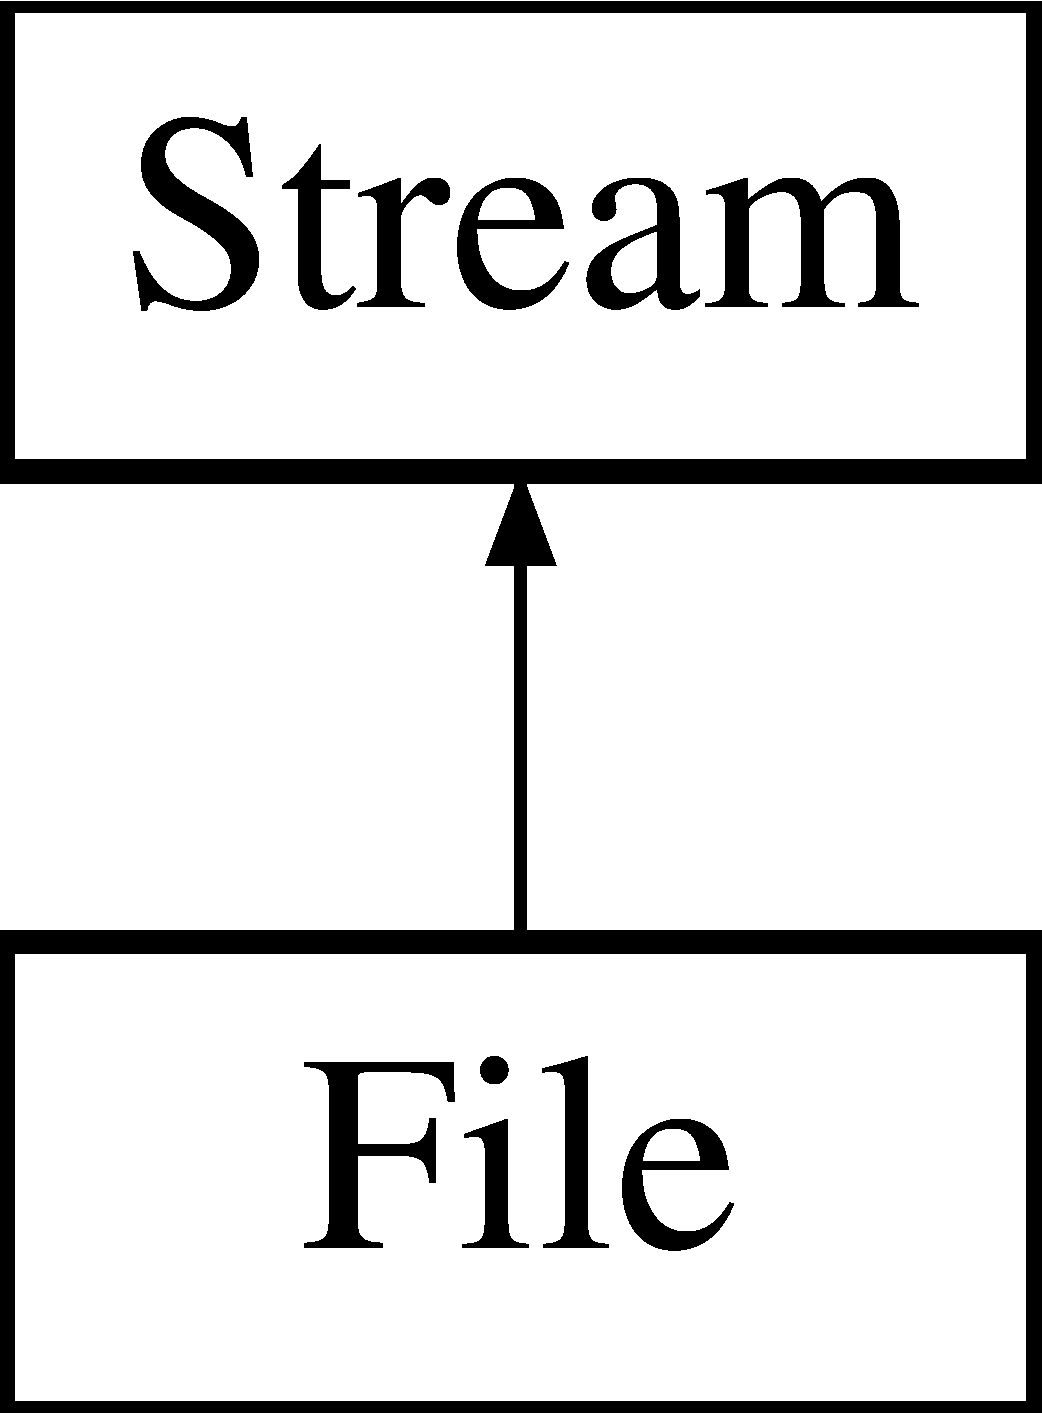
\includegraphics[height=2.000000cm]{class_file}
\end{center}
\end{figure}
\subsection*{Public Member Functions}
\begin{DoxyCompactItemize}
\item 
\hypertarget{class_file_ad34490d697d9e56859f566534b360c54}{}{\bfseries File} (\hyperlink{class_sd_file}{Sd\+File} f, const char $\ast$name)\label{class_file_ad34490d697d9e56859f566534b360c54}

\item 
\hypertarget{class_file_acee911dcb9057b964fd5b3ce888a934b}{}virtual size\+\_\+t {\bfseries write} (uint8\+\_\+t)\label{class_file_acee911dcb9057b964fd5b3ce888a934b}

\item 
\hypertarget{class_file_aa531c1641a2363e1f6b9d103f37433da}{}virtual size\+\_\+t {\bfseries write} (const uint8\+\_\+t $\ast$buf, size\+\_\+t size)\label{class_file_aa531c1641a2363e1f6b9d103f37433da}

\item 
\hypertarget{class_file_a4c46a1975e66c37977bf07c58ec10b4e}{}virtual int {\bfseries read} ()\label{class_file_a4c46a1975e66c37977bf07c58ec10b4e}

\item 
\hypertarget{class_file_a0e5025f39bd584563bfe4b05fc1db268}{}virtual int {\bfseries peek} ()\label{class_file_a0e5025f39bd584563bfe4b05fc1db268}

\item 
\hypertarget{class_file_acf613c4e75bae85f543b30e701ebcc44}{}virtual int {\bfseries available} ()\label{class_file_acf613c4e75bae85f543b30e701ebcc44}

\item 
\hypertarget{class_file_af87fa862de707575b8badd044a5af80e}{}virtual void {\bfseries flush} ()\label{class_file_af87fa862de707575b8badd044a5af80e}

\item 
\hypertarget{class_file_a30539792f063f24ee5ee7c11dfa564b2}{}int {\bfseries read} (void $\ast$buf, uint16\+\_\+t nbyte)\label{class_file_a30539792f063f24ee5ee7c11dfa564b2}

\item 
\hypertarget{class_file_a2a46cc148ddc53fe5170164227a695ae}{}boolean {\bfseries seek} (uint32\+\_\+t pos)\label{class_file_a2a46cc148ddc53fe5170164227a695ae}

\item 
\hypertarget{class_file_aae991c597c0bc4c5eb44c1f3b06a21ec}{}uint32\+\_\+t {\bfseries position} ()\label{class_file_aae991c597c0bc4c5eb44c1f3b06a21ec}

\item 
\hypertarget{class_file_a603d3cd3319142d00a7ebd434970b017}{}uint32\+\_\+t {\bfseries size} ()\label{class_file_a603d3cd3319142d00a7ebd434970b017}

\item 
\hypertarget{class_file_a83cbce54d6c3b8c2f417b51f6b3f488c}{}void {\bfseries close} ()\label{class_file_a83cbce54d6c3b8c2f417b51f6b3f488c}

\item 
\hypertarget{class_file_af171fbf441c899cf71d88b8b0b83d38b}{}{\bfseries operator bool} ()\label{class_file_af171fbf441c899cf71d88b8b0b83d38b}

\item 
\hypertarget{class_file_a7dc80cb96e6062652690a42b584f230e}{}char $\ast$ {\bfseries name} ()\label{class_file_a7dc80cb96e6062652690a42b584f230e}

\item 
\hypertarget{class_file_a532cb01e66c863f0a0c70bad3acbcdfe}{}boolean {\bfseries is\+Directory} (void)\label{class_file_a532cb01e66c863f0a0c70bad3acbcdfe}

\item 
\hypertarget{class_file_a19590302a57d1ba601a15fa44aeab643}{}\hyperlink{class_file}{File} {\bfseries open\+Next\+File} (uint8\+\_\+t mode=\hyperlink{_sd_fat_8h_ac13ca62d7e6f8f6d657d4607474652bf}{O\+\_\+\+R\+D\+O\+N\+L\+Y})\label{class_file_a19590302a57d1ba601a15fa44aeab643}

\item 
\hypertarget{class_file_a0fed2e25f4a38b19c57967d4bb6e3598}{}void {\bfseries rewind\+Directory} (void)\label{class_file_a0fed2e25f4a38b19c57967d4bb6e3598}

\end{DoxyCompactItemize}


The documentation for this class was generated from the following files\+:\begin{DoxyCompactItemize}
\item 
Sources/\+Engduino\+S\+D/src/S\+D.\+h\item 
Sources/\+Engduino\+S\+D/src/File.\+cpp\item 
Sources/\+Engduino\+S\+D/src/S\+D.\+cpp\end{DoxyCompactItemize}

\hypertarget{structmaster_boot_record}{}\section{master\+Boot\+Record Struct Reference}
\label{structmaster_boot_record}\index{master\+Boot\+Record@{master\+Boot\+Record}}


Master Boot Record.  




{\ttfamily \#include $<$Fat\+Structs.\+h$>$}

\subsection*{Public Attributes}
\begin{DoxyCompactItemize}
\item 
uint8\+\_\+t \hyperlink{structmaster_boot_record_a26ca1fb4ebbff2cc1a54153b1dfcd688}{code\+Area} \mbox{[}440\mbox{]}
\item 
uint32\+\_\+t \hyperlink{structmaster_boot_record_a77151c641444c0653ff71a253f0423ef}{disk\+Signature}
\item 
uint16\+\_\+t \hyperlink{structmaster_boot_record_afacfc863e98f64053cd9459c6dec948f}{usually\+Zero}
\item 
\hyperlink{_fat_structs_8h_a37251e7d5c69a159be727a3fc8c9d0e6}{part\+\_\+t} \hyperlink{structmaster_boot_record_aa4e294e50f311635c10c92f4c99227c5}{part} \mbox{[}4\mbox{]}
\item 
uint8\+\_\+t \hyperlink{structmaster_boot_record_a42b0b413ecb21ac5314d4f6bca05308f}{mbr\+Sig0}
\item 
uint8\+\_\+t \hyperlink{structmaster_boot_record_aafbbcb4f6a2d1181c6458d4c9603df4f}{mbr\+Sig1}
\end{DoxyCompactItemize}


\subsection{Detailed Description}
Master Boot Record. 

The first block of a storage device that is formatted with a M\+B\+R. 

\subsection{Member Data Documentation}
\hypertarget{structmaster_boot_record_a26ca1fb4ebbff2cc1a54153b1dfcd688}{}\index{master\+Boot\+Record@{master\+Boot\+Record}!code\+Area@{code\+Area}}
\index{code\+Area@{code\+Area}!master\+Boot\+Record@{master\+Boot\+Record}}
\subsubsection[{code\+Area}]{\setlength{\rightskip}{0pt plus 5cm}uint8\+\_\+t master\+Boot\+Record\+::code\+Area\mbox{[}440\mbox{]}}\label{structmaster_boot_record_a26ca1fb4ebbff2cc1a54153b1dfcd688}
Code Area for master boot program. \hypertarget{structmaster_boot_record_a77151c641444c0653ff71a253f0423ef}{}\index{master\+Boot\+Record@{master\+Boot\+Record}!disk\+Signature@{disk\+Signature}}
\index{disk\+Signature@{disk\+Signature}!master\+Boot\+Record@{master\+Boot\+Record}}
\subsubsection[{disk\+Signature}]{\setlength{\rightskip}{0pt plus 5cm}uint32\+\_\+t master\+Boot\+Record\+::disk\+Signature}\label{structmaster_boot_record_a77151c641444c0653ff71a253f0423ef}
Optional Windows\+N\+T disk signature. May contain more boot code. \hypertarget{structmaster_boot_record_a42b0b413ecb21ac5314d4f6bca05308f}{}\index{master\+Boot\+Record@{master\+Boot\+Record}!mbr\+Sig0@{mbr\+Sig0}}
\index{mbr\+Sig0@{mbr\+Sig0}!master\+Boot\+Record@{master\+Boot\+Record}}
\subsubsection[{mbr\+Sig0}]{\setlength{\rightskip}{0pt plus 5cm}uint8\+\_\+t master\+Boot\+Record\+::mbr\+Sig0}\label{structmaster_boot_record_a42b0b413ecb21ac5314d4f6bca05308f}
First M\+B\+R signature byte. Must be 0\+X55 \hypertarget{structmaster_boot_record_aafbbcb4f6a2d1181c6458d4c9603df4f}{}\index{master\+Boot\+Record@{master\+Boot\+Record}!mbr\+Sig1@{mbr\+Sig1}}
\index{mbr\+Sig1@{mbr\+Sig1}!master\+Boot\+Record@{master\+Boot\+Record}}
\subsubsection[{mbr\+Sig1}]{\setlength{\rightskip}{0pt plus 5cm}uint8\+\_\+t master\+Boot\+Record\+::mbr\+Sig1}\label{structmaster_boot_record_aafbbcb4f6a2d1181c6458d4c9603df4f}
Second M\+B\+R signature byte. Must be 0\+X\+A\+A \hypertarget{structmaster_boot_record_aa4e294e50f311635c10c92f4c99227c5}{}\index{master\+Boot\+Record@{master\+Boot\+Record}!part@{part}}
\index{part@{part}!master\+Boot\+Record@{master\+Boot\+Record}}
\subsubsection[{part}]{\setlength{\rightskip}{0pt plus 5cm}{\bf part\+\_\+t} master\+Boot\+Record\+::part\mbox{[}4\mbox{]}}\label{structmaster_boot_record_aa4e294e50f311635c10c92f4c99227c5}
Partition tables. \hypertarget{structmaster_boot_record_afacfc863e98f64053cd9459c6dec948f}{}\index{master\+Boot\+Record@{master\+Boot\+Record}!usually\+Zero@{usually\+Zero}}
\index{usually\+Zero@{usually\+Zero}!master\+Boot\+Record@{master\+Boot\+Record}}
\subsubsection[{usually\+Zero}]{\setlength{\rightskip}{0pt plus 5cm}uint16\+\_\+t master\+Boot\+Record\+::usually\+Zero}\label{structmaster_boot_record_afacfc863e98f64053cd9459c6dec948f}
Usually zero but may be more boot code. 

The documentation for this struct was generated from the following file\+:\begin{DoxyCompactItemize}
\item 
Sources/\+Engduino\+S\+D/src/utility/\hyperlink{_fat_structs_8h}{Fat\+Structs.\+h}\end{DoxyCompactItemize}

\hypertarget{structpartition_table}{}\section{partition\+Table Struct Reference}
\label{structpartition_table}\index{partition\+Table@{partition\+Table}}


M\+B\+R partition table entry.  




{\ttfamily \#include $<$Fat\+Structs.\+h$>$}

\subsection*{Public Attributes}
\begin{DoxyCompactItemize}
\item 
uint8\+\_\+t \hyperlink{structpartition_table_adf386afb1f33046d8b6a1a0afa780ec9}{boot}
\item 
uint8\+\_\+t \hyperlink{structpartition_table_a7d426694b8cf2151ae38568670a8c845}{begin\+Head}
\item 
unsigned \hyperlink{structpartition_table_ae201c11d9671c9efc307c654a2b6c026}{begin\+Sector}\+: 6
\item 
unsigned \hyperlink{structpartition_table_a744f0c7f9ad4c426b10de085b4f52392}{begin\+Cylinder\+High}\+: 2
\item 
uint8\+\_\+t \hyperlink{structpartition_table_a941fcb4df298f5f73ccca011bf40787a}{begin\+Cylinder\+Low}
\item 
uint8\+\_\+t \hyperlink{structpartition_table_a3861cf276c728c4dd30ca04e74197ee8}{type}
\item 
uint8\+\_\+t \hyperlink{structpartition_table_a4a3945bfd3a29f474984cb9f180dbd51}{end\+Head}
\item 
unsigned \hyperlink{structpartition_table_a27cdc4320c418ed0d833ab163ed77ad7}{end\+Sector}\+: 6
\item 
unsigned \hyperlink{structpartition_table_a32fea225b8ffd925ad919ffc56e9abda}{end\+Cylinder\+High}\+: 2
\item 
uint8\+\_\+t \hyperlink{structpartition_table_ad7829e34be70084abe145227b0d18274}{end\+Cylinder\+Low}
\item 
uint32\+\_\+t \hyperlink{structpartition_table_a02bbdff840c854dc96fa0b6da8589d86}{first\+Sector}
\item 
uint32\+\_\+t \hyperlink{structpartition_table_acf96e59ce648a9a0cf35751c3b6d7730}{total\+Sectors}
\end{DoxyCompactItemize}


\subsection{Detailed Description}
M\+B\+R partition table entry. 

A partition table entry for a M\+B\+R formatted storage device. The M\+B\+R partition table has four entries. 

\subsection{Member Data Documentation}
\hypertarget{structpartition_table_a744f0c7f9ad4c426b10de085b4f52392}{}\index{partition\+Table@{partition\+Table}!begin\+Cylinder\+High@{begin\+Cylinder\+High}}
\index{begin\+Cylinder\+High@{begin\+Cylinder\+High}!partition\+Table@{partition\+Table}}
\subsubsection[{begin\+Cylinder\+High}]{\setlength{\rightskip}{0pt plus 5cm}unsigned partition\+Table\+::begin\+Cylinder\+High}\label{structpartition_table_a744f0c7f9ad4c426b10de085b4f52392}
High bits cylinder for first block in partition. \hypertarget{structpartition_table_a941fcb4df298f5f73ccca011bf40787a}{}\index{partition\+Table@{partition\+Table}!begin\+Cylinder\+Low@{begin\+Cylinder\+Low}}
\index{begin\+Cylinder\+Low@{begin\+Cylinder\+Low}!partition\+Table@{partition\+Table}}
\subsubsection[{begin\+Cylinder\+Low}]{\setlength{\rightskip}{0pt plus 5cm}uint8\+\_\+t partition\+Table\+::begin\+Cylinder\+Low}\label{structpartition_table_a941fcb4df298f5f73ccca011bf40787a}
Combine begin\+Cylinder\+Low with begin\+Cylinder\+High. Legal values are 0-\/1023. Only used in old P\+C B\+I\+O\+S. \hypertarget{structpartition_table_a7d426694b8cf2151ae38568670a8c845}{}\index{partition\+Table@{partition\+Table}!begin\+Head@{begin\+Head}}
\index{begin\+Head@{begin\+Head}!partition\+Table@{partition\+Table}}
\subsubsection[{begin\+Head}]{\setlength{\rightskip}{0pt plus 5cm}uint8\+\_\+t partition\+Table\+::begin\+Head}\label{structpartition_table_a7d426694b8cf2151ae38568670a8c845}
Head part of Cylinder-\/head-\/sector address of the first block in the partition. Legal values are 0-\/255. Only used in old P\+C B\+I\+O\+S. \hypertarget{structpartition_table_ae201c11d9671c9efc307c654a2b6c026}{}\index{partition\+Table@{partition\+Table}!begin\+Sector@{begin\+Sector}}
\index{begin\+Sector@{begin\+Sector}!partition\+Table@{partition\+Table}}
\subsubsection[{begin\+Sector}]{\setlength{\rightskip}{0pt plus 5cm}unsigned partition\+Table\+::begin\+Sector}\label{structpartition_table_ae201c11d9671c9efc307c654a2b6c026}
Sector part of Cylinder-\/head-\/sector address of the first block in the partition. Legal values are 1-\/63. Only used in old P\+C B\+I\+O\+S. \hypertarget{structpartition_table_adf386afb1f33046d8b6a1a0afa780ec9}{}\index{partition\+Table@{partition\+Table}!boot@{boot}}
\index{boot@{boot}!partition\+Table@{partition\+Table}}
\subsubsection[{boot}]{\setlength{\rightskip}{0pt plus 5cm}uint8\+\_\+t partition\+Table\+::boot}\label{structpartition_table_adf386afb1f33046d8b6a1a0afa780ec9}
Boot Indicator . Indicates whether the volume is the active partition. Legal values include\+: 0\+X00. Do not use for booting. 0\+X80 Active partition. \hypertarget{structpartition_table_a32fea225b8ffd925ad919ffc56e9abda}{}\index{partition\+Table@{partition\+Table}!end\+Cylinder\+High@{end\+Cylinder\+High}}
\index{end\+Cylinder\+High@{end\+Cylinder\+High}!partition\+Table@{partition\+Table}}
\subsubsection[{end\+Cylinder\+High}]{\setlength{\rightskip}{0pt plus 5cm}unsigned partition\+Table\+::end\+Cylinder\+High}\label{structpartition_table_a32fea225b8ffd925ad919ffc56e9abda}
High bits of end cylinder \hypertarget{structpartition_table_ad7829e34be70084abe145227b0d18274}{}\index{partition\+Table@{partition\+Table}!end\+Cylinder\+Low@{end\+Cylinder\+Low}}
\index{end\+Cylinder\+Low@{end\+Cylinder\+Low}!partition\+Table@{partition\+Table}}
\subsubsection[{end\+Cylinder\+Low}]{\setlength{\rightskip}{0pt plus 5cm}uint8\+\_\+t partition\+Table\+::end\+Cylinder\+Low}\label{structpartition_table_ad7829e34be70084abe145227b0d18274}
Combine end\+Cylinder\+Low with end\+Cylinder\+High. Legal values are 0-\/1023. Only used in old P\+C B\+I\+O\+S. \hypertarget{structpartition_table_a4a3945bfd3a29f474984cb9f180dbd51}{}\index{partition\+Table@{partition\+Table}!end\+Head@{end\+Head}}
\index{end\+Head@{end\+Head}!partition\+Table@{partition\+Table}}
\subsubsection[{end\+Head}]{\setlength{\rightskip}{0pt plus 5cm}uint8\+\_\+t partition\+Table\+::end\+Head}\label{structpartition_table_a4a3945bfd3a29f474984cb9f180dbd51}
head part of cylinder-\/head-\/sector address of the last sector in the partition. Legal values are 0-\/255. Only used in old P\+C B\+I\+O\+S. \hypertarget{structpartition_table_a27cdc4320c418ed0d833ab163ed77ad7}{}\index{partition\+Table@{partition\+Table}!end\+Sector@{end\+Sector}}
\index{end\+Sector@{end\+Sector}!partition\+Table@{partition\+Table}}
\subsubsection[{end\+Sector}]{\setlength{\rightskip}{0pt plus 5cm}unsigned partition\+Table\+::end\+Sector}\label{structpartition_table_a27cdc4320c418ed0d833ab163ed77ad7}
Sector part of cylinder-\/head-\/sector address of the last sector in the partition. Legal values are 1-\/63. Only used in old P\+C B\+I\+O\+S. \hypertarget{structpartition_table_a02bbdff840c854dc96fa0b6da8589d86}{}\index{partition\+Table@{partition\+Table}!first\+Sector@{first\+Sector}}
\index{first\+Sector@{first\+Sector}!partition\+Table@{partition\+Table}}
\subsubsection[{first\+Sector}]{\setlength{\rightskip}{0pt plus 5cm}uint32\+\_\+t partition\+Table\+::first\+Sector}\label{structpartition_table_a02bbdff840c854dc96fa0b6da8589d86}
Logical block address of the first block in the partition. \hypertarget{structpartition_table_acf96e59ce648a9a0cf35751c3b6d7730}{}\index{partition\+Table@{partition\+Table}!total\+Sectors@{total\+Sectors}}
\index{total\+Sectors@{total\+Sectors}!partition\+Table@{partition\+Table}}
\subsubsection[{total\+Sectors}]{\setlength{\rightskip}{0pt plus 5cm}uint32\+\_\+t partition\+Table\+::total\+Sectors}\label{structpartition_table_acf96e59ce648a9a0cf35751c3b6d7730}
Length of the partition, in blocks. \hypertarget{structpartition_table_a3861cf276c728c4dd30ca04e74197ee8}{}\index{partition\+Table@{partition\+Table}!type@{type}}
\index{type@{type}!partition\+Table@{partition\+Table}}
\subsubsection[{type}]{\setlength{\rightskip}{0pt plus 5cm}uint8\+\_\+t partition\+Table\+::type}\label{structpartition_table_a3861cf276c728c4dd30ca04e74197ee8}
Partition type. See defines that begin with P\+A\+R\+T\+\_\+\+T\+Y\+P\+E\+\_\+ for some Microsoft partition types. 

The documentation for this struct was generated from the following file\+:\begin{DoxyCompactItemize}
\item 
Sources/\+Engduino\+S\+D/src/utility/\hyperlink{_fat_structs_8h}{Fat\+Structs.\+h}\end{DoxyCompactItemize}

\hypertarget{class_sd2_card}{}\section{Sd2\+Card Class Reference}
\label{class_sd2_card}\index{Sd2\+Card@{Sd2\+Card}}


Raw access to S\+D and S\+D\+H\+C flash memory cards.  




{\ttfamily \#include $<$Sd2\+Card.\+h$>$}

\subsection*{Public Member Functions}
\begin{DoxyCompactItemize}
\item 
\hyperlink{class_sd2_card_af85a5ec4f5f4ec89deb8936c3fd7de65}{Sd2\+Card} (void)
\item 
uint32\+\_\+t \hyperlink{class_sd2_card_a862473431cc314238bfccdc531a70d3a}{card\+Size} (void)
\item 
uint8\+\_\+t \hyperlink{class_sd2_card_af49fb720fad1d3ea9f5782da0d87fc0b}{erase} (uint32\+\_\+t first\+Block, uint32\+\_\+t last\+Block)
\item 
uint8\+\_\+t \hyperlink{class_sd2_card_a2e3998f6e910a2936d3ef54bf082b2ce}{erase\+Single\+Block\+Enable} (void)
\item 
uint8\+\_\+t \hyperlink{class_sd2_card_adfa5b1a39875236dff591acbd560bfe7}{error\+Code} (void) const 
\item 
uint8\+\_\+t \hyperlink{class_sd2_card_a13fed56bd5bcfee862acb6de6924936c}{error\+Data} (void) const 
\item 
uint8\+\_\+t \hyperlink{class_sd2_card_afaec9a22060626b02c07a09eff2e9113}{init} (void)
\item 
uint8\+\_\+t \hyperlink{class_sd2_card_ad99b2d2156c9746065c52839ef679354}{init} (uint8\+\_\+t sck\+Rate\+I\+D)
\item 
uint8\+\_\+t \hyperlink{class_sd2_card_a919c789eb9b140426c706f0862780978}{init} (uint8\+\_\+t sck\+Rate\+I\+D, uint8\+\_\+t chip\+Select\+Pin)
\item 
void \hyperlink{class_sd2_card_aa279ac05b3f25acbf10cc424a25750da}{partial\+Block\+Read} (uint8\+\_\+t value)
\item 
uint8\+\_\+t \hyperlink{class_sd2_card_a73ad7fee10e05439f6ec832ce0eb196f}{partial\+Block\+Read} (void) const 
\item 
uint8\+\_\+t \hyperlink{class_sd2_card_ae26d840449a42d45af464fb81b92e2ab}{read\+Block} (uint32\+\_\+t block, uint8\+\_\+t $\ast$dst)
\item 
uint8\+\_\+t \hyperlink{class_sd2_card_ae2d1396ad30081b4201cd372358ef699}{read\+Data} (uint32\+\_\+t block, uint16\+\_\+t offset, uint16\+\_\+t count, uint8\+\_\+t $\ast$dst)
\item 
uint8\+\_\+t \hyperlink{class_sd2_card_aee2be03d649548e2ab26033f18638d19}{read\+C\+I\+D} (\hyperlink{struct_c_i_d}{cid\+\_\+t} $\ast$cid)
\item 
uint8\+\_\+t \hyperlink{class_sd2_card_a79845d8d4593cb3b1b7641ba27edddfb}{read\+C\+S\+D} (\hyperlink{unioncsd__t}{csd\+\_\+t} $\ast$csd)
\item 
void \hyperlink{class_sd2_card_a0de961537d051bbcafd87ed9fff5fe48}{read\+End} (void)
\item 
uint8\+\_\+t \hyperlink{class_sd2_card_ad849b8896de9abd4e24bd98f4204ccc4}{set\+Sck\+Rate} (uint8\+\_\+t sck\+Rate\+I\+D)
\item 
uint8\+\_\+t \hyperlink{class_sd2_card_a3ba97504f5928c932c346101d3dabfd2}{type} (void) const 
\item 
uint8\+\_\+t \hyperlink{class_sd2_card_ae9bdd6cff43b8b694584f9bae7e781b0}{write\+Block} (uint32\+\_\+t block\+Number, const uint8\+\_\+t $\ast$src)
\item 
uint8\+\_\+t \hyperlink{class_sd2_card_af602d107e1ead2d0971e9f4c7b744cf8}{write\+Data} (const uint8\+\_\+t $\ast$src)
\item 
uint8\+\_\+t \hyperlink{class_sd2_card_a82a21a07fdfe45c5c75d486a13cded8a}{write\+Start} (uint32\+\_\+t block\+Number, uint32\+\_\+t erase\+Count)
\item 
uint8\+\_\+t \hyperlink{class_sd2_card_a3a60481c0821606546a85d056bb96f47}{write\+Stop} (void)
\end{DoxyCompactItemize}


\subsection{Detailed Description}
Raw access to S\+D and S\+D\+H\+C flash memory cards. 

\subsection{Constructor \& Destructor Documentation}
\hypertarget{class_sd2_card_af85a5ec4f5f4ec89deb8936c3fd7de65}{}\index{Sd2\+Card@{Sd2\+Card}!Sd2\+Card@{Sd2\+Card}}
\index{Sd2\+Card@{Sd2\+Card}!Sd2\+Card@{Sd2\+Card}}
\subsubsection[{Sd2\+Card}]{\setlength{\rightskip}{0pt plus 5cm}Sd2\+Card\+::\+Sd2\+Card (
\begin{DoxyParamCaption}
\item[{void}]{}
\end{DoxyParamCaption}
)\hspace{0.3cm}{\ttfamily [inline]}}\label{class_sd2_card_af85a5ec4f5f4ec89deb8936c3fd7de65}
Construct an instance of \hyperlink{class_sd2_card}{Sd2\+Card}. 

\subsection{Member Function Documentation}
\hypertarget{class_sd2_card_a862473431cc314238bfccdc531a70d3a}{}\index{Sd2\+Card@{Sd2\+Card}!card\+Size@{card\+Size}}
\index{card\+Size@{card\+Size}!Sd2\+Card@{Sd2\+Card}}
\subsubsection[{card\+Size}]{\setlength{\rightskip}{0pt plus 5cm}uint32\+\_\+t Sd2\+Card\+::card\+Size (
\begin{DoxyParamCaption}
\item[{void}]{}
\end{DoxyParamCaption}
)}\label{class_sd2_card_a862473431cc314238bfccdc531a70d3a}
Determine the size of an S\+D flash memory card.

\begin{DoxyReturn}{Returns}
The number of 512 byte data blocks in the card or zero if an error occurs. 
\end{DoxyReturn}
\hypertarget{class_sd2_card_af49fb720fad1d3ea9f5782da0d87fc0b}{}\index{Sd2\+Card@{Sd2\+Card}!erase@{erase}}
\index{erase@{erase}!Sd2\+Card@{Sd2\+Card}}
\subsubsection[{erase}]{\setlength{\rightskip}{0pt plus 5cm}uint8\+\_\+t Sd2\+Card\+::erase (
\begin{DoxyParamCaption}
\item[{uint32\+\_\+t}]{first\+Block, }
\item[{uint32\+\_\+t}]{last\+Block}
\end{DoxyParamCaption}
)}\label{class_sd2_card_af49fb720fad1d3ea9f5782da0d87fc0b}
Erase a range of blocks.


\begin{DoxyParams}[1]{Parameters}
\mbox{\tt in}  & {\em first\+Block} & The address of the first block in the range. \\
\hline
\mbox{\tt in}  & {\em last\+Block} & The address of the last block in the range.\\
\hline
\end{DoxyParams}
\begin{DoxyNote}{Note}
This function requests the S\+D card to do a flash erase for a range of blocks. The data on the card after an erase operation is either 0 or 1, depends on the card vendor. The card must support single block erase.
\end{DoxyNote}
\begin{DoxyReturn}{Returns}
The value one, true, is returned for success and the value zero, false, is returned for failure. 
\end{DoxyReturn}
\hypertarget{class_sd2_card_a2e3998f6e910a2936d3ef54bf082b2ce}{}\index{Sd2\+Card@{Sd2\+Card}!erase\+Single\+Block\+Enable@{erase\+Single\+Block\+Enable}}
\index{erase\+Single\+Block\+Enable@{erase\+Single\+Block\+Enable}!Sd2\+Card@{Sd2\+Card}}
\subsubsection[{erase\+Single\+Block\+Enable}]{\setlength{\rightskip}{0pt plus 5cm}uint8\+\_\+t Sd2\+Card\+::erase\+Single\+Block\+Enable (
\begin{DoxyParamCaption}
\item[{void}]{}
\end{DoxyParamCaption}
)}\label{class_sd2_card_a2e3998f6e910a2936d3ef54bf082b2ce}
Determine if card supports single block erase.

\begin{DoxyReturn}{Returns}
The value one, true, is returned if single block erase is supported. The value zero, false, is returned if single block erase is not supported. 
\end{DoxyReturn}
\hypertarget{class_sd2_card_adfa5b1a39875236dff591acbd560bfe7}{}\index{Sd2\+Card@{Sd2\+Card}!error\+Code@{error\+Code}}
\index{error\+Code@{error\+Code}!Sd2\+Card@{Sd2\+Card}}
\subsubsection[{error\+Code}]{\setlength{\rightskip}{0pt plus 5cm}uint8\+\_\+t Sd2\+Card\+::error\+Code (
\begin{DoxyParamCaption}
\item[{void}]{}
\end{DoxyParamCaption}
) const\hspace{0.3cm}{\ttfamily [inline]}}\label{class_sd2_card_adfa5b1a39875236dff591acbd560bfe7}
\begin{DoxyReturn}{Returns}
error code for last error. See \hyperlink{_sd2_card_8h}{Sd2\+Card.\+h} for a list of error codes. 
\end{DoxyReturn}
\hypertarget{class_sd2_card_a13fed56bd5bcfee862acb6de6924936c}{}\index{Sd2\+Card@{Sd2\+Card}!error\+Data@{error\+Data}}
\index{error\+Data@{error\+Data}!Sd2\+Card@{Sd2\+Card}}
\subsubsection[{error\+Data}]{\setlength{\rightskip}{0pt plus 5cm}uint8\+\_\+t Sd2\+Card\+::error\+Data (
\begin{DoxyParamCaption}
\item[{void}]{}
\end{DoxyParamCaption}
) const\hspace{0.3cm}{\ttfamily [inline]}}\label{class_sd2_card_a13fed56bd5bcfee862acb6de6924936c}
\begin{DoxyReturn}{Returns}
error data for last error. 
\end{DoxyReturn}
\hypertarget{class_sd2_card_afaec9a22060626b02c07a09eff2e9113}{}\index{Sd2\+Card@{Sd2\+Card}!init@{init}}
\index{init@{init}!Sd2\+Card@{Sd2\+Card}}
\subsubsection[{init}]{\setlength{\rightskip}{0pt plus 5cm}uint8\+\_\+t Sd2\+Card\+::init (
\begin{DoxyParamCaption}
\item[{void}]{}
\end{DoxyParamCaption}
)\hspace{0.3cm}{\ttfamily [inline]}}\label{class_sd2_card_afaec9a22060626b02c07a09eff2e9113}
Initialize an S\+D flash memory card with default clock rate and chip select pin. See sd2\+Card\+::init(uint8\+\_\+t sck\+Rate\+I\+D, uint8\+\_\+t chip\+Select\+Pin). \hypertarget{class_sd2_card_ad99b2d2156c9746065c52839ef679354}{}\index{Sd2\+Card@{Sd2\+Card}!init@{init}}
\index{init@{init}!Sd2\+Card@{Sd2\+Card}}
\subsubsection[{init}]{\setlength{\rightskip}{0pt plus 5cm}uint8\+\_\+t Sd2\+Card\+::init (
\begin{DoxyParamCaption}
\item[{uint8\+\_\+t}]{sck\+Rate\+I\+D}
\end{DoxyParamCaption}
)\hspace{0.3cm}{\ttfamily [inline]}}\label{class_sd2_card_ad99b2d2156c9746065c52839ef679354}
Initialize an S\+D flash memory card with the selected S\+P\+I clock rate and the default S\+D chip select pin. See sd2\+Card\+::init(uint8\+\_\+t sck\+Rate\+I\+D, uint8\+\_\+t chip\+Select\+Pin). \hypertarget{class_sd2_card_a919c789eb9b140426c706f0862780978}{}\index{Sd2\+Card@{Sd2\+Card}!init@{init}}
\index{init@{init}!Sd2\+Card@{Sd2\+Card}}
\subsubsection[{init}]{\setlength{\rightskip}{0pt plus 5cm}uint8\+\_\+t Sd2\+Card\+::init (
\begin{DoxyParamCaption}
\item[{uint8\+\_\+t}]{sck\+Rate\+I\+D, }
\item[{uint8\+\_\+t}]{chip\+Select\+Pin}
\end{DoxyParamCaption}
)}\label{class_sd2_card_a919c789eb9b140426c706f0862780978}
Initialize an S\+D flash memory card.


\begin{DoxyParams}[1]{Parameters}
\mbox{\tt in}  & {\em sck\+Rate\+I\+D} & S\+P\+I clock rate selector. See \hyperlink{class_sd2_card_ad849b8896de9abd4e24bd98f4204ccc4}{set\+Sck\+Rate()}. \\
\hline
\mbox{\tt in}  & {\em chip\+Select\+Pin} & S\+D chip select pin number.\\
\hline
\end{DoxyParams}
\begin{DoxyReturn}{Returns}
The value one, true, is returned for success and the value zero, false, is returned for failure. The reason for failure can be determined by calling \hyperlink{class_sd2_card_adfa5b1a39875236dff591acbd560bfe7}{error\+Code()} and \hyperlink{class_sd2_card_a13fed56bd5bcfee862acb6de6924936c}{error\+Data()}. 
\end{DoxyReturn}
\hypertarget{class_sd2_card_aa279ac05b3f25acbf10cc424a25750da}{}\index{Sd2\+Card@{Sd2\+Card}!partial\+Block\+Read@{partial\+Block\+Read}}
\index{partial\+Block\+Read@{partial\+Block\+Read}!Sd2\+Card@{Sd2\+Card}}
\subsubsection[{partial\+Block\+Read}]{\setlength{\rightskip}{0pt plus 5cm}void Sd2\+Card\+::partial\+Block\+Read (
\begin{DoxyParamCaption}
\item[{uint8\+\_\+t}]{value}
\end{DoxyParamCaption}
)}\label{class_sd2_card_aa279ac05b3f25acbf10cc424a25750da}
Enable or disable partial block reads.

Enabling partial block reads improves performance by allowing a block to be read over the S\+P\+I bus as several sub-\/blocks. Errors may occur if the time between reads is too long since the S\+D card may timeout. The S\+P\+I S\+S line will be held low until the entire block is read or \hyperlink{class_sd2_card_a0de961537d051bbcafd87ed9fff5fe48}{read\+End()} is called.

Use this for applications like the Adafruit Wave Shield.


\begin{DoxyParams}[1]{Parameters}
\mbox{\tt in}  & {\em value} & The value T\+R\+U\+E (non-\/zero) or F\+A\+L\+S\+E (zero).) \\
\hline
\end{DoxyParams}
\hypertarget{class_sd2_card_a73ad7fee10e05439f6ec832ce0eb196f}{}\index{Sd2\+Card@{Sd2\+Card}!partial\+Block\+Read@{partial\+Block\+Read}}
\index{partial\+Block\+Read@{partial\+Block\+Read}!Sd2\+Card@{Sd2\+Card}}
\subsubsection[{partial\+Block\+Read}]{\setlength{\rightskip}{0pt plus 5cm}uint8\+\_\+t Sd2\+Card\+::partial\+Block\+Read (
\begin{DoxyParamCaption}
\item[{void}]{}
\end{DoxyParamCaption}
) const\hspace{0.3cm}{\ttfamily [inline]}}\label{class_sd2_card_a73ad7fee10e05439f6ec832ce0eb196f}
Returns the current value, true or false, for partial block read. \hypertarget{class_sd2_card_ae26d840449a42d45af464fb81b92e2ab}{}\index{Sd2\+Card@{Sd2\+Card}!read\+Block@{read\+Block}}
\index{read\+Block@{read\+Block}!Sd2\+Card@{Sd2\+Card}}
\subsubsection[{read\+Block}]{\setlength{\rightskip}{0pt plus 5cm}uint8\+\_\+t Sd2\+Card\+::read\+Block (
\begin{DoxyParamCaption}
\item[{uint32\+\_\+t}]{block, }
\item[{uint8\+\_\+t $\ast$}]{dst}
\end{DoxyParamCaption}
)}\label{class_sd2_card_ae26d840449a42d45af464fb81b92e2ab}
Read a 512 byte block from an S\+D card device.


\begin{DoxyParams}[1]{Parameters}
\mbox{\tt in}  & {\em block} & Logical block to be read. \\
\hline
\mbox{\tt out}  & {\em dst} & Pointer to the location that will receive the data.\\
\hline
\end{DoxyParams}
\begin{DoxyReturn}{Returns}
The value one, true, is returned for success and the value zero, false, is returned for failure. 
\end{DoxyReturn}
\hypertarget{class_sd2_card_aee2be03d649548e2ab26033f18638d19}{}\index{Sd2\+Card@{Sd2\+Card}!read\+C\+I\+D@{read\+C\+I\+D}}
\index{read\+C\+I\+D@{read\+C\+I\+D}!Sd2\+Card@{Sd2\+Card}}
\subsubsection[{read\+C\+I\+D}]{\setlength{\rightskip}{0pt plus 5cm}uint8\+\_\+t Sd2\+Card\+::read\+C\+I\+D (
\begin{DoxyParamCaption}
\item[{{\bf cid\+\_\+t} $\ast$}]{cid}
\end{DoxyParamCaption}
)\hspace{0.3cm}{\ttfamily [inline]}}\label{class_sd2_card_aee2be03d649548e2ab26033f18638d19}
Read a cards \hyperlink{struct_c_i_d}{C\+I\+D} register. The \hyperlink{struct_c_i_d}{C\+I\+D} contains card identification information such as Manufacturer I\+D, Product name, Product serial number and Manufacturing date. \hypertarget{class_sd2_card_a79845d8d4593cb3b1b7641ba27edddfb}{}\index{Sd2\+Card@{Sd2\+Card}!read\+C\+S\+D@{read\+C\+S\+D}}
\index{read\+C\+S\+D@{read\+C\+S\+D}!Sd2\+Card@{Sd2\+Card}}
\subsubsection[{read\+C\+S\+D}]{\setlength{\rightskip}{0pt plus 5cm}uint8\+\_\+t Sd2\+Card\+::read\+C\+S\+D (
\begin{DoxyParamCaption}
\item[{{\bf csd\+\_\+t} $\ast$}]{csd}
\end{DoxyParamCaption}
)\hspace{0.3cm}{\ttfamily [inline]}}\label{class_sd2_card_a79845d8d4593cb3b1b7641ba27edddfb}
Read a cards C\+S\+D register. The C\+S\+D contains Card-\/\+Specific Data that provides information regarding access to the card\textquotesingle{}s contents. \hypertarget{class_sd2_card_ae2d1396ad30081b4201cd372358ef699}{}\index{Sd2\+Card@{Sd2\+Card}!read\+Data@{read\+Data}}
\index{read\+Data@{read\+Data}!Sd2\+Card@{Sd2\+Card}}
\subsubsection[{read\+Data}]{\setlength{\rightskip}{0pt plus 5cm}uint8\+\_\+t Sd2\+Card\+::read\+Data (
\begin{DoxyParamCaption}
\item[{uint32\+\_\+t}]{block, }
\item[{uint16\+\_\+t}]{offset, }
\item[{uint16\+\_\+t}]{count, }
\item[{uint8\+\_\+t $\ast$}]{dst}
\end{DoxyParamCaption}
)}\label{class_sd2_card_ae2d1396ad30081b4201cd372358ef699}
Read part of a 512 byte block from an S\+D card.


\begin{DoxyParams}[1]{Parameters}
\mbox{\tt in}  & {\em block} & Logical block to be read. \\
\hline
\mbox{\tt in}  & {\em offset} & Number of bytes to skip at start of block \\
\hline
\mbox{\tt out}  & {\em dst} & Pointer to the location that will receive the data. \\
\hline
\mbox{\tt in}  & {\em count} & Number of bytes to read \\
\hline
\end{DoxyParams}
\begin{DoxyReturn}{Returns}
The value one, true, is returned for success and the value zero, false, is returned for failure. 
\end{DoxyReturn}
\hypertarget{class_sd2_card_a0de961537d051bbcafd87ed9fff5fe48}{}\index{Sd2\+Card@{Sd2\+Card}!read\+End@{read\+End}}
\index{read\+End@{read\+End}!Sd2\+Card@{Sd2\+Card}}
\subsubsection[{read\+End}]{\setlength{\rightskip}{0pt plus 5cm}void Sd2\+Card\+::read\+End (
\begin{DoxyParamCaption}
\item[{void}]{}
\end{DoxyParamCaption}
)}\label{class_sd2_card_a0de961537d051bbcafd87ed9fff5fe48}
Skip remaining data in a block when in partial block read mode. \hypertarget{class_sd2_card_ad849b8896de9abd4e24bd98f4204ccc4}{}\index{Sd2\+Card@{Sd2\+Card}!set\+Sck\+Rate@{set\+Sck\+Rate}}
\index{set\+Sck\+Rate@{set\+Sck\+Rate}!Sd2\+Card@{Sd2\+Card}}
\subsubsection[{set\+Sck\+Rate}]{\setlength{\rightskip}{0pt plus 5cm}uint8\+\_\+t Sd2\+Card\+::set\+Sck\+Rate (
\begin{DoxyParamCaption}
\item[{uint8\+\_\+t}]{sck\+Rate\+I\+D}
\end{DoxyParamCaption}
)}\label{class_sd2_card_ad849b8896de9abd4e24bd98f4204ccc4}
Set the S\+P\+I clock rate.


\begin{DoxyParams}[1]{Parameters}
\mbox{\tt in}  & {\em sck\+Rate\+I\+D} & A value in the range \mbox{[}0, 6\mbox{]}.\\
\hline
\end{DoxyParams}
The S\+P\+I clock will be set to F\+\_\+\+C\+P\+U/pow(2, 1 + sck\+Rate\+I\+D). The maximum S\+P\+I rate is F\+\_\+\+C\+P\+U/2 for {\itshape sck\+Rate\+I\+D} = 0 and the minimum rate is F\+\_\+\+C\+P\+U/128 for {\itshape scs\+Rate\+I\+D} = 6.

\begin{DoxyReturn}{Returns}
The value one, true, is returned for success and the value zero, false, is returned for an invalid value of {\itshape sck\+Rate\+I\+D}. 
\end{DoxyReturn}
\hypertarget{class_sd2_card_a3ba97504f5928c932c346101d3dabfd2}{}\index{Sd2\+Card@{Sd2\+Card}!type@{type}}
\index{type@{type}!Sd2\+Card@{Sd2\+Card}}
\subsubsection[{type}]{\setlength{\rightskip}{0pt plus 5cm}uint8\+\_\+t Sd2\+Card\+::type (
\begin{DoxyParamCaption}
\item[{void}]{}
\end{DoxyParamCaption}
) const\hspace{0.3cm}{\ttfamily [inline]}}\label{class_sd2_card_a3ba97504f5928c932c346101d3dabfd2}
Return the card type\+: S\+D V1, S\+D V2 or S\+D\+H\+C \hypertarget{class_sd2_card_ae9bdd6cff43b8b694584f9bae7e781b0}{}\index{Sd2\+Card@{Sd2\+Card}!write\+Block@{write\+Block}}
\index{write\+Block@{write\+Block}!Sd2\+Card@{Sd2\+Card}}
\subsubsection[{write\+Block}]{\setlength{\rightskip}{0pt plus 5cm}uint8\+\_\+t Sd2\+Card\+::write\+Block (
\begin{DoxyParamCaption}
\item[{uint32\+\_\+t}]{block\+Number, }
\item[{const uint8\+\_\+t $\ast$}]{src}
\end{DoxyParamCaption}
)}\label{class_sd2_card_ae9bdd6cff43b8b694584f9bae7e781b0}
Writes a 512 byte block to an S\+D card.


\begin{DoxyParams}[1]{Parameters}
\mbox{\tt in}  & {\em block\+Number} & Logical block to be written. \\
\hline
\mbox{\tt in}  & {\em src} & Pointer to the location of the data to be written. \\
\hline
\end{DoxyParams}
\begin{DoxyReturn}{Returns}
The value one, true, is returned for success and the value zero, false, is returned for failure. 
\end{DoxyReturn}
\hypertarget{class_sd2_card_af602d107e1ead2d0971e9f4c7b744cf8}{}\index{Sd2\+Card@{Sd2\+Card}!write\+Data@{write\+Data}}
\index{write\+Data@{write\+Data}!Sd2\+Card@{Sd2\+Card}}
\subsubsection[{write\+Data}]{\setlength{\rightskip}{0pt plus 5cm}uint8\+\_\+t Sd2\+Card\+::write\+Data (
\begin{DoxyParamCaption}
\item[{const uint8\+\_\+t $\ast$}]{src}
\end{DoxyParamCaption}
)}\label{class_sd2_card_af602d107e1ead2d0971e9f4c7b744cf8}
Write one data block in a multiple block write sequence \hypertarget{class_sd2_card_a82a21a07fdfe45c5c75d486a13cded8a}{}\index{Sd2\+Card@{Sd2\+Card}!write\+Start@{write\+Start}}
\index{write\+Start@{write\+Start}!Sd2\+Card@{Sd2\+Card}}
\subsubsection[{write\+Start}]{\setlength{\rightskip}{0pt plus 5cm}uint8\+\_\+t Sd2\+Card\+::write\+Start (
\begin{DoxyParamCaption}
\item[{uint32\+\_\+t}]{block\+Number, }
\item[{uint32\+\_\+t}]{erase\+Count}
\end{DoxyParamCaption}
)}\label{class_sd2_card_a82a21a07fdfe45c5c75d486a13cded8a}
Start a write multiple blocks sequence.


\begin{DoxyParams}[1]{Parameters}
\mbox{\tt in}  & {\em block\+Number} & Address of first block in sequence. \\
\hline
\mbox{\tt in}  & {\em erase\+Count} & The number of blocks to be pre-\/erased.\\
\hline
\end{DoxyParams}
\begin{DoxyNote}{Note}
This function is used with \hyperlink{class_sd2_card_af602d107e1ead2d0971e9f4c7b744cf8}{write\+Data()} and \hyperlink{class_sd2_card_a3a60481c0821606546a85d056bb96f47}{write\+Stop()} for optimized multiple block writes.
\end{DoxyNote}
\begin{DoxyReturn}{Returns}
The value one, true, is returned for success and the value zero, false, is returned for failure. 
\end{DoxyReturn}
\hypertarget{class_sd2_card_a3a60481c0821606546a85d056bb96f47}{}\index{Sd2\+Card@{Sd2\+Card}!write\+Stop@{write\+Stop}}
\index{write\+Stop@{write\+Stop}!Sd2\+Card@{Sd2\+Card}}
\subsubsection[{write\+Stop}]{\setlength{\rightskip}{0pt plus 5cm}uint8\+\_\+t Sd2\+Card\+::write\+Stop (
\begin{DoxyParamCaption}
\item[{void}]{}
\end{DoxyParamCaption}
)}\label{class_sd2_card_a3a60481c0821606546a85d056bb96f47}
End a write multiple blocks sequence.

\begin{DoxyReturn}{Returns}
The value one, true, is returned for success and the value zero, false, is returned for failure. 
\end{DoxyReturn}


The documentation for this class was generated from the following files\+:\begin{DoxyCompactItemize}
\item 
Sources/\+Engduino\+S\+D/src/utility/\hyperlink{_sd2_card_8h}{Sd2\+Card.\+h}\item 
Sources/\+Engduino\+S\+D/src/utility/Sd2\+Card.\+cpp\end{DoxyCompactItemize}

\hypertarget{class_s_d_class}{}\section{S\+D\+Class Class Reference}
\label{class_s_d_class}\index{S\+D\+Class@{S\+D\+Class}}
\subsection*{Public Member Functions}
\begin{DoxyCompactItemize}
\item 
\hypertarget{class_s_d_class_aec226b7ad1f7db8b21b9d625cde89356}{}boolean {\bfseries begin} (uint8\+\_\+t cs\+Pin=\hyperlink{_sd2_card_8h_ae6b17538c14ba6c91ccb513db2c4c29c}{S\+D\+\_\+\+C\+H\+I\+P\+\_\+\+S\+E\+L\+E\+C\+T\+\_\+\+P\+I\+N})\label{class_s_d_class_aec226b7ad1f7db8b21b9d625cde89356}

\item 
\hypertarget{class_s_d_class_a02207388d102649d4a17901183c13f18}{}\hyperlink{class_file}{File} {\bfseries open} (const char $\ast$filename, uint8\+\_\+t mode=F\+I\+L\+E\+\_\+\+R\+E\+A\+D)\label{class_s_d_class_a02207388d102649d4a17901183c13f18}

\item 
\hypertarget{class_s_d_class_a0d9347b5446756f7f4dee9dd0c93fe5d}{}boolean {\bfseries exists} (char $\ast$filepath)\label{class_s_d_class_a0d9347b5446756f7f4dee9dd0c93fe5d}

\item 
\hypertarget{class_s_d_class_adb5edef260fcd12f2cc1e516d4d3b4a6}{}boolean {\bfseries mkdir} (char $\ast$filepath)\label{class_s_d_class_adb5edef260fcd12f2cc1e516d4d3b4a6}

\item 
\hypertarget{class_s_d_class_a0286f8bb49b66dfc1f7b176af9e6694b}{}boolean {\bfseries remove} (char $\ast$filepath)\label{class_s_d_class_a0286f8bb49b66dfc1f7b176af9e6694b}

\item 
\hypertarget{class_s_d_class_a484b22ac8e9506474a4fc738e6f3d71e}{}boolean {\bfseries rmdir} (char $\ast$filepath)\label{class_s_d_class_a484b22ac8e9506474a4fc738e6f3d71e}

\end{DoxyCompactItemize}
\subsection*{Friends}
\begin{DoxyCompactItemize}
\item 
\hypertarget{class_s_d_class_a68d15876ad188b7628261b12d0eac8aa}{}class {\bfseries File}\label{class_s_d_class_a68d15876ad188b7628261b12d0eac8aa}

\item 
\hypertarget{class_s_d_class_a8446a505a6d0edaccab9e8ff4002eae4}{}boolean {\bfseries callback\+\_\+open\+Path} (\hyperlink{class_sd_file}{Sd\+File} \&, char $\ast$, boolean, void $\ast$)\label{class_s_d_class_a8446a505a6d0edaccab9e8ff4002eae4}

\end{DoxyCompactItemize}


The documentation for this class was generated from the following files\+:\begin{DoxyCompactItemize}
\item 
Sources/\+Engduino\+S\+D/src/S\+D.\+h\item 
Sources/\+Engduino\+S\+D/src/S\+D.\+cpp\end{DoxyCompactItemize}

\hypertarget{class_sd_file}{}\section{Sd\+File Class Reference}
\label{class_sd_file}\index{Sd\+File@{Sd\+File}}


Access F\+A\+T16 and F\+A\+T32 files on S\+D and S\+D\+H\+C cards.  




{\ttfamily \#include $<$Sd\+Fat.\+h$>$}

Inheritance diagram for Sd\+File\+:\begin{figure}[H]
\begin{center}
\leavevmode
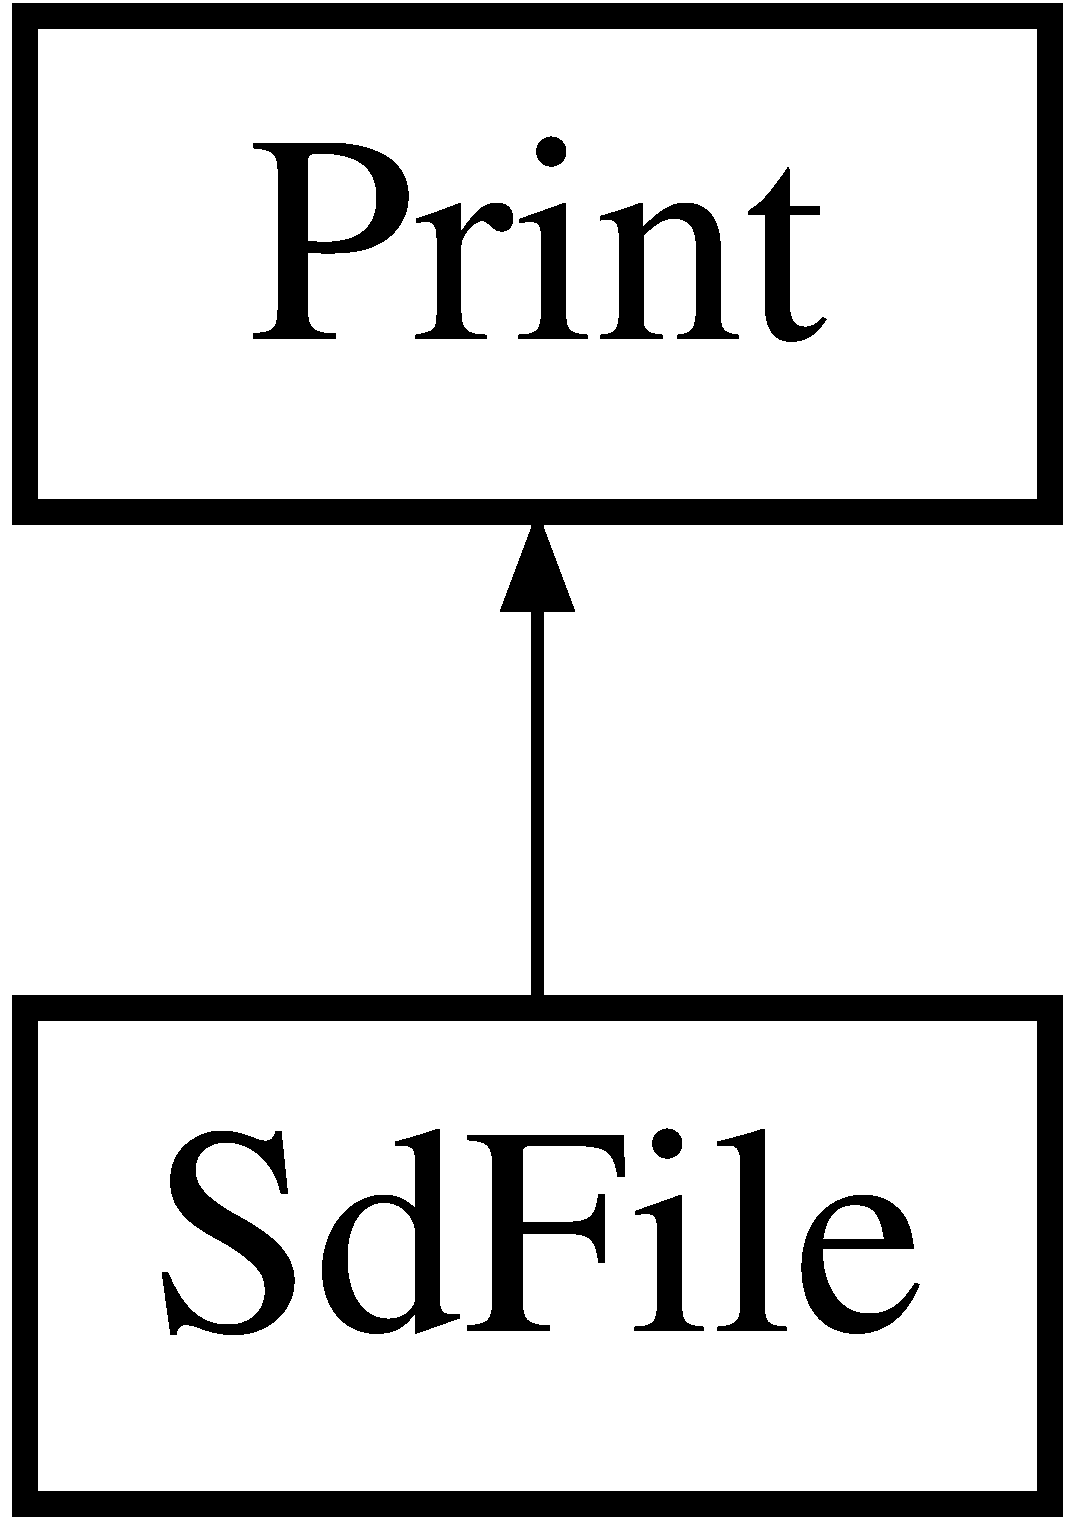
\includegraphics[height=2.000000cm]{class_sd_file}
\end{center}
\end{figure}
\subsection*{Public Member Functions}
\begin{DoxyCompactItemize}
\item 
\hyperlink{class_sd_file_a9e08675e64a4ef847700876d4291bbef}{Sd\+File} (void)
\item 
void \hyperlink{class_sd_file_a44c3d6ef602e84b8160a4d215faef7d4}{clear\+Unbuffered\+Read} (void)
\item 
uint8\+\_\+t \hyperlink{class_sd_file_a6b24350c89cc41ff644a343231a3983c}{close} (void)
\item 
uint8\+\_\+t \hyperlink{class_sd_file_a3b07fc09dbcb28ae7c89c060af6a1810}{contiguous\+Range} (uint32\+\_\+t $\ast$bgn\+Block, uint32\+\_\+t $\ast$end\+Block)
\item 
uint8\+\_\+t \hyperlink{class_sd_file_a07fc5c82318f073848e706f95830e5b5}{create\+Contiguous} (\hyperlink{class_sd_file}{Sd\+File} $\ast$dir\+File, const char $\ast$file\+Name, uint32\+\_\+t size)
\item 
uint32\+\_\+t \hyperlink{class_sd_file_ac5edd7e139aac981765b873da7b14c3d}{cur\+Cluster} (void) const 
\item 
uint32\+\_\+t \hyperlink{class_sd_file_a0fa8cd085c7059ced8d5f7855756ede2}{cur\+Position} (void) const 
\item 
uint32\+\_\+t \hyperlink{class_sd_file_a9cb63c516e40ff8aaca0ae23978bb95e}{dir\+Block} (void) const 
\item 
uint8\+\_\+t \hyperlink{class_sd_file_abaf9b1dc12d53cdeb937065edf68927d}{dir\+Entry} (\hyperlink{_fat_structs_8h_a803db59d4e16a0c54a647afc6a7954e3}{dir\+\_\+t} $\ast$dir)
\item 
uint8\+\_\+t \hyperlink{class_sd_file_a050c244681bb8d851e1e17bc3b387dca}{dir\+Index} (void) const 
\item 
uint32\+\_\+t \hyperlink{class_sd_file_ae9409305f9c2adb3650ab7b24093bfa1}{file\+Size} (void) const 
\item 
uint32\+\_\+t \hyperlink{class_sd_file_a593b7df10cf7a8d6a1fa2b6c12e130ac}{first\+Cluster} (void) const 
\item 
uint8\+\_\+t \hyperlink{class_sd_file_a8c656da3a6984395a70bee7932a2a933}{is\+Dir} (void) const 
\item 
uint8\+\_\+t \hyperlink{class_sd_file_a413b50bca08dd037756ae064e30f784c}{is\+File} (void) const 
\item 
uint8\+\_\+t \hyperlink{class_sd_file_a385a138ffead941e46a95b07d6327475}{is\+Open} (void) const 
\item 
uint8\+\_\+t \hyperlink{class_sd_file_a882e847b95aa47158d3df7ed7072d11e}{is\+Sub\+Dir} (void) const 
\item 
uint8\+\_\+t \hyperlink{class_sd_file_a0d0a535b287768e2ffa3b40c2e528ca4}{is\+Root} (void) const 
\item 
void \hyperlink{class_sd_file_afd9965ed8dee8bdd4d86dd14032edbc0}{ls} (uint8\+\_\+t flags=0, uint8\+\_\+t indent=0)
\item 
uint8\+\_\+t \hyperlink{class_sd_file_a62984bedf614a8de96b48bf9c5e7159f}{make\+Dir} (\hyperlink{class_sd_file}{Sd\+File} $\ast$dir, const char $\ast$\hyperlink{class_sd_file_ad7bbb106aa4c96c795c88b33def677bc}{dir\+Name})
\item 
uint8\+\_\+t \hyperlink{class_sd_file_a9e211ac14784f48aebb213194336f8cc}{open} (\hyperlink{class_sd_file}{Sd\+File} $\ast$dir\+File, uint16\+\_\+t index, uint8\+\_\+t oflag)
\item 
uint8\+\_\+t \hyperlink{class_sd_file_a3cf2167ad5ba6d84942ede8d2d07dcc6}{open} (\hyperlink{class_sd_file}{Sd\+File} $\ast$dir\+File, const char $\ast$file\+Name, uint8\+\_\+t oflag)
\item 
uint8\+\_\+t \hyperlink{class_sd_file_ac3612bc27eaf52a23d8cb85c8d96ad38}{open\+Root} (\hyperlink{class_sd_volume}{Sd\+Volume} $\ast$vol)
\item 
int16\+\_\+t \hyperlink{class_sd_file_a6c389f0180b4a86fb6d7464f50d3b0dd}{read} (void)
\item 
int16\+\_\+t \hyperlink{class_sd_file_a77ad85c5c80b34f8ebc57b5b89730554}{read} (void $\ast$buf, uint16\+\_\+t nbyte)
\item 
int8\+\_\+t \hyperlink{class_sd_file_ab240540b099cedcfe8b93b5e853d0628}{read\+Dir} (\hyperlink{_fat_structs_8h_a803db59d4e16a0c54a647afc6a7954e3}{dir\+\_\+t} $\ast$dir)
\item 
uint8\+\_\+t \hyperlink{class_sd_file_a66c5fb5f651a1ac319bab68fda1d3cc2}{remove} (void)
\item 
void \hyperlink{class_sd_file_afa8aaa7bdeb97b4e691ea01adf99f654}{rewind} (void)
\item 
uint8\+\_\+t \hyperlink{class_sd_file_a0d9e0c280b3469bb15e7258f6339746b}{rm\+Dir} (void)
\item 
uint8\+\_\+t \hyperlink{class_sd_file_a44c26fddfe2b42e7db3bc80290c77503}{rm\+Rf\+Star} (void)
\item 
uint8\+\_\+t \hyperlink{class_sd_file_aa95121ff038538e671f125160b280e9a}{seek\+Cur} (uint32\+\_\+t pos)
\item 
uint8\+\_\+t \hyperlink{class_sd_file_afa70bc7ba5eb789aee1b62fc5fafaa5b}{seek\+End} (void)
\item 
uint8\+\_\+t \hyperlink{class_sd_file_a5b8ea0ba6a9fec1ee8f1b11e90edb0c6}{seek\+Set} (uint32\+\_\+t pos)
\item 
void \hyperlink{class_sd_file_a08c9e76a4a7bb43fccf1dd5c72c66a16}{set\+Unbuffered\+Read} (void)
\item 
uint8\+\_\+t \hyperlink{class_sd_file_a249632ba9580c556c0b041d6b2aaf224}{timestamp} (uint8\+\_\+t flag, uint16\+\_\+t year, uint8\+\_\+t month, uint8\+\_\+t day, uint8\+\_\+t hour, uint8\+\_\+t minute, uint8\+\_\+t second)
\item 
uint8\+\_\+t \hyperlink{class_sd_file_a742d64ca964583ac3a92b31f0eba5e14}{sync} (void)
\item 
uint8\+\_\+t \hyperlink{class_sd_file_a3684bcce87f22a84f96cd342aa5a034b}{type} (void) const 
\item 
uint8\+\_\+t \hyperlink{class_sd_file_ade1e2b72f89b24f500502518fd678abd}{truncate} (uint32\+\_\+t size)
\item 
uint8\+\_\+t \hyperlink{class_sd_file_a6ce5bb460683272d8c86d02286622bb6}{unbuffered\+Read} (void) const 
\item 
\hyperlink{class_sd_volume}{Sd\+Volume} $\ast$ \hyperlink{class_sd_file_a96fbab54b98a17f2e4fd54c086fe1ff3}{volume} (void) const 
\item 
size\+\_\+t \hyperlink{class_sd_file_a67267a4b63d03a16e099195935613006}{write} (uint8\+\_\+t b)
\item 
size\+\_\+t \hyperlink{class_sd_file_a94d4541fda63b5390c8e97ebe815115a}{write} (const void $\ast$buf, uint16\+\_\+t nbyte)
\item 
size\+\_\+t \hyperlink{class_sd_file_ad74aaa9115724d663ee39e6dd2d808f8}{write} (const char $\ast$str)
\item 
uint8\+\_\+t \hyperlink{class_sd_file_a872927812be6c48a894bdfc72f1701a1}{contiguous\+Range} (uint32\+\_\+t \&bgn\+Block, uint32\+\_\+t \&end\+Block)
\item 
uint8\+\_\+t \hyperlink{class_sd_file_a231dd495e5c5997aea2a842481a68f40}{create\+Contiguous} (\hyperlink{class_sd_file}{Sd\+File} \&dir\+File, const char $\ast$file\+Name, uint32\+\_\+t size)
\item 
uint8\+\_\+t \hyperlink{class_sd_file_ae7b4b1057a1ee17f673c116771636156}{dir\+Entry} (\hyperlink{_fat_structs_8h_a803db59d4e16a0c54a647afc6a7954e3}{dir\+\_\+t} \&dir)
\item 
uint8\+\_\+t \hyperlink{class_sd_file_af87e166d0059d392d7038f68fca68529}{make\+Dir} (\hyperlink{class_sd_file}{Sd\+File} \&dir, const char $\ast$\hyperlink{class_sd_file_ad7bbb106aa4c96c795c88b33def677bc}{dir\+Name})
\item 
uint8\+\_\+t \hyperlink{class_sd_file_afe1d8ce70ef58ee5967005047064167c}{open} (\hyperlink{class_sd_file}{Sd\+File} \&dir\+File, const char $\ast$file\+Name, uint8\+\_\+t oflag)
\item 
uint8\+\_\+t \hyperlink{class_sd_file_a71e1c08dc4fb58b95554925a25435721}{open} (\hyperlink{class_sd_file}{Sd\+File} \&dir\+File, const char $\ast$file\+Name)
\item 
uint8\+\_\+t \hyperlink{class_sd_file_a8bc20433f081a6e9f1546601b7a1d712}{open} (\hyperlink{class_sd_file}{Sd\+File} \&dir\+File, uint16\+\_\+t index, uint8\+\_\+t oflag)
\item 
uint8\+\_\+t \hyperlink{class_sd_file_abc60bbbb747c58319cfcfc11deb34d53}{open\+Root} (\hyperlink{class_sd_volume}{Sd\+Volume} \&vol)
\item 
int8\+\_\+t \hyperlink{class_sd_file_ad107b73c6edfa489b76366edfef2eeae}{read\+Dir} (\hyperlink{_fat_structs_8h_a803db59d4e16a0c54a647afc6a7954e3}{dir\+\_\+t} \&dir)
\end{DoxyCompactItemize}
\subsection*{Static Public Member Functions}
\begin{DoxyCompactItemize}
\item 
static void \hyperlink{class_sd_file_a2d78e6a8cedbf8ce545af68457b43bf1}{date\+Time\+Callback} (void($\ast$date\+Time)(uint16\+\_\+t $\ast$date, uint16\+\_\+t $\ast$time))
\item 
static void \hyperlink{class_sd_file_adaec83fdbd8473a8e336e27b8622f673}{date\+Time\+Callback\+Cancel} (void)
\item 
static void \hyperlink{class_sd_file_ad7bbb106aa4c96c795c88b33def677bc}{dir\+Name} (const \hyperlink{_fat_structs_8h_a803db59d4e16a0c54a647afc6a7954e3}{dir\+\_\+t} \&dir, char $\ast$\hyperlink{_fat_structs_8h_a30308c9b983377042fd2cc8900454fb1}{name})
\item 
static void \hyperlink{class_sd_file_a7267e3def5cba51149ff98baf5d3f2c8}{print\+Dir\+Name} (const \hyperlink{_fat_structs_8h_a803db59d4e16a0c54a647afc6a7954e3}{dir\+\_\+t} \&dir, uint8\+\_\+t width)
\item 
static void \hyperlink{class_sd_file_a77022a204f3e5148e78e1b7ae7b6865a}{print\+Fat\+Date} (uint16\+\_\+t fat\+Date)
\item 
static void \hyperlink{class_sd_file_ab981ea789ec76d1a44e4b3c8a84ccd35}{print\+Fat\+Time} (uint16\+\_\+t fat\+Time)
\item 
static void \hyperlink{class_sd_file_a0af47048953a2d1526db9336c39a8919}{print\+Two\+Digits} (uint8\+\_\+t v)
\item 
static uint8\+\_\+t \hyperlink{class_sd_file_ab932b7896dce90a29031f3a9039807a2}{remove} (\hyperlink{class_sd_file}{Sd\+File} $\ast$dir\+File, const char $\ast$file\+Name)
\item 
static void \hyperlink{class_sd_file_a88a9b32bfec07c8c5cfdf8a36b7faf26}{date\+Time\+Callback} (void($\ast$date\+Time)(uint16\+\_\+t \&date, uint16\+\_\+t \&time))
\item 
static uint8\+\_\+t \hyperlink{class_sd_file_aaea53aa58f7577dfafd0da3cb084f6d1}{remove} (\hyperlink{class_sd_file}{Sd\+File} \&dir\+File, const char $\ast$file\+Name)
\end{DoxyCompactItemize}


\subsection{Detailed Description}
Access F\+A\+T16 and F\+A\+T32 files on S\+D and S\+D\+H\+C cards. 

\subsection{Constructor \& Destructor Documentation}
\hypertarget{class_sd_file_a9e08675e64a4ef847700876d4291bbef}{}\index{Sd\+File@{Sd\+File}!Sd\+File@{Sd\+File}}
\index{Sd\+File@{Sd\+File}!Sd\+File@{Sd\+File}}
\subsubsection[{Sd\+File}]{\setlength{\rightskip}{0pt plus 5cm}Sd\+File\+::\+Sd\+File (
\begin{DoxyParamCaption}
\item[{void}]{}
\end{DoxyParamCaption}
)\hspace{0.3cm}{\ttfamily [inline]}}\label{class_sd_file_a9e08675e64a4ef847700876d4291bbef}
Create an instance of \hyperlink{class_sd_file}{Sd\+File}. 

\subsection{Member Function Documentation}
\hypertarget{class_sd_file_a44c3d6ef602e84b8160a4d215faef7d4}{}\index{Sd\+File@{Sd\+File}!clear\+Unbuffered\+Read@{clear\+Unbuffered\+Read}}
\index{clear\+Unbuffered\+Read@{clear\+Unbuffered\+Read}!Sd\+File@{Sd\+File}}
\subsubsection[{clear\+Unbuffered\+Read}]{\setlength{\rightskip}{0pt plus 5cm}void Sd\+File\+::clear\+Unbuffered\+Read (
\begin{DoxyParamCaption}
\item[{void}]{}
\end{DoxyParamCaption}
)\hspace{0.3cm}{\ttfamily [inline]}}\label{class_sd_file_a44c3d6ef602e84b8160a4d215faef7d4}
write\+Error is set to true if an error occurs during a \hyperlink{class_sd_file_a67267a4b63d03a16e099195935613006}{write()}. Set write\+Error to false before calling print() and/or \hyperlink{class_sd_file_a67267a4b63d03a16e099195935613006}{write()} and check for true after calls to print() and/or \hyperlink{class_sd_file_a67267a4b63d03a16e099195935613006}{write()}. Cancel unbuffered reads for this file. See \hyperlink{class_sd_file_a08c9e76a4a7bb43fccf1dd5c72c66a16}{set\+Unbuffered\+Read()} \hypertarget{class_sd_file_a6b24350c89cc41ff644a343231a3983c}{}\index{Sd\+File@{Sd\+File}!close@{close}}
\index{close@{close}!Sd\+File@{Sd\+File}}
\subsubsection[{close}]{\setlength{\rightskip}{0pt plus 5cm}uint8\+\_\+t Sd\+File\+::close (
\begin{DoxyParamCaption}
\item[{void}]{}
\end{DoxyParamCaption}
)}\label{class_sd_file_a6b24350c89cc41ff644a343231a3983c}
Close a file and force cached data and directory information to be written to the storage device.

\begin{DoxyReturn}{Returns}
The value one, true, is returned for success and the value zero, false, is returned for failure. Reasons for failure include no file is open or an I/\+O error. 
\end{DoxyReturn}
\hypertarget{class_sd_file_a3b07fc09dbcb28ae7c89c060af6a1810}{}\index{Sd\+File@{Sd\+File}!contiguous\+Range@{contiguous\+Range}}
\index{contiguous\+Range@{contiguous\+Range}!Sd\+File@{Sd\+File}}
\subsubsection[{contiguous\+Range}]{\setlength{\rightskip}{0pt plus 5cm}uint8\+\_\+t Sd\+File\+::contiguous\+Range (
\begin{DoxyParamCaption}
\item[{uint32\+\_\+t $\ast$}]{bgn\+Block, }
\item[{uint32\+\_\+t $\ast$}]{end\+Block}
\end{DoxyParamCaption}
)}\label{class_sd_file_a3b07fc09dbcb28ae7c89c060af6a1810}
Check for contiguous file and return its raw block range.


\begin{DoxyParams}[1]{Parameters}
\mbox{\tt out}  & {\em bgn\+Block} & the first block address for the file. \\
\hline
\mbox{\tt out}  & {\em end\+Block} & the last block address for the file.\\
\hline
\end{DoxyParams}
\begin{DoxyReturn}{Returns}
The value one, true, is returned for success and the value zero, false, is returned for failure. Reasons for failure include file is not contiguous, file has zero length or an I/\+O error occurred. 
\end{DoxyReturn}
\hypertarget{class_sd_file_a872927812be6c48a894bdfc72f1701a1}{}\index{Sd\+File@{Sd\+File}!contiguous\+Range@{contiguous\+Range}}
\index{contiguous\+Range@{contiguous\+Range}!Sd\+File@{Sd\+File}}
\subsubsection[{contiguous\+Range}]{\setlength{\rightskip}{0pt plus 5cm}uint8\+\_\+t Sd\+File\+::contiguous\+Range (
\begin{DoxyParamCaption}
\item[{uint32\+\_\+t \&}]{bgn\+Block, }
\item[{uint32\+\_\+t \&}]{end\+Block}
\end{DoxyParamCaption}
)\hspace{0.3cm}{\ttfamily [inline]}}\label{class_sd_file_a872927812be6c48a894bdfc72f1701a1}
\begin{DoxyRefDesc}{Deprecated}
\item[\hyperlink{deprecated__deprecated000001}{Deprecated}]Use\+: uint8\+\_\+t \hyperlink{class_sd_file_a3b07fc09dbcb28ae7c89c060af6a1810}{Sd\+File\+::contiguous\+Range(uint32\+\_\+t$\ast$ bgn\+Block, uint32\+\_\+t$\ast$ end\+Block)}; \end{DoxyRefDesc}
\hypertarget{class_sd_file_a07fc5c82318f073848e706f95830e5b5}{}\index{Sd\+File@{Sd\+File}!create\+Contiguous@{create\+Contiguous}}
\index{create\+Contiguous@{create\+Contiguous}!Sd\+File@{Sd\+File}}
\subsubsection[{create\+Contiguous}]{\setlength{\rightskip}{0pt plus 5cm}uint8\+\_\+t Sd\+File\+::create\+Contiguous (
\begin{DoxyParamCaption}
\item[{{\bf Sd\+File} $\ast$}]{dir\+File, }
\item[{const char $\ast$}]{file\+Name, }
\item[{uint32\+\_\+t}]{size}
\end{DoxyParamCaption}
)}\label{class_sd_file_a07fc5c82318f073848e706f95830e5b5}
Create and open a new contiguous file of a specified size.

\begin{DoxyNote}{Note}
This function only supports short D\+O\+S 8.\+3 names. See \hyperlink{class_sd_file_a9e211ac14784f48aebb213194336f8cc}{open()} for more information.
\end{DoxyNote}

\begin{DoxyParams}[1]{Parameters}
\mbox{\tt in}  & {\em dir\+File} & The directory where the file will be created. \\
\hline
\mbox{\tt in}  & {\em file\+Name} & A valid D\+O\+S 8.\+3 file name. \\
\hline
\mbox{\tt in}  & {\em size} & The desired file size.\\
\hline
\end{DoxyParams}
\begin{DoxyReturn}{Returns}
The value one, true, is returned for success and the value zero, false, is returned for failure. Reasons for failure include {\itshape file\+Name} contains an invalid D\+O\+S 8.\+3 file name, the F\+A\+T volume has not been initialized, a file is already open, the file already exists, the root directory is full or an I/\+O error. 
\end{DoxyReturn}
\hypertarget{class_sd_file_a231dd495e5c5997aea2a842481a68f40}{}\index{Sd\+File@{Sd\+File}!create\+Contiguous@{create\+Contiguous}}
\index{create\+Contiguous@{create\+Contiguous}!Sd\+File@{Sd\+File}}
\subsubsection[{create\+Contiguous}]{\setlength{\rightskip}{0pt plus 5cm}uint8\+\_\+t Sd\+File\+::create\+Contiguous (
\begin{DoxyParamCaption}
\item[{{\bf Sd\+File} \&}]{dir\+File, }
\item[{const char $\ast$}]{file\+Name, }
\item[{uint32\+\_\+t}]{size}
\end{DoxyParamCaption}
)\hspace{0.3cm}{\ttfamily [inline]}}\label{class_sd_file_a231dd495e5c5997aea2a842481a68f40}
\begin{DoxyRefDesc}{Deprecated}
\item[\hyperlink{deprecated__deprecated000002}{Deprecated}]Use\+: uint8\+\_\+t \hyperlink{class_sd_file_a07fc5c82318f073848e706f95830e5b5}{Sd\+File\+::create\+Contiguous}(Sd\+File$\ast$ dir\+File, const char$\ast$ file\+Name, uint32\+\_\+t size) \end{DoxyRefDesc}
\hypertarget{class_sd_file_ac5edd7e139aac981765b873da7b14c3d}{}\index{Sd\+File@{Sd\+File}!cur\+Cluster@{cur\+Cluster}}
\index{cur\+Cluster@{cur\+Cluster}!Sd\+File@{Sd\+File}}
\subsubsection[{cur\+Cluster}]{\setlength{\rightskip}{0pt plus 5cm}uint32\+\_\+t Sd\+File\+::cur\+Cluster (
\begin{DoxyParamCaption}
\item[{void}]{}
\end{DoxyParamCaption}
) const\hspace{0.3cm}{\ttfamily [inline]}}\label{class_sd_file_ac5edd7e139aac981765b873da7b14c3d}
\begin{DoxyReturn}{Returns}
The current cluster number for a file or directory. 
\end{DoxyReturn}
\hypertarget{class_sd_file_a0fa8cd085c7059ced8d5f7855756ede2}{}\index{Sd\+File@{Sd\+File}!cur\+Position@{cur\+Position}}
\index{cur\+Position@{cur\+Position}!Sd\+File@{Sd\+File}}
\subsubsection[{cur\+Position}]{\setlength{\rightskip}{0pt plus 5cm}uint32\+\_\+t Sd\+File\+::cur\+Position (
\begin{DoxyParamCaption}
\item[{void}]{}
\end{DoxyParamCaption}
) const\hspace{0.3cm}{\ttfamily [inline]}}\label{class_sd_file_a0fa8cd085c7059ced8d5f7855756ede2}
\begin{DoxyReturn}{Returns}
The current position for a file or directory. 
\end{DoxyReturn}
\hypertarget{class_sd_file_a2d78e6a8cedbf8ce545af68457b43bf1}{}\index{Sd\+File@{Sd\+File}!date\+Time\+Callback@{date\+Time\+Callback}}
\index{date\+Time\+Callback@{date\+Time\+Callback}!Sd\+File@{Sd\+File}}
\subsubsection[{date\+Time\+Callback}]{\setlength{\rightskip}{0pt plus 5cm}static void Sd\+File\+::date\+Time\+Callback (
\begin{DoxyParamCaption}
\item[{void($\ast$)(uint16\+\_\+t $\ast$date, uint16\+\_\+t $\ast$time)}]{date\+Time}
\end{DoxyParamCaption}
)\hspace{0.3cm}{\ttfamily [inline]}, {\ttfamily [static]}}\label{class_sd_file_a2d78e6a8cedbf8ce545af68457b43bf1}
Set the date/time callback function


\begin{DoxyParams}[1]{Parameters}
\mbox{\tt in}  & {\em date\+Time} & The user\textquotesingle{}s call back function. The callback function is of the form\+:\\
\hline
\end{DoxyParams}

\begin{DoxyCode}
\textcolor{keywordtype}{void} dateTime(uint16\_t* date, uint16\_t* time) \{
  uint16\_t year;
  uint8\_t month, day, hour, minute, second;

  \textcolor{comment}{// User gets date and time from GPS or real-time clock here}

  \textcolor{comment}{// return date using FAT\_DATE macro to format fields}
  *date = FAT\_DATE(year, month, day);

  \textcolor{comment}{// return time using FAT\_TIME macro to format fields}
  *time = FAT\_TIME(hour, minute, second);
\}
\end{DoxyCode}


Sets the function that is called when a file is created or when a file\textquotesingle{}s directory entry is modified by \hyperlink{class_sd_file_a742d64ca964583ac3a92b31f0eba5e14}{sync()}. All timestamps, access, creation, and modify, are set when a file is created. \hyperlink{class_sd_file_a742d64ca964583ac3a92b31f0eba5e14}{sync()} maintains the last access date and last modify date/time.

See the \hyperlink{class_sd_file_a249632ba9580c556c0b041d6b2aaf224}{timestamp()} function. \hypertarget{class_sd_file_a88a9b32bfec07c8c5cfdf8a36b7faf26}{}\index{Sd\+File@{Sd\+File}!date\+Time\+Callback@{date\+Time\+Callback}}
\index{date\+Time\+Callback@{date\+Time\+Callback}!Sd\+File@{Sd\+File}}
\subsubsection[{date\+Time\+Callback}]{\setlength{\rightskip}{0pt plus 5cm}static void Sd\+File\+::date\+Time\+Callback (
\begin{DoxyParamCaption}
\item[{void($\ast$)(uint16\+\_\+t \&date, uint16\+\_\+t \&time)}]{date\+Time}
\end{DoxyParamCaption}
)\hspace{0.3cm}{\ttfamily [inline]}, {\ttfamily [static]}}\label{class_sd_file_a88a9b32bfec07c8c5cfdf8a36b7faf26}
\begin{DoxyRefDesc}{Deprecated}
\item[\hyperlink{deprecated__deprecated000003}{Deprecated}]Use\+: static void \hyperlink{class_sd_file_a2d78e6a8cedbf8ce545af68457b43bf1}{Sd\+File\+::date\+Time\+Callback}( void ({\itshape date\+Time)(uint16\+\_\+t} date, uint16\+\_\+t$\ast$ time)); \end{DoxyRefDesc}
\hypertarget{class_sd_file_adaec83fdbd8473a8e336e27b8622f673}{}\index{Sd\+File@{Sd\+File}!date\+Time\+Callback\+Cancel@{date\+Time\+Callback\+Cancel}}
\index{date\+Time\+Callback\+Cancel@{date\+Time\+Callback\+Cancel}!Sd\+File@{Sd\+File}}
\subsubsection[{date\+Time\+Callback\+Cancel}]{\setlength{\rightskip}{0pt plus 5cm}static void Sd\+File\+::date\+Time\+Callback\+Cancel (
\begin{DoxyParamCaption}
\item[{void}]{}
\end{DoxyParamCaption}
)\hspace{0.3cm}{\ttfamily [inline]}, {\ttfamily [static]}}\label{class_sd_file_adaec83fdbd8473a8e336e27b8622f673}
Cancel the date/time callback function. \hypertarget{class_sd_file_a9cb63c516e40ff8aaca0ae23978bb95e}{}\index{Sd\+File@{Sd\+File}!dir\+Block@{dir\+Block}}
\index{dir\+Block@{dir\+Block}!Sd\+File@{Sd\+File}}
\subsubsection[{dir\+Block}]{\setlength{\rightskip}{0pt plus 5cm}uint32\+\_\+t Sd\+File\+::dir\+Block (
\begin{DoxyParamCaption}
\item[{void}]{}
\end{DoxyParamCaption}
) const\hspace{0.3cm}{\ttfamily [inline]}}\label{class_sd_file_a9cb63c516e40ff8aaca0ae23978bb95e}
\begin{DoxyReturn}{Returns}
Address of the block that contains this file\textquotesingle{}s directory. 
\end{DoxyReturn}
\hypertarget{class_sd_file_abaf9b1dc12d53cdeb937065edf68927d}{}\index{Sd\+File@{Sd\+File}!dir\+Entry@{dir\+Entry}}
\index{dir\+Entry@{dir\+Entry}!Sd\+File@{Sd\+File}}
\subsubsection[{dir\+Entry}]{\setlength{\rightskip}{0pt plus 5cm}uint8\+\_\+t Sd\+File\+::dir\+Entry (
\begin{DoxyParamCaption}
\item[{{\bf dir\+\_\+t} $\ast$}]{dir}
\end{DoxyParamCaption}
)}\label{class_sd_file_abaf9b1dc12d53cdeb937065edf68927d}
Return a files directory entry


\begin{DoxyParams}[1]{Parameters}
\mbox{\tt out}  & {\em dir} & Location for return of the files directory entry.\\
\hline
\end{DoxyParams}
\begin{DoxyReturn}{Returns}
The value one, true, is returned for success and the value zero, false, is returned for failure. 
\end{DoxyReturn}
\hypertarget{class_sd_file_ae7b4b1057a1ee17f673c116771636156}{}\index{Sd\+File@{Sd\+File}!dir\+Entry@{dir\+Entry}}
\index{dir\+Entry@{dir\+Entry}!Sd\+File@{Sd\+File}}
\subsubsection[{dir\+Entry}]{\setlength{\rightskip}{0pt plus 5cm}uint8\+\_\+t Sd\+File\+::dir\+Entry (
\begin{DoxyParamCaption}
\item[{{\bf dir\+\_\+t} \&}]{dir}
\end{DoxyParamCaption}
)\hspace{0.3cm}{\ttfamily [inline]}}\label{class_sd_file_ae7b4b1057a1ee17f673c116771636156}
\begin{DoxyRefDesc}{Deprecated}
\item[\hyperlink{deprecated__deprecated000004}{Deprecated}]Use\+: uint8\+\_\+t \hyperlink{class_sd_file_abaf9b1dc12d53cdeb937065edf68927d}{Sd\+File\+::dir\+Entry(dir\+\_\+t$\ast$ dir)}; \end{DoxyRefDesc}
\hypertarget{class_sd_file_a050c244681bb8d851e1e17bc3b387dca}{}\index{Sd\+File@{Sd\+File}!dir\+Index@{dir\+Index}}
\index{dir\+Index@{dir\+Index}!Sd\+File@{Sd\+File}}
\subsubsection[{dir\+Index}]{\setlength{\rightskip}{0pt plus 5cm}uint8\+\_\+t Sd\+File\+::dir\+Index (
\begin{DoxyParamCaption}
\item[{void}]{}
\end{DoxyParamCaption}
) const\hspace{0.3cm}{\ttfamily [inline]}}\label{class_sd_file_a050c244681bb8d851e1e17bc3b387dca}
\begin{DoxyReturn}{Returns}
Index of this file\textquotesingle{}s directory in the block dir\+Block. 
\end{DoxyReturn}
\hypertarget{class_sd_file_ad7bbb106aa4c96c795c88b33def677bc}{}\index{Sd\+File@{Sd\+File}!dir\+Name@{dir\+Name}}
\index{dir\+Name@{dir\+Name}!Sd\+File@{Sd\+File}}
\subsubsection[{dir\+Name}]{\setlength{\rightskip}{0pt plus 5cm}void Sd\+File\+::dir\+Name (
\begin{DoxyParamCaption}
\item[{const {\bf dir\+\_\+t} \&}]{dir, }
\item[{char $\ast$}]{name}
\end{DoxyParamCaption}
)\hspace{0.3cm}{\ttfamily [static]}}\label{class_sd_file_ad7bbb106aa4c96c795c88b33def677bc}
Format the name field of {\itshape dir} into the 13 byte array {\itshape name} in standard 8.\+3 short name format.


\begin{DoxyParams}[1]{Parameters}
\mbox{\tt in}  & {\em dir} & The directory structure containing the name. \\
\hline
\mbox{\tt out}  & {\em name} & A 13 byte char array for the formatted name. \\
\hline
\end{DoxyParams}
\hypertarget{class_sd_file_ae9409305f9c2adb3650ab7b24093bfa1}{}\index{Sd\+File@{Sd\+File}!file\+Size@{file\+Size}}
\index{file\+Size@{file\+Size}!Sd\+File@{Sd\+File}}
\subsubsection[{file\+Size}]{\setlength{\rightskip}{0pt plus 5cm}uint32\+\_\+t Sd\+File\+::file\+Size (
\begin{DoxyParamCaption}
\item[{void}]{}
\end{DoxyParamCaption}
) const\hspace{0.3cm}{\ttfamily [inline]}}\label{class_sd_file_ae9409305f9c2adb3650ab7b24093bfa1}
\begin{DoxyReturn}{Returns}
The total number of bytes in a file or directory. 
\end{DoxyReturn}
\hypertarget{class_sd_file_a593b7df10cf7a8d6a1fa2b6c12e130ac}{}\index{Sd\+File@{Sd\+File}!first\+Cluster@{first\+Cluster}}
\index{first\+Cluster@{first\+Cluster}!Sd\+File@{Sd\+File}}
\subsubsection[{first\+Cluster}]{\setlength{\rightskip}{0pt plus 5cm}uint32\+\_\+t Sd\+File\+::first\+Cluster (
\begin{DoxyParamCaption}
\item[{void}]{}
\end{DoxyParamCaption}
) const\hspace{0.3cm}{\ttfamily [inline]}}\label{class_sd_file_a593b7df10cf7a8d6a1fa2b6c12e130ac}
\begin{DoxyReturn}{Returns}
The first cluster number for a file or directory. 
\end{DoxyReturn}
\hypertarget{class_sd_file_a8c656da3a6984395a70bee7932a2a933}{}\index{Sd\+File@{Sd\+File}!is\+Dir@{is\+Dir}}
\index{is\+Dir@{is\+Dir}!Sd\+File@{Sd\+File}}
\subsubsection[{is\+Dir}]{\setlength{\rightskip}{0pt plus 5cm}uint8\+\_\+t Sd\+File\+::is\+Dir (
\begin{DoxyParamCaption}
\item[{void}]{}
\end{DoxyParamCaption}
) const\hspace{0.3cm}{\ttfamily [inline]}}\label{class_sd_file_a8c656da3a6984395a70bee7932a2a933}
\begin{DoxyReturn}{Returns}
True if this is a \hyperlink{class_sd_file}{Sd\+File} for a directory else false. 
\end{DoxyReturn}
\hypertarget{class_sd_file_a413b50bca08dd037756ae064e30f784c}{}\index{Sd\+File@{Sd\+File}!is\+File@{is\+File}}
\index{is\+File@{is\+File}!Sd\+File@{Sd\+File}}
\subsubsection[{is\+File}]{\setlength{\rightskip}{0pt plus 5cm}uint8\+\_\+t Sd\+File\+::is\+File (
\begin{DoxyParamCaption}
\item[{void}]{}
\end{DoxyParamCaption}
) const\hspace{0.3cm}{\ttfamily [inline]}}\label{class_sd_file_a413b50bca08dd037756ae064e30f784c}
\begin{DoxyReturn}{Returns}
True if this is a \hyperlink{class_sd_file}{Sd\+File} for a file else false. 
\end{DoxyReturn}
\hypertarget{class_sd_file_a385a138ffead941e46a95b07d6327475}{}\index{Sd\+File@{Sd\+File}!is\+Open@{is\+Open}}
\index{is\+Open@{is\+Open}!Sd\+File@{Sd\+File}}
\subsubsection[{is\+Open}]{\setlength{\rightskip}{0pt plus 5cm}uint8\+\_\+t Sd\+File\+::is\+Open (
\begin{DoxyParamCaption}
\item[{void}]{}
\end{DoxyParamCaption}
) const\hspace{0.3cm}{\ttfamily [inline]}}\label{class_sd_file_a385a138ffead941e46a95b07d6327475}
\begin{DoxyReturn}{Returns}
True if this is a \hyperlink{class_sd_file}{Sd\+File} for an open file/directory else false. 
\end{DoxyReturn}
\hypertarget{class_sd_file_a0d0a535b287768e2ffa3b40c2e528ca4}{}\index{Sd\+File@{Sd\+File}!is\+Root@{is\+Root}}
\index{is\+Root@{is\+Root}!Sd\+File@{Sd\+File}}
\subsubsection[{is\+Root}]{\setlength{\rightskip}{0pt plus 5cm}uint8\+\_\+t Sd\+File\+::is\+Root (
\begin{DoxyParamCaption}
\item[{void}]{}
\end{DoxyParamCaption}
) const\hspace{0.3cm}{\ttfamily [inline]}}\label{class_sd_file_a0d0a535b287768e2ffa3b40c2e528ca4}
\begin{DoxyReturn}{Returns}
True if this is a \hyperlink{class_sd_file}{Sd\+File} for the root directory. 
\end{DoxyReturn}
\hypertarget{class_sd_file_a882e847b95aa47158d3df7ed7072d11e}{}\index{Sd\+File@{Sd\+File}!is\+Sub\+Dir@{is\+Sub\+Dir}}
\index{is\+Sub\+Dir@{is\+Sub\+Dir}!Sd\+File@{Sd\+File}}
\subsubsection[{is\+Sub\+Dir}]{\setlength{\rightskip}{0pt plus 5cm}uint8\+\_\+t Sd\+File\+::is\+Sub\+Dir (
\begin{DoxyParamCaption}
\item[{void}]{}
\end{DoxyParamCaption}
) const\hspace{0.3cm}{\ttfamily [inline]}}\label{class_sd_file_a882e847b95aa47158d3df7ed7072d11e}
\begin{DoxyReturn}{Returns}
True if this is a \hyperlink{class_sd_file}{Sd\+File} for a subdirectory else false. 
\end{DoxyReturn}
\hypertarget{class_sd_file_afd9965ed8dee8bdd4d86dd14032edbc0}{}\index{Sd\+File@{Sd\+File}!ls@{ls}}
\index{ls@{ls}!Sd\+File@{Sd\+File}}
\subsubsection[{ls}]{\setlength{\rightskip}{0pt plus 5cm}void Sd\+File\+::ls (
\begin{DoxyParamCaption}
\item[{uint8\+\_\+t}]{flags = {\ttfamily 0}, }
\item[{uint8\+\_\+t}]{indent = {\ttfamily 0}}
\end{DoxyParamCaption}
)}\label{class_sd_file_afd9965ed8dee8bdd4d86dd14032edbc0}
List directory contents to Serial.


\begin{DoxyParams}[1]{Parameters}
\mbox{\tt in}  & {\em flags} & The inclusive O\+R of\\
\hline
\end{DoxyParams}
L\+S\+\_\+\+D\+A\+T\+E -\/ Print file modification date

L\+S\+\_\+\+S\+I\+Z\+E -\/ Print file size.

L\+S\+\_\+\+R -\/ Recursive list of subdirectories.


\begin{DoxyParams}[1]{Parameters}
\mbox{\tt in}  & {\em indent} & Amount of space before file name. Used for recursive list to indicate subdirectory level. \\
\hline
\end{DoxyParams}
\hypertarget{class_sd_file_a62984bedf614a8de96b48bf9c5e7159f}{}\index{Sd\+File@{Sd\+File}!make\+Dir@{make\+Dir}}
\index{make\+Dir@{make\+Dir}!Sd\+File@{Sd\+File}}
\subsubsection[{make\+Dir}]{\setlength{\rightskip}{0pt plus 5cm}uint8\+\_\+t Sd\+File\+::make\+Dir (
\begin{DoxyParamCaption}
\item[{{\bf Sd\+File} $\ast$}]{dir, }
\item[{const char $\ast$}]{dir\+Name}
\end{DoxyParamCaption}
)}\label{class_sd_file_a62984bedf614a8de96b48bf9c5e7159f}
Make a new directory.


\begin{DoxyParams}[1]{Parameters}
\mbox{\tt in}  & {\em dir} & An open Sd\+Fat instance for the directory that will containing the new directory.\\
\hline
\mbox{\tt in}  & {\em dir\+Name} & A valid 8.\+3 D\+O\+S name for the new directory.\\
\hline
\end{DoxyParams}
\begin{DoxyReturn}{Returns}
The value one, true, is returned for success and the value zero, false, is returned for failure. Reasons for failure include this \hyperlink{class_sd_file}{Sd\+File} is already open, {\itshape dir} is not a directory, {\itshape dir\+Name} is invalid or already exists in {\itshape dir}. 
\end{DoxyReturn}
\hypertarget{class_sd_file_af87e166d0059d392d7038f68fca68529}{}\index{Sd\+File@{Sd\+File}!make\+Dir@{make\+Dir}}
\index{make\+Dir@{make\+Dir}!Sd\+File@{Sd\+File}}
\subsubsection[{make\+Dir}]{\setlength{\rightskip}{0pt plus 5cm}uint8\+\_\+t Sd\+File\+::make\+Dir (
\begin{DoxyParamCaption}
\item[{{\bf Sd\+File} \&}]{dir, }
\item[{const char $\ast$}]{dir\+Name}
\end{DoxyParamCaption}
)\hspace{0.3cm}{\ttfamily [inline]}}\label{class_sd_file_af87e166d0059d392d7038f68fca68529}
\begin{DoxyRefDesc}{Deprecated}
\item[\hyperlink{deprecated__deprecated000005}{Deprecated}]Use\+: uint8\+\_\+t \hyperlink{class_sd_file_a62984bedf614a8de96b48bf9c5e7159f}{Sd\+File\+::make\+Dir(\+Sd\+File$\ast$ dir, const char$\ast$ dir\+Name)}; \end{DoxyRefDesc}
\hypertarget{class_sd_file_a9e211ac14784f48aebb213194336f8cc}{}\index{Sd\+File@{Sd\+File}!open@{open}}
\index{open@{open}!Sd\+File@{Sd\+File}}
\subsubsection[{open}]{\setlength{\rightskip}{0pt plus 5cm}uint8\+\_\+t Sd\+File\+::open (
\begin{DoxyParamCaption}
\item[{{\bf Sd\+File} $\ast$}]{dir\+File, }
\item[{uint16\+\_\+t}]{index, }
\item[{uint8\+\_\+t}]{oflag}
\end{DoxyParamCaption}
)}\label{class_sd_file_a9e211ac14784f48aebb213194336f8cc}
Open a file by index.


\begin{DoxyParams}[1]{Parameters}
\mbox{\tt in}  & {\em dir\+File} & An open Sd\+Fat instance for the directory.\\
\hline
\mbox{\tt in}  & {\em index} & The {\itshape index} of the directory entry for the file to be opened. The value for {\itshape index} is (directory file position)/32.\\
\hline
\mbox{\tt in}  & {\em oflag} & Values for {\itshape oflag} are constructed by a bitwise-\/inclusive O\+R of flags O\+\_\+\+R\+E\+A\+D, O\+\_\+\+W\+R\+I\+T\+E, O\+\_\+\+T\+R\+U\+N\+C, and O\+\_\+\+S\+Y\+N\+C.\\
\hline
\end{DoxyParams}
See \hyperlink{class_sd_file_a9e211ac14784f48aebb213194336f8cc}{open()} by file\+Name for definition of flags and return values. \hypertarget{class_sd_file_a3cf2167ad5ba6d84942ede8d2d07dcc6}{}\index{Sd\+File@{Sd\+File}!open@{open}}
\index{open@{open}!Sd\+File@{Sd\+File}}
\subsubsection[{open}]{\setlength{\rightskip}{0pt plus 5cm}uint8\+\_\+t Sd\+File\+::open (
\begin{DoxyParamCaption}
\item[{{\bf Sd\+File} $\ast$}]{dir\+File, }
\item[{const char $\ast$}]{file\+Name, }
\item[{uint8\+\_\+t}]{oflag}
\end{DoxyParamCaption}
)}\label{class_sd_file_a3cf2167ad5ba6d84942ede8d2d07dcc6}
Open a file or directory by name.


\begin{DoxyParams}[1]{Parameters}
\mbox{\tt in}  & {\em dir\+File} & An open Sd\+Fat instance for the directory containing the file to be opened.\\
\hline
\mbox{\tt in}  & {\em file\+Name} & A valid 8.\+3 D\+O\+S name for a file to be opened.\\
\hline
\mbox{\tt in}  & {\em oflag} & Values for {\itshape oflag} are constructed by a bitwise-\/inclusive O\+R of flags from the following list\\
\hline
\end{DoxyParams}
O\+\_\+\+R\+E\+A\+D -\/ Open for reading.

O\+\_\+\+R\+D\+O\+N\+L\+Y -\/ Same as O\+\_\+\+R\+E\+A\+D.

O\+\_\+\+W\+R\+I\+T\+E -\/ Open for writing.

O\+\_\+\+W\+R\+O\+N\+L\+Y -\/ Same as O\+\_\+\+W\+R\+I\+T\+E.

O\+\_\+\+R\+D\+W\+R -\/ Open for reading and writing.

O\+\_\+\+A\+P\+P\+E\+N\+D -\/ If set, the file offset shall be set to the end of the file prior to each write.

O\+\_\+\+C\+R\+E\+A\+T -\/ If the file exists, this flag has no effect except as noted under O\+\_\+\+E\+X\+C\+L below. Otherwise, the file shall be created

O\+\_\+\+E\+X\+C\+L -\/ If O\+\_\+\+C\+R\+E\+A\+T and O\+\_\+\+E\+X\+C\+L are set, \hyperlink{class_sd_file_a9e211ac14784f48aebb213194336f8cc}{open()} shall fail if the file exists.

O\+\_\+\+S\+Y\+N\+C -\/ Call \hyperlink{class_sd_file_a742d64ca964583ac3a92b31f0eba5e14}{sync()} after each write. This flag should not be used with \hyperlink{class_sd_file_a67267a4b63d03a16e099195935613006}{write(uint8\+\_\+t)}, write\+\_\+\+P(\+P\+G\+M\+\_\+\+P), writeln\+\_\+\+P(\+P\+G\+M\+\_\+\+P), or the Arduino Print class. These functions do character at a time writes so \hyperlink{class_sd_file_a742d64ca964583ac3a92b31f0eba5e14}{sync()} will be called after each byte.

O\+\_\+\+T\+R\+U\+N\+C -\/ If the file exists and is a regular file, and the file is successfully opened and is not read only, its length shall be truncated to 0.

\begin{DoxyNote}{Note}
Directory files must be opened read only. Write and truncation is not allowed for directory files.
\end{DoxyNote}
\begin{DoxyReturn}{Returns}
The value one, true, is returned for success and the value zero, false, is returned for failure. Reasons for failure include this \hyperlink{class_sd_file}{Sd\+File} is already open, {\itshape dif\+File} is not a directory, {\itshape file\+Name} is invalid, the file does not exist or can\textquotesingle{}t be opened in the access mode specified by oflag. 
\end{DoxyReturn}
\hypertarget{class_sd_file_afe1d8ce70ef58ee5967005047064167c}{}\index{Sd\+File@{Sd\+File}!open@{open}}
\index{open@{open}!Sd\+File@{Sd\+File}}
\subsubsection[{open}]{\setlength{\rightskip}{0pt plus 5cm}uint8\+\_\+t Sd\+File\+::open (
\begin{DoxyParamCaption}
\item[{{\bf Sd\+File} \&}]{dir\+File, }
\item[{const char $\ast$}]{file\+Name, }
\item[{uint8\+\_\+t}]{oflag}
\end{DoxyParamCaption}
)\hspace{0.3cm}{\ttfamily [inline]}}\label{class_sd_file_afe1d8ce70ef58ee5967005047064167c}
\begin{DoxyRefDesc}{Deprecated}
\item[\hyperlink{deprecated__deprecated000006}{Deprecated}]Use\+: uint8\+\_\+t \hyperlink{class_sd_file_a3cf2167ad5ba6d84942ede8d2d07dcc6}{Sd\+File\+::open(\+Sd\+File$\ast$ dir\+File, const char$\ast$ file\+Name, uint8\+\_\+t oflag)}; \end{DoxyRefDesc}
\hypertarget{class_sd_file_a71e1c08dc4fb58b95554925a25435721}{}\index{Sd\+File@{Sd\+File}!open@{open}}
\index{open@{open}!Sd\+File@{Sd\+File}}
\subsubsection[{open}]{\setlength{\rightskip}{0pt plus 5cm}uint8\+\_\+t Sd\+File\+::open (
\begin{DoxyParamCaption}
\item[{{\bf Sd\+File} \&}]{dir\+File, }
\item[{const char $\ast$}]{file\+Name}
\end{DoxyParamCaption}
)\hspace{0.3cm}{\ttfamily [inline]}}\label{class_sd_file_a71e1c08dc4fb58b95554925a25435721}
\begin{DoxyRefDesc}{Deprecated}
\item[\hyperlink{deprecated__deprecated000007}{Deprecated}]Do not use in new apps \end{DoxyRefDesc}
\hypertarget{class_sd_file_a8bc20433f081a6e9f1546601b7a1d712}{}\index{Sd\+File@{Sd\+File}!open@{open}}
\index{open@{open}!Sd\+File@{Sd\+File}}
\subsubsection[{open}]{\setlength{\rightskip}{0pt plus 5cm}uint8\+\_\+t Sd\+File\+::open (
\begin{DoxyParamCaption}
\item[{{\bf Sd\+File} \&}]{dir\+File, }
\item[{uint16\+\_\+t}]{index, }
\item[{uint8\+\_\+t}]{oflag}
\end{DoxyParamCaption}
)\hspace{0.3cm}{\ttfamily [inline]}}\label{class_sd_file_a8bc20433f081a6e9f1546601b7a1d712}
\begin{DoxyRefDesc}{Deprecated}
\item[\hyperlink{deprecated__deprecated000008}{Deprecated}]Use\+: uint8\+\_\+t \hyperlink{class_sd_file_a9e211ac14784f48aebb213194336f8cc}{Sd\+File\+::open(\+Sd\+File$\ast$ dir\+File, uint16\+\_\+t index, uint8\+\_\+t oflag)}; \end{DoxyRefDesc}
\hypertarget{class_sd_file_ac3612bc27eaf52a23d8cb85c8d96ad38}{}\index{Sd\+File@{Sd\+File}!open\+Root@{open\+Root}}
\index{open\+Root@{open\+Root}!Sd\+File@{Sd\+File}}
\subsubsection[{open\+Root}]{\setlength{\rightskip}{0pt plus 5cm}uint8\+\_\+t Sd\+File\+::open\+Root (
\begin{DoxyParamCaption}
\item[{{\bf Sd\+Volume} $\ast$}]{vol}
\end{DoxyParamCaption}
)}\label{class_sd_file_ac3612bc27eaf52a23d8cb85c8d96ad38}
Open a volume\textquotesingle{}s root directory.


\begin{DoxyParams}[1]{Parameters}
\mbox{\tt in}  & {\em vol} & The F\+A\+T volume containing the root directory to be opened.\\
\hline
\end{DoxyParams}
\begin{DoxyReturn}{Returns}
The value one, true, is returned for success and the value zero, false, is returned for failure. Reasons for failure include the F\+A\+T volume has not been initialized or it a F\+A\+T12 volume. 
\end{DoxyReturn}
\hypertarget{class_sd_file_abc60bbbb747c58319cfcfc11deb34d53}{}\index{Sd\+File@{Sd\+File}!open\+Root@{open\+Root}}
\index{open\+Root@{open\+Root}!Sd\+File@{Sd\+File}}
\subsubsection[{open\+Root}]{\setlength{\rightskip}{0pt plus 5cm}uint8\+\_\+t Sd\+File\+::open\+Root (
\begin{DoxyParamCaption}
\item[{{\bf Sd\+Volume} \&}]{vol}
\end{DoxyParamCaption}
)\hspace{0.3cm}{\ttfamily [inline]}}\label{class_sd_file_abc60bbbb747c58319cfcfc11deb34d53}
\begin{DoxyRefDesc}{Deprecated}
\item[\hyperlink{deprecated__deprecated000009}{Deprecated}]Use\+: uint8\+\_\+t \hyperlink{class_sd_file_ac3612bc27eaf52a23d8cb85c8d96ad38}{Sd\+File\+::open\+Root(\+Sd\+Volume$\ast$ vol)}; \end{DoxyRefDesc}
\hypertarget{class_sd_file_a7267e3def5cba51149ff98baf5d3f2c8}{}\index{Sd\+File@{Sd\+File}!print\+Dir\+Name@{print\+Dir\+Name}}
\index{print\+Dir\+Name@{print\+Dir\+Name}!Sd\+File@{Sd\+File}}
\subsubsection[{print\+Dir\+Name}]{\setlength{\rightskip}{0pt plus 5cm}void Sd\+File\+::print\+Dir\+Name (
\begin{DoxyParamCaption}
\item[{const {\bf dir\+\_\+t} \&}]{dir, }
\item[{uint8\+\_\+t}]{width}
\end{DoxyParamCaption}
)\hspace{0.3cm}{\ttfamily [static]}}\label{class_sd_file_a7267e3def5cba51149ff98baf5d3f2c8}
Print the name field of a directory entry in 8.\+3 format to Serial.


\begin{DoxyParams}[1]{Parameters}
\mbox{\tt in}  & {\em dir} & The directory structure containing the name. \\
\hline
\mbox{\tt in}  & {\em width} & Blank fill name if length is less than {\itshape width}. \\
\hline
\end{DoxyParams}
\hypertarget{class_sd_file_a77022a204f3e5148e78e1b7ae7b6865a}{}\index{Sd\+File@{Sd\+File}!print\+Fat\+Date@{print\+Fat\+Date}}
\index{print\+Fat\+Date@{print\+Fat\+Date}!Sd\+File@{Sd\+File}}
\subsubsection[{print\+Fat\+Date}]{\setlength{\rightskip}{0pt plus 5cm}void Sd\+File\+::print\+Fat\+Date (
\begin{DoxyParamCaption}
\item[{uint16\+\_\+t}]{fat\+Date}
\end{DoxyParamCaption}
)\hspace{0.3cm}{\ttfamily [static]}}\label{class_sd_file_a77022a204f3e5148e78e1b7ae7b6865a}
Print a directory date field to Serial.

Format is yyyy-\/mm-\/dd.


\begin{DoxyParams}[1]{Parameters}
\mbox{\tt in}  & {\em fat\+Date} & The date field from a directory entry. \\
\hline
\end{DoxyParams}
\hypertarget{class_sd_file_ab981ea789ec76d1a44e4b3c8a84ccd35}{}\index{Sd\+File@{Sd\+File}!print\+Fat\+Time@{print\+Fat\+Time}}
\index{print\+Fat\+Time@{print\+Fat\+Time}!Sd\+File@{Sd\+File}}
\subsubsection[{print\+Fat\+Time}]{\setlength{\rightskip}{0pt plus 5cm}void Sd\+File\+::print\+Fat\+Time (
\begin{DoxyParamCaption}
\item[{uint16\+\_\+t}]{fat\+Time}
\end{DoxyParamCaption}
)\hspace{0.3cm}{\ttfamily [static]}}\label{class_sd_file_ab981ea789ec76d1a44e4b3c8a84ccd35}
Print a directory time field to Serial.

Format is hh\+:mm\+:ss.


\begin{DoxyParams}[1]{Parameters}
\mbox{\tt in}  & {\em fat\+Time} & The time field from a directory entry. \\
\hline
\end{DoxyParams}
\hypertarget{class_sd_file_a0af47048953a2d1526db9336c39a8919}{}\index{Sd\+File@{Sd\+File}!print\+Two\+Digits@{print\+Two\+Digits}}
\index{print\+Two\+Digits@{print\+Two\+Digits}!Sd\+File@{Sd\+File}}
\subsubsection[{print\+Two\+Digits}]{\setlength{\rightskip}{0pt plus 5cm}void Sd\+File\+::print\+Two\+Digits (
\begin{DoxyParamCaption}
\item[{uint8\+\_\+t}]{v}
\end{DoxyParamCaption}
)\hspace{0.3cm}{\ttfamily [static]}}\label{class_sd_file_a0af47048953a2d1526db9336c39a8919}
Print a value as two digits to Serial.


\begin{DoxyParams}[1]{Parameters}
\mbox{\tt in}  & {\em v} & Value to be printed, 0 $<$= {\itshape v} $<$= 99 \\
\hline
\end{DoxyParams}
\hypertarget{class_sd_file_a6c389f0180b4a86fb6d7464f50d3b0dd}{}\index{Sd\+File@{Sd\+File}!read@{read}}
\index{read@{read}!Sd\+File@{Sd\+File}}
\subsubsection[{read}]{\setlength{\rightskip}{0pt plus 5cm}int16\+\_\+t Sd\+File\+::read (
\begin{DoxyParamCaption}
\item[{void}]{}
\end{DoxyParamCaption}
)\hspace{0.3cm}{\ttfamily [inline]}}\label{class_sd_file_a6c389f0180b4a86fb6d7464f50d3b0dd}
Read the next byte from a file.

\begin{DoxyReturn}{Returns}
For success read returns the next byte in the file as an int. If an error occurs or end of file is reached -\/1 is returned. 
\end{DoxyReturn}
\hypertarget{class_sd_file_a77ad85c5c80b34f8ebc57b5b89730554}{}\index{Sd\+File@{Sd\+File}!read@{read}}
\index{read@{read}!Sd\+File@{Sd\+File}}
\subsubsection[{read}]{\setlength{\rightskip}{0pt plus 5cm}int16\+\_\+t Sd\+File\+::read (
\begin{DoxyParamCaption}
\item[{void $\ast$}]{buf, }
\item[{uint16\+\_\+t}]{nbyte}
\end{DoxyParamCaption}
)}\label{class_sd_file_a77ad85c5c80b34f8ebc57b5b89730554}
Read data from a file starting at the current position.


\begin{DoxyParams}[1]{Parameters}
\mbox{\tt out}  & {\em buf} & Pointer to the location that will receive the data.\\
\hline
\mbox{\tt in}  & {\em nbyte} & Maximum number of bytes to read.\\
\hline
\end{DoxyParams}
\begin{DoxyReturn}{Returns}
For success \hyperlink{class_sd_file_a6c389f0180b4a86fb6d7464f50d3b0dd}{read()} returns the number of bytes read. A value less than {\itshape nbyte}, including zero, will be returned if end of file is reached. If an error occurs, \hyperlink{class_sd_file_a6c389f0180b4a86fb6d7464f50d3b0dd}{read()} returns -\/1. Possible errors include \hyperlink{class_sd_file_a6c389f0180b4a86fb6d7464f50d3b0dd}{read()} called before a file has been opened, corrupt file system or an I/\+O error occurred. 
\end{DoxyReturn}
\hypertarget{class_sd_file_ab240540b099cedcfe8b93b5e853d0628}{}\index{Sd\+File@{Sd\+File}!read\+Dir@{read\+Dir}}
\index{read\+Dir@{read\+Dir}!Sd\+File@{Sd\+File}}
\subsubsection[{read\+Dir}]{\setlength{\rightskip}{0pt plus 5cm}int8\+\_\+t Sd\+File\+::read\+Dir (
\begin{DoxyParamCaption}
\item[{{\bf dir\+\_\+t} $\ast$}]{dir}
\end{DoxyParamCaption}
)}\label{class_sd_file_ab240540b099cedcfe8b93b5e853d0628}
Read the next directory entry from a directory file.


\begin{DoxyParams}[1]{Parameters}
\mbox{\tt out}  & {\em dir} & The dir\+\_\+t struct that will receive the data.\\
\hline
\end{DoxyParams}
\begin{DoxyReturn}{Returns}
For success \hyperlink{class_sd_file_ab240540b099cedcfe8b93b5e853d0628}{read\+Dir()} returns the number of bytes read. A value of zero will be returned if end of file is reached. If an error occurs, \hyperlink{class_sd_file_ab240540b099cedcfe8b93b5e853d0628}{read\+Dir()} returns -\/1. Possible errors include \hyperlink{class_sd_file_ab240540b099cedcfe8b93b5e853d0628}{read\+Dir()} called before a directory has been opened, this is not a directory file or an I/\+O error occurred. 
\end{DoxyReturn}
\hypertarget{class_sd_file_ad107b73c6edfa489b76366edfef2eeae}{}\index{Sd\+File@{Sd\+File}!read\+Dir@{read\+Dir}}
\index{read\+Dir@{read\+Dir}!Sd\+File@{Sd\+File}}
\subsubsection[{read\+Dir}]{\setlength{\rightskip}{0pt plus 5cm}int8\+\_\+t Sd\+File\+::read\+Dir (
\begin{DoxyParamCaption}
\item[{{\bf dir\+\_\+t} \&}]{dir}
\end{DoxyParamCaption}
)\hspace{0.3cm}{\ttfamily [inline]}}\label{class_sd_file_ad107b73c6edfa489b76366edfef2eeae}
\begin{DoxyRefDesc}{Deprecated}
\item[\hyperlink{deprecated__deprecated000010}{Deprecated}]Use\+: int8\+\_\+t \hyperlink{class_sd_file_ab240540b099cedcfe8b93b5e853d0628}{Sd\+File\+::read\+Dir(dir\+\_\+t$\ast$ dir)}; \end{DoxyRefDesc}
\hypertarget{class_sd_file_ab932b7896dce90a29031f3a9039807a2}{}\index{Sd\+File@{Sd\+File}!remove@{remove}}
\index{remove@{remove}!Sd\+File@{Sd\+File}}
\subsubsection[{remove}]{\setlength{\rightskip}{0pt plus 5cm}uint8\+\_\+t Sd\+File\+::remove (
\begin{DoxyParamCaption}
\item[{{\bf Sd\+File} $\ast$}]{dir\+File, }
\item[{const char $\ast$}]{file\+Name}
\end{DoxyParamCaption}
)\hspace{0.3cm}{\ttfamily [static]}}\label{class_sd_file_ab932b7896dce90a29031f3a9039807a2}
Remove a file.

The directory entry and all data for the file are deleted.


\begin{DoxyParams}[1]{Parameters}
\mbox{\tt in}  & {\em dir\+File} & The directory that contains the file. \\
\hline
\mbox{\tt in}  & {\em file\+Name} & The name of the file to be removed.\\
\hline
\end{DoxyParams}
\begin{DoxyNote}{Note}
This function should not be used to delete the 8.\+3 version of a file that has a long name. For example if a file has the long name \char`\"{}\+New Text Document.\+txt\char`\"{} you should not delete the 8.\+3 name \char`\"{}\+N\+E\+W\+T\+E\+X$\sim$1.\+T\+X\+T\char`\"{}.
\end{DoxyNote}
\begin{DoxyReturn}{Returns}
The value one, true, is returned for success and the value zero, false, is returned for failure. Reasons for failure include the file is a directory, is read only, {\itshape dir\+File} is not a directory, {\itshape file\+Name} is not found or an I/\+O error occurred. 
\end{DoxyReturn}
\hypertarget{class_sd_file_a66c5fb5f651a1ac319bab68fda1d3cc2}{}\index{Sd\+File@{Sd\+File}!remove@{remove}}
\index{remove@{remove}!Sd\+File@{Sd\+File}}
\subsubsection[{remove}]{\setlength{\rightskip}{0pt plus 5cm}uint8\+\_\+t Sd\+File\+::remove (
\begin{DoxyParamCaption}
\item[{void}]{}
\end{DoxyParamCaption}
)}\label{class_sd_file_a66c5fb5f651a1ac319bab68fda1d3cc2}
Remove a file.

The directory entry and all data for the file are deleted.

\begin{DoxyNote}{Note}
This function should not be used to delete the 8.\+3 version of a file that has a long name. For example if a file has the long name \char`\"{}\+New Text Document.\+txt\char`\"{} you should not delete the 8.\+3 name \char`\"{}\+N\+E\+W\+T\+E\+X$\sim$1.\+T\+X\+T\char`\"{}.
\end{DoxyNote}
\begin{DoxyReturn}{Returns}
The value one, true, is returned for success and the value zero, false, is returned for failure. Reasons for failure include the file read-\/only, is a directory, or an I/\+O error occurred. 
\end{DoxyReturn}
\hypertarget{class_sd_file_aaea53aa58f7577dfafd0da3cb084f6d1}{}\index{Sd\+File@{Sd\+File}!remove@{remove}}
\index{remove@{remove}!Sd\+File@{Sd\+File}}
\subsubsection[{remove}]{\setlength{\rightskip}{0pt plus 5cm}static uint8\+\_\+t Sd\+File\+::remove (
\begin{DoxyParamCaption}
\item[{{\bf Sd\+File} \&}]{dir\+File, }
\item[{const char $\ast$}]{file\+Name}
\end{DoxyParamCaption}
)\hspace{0.3cm}{\ttfamily [inline]}, {\ttfamily [static]}}\label{class_sd_file_aaea53aa58f7577dfafd0da3cb084f6d1}
\begin{DoxyRefDesc}{Deprecated}
\item[\hyperlink{deprecated__deprecated000011}{Deprecated}]Use\+: static uint8\+\_\+t \hyperlink{class_sd_file_ab932b7896dce90a29031f3a9039807a2}{Sd\+File\+::remove(\+Sd\+File$\ast$ dir\+File, const char$\ast$ file\+Name)}; \end{DoxyRefDesc}
\hypertarget{class_sd_file_afa8aaa7bdeb97b4e691ea01adf99f654}{}\index{Sd\+File@{Sd\+File}!rewind@{rewind}}
\index{rewind@{rewind}!Sd\+File@{Sd\+File}}
\subsubsection[{rewind}]{\setlength{\rightskip}{0pt plus 5cm}void Sd\+File\+::rewind (
\begin{DoxyParamCaption}
\item[{void}]{}
\end{DoxyParamCaption}
)\hspace{0.3cm}{\ttfamily [inline]}}\label{class_sd_file_afa8aaa7bdeb97b4e691ea01adf99f654}
Set the file\textquotesingle{}s current position to zero. \hypertarget{class_sd_file_a0d9e0c280b3469bb15e7258f6339746b}{}\index{Sd\+File@{Sd\+File}!rm\+Dir@{rm\+Dir}}
\index{rm\+Dir@{rm\+Dir}!Sd\+File@{Sd\+File}}
\subsubsection[{rm\+Dir}]{\setlength{\rightskip}{0pt plus 5cm}uint8\+\_\+t Sd\+File\+::rm\+Dir (
\begin{DoxyParamCaption}
\item[{void}]{}
\end{DoxyParamCaption}
)}\label{class_sd_file_a0d9e0c280b3469bb15e7258f6339746b}
Remove a directory file.

The directory file will be removed only if it is empty and is not the root directory. \hyperlink{class_sd_file_a0d9e0c280b3469bb15e7258f6339746b}{rm\+Dir()} follows D\+O\+S and Windows and ignores the read-\/only attribute for the directory.

\begin{DoxyNote}{Note}
This function should not be used to delete the 8.\+3 version of a directory that has a long name. For example if a directory has the long name \char`\"{}\+New folder\char`\"{} you should not delete the 8.\+3 name \char`\"{}\+N\+E\+W\+F\+O\+L$\sim$1\char`\"{}.
\end{DoxyNote}
\begin{DoxyReturn}{Returns}
The value one, true, is returned for success and the value zero, false, is returned for failure. Reasons for failure include the file is not a directory, is the root directory, is not empty, or an I/\+O error occurred. 
\end{DoxyReturn}
\hypertarget{class_sd_file_a44c26fddfe2b42e7db3bc80290c77503}{}\index{Sd\+File@{Sd\+File}!rm\+Rf\+Star@{rm\+Rf\+Star}}
\index{rm\+Rf\+Star@{rm\+Rf\+Star}!Sd\+File@{Sd\+File}}
\subsubsection[{rm\+Rf\+Star}]{\setlength{\rightskip}{0pt plus 5cm}uint8\+\_\+t Sd\+File\+::rm\+Rf\+Star (
\begin{DoxyParamCaption}
\item[{void}]{}
\end{DoxyParamCaption}
)}\label{class_sd_file_a44c26fddfe2b42e7db3bc80290c77503}
Recursively delete a directory and all contained files.

This is like the Unix/\+Linux \textquotesingle{}rm -\/rf $\ast$\textquotesingle{} if called with the root directory hence the name.

Warning -\/ This will remove all contents of the directory including subdirectories. The directory will then be removed if it is not root. The read-\/only attribute for files will be ignored.

\begin{DoxyNote}{Note}
This function should not be used to delete the 8.\+3 version of a directory that has a long name. See \hyperlink{class_sd_file_a66c5fb5f651a1ac319bab68fda1d3cc2}{remove()} and \hyperlink{class_sd_file_a0d9e0c280b3469bb15e7258f6339746b}{rm\+Dir()}.
\end{DoxyNote}
\begin{DoxyReturn}{Returns}
The value one, true, is returned for success and the value zero, false, is returned for failure. 
\end{DoxyReturn}
\hypertarget{class_sd_file_aa95121ff038538e671f125160b280e9a}{}\index{Sd\+File@{Sd\+File}!seek\+Cur@{seek\+Cur}}
\index{seek\+Cur@{seek\+Cur}!Sd\+File@{Sd\+File}}
\subsubsection[{seek\+Cur}]{\setlength{\rightskip}{0pt plus 5cm}uint8\+\_\+t Sd\+File\+::seek\+Cur (
\begin{DoxyParamCaption}
\item[{uint32\+\_\+t}]{pos}
\end{DoxyParamCaption}
)\hspace{0.3cm}{\ttfamily [inline]}}\label{class_sd_file_aa95121ff038538e671f125160b280e9a}
Set the files position to current position + {\itshape pos}. See \hyperlink{class_sd_file_a5b8ea0ba6a9fec1ee8f1b11e90edb0c6}{seek\+Set()}. \hypertarget{class_sd_file_afa70bc7ba5eb789aee1b62fc5fafaa5b}{}\index{Sd\+File@{Sd\+File}!seek\+End@{seek\+End}}
\index{seek\+End@{seek\+End}!Sd\+File@{Sd\+File}}
\subsubsection[{seek\+End}]{\setlength{\rightskip}{0pt plus 5cm}uint8\+\_\+t Sd\+File\+::seek\+End (
\begin{DoxyParamCaption}
\item[{void}]{}
\end{DoxyParamCaption}
)\hspace{0.3cm}{\ttfamily [inline]}}\label{class_sd_file_afa70bc7ba5eb789aee1b62fc5fafaa5b}
Set the files current position to end of file. Useful to position a file for append. See \hyperlink{class_sd_file_a5b8ea0ba6a9fec1ee8f1b11e90edb0c6}{seek\+Set()}. \hypertarget{class_sd_file_a5b8ea0ba6a9fec1ee8f1b11e90edb0c6}{}\index{Sd\+File@{Sd\+File}!seek\+Set@{seek\+Set}}
\index{seek\+Set@{seek\+Set}!Sd\+File@{Sd\+File}}
\subsubsection[{seek\+Set}]{\setlength{\rightskip}{0pt plus 5cm}uint8\+\_\+t Sd\+File\+::seek\+Set (
\begin{DoxyParamCaption}
\item[{uint32\+\_\+t}]{pos}
\end{DoxyParamCaption}
)}\label{class_sd_file_a5b8ea0ba6a9fec1ee8f1b11e90edb0c6}
Sets a file\textquotesingle{}s position.


\begin{DoxyParams}[1]{Parameters}
\mbox{\tt in}  & {\em pos} & The new position in bytes from the beginning of the file.\\
\hline
\end{DoxyParams}
\begin{DoxyReturn}{Returns}
The value one, true, is returned for success and the value zero, false, is returned for failure. 
\end{DoxyReturn}
\hypertarget{class_sd_file_a08c9e76a4a7bb43fccf1dd5c72c66a16}{}\index{Sd\+File@{Sd\+File}!set\+Unbuffered\+Read@{set\+Unbuffered\+Read}}
\index{set\+Unbuffered\+Read@{set\+Unbuffered\+Read}!Sd\+File@{Sd\+File}}
\subsubsection[{set\+Unbuffered\+Read}]{\setlength{\rightskip}{0pt plus 5cm}void Sd\+File\+::set\+Unbuffered\+Read (
\begin{DoxyParamCaption}
\item[{void}]{}
\end{DoxyParamCaption}
)\hspace{0.3cm}{\ttfamily [inline]}}\label{class_sd_file_a08c9e76a4a7bb43fccf1dd5c72c66a16}
Use unbuffered reads to access this file. Used with Wave Shield I\+S\+R. Used with \hyperlink{class_sd2_card_a73ad7fee10e05439f6ec832ce0eb196f}{Sd2\+Card\+::partial\+Block\+Read()} in Wave\+R\+P.

Not recommended for normal applications. \hypertarget{class_sd_file_a742d64ca964583ac3a92b31f0eba5e14}{}\index{Sd\+File@{Sd\+File}!sync@{sync}}
\index{sync@{sync}!Sd\+File@{Sd\+File}}
\subsubsection[{sync}]{\setlength{\rightskip}{0pt plus 5cm}uint8\+\_\+t Sd\+File\+::sync (
\begin{DoxyParamCaption}
\item[{void}]{}
\end{DoxyParamCaption}
)}\label{class_sd_file_a742d64ca964583ac3a92b31f0eba5e14}
The \hyperlink{class_sd_file_a742d64ca964583ac3a92b31f0eba5e14}{sync()} call causes all modified data and directory fields to be written to the storage device.

\begin{DoxyReturn}{Returns}
The value one, true, is returned for success and the value zero, false, is returned for failure. Reasons for failure include a call to \hyperlink{class_sd_file_a742d64ca964583ac3a92b31f0eba5e14}{sync()} before a file has been opened or an I/\+O error. 
\end{DoxyReturn}
\hypertarget{class_sd_file_a249632ba9580c556c0b041d6b2aaf224}{}\index{Sd\+File@{Sd\+File}!timestamp@{timestamp}}
\index{timestamp@{timestamp}!Sd\+File@{Sd\+File}}
\subsubsection[{timestamp}]{\setlength{\rightskip}{0pt plus 5cm}uint8\+\_\+t Sd\+File\+::timestamp (
\begin{DoxyParamCaption}
\item[{uint8\+\_\+t}]{flags, }
\item[{uint16\+\_\+t}]{year, }
\item[{uint8\+\_\+t}]{month, }
\item[{uint8\+\_\+t}]{day, }
\item[{uint8\+\_\+t}]{hour, }
\item[{uint8\+\_\+t}]{minute, }
\item[{uint8\+\_\+t}]{second}
\end{DoxyParamCaption}
)}\label{class_sd_file_a249632ba9580c556c0b041d6b2aaf224}
Set a file\textquotesingle{}s timestamps in its directory entry.


\begin{DoxyParams}[1]{Parameters}
\mbox{\tt in}  & {\em flags} & Values for {\itshape flags} are constructed by a bitwise-\/inclusive O\+R of flags from the following list\\
\hline
\end{DoxyParams}
T\+\_\+\+A\+C\+C\+E\+S\+S -\/ Set the file\textquotesingle{}s last access date.

T\+\_\+\+C\+R\+E\+A\+T\+E -\/ Set the file\textquotesingle{}s creation date and time.

T\+\_\+\+W\+R\+I\+T\+E -\/ Set the file\textquotesingle{}s last write/modification date and time.


\begin{DoxyParams}[1]{Parameters}
\mbox{\tt in}  & {\em year} & Valid range 1980 -\/ 2107 inclusive.\\
\hline
\mbox{\tt in}  & {\em month} & Valid range 1 -\/ 12 inclusive.\\
\hline
\mbox{\tt in}  & {\em day} & Valid range 1 -\/ 31 inclusive.\\
\hline
\mbox{\tt in}  & {\em hour} & Valid range 0 -\/ 23 inclusive.\\
\hline
\mbox{\tt in}  & {\em minute} & Valid range 0 -\/ 59 inclusive.\\
\hline
\mbox{\tt in}  & {\em second} & Valid range 0 -\/ 59 inclusive\\
\hline
\end{DoxyParams}
\begin{DoxyNote}{Note}
It is possible to set an invalid date since there is no check for the number of days in a month.

Modify and access timestamps may be overwritten if a date time callback function has been set by \hyperlink{class_sd_file_a2d78e6a8cedbf8ce545af68457b43bf1}{date\+Time\+Callback()}.
\end{DoxyNote}
\begin{DoxyReturn}{Returns}
The value one, true, is returned for success and the value zero, false, is returned for failure. 
\end{DoxyReturn}
\hypertarget{class_sd_file_ade1e2b72f89b24f500502518fd678abd}{}\index{Sd\+File@{Sd\+File}!truncate@{truncate}}
\index{truncate@{truncate}!Sd\+File@{Sd\+File}}
\subsubsection[{truncate}]{\setlength{\rightskip}{0pt plus 5cm}uint8\+\_\+t Sd\+File\+::truncate (
\begin{DoxyParamCaption}
\item[{uint32\+\_\+t}]{length}
\end{DoxyParamCaption}
)}\label{class_sd_file_ade1e2b72f89b24f500502518fd678abd}
Truncate a file to a specified length. The current file position will be maintained if it is less than or equal to {\itshape length} otherwise it will be set to end of file.


\begin{DoxyParams}[1]{Parameters}
\mbox{\tt in}  & {\em length} & The desired length for the file.\\
\hline
\end{DoxyParams}
\begin{DoxyReturn}{Returns}
The value one, true, is returned for success and the value zero, false, is returned for failure. Reasons for failure include file is read only, file is a directory, {\itshape length} is greater than the current file size or an I/\+O error occurs. 
\end{DoxyReturn}
\hypertarget{class_sd_file_a3684bcce87f22a84f96cd342aa5a034b}{}\index{Sd\+File@{Sd\+File}!type@{type}}
\index{type@{type}!Sd\+File@{Sd\+File}}
\subsubsection[{type}]{\setlength{\rightskip}{0pt plus 5cm}uint8\+\_\+t Sd\+File\+::type (
\begin{DoxyParamCaption}
\item[{void}]{}
\end{DoxyParamCaption}
) const\hspace{0.3cm}{\ttfamily [inline]}}\label{class_sd_file_a3684bcce87f22a84f96cd342aa5a034b}
Type of this \hyperlink{class_sd_file}{Sd\+File}. You should use \hyperlink{class_sd_file_a413b50bca08dd037756ae064e30f784c}{is\+File()} or \hyperlink{class_sd_file_a8c656da3a6984395a70bee7932a2a933}{is\+Dir()} instead of \hyperlink{class_sd_file_a3684bcce87f22a84f96cd342aa5a034b}{type()} if possible.

\begin{DoxyReturn}{Returns}
The file or directory type. 
\end{DoxyReturn}
\hypertarget{class_sd_file_a6ce5bb460683272d8c86d02286622bb6}{}\index{Sd\+File@{Sd\+File}!unbuffered\+Read@{unbuffered\+Read}}
\index{unbuffered\+Read@{unbuffered\+Read}!Sd\+File@{Sd\+File}}
\subsubsection[{unbuffered\+Read}]{\setlength{\rightskip}{0pt plus 5cm}uint8\+\_\+t Sd\+File\+::unbuffered\+Read (
\begin{DoxyParamCaption}
\item[{void}]{}
\end{DoxyParamCaption}
) const\hspace{0.3cm}{\ttfamily [inline]}}\label{class_sd_file_a6ce5bb460683272d8c86d02286622bb6}
\begin{DoxyReturn}{Returns}
Unbuffered read flag. 
\end{DoxyReturn}
\hypertarget{class_sd_file_a96fbab54b98a17f2e4fd54c086fe1ff3}{}\index{Sd\+File@{Sd\+File}!volume@{volume}}
\index{volume@{volume}!Sd\+File@{Sd\+File}}
\subsubsection[{volume}]{\setlength{\rightskip}{0pt plus 5cm}{\bf Sd\+Volume}$\ast$ Sd\+File\+::volume (
\begin{DoxyParamCaption}
\item[{void}]{}
\end{DoxyParamCaption}
) const\hspace{0.3cm}{\ttfamily [inline]}}\label{class_sd_file_a96fbab54b98a17f2e4fd54c086fe1ff3}
\begin{DoxyReturn}{Returns}
\hyperlink{class_sd_volume}{Sd\+Volume} that contains this file. 
\end{DoxyReturn}
\hypertarget{class_sd_file_a67267a4b63d03a16e099195935613006}{}\index{Sd\+File@{Sd\+File}!write@{write}}
\index{write@{write}!Sd\+File@{Sd\+File}}
\subsubsection[{write}]{\setlength{\rightskip}{0pt plus 5cm}size\+\_\+t Sd\+File\+::write (
\begin{DoxyParamCaption}
\item[{uint8\+\_\+t}]{b}
\end{DoxyParamCaption}
)}\label{class_sd_file_a67267a4b63d03a16e099195935613006}
Write a byte to a file. Required by the Arduino Print class.

Use Sd\+File\+::write\+Error to check for errors. \hypertarget{class_sd_file_a94d4541fda63b5390c8e97ebe815115a}{}\index{Sd\+File@{Sd\+File}!write@{write}}
\index{write@{write}!Sd\+File@{Sd\+File}}
\subsubsection[{write}]{\setlength{\rightskip}{0pt plus 5cm}size\+\_\+t Sd\+File\+::write (
\begin{DoxyParamCaption}
\item[{const void $\ast$}]{buf, }
\item[{uint16\+\_\+t}]{nbyte}
\end{DoxyParamCaption}
)}\label{class_sd_file_a94d4541fda63b5390c8e97ebe815115a}
Write data to an open file.

\begin{DoxyNote}{Note}
Data is moved to the cache but may not be written to the storage device until \hyperlink{class_sd_file_a742d64ca964583ac3a92b31f0eba5e14}{sync()} is called.
\end{DoxyNote}

\begin{DoxyParams}[1]{Parameters}
\mbox{\tt in}  & {\em buf} & Pointer to the location of the data to be written.\\
\hline
\mbox{\tt in}  & {\em nbyte} & Number of bytes to write.\\
\hline
\end{DoxyParams}
\begin{DoxyReturn}{Returns}
For success \hyperlink{class_sd_file_a67267a4b63d03a16e099195935613006}{write()} returns the number of bytes written, always {\itshape nbyte}. If an error occurs, \hyperlink{class_sd_file_a67267a4b63d03a16e099195935613006}{write()} returns -\/1. Possible errors include \hyperlink{class_sd_file_a67267a4b63d03a16e099195935613006}{write()} is called before a file has been opened, write is called for a read-\/only file, device is full, a corrupt file system or an I/\+O error. 
\end{DoxyReturn}
\hypertarget{class_sd_file_ad74aaa9115724d663ee39e6dd2d808f8}{}\index{Sd\+File@{Sd\+File}!write@{write}}
\index{write@{write}!Sd\+File@{Sd\+File}}
\subsubsection[{write}]{\setlength{\rightskip}{0pt plus 5cm}size\+\_\+t Sd\+File\+::write (
\begin{DoxyParamCaption}
\item[{const char $\ast$}]{str}
\end{DoxyParamCaption}
)}\label{class_sd_file_ad74aaa9115724d663ee39e6dd2d808f8}
Write a string to a file. Used by the Arduino Print class.

Use Sd\+File\+::write\+Error to check for errors. 

The documentation for this class was generated from the following files\+:\begin{DoxyCompactItemize}
\item 
Sources/\+Engduino\+S\+D/src/utility/\hyperlink{_sd_fat_8h}{Sd\+Fat.\+h}\item 
Sources/\+Engduino\+S\+D/src/utility/Sd\+File.\+cpp\end{DoxyCompactItemize}

\hypertarget{class_sd_volume}{}\section{Sd\+Volume Class Reference}
\label{class_sd_volume}\index{Sd\+Volume@{Sd\+Volume}}


Access F\+A\+T16 and F\+A\+T32 volumes on S\+D and S\+D\+H\+C cards.  




{\ttfamily \#include $<$Sd\+Fat.\+h$>$}

\subsection*{Public Member Functions}
\begin{DoxyCompactItemize}
\item 
\hyperlink{class_sd_volume_a1843d58062920d6d0e122892ffa42923}{Sd\+Volume} (void)
\item 
uint8\+\_\+t \hyperlink{class_sd_volume_adfcf83cba537b831f3a993a058e7ca85}{init} (\hyperlink{class_sd2_card}{Sd2\+Card} $\ast$dev)
\item 
uint8\+\_\+t \hyperlink{class_sd_volume_a8f5879e458ea6f1a2a2a2b884d800550}{init} (\hyperlink{class_sd2_card}{Sd2\+Card} $\ast$dev, uint8\+\_\+t \hyperlink{_fat_structs_8h_aa65f87792f271fc6cfa70980af6ac3dd}{part})
\item 
uint8\+\_\+t \hyperlink{class_sd_volume_a1047c8b517712e20529e9ed089b09a63}{blocks\+Per\+Cluster} (void) const 
\item 
uint32\+\_\+t \hyperlink{class_sd_volume_afc18005b35a5177d1f4749c4fbe4bccb}{blocks\+Per\+Fat} (void) const 
\item 
uint32\+\_\+t \hyperlink{class_sd_volume_a6f666cb0c9b562dea3002747416dd2cb}{cluster\+Count} (void) const 
\item 
uint8\+\_\+t \hyperlink{class_sd_volume_a16e82740695d5183ae631f79bb9b5bb7}{cluster\+Size\+Shift} (void) const 
\item 
uint32\+\_\+t \hyperlink{class_sd_volume_a965f3446c805c8e6ae5a97a2228a9e37}{data\+Start\+Block} (void) const 
\item 
uint8\+\_\+t \hyperlink{class_sd_volume_adee126f68c12465b9eec2bab58e61234}{fat\+Count} (void) const 
\item 
uint32\+\_\+t \hyperlink{class_sd_volume_afe23dc12d0d62df95c879ec398741b88}{fat\+Start\+Block} (void) const 
\item 
uint8\+\_\+t \hyperlink{class_sd_volume_a5aefec18d8b66c55274973b45c33a43d}{fat\+Type} (void) const 
\item 
uint32\+\_\+t \hyperlink{class_sd_volume_a27b5b8b8e167d28d14afa25c55037f92}{root\+Dir\+Entry\+Count} (void) const 
\item 
uint32\+\_\+t \hyperlink{class_sd_volume_a5ea7bb3b2072b952c11b5614f1e69866}{root\+Dir\+Start} (void) const 
\item 
uint8\+\_\+t \hyperlink{class_sd_volume_a037defc7dc23b38ee7ddf7b5273aea5a}{init} (\hyperlink{class_sd2_card}{Sd2\+Card} \&dev)
\item 
uint8\+\_\+t \hyperlink{class_sd_volume_a51d8b4c5dd7372eb7dec486472139eb5}{init} (\hyperlink{class_sd2_card}{Sd2\+Card} \&dev, uint8\+\_\+t \hyperlink{_fat_structs_8h_aa65f87792f271fc6cfa70980af6ac3dd}{part})
\end{DoxyCompactItemize}
\subsection*{Static Public Member Functions}
\begin{DoxyCompactItemize}
\item 
static uint8\+\_\+t $\ast$ \hyperlink{class_sd_volume_aaf5b7f148ad45424bf6d20af4f082a13}{cache\+Clear} (void)
\item 
static \hyperlink{class_sd2_card}{Sd2\+Card} $\ast$ \hyperlink{class_sd_volume_a6bc465a30e167d8d440eb3cda194ee79}{sd\+Card} (void)
\end{DoxyCompactItemize}
\subsection*{Friends}
\begin{DoxyCompactItemize}
\item 
\hypertarget{class_sd_volume_ad89809cf54bdf885b0505e5edeff2049}{}class {\bfseries Sd\+File}\label{class_sd_volume_ad89809cf54bdf885b0505e5edeff2049}

\end{DoxyCompactItemize}


\subsection{Detailed Description}
Access F\+A\+T16 and F\+A\+T32 volumes on S\+D and S\+D\+H\+C cards. 

\subsection{Constructor \& Destructor Documentation}
\hypertarget{class_sd_volume_a1843d58062920d6d0e122892ffa42923}{}\index{Sd\+Volume@{Sd\+Volume}!Sd\+Volume@{Sd\+Volume}}
\index{Sd\+Volume@{Sd\+Volume}!Sd\+Volume@{Sd\+Volume}}
\subsubsection[{Sd\+Volume}]{\setlength{\rightskip}{0pt plus 5cm}Sd\+Volume\+::\+Sd\+Volume (
\begin{DoxyParamCaption}
\item[{void}]{}
\end{DoxyParamCaption}
)\hspace{0.3cm}{\ttfamily [inline]}}\label{class_sd_volume_a1843d58062920d6d0e122892ffa42923}
Create an instance of \hyperlink{class_sd_volume}{Sd\+Volume} 

\subsection{Member Function Documentation}
\hypertarget{class_sd_volume_a1047c8b517712e20529e9ed089b09a63}{}\index{Sd\+Volume@{Sd\+Volume}!blocks\+Per\+Cluster@{blocks\+Per\+Cluster}}
\index{blocks\+Per\+Cluster@{blocks\+Per\+Cluster}!Sd\+Volume@{Sd\+Volume}}
\subsubsection[{blocks\+Per\+Cluster}]{\setlength{\rightskip}{0pt plus 5cm}uint8\+\_\+t Sd\+Volume\+::blocks\+Per\+Cluster (
\begin{DoxyParamCaption}
\item[{void}]{}
\end{DoxyParamCaption}
) const\hspace{0.3cm}{\ttfamily [inline]}}\label{class_sd_volume_a1047c8b517712e20529e9ed089b09a63}
\begin{DoxyReturn}{Returns}
The volume\textquotesingle{}s cluster size in blocks. 
\end{DoxyReturn}
\hypertarget{class_sd_volume_afc18005b35a5177d1f4749c4fbe4bccb}{}\index{Sd\+Volume@{Sd\+Volume}!blocks\+Per\+Fat@{blocks\+Per\+Fat}}
\index{blocks\+Per\+Fat@{blocks\+Per\+Fat}!Sd\+Volume@{Sd\+Volume}}
\subsubsection[{blocks\+Per\+Fat}]{\setlength{\rightskip}{0pt plus 5cm}uint32\+\_\+t Sd\+Volume\+::blocks\+Per\+Fat (
\begin{DoxyParamCaption}
\item[{void}]{}
\end{DoxyParamCaption}
) const\hspace{0.3cm}{\ttfamily [inline]}}\label{class_sd_volume_afc18005b35a5177d1f4749c4fbe4bccb}
\begin{DoxyReturn}{Returns}
The number of blocks in one F\+A\+T. 
\end{DoxyReturn}
\hypertarget{class_sd_volume_aaf5b7f148ad45424bf6d20af4f082a13}{}\index{Sd\+Volume@{Sd\+Volume}!cache\+Clear@{cache\+Clear}}
\index{cache\+Clear@{cache\+Clear}!Sd\+Volume@{Sd\+Volume}}
\subsubsection[{cache\+Clear}]{\setlength{\rightskip}{0pt plus 5cm}static uint8\+\_\+t$\ast$ Sd\+Volume\+::cache\+Clear (
\begin{DoxyParamCaption}
\item[{void}]{}
\end{DoxyParamCaption}
)\hspace{0.3cm}{\ttfamily [inline]}, {\ttfamily [static]}}\label{class_sd_volume_aaf5b7f148ad45424bf6d20af4f082a13}
Clear the cache and returns a pointer to the cache. Used by the Wave\+R\+P recorder to do raw write to the S\+D card. Not for normal apps. \hypertarget{class_sd_volume_a6f666cb0c9b562dea3002747416dd2cb}{}\index{Sd\+Volume@{Sd\+Volume}!cluster\+Count@{cluster\+Count}}
\index{cluster\+Count@{cluster\+Count}!Sd\+Volume@{Sd\+Volume}}
\subsubsection[{cluster\+Count}]{\setlength{\rightskip}{0pt plus 5cm}uint32\+\_\+t Sd\+Volume\+::cluster\+Count (
\begin{DoxyParamCaption}
\item[{void}]{}
\end{DoxyParamCaption}
) const\hspace{0.3cm}{\ttfamily [inline]}}\label{class_sd_volume_a6f666cb0c9b562dea3002747416dd2cb}
\begin{DoxyReturn}{Returns}
The total number of clusters in the volume. 
\end{DoxyReturn}
\hypertarget{class_sd_volume_a16e82740695d5183ae631f79bb9b5bb7}{}\index{Sd\+Volume@{Sd\+Volume}!cluster\+Size\+Shift@{cluster\+Size\+Shift}}
\index{cluster\+Size\+Shift@{cluster\+Size\+Shift}!Sd\+Volume@{Sd\+Volume}}
\subsubsection[{cluster\+Size\+Shift}]{\setlength{\rightskip}{0pt plus 5cm}uint8\+\_\+t Sd\+Volume\+::cluster\+Size\+Shift (
\begin{DoxyParamCaption}
\item[{void}]{}
\end{DoxyParamCaption}
) const\hspace{0.3cm}{\ttfamily [inline]}}\label{class_sd_volume_a16e82740695d5183ae631f79bb9b5bb7}
\begin{DoxyReturn}{Returns}
The shift count required to multiply by blocks\+Per\+Cluster. 
\end{DoxyReturn}
\hypertarget{class_sd_volume_a965f3446c805c8e6ae5a97a2228a9e37}{}\index{Sd\+Volume@{Sd\+Volume}!data\+Start\+Block@{data\+Start\+Block}}
\index{data\+Start\+Block@{data\+Start\+Block}!Sd\+Volume@{Sd\+Volume}}
\subsubsection[{data\+Start\+Block}]{\setlength{\rightskip}{0pt plus 5cm}uint32\+\_\+t Sd\+Volume\+::data\+Start\+Block (
\begin{DoxyParamCaption}
\item[{void}]{}
\end{DoxyParamCaption}
) const\hspace{0.3cm}{\ttfamily [inline]}}\label{class_sd_volume_a965f3446c805c8e6ae5a97a2228a9e37}
\begin{DoxyReturn}{Returns}
The logical block number for the start of file data. 
\end{DoxyReturn}
\hypertarget{class_sd_volume_adee126f68c12465b9eec2bab58e61234}{}\index{Sd\+Volume@{Sd\+Volume}!fat\+Count@{fat\+Count}}
\index{fat\+Count@{fat\+Count}!Sd\+Volume@{Sd\+Volume}}
\subsubsection[{fat\+Count}]{\setlength{\rightskip}{0pt plus 5cm}uint8\+\_\+t Sd\+Volume\+::fat\+Count (
\begin{DoxyParamCaption}
\item[{void}]{}
\end{DoxyParamCaption}
) const\hspace{0.3cm}{\ttfamily [inline]}}\label{class_sd_volume_adee126f68c12465b9eec2bab58e61234}
\begin{DoxyReturn}{Returns}
The number of F\+A\+T structures on the volume. 
\end{DoxyReturn}
\hypertarget{class_sd_volume_afe23dc12d0d62df95c879ec398741b88}{}\index{Sd\+Volume@{Sd\+Volume}!fat\+Start\+Block@{fat\+Start\+Block}}
\index{fat\+Start\+Block@{fat\+Start\+Block}!Sd\+Volume@{Sd\+Volume}}
\subsubsection[{fat\+Start\+Block}]{\setlength{\rightskip}{0pt plus 5cm}uint32\+\_\+t Sd\+Volume\+::fat\+Start\+Block (
\begin{DoxyParamCaption}
\item[{void}]{}
\end{DoxyParamCaption}
) const\hspace{0.3cm}{\ttfamily [inline]}}\label{class_sd_volume_afe23dc12d0d62df95c879ec398741b88}
\begin{DoxyReturn}{Returns}
The logical block number for the start of the first F\+A\+T. 
\end{DoxyReturn}
\hypertarget{class_sd_volume_a5aefec18d8b66c55274973b45c33a43d}{}\index{Sd\+Volume@{Sd\+Volume}!fat\+Type@{fat\+Type}}
\index{fat\+Type@{fat\+Type}!Sd\+Volume@{Sd\+Volume}}
\subsubsection[{fat\+Type}]{\setlength{\rightskip}{0pt plus 5cm}uint8\+\_\+t Sd\+Volume\+::fat\+Type (
\begin{DoxyParamCaption}
\item[{void}]{}
\end{DoxyParamCaption}
) const\hspace{0.3cm}{\ttfamily [inline]}}\label{class_sd_volume_a5aefec18d8b66c55274973b45c33a43d}
\begin{DoxyReturn}{Returns}
The F\+A\+T type of the volume. Values are 12, 16 or 32. 
\end{DoxyReturn}
\hypertarget{class_sd_volume_adfcf83cba537b831f3a993a058e7ca85}{}\index{Sd\+Volume@{Sd\+Volume}!init@{init}}
\index{init@{init}!Sd\+Volume@{Sd\+Volume}}
\subsubsection[{init}]{\setlength{\rightskip}{0pt plus 5cm}uint8\+\_\+t Sd\+Volume\+::init (
\begin{DoxyParamCaption}
\item[{{\bf Sd2\+Card} $\ast$}]{dev}
\end{DoxyParamCaption}
)\hspace{0.3cm}{\ttfamily [inline]}}\label{class_sd_volume_adfcf83cba537b831f3a993a058e7ca85}
Initialize a F\+A\+T volume. Try partition one first then try super floppy format.


\begin{DoxyParams}[1]{Parameters}
\mbox{\tt in}  & {\em dev} & The \hyperlink{class_sd2_card}{Sd2\+Card} where the volume is located.\\
\hline
\end{DoxyParams}
\begin{DoxyReturn}{Returns}
The value one, true, is returned for success and the value zero, false, is returned for failure. Reasons for failure include not finding a valid partition, not finding a valid F\+A\+T file system or an I/\+O error. 
\end{DoxyReturn}
\hypertarget{class_sd_volume_a8f5879e458ea6f1a2a2a2b884d800550}{}\index{Sd\+Volume@{Sd\+Volume}!init@{init}}
\index{init@{init}!Sd\+Volume@{Sd\+Volume}}
\subsubsection[{init}]{\setlength{\rightskip}{0pt plus 5cm}uint8\+\_\+t Sd\+Volume\+::init (
\begin{DoxyParamCaption}
\item[{{\bf Sd2\+Card} $\ast$}]{dev, }
\item[{uint8\+\_\+t}]{part}
\end{DoxyParamCaption}
)}\label{class_sd_volume_a8f5879e458ea6f1a2a2a2b884d800550}
Initialize a F\+A\+T volume.


\begin{DoxyParams}[1]{Parameters}
\mbox{\tt in}  & {\em dev} & The S\+D card where the volume is located.\\
\hline
\mbox{\tt in}  & {\em part} & The partition to be used. Legal values for {\itshape part} are 1-\/4 to use the corresponding partition on a device formatted with a M\+B\+R, Master Boot Record, or zero if the device is formatted as a super floppy with the F\+A\+T boot sector in block zero.\\
\hline
\end{DoxyParams}
\begin{DoxyReturn}{Returns}
The value one, true, is returned for success and the value zero, false, is returned for failure. Reasons for failure include not finding a valid partition, not finding a valid F\+A\+T file system in the specified partition or an I/\+O error. 
\end{DoxyReturn}
\hypertarget{class_sd_volume_a037defc7dc23b38ee7ddf7b5273aea5a}{}\index{Sd\+Volume@{Sd\+Volume}!init@{init}}
\index{init@{init}!Sd\+Volume@{Sd\+Volume}}
\subsubsection[{init}]{\setlength{\rightskip}{0pt plus 5cm}uint8\+\_\+t Sd\+Volume\+::init (
\begin{DoxyParamCaption}
\item[{{\bf Sd2\+Card} \&}]{dev}
\end{DoxyParamCaption}
)\hspace{0.3cm}{\ttfamily [inline]}}\label{class_sd_volume_a037defc7dc23b38ee7ddf7b5273aea5a}
\begin{DoxyRefDesc}{Deprecated}
\item[\hyperlink{deprecated__deprecated000012}{Deprecated}]Use\+: uint8\+\_\+t \hyperlink{class_sd_volume_adfcf83cba537b831f3a993a058e7ca85}{Sd\+Volume\+::init(\+Sd2\+Card$\ast$ dev)}; \end{DoxyRefDesc}
\hypertarget{class_sd_volume_a51d8b4c5dd7372eb7dec486472139eb5}{}\index{Sd\+Volume@{Sd\+Volume}!init@{init}}
\index{init@{init}!Sd\+Volume@{Sd\+Volume}}
\subsubsection[{init}]{\setlength{\rightskip}{0pt plus 5cm}uint8\+\_\+t Sd\+Volume\+::init (
\begin{DoxyParamCaption}
\item[{{\bf Sd2\+Card} \&}]{dev, }
\item[{uint8\+\_\+t}]{part}
\end{DoxyParamCaption}
)\hspace{0.3cm}{\ttfamily [inline]}}\label{class_sd_volume_a51d8b4c5dd7372eb7dec486472139eb5}
\begin{DoxyRefDesc}{Deprecated}
\item[\hyperlink{deprecated__deprecated000013}{Deprecated}]Use\+: uint8\+\_\+t \hyperlink{class_sd_volume_a8f5879e458ea6f1a2a2a2b884d800550}{Sd\+Volume\+::init(\+Sd2\+Card$\ast$ dev, uint8\+\_\+t vol)}; \end{DoxyRefDesc}
\hypertarget{class_sd_volume_a27b5b8b8e167d28d14afa25c55037f92}{}\index{Sd\+Volume@{Sd\+Volume}!root\+Dir\+Entry\+Count@{root\+Dir\+Entry\+Count}}
\index{root\+Dir\+Entry\+Count@{root\+Dir\+Entry\+Count}!Sd\+Volume@{Sd\+Volume}}
\subsubsection[{root\+Dir\+Entry\+Count}]{\setlength{\rightskip}{0pt plus 5cm}uint32\+\_\+t Sd\+Volume\+::root\+Dir\+Entry\+Count (
\begin{DoxyParamCaption}
\item[{void}]{}
\end{DoxyParamCaption}
) const\hspace{0.3cm}{\ttfamily [inline]}}\label{class_sd_volume_a27b5b8b8e167d28d14afa25c55037f92}
\begin{DoxyReturn}{Returns}
The number of entries in the root directory for F\+A\+T16 volumes. 
\end{DoxyReturn}
\hypertarget{class_sd_volume_a5ea7bb3b2072b952c11b5614f1e69866}{}\index{Sd\+Volume@{Sd\+Volume}!root\+Dir\+Start@{root\+Dir\+Start}}
\index{root\+Dir\+Start@{root\+Dir\+Start}!Sd\+Volume@{Sd\+Volume}}
\subsubsection[{root\+Dir\+Start}]{\setlength{\rightskip}{0pt plus 5cm}uint32\+\_\+t Sd\+Volume\+::root\+Dir\+Start (
\begin{DoxyParamCaption}
\item[{void}]{}
\end{DoxyParamCaption}
) const\hspace{0.3cm}{\ttfamily [inline]}}\label{class_sd_volume_a5ea7bb3b2072b952c11b5614f1e69866}
\begin{DoxyReturn}{Returns}
The logical block number for the start of the root directory on F\+A\+T16 volumes or the first cluster number on F\+A\+T32 volumes. 
\end{DoxyReturn}
\hypertarget{class_sd_volume_a6bc465a30e167d8d440eb3cda194ee79}{}\index{Sd\+Volume@{Sd\+Volume}!sd\+Card@{sd\+Card}}
\index{sd\+Card@{sd\+Card}!Sd\+Volume@{Sd\+Volume}}
\subsubsection[{sd\+Card}]{\setlength{\rightskip}{0pt plus 5cm}static {\bf Sd2\+Card}$\ast$ Sd\+Volume\+::sd\+Card (
\begin{DoxyParamCaption}
\item[{void}]{}
\end{DoxyParamCaption}
)\hspace{0.3cm}{\ttfamily [inline]}, {\ttfamily [static]}}\label{class_sd_volume_a6bc465a30e167d8d440eb3cda194ee79}
return a pointer to the \hyperlink{class_sd2_card}{Sd2\+Card} object for this volume 

The documentation for this class was generated from the following files\+:\begin{DoxyCompactItemize}
\item 
Sources/\+Engduino\+S\+D/src/utility/\hyperlink{_sd_fat_8h}{Sd\+Fat.\+h}\item 
Sources/\+Engduino\+S\+D/src/utility/Sd\+Volume.\+cpp\end{DoxyCompactItemize}

\hypertarget{class_s_p_i_class}{}\section{S\+P\+I\+Class Class Reference}
\label{class_s_p_i_class}\index{S\+P\+I\+Class@{S\+P\+I\+Class}}
\subsection*{Static Public Member Functions}
\begin{DoxyCompactItemize}
\item 
\hypertarget{class_s_p_i_class_a4a2646959a242f6af423b04734c003f0}{}static void {\bfseries begin} ()\label{class_s_p_i_class_a4a2646959a242f6af423b04734c003f0}

\item 
\hypertarget{class_s_p_i_class_a1f21d6f84d89334bf1a897ec116860b4}{}static void {\bfseries using\+Interrupt} (uint8\+\_\+t interrupt\+Number)\label{class_s_p_i_class_a1f21d6f84d89334bf1a897ec116860b4}

\item 
\hypertarget{class_s_p_i_class_ae1cf818a1add8237a1f6ead0cb20943a}{}static void {\bfseries begin\+Transaction} (\hyperlink{class_s_p_i_settings}{S\+P\+I\+Settings} settings)\label{class_s_p_i_class_ae1cf818a1add8237a1f6ead0cb20943a}

\item 
\hypertarget{class_s_p_i_class_a4f716aa6f751ca1e6213c7229a3b2a73}{}static uint8\+\_\+t {\bfseries transfer} (uint8\+\_\+t data)\label{class_s_p_i_class_a4f716aa6f751ca1e6213c7229a3b2a73}

\item 
\hypertarget{class_s_p_i_class_addd97e6ac969a2a45252be988e81e717}{}static uint16\+\_\+t {\bfseries transfer16} (uint16\+\_\+t data)\label{class_s_p_i_class_addd97e6ac969a2a45252be988e81e717}

\item 
\hypertarget{class_s_p_i_class_a32756da6a1149ceb787abeea4edc7b1f}{}static void {\bfseries transfer} (void $\ast$buf, size\+\_\+t count)\label{class_s_p_i_class_a32756da6a1149ceb787abeea4edc7b1f}

\item 
\hypertarget{class_s_p_i_class_a99054797d8478c8fe0cdee943e00614e}{}static void {\bfseries end\+Transaction} (void)\label{class_s_p_i_class_a99054797d8478c8fe0cdee943e00614e}

\item 
\hypertarget{class_s_p_i_class_a79d89d8e3f5f1b003cb7b0aed2d77eab}{}static void {\bfseries end} ()\label{class_s_p_i_class_a79d89d8e3f5f1b003cb7b0aed2d77eab}

\item 
\hypertarget{class_s_p_i_class_a89d65229b73a3e5d846c9b538e988f97}{}static void {\bfseries set\+Bit\+Order} (uint8\+\_\+t bit\+Order)\label{class_s_p_i_class_a89d65229b73a3e5d846c9b538e988f97}

\item 
\hypertarget{class_s_p_i_class_adc36dd3465da6f3c7cfc05c08c066b38}{}static void {\bfseries set\+Data\+Mode} (uint8\+\_\+t data\+Mode)\label{class_s_p_i_class_adc36dd3465da6f3c7cfc05c08c066b38}

\item 
\hypertarget{class_s_p_i_class_a472cba5159ed3f74b2a43a4cc3781824}{}static void {\bfseries set\+Clock\+Divider} (uint8\+\_\+t clock\+Div)\label{class_s_p_i_class_a472cba5159ed3f74b2a43a4cc3781824}

\item 
\hypertarget{class_s_p_i_class_afbdbcf7f1360c567aabd7afa8905fb69}{}static void {\bfseries attach\+Interrupt} ()\label{class_s_p_i_class_afbdbcf7f1360c567aabd7afa8905fb69}

\item 
\hypertarget{class_s_p_i_class_a4a5eec76f907eef2b8d40fc4a3032327}{}static void {\bfseries detach\+Interrupt} ()\label{class_s_p_i_class_a4a5eec76f907eef2b8d40fc4a3032327}

\end{DoxyCompactItemize}


The documentation for this class was generated from the following files\+:\begin{DoxyCompactItemize}
\item 
Sources/\+Engduino\+L\+E\+Ds/src/S\+P\+I.\+h\item 
Sources/\+Engduino\+L\+E\+Ds/src/S\+P\+I.\+cpp\end{DoxyCompactItemize}

\hypertarget{class_s_p_i_settings}{}\section{S\+P\+I\+Settings Class Reference}
\label{class_s_p_i_settings}\index{S\+P\+I\+Settings@{S\+P\+I\+Settings}}
\subsection*{Public Member Functions}
\begin{DoxyCompactItemize}
\item 
\hypertarget{class_s_p_i_settings_a2931bc80dcaaaf0abc6a28cdc6feb49b}{}{\bfseries S\+P\+I\+Settings} (uint32\+\_\+t clock, uint8\+\_\+t bit\+Order, uint8\+\_\+t data\+Mode)\label{class_s_p_i_settings_a2931bc80dcaaaf0abc6a28cdc6feb49b}

\end{DoxyCompactItemize}
\subsection*{Friends}
\begin{DoxyCompactItemize}
\item 
\hypertarget{class_s_p_i_settings_a8c9e29aa86ce7fe7f779f66d9404c015}{}class {\bfseries S\+P\+I\+Class}\label{class_s_p_i_settings_a8c9e29aa86ce7fe7f779f66d9404c015}

\end{DoxyCompactItemize}


The documentation for this class was generated from the following file\+:\begin{DoxyCompactItemize}
\item 
Sources/\+Engduino\+L\+E\+Ds/src/S\+P\+I.\+h\end{DoxyCompactItemize}

\chapter{File Documentation}
\hypertarget{_engduino_accelerometer_8cpp}{}\section{Sources/\+Engduino\+Accelerometer/src/\+Engduino\+Accelerometer.cpp File Reference}
\label{_engduino_accelerometer_8cpp}\index{Sources/\+Engduino\+Accelerometer/src/\+Engduino\+Accelerometer.\+cpp@{Sources/\+Engduino\+Accelerometer/src/\+Engduino\+Accelerometer.\+cpp}}
{\ttfamily \#include \char`\"{}pins\+\_\+arduino.\+h\char`\"{}}\\*
{\ttfamily \#include $<$Wire.\+h$>$}\\*
{\ttfamily \#include \char`\"{}Engduino\+Accelerometer.\+h\char`\"{}}\\*
\subsection*{Variables}
\begin{DoxyCompactItemize}
\item 
\hypertarget{group___engduino_accelerometer_ga9f911ee342d2739160a49180ae988123}{}\hyperlink{class_engduino_accelerometer_class}{Engduino\+Accelerometer\+Class} {\bfseries Engduino\+Accelerometer} = \hyperlink{class_engduino_accelerometer_class}{Engduino\+Accelerometer\+Class}()\label{group___engduino_accelerometer_ga9f911ee342d2739160a49180ae988123}

\end{DoxyCompactItemize}


\subsection{Detailed Description}
Engduino accelerometer driver \begin{DoxyAuthor}{Author}
Engduino team\+: \href{mailto:support@engduino.org}{\tt support@engduino.\+org} 
\end{DoxyAuthor}

\hypertarget{_engduino_accelerometer_8h}{}\section{Sources/\+Engduino\+Accelerometer/src/\+Engduino\+Accelerometer.h File Reference}
\label{_engduino_accelerometer_8h}\index{Sources/\+Engduino\+Accelerometer/src/\+Engduino\+Accelerometer.\+h@{Sources/\+Engduino\+Accelerometer/src/\+Engduino\+Accelerometer.\+h}}
{\ttfamily \#include $<$stdio.\+h$>$}\\*
{\ttfamily \#include $<$Arduino.\+h$>$}\\*
{\ttfamily \#include $<$Engduino.\+h$>$}\\*
\subsection*{Classes}
\begin{DoxyCompactItemize}
\item 
class \hyperlink{class_engduino_accelerometer_class}{Engduino\+Accelerometer\+Class}
\end{DoxyCompactItemize}
\subsection*{Macros}
\begin{DoxyCompactItemize}
\item 
\hypertarget{group___engduino_accelerometer_gaa3d114a8f3ee77c8aec055baeffc08ab}{}\#define {\bfseries M\+M\+A865x\+\_\+\+I\+I\+C\+\_\+\+A\+D\+D\+R\+E\+S\+S}~0x1\+D\label{group___engduino_accelerometer_gaa3d114a8f3ee77c8aec055baeffc08ab}

\item 
\hypertarget{group___engduino_accelerometer_ga139d66868f0d3dcc69d282e779ff2df2}{}\#define {\bfseries S\+T\+A\+T\+U\+S\+\_\+00\+\_\+\+R\+E\+G}~0x00\label{group___engduino_accelerometer_ga139d66868f0d3dcc69d282e779ff2df2}

\item 
\hypertarget{group___engduino_accelerometer_gab7703c366de670a45f9742176ba14732}{}\#define {\bfseries Z\+Y\+X\+O\+W\+\_\+\+B\+I\+T}~Bit.\+\_\+7\label{group___engduino_accelerometer_gab7703c366de670a45f9742176ba14732}

\item 
\hypertarget{group___engduino_accelerometer_ga468c9f3650d1d44d8d42b1f1f9ec0efa}{}\#define {\bfseries Z\+O\+W\+\_\+\+B\+I\+T}~Bit.\+\_\+6\label{group___engduino_accelerometer_ga468c9f3650d1d44d8d42b1f1f9ec0efa}

\item 
\hypertarget{group___engduino_accelerometer_ga15c2c3bbe9c5a950688f8d3628d37e34}{}\#define {\bfseries Y\+O\+W\+\_\+\+B\+I\+T}~Bit.\+\_\+5\label{group___engduino_accelerometer_ga15c2c3bbe9c5a950688f8d3628d37e34}

\item 
\hypertarget{group___engduino_accelerometer_gaa95771862960ad4abd45117a266e2041}{}\#define {\bfseries X\+O\+W\+\_\+\+B\+I\+T}~Bit.\+\_\+4\label{group___engduino_accelerometer_gaa95771862960ad4abd45117a266e2041}

\item 
\hypertarget{group___engduino_accelerometer_gade7a6e74b28a08453c284ed8c6af1e38}{}\#define {\bfseries Z\+Y\+X\+D\+R\+\_\+\+B\+I\+T}~Bit.\+\_\+3\label{group___engduino_accelerometer_gade7a6e74b28a08453c284ed8c6af1e38}

\item 
\hypertarget{group___engduino_accelerometer_gaac7d3cc28a4c6514322fcf77d9e7c3c8}{}\#define {\bfseries Z\+D\+R\+\_\+\+B\+I\+T}~Bit.\+\_\+2\label{group___engduino_accelerometer_gaac7d3cc28a4c6514322fcf77d9e7c3c8}

\item 
\hypertarget{group___engduino_accelerometer_gadfee82bf5f1805e6b129a8577093266d}{}\#define {\bfseries Y\+D\+R\+\_\+\+B\+I\+T}~Bit.\+\_\+1\label{group___engduino_accelerometer_gadfee82bf5f1805e6b129a8577093266d}

\item 
\hypertarget{group___engduino_accelerometer_ga4b0444dc37cc17485bc161c77fda20bf}{}\#define {\bfseries X\+D\+R\+\_\+\+B\+I\+T}~Bit.\+\_\+0\label{group___engduino_accelerometer_ga4b0444dc37cc17485bc161c77fda20bf}

\item 
\hypertarget{group___engduino_accelerometer_gad7def7474eca7088e377f1f8f581cf3f}{}\#define {\bfseries Z\+Y\+X\+O\+W\+\_\+\+M\+A\+S\+K}~0x80\label{group___engduino_accelerometer_gad7def7474eca7088e377f1f8f581cf3f}

\item 
\hypertarget{group___engduino_accelerometer_ga261e5f0c013da97c85f0405848e97273}{}\#define {\bfseries Z\+O\+W\+\_\+\+M\+A\+S\+K}~0x40\label{group___engduino_accelerometer_ga261e5f0c013da97c85f0405848e97273}

\item 
\hypertarget{group___engduino_accelerometer_ga1452752e5c27f5f686a7dbc8bef60a7c}{}\#define {\bfseries Y\+O\+W\+\_\+\+M\+A\+S\+K}~0x20\label{group___engduino_accelerometer_ga1452752e5c27f5f686a7dbc8bef60a7c}

\item 
\hypertarget{group___engduino_accelerometer_gae9f5c5577a02ae2a7d5a64b84c401f65}{}\#define {\bfseries X\+O\+W\+\_\+\+M\+A\+S\+K}~0x10\label{group___engduino_accelerometer_gae9f5c5577a02ae2a7d5a64b84c401f65}

\item 
\hypertarget{group___engduino_accelerometer_gaca5d29493fd7b36e58f29f43f702bf78}{}\#define {\bfseries Z\+Y\+X\+D\+R\+\_\+\+M\+A\+S\+K}~0x08\label{group___engduino_accelerometer_gaca5d29493fd7b36e58f29f43f702bf78}

\item 
\hypertarget{group___engduino_accelerometer_ga0df7e78fe052fe92d2eb617eb680ef88}{}\#define {\bfseries Z\+D\+R\+\_\+\+M\+A\+S\+K}~0x04\label{group___engduino_accelerometer_ga0df7e78fe052fe92d2eb617eb680ef88}

\item 
\hypertarget{group___engduino_accelerometer_ga2d052c40ee87dff13ad8e6a1f5196fad}{}\#define {\bfseries Y\+D\+R\+\_\+\+M\+A\+S\+K}~0x02\label{group___engduino_accelerometer_ga2d052c40ee87dff13ad8e6a1f5196fad}

\item 
\hypertarget{group___engduino_accelerometer_gab0bc1b9c23521aeafd149a05a44f06e9}{}\#define {\bfseries X\+D\+R\+\_\+\+M\+A\+S\+K}~0x01\label{group___engduino_accelerometer_gab0bc1b9c23521aeafd149a05a44f06e9}

\item 
\hypertarget{group___engduino_accelerometer_gae90bbbc296b5100cf5d6f3c73bb68635}{}\#define {\bfseries F\+\_\+\+S\+T\+A\+T\+U\+S\+\_\+\+R\+E\+G}~0x00\label{group___engduino_accelerometer_gae90bbbc296b5100cf5d6f3c73bb68635}

\item 
\hypertarget{group___engduino_accelerometer_gaee6eb9ead10e9a82ca51e688e45ff33b}{}\#define {\bfseries F\+\_\+\+O\+V\+F\+\_\+\+B\+I\+T}~Bit.\+\_\+7\label{group___engduino_accelerometer_gaee6eb9ead10e9a82ca51e688e45ff33b}

\item 
\hypertarget{group___engduino_accelerometer_gaeb35ec87f7c8fd8a7daa0e68c257a952}{}\#define {\bfseries F\+\_\+\+W\+M\+R\+K\+\_\+\+F\+L\+A\+G\+\_\+\+B\+I\+T}~Bit.\+\_\+6\label{group___engduino_accelerometer_gaeb35ec87f7c8fd8a7daa0e68c257a952}

\item 
\hypertarget{group___engduino_accelerometer_gaf4fc44335b6fc004a91d1486bb51ea3e}{}\#define {\bfseries F\+\_\+\+C\+N\+T5\+\_\+\+B\+I\+T}~Bit.\+\_\+5\label{group___engduino_accelerometer_gaf4fc44335b6fc004a91d1486bb51ea3e}

\item 
\hypertarget{group___engduino_accelerometer_ga6b0ca0a37749b344f90e06e907cac015}{}\#define {\bfseries F\+\_\+\+C\+N\+T4\+\_\+\+B\+I\+T}~Bit.\+\_\+4\label{group___engduino_accelerometer_ga6b0ca0a37749b344f90e06e907cac015}

\item 
\hypertarget{group___engduino_accelerometer_ga610f08b8b4072b6babbddd8163d4ad31}{}\#define {\bfseries F\+\_\+\+C\+N\+T3\+\_\+\+B\+I\+T}~Bit.\+\_\+3\label{group___engduino_accelerometer_ga610f08b8b4072b6babbddd8163d4ad31}

\item 
\hypertarget{group___engduino_accelerometer_gafdd59c94471a71c69aa01ca4d8b3fbae}{}\#define {\bfseries F\+\_\+\+C\+N\+T2\+\_\+\+B\+I\+T}~Bit.\+\_\+2\label{group___engduino_accelerometer_gafdd59c94471a71c69aa01ca4d8b3fbae}

\item 
\hypertarget{group___engduino_accelerometer_gabd40f21ff3ff02a421f37885fe5166e5}{}\#define {\bfseries F\+\_\+\+C\+N\+T1\+\_\+\+B\+I\+T}~Bit.\+\_\+1\label{group___engduino_accelerometer_gabd40f21ff3ff02a421f37885fe5166e5}

\item 
\hypertarget{group___engduino_accelerometer_gae9fb37ceff5cb358b211a5282908df14}{}\#define {\bfseries F\+\_\+\+C\+N\+T0\+\_\+\+B\+I\+T}~Bit.\+\_\+0\label{group___engduino_accelerometer_gae9fb37ceff5cb358b211a5282908df14}

\item 
\hypertarget{group___engduino_accelerometer_gad6bdaa73166d0c1f2c6ce806d317b15b}{}\#define {\bfseries F\+\_\+\+O\+V\+F\+\_\+\+M\+A\+S\+K}~0x80\label{group___engduino_accelerometer_gad6bdaa73166d0c1f2c6ce806d317b15b}

\item 
\hypertarget{group___engduino_accelerometer_ga6dc4d24686b1c7bd88d3f1c3194f7b1c}{}\#define {\bfseries F\+\_\+\+W\+M\+R\+K\+\_\+\+F\+L\+A\+G\+\_\+\+M\+A\+S\+K}~0x40\label{group___engduino_accelerometer_ga6dc4d24686b1c7bd88d3f1c3194f7b1c}

\item 
\hypertarget{group___engduino_accelerometer_ga4db59b274397552288c5b9cd2c148c45}{}\#define {\bfseries F\+\_\+\+C\+N\+T5\+\_\+\+M\+A\+S\+K}~0x20\label{group___engduino_accelerometer_ga4db59b274397552288c5b9cd2c148c45}

\item 
\hypertarget{group___engduino_accelerometer_ga36d1e9839dacb874e6b24a28dec4ba90}{}\#define {\bfseries F\+\_\+\+C\+N\+T4\+\_\+\+M\+A\+S\+K}~0x10\label{group___engduino_accelerometer_ga36d1e9839dacb874e6b24a28dec4ba90}

\item 
\hypertarget{group___engduino_accelerometer_ga3a7abbbf075ba8d090a1a130097bcfcf}{}\#define {\bfseries F\+\_\+\+C\+N\+T3\+\_\+\+M\+A\+S\+K}~0x08\label{group___engduino_accelerometer_ga3a7abbbf075ba8d090a1a130097bcfcf}

\item 
\hypertarget{group___engduino_accelerometer_ga942f169f8ee05d1cf37b44b34fb7989c}{}\#define {\bfseries F\+\_\+\+C\+N\+T2\+\_\+\+M\+A\+S\+K}~0x04\label{group___engduino_accelerometer_ga942f169f8ee05d1cf37b44b34fb7989c}

\item 
\hypertarget{group___engduino_accelerometer_ga1783f9c9dc61ba19faedefd929259a2d}{}\#define {\bfseries F\+\_\+\+C\+N\+T1\+\_\+\+M\+A\+S\+K}~0x02\label{group___engduino_accelerometer_ga1783f9c9dc61ba19faedefd929259a2d}

\item 
\hypertarget{group___engduino_accelerometer_ga63b9320872aa91ab2464f22e2f4eb58d}{}\#define {\bfseries F\+\_\+\+C\+N\+T0\+\_\+\+M\+A\+S\+K}~0x01\label{group___engduino_accelerometer_ga63b9320872aa91ab2464f22e2f4eb58d}

\item 
\hypertarget{group___engduino_accelerometer_ga03e69cebddbaca1d90ac82370b2fb366}{}\#define {\bfseries F\+\_\+\+C\+N\+T\+\_\+\+M\+A\+S\+K}~0x3\+F\label{group___engduino_accelerometer_ga03e69cebddbaca1d90ac82370b2fb366}

\item 
\hypertarget{group___engduino_accelerometer_ga27162dbc3c9450c93b54c3e7166ffc8a}{}\#define {\bfseries O\+U\+T\+\_\+\+X\+\_\+\+M\+S\+B\+\_\+\+R\+E\+G}~0x01\label{group___engduino_accelerometer_ga27162dbc3c9450c93b54c3e7166ffc8a}

\item 
\hypertarget{group___engduino_accelerometer_gafbcce2c6cecf8155de05d14f6236f6db}{}\#define {\bfseries O\+U\+T\+\_\+\+X\+\_\+\+L\+S\+B\+\_\+\+R\+E\+G}~0x02\label{group___engduino_accelerometer_gafbcce2c6cecf8155de05d14f6236f6db}

\item 
\hypertarget{group___engduino_accelerometer_ga8ead756da3d889aecd4bcd7bdc4cd514}{}\#define {\bfseries O\+U\+T\+\_\+\+Y\+\_\+\+M\+S\+B\+\_\+\+R\+E\+G}~0x03\label{group___engduino_accelerometer_ga8ead756da3d889aecd4bcd7bdc4cd514}

\item 
\hypertarget{group___engduino_accelerometer_ga16a310375b6e42dd0aac1509a175a99b}{}\#define {\bfseries O\+U\+T\+\_\+\+Y\+\_\+\+L\+S\+B\+\_\+\+R\+E\+G}~0x04\label{group___engduino_accelerometer_ga16a310375b6e42dd0aac1509a175a99b}

\item 
\hypertarget{group___engduino_accelerometer_gae332157badb7ef4d1eec938551b69ec2}{}\#define {\bfseries O\+U\+T\+\_\+\+Z\+\_\+\+M\+S\+B\+\_\+\+R\+E\+G}~0x05\label{group___engduino_accelerometer_gae332157badb7ef4d1eec938551b69ec2}

\item 
\hypertarget{group___engduino_accelerometer_ga738dfefb73a106b3ea80d70262ca8e65}{}\#define {\bfseries O\+U\+T\+\_\+\+Z\+\_\+\+L\+S\+B\+\_\+\+R\+E\+G}~0x06\label{group___engduino_accelerometer_ga738dfefb73a106b3ea80d70262ca8e65}

\item 
\hypertarget{group___engduino_accelerometer_ga75d9724780ae9f36b4389401aa852f1d}{}\#define {\bfseries F\+\_\+\+S\+E\+T\+U\+P\+\_\+\+R\+E\+G}~0x09\label{group___engduino_accelerometer_ga75d9724780ae9f36b4389401aa852f1d}

\item 
\hypertarget{group___engduino_accelerometer_ga2f908ea3cee1025d43b470f9db7d48dd}{}\#define {\bfseries F\+\_\+\+M\+O\+D\+E1\+\_\+\+B\+I\+T}~Bit.\+\_\+7\label{group___engduino_accelerometer_ga2f908ea3cee1025d43b470f9db7d48dd}

\item 
\hypertarget{group___engduino_accelerometer_ga309ae2b3ac319620d141d06471b6c846}{}\#define {\bfseries F\+\_\+\+M\+O\+D\+E0\+\_\+\+B\+I\+T}~Bit.\+\_\+6\label{group___engduino_accelerometer_ga309ae2b3ac319620d141d06471b6c846}

\item 
\hypertarget{group___engduino_accelerometer_gab4441c84ea20a954b50fbfa154c1fce9}{}\#define {\bfseries F\+\_\+\+W\+M\+R\+K5\+\_\+\+B\+I\+T}~Bit.\+\_\+5\label{group___engduino_accelerometer_gab4441c84ea20a954b50fbfa154c1fce9}

\item 
\hypertarget{group___engduino_accelerometer_gab1b68bc3cfe079fc8da97071aa99269d}{}\#define {\bfseries F\+\_\+\+W\+M\+R\+K4\+\_\+\+B\+I\+T}~Bit.\+\_\+4\label{group___engduino_accelerometer_gab1b68bc3cfe079fc8da97071aa99269d}

\item 
\hypertarget{group___engduino_accelerometer_gafd4106f9f85eb54bc164d77fa853a810}{}\#define {\bfseries F\+\_\+\+W\+M\+R\+K3\+\_\+\+B\+I\+T}~Bit.\+\_\+3\label{group___engduino_accelerometer_gafd4106f9f85eb54bc164d77fa853a810}

\item 
\hypertarget{group___engduino_accelerometer_gab149cabe1882500eda6be001e0760d22}{}\#define {\bfseries F\+\_\+\+W\+M\+R\+K2\+\_\+\+B\+I\+T}~Bit.\+\_\+2\label{group___engduino_accelerometer_gab149cabe1882500eda6be001e0760d22}

\item 
\hypertarget{group___engduino_accelerometer_gac3ed903081f9761f9edf50e982968baa}{}\#define {\bfseries F\+\_\+\+W\+M\+R\+K1\+\_\+\+B\+I\+T}~Bit.\+\_\+1\label{group___engduino_accelerometer_gac3ed903081f9761f9edf50e982968baa}

\item 
\hypertarget{group___engduino_accelerometer_ga1de55a6618696e30dbab6056aeb64684}{}\#define {\bfseries F\+\_\+\+W\+M\+R\+K0\+\_\+\+B\+I\+T}~Bit.\+\_\+0\label{group___engduino_accelerometer_ga1de55a6618696e30dbab6056aeb64684}

\item 
\hypertarget{group___engduino_accelerometer_ga4edf3afeb3e145f28993756cfdadc7f4}{}\#define {\bfseries F\+\_\+\+M\+O\+D\+E1\+\_\+\+M\+A\+S\+K}~0x80\label{group___engduino_accelerometer_ga4edf3afeb3e145f28993756cfdadc7f4}

\item 
\hypertarget{group___engduino_accelerometer_ga349b36c16d591cd89ae4554d1a7f3469}{}\#define {\bfseries F\+\_\+\+M\+O\+D\+E0\+\_\+\+M\+A\+S\+K}~0x40\label{group___engduino_accelerometer_ga349b36c16d591cd89ae4554d1a7f3469}

\item 
\hypertarget{group___engduino_accelerometer_ga69585c77e613774cc7d6541caab0ceba}{}\#define {\bfseries F\+\_\+\+W\+M\+R\+K5\+\_\+\+M\+A\+S\+K}~0x20\label{group___engduino_accelerometer_ga69585c77e613774cc7d6541caab0ceba}

\item 
\hypertarget{group___engduino_accelerometer_gaa45356c4adf4d78126eb19b19f8ed776}{}\#define {\bfseries F\+\_\+\+W\+M\+R\+K4\+\_\+\+M\+A\+S\+K}~0x10\label{group___engduino_accelerometer_gaa45356c4adf4d78126eb19b19f8ed776}

\item 
\hypertarget{group___engduino_accelerometer_ga8c9b61c8bc7fec98f81d0953e967d212}{}\#define {\bfseries F\+\_\+\+W\+M\+R\+K3\+\_\+\+M\+A\+S\+K}~0x08\label{group___engduino_accelerometer_ga8c9b61c8bc7fec98f81d0953e967d212}

\item 
\hypertarget{group___engduino_accelerometer_gae95326030b39c4d92f8fa8150ce19003}{}\#define {\bfseries F\+\_\+\+W\+M\+R\+K2\+\_\+\+M\+A\+S\+K}~0x04\label{group___engduino_accelerometer_gae95326030b39c4d92f8fa8150ce19003}

\item 
\hypertarget{group___engduino_accelerometer_ga37b12cb31b8215aa6d7198c0f6c94c23}{}\#define {\bfseries F\+\_\+\+W\+M\+R\+K1\+\_\+\+M\+A\+S\+K}~0x02\label{group___engduino_accelerometer_ga37b12cb31b8215aa6d7198c0f6c94c23}

\item 
\hypertarget{group___engduino_accelerometer_ga50a857db12b896f9c5506ce0c27f2f16}{}\#define {\bfseries F\+\_\+\+W\+M\+R\+K0\+\_\+\+M\+A\+S\+K}~0x01\label{group___engduino_accelerometer_ga50a857db12b896f9c5506ce0c27f2f16}

\item 
\hypertarget{group___engduino_accelerometer_gaff8ff3878716cb8bd1bfbfdfc2dd4e67}{}\#define {\bfseries F\+\_\+\+M\+O\+D\+E\+\_\+\+M\+A\+S\+K}~0x\+C0\label{group___engduino_accelerometer_gaff8ff3878716cb8bd1bfbfdfc2dd4e67}

\item 
\hypertarget{group___engduino_accelerometer_ga89c9c07d6bcbaa663d79e21da3eb4a99}{}\#define {\bfseries F\+\_\+\+W\+M\+R\+K\+\_\+\+M\+A\+S\+K}~0x3\+F\label{group___engduino_accelerometer_ga89c9c07d6bcbaa663d79e21da3eb4a99}

\item 
\hypertarget{group___engduino_accelerometer_ga1d5b8aba5e760ed0c33ac9529b3e5cd1}{}\#define {\bfseries F\+\_\+\+M\+O\+D\+E\+\_\+\+D\+I\+S\+A\+B\+L\+E\+D}~0x00\label{group___engduino_accelerometer_ga1d5b8aba5e760ed0c33ac9529b3e5cd1}

\item 
\hypertarget{group___engduino_accelerometer_gaf1c5054f617a7f0b41d6a9c84fdae22d}{}\#define {\bfseries F\+\_\+\+M\+O\+D\+E\+\_\+\+C\+I\+R\+C\+U\+L\+A\+R}~(F\+\_\+\+M\+O\+D\+E0\+\_\+\+M\+A\+S\+K)\label{group___engduino_accelerometer_gaf1c5054f617a7f0b41d6a9c84fdae22d}

\item 
\hypertarget{group___engduino_accelerometer_ga863b05ee1ea444a3e47f8bb87957e043}{}\#define {\bfseries F\+\_\+\+M\+O\+D\+E\+\_\+\+F\+I\+L\+L}~(F\+\_\+\+M\+O\+D\+E1\+\_\+\+M\+A\+S\+K)\label{group___engduino_accelerometer_ga863b05ee1ea444a3e47f8bb87957e043}

\item 
\hypertarget{group___engduino_accelerometer_gaa38a88af737b847a17725b71197b3d92}{}\#define {\bfseries F\+\_\+\+M\+O\+D\+E\+\_\+\+T\+R\+I\+G\+G\+E\+R}~(F\+\_\+\+M\+O\+D\+E1\+\_\+\+M\+A\+S\+K+F\+\_\+\+M\+O\+D\+E0\+\_\+\+M\+A\+S\+K)\label{group___engduino_accelerometer_gaa38a88af737b847a17725b71197b3d92}

\item 
\hypertarget{group___engduino_accelerometer_ga0278c455e363bc8cec61f9aef113dcab}{}\#define {\bfseries T\+R\+I\+G\+\_\+\+C\+F\+G\+\_\+\+R\+E\+G}~0x0\+A\label{group___engduino_accelerometer_ga0278c455e363bc8cec61f9aef113dcab}

\item 
\hypertarget{group___engduino_accelerometer_gae03682e0a5d6385f98b55f8d60dd133f}{}\#define {\bfseries T\+R\+I\+G\+\_\+\+T\+R\+A\+N\+S\+\_\+\+B\+I\+T}~Bit.\+\_\+5\label{group___engduino_accelerometer_gae03682e0a5d6385f98b55f8d60dd133f}

\item 
\hypertarget{group___engduino_accelerometer_ga5ccfa4141b896a74654dff5cf1a90042}{}\#define {\bfseries T\+R\+I\+G\+\_\+\+L\+N\+D\+P\+R\+T\+\_\+\+B\+I\+T}~Bit.\+\_\+4\label{group___engduino_accelerometer_ga5ccfa4141b896a74654dff5cf1a90042}

\item 
\hypertarget{group___engduino_accelerometer_gae2422a36f457853da4a55f4c0594b7c7}{}\#define {\bfseries T\+R\+I\+G\+\_\+\+P\+U\+L\+S\+E\+\_\+\+B\+I\+T}~Bit.\+\_\+3\label{group___engduino_accelerometer_gae2422a36f457853da4a55f4c0594b7c7}

\item 
\hypertarget{group___engduino_accelerometer_ga459b0aa5071de9f2f749946ebd21cca2}{}\#define {\bfseries T\+R\+I\+G\+\_\+\+F\+F\+\_\+\+M\+T\+\_\+\+B\+I\+T}~Bit.\+\_\+2\label{group___engduino_accelerometer_ga459b0aa5071de9f2f749946ebd21cca2}

\item 
\hypertarget{group___engduino_accelerometer_gaee3bd2912fe01c986fd0655143de5601}{}\#define {\bfseries T\+R\+I\+G\+\_\+\+T\+R\+A\+N\+S\+\_\+\+M\+A\+S\+K}~0x20\label{group___engduino_accelerometer_gaee3bd2912fe01c986fd0655143de5601}

\item 
\hypertarget{group___engduino_accelerometer_gaf28653a8cd13db98d44dda5b146962f4}{}\#define {\bfseries T\+R\+I\+G\+\_\+\+L\+N\+D\+P\+R\+T\+\_\+\+M\+A\+S\+K}~0x10\label{group___engduino_accelerometer_gaf28653a8cd13db98d44dda5b146962f4}

\item 
\hypertarget{group___engduino_accelerometer_ga3869b6453b60f5de5f98ad1524530c8d}{}\#define {\bfseries T\+R\+I\+G\+\_\+\+P\+U\+L\+S\+E\+\_\+\+M\+A\+S\+K}~0x08\label{group___engduino_accelerometer_ga3869b6453b60f5de5f98ad1524530c8d}

\item 
\hypertarget{group___engduino_accelerometer_gab8e10fc0f9f9d62d3411f1ff31b3b6f8}{}\#define {\bfseries T\+R\+I\+G\+\_\+\+F\+F\+\_\+\+M\+T\+\_\+\+M\+A\+S\+K}~0x04\label{group___engduino_accelerometer_gab8e10fc0f9f9d62d3411f1ff31b3b6f8}

\item 
\hypertarget{group___engduino_accelerometer_ga29b48b7419a947fc14f5042aa65c65f4}{}\#define {\bfseries S\+Y\+S\+M\+O\+D\+\_\+\+R\+E\+G}~0x0\+B\label{group___engduino_accelerometer_ga29b48b7419a947fc14f5042aa65c65f4}

\item 
\hypertarget{group___engduino_accelerometer_ga257f515215fdae63303e1021c38a0610}{}\#define {\bfseries F\+G\+E\+R\+R\+\_\+\+B\+I\+T}~Bit.\+\_\+7\label{group___engduino_accelerometer_ga257f515215fdae63303e1021c38a0610}

\item 
\hypertarget{group___engduino_accelerometer_ga241b3ed35041ab323eb2c93d6cebacfb}{}\#define {\bfseries F\+G\+T\+\_\+4\+\_\+\+B\+I\+T}~Bit.\+\_\+6\label{group___engduino_accelerometer_ga241b3ed35041ab323eb2c93d6cebacfb}

\item 
\hypertarget{group___engduino_accelerometer_gab8bf930709240eda57117fcf86a80e24}{}\#define {\bfseries F\+G\+T\+\_\+3\+\_\+\+B\+I\+T}~Bit.\+\_\+5\label{group___engduino_accelerometer_gab8bf930709240eda57117fcf86a80e24}

\item 
\hypertarget{group___engduino_accelerometer_ga302f55938e83538fdb06aca6ba436edd}{}\#define {\bfseries F\+G\+T\+\_\+2\+\_\+\+B\+I\+T}~Bit.\+\_\+4\label{group___engduino_accelerometer_ga302f55938e83538fdb06aca6ba436edd}

\item 
\hypertarget{group___engduino_accelerometer_ga2d23eca8f165b273b801ffdc7c8f7c0c}{}\#define {\bfseries F\+G\+T\+\_\+1\+\_\+\+B\+I\+T}~Bit.\+\_\+3\label{group___engduino_accelerometer_ga2d23eca8f165b273b801ffdc7c8f7c0c}

\item 
\hypertarget{group___engduino_accelerometer_ga065f78d7eef5a3d5a599b089f3254287}{}\#define {\bfseries F\+G\+T\+\_\+0\+\_\+\+B\+I\+T}~Bit.\+\_\+2\label{group___engduino_accelerometer_ga065f78d7eef5a3d5a599b089f3254287}

\item 
\hypertarget{group___engduino_accelerometer_gab2221c31d55c4492c95e76f2816cda7e}{}\#define {\bfseries S\+Y\+S\+M\+O\+D1\+\_\+\+B\+I\+T}~Bit.\+\_\+1\label{group___engduino_accelerometer_gab2221c31d55c4492c95e76f2816cda7e}

\item 
\hypertarget{group___engduino_accelerometer_ga4d5e8a6d211ac07ace94f8a3622f3d12}{}\#define {\bfseries S\+Y\+S\+M\+O\+D0\+\_\+\+B\+I\+T}~Bit.\+\_\+0\label{group___engduino_accelerometer_ga4d5e8a6d211ac07ace94f8a3622f3d12}

\item 
\hypertarget{group___engduino_accelerometer_ga5b197cb2af15a84a99cf63ef8ab08e74}{}\#define {\bfseries F\+G\+E\+R\+R\+\_\+\+M\+A\+S\+K}~0x80\label{group___engduino_accelerometer_ga5b197cb2af15a84a99cf63ef8ab08e74}

\item 
\hypertarget{group___engduino_accelerometer_ga545cf087fa46c8a861c04e7fc1bad3e0}{}\#define {\bfseries F\+G\+T\+\_\+4\+\_\+\+M\+A\+S\+K}~0x40\label{group___engduino_accelerometer_ga545cf087fa46c8a861c04e7fc1bad3e0}

\item 
\hypertarget{group___engduino_accelerometer_gad025f565089e352b15f9e96291bba6df}{}\#define {\bfseries F\+G\+T\+\_\+3\+\_\+\+M\+A\+S\+K}~0x20\label{group___engduino_accelerometer_gad025f565089e352b15f9e96291bba6df}

\item 
\hypertarget{group___engduino_accelerometer_ga7acbe3a54a796cba167c53bb2d82da7c}{}\#define {\bfseries F\+G\+T\+\_\+2\+\_\+\+M\+A\+S\+K}~0x10\label{group___engduino_accelerometer_ga7acbe3a54a796cba167c53bb2d82da7c}

\item 
\hypertarget{group___engduino_accelerometer_ga909cf2f0482384657f74f5760ea9434f}{}\#define {\bfseries F\+G\+T\+\_\+1\+\_\+\+M\+A\+S\+K}~0x08\label{group___engduino_accelerometer_ga909cf2f0482384657f74f5760ea9434f}

\item 
\hypertarget{group___engduino_accelerometer_ga79665fa18caf73e3dc0f0c3709358a0f}{}\#define {\bfseries F\+G\+T\+\_\+0\+\_\+\+M\+A\+S\+K}~0x04\label{group___engduino_accelerometer_ga79665fa18caf73e3dc0f0c3709358a0f}

\item 
\hypertarget{group___engduino_accelerometer_ga5dc6252aa237d6854476179c8ef99194}{}\#define {\bfseries F\+G\+T\+\_\+\+M\+A\+S\+K}~0x7\+C\label{group___engduino_accelerometer_ga5dc6252aa237d6854476179c8ef99194}

\item 
\hypertarget{group___engduino_accelerometer_ga382c00060d6171a433807a8c448d5b6a}{}\#define {\bfseries S\+Y\+S\+M\+O\+D1\+\_\+\+M\+A\+S\+K}~0x02\label{group___engduino_accelerometer_ga382c00060d6171a433807a8c448d5b6a}

\item 
\hypertarget{group___engduino_accelerometer_ga678ea73cfd96e13d2537a4e6eef951d3}{}\#define {\bfseries S\+Y\+S\+M\+O\+D0\+\_\+\+M\+A\+S\+K}~0x01\label{group___engduino_accelerometer_ga678ea73cfd96e13d2537a4e6eef951d3}

\item 
\hypertarget{group___engduino_accelerometer_gaa66a0043994cab9834abb7bd2465b1ca}{}\#define {\bfseries S\+Y\+S\+M\+O\+D\+\_\+\+M\+A\+S\+K}~0x03\label{group___engduino_accelerometer_gaa66a0043994cab9834abb7bd2465b1ca}

\item 
\hypertarget{group___engduino_accelerometer_ga3d69858198a4c3d57c5b4c2c36bc6931}{}\#define {\bfseries S\+Y\+S\+M\+O\+D\+\_\+\+S\+T\+A\+N\+D\+B\+Y}~0x00\label{group___engduino_accelerometer_ga3d69858198a4c3d57c5b4c2c36bc6931}

\item 
\hypertarget{group___engduino_accelerometer_ga5d90787a5dd856defbbd9d1ffcd5c849}{}\#define {\bfseries S\+Y\+S\+M\+O\+D\+\_\+\+W\+A\+K\+E}~(S\+Y\+S\+M\+O\+D0\+\_\+\+M\+A\+S\+K)\label{group___engduino_accelerometer_ga5d90787a5dd856defbbd9d1ffcd5c849}

\item 
\hypertarget{group___engduino_accelerometer_ga6a747a2434425e1ad30f01d1e7c5a358}{}\#define {\bfseries S\+Y\+S\+M\+O\+D\+\_\+\+S\+L\+E\+E\+P}~(S\+Y\+S\+M\+O\+D1\+\_\+\+M\+A\+S\+K)\label{group___engduino_accelerometer_ga6a747a2434425e1ad30f01d1e7c5a358}

\item 
\hypertarget{group___engduino_accelerometer_ga1bf302d891810be480893557163a419a}{}\#define {\bfseries I\+N\+T\+\_\+\+S\+O\+U\+R\+C\+E\+\_\+\+R\+E\+G}~0x0\+C\label{group___engduino_accelerometer_ga1bf302d891810be480893557163a419a}

\item 
\hypertarget{group___engduino_accelerometer_gabf5918d5fec3b4c57d9f2b4d87d36757}{}\#define {\bfseries S\+R\+C\+\_\+\+A\+S\+L\+P\+\_\+\+B\+I\+T}~Bit.\+\_\+7\label{group___engduino_accelerometer_gabf5918d5fec3b4c57d9f2b4d87d36757}

\item 
\hypertarget{group___engduino_accelerometer_ga880c3246743a8911b0d26b80fba9f626}{}\#define {\bfseries S\+R\+C\+\_\+\+F\+I\+F\+O\+\_\+\+B\+I\+T}~Bit.\+\_\+6\label{group___engduino_accelerometer_ga880c3246743a8911b0d26b80fba9f626}

\item 
\hypertarget{group___engduino_accelerometer_gae5d78634daeebde96e8034b8da370853}{}\#define {\bfseries S\+R\+C\+\_\+\+T\+R\+A\+N\+S\+\_\+\+B\+I\+T}~Bit.\+\_\+5\label{group___engduino_accelerometer_gae5d78634daeebde96e8034b8da370853}

\item 
\hypertarget{group___engduino_accelerometer_ga64a45bec63570afbdeece1658546e348}{}\#define {\bfseries S\+R\+C\+\_\+\+L\+N\+D\+P\+R\+T\+\_\+\+B\+I\+T}~Bit.\+\_\+4\label{group___engduino_accelerometer_ga64a45bec63570afbdeece1658546e348}

\item 
\hypertarget{group___engduino_accelerometer_ga37f4b29b6096d7f3b3be002a29f2812b}{}\#define {\bfseries S\+R\+C\+\_\+\+P\+U\+L\+S\+E\+\_\+\+B\+I\+T}~Bit.\+\_\+3\label{group___engduino_accelerometer_ga37f4b29b6096d7f3b3be002a29f2812b}

\item 
\hypertarget{group___engduino_accelerometer_gadd2373441f1e4245f468afd11a19b05f}{}\#define {\bfseries S\+R\+C\+\_\+\+F\+F\+\_\+\+M\+T\+\_\+\+B\+I\+T}~Bit.\+\_\+2\label{group___engduino_accelerometer_gadd2373441f1e4245f468afd11a19b05f}

\item 
\hypertarget{group___engduino_accelerometer_gad594aa6722065164f35df817491f66e2}{}\#define {\bfseries S\+R\+C\+\_\+\+D\+R\+D\+Y\+\_\+\+B\+I\+T}~Bit.\+\_\+0\label{group___engduino_accelerometer_gad594aa6722065164f35df817491f66e2}

\item 
\hypertarget{group___engduino_accelerometer_gaebf4b00fabfe8c3aab80b42e350a9fb1}{}\#define {\bfseries S\+R\+C\+\_\+\+A\+S\+L\+P\+\_\+\+M\+A\+S\+K}~0x80\label{group___engduino_accelerometer_gaebf4b00fabfe8c3aab80b42e350a9fb1}

\item 
\hypertarget{group___engduino_accelerometer_ga35f666df8581953e37c8a2164c34fe0d}{}\#define {\bfseries S\+R\+C\+\_\+\+F\+I\+F\+O\+\_\+\+M\+A\+S\+K}~0x40\label{group___engduino_accelerometer_ga35f666df8581953e37c8a2164c34fe0d}

\item 
\hypertarget{group___engduino_accelerometer_ga40f0bda0df3885dacbec24ec403817ba}{}\#define {\bfseries S\+R\+C\+\_\+\+T\+R\+A\+N\+S\+\_\+\+M\+A\+S\+K}~0x20\label{group___engduino_accelerometer_ga40f0bda0df3885dacbec24ec403817ba}

\item 
\hypertarget{group___engduino_accelerometer_gac298f70ea606cd1e2c327d68c3804907}{}\#define {\bfseries S\+R\+C\+\_\+\+L\+N\+D\+P\+R\+T\+\_\+\+M\+A\+S\+K}~0x10\label{group___engduino_accelerometer_gac298f70ea606cd1e2c327d68c3804907}

\item 
\hypertarget{group___engduino_accelerometer_gade9f8f9cce812e49a1a03e82506fb447}{}\#define {\bfseries S\+R\+C\+\_\+\+P\+U\+L\+S\+E\+\_\+\+M\+A\+S\+K}~0x08\label{group___engduino_accelerometer_gade9f8f9cce812e49a1a03e82506fb447}

\item 
\hypertarget{group___engduino_accelerometer_gaecc3670a0bd0b3a4f08e6b40751e5e12}{}\#define {\bfseries S\+R\+C\+\_\+\+F\+F\+\_\+\+M\+T\+\_\+\+M\+A\+S\+K}~0x04\label{group___engduino_accelerometer_gaecc3670a0bd0b3a4f08e6b40751e5e12}

\item 
\hypertarget{group___engduino_accelerometer_ga423c60bf56ecf8674e0783f74f2bc5c3}{}\#define {\bfseries S\+R\+C\+\_\+\+D\+R\+D\+Y\+\_\+\+M\+A\+S\+K}~0x01\label{group___engduino_accelerometer_ga423c60bf56ecf8674e0783f74f2bc5c3}

\item 
\hypertarget{group___engduino_accelerometer_ga7e23ffa5bb718d06bcee89bbdf844ed8}{}\#define {\bfseries W\+H\+O\+\_\+\+A\+M\+\_\+\+I\+\_\+\+R\+E\+G}~0x0\+D\label{group___engduino_accelerometer_ga7e23ffa5bb718d06bcee89bbdf844ed8}

\item 
\hypertarget{group___engduino_accelerometer_ga91c50c81280f05b01690e222340c19b6}{}\#define {\bfseries M\+M\+A8652\+Q}~0x4\+A\label{group___engduino_accelerometer_ga91c50c81280f05b01690e222340c19b6}

\item 
\hypertarget{group___engduino_accelerometer_gaac6c92c86dc006f5e3d98bd5c0944fa0}{}\#define {\bfseries M\+M\+A8653\+Q}~0x5\+A\label{group___engduino_accelerometer_gaac6c92c86dc006f5e3d98bd5c0944fa0}

\item 
\hypertarget{group___engduino_accelerometer_gafdd48470d4727115e9c0658520afd54a}{}\#define {\bfseries X\+Y\+Z\+\_\+\+D\+A\+T\+A\+\_\+\+C\+F\+G\+\_\+\+R\+E\+G}~0x0\+E\label{group___engduino_accelerometer_gafdd48470d4727115e9c0658520afd54a}

\item 
\hypertarget{group___engduino_accelerometer_ga2e671cfeac9e054659e872b84eaf7593}{}\#define {\bfseries H\+P\+F\+\_\+\+O\+U\+T\+\_\+\+B\+I\+T}~Bit.\+\_\+4\label{group___engduino_accelerometer_ga2e671cfeac9e054659e872b84eaf7593}

\item 
\hypertarget{group___engduino_accelerometer_ga695c964b8adf605b84b4b0099cab0c12}{}\#define {\bfseries F\+S1\+\_\+\+B\+I\+T}~Bit.\+\_\+1\label{group___engduino_accelerometer_ga695c964b8adf605b84b4b0099cab0c12}

\item 
\hypertarget{group___engduino_accelerometer_ga3bf78896e7ba2ce177f06dbf04a21b80}{}\#define {\bfseries F\+S0\+\_\+\+B\+I\+T}~Bit.\+\_\+0\label{group___engduino_accelerometer_ga3bf78896e7ba2ce177f06dbf04a21b80}

\item 
\hypertarget{group___engduino_accelerometer_ga7aa5ba653a9c41c2f2dba1985d70637e}{}\#define {\bfseries H\+P\+F\+\_\+\+O\+U\+T\+\_\+\+M\+A\+S\+K}~0x10\label{group___engduino_accelerometer_ga7aa5ba653a9c41c2f2dba1985d70637e}

\item 
\hypertarget{group___engduino_accelerometer_gab3194a054cb054751e77465dafe1ba1b}{}\#define {\bfseries F\+S1\+\_\+\+M\+A\+S\+K}~0x02\label{group___engduino_accelerometer_gab3194a054cb054751e77465dafe1ba1b}

\item 
\hypertarget{group___engduino_accelerometer_ga790aaef7024379917f6f4f5c1384d5eb}{}\#define {\bfseries F\+S0\+\_\+\+M\+A\+S\+K}~0x01\label{group___engduino_accelerometer_ga790aaef7024379917f6f4f5c1384d5eb}

\item 
\hypertarget{group___engduino_accelerometer_gac78dd1209e87f4da5f75f7d654ece633}{}\#define {\bfseries F\+S\+\_\+\+M\+A\+S\+K}~0x03\label{group___engduino_accelerometer_gac78dd1209e87f4da5f75f7d654ece633}

\item 
\hypertarget{group___engduino_accelerometer_ga672e78d0a87e68811a48be9f2bf5c109}{}\#define {\bfseries F\+U\+L\+L\+\_\+\+S\+C\+A\+L\+E\+\_\+2\+G}~0x00\label{group___engduino_accelerometer_ga672e78d0a87e68811a48be9f2bf5c109}

\item 
\hypertarget{group___engduino_accelerometer_ga67683aa6bc98c84596a7d1d806664e6a}{}\#define {\bfseries F\+U\+L\+L\+\_\+\+S\+C\+A\+L\+E\+\_\+4\+G}~(F\+S0\+\_\+\+M\+A\+S\+K)\label{group___engduino_accelerometer_ga67683aa6bc98c84596a7d1d806664e6a}

\item 
\hypertarget{group___engduino_accelerometer_ga6eb2f2a907284a4dac3228714722e1df}{}\#define {\bfseries F\+U\+L\+L\+\_\+\+S\+C\+A\+L\+E\+\_\+8\+G}~(F\+S1\+\_\+\+M\+A\+S\+K)\label{group___engduino_accelerometer_ga6eb2f2a907284a4dac3228714722e1df}

\item 
\hypertarget{group___engduino_accelerometer_ga387bc31a43e9e94dbd1ed43446877089}{}\#define {\bfseries H\+P\+\_\+\+F\+I\+L\+T\+E\+R\+\_\+\+C\+U\+T\+O\+F\+F\+\_\+\+R\+E\+G}~0x0\+F\label{group___engduino_accelerometer_ga387bc31a43e9e94dbd1ed43446877089}

\item 
\hypertarget{group___engduino_accelerometer_ga3b660f8c43742042a6ccec94fe63b283}{}\#define {\bfseries P\+U\+L\+S\+E\+\_\+\+H\+P\+F\+\_\+\+B\+Y\+P\+\_\+\+B\+I\+T}~Bit.\+\_\+5\label{group___engduino_accelerometer_ga3b660f8c43742042a6ccec94fe63b283}

\item 
\hypertarget{group___engduino_accelerometer_ga1453e858264b6448cdd0313abb92ac6d}{}\#define {\bfseries P\+U\+L\+S\+E\+\_\+\+L\+P\+F\+\_\+\+E\+N\+\_\+\+B\+I\+T}~Bit.\+\_\+4\label{group___engduino_accelerometer_ga1453e858264b6448cdd0313abb92ac6d}

\item 
\hypertarget{group___engduino_accelerometer_ga5639f3b4bfbb493cc098c2ab519b48ff}{}\#define {\bfseries S\+E\+L1\+\_\+\+B\+I\+T}~Bit.\+\_\+1\label{group___engduino_accelerometer_ga5639f3b4bfbb493cc098c2ab519b48ff}

\item 
\hypertarget{group___engduino_accelerometer_ga5266452f4da345f6383a774bc2183467}{}\#define {\bfseries S\+E\+L0\+\_\+\+B\+I\+T}~Bit.\+\_\+0\label{group___engduino_accelerometer_ga5266452f4da345f6383a774bc2183467}

\item 
\hypertarget{group___engduino_accelerometer_gaaf9610e099cde8fa80290b8f13ab7f4d}{}\#define {\bfseries P\+U\+L\+S\+E\+\_\+\+H\+P\+F\+\_\+\+B\+Y\+P\+\_\+\+M\+A\+S\+K}~0x20\label{group___engduino_accelerometer_gaaf9610e099cde8fa80290b8f13ab7f4d}

\item 
\hypertarget{group___engduino_accelerometer_ga4cd5712956a6033316d5db74b958470f}{}\#define {\bfseries P\+U\+L\+S\+E\+\_\+\+L\+P\+F\+\_\+\+E\+N\+\_\+\+M\+A\+S\+K}~0x10\label{group___engduino_accelerometer_ga4cd5712956a6033316d5db74b958470f}

\item 
\hypertarget{group___engduino_accelerometer_ga8a2da1eba8bd71537775ff5a6ff32a56}{}\#define {\bfseries S\+E\+L1\+\_\+\+M\+A\+S\+K}~0x02\label{group___engduino_accelerometer_ga8a2da1eba8bd71537775ff5a6ff32a56}

\item 
\hypertarget{group___engduino_accelerometer_gaf0611f6b72c4a663a71519cb904f03b9}{}\#define {\bfseries S\+E\+L0\+\_\+\+M\+A\+S\+K}~0x01\label{group___engduino_accelerometer_gaf0611f6b72c4a663a71519cb904f03b9}

\item 
\hypertarget{group___engduino_accelerometer_gadf62d24b21ca27713837559c919266c9}{}\#define {\bfseries S\+E\+L\+\_\+\+M\+A\+S\+K}~0x03\label{group___engduino_accelerometer_gadf62d24b21ca27713837559c919266c9}

\item 
\hypertarget{group___engduino_accelerometer_ga8da1a4186dbc76f080579b58791fb381}{}\#define {\bfseries P\+L\+\_\+\+S\+T\+A\+T\+U\+S\+\_\+\+R\+E\+G}~0x10\label{group___engduino_accelerometer_ga8da1a4186dbc76f080579b58791fb381}

\item 
\hypertarget{group___engduino_accelerometer_ga8bbafd3b38658003db8ad133ef3f18b6}{}\#define {\bfseries N\+E\+W\+L\+P\+\_\+\+B\+I\+T}~Bit.\+\_\+7\label{group___engduino_accelerometer_ga8bbafd3b38658003db8ad133ef3f18b6}

\item 
\hypertarget{group___engduino_accelerometer_ga3f3e6b5bee372b5b8f173882cfd4aa40}{}\#define {\bfseries L\+O\+\_\+\+B\+I\+T}~Bit.\+\_\+6\label{group___engduino_accelerometer_ga3f3e6b5bee372b5b8f173882cfd4aa40}

\item 
\hypertarget{group___engduino_accelerometer_ga288c9b4c71e51cb3d2c38491ee905510}{}\#define {\bfseries L\+A\+P\+O1\+\_\+\+B\+I\+T}~Bit.\+\_\+2\label{group___engduino_accelerometer_ga288c9b4c71e51cb3d2c38491ee905510}

\item 
\hypertarget{group___engduino_accelerometer_gab850dcf2ef8a5a0c265de741e8bdb9fc}{}\#define {\bfseries L\+A\+P\+O0\+\_\+\+B\+I\+T}~Bit.\+\_\+1\label{group___engduino_accelerometer_gab850dcf2ef8a5a0c265de741e8bdb9fc}

\item 
\hypertarget{group___engduino_accelerometer_ga93535672b9ef5b63b027ebff8e67ab3a}{}\#define {\bfseries B\+A\+F\+R\+O\+\_\+\+B\+I\+T}~Bit.\+\_\+0\label{group___engduino_accelerometer_ga93535672b9ef5b63b027ebff8e67ab3a}

\item 
\hypertarget{group___engduino_accelerometer_ga2fdfa1f3af03de6a53eab9227a942ef6}{}\#define {\bfseries N\+E\+W\+L\+P\+\_\+\+M\+A\+S\+K}~0x80\label{group___engduino_accelerometer_ga2fdfa1f3af03de6a53eab9227a942ef6}

\item 
\hypertarget{group___engduino_accelerometer_ga156238f711279f58f84454171f7b3925}{}\#define {\bfseries L\+O\+\_\+\+M\+A\+S\+K}~0x40\label{group___engduino_accelerometer_ga156238f711279f58f84454171f7b3925}

\item 
\hypertarget{group___engduino_accelerometer_gaf5e9afad306d8975ae68ce3fb385ba49}{}\#define {\bfseries L\+A\+P\+O1\+\_\+\+M\+A\+S\+K}~0x04\label{group___engduino_accelerometer_gaf5e9afad306d8975ae68ce3fb385ba49}

\item 
\hypertarget{group___engduino_accelerometer_ga08db29e2fe704840aee8c49c276e87d2}{}\#define {\bfseries L\+A\+P\+O0\+\_\+\+M\+A\+S\+K}~0x02\label{group___engduino_accelerometer_ga08db29e2fe704840aee8c49c276e87d2}

\item 
\hypertarget{group___engduino_accelerometer_gab2db86825914ff699797f6b46753dffa}{}\#define {\bfseries B\+A\+F\+R\+O\+\_\+\+M\+A\+S\+K}~0x01\label{group___engduino_accelerometer_gab2db86825914ff699797f6b46753dffa}

\item 
\hypertarget{group___engduino_accelerometer_gab2963d6bda65ee1eca3335c47002793d}{}\#define {\bfseries L\+A\+P\+O\+\_\+\+M\+A\+S\+K}~0x06\label{group___engduino_accelerometer_gab2963d6bda65ee1eca3335c47002793d}

\item 
\hypertarget{group___engduino_accelerometer_gaddafbf855a999ed836ceb6b6ab5af864}{}\#define {\bfseries P\+L\+\_\+\+C\+F\+G\+\_\+\+R\+E\+G}~0x11\label{group___engduino_accelerometer_gaddafbf855a999ed836ceb6b6ab5af864}

\item 
\hypertarget{group___engduino_accelerometer_gab0d7f1f4e513dd439dccdd8efe1853cc}{}\#define {\bfseries D\+B\+C\+N\+T\+M\+\_\+\+B\+I\+T}~Bit.\+\_\+7\label{group___engduino_accelerometer_gab0d7f1f4e513dd439dccdd8efe1853cc}

\item 
\hypertarget{group___engduino_accelerometer_gae614b73c53089234428864f7b607831a}{}\#define {\bfseries P\+L\+\_\+\+E\+N\+\_\+\+B\+I\+T}~Bit.\+\_\+6\label{group___engduino_accelerometer_gae614b73c53089234428864f7b607831a}

\item 
\hypertarget{group___engduino_accelerometer_ga88644cfded14d2425603d9e310110257}{}\#define {\bfseries D\+B\+C\+N\+T\+M\+\_\+\+M\+A\+S\+K}~0x80\label{group___engduino_accelerometer_ga88644cfded14d2425603d9e310110257}

\item 
\hypertarget{group___engduino_accelerometer_ga7f7d01a9abbc82b8181edf38ad618e35}{}\#define {\bfseries P\+L\+\_\+\+E\+N\+\_\+\+M\+A\+S\+K}~0x40\label{group___engduino_accelerometer_ga7f7d01a9abbc82b8181edf38ad618e35}

\item 
\hypertarget{group___engduino_accelerometer_ga82db9e21159733cecc0c0e472deaded5}{}\#define {\bfseries P\+L\+\_\+\+C\+O\+U\+N\+T\+\_\+\+R\+E\+G}~0x12\label{group___engduino_accelerometer_ga82db9e21159733cecc0c0e472deaded5}

\item 
\hypertarget{group___engduino_accelerometer_ga8b4a2520cdcd376fe603d56b83d85052}{}\#define {\bfseries P\+L\+\_\+\+B\+F\+\_\+\+Z\+C\+O\+M\+P\+\_\+\+R\+E\+G}~0x13\label{group___engduino_accelerometer_ga8b4a2520cdcd376fe603d56b83d85052}

\item 
\hypertarget{group___engduino_accelerometer_ga84c7f715406ef336365ca5210a4b8070}{}\#define {\bfseries B\+K\+F\+R1\+\_\+\+B\+I\+T}~Bit.\+\_\+7\label{group___engduino_accelerometer_ga84c7f715406ef336365ca5210a4b8070}

\item 
\hypertarget{group___engduino_accelerometer_gaf1e9fbee983685e21c5aa2443f7b21cf}{}\#define {\bfseries B\+K\+F\+R0\+\_\+\+B\+I\+T}~Bit.\+\_\+6\label{group___engduino_accelerometer_gaf1e9fbee983685e21c5aa2443f7b21cf}

\item 
\hypertarget{group___engduino_accelerometer_gacf2faefc73a9ae03bb46dc3b26bb24f5}{}\#define {\bfseries Z\+L\+O\+C\+K2\+\_\+\+B\+I\+T}~Bit.\+\_\+2\label{group___engduino_accelerometer_gacf2faefc73a9ae03bb46dc3b26bb24f5}

\item 
\hypertarget{group___engduino_accelerometer_ga192c6d6832324dcb5e5bb29bd9751510}{}\#define {\bfseries Z\+L\+O\+C\+K1\+\_\+\+B\+I\+T}~Bit.\+\_\+1\label{group___engduino_accelerometer_ga192c6d6832324dcb5e5bb29bd9751510}

\item 
\hypertarget{group___engduino_accelerometer_ga90a90da6a5cd49b754f846b2c9473032}{}\#define {\bfseries Z\+L\+O\+C\+K0\+\_\+\+B\+I\+T}~Bit.\+\_\+0\label{group___engduino_accelerometer_ga90a90da6a5cd49b754f846b2c9473032}

\item 
\hypertarget{group___engduino_accelerometer_gad4c3e099544e1c8e4d627e5b80f394cc}{}\#define {\bfseries B\+K\+F\+R1\+\_\+\+M\+A\+S\+K}~0x80\label{group___engduino_accelerometer_gad4c3e099544e1c8e4d627e5b80f394cc}

\item 
\hypertarget{group___engduino_accelerometer_gaf8ca44c7b678eeda1ac6ec426fda7a47}{}\#define {\bfseries B\+K\+F\+R0\+\_\+\+M\+A\+S\+K}~0x40\label{group___engduino_accelerometer_gaf8ca44c7b678eeda1ac6ec426fda7a47}

\item 
\hypertarget{group___engduino_accelerometer_ga865898546e295bcf04d600435079e85e}{}\#define {\bfseries Z\+L\+O\+C\+K2\+\_\+\+M\+A\+S\+K}~0x04\label{group___engduino_accelerometer_ga865898546e295bcf04d600435079e85e}

\item 
\hypertarget{group___engduino_accelerometer_gaba01e1bf221fcf3398202c044db48dbb}{}\#define {\bfseries Z\+L\+O\+C\+K1\+\_\+\+M\+A\+S\+K}~0x02\label{group___engduino_accelerometer_gaba01e1bf221fcf3398202c044db48dbb}

\item 
\hypertarget{group___engduino_accelerometer_ga565b138ab7b79abae893c345f36156aa}{}\#define {\bfseries Z\+L\+O\+C\+K0\+\_\+\+M\+A\+S\+K}~0x01\label{group___engduino_accelerometer_ga565b138ab7b79abae893c345f36156aa}

\item 
\hypertarget{group___engduino_accelerometer_ga146f3a3330446219ddf1139301d09ca8}{}\#define {\bfseries B\+K\+F\+R\+\_\+\+M\+A\+S\+K}~0x\+C0\label{group___engduino_accelerometer_ga146f3a3330446219ddf1139301d09ca8}

\item 
\hypertarget{group___engduino_accelerometer_ga0afc3a611cbc658d7d547b5f24daff22}{}\#define {\bfseries Z\+L\+O\+C\+K\+\_\+\+M\+A\+S\+K}~0x07\label{group___engduino_accelerometer_ga0afc3a611cbc658d7d547b5f24daff22}

\item 
\hypertarget{group___engduino_accelerometer_ga4924e4e66d66a630d0c6e0b38c1de58f}{}\#define {\bfseries P\+L\+\_\+\+P\+\_\+\+L\+\_\+\+T\+H\+S\+\_\+\+R\+E\+G}~0x14\label{group___engduino_accelerometer_ga4924e4e66d66a630d0c6e0b38c1de58f}

\item 
\hypertarget{group___engduino_accelerometer_ga16a89b4dc83722f8dbe8cb47f507a312}{}\#define {\bfseries P\+\_\+\+L\+\_\+\+T\+H\+S4\+\_\+\+B\+I\+T}~Bit.\+\_\+7\label{group___engduino_accelerometer_ga16a89b4dc83722f8dbe8cb47f507a312}

\item 
\hypertarget{group___engduino_accelerometer_gac1c412e3628243c37fe3777757486219}{}\#define {\bfseries P\+\_\+\+L\+\_\+\+T\+H\+S3\+\_\+\+B\+I\+T}~Bit.\+\_\+6\label{group___engduino_accelerometer_gac1c412e3628243c37fe3777757486219}

\item 
\hypertarget{group___engduino_accelerometer_ga342c436295ed991513126662a96a0b3e}{}\#define {\bfseries P\+\_\+\+L\+\_\+\+T\+H\+S2\+\_\+\+B\+I\+T}~Bit.\+\_\+5\label{group___engduino_accelerometer_ga342c436295ed991513126662a96a0b3e}

\item 
\hypertarget{group___engduino_accelerometer_ga41998f93f53941de09755109cd16cdde}{}\#define {\bfseries P\+\_\+\+L\+\_\+\+T\+H\+S1\+\_\+\+B\+I\+T}~Bit.\+\_\+4\label{group___engduino_accelerometer_ga41998f93f53941de09755109cd16cdde}

\item 
\hypertarget{group___engduino_accelerometer_ga00673495fa9707d8e2ca6baa155f68b7}{}\#define {\bfseries P\+\_\+\+L\+\_\+\+T\+H\+S0\+\_\+\+B\+I\+T}~Bit.\+\_\+3\label{group___engduino_accelerometer_ga00673495fa9707d8e2ca6baa155f68b7}

\item 
\hypertarget{group___engduino_accelerometer_ga9e9917fa5e343ef3a3dfe87a5175aa9a}{}\#define {\bfseries H\+Y\+S2\+\_\+\+B\+I\+T}~Bit.\+\_\+2\label{group___engduino_accelerometer_ga9e9917fa5e343ef3a3dfe87a5175aa9a}

\item 
\hypertarget{group___engduino_accelerometer_ga26fc89c0501f1b7e197da210428cb039}{}\#define {\bfseries H\+Y\+S1\+\_\+\+B\+I\+T}~Bit.\+\_\+1\label{group___engduino_accelerometer_ga26fc89c0501f1b7e197da210428cb039}

\item 
\hypertarget{group___engduino_accelerometer_gab6900a5f15bdf6bd4da2cbf6d12afb7e}{}\#define {\bfseries H\+Y\+S0\+\_\+\+B\+I\+T}~Bit.\+\_\+0\label{group___engduino_accelerometer_gab6900a5f15bdf6bd4da2cbf6d12afb7e}

\item 
\hypertarget{group___engduino_accelerometer_gac97ec387d744cee8f71570bc534de38f}{}\#define {\bfseries P\+\_\+\+L\+\_\+\+T\+H\+S4\+\_\+\+M\+A\+S\+K}~0x80\label{group___engduino_accelerometer_gac97ec387d744cee8f71570bc534de38f}

\item 
\hypertarget{group___engduino_accelerometer_gac0fe73cb839e4dc2ee91cc95c68cdee6}{}\#define {\bfseries P\+\_\+\+L\+\_\+\+T\+H\+S3\+\_\+\+M\+A\+S\+K}~0x40\label{group___engduino_accelerometer_gac0fe73cb839e4dc2ee91cc95c68cdee6}

\item 
\hypertarget{group___engduino_accelerometer_ga6404c3dfec6e5bfd98b08169475d77d8}{}\#define {\bfseries P\+\_\+\+L\+\_\+\+T\+H\+S2\+\_\+\+M\+A\+S\+K}~0x20\label{group___engduino_accelerometer_ga6404c3dfec6e5bfd98b08169475d77d8}

\item 
\hypertarget{group___engduino_accelerometer_gafaca6ea928c817eb0b4f00cfbf616519}{}\#define {\bfseries P\+\_\+\+L\+\_\+\+T\+H\+S1\+\_\+\+M\+A\+S\+K}~0x10\label{group___engduino_accelerometer_gafaca6ea928c817eb0b4f00cfbf616519}

\item 
\hypertarget{group___engduino_accelerometer_gac474ed4d59a7b38657226a384a5046e5}{}\#define {\bfseries P\+\_\+\+L\+\_\+\+T\+H\+S0\+\_\+\+M\+A\+S\+K}~0x08\label{group___engduino_accelerometer_gac474ed4d59a7b38657226a384a5046e5}

\item 
\hypertarget{group___engduino_accelerometer_ga398c5b95f559b8aad8bcb427182256ff}{}\#define {\bfseries H\+Y\+S2\+\_\+\+M\+A\+S\+K}~0x04\label{group___engduino_accelerometer_ga398c5b95f559b8aad8bcb427182256ff}

\item 
\hypertarget{group___engduino_accelerometer_ga805136d928565328a9a9c4070b5d7d04}{}\#define {\bfseries H\+Y\+S1\+\_\+\+M\+A\+S\+K}~0x02\label{group___engduino_accelerometer_ga805136d928565328a9a9c4070b5d7d04}

\item 
\hypertarget{group___engduino_accelerometer_ga7502aeebebac91a9d261ef2bf17444df}{}\#define {\bfseries H\+Y\+S0\+\_\+\+M\+A\+S\+K}~0x01\label{group___engduino_accelerometer_ga7502aeebebac91a9d261ef2bf17444df}

\item 
\hypertarget{group___engduino_accelerometer_ga59d878906e8aaf3470f6144f1bf9468c}{}\#define {\bfseries P\+\_\+\+L\+\_\+\+T\+H\+S\+\_\+\+M\+A\+S\+K}~0x\+F8\label{group___engduino_accelerometer_ga59d878906e8aaf3470f6144f1bf9468c}

\item 
\hypertarget{group___engduino_accelerometer_gab44a7cf6db549efb798fc7bf375aa540}{}\#define {\bfseries H\+Y\+S\+\_\+\+M\+A\+S\+K}~0x07\label{group___engduino_accelerometer_gab44a7cf6db549efb798fc7bf375aa540}

\item 
\hypertarget{group___engduino_accelerometer_ga12133946681a91da1a3efb8375f4d22b}{}\#define {\bfseries F\+F\+\_\+\+M\+T\+\_\+\+C\+F\+G\+\_\+\+R\+E\+G}~0x15\label{group___engduino_accelerometer_ga12133946681a91da1a3efb8375f4d22b}

\item 
\hypertarget{group___engduino_accelerometer_gaa33c9884d01c06e436f590c2de584ec0}{}\#define {\bfseries E\+L\+E\+\_\+\+B\+I\+T}~Bit.\+\_\+7\label{group___engduino_accelerometer_gaa33c9884d01c06e436f590c2de584ec0}

\item 
\hypertarget{group___engduino_accelerometer_ga9d97a3efabb89f64176da48ce2b2e0c4}{}\#define {\bfseries O\+A\+E\+\_\+\+B\+I\+T}~Bit.\+\_\+6\label{group___engduino_accelerometer_ga9d97a3efabb89f64176da48ce2b2e0c4}

\item 
\hypertarget{group___engduino_accelerometer_ga01f3368621d005a6c7cebc4fe99f754b}{}\#define {\bfseries Z\+E\+F\+E\+\_\+\+B\+I\+T}~Bit.\+\_\+5\label{group___engduino_accelerometer_ga01f3368621d005a6c7cebc4fe99f754b}

\item 
\hypertarget{group___engduino_accelerometer_gae9338feddfc4b23868f93c184b427354}{}\#define {\bfseries Y\+E\+F\+E\+\_\+\+B\+I\+T}~Bit.\+\_\+4\label{group___engduino_accelerometer_gae9338feddfc4b23868f93c184b427354}

\item 
\hypertarget{group___engduino_accelerometer_ga5983ed6b091cd8807813c73b236536ff}{}\#define {\bfseries X\+E\+F\+E\+\_\+\+B\+I\+T}~Bit.\+\_\+3\label{group___engduino_accelerometer_ga5983ed6b091cd8807813c73b236536ff}

\item 
\hypertarget{group___engduino_accelerometer_gabde303ef61a1be867ca4ca5d435e7a43}{}\#define {\bfseries E\+L\+E\+\_\+\+M\+A\+S\+K}~0x80\label{group___engduino_accelerometer_gabde303ef61a1be867ca4ca5d435e7a43}

\item 
\hypertarget{group___engduino_accelerometer_ga3201e2b0a941428de7c6ce22c38b388a}{}\#define {\bfseries O\+A\+E\+\_\+\+M\+A\+S\+K}~0x40\label{group___engduino_accelerometer_ga3201e2b0a941428de7c6ce22c38b388a}

\item 
\hypertarget{group___engduino_accelerometer_ga3c18eaef4cb193711a5e972d0dfd24c2}{}\#define {\bfseries Z\+E\+F\+E\+\_\+\+M\+A\+S\+K}~0x20\label{group___engduino_accelerometer_ga3c18eaef4cb193711a5e972d0dfd24c2}

\item 
\hypertarget{group___engduino_accelerometer_ga4985e9539f895f8f169a794c4499fc6d}{}\#define {\bfseries Y\+E\+F\+E\+\_\+\+M\+A\+S\+K}~0x10\label{group___engduino_accelerometer_ga4985e9539f895f8f169a794c4499fc6d}

\item 
\hypertarget{group___engduino_accelerometer_ga2be1182b3aa141e79f20e91fba1f46ad}{}\#define {\bfseries X\+E\+F\+E\+\_\+\+M\+A\+S\+K}~0x08\label{group___engduino_accelerometer_ga2be1182b3aa141e79f20e91fba1f46ad}

\item 
\hypertarget{group___engduino_accelerometer_ga59031268da6251eb853d54e7ca4cbc75}{}\#define {\bfseries F\+F\+\_\+\+M\+T\+\_\+\+S\+R\+C\+\_\+\+R\+E\+G}~0x16\label{group___engduino_accelerometer_ga59031268da6251eb853d54e7ca4cbc75}

\item 
\hypertarget{group___engduino_accelerometer_gaaf6c572696614bee01f055bff1bd8c4b}{}\#define {\bfseries E\+A\+\_\+\+B\+I\+T}~Bit.\+\_\+7\label{group___engduino_accelerometer_gaaf6c572696614bee01f055bff1bd8c4b}

\item 
\hypertarget{group___engduino_accelerometer_ga019ce6f94db0199777d396f75f00b981}{}\#define {\bfseries Z\+H\+E\+\_\+\+B\+I\+T}~Bit.\+\_\+5\label{group___engduino_accelerometer_ga019ce6f94db0199777d396f75f00b981}

\item 
\hypertarget{group___engduino_accelerometer_gadb15ea753e7418544230522808bc134c}{}\#define {\bfseries Z\+H\+P\+\_\+\+B\+I\+T}~Bit.\+\_\+4\label{group___engduino_accelerometer_gadb15ea753e7418544230522808bc134c}

\item 
\hypertarget{group___engduino_accelerometer_gac5ee894008598e89fdfcd0f7043981eb}{}\#define {\bfseries Y\+H\+E\+\_\+\+B\+I\+T}~Bit.\+\_\+3\label{group___engduino_accelerometer_gac5ee894008598e89fdfcd0f7043981eb}

\item 
\hypertarget{group___engduino_accelerometer_ga4304b27d49536d942420031be218d601}{}\#define {\bfseries Y\+H\+P\+\_\+\+B\+I\+T}~Bit.\+\_\+2\label{group___engduino_accelerometer_ga4304b27d49536d942420031be218d601}

\item 
\hypertarget{group___engduino_accelerometer_ga6cfd814bcc255a57f5af000ee0337a66}{}\#define {\bfseries X\+H\+E\+\_\+\+B\+I\+T}~Bit.\+\_\+1\label{group___engduino_accelerometer_ga6cfd814bcc255a57f5af000ee0337a66}

\item 
\hypertarget{group___engduino_accelerometer_ga4a9b16f7086c4128738858f5d85770ab}{}\#define {\bfseries X\+H\+P\+\_\+\+B\+I\+T}~Bit.\+\_\+0\label{group___engduino_accelerometer_ga4a9b16f7086c4128738858f5d85770ab}

\item 
\hypertarget{group___engduino_accelerometer_gad7dc29893ed843dc529f3977a62e0a76}{}\#define {\bfseries E\+A\+\_\+\+M\+A\+S\+K}~0x80\label{group___engduino_accelerometer_gad7dc29893ed843dc529f3977a62e0a76}

\item 
\hypertarget{group___engduino_accelerometer_ga49f81124ca94b3c3e416b5cc20656de5}{}\#define {\bfseries Z\+H\+E\+\_\+\+M\+A\+S\+K}~0x20\label{group___engduino_accelerometer_ga49f81124ca94b3c3e416b5cc20656de5}

\item 
\hypertarget{group___engduino_accelerometer_ga572c54338031e442b8c03ea5d7c7705e}{}\#define {\bfseries Z\+H\+P\+\_\+\+M\+A\+S\+K}~0x10\label{group___engduino_accelerometer_ga572c54338031e442b8c03ea5d7c7705e}

\item 
\hypertarget{group___engduino_accelerometer_ga144ef0d9b8f1f6e87867bdd25ad10fd2}{}\#define {\bfseries Y\+H\+E\+\_\+\+M\+A\+S\+K}~0x08\label{group___engduino_accelerometer_ga144ef0d9b8f1f6e87867bdd25ad10fd2}

\item 
\hypertarget{group___engduino_accelerometer_gab96c61288c30919c6f3a8fb57aeab2a7}{}\#define {\bfseries Y\+H\+P\+\_\+\+M\+A\+S\+K}~0x04\label{group___engduino_accelerometer_gab96c61288c30919c6f3a8fb57aeab2a7}

\item 
\hypertarget{group___engduino_accelerometer_ga729dab21fb903200543fa11bd6e6b745}{}\#define {\bfseries X\+H\+E\+\_\+\+M\+A\+S\+K}~0x02\label{group___engduino_accelerometer_ga729dab21fb903200543fa11bd6e6b745}

\item 
\hypertarget{group___engduino_accelerometer_ga606d2ffeb3cd099499842655f6e303d5}{}\#define {\bfseries X\+H\+P\+\_\+\+M\+A\+S\+K}~0x01\label{group___engduino_accelerometer_ga606d2ffeb3cd099499842655f6e303d5}

\item 
\hypertarget{group___engduino_accelerometer_gaaf939e183eb1410ac87ed95754588e3e}{}\#define {\bfseries F\+T\+\_\+\+M\+T\+\_\+\+T\+H\+S\+\_\+\+R\+E\+G}~0x17\label{group___engduino_accelerometer_gaaf939e183eb1410ac87ed95754588e3e}

\item 
\hypertarget{group___engduino_accelerometer_ga5755f9db2ac11b3731bbfbac426bf268}{}\#define {\bfseries T\+R\+A\+N\+S\+I\+E\+N\+T\+\_\+\+T\+H\+S\+\_\+\+R\+E\+G}~0x1\+F\label{group___engduino_accelerometer_ga5755f9db2ac11b3731bbfbac426bf268}

\item 
\hypertarget{group___engduino_accelerometer_gab0d7f1f4e513dd439dccdd8efe1853cc}{}\#define {\bfseries D\+B\+C\+N\+T\+M\+\_\+\+B\+I\+T}~Bit.\+\_\+7\label{group___engduino_accelerometer_gab0d7f1f4e513dd439dccdd8efe1853cc}

\item 
\hypertarget{group___engduino_accelerometer_gadb3689ca328944e3c9841fe6096cfcc4}{}\#define {\bfseries T\+H\+S6\+\_\+\+B\+I\+T}~Bit.\+\_\+6\label{group___engduino_accelerometer_gadb3689ca328944e3c9841fe6096cfcc4}

\item 
\hypertarget{group___engduino_accelerometer_ga2bdf3696b8465bf1f28ccd5a94149b2d}{}\#define {\bfseries T\+H\+S5\+\_\+\+B\+I\+T}~Bit.\+\_\+5\label{group___engduino_accelerometer_ga2bdf3696b8465bf1f28ccd5a94149b2d}

\item 
\hypertarget{group___engduino_accelerometer_ga204487e6262e8d2de704a8635f46b9b2}{}\#define {\bfseries T\+H\+S4\+\_\+\+B\+I\+T}~Bit.\+\_\+4\label{group___engduino_accelerometer_ga204487e6262e8d2de704a8635f46b9b2}

\item 
\hypertarget{group___engduino_accelerometer_gac6ba689acefdba200270ce1fcbe66071}{}\#define {\bfseries T\+H\+S3\+\_\+\+B\+I\+T}~Bit.\+\_\+3\label{group___engduino_accelerometer_gac6ba689acefdba200270ce1fcbe66071}

\item 
\hypertarget{group___engduino_accelerometer_gab787e65978cce691b82b914924030c88}{}\#define {\bfseries T\+H\+S2\+\_\+\+B\+I\+T}~Bit.\+\_\+2\label{group___engduino_accelerometer_gab787e65978cce691b82b914924030c88}

\item 
\hypertarget{group___engduino_accelerometer_gaf26f728f5c83028a1aad22bc9716fcbc}{}\#define {\bfseries T\+H\+S1\+\_\+\+B\+I\+T}~Bit.\+\_\+1\label{group___engduino_accelerometer_gaf26f728f5c83028a1aad22bc9716fcbc}

\item 
\hypertarget{group___engduino_accelerometer_gacc51fdc653e7f799dac1b8072f73b911}{}\#define {\bfseries T\+H\+S0\+\_\+\+B\+I\+T}~Bit.\+\_\+0\label{group___engduino_accelerometer_gacc51fdc653e7f799dac1b8072f73b911}

\item 
\hypertarget{group___engduino_accelerometer_ga88644cfded14d2425603d9e310110257}{}\#define {\bfseries D\+B\+C\+N\+T\+M\+\_\+\+M\+A\+S\+K}~0x80\label{group___engduino_accelerometer_ga88644cfded14d2425603d9e310110257}

\item 
\hypertarget{group___engduino_accelerometer_gae5414bb6c453355fc9fcb3824f24264b}{}\#define {\bfseries T\+H\+S6\+\_\+\+M\+A\+S\+K}~0x40\label{group___engduino_accelerometer_gae5414bb6c453355fc9fcb3824f24264b}

\item 
\hypertarget{group___engduino_accelerometer_ga66e855c0ecb39a7ba67a12eff071507c}{}\#define {\bfseries T\+H\+S5\+\_\+\+M\+A\+S\+K}~0x20\label{group___engduino_accelerometer_ga66e855c0ecb39a7ba67a12eff071507c}

\item 
\hypertarget{group___engduino_accelerometer_ga18dc9b1a8bfe03cb4362d61b9cc20820}{}\#define {\bfseries T\+H\+S4\+\_\+\+M\+A\+S\+K}~0x10\label{group___engduino_accelerometer_ga18dc9b1a8bfe03cb4362d61b9cc20820}

\item 
\hypertarget{group___engduino_accelerometer_ga2de4b588da47c2df88ef9651a9c72faa}{}\#define {\bfseries T\+H\+S3\+\_\+\+M\+A\+S\+K}~0x08\label{group___engduino_accelerometer_ga2de4b588da47c2df88ef9651a9c72faa}

\item 
\hypertarget{group___engduino_accelerometer_gac5c4e4da2e504930dfed471082ac57c8}{}\#define {\bfseries T\+H\+S2\+\_\+\+M\+A\+S\+K}~0x04\label{group___engduino_accelerometer_gac5c4e4da2e504930dfed471082ac57c8}

\item 
\hypertarget{group___engduino_accelerometer_ga1af352c6f483999d0f0fee4a23bd3fa4}{}\#define {\bfseries T\+X\+S1\+\_\+\+M\+A\+S\+K}~0x02\label{group___engduino_accelerometer_ga1af352c6f483999d0f0fee4a23bd3fa4}

\item 
\hypertarget{group___engduino_accelerometer_ga06f6d99ab70f07fcb1bc516112e4abe0}{}\#define {\bfseries T\+H\+S0\+\_\+\+M\+A\+S\+K}~0x01\label{group___engduino_accelerometer_ga06f6d99ab70f07fcb1bc516112e4abe0}

\item 
\hypertarget{group___engduino_accelerometer_ga3a61de83c2ba6193a85b307ce7166ee9}{}\#define {\bfseries T\+H\+S\+\_\+\+M\+A\+S\+K}~0x7\+F\label{group___engduino_accelerometer_ga3a61de83c2ba6193a85b307ce7166ee9}

\item 
\hypertarget{group___engduino_accelerometer_ga77af4ed579506ed2c66a7f2f4ef22c77}{}\#define {\bfseries F\+F\+\_\+\+M\+T\+\_\+\+C\+O\+U\+N\+T\+\_\+\+R\+E\+G}~0x18\label{group___engduino_accelerometer_ga77af4ed579506ed2c66a7f2f4ef22c77}

\item 
\hypertarget{group___engduino_accelerometer_ga19ae8c325343e3f55c8f5e0dfbf16fa4}{}\#define {\bfseries T\+R\+A\+N\+S\+I\+E\+N\+T\+\_\+\+C\+F\+G\+\_\+\+R\+E\+G}~0x1\+D\label{group___engduino_accelerometer_ga19ae8c325343e3f55c8f5e0dfbf16fa4}

\item 
\hypertarget{group___engduino_accelerometer_gaa4681043e93ed043e5c871a784d9fee5}{}\#define {\bfseries T\+E\+L\+E\+\_\+\+B\+I\+T}~Bit.\+\_\+4\label{group___engduino_accelerometer_gaa4681043e93ed043e5c871a784d9fee5}

\item 
\hypertarget{group___engduino_accelerometer_gab9d526006fc62dff4c98efffdfb5a562}{}\#define {\bfseries Z\+T\+E\+F\+E\+\_\+\+B\+I\+T}~Bit.\+\_\+3\label{group___engduino_accelerometer_gab9d526006fc62dff4c98efffdfb5a562}

\item 
\hypertarget{group___engduino_accelerometer_ga585b547b063842103449c54d3cd7d443}{}\#define {\bfseries Y\+T\+E\+F\+E\+\_\+\+B\+I\+T}~Bit.\+\_\+2\label{group___engduino_accelerometer_ga585b547b063842103449c54d3cd7d443}

\item 
\hypertarget{group___engduino_accelerometer_ga916d29e16f6d2cbc71ca7477fb1e32b1}{}\#define {\bfseries X\+T\+E\+F\+E\+\_\+\+B\+I\+T}~Bit.\+\_\+1\label{group___engduino_accelerometer_ga916d29e16f6d2cbc71ca7477fb1e32b1}

\item 
\hypertarget{group___engduino_accelerometer_ga822b6ddea0b60880e1604f8ba9ccfc2e}{}\#define {\bfseries H\+P\+F\+\_\+\+B\+Y\+P\+\_\+\+B\+I\+T}~Bit.\+\_\+0\label{group___engduino_accelerometer_ga822b6ddea0b60880e1604f8ba9ccfc2e}

\item 
\hypertarget{group___engduino_accelerometer_ga01d129e11509d0d09bdd5d88a9820ff1}{}\#define {\bfseries T\+E\+L\+E\+\_\+\+M\+A\+S\+K}~0x10\label{group___engduino_accelerometer_ga01d129e11509d0d09bdd5d88a9820ff1}

\item 
\hypertarget{group___engduino_accelerometer_gaeea97c33182555885074dc42deac1431}{}\#define {\bfseries Z\+T\+E\+F\+E\+\_\+\+M\+A\+S\+K}~0x08\label{group___engduino_accelerometer_gaeea97c33182555885074dc42deac1431}

\item 
\hypertarget{group___engduino_accelerometer_ga52181d8f5829e6ed36e15c54fea9a40a}{}\#define {\bfseries Y\+T\+E\+F\+E\+\_\+\+M\+A\+S\+K}~0x04\label{group___engduino_accelerometer_ga52181d8f5829e6ed36e15c54fea9a40a}

\item 
\hypertarget{group___engduino_accelerometer_ga1af1fb3e650fbcdfe6d4fd3244679667}{}\#define {\bfseries X\+T\+E\+F\+E\+\_\+\+M\+A\+S\+K}~0x02\label{group___engduino_accelerometer_ga1af1fb3e650fbcdfe6d4fd3244679667}

\item 
\hypertarget{group___engduino_accelerometer_ga4d0063bd1c0ffd85e926e97d75028eed}{}\#define {\bfseries H\+P\+F\+\_\+\+B\+Y\+P\+\_\+\+M\+A\+S\+K}~0x01\label{group___engduino_accelerometer_ga4d0063bd1c0ffd85e926e97d75028eed}

\item 
\hypertarget{group___engduino_accelerometer_gaac3e3f798f31aaa05b042fb1ec99803f}{}\#define {\bfseries T\+R\+A\+N\+S\+I\+E\+N\+T\+\_\+\+S\+R\+C\+\_\+\+R\+E\+G}~0x1\+E\label{group___engduino_accelerometer_gaac3e3f798f31aaa05b042fb1ec99803f}

\item 
\hypertarget{group___engduino_accelerometer_ga36ff86985458f545386c2f9bd369556b}{}\#define {\bfseries T\+E\+A\+\_\+\+B\+I\+T}~Bit.\+\_\+6\label{group___engduino_accelerometer_ga36ff86985458f545386c2f9bd369556b}

\item 
\hypertarget{group___engduino_accelerometer_ga2dd24c0baa776fe3dcac31dae7edf8bc}{}\#define {\bfseries Z\+T\+R\+A\+N\+S\+E\+\_\+\+B\+I\+T}~Bit.\+\_\+5\label{group___engduino_accelerometer_ga2dd24c0baa776fe3dcac31dae7edf8bc}

\item 
\hypertarget{group___engduino_accelerometer_gaccdbb5abca128df7d70ac02e17abbd10}{}\#define {\bfseries Z\+\_\+\+T\+R\+A\+N\+S\+\_\+\+P\+O\+L\+\_\+\+B\+I\+T}~Bit.\+\_\+4\label{group___engduino_accelerometer_gaccdbb5abca128df7d70ac02e17abbd10}

\item 
\hypertarget{group___engduino_accelerometer_ga390cca72c018788733d988633b423980}{}\#define {\bfseries Y\+T\+R\+A\+N\+S\+E\+\_\+\+B\+I\+T}~Bit.\+\_\+3\label{group___engduino_accelerometer_ga390cca72c018788733d988633b423980}

\item 
\hypertarget{group___engduino_accelerometer_gad424a637870e91e0f78b5ac2e606adcb}{}\#define {\bfseries Y\+\_\+\+T\+R\+A\+N\+S\+\_\+\+P\+O\+L\+\_\+\+B\+I\+T}~Bit.\+\_\+2\label{group___engduino_accelerometer_gad424a637870e91e0f78b5ac2e606adcb}

\item 
\hypertarget{group___engduino_accelerometer_ga7d301a242c2c7a68318d7e9c9b4dc923}{}\#define {\bfseries X\+T\+R\+A\+N\+S\+E\+\_\+\+B\+I\+T}~Bit.\+\_\+1\label{group___engduino_accelerometer_ga7d301a242c2c7a68318d7e9c9b4dc923}

\item 
\hypertarget{group___engduino_accelerometer_gae434225dc92aea86587de256ee05c9be}{}\#define {\bfseries X\+\_\+\+T\+R\+A\+N\+S\+\_\+\+P\+O\+L\+\_\+\+B\+I\+T}~Bit.\+\_\+0\label{group___engduino_accelerometer_gae434225dc92aea86587de256ee05c9be}

\item 
\hypertarget{group___engduino_accelerometer_gaf74a236809515bd9cbe20b1ad2021279}{}\#define {\bfseries T\+E\+A\+\_\+\+M\+A\+S\+K}~0x40\label{group___engduino_accelerometer_gaf74a236809515bd9cbe20b1ad2021279}

\item 
\hypertarget{group___engduino_accelerometer_gab74fe239531f00e908ed4ae2b57da217}{}\#define {\bfseries Z\+T\+R\+A\+N\+S\+E\+\_\+\+M\+A\+S\+K}~0x20\label{group___engduino_accelerometer_gab74fe239531f00e908ed4ae2b57da217}

\item 
\hypertarget{group___engduino_accelerometer_ga4cb5843f8042bdbeb4a26eb4063d4511}{}\#define {\bfseries Z\+\_\+\+T\+R\+A\+N\+S\+\_\+\+P\+O\+L\+\_\+\+M\+A\+S\+K}~0x10\label{group___engduino_accelerometer_ga4cb5843f8042bdbeb4a26eb4063d4511}

\item 
\hypertarget{group___engduino_accelerometer_ga8189c231c8d340f2286058a563f5d083}{}\#define {\bfseries Y\+T\+R\+A\+N\+S\+E\+\_\+\+M\+A\+S\+K}~0x08\label{group___engduino_accelerometer_ga8189c231c8d340f2286058a563f5d083}

\item 
\hypertarget{group___engduino_accelerometer_gae594ad4a8889c16bcc4a6e0f501238ab}{}\#define {\bfseries Y\+\_\+\+T\+R\+A\+N\+S\+\_\+\+P\+O\+L\+\_\+\+M\+A\+S\+K}~0x04\label{group___engduino_accelerometer_gae594ad4a8889c16bcc4a6e0f501238ab}

\item 
\hypertarget{group___engduino_accelerometer_ga3174a4eaac71e4de194c01f47bacb885}{}\#define {\bfseries X\+T\+R\+A\+N\+S\+E\+\_\+\+M\+A\+S\+K}~0x02\label{group___engduino_accelerometer_ga3174a4eaac71e4de194c01f47bacb885}

\item 
\hypertarget{group___engduino_accelerometer_ga4901fb83f7654ec3061cf9c00f2cd5a8}{}\#define {\bfseries X\+\_\+\+T\+R\+A\+N\+S\+\_\+\+P\+O\+L\+\_\+\+M\+A\+S\+K}~0x01\label{group___engduino_accelerometer_ga4901fb83f7654ec3061cf9c00f2cd5a8}

\item 
\hypertarget{group___engduino_accelerometer_ga54bf5d9a5926ecd77fd05e3b74f7740f}{}\#define {\bfseries T\+R\+A\+N\+S\+I\+E\+N\+T\+\_\+\+C\+O\+U\+N\+T\+\_\+\+R\+E\+G}~0x20\label{group___engduino_accelerometer_ga54bf5d9a5926ecd77fd05e3b74f7740f}

\item 
\hypertarget{group___engduino_accelerometer_ga26348fc861eeafde5b9dd5358a2296fd}{}\#define {\bfseries P\+U\+L\+S\+E\+\_\+\+C\+F\+G\+\_\+\+R\+E\+G}~0x21\label{group___engduino_accelerometer_ga26348fc861eeafde5b9dd5358a2296fd}

\item 
\hypertarget{group___engduino_accelerometer_ga2eca4890123ace2dcd8b10aa10e4bdcf}{}\#define {\bfseries D\+P\+A\+\_\+\+B\+I\+T}~Bit.\+\_\+7\label{group___engduino_accelerometer_ga2eca4890123ace2dcd8b10aa10e4bdcf}

\item 
\hypertarget{group___engduino_accelerometer_ga9f29cdd751f7064868f1c5b2e1da3e37}{}\#define {\bfseries P\+E\+L\+E\+\_\+\+B\+I\+T}~Bit.\+\_\+6\label{group___engduino_accelerometer_ga9f29cdd751f7064868f1c5b2e1da3e37}

\item 
\hypertarget{group___engduino_accelerometer_ga82e2acd56bae9bf2aa4394e93c924a37}{}\#define {\bfseries Z\+D\+P\+E\+F\+E\+\_\+\+B\+I\+T}~Bit.\+\_\+5\label{group___engduino_accelerometer_ga82e2acd56bae9bf2aa4394e93c924a37}

\item 
\hypertarget{group___engduino_accelerometer_ga60a2733ce36942654ba0487a1ce3fc0c}{}\#define {\bfseries Z\+S\+P\+E\+F\+E\+\_\+\+B\+I\+T}~Bit.\+\_\+4\label{group___engduino_accelerometer_ga60a2733ce36942654ba0487a1ce3fc0c}

\item 
\hypertarget{group___engduino_accelerometer_ga2702e9211ea9442334ea035b615c0087}{}\#define {\bfseries Y\+D\+P\+E\+F\+E\+\_\+\+B\+I\+T}~Bit.\+\_\+3\label{group___engduino_accelerometer_ga2702e9211ea9442334ea035b615c0087}

\item 
\hypertarget{group___engduino_accelerometer_gab235f96221d663da6054b6c96b426f16}{}\#define {\bfseries Y\+S\+P\+E\+F\+E\+\_\+\+B\+I\+T}~Bit.\+\_\+2\label{group___engduino_accelerometer_gab235f96221d663da6054b6c96b426f16}

\item 
\hypertarget{group___engduino_accelerometer_gae2f40d59890a1a61cde13cc007a90e72}{}\#define {\bfseries X\+D\+P\+E\+F\+E\+\_\+\+B\+I\+T}~Bit.\+\_\+1\label{group___engduino_accelerometer_gae2f40d59890a1a61cde13cc007a90e72}

\item 
\hypertarget{group___engduino_accelerometer_ga29e46659456c1e4654cd8ae2f3a1441b}{}\#define {\bfseries X\+S\+P\+E\+F\+E\+\_\+\+B\+I\+T}~Bit.\+\_\+0\label{group___engduino_accelerometer_ga29e46659456c1e4654cd8ae2f3a1441b}

\item 
\hypertarget{group___engduino_accelerometer_gaa423bb83118b7ff076fbbc1862749e84}{}\#define {\bfseries D\+P\+A\+\_\+\+M\+A\+S\+K}~0x80\label{group___engduino_accelerometer_gaa423bb83118b7ff076fbbc1862749e84}

\item 
\hypertarget{group___engduino_accelerometer_ga0dd137dde9a48cd4a1a186079583aa80}{}\#define {\bfseries P\+E\+L\+E\+\_\+\+M\+A\+S\+K}~0x40\label{group___engduino_accelerometer_ga0dd137dde9a48cd4a1a186079583aa80}

\item 
\hypertarget{group___engduino_accelerometer_ga4d1b677f54693f033d1c54a4e1b5fc1f}{}\#define {\bfseries Z\+D\+P\+E\+F\+E\+\_\+\+M\+A\+S\+K}~0x20\label{group___engduino_accelerometer_ga4d1b677f54693f033d1c54a4e1b5fc1f}

\item 
\hypertarget{group___engduino_accelerometer_ga34844d92e5b715b9d6cbf6a648a6f231}{}\#define {\bfseries Z\+S\+P\+E\+F\+E\+\_\+\+M\+A\+S\+K}~0x10\label{group___engduino_accelerometer_ga34844d92e5b715b9d6cbf6a648a6f231}

\item 
\hypertarget{group___engduino_accelerometer_gad9a7d05073217bc6200b41cc887184e7}{}\#define {\bfseries Y\+D\+P\+E\+F\+E\+\_\+\+M\+A\+S\+K}~0x08\label{group___engduino_accelerometer_gad9a7d05073217bc6200b41cc887184e7}

\item 
\hypertarget{group___engduino_accelerometer_gae0e1d88da9f428209970e4170463d0cf}{}\#define {\bfseries Y\+S\+P\+E\+F\+E\+\_\+\+M\+A\+S\+K}~0x04\label{group___engduino_accelerometer_gae0e1d88da9f428209970e4170463d0cf}

\item 
\hypertarget{group___engduino_accelerometer_ga6fae61753ee4e1b5241e714f4c8d349b}{}\#define {\bfseries X\+D\+P\+E\+F\+E\+\_\+\+M\+A\+S\+K}~0x02\label{group___engduino_accelerometer_ga6fae61753ee4e1b5241e714f4c8d349b}

\item 
\hypertarget{group___engduino_accelerometer_ga5b5a5a60f20b61860d44469be1d901b1}{}\#define {\bfseries X\+S\+P\+E\+F\+E\+\_\+\+M\+A\+S\+K}~0x01\label{group___engduino_accelerometer_ga5b5a5a60f20b61860d44469be1d901b1}

\item 
\hypertarget{group___engduino_accelerometer_gad892a9aca2a350b140cd3b43541cc43b}{}\#define {\bfseries P\+U\+L\+S\+E\+\_\+\+S\+R\+C\+\_\+\+R\+E\+G}~0x22\label{group___engduino_accelerometer_gad892a9aca2a350b140cd3b43541cc43b}

\item 
\hypertarget{group___engduino_accelerometer_ga2f2baef81ff12479db210665a488a298}{}\#define {\bfseries P\+E\+A\+\_\+\+B\+I\+T}~Bit.\+\_\+7\label{group___engduino_accelerometer_ga2f2baef81ff12479db210665a488a298}

\item 
\hypertarget{group___engduino_accelerometer_ga0dd8a93fbdd71b7a7576838ee8044187}{}\#define {\bfseries A\+X\+Z\+\_\+\+B\+I\+T}~Bit.\+\_\+6\label{group___engduino_accelerometer_ga0dd8a93fbdd71b7a7576838ee8044187}

\item 
\hypertarget{group___engduino_accelerometer_ga7b6ea3993c9ad9b6fc8d3ef1eee9c54e}{}\#define {\bfseries A\+X\+Y\+\_\+\+B\+I\+T}~Bit.\+\_\+5\label{group___engduino_accelerometer_ga7b6ea3993c9ad9b6fc8d3ef1eee9c54e}

\item 
\hypertarget{group___engduino_accelerometer_ga3825d52d4e7d3a5a09f694f0587e15e3}{}\#define {\bfseries A\+X\+X\+\_\+\+B\+I\+T}~Bit.\+\_\+4\label{group___engduino_accelerometer_ga3825d52d4e7d3a5a09f694f0587e15e3}

\item 
\hypertarget{group___engduino_accelerometer_gaf91249355d625c6e73603e4ea67fa12d}{}\#define {\bfseries D\+P\+E\+\_\+\+B\+I\+T}~Bit.\+\_\+3\label{group___engduino_accelerometer_gaf91249355d625c6e73603e4ea67fa12d}

\item 
\hypertarget{group___engduino_accelerometer_gaef94eb79ce37411845be81aef1029264}{}\#define {\bfseries P\+O\+L\+Z\+\_\+\+B\+I\+T}~Bit.\+\_\+2\label{group___engduino_accelerometer_gaef94eb79ce37411845be81aef1029264}

\item 
\hypertarget{group___engduino_accelerometer_ga54d12c75488506fa30bfaf4cfdfcaf81}{}\#define {\bfseries P\+O\+L\+Y\+\_\+\+B\+I\+T}~Bit.\+\_\+1\label{group___engduino_accelerometer_ga54d12c75488506fa30bfaf4cfdfcaf81}

\item 
\hypertarget{group___engduino_accelerometer_gaa9e46b5e7127e5b736a350dfb308422c}{}\#define {\bfseries P\+O\+L\+X\+\_\+\+B\+I\+T}~Bit.\+\_\+0\label{group___engduino_accelerometer_gaa9e46b5e7127e5b736a350dfb308422c}

\item 
\hypertarget{group___engduino_accelerometer_gaaca834e639256497974f70fa65e4207f}{}\#define {\bfseries P\+E\+A\+\_\+\+M\+A\+S\+K}~0x80\label{group___engduino_accelerometer_gaaca834e639256497974f70fa65e4207f}

\item 
\hypertarget{group___engduino_accelerometer_ga4b627da2aba6e1dde9f841ecc024a32c}{}\#define {\bfseries A\+X\+Z\+\_\+\+M\+A\+S\+K}~0x40\label{group___engduino_accelerometer_ga4b627da2aba6e1dde9f841ecc024a32c}

\item 
\hypertarget{group___engduino_accelerometer_gaadac0a256dd508eeb492bcf672d8ed78}{}\#define {\bfseries A\+X\+Y\+\_\+\+M\+A\+S\+K}~0x20\label{group___engduino_accelerometer_gaadac0a256dd508eeb492bcf672d8ed78}

\item 
\hypertarget{group___engduino_accelerometer_gaf0c3189c446bcac0e13b6775b989b042}{}\#define {\bfseries A\+X\+X\+\_\+\+M\+A\+S\+K}~0x10\label{group___engduino_accelerometer_gaf0c3189c446bcac0e13b6775b989b042}

\item 
\hypertarget{group___engduino_accelerometer_gaa0a3e80bdb9e902fe6d0153ec2d9a49f}{}\#define {\bfseries D\+P\+E\+\_\+\+M\+A\+S\+K}~0x08\label{group___engduino_accelerometer_gaa0a3e80bdb9e902fe6d0153ec2d9a49f}

\item 
\hypertarget{group___engduino_accelerometer_ga112fb77d0fd291bd34123ce2aaa6fc94}{}\#define {\bfseries P\+O\+L\+Z\+\_\+\+M\+A\+S\+K}~0x04\label{group___engduino_accelerometer_ga112fb77d0fd291bd34123ce2aaa6fc94}

\item 
\hypertarget{group___engduino_accelerometer_ga31e2007f51992310a2316557413a0fea}{}\#define {\bfseries P\+O\+L\+Y\+\_\+\+M\+A\+S\+K}~0x02\label{group___engduino_accelerometer_ga31e2007f51992310a2316557413a0fea}

\item 
\hypertarget{group___engduino_accelerometer_ga1edb357ca1ccfd458d35c9acd9b51b74}{}\#define {\bfseries P\+O\+L\+X\+\_\+\+M\+A\+S\+K}~0x01\label{group___engduino_accelerometer_ga1edb357ca1ccfd458d35c9acd9b51b74}

\item 
\hypertarget{group___engduino_accelerometer_ga5f8a81ac65d5956cc747c4a5a45d9482}{}\#define {\bfseries P\+U\+L\+S\+E\+\_\+\+T\+H\+S\+X\+\_\+\+R\+E\+G}~0x23\label{group___engduino_accelerometer_ga5f8a81ac65d5956cc747c4a5a45d9482}

\item 
\hypertarget{group___engduino_accelerometer_gac7afd4c5864cd6f1be70d893e7ea3fc6}{}\#define {\bfseries P\+U\+L\+S\+E\+\_\+\+T\+H\+S\+Y\+\_\+\+R\+E\+G}~0x24\label{group___engduino_accelerometer_gac7afd4c5864cd6f1be70d893e7ea3fc6}

\item 
\hypertarget{group___engduino_accelerometer_gaa5496208623da3f83383e1cd568c46c0}{}\#define {\bfseries P\+U\+L\+S\+E\+\_\+\+T\+H\+S\+Z\+\_\+\+R\+E\+G}~0x25\label{group___engduino_accelerometer_gaa5496208623da3f83383e1cd568c46c0}

\item 
\hypertarget{group___engduino_accelerometer_ga1018fe6dcbd1e4eb63557b2e491cff69}{}\#define {\bfseries P\+T\+H\+S\+\_\+\+M\+A\+S\+K}~0x7\+F\label{group___engduino_accelerometer_ga1018fe6dcbd1e4eb63557b2e491cff69}

\item 
\hypertarget{group___engduino_accelerometer_ga9768296843052354b5cfb77fc69b0450}{}\#define {\bfseries P\+U\+L\+S\+E\+\_\+\+T\+M\+L\+T\+\_\+\+R\+E\+G}~0x26\label{group___engduino_accelerometer_ga9768296843052354b5cfb77fc69b0450}

\item 
\hypertarget{group___engduino_accelerometer_ga7d878c7e6a9182069f94caabc3a25ad1}{}\#define {\bfseries P\+U\+L\+S\+E\+\_\+\+L\+T\+C\+Y\+\_\+\+R\+E\+G}~0x27\label{group___engduino_accelerometer_ga7d878c7e6a9182069f94caabc3a25ad1}

\item 
\hypertarget{group___engduino_accelerometer_ga739cc135b82152f3509c89ddc9d6f488}{}\#define {\bfseries P\+U\+L\+S\+E\+\_\+\+W\+I\+N\+D\+\_\+\+R\+E\+G}~0x28\label{group___engduino_accelerometer_ga739cc135b82152f3509c89ddc9d6f488}

\item 
\hypertarget{group___engduino_accelerometer_ga1eae09aac019c21dbb9f5711fe5c9e63}{}\#define {\bfseries A\+S\+L\+P\+\_\+\+C\+O\+U\+N\+T\+\_\+\+R\+E\+G}~0x29\label{group___engduino_accelerometer_ga1eae09aac019c21dbb9f5711fe5c9e63}

\item 
\hypertarget{group___engduino_accelerometer_gabd83ea49367ca7850ffc9091890aa46b}{}\#define {\bfseries C\+T\+R\+L\+\_\+\+R\+E\+G1}~0x2\+A\label{group___engduino_accelerometer_gabd83ea49367ca7850ffc9091890aa46b}

\item 
\hypertarget{group___engduino_accelerometer_ga2517cfddc61b132fa33f9d767976b0f2}{}\#define {\bfseries A\+S\+L\+P\+\_\+\+R\+A\+T\+E1\+\_\+\+B\+I\+T}~Bit.\+\_\+7\label{group___engduino_accelerometer_ga2517cfddc61b132fa33f9d767976b0f2}

\item 
\hypertarget{group___engduino_accelerometer_gaee05c5dc4136cd277e5b8cd99b2e5673}{}\#define {\bfseries A\+S\+L\+P\+\_\+\+R\+A\+T\+E0\+\_\+\+B\+I\+T}~Bit.\+\_\+6\label{group___engduino_accelerometer_gaee05c5dc4136cd277e5b8cd99b2e5673}

\item 
\hypertarget{group___engduino_accelerometer_ga97f6dd43414219575ef19ac50698135d}{}\#define {\bfseries D\+R2\+\_\+\+B\+I\+T}~Bit.\+\_\+5\label{group___engduino_accelerometer_ga97f6dd43414219575ef19ac50698135d}

\item 
\hypertarget{group___engduino_accelerometer_ga26e3ff4a7107a97638c3728b667db9cf}{}\#define {\bfseries D\+R1\+\_\+\+B\+I\+T}~Bit.\+\_\+4\label{group___engduino_accelerometer_ga26e3ff4a7107a97638c3728b667db9cf}

\item 
\hypertarget{group___engduino_accelerometer_ga87d658ca674904b4d14041dff163217d}{}\#define {\bfseries D\+R0\+\_\+\+B\+I\+T}~Bit.\+\_\+3\label{group___engduino_accelerometer_ga87d658ca674904b4d14041dff163217d}

\item 
\hypertarget{group___engduino_accelerometer_ga5bde9c00f77d2df341b22241386cd07f}{}\#define {\bfseries L\+N\+O\+I\+S\+E\+\_\+\+B\+I\+T}~Bit.\+\_\+1\label{group___engduino_accelerometer_ga5bde9c00f77d2df341b22241386cd07f}

\item 
\hypertarget{group___engduino_accelerometer_gaaa624908f37bdb21e6a2c58d23c9b433}{}\#define {\bfseries F\+R\+E\+A\+D\+\_\+\+B\+I\+T}~Bit.\+\_\+1\label{group___engduino_accelerometer_gaaa624908f37bdb21e6a2c58d23c9b433}

\item 
\hypertarget{group___engduino_accelerometer_ga4bb2c326ba2a4af6ff6a6a52e4fb3ad9}{}\#define {\bfseries A\+C\+T\+I\+V\+E\+\_\+\+B\+I\+T}~Bit.\+\_\+0\label{group___engduino_accelerometer_ga4bb2c326ba2a4af6ff6a6a52e4fb3ad9}

\item 
\hypertarget{group___engduino_accelerometer_ga806a27870f94d257e6ba40e9f7a21a5c}{}\#define {\bfseries A\+S\+L\+P\+\_\+\+R\+A\+T\+E1\+\_\+\+M\+A\+S\+K}~0x80\label{group___engduino_accelerometer_ga806a27870f94d257e6ba40e9f7a21a5c}

\item 
\hypertarget{group___engduino_accelerometer_ga702c5a4c5f0bf4e661235e5c8b315276}{}\#define {\bfseries A\+S\+L\+P\+\_\+\+R\+A\+T\+E0\+\_\+\+M\+A\+S\+K}~0x40\label{group___engduino_accelerometer_ga702c5a4c5f0bf4e661235e5c8b315276}

\item 
\hypertarget{group___engduino_accelerometer_gaef613a25ad8ae87035fdec40f588821d}{}\#define {\bfseries D\+R2\+\_\+\+M\+A\+S\+K}~0x20\label{group___engduino_accelerometer_gaef613a25ad8ae87035fdec40f588821d}

\item 
\hypertarget{group___engduino_accelerometer_gaf624a238f5d2ca404d5fa3e0b4b02612}{}\#define {\bfseries D\+R1\+\_\+\+M\+A\+S\+K}~0x10\label{group___engduino_accelerometer_gaf624a238f5d2ca404d5fa3e0b4b02612}

\item 
\hypertarget{group___engduino_accelerometer_gaa9ed8de0800a936050e4b494b08316b7}{}\#define {\bfseries D\+R0\+\_\+\+M\+A\+S\+K}~0x08\label{group___engduino_accelerometer_gaa9ed8de0800a936050e4b494b08316b7}

\item 
\hypertarget{group___engduino_accelerometer_gae06441d820c5234097475d6f23676f77}{}\#define {\bfseries L\+N\+O\+I\+S\+E\+\_\+\+M\+A\+S\+K}~0x04\label{group___engduino_accelerometer_gae06441d820c5234097475d6f23676f77}

\item 
\hypertarget{group___engduino_accelerometer_ga4130f0c91840f53a50d9a2cba907aa68}{}\#define {\bfseries F\+R\+E\+A\+D\+\_\+\+M\+A\+S\+K}~0x02\label{group___engduino_accelerometer_ga4130f0c91840f53a50d9a2cba907aa68}

\item 
\hypertarget{group___engduino_accelerometer_ga90ead4bf6feaa427557042487e46e680}{}\#define {\bfseries A\+C\+T\+I\+V\+E\+\_\+\+M\+A\+S\+K}~0x01\label{group___engduino_accelerometer_ga90ead4bf6feaa427557042487e46e680}

\item 
\hypertarget{group___engduino_accelerometer_gaf1a376b57345fafe4da1ae35ed59d739}{}\#define {\bfseries A\+S\+L\+P\+\_\+\+R\+A\+T\+E\+\_\+\+M\+A\+S\+K}~0x\+C0\label{group___engduino_accelerometer_gaf1a376b57345fafe4da1ae35ed59d739}

\item 
\hypertarget{group___engduino_accelerometer_gaf304dbcbd80600a1b5a4f0ba808a8e01}{}\#define {\bfseries D\+R\+\_\+\+M\+A\+S\+K}~0x38\label{group___engduino_accelerometer_gaf304dbcbd80600a1b5a4f0ba808a8e01}

\item 
\hypertarget{group___engduino_accelerometer_ga7f4017f7187ad88edb014c4b4f60a355}{}\#define {\bfseries A\+S\+L\+P\+\_\+\+R\+A\+T\+E\+\_\+20\+M\+S}~0x00\label{group___engduino_accelerometer_ga7f4017f7187ad88edb014c4b4f60a355}

\item 
\hypertarget{group___engduino_accelerometer_ga95b386952338e82a484cecb41f825b47}{}\#define {\bfseries A\+S\+L\+P\+\_\+\+R\+A\+T\+E\+\_\+80\+M\+S}~(A\+S\+L\+P\+\_\+\+R\+A\+T\+E0\+\_\+\+M\+A\+S\+K)\label{group___engduino_accelerometer_ga95b386952338e82a484cecb41f825b47}

\item 
\hypertarget{group___engduino_accelerometer_gab7402266af4d7e5c7d4f88508359b706}{}\#define {\bfseries A\+S\+L\+P\+\_\+\+R\+A\+T\+E\+\_\+160\+M\+S}~(A\+S\+L\+P\+\_\+\+R\+A\+T\+E1\+\_\+\+M\+A\+S\+K)\label{group___engduino_accelerometer_gab7402266af4d7e5c7d4f88508359b706}

\item 
\hypertarget{group___engduino_accelerometer_ga91905c9fa58df6dc8ac41495fc52fa9c}{}\#define {\bfseries A\+S\+L\+P\+\_\+\+R\+A\+T\+E\+\_\+640\+M\+S}~(A\+S\+L\+P\+\_\+\+R\+A\+T\+E1\+\_\+\+M\+A\+S\+K+A\+S\+L\+P\+\_\+\+R\+A\+T\+E0\+\_\+\+M\+A\+S\+K)\label{group___engduino_accelerometer_ga91905c9fa58df6dc8ac41495fc52fa9c}

\item 
\hypertarget{group___engduino_accelerometer_ga96490761b0e13c66850b7ef29a296782}{}\#define {\bfseries A\+S\+L\+P\+\_\+\+R\+A\+T\+E\+\_\+50\+H\+Z}~(A\+S\+L\+P\+\_\+\+R\+A\+T\+E\+\_\+20\+M\+S)\label{group___engduino_accelerometer_ga96490761b0e13c66850b7ef29a296782}

\item 
\hypertarget{group___engduino_accelerometer_ga47931dda27ef1bc8fb2bdeb5bab80cd1}{}\#define {\bfseries A\+S\+L\+P\+\_\+\+R\+A\+T\+E\+\_\+12\+\_\+5\+H\+Z}~(A\+S\+L\+P\+\_\+\+R\+A\+T\+E\+\_\+80\+M\+S)\label{group___engduino_accelerometer_ga47931dda27ef1bc8fb2bdeb5bab80cd1}

\item 
\hypertarget{group___engduino_accelerometer_ga215ad60cb9f1734960280a607c9cc391}{}\#define {\bfseries A\+S\+L\+P\+\_\+\+R\+A\+T\+E\+\_\+6\+\_\+25\+H\+Z}~(A\+S\+L\+P\+\_\+\+R\+A\+T\+E\+\_\+160\+M\+S)\label{group___engduino_accelerometer_ga215ad60cb9f1734960280a607c9cc391}

\item 
\hypertarget{group___engduino_accelerometer_ga2e3e5259538a904d9e17b0dab32b568c}{}\#define {\bfseries A\+S\+L\+P\+\_\+\+R\+A\+T\+E\+\_\+1\+\_\+56\+H\+Z}~(A\+S\+L\+P\+\_\+\+R\+A\+T\+E\+\_\+640\+M\+S)\label{group___engduino_accelerometer_ga2e3e5259538a904d9e17b0dab32b568c}

\item 
\hypertarget{group___engduino_accelerometer_ga6cb25d40c008fa256ddc735c69daf0f8}{}\#define {\bfseries D\+A\+T\+A\+\_\+\+R\+A\+T\+E\+\_\+1250\+U\+S}~0x00\label{group___engduino_accelerometer_ga6cb25d40c008fa256ddc735c69daf0f8}

\item 
\hypertarget{group___engduino_accelerometer_ga5c0c8a714527e762acf761d5fa6c328e}{}\#define {\bfseries D\+A\+T\+A\+\_\+\+R\+A\+T\+E\+\_\+2500\+U\+S}~(D\+R0\+\_\+\+M\+A\+S\+K)\label{group___engduino_accelerometer_ga5c0c8a714527e762acf761d5fa6c328e}

\item 
\hypertarget{group___engduino_accelerometer_gafcee389028164359d0ae99d2ebdc975a}{}\#define {\bfseries D\+A\+T\+A\+\_\+\+R\+A\+T\+E\+\_\+5\+M\+S}~(D\+R1\+\_\+\+M\+A\+S\+K)\label{group___engduino_accelerometer_gafcee389028164359d0ae99d2ebdc975a}

\item 
\hypertarget{group___engduino_accelerometer_ga0f634478d3ead5c596df18812bd1da1b}{}\#define {\bfseries D\+A\+T\+A\+\_\+\+R\+A\+T\+E\+\_\+10\+M\+S}~(D\+R1\+\_\+\+M\+A\+S\+K+D\+R0\+\_\+\+M\+A\+S\+K)\label{group___engduino_accelerometer_ga0f634478d3ead5c596df18812bd1da1b}

\item 
\hypertarget{group___engduino_accelerometer_gaad347452fcd1fbc92df44c7afd136afd}{}\#define {\bfseries D\+A\+T\+A\+\_\+\+R\+A\+T\+E\+\_\+20\+M\+S}~(D\+R2\+\_\+\+M\+A\+S\+K)\label{group___engduino_accelerometer_gaad347452fcd1fbc92df44c7afd136afd}

\item 
\hypertarget{group___engduino_accelerometer_ga49380e86dd5d7840db7c9c436399d6a0}{}\#define {\bfseries D\+A\+T\+A\+\_\+\+R\+A\+T\+E\+\_\+80\+M\+S}~(D\+R2\+\_\+\+M\+A\+S\+K+D\+R0\+\_\+\+M\+A\+S\+K)\label{group___engduino_accelerometer_ga49380e86dd5d7840db7c9c436399d6a0}

\item 
\hypertarget{group___engduino_accelerometer_gade38279800638b747c6941678a82e19c}{}\#define {\bfseries D\+A\+T\+A\+\_\+\+R\+A\+T\+E\+\_\+160\+M\+S}~(D\+R2\+\_\+\+M\+A\+S\+K+D\+R1\+\_\+\+M\+A\+S\+K)\label{group___engduino_accelerometer_gade38279800638b747c6941678a82e19c}

\item 
\hypertarget{group___engduino_accelerometer_gaf12881c570c62a9141fdfd49589915f8}{}\#define {\bfseries D\+A\+T\+A\+\_\+\+R\+A\+T\+E\+\_\+640\+M\+S}~(D\+R2\+\_\+\+M\+A\+S\+K+D\+R1\+\_\+\+M\+A\+S\+K+D\+R0\+\_\+\+M\+A\+S\+K)\label{group___engduino_accelerometer_gaf12881c570c62a9141fdfd49589915f8}

\item 
\hypertarget{group___engduino_accelerometer_ga475bdad14fabf35587acd83c4fc6d3f8}{}\#define {\bfseries D\+A\+T\+A\+\_\+\+R\+A\+T\+E\+\_\+800\+H\+Z}~(D\+A\+T\+A\+\_\+\+R\+A\+T\+E\+\_\+1250\+U\+S)\label{group___engduino_accelerometer_ga475bdad14fabf35587acd83c4fc6d3f8}

\item 
\hypertarget{group___engduino_accelerometer_gad133fcc36777ffd08769ac487d35c7c2}{}\#define {\bfseries D\+A\+T\+A\+\_\+\+R\+A\+T\+E\+\_\+400\+H\+Z}~(D\+A\+T\+A\+\_\+\+R\+A\+T\+E\+\_\+2500\+U\+S)\label{group___engduino_accelerometer_gad133fcc36777ffd08769ac487d35c7c2}

\item 
\hypertarget{group___engduino_accelerometer_ga62f058d0b7298dbf3d16087a6ac3a73e}{}\#define {\bfseries D\+A\+T\+A\+\_\+\+R\+A\+T\+E\+\_\+200\+H\+Z}~(D\+A\+T\+A\+\_\+\+R\+A\+T\+E\+\_\+5\+M\+S)\label{group___engduino_accelerometer_ga62f058d0b7298dbf3d16087a6ac3a73e}

\item 
\hypertarget{group___engduino_accelerometer_ga2374004881128e4030fc62cb63aeadd2}{}\#define {\bfseries D\+A\+T\+A\+\_\+\+R\+A\+T\+E\+\_\+100\+H\+Z}~(D\+A\+T\+A\+\_\+\+R\+A\+T\+E\+\_\+10\+M\+S)\label{group___engduino_accelerometer_ga2374004881128e4030fc62cb63aeadd2}

\item 
\hypertarget{group___engduino_accelerometer_ga996f0387ee194d252bcae7f824d2275c}{}\#define {\bfseries D\+A\+T\+A\+\_\+\+R\+A\+T\+E\+\_\+50\+H\+Z}~(D\+A\+T\+A\+\_\+\+R\+A\+T\+E\+\_\+20\+M\+S)\label{group___engduino_accelerometer_ga996f0387ee194d252bcae7f824d2275c}

\item 
\hypertarget{group___engduino_accelerometer_ga30c639df2aae30b78cc41e223af15b9a}{}\#define {\bfseries D\+A\+T\+A\+\_\+\+R\+A\+T\+E\+\_\+12\+\_\+5\+H\+Z}~(D\+A\+T\+A\+\_\+\+R\+A\+T\+E\+\_\+80\+M\+S)\label{group___engduino_accelerometer_ga30c639df2aae30b78cc41e223af15b9a}

\item 
\hypertarget{group___engduino_accelerometer_gac64c5a9849906ec536be0bd64c68071d}{}\#define {\bfseries D\+A\+T\+A\+\_\+\+R\+A\+T\+E\+\_\+6\+\_\+25\+H\+Z}~(D\+A\+T\+A\+\_\+\+R\+A\+T\+E\+\_\+160\+M\+S)\label{group___engduino_accelerometer_gac64c5a9849906ec536be0bd64c68071d}

\item 
\hypertarget{group___engduino_accelerometer_gaf197a35294935b4ce57f21d6e11f16dd}{}\#define {\bfseries D\+A\+T\+A\+\_\+\+R\+A\+T\+E\+\_\+1\+\_\+56\+H\+Z}~(D\+A\+T\+A\+\_\+\+R\+A\+T\+E\+\_\+640\+M\+S)\label{group___engduino_accelerometer_gaf197a35294935b4ce57f21d6e11f16dd}

\item 
\hypertarget{group___engduino_accelerometer_ga3a6d3cd70078e6046471ec528a09cd19}{}\#define {\bfseries A\+C\+T\+I\+V\+E}~(A\+C\+T\+I\+V\+E\+\_\+\+M\+A\+S\+K)\label{group___engduino_accelerometer_ga3a6d3cd70078e6046471ec528a09cd19}

\item 
\hypertarget{group___engduino_accelerometer_ga42d8551dd3f10de6540de8a6fdf05a37}{}\#define {\bfseries S\+T\+A\+N\+D\+B\+Y}~0x00\label{group___engduino_accelerometer_ga42d8551dd3f10de6540de8a6fdf05a37}

\item 
\hypertarget{group___engduino_accelerometer_gafd5ce55297b11bfc3c750a359b80de46}{}\#define {\bfseries C\+T\+R\+L\+\_\+\+R\+E\+G2}~0x2\+B\label{group___engduino_accelerometer_gafd5ce55297b11bfc3c750a359b80de46}

\item 
\hypertarget{group___engduino_accelerometer_ga20f047fd1dc80c6e6214277d85e552d4}{}\#define {\bfseries S\+T\+\_\+\+B\+I\+T}~Bit.\+\_\+7\label{group___engduino_accelerometer_ga20f047fd1dc80c6e6214277d85e552d4}

\item 
\hypertarget{group___engduino_accelerometer_ga4fd25080f68af502175597fcdd684b11}{}\#define {\bfseries R\+S\+T\+\_\+\+B\+I\+T}~Bit.\+\_\+6\label{group___engduino_accelerometer_ga4fd25080f68af502175597fcdd684b11}

\item 
\hypertarget{group___engduino_accelerometer_ga2a7f6c8e1abfa3ebc0802c9e21926335}{}\#define {\bfseries S\+M\+O\+D\+S1\+\_\+\+B\+I\+T}~Bit.\+\_\+4\label{group___engduino_accelerometer_ga2a7f6c8e1abfa3ebc0802c9e21926335}

\item 
\hypertarget{group___engduino_accelerometer_gab235f272af610e000dfd4d1283dbe25f}{}\#define {\bfseries S\+M\+O\+D\+S0\+\_\+\+B\+I\+T}~Bit.\+\_\+3\label{group___engduino_accelerometer_gab235f272af610e000dfd4d1283dbe25f}

\item 
\hypertarget{group___engduino_accelerometer_ga4cdd4542eba8e3d08570a175bf95da59}{}\#define {\bfseries S\+L\+P\+E\+\_\+\+B\+I\+T}~Bit.\+\_\+2\label{group___engduino_accelerometer_ga4cdd4542eba8e3d08570a175bf95da59}

\item 
\hypertarget{group___engduino_accelerometer_gaad554d31e3ce74fd60464fac33b4ea62}{}\#define {\bfseries M\+O\+D\+S1\+\_\+\+B\+I\+T}~Bit.\+\_\+1\label{group___engduino_accelerometer_gaad554d31e3ce74fd60464fac33b4ea62}

\item 
\hypertarget{group___engduino_accelerometer_ga2f05777bdb4461a536ac7dcaac358fd4}{}\#define {\bfseries M\+O\+D\+S0\+\_\+\+B\+I\+T}~Bit.\+\_\+0\label{group___engduino_accelerometer_ga2f05777bdb4461a536ac7dcaac358fd4}

\item 
\hypertarget{group___engduino_accelerometer_ga63358bff69c35bd09ac5fc9ae1f82b00}{}\#define {\bfseries S\+T\+\_\+\+M\+A\+S\+K}~0x80\label{group___engduino_accelerometer_ga63358bff69c35bd09ac5fc9ae1f82b00}

\item 
\hypertarget{group___engduino_accelerometer_gab58c156fb4ee981a9d5ad151ab528351}{}\#define {\bfseries R\+S\+T\+\_\+\+M\+A\+S\+K}~0x40\label{group___engduino_accelerometer_gab58c156fb4ee981a9d5ad151ab528351}

\item 
\hypertarget{group___engduino_accelerometer_gabd2f0eeeae8af8ead2b5e7cc1bcaacb3}{}\#define {\bfseries S\+M\+O\+D\+S1\+\_\+\+M\+A\+S\+K}~0x10\label{group___engduino_accelerometer_gabd2f0eeeae8af8ead2b5e7cc1bcaacb3}

\item 
\hypertarget{group___engduino_accelerometer_ga69e599771e47214420f82c6ca09ab1be}{}\#define {\bfseries S\+M\+O\+D\+S0\+\_\+\+M\+A\+S\+K}~0x08\label{group___engduino_accelerometer_ga69e599771e47214420f82c6ca09ab1be}

\item 
\hypertarget{group___engduino_accelerometer_gaa2218594e74292ec34dbe89e35eb75ab}{}\#define {\bfseries S\+L\+P\+E\+\_\+\+M\+A\+S\+K}~0x04\label{group___engduino_accelerometer_gaa2218594e74292ec34dbe89e35eb75ab}

\item 
\hypertarget{group___engduino_accelerometer_ga7c84ea2b1b925780f73853943dda0ebf}{}\#define {\bfseries M\+O\+D\+S1\+\_\+\+M\+A\+S\+K}~0x02\label{group___engduino_accelerometer_ga7c84ea2b1b925780f73853943dda0ebf}

\item 
\hypertarget{group___engduino_accelerometer_gac65bbd77144086e84f3bcf5684c12f35}{}\#define {\bfseries M\+O\+D\+S0\+\_\+\+M\+A\+S\+K}~0x01\label{group___engduino_accelerometer_gac65bbd77144086e84f3bcf5684c12f35}

\item 
\hypertarget{group___engduino_accelerometer_ga95a2bb2572831ca027f40ea6d30e2f01}{}\#define {\bfseries S\+M\+O\+D\+S\+\_\+\+M\+A\+S\+K}~0x18\label{group___engduino_accelerometer_ga95a2bb2572831ca027f40ea6d30e2f01}

\item 
\hypertarget{group___engduino_accelerometer_ga9476833a84e993449b8a56e2fe218637}{}\#define {\bfseries M\+O\+D\+S\+\_\+\+M\+A\+S\+K}~0x03\label{group___engduino_accelerometer_ga9476833a84e993449b8a56e2fe218637}

\item 
\hypertarget{group___engduino_accelerometer_gaf345dde9b126decb8948e7b138b42f69}{}\#define {\bfseries S\+M\+O\+D\+\_\+\+N\+O\+R\+M\+A\+L}~0x00\label{group___engduino_accelerometer_gaf345dde9b126decb8948e7b138b42f69}

\item 
\hypertarget{group___engduino_accelerometer_ga4a51e07c9506995cdd56561ac4060f9f}{}\#define {\bfseries S\+M\+O\+D\+\_\+\+L\+O\+W\+\_\+\+N\+O\+I\+S\+E}~(S\+M\+O\+D\+S0\+\_\+\+M\+A\+S\+K)\label{group___engduino_accelerometer_ga4a51e07c9506995cdd56561ac4060f9f}

\item 
\hypertarget{group___engduino_accelerometer_gacf792e6d35df99ae65a600fdb81ae3e4}{}\#define {\bfseries S\+M\+O\+D\+\_\+\+H\+I\+G\+H\+\_\+\+R\+E\+S}~(S\+M\+O\+D\+S1\+\_\+\+M\+A\+S\+K)\label{group___engduino_accelerometer_gacf792e6d35df99ae65a600fdb81ae3e4}

\item 
\hypertarget{group___engduino_accelerometer_gac2b8618ac13355ec2260ed6842146eda}{}\#define {\bfseries S\+M\+O\+D\+\_\+\+L\+O\+W\+\_\+\+P\+O\+W\+E\+R}~(S\+M\+O\+D\+S1\+\_\+\+M\+A\+S\+K+S\+M\+O\+D\+S0\+\_\+\+M\+A\+S\+K)\label{group___engduino_accelerometer_gac2b8618ac13355ec2260ed6842146eda}

\item 
\hypertarget{group___engduino_accelerometer_ga6a99a6e750261e5db7d6134f35292278}{}\#define {\bfseries M\+O\+D\+\_\+\+N\+O\+R\+M\+A\+L}~0x00\label{group___engduino_accelerometer_ga6a99a6e750261e5db7d6134f35292278}

\item 
\hypertarget{group___engduino_accelerometer_ga4576a456349e999e6a42b2b735b14295}{}\#define {\bfseries M\+O\+D\+\_\+\+L\+O\+W\+\_\+\+N\+O\+I\+S\+E}~(M\+O\+D\+S0\+\_\+\+M\+A\+S\+K)\label{group___engduino_accelerometer_ga4576a456349e999e6a42b2b735b14295}

\item 
\hypertarget{group___engduino_accelerometer_ga751788e9582caece3ab0144b63e02224}{}\#define {\bfseries M\+O\+D\+\_\+\+H\+I\+G\+H\+\_\+\+R\+E\+S}~(M\+O\+D\+S1\+\_\+\+M\+A\+S\+K)\label{group___engduino_accelerometer_ga751788e9582caece3ab0144b63e02224}

\item 
\hypertarget{group___engduino_accelerometer_ga712a90a55b7f1f57c8d60e03feee6698}{}\#define {\bfseries M\+O\+D\+\_\+\+L\+O\+W\+\_\+\+P\+O\+W\+E\+R}~(M\+O\+D\+S1\+\_\+\+M\+A\+S\+K+M\+O\+D\+S0\+\_\+\+M\+A\+S\+K)\label{group___engduino_accelerometer_ga712a90a55b7f1f57c8d60e03feee6698}

\item 
\hypertarget{group___engduino_accelerometer_gacdb673970b82f2380da68c9e8d1dc5c6}{}\#define {\bfseries C\+T\+R\+L\+\_\+\+R\+E\+G3}~0x2\+C\label{group___engduino_accelerometer_gacdb673970b82f2380da68c9e8d1dc5c6}

\item 
\hypertarget{group___engduino_accelerometer_ga742294c5302c975e48a568ff12352e4e}{}\#define {\bfseries F\+I\+F\+O\+\_\+\+G\+A\+T\+E\+\_\+\+B\+I\+T}~Bit.\+\_\+7\label{group___engduino_accelerometer_ga742294c5302c975e48a568ff12352e4e}

\item 
\hypertarget{group___engduino_accelerometer_ga5a15a9ab4bb1f0dad92141c5ec345053}{}\#define {\bfseries W\+A\+K\+E\+\_\+\+T\+R\+A\+N\+S\+\_\+\+B\+I\+T}~Bit.\+\_\+6\label{group___engduino_accelerometer_ga5a15a9ab4bb1f0dad92141c5ec345053}

\item 
\hypertarget{group___engduino_accelerometer_gab4701de1e36fc86702ddb35e4e159e22}{}\#define {\bfseries W\+A\+K\+E\+\_\+\+L\+N\+D\+P\+R\+T\+\_\+\+B\+I\+T}~Bit.\+\_\+5\label{group___engduino_accelerometer_gab4701de1e36fc86702ddb35e4e159e22}

\item 
\hypertarget{group___engduino_accelerometer_gae28111df6420aaa16ec6a95040edebed}{}\#define {\bfseries W\+A\+K\+E\+\_\+\+P\+U\+L\+S\+E\+\_\+\+B\+I\+T}~Bit.\+\_\+4\label{group___engduino_accelerometer_gae28111df6420aaa16ec6a95040edebed}

\item 
\hypertarget{group___engduino_accelerometer_gab66b9eef30a3e3bdb93da762fcef4f0d}{}\#define {\bfseries W\+A\+K\+E\+\_\+\+F\+F\+\_\+\+M\+T\+\_\+\+B\+I\+T}~Bit.\+\_\+3\label{group___engduino_accelerometer_gab66b9eef30a3e3bdb93da762fcef4f0d}

\item 
\hypertarget{group___engduino_accelerometer_gae4d28813f1d004f5055dde50b3b4bedb}{}\#define {\bfseries I\+P\+O\+L\+\_\+\+B\+I\+T}~Bit.\+\_\+1\label{group___engduino_accelerometer_gae4d28813f1d004f5055dde50b3b4bedb}

\item 
\hypertarget{group___engduino_accelerometer_gab8577d481779feb7650e4148ed730793}{}\#define {\bfseries P\+P\+\_\+\+O\+D\+\_\+\+B\+I\+T}~Bit.\+\_\+0\label{group___engduino_accelerometer_gab8577d481779feb7650e4148ed730793}

\item 
\hypertarget{group___engduino_accelerometer_ga33d866865df91da01896d53e0bcb4bf9}{}\#define {\bfseries F\+I\+F\+O\+\_\+\+G\+A\+T\+E\+\_\+\+M\+A\+S\+K}~0x80\label{group___engduino_accelerometer_ga33d866865df91da01896d53e0bcb4bf9}

\item 
\hypertarget{group___engduino_accelerometer_ga8313a65d71e596bccc49d574cb3b8840}{}\#define {\bfseries W\+A\+K\+E\+\_\+\+T\+R\+A\+N\+S\+\_\+\+M\+A\+S\+K}~0x40\label{group___engduino_accelerometer_ga8313a65d71e596bccc49d574cb3b8840}

\item 
\hypertarget{group___engduino_accelerometer_ga75c035db1cec5dc926572429fb139dcf}{}\#define {\bfseries W\+A\+K\+E\+\_\+\+L\+N\+D\+P\+R\+T\+\_\+\+M\+A\+S\+K}~0x20\label{group___engduino_accelerometer_ga75c035db1cec5dc926572429fb139dcf}

\item 
\hypertarget{group___engduino_accelerometer_ga6e6132d787181c629aa146dc31c7add7}{}\#define {\bfseries W\+A\+K\+E\+\_\+\+P\+U\+L\+S\+E\+\_\+\+M\+A\+S\+K}~0x10\label{group___engduino_accelerometer_ga6e6132d787181c629aa146dc31c7add7}

\item 
\hypertarget{group___engduino_accelerometer_gae9d318f271454a32a101c8108725e48d}{}\#define {\bfseries W\+A\+K\+E\+\_\+\+F\+F\+\_\+\+M\+T\+\_\+\+M\+A\+S\+K}~0x08\label{group___engduino_accelerometer_gae9d318f271454a32a101c8108725e48d}

\item 
\hypertarget{group___engduino_accelerometer_gae0d6d86033239afb361774b0cf0e0ec5}{}\#define {\bfseries I\+P\+O\+L\+\_\+\+M\+A\+S\+K}~0x02\label{group___engduino_accelerometer_gae0d6d86033239afb361774b0cf0e0ec5}

\item 
\hypertarget{group___engduino_accelerometer_ga6efd13862547896ac08ac06469559555}{}\#define {\bfseries P\+P\+\_\+\+O\+D\+\_\+\+M\+A\+S\+K}~0x01\label{group___engduino_accelerometer_ga6efd13862547896ac08ac06469559555}

\item 
\hypertarget{group___engduino_accelerometer_ga36c532b0a660c101907dcad7ee399fbd}{}\#define {\bfseries C\+T\+R\+L\+\_\+\+R\+E\+G4}~0x2\+D\label{group___engduino_accelerometer_ga36c532b0a660c101907dcad7ee399fbd}

\item 
\hypertarget{group___engduino_accelerometer_gae46cfacbc1baa286849df2cc05e12db8}{}\#define {\bfseries I\+N\+T\+\_\+\+E\+N\+\_\+\+A\+S\+L\+P\+\_\+\+B\+I\+T}~Bit.\+\_\+7\label{group___engduino_accelerometer_gae46cfacbc1baa286849df2cc05e12db8}

\item 
\hypertarget{group___engduino_accelerometer_ga40836c8cb8d72d4fa1e9f436131c4f94}{}\#define {\bfseries I\+N\+T\+\_\+\+E\+N\+\_\+\+F\+I\+F\+O\+\_\+\+B\+I\+T}~Bit.\+\_\+6\label{group___engduino_accelerometer_ga40836c8cb8d72d4fa1e9f436131c4f94}

\item 
\hypertarget{group___engduino_accelerometer_ga95547c7580fd0bb514b5e2bd231009f6}{}\#define {\bfseries I\+N\+T\+\_\+\+E\+N\+\_\+\+T\+R\+A\+N\+S\+\_\+\+B\+I\+T}~Bit.\+\_\+5\label{group___engduino_accelerometer_ga95547c7580fd0bb514b5e2bd231009f6}

\item 
\hypertarget{group___engduino_accelerometer_ga9e28e29c9687930f292f1c03711de7e2}{}\#define {\bfseries I\+N\+T\+\_\+\+E\+N\+\_\+\+L\+N\+D\+P\+R\+T\+\_\+\+B\+I\+T}~Bit.\+\_\+4\label{group___engduino_accelerometer_ga9e28e29c9687930f292f1c03711de7e2}

\item 
\hypertarget{group___engduino_accelerometer_gab7efb1c8215ab9aec3ec3a212f15a0d0}{}\#define {\bfseries I\+N\+T\+\_\+\+E\+N\+\_\+\+P\+U\+L\+S\+E\+\_\+\+B\+I\+T}~Bit.\+\_\+3\label{group___engduino_accelerometer_gab7efb1c8215ab9aec3ec3a212f15a0d0}

\item 
\hypertarget{group___engduino_accelerometer_gad05dbaba284eab0b8ae521dc1e7bc731}{}\#define {\bfseries I\+N\+T\+\_\+\+E\+N\+\_\+\+F\+F\+\_\+\+M\+T\+\_\+\+B\+I\+T}~Bit.\+\_\+2\label{group___engduino_accelerometer_gad05dbaba284eab0b8ae521dc1e7bc731}

\item 
\hypertarget{group___engduino_accelerometer_ga200bea7e5dd9cd760c4408f56495c8c5}{}\#define {\bfseries I\+N\+T\+\_\+\+E\+N\+\_\+\+D\+R\+D\+Y\+\_\+\+B\+I\+T}~Bit.\+\_\+0\label{group___engduino_accelerometer_ga200bea7e5dd9cd760c4408f56495c8c5}

\item 
\hypertarget{group___engduino_accelerometer_ga53517103bd51f6c71957119eb1f03fca}{}\#define {\bfseries I\+N\+T\+\_\+\+E\+N\+\_\+\+A\+S\+L\+P\+\_\+\+M\+A\+S\+K}~0x80\label{group___engduino_accelerometer_ga53517103bd51f6c71957119eb1f03fca}

\item 
\hypertarget{group___engduino_accelerometer_gaae77bd22a5427cd53ba7d90016aaef4d}{}\#define {\bfseries I\+N\+T\+\_\+\+E\+N\+\_\+\+F\+I\+F\+O\+\_\+\+M\+A\+S\+K}~0x40\label{group___engduino_accelerometer_gaae77bd22a5427cd53ba7d90016aaef4d}

\item 
\hypertarget{group___engduino_accelerometer_gab2128b560adb08ea393ca56538fa96fc}{}\#define {\bfseries I\+N\+T\+\_\+\+E\+N\+\_\+\+T\+R\+A\+N\+S\+\_\+\+M\+A\+S\+K}~0x20\label{group___engduino_accelerometer_gab2128b560adb08ea393ca56538fa96fc}

\item 
\hypertarget{group___engduino_accelerometer_gaaba4af533b85c74393798e3d8b45cf25}{}\#define {\bfseries I\+N\+T\+\_\+\+E\+N\+\_\+\+L\+N\+D\+P\+R\+T\+\_\+\+M\+A\+S\+K}~0x10\label{group___engduino_accelerometer_gaaba4af533b85c74393798e3d8b45cf25}

\item 
\hypertarget{group___engduino_accelerometer_gad31460cfe65a3d82e2e500572dda8059}{}\#define {\bfseries I\+N\+T\+\_\+\+E\+N\+\_\+\+P\+U\+L\+S\+E\+\_\+\+M\+A\+S\+K}~0x08\label{group___engduino_accelerometer_gad31460cfe65a3d82e2e500572dda8059}

\item 
\hypertarget{group___engduino_accelerometer_ga6e9c70430adc27cf9ece074088c1b3ac}{}\#define {\bfseries I\+N\+T\+\_\+\+E\+N\+\_\+\+F\+F\+\_\+\+M\+T\+\_\+\+M\+A\+S\+K}~0x04\label{group___engduino_accelerometer_ga6e9c70430adc27cf9ece074088c1b3ac}

\item 
\hypertarget{group___engduino_accelerometer_ga432ac5327b76ea7cba477e41e6037c7a}{}\#define {\bfseries I\+N\+T\+\_\+\+E\+N\+\_\+\+D\+R\+D\+Y\+\_\+\+M\+A\+S\+K}~0x01\label{group___engduino_accelerometer_ga432ac5327b76ea7cba477e41e6037c7a}

\item 
\hypertarget{group___engduino_accelerometer_ga97cbbf0a1e80e40544629e925e5a9026}{}\#define {\bfseries C\+T\+R\+L\+\_\+\+R\+E\+G5}~0x2\+E\label{group___engduino_accelerometer_ga97cbbf0a1e80e40544629e925e5a9026}

\item 
\hypertarget{group___engduino_accelerometer_gae3c3be55ed435a45f1cd98684975d1fa}{}\#define {\bfseries I\+N\+T\+\_\+\+C\+F\+G\+\_\+\+A\+S\+L\+P\+\_\+\+B\+I\+T}~Bit.\+\_\+7\label{group___engduino_accelerometer_gae3c3be55ed435a45f1cd98684975d1fa}

\item 
\hypertarget{group___engduino_accelerometer_ga99659f1cb5b0c969f32758cf187c8663}{}\#define {\bfseries I\+N\+T\+\_\+\+C\+F\+G\+\_\+\+F\+I\+F\+O\+\_\+\+B\+I\+T}~Bit.\+\_\+6\label{group___engduino_accelerometer_ga99659f1cb5b0c969f32758cf187c8663}

\item 
\hypertarget{group___engduino_accelerometer_gaabc4c7dc6b3b56a711d3197958373bee}{}\#define {\bfseries I\+N\+T\+\_\+\+C\+F\+G\+\_\+\+T\+R\+A\+N\+S\+\_\+\+B\+I\+T}~Bit.\+\_\+5\label{group___engduino_accelerometer_gaabc4c7dc6b3b56a711d3197958373bee}

\item 
\hypertarget{group___engduino_accelerometer_ga351b664e4ddb4d67f708c565e85f4c55}{}\#define {\bfseries I\+N\+T\+\_\+\+C\+F\+G\+\_\+\+L\+N\+D\+P\+R\+T\+\_\+\+B\+I\+T}~Bit.\+\_\+4\label{group___engduino_accelerometer_ga351b664e4ddb4d67f708c565e85f4c55}

\item 
\hypertarget{group___engduino_accelerometer_ga9ac0ac98ae2a6641f3cbc21dd87d20fa}{}\#define {\bfseries I\+N\+T\+\_\+\+C\+F\+G\+\_\+\+P\+U\+L\+S\+E\+\_\+\+B\+I\+T}~Bit.\+\_\+3\label{group___engduino_accelerometer_ga9ac0ac98ae2a6641f3cbc21dd87d20fa}

\item 
\hypertarget{group___engduino_accelerometer_ga39545901f465bbc8311d6466b6a7a7da}{}\#define {\bfseries I\+N\+T\+\_\+\+C\+F\+G\+\_\+\+F\+F\+\_\+\+M\+T\+\_\+\+B\+I\+T}~Bit.\+\_\+2\label{group___engduino_accelerometer_ga39545901f465bbc8311d6466b6a7a7da}

\item 
\hypertarget{group___engduino_accelerometer_gae0f93df253604fd2033203d74e1be77f}{}\#define {\bfseries I\+N\+T\+\_\+\+C\+F\+G\+\_\+\+D\+R\+D\+Y\+\_\+\+B\+I\+T}~Bit.\+\_\+0\label{group___engduino_accelerometer_gae0f93df253604fd2033203d74e1be77f}

\item 
\hypertarget{group___engduino_accelerometer_ga41422d7def433c003a45b8b715fb2c2d}{}\#define {\bfseries I\+N\+T\+\_\+\+C\+F\+G\+\_\+\+A\+S\+L\+P\+\_\+\+M\+A\+S\+K}~0x80\label{group___engduino_accelerometer_ga41422d7def433c003a45b8b715fb2c2d}

\item 
\hypertarget{group___engduino_accelerometer_ga2faa6967a555036cd26dd423d04597fc}{}\#define {\bfseries I\+N\+T\+\_\+\+C\+F\+G\+\_\+\+F\+I\+F\+O\+\_\+\+M\+A\+S\+K}~0x40\label{group___engduino_accelerometer_ga2faa6967a555036cd26dd423d04597fc}

\item 
\hypertarget{group___engduino_accelerometer_ga8ff8ae0309223ce4852c3fd019dd7de1}{}\#define {\bfseries I\+N\+T\+\_\+\+C\+F\+G\+\_\+\+T\+R\+A\+N\+S\+\_\+\+M\+A\+S\+K}~0x20\label{group___engduino_accelerometer_ga8ff8ae0309223ce4852c3fd019dd7de1}

\item 
\hypertarget{group___engduino_accelerometer_ga41a2d1c28a17fec889b75d5d7bf69035}{}\#define {\bfseries I\+N\+T\+\_\+\+C\+F\+G\+\_\+\+L\+N\+D\+P\+R\+T\+\_\+\+M\+A\+S\+K}~0x10\label{group___engduino_accelerometer_ga41a2d1c28a17fec889b75d5d7bf69035}

\item 
\hypertarget{group___engduino_accelerometer_ga1f8d162f70bacc18e6797f16475c0cd3}{}\#define {\bfseries I\+N\+T\+\_\+\+C\+F\+G\+\_\+\+P\+U\+L\+S\+E\+\_\+\+M\+A\+S\+K}~0x08\label{group___engduino_accelerometer_ga1f8d162f70bacc18e6797f16475c0cd3}

\item 
\hypertarget{group___engduino_accelerometer_ga1f081944d75e7ff9a1155c498e45156e}{}\#define {\bfseries I\+N\+T\+\_\+\+C\+F\+G\+\_\+\+F\+F\+\_\+\+M\+T\+\_\+\+M\+A\+S\+K}~0x04\label{group___engduino_accelerometer_ga1f081944d75e7ff9a1155c498e45156e}

\item 
\hypertarget{group___engduino_accelerometer_gabd84c82b74c1ae7d2b9794aa619cefe4}{}\#define {\bfseries I\+N\+T\+\_\+\+C\+F\+G\+\_\+\+D\+R\+D\+Y\+\_\+\+M\+A\+S\+K}~0x01\label{group___engduino_accelerometer_gabd84c82b74c1ae7d2b9794aa619cefe4}

\item 
\hypertarget{group___engduino_accelerometer_ga03bf0d2f93465483210978285cb9b1a4}{}\#define {\bfseries O\+F\+F\+\_\+\+X\+\_\+\+R\+E\+G}~0x2\+F\label{group___engduino_accelerometer_ga03bf0d2f93465483210978285cb9b1a4}

\item 
\hypertarget{group___engduino_accelerometer_gadcf49b37f695befd1e003d976325504a}{}\#define {\bfseries O\+F\+F\+\_\+\+Y\+\_\+\+R\+E\+G}~0x30\label{group___engduino_accelerometer_gadcf49b37f695befd1e003d976325504a}

\item 
\hypertarget{group___engduino_accelerometer_ga90cb22d0f2df6b5a994d7c27efb3178f}{}\#define {\bfseries O\+F\+F\+\_\+\+Z\+\_\+\+R\+E\+G}~0x31\label{group___engduino_accelerometer_ga90cb22d0f2df6b5a994d7c27efb3178f}

\end{DoxyCompactItemize}
\subsection*{Enumerations}
\begin{DoxyCompactItemize}
\item 
\hypertarget{group___engduino_accelerometer_ga06fc87d81c62e9abb8790b6e5713c55b}{}enum \{ \\*
{\bfseries M\+M\+A865x\+\_\+\+S\+T\+A\+T\+U\+S\+\_\+00} = 0, 
{\bfseries M\+M\+A865x\+\_\+\+O\+U\+T\+\_\+\+X\+\_\+\+M\+S\+B}, 
{\bfseries M\+M\+A865x\+\_\+\+O\+U\+T\+\_\+\+X\+\_\+\+L\+S\+B}, 
{\bfseries M\+M\+A865x\+\_\+\+O\+U\+T\+\_\+\+Y\+\_\+\+M\+S\+B}, 
\\*
{\bfseries M\+M\+A865x\+\_\+\+O\+U\+T\+\_\+\+Y\+\_\+l\+S\+B}, 
{\bfseries M\+M\+A865x\+\_\+\+O\+U\+T\+\_\+\+Z\+\_\+\+M\+S\+B}, 
{\bfseries M\+M\+A865x\+\_\+\+O\+U\+T\+\_\+\+Z\+\_\+\+L\+S\+B}, 
{\bfseries M\+M\+A865x\+\_\+\+R\+S\+V\+D\+\_\+0}, 
\\*
{\bfseries M\+M\+A865x\+\_\+\+R\+S\+V\+D\+\_\+1}, 
{\bfseries M\+M\+A865x\+\_\+\+F\+\_\+\+S\+E\+T\+U\+P}, 
{\bfseries M\+M\+A865x\+\_\+\+T\+R\+I\+G\+\_\+\+C\+F\+G}, 
{\bfseries M\+M\+A865x\+\_\+\+S\+Y\+S\+M\+O\+D}, 
\\*
{\bfseries M\+M\+A865x\+\_\+\+I\+N\+T\+\_\+\+S\+O\+U\+R\+C\+E}, 
{\bfseries M\+M\+A865x\+\_\+\+W\+H\+O\+\_\+\+A\+M\+\_\+\+I}, 
{\bfseries M\+M\+A865x\+\_\+\+X\+Y\+Z\+\_\+\+D\+A\+T\+A\+\_\+\+C\+F\+G}, 
{\bfseries M\+M\+A865x\+\_\+\+H\+P\+\_\+\+F\+I\+L\+T\+E\+R\+\_\+\+C\+U\+T\+O\+F\+F}, 
\\*
{\bfseries M\+M\+A865x\+\_\+\+P\+L\+\_\+\+S\+T\+A\+T\+U\+S}, 
{\bfseries M\+M\+A865x\+\_\+\+P\+L\+\_\+\+C\+F\+G}, 
{\bfseries M\+M\+A865x\+\_\+\+P\+L\+\_\+\+C\+O\+U\+N\+T}, 
{\bfseries M\+M\+A865x\+\_\+\+P\+L\+\_\+\+B\+F\+\_\+\+Z\+C\+O\+M\+P}, 
\\*
{\bfseries M\+M\+A865x\+\_\+\+P\+L\+\_\+\+P\+\_\+\+L\+\_\+\+T\+H\+S\+\_\+\+R\+E\+G}, 
{\bfseries M\+M\+A865x\+\_\+\+F\+F\+\_\+\+M\+T\+\_\+\+C\+F\+G}, 
{\bfseries M\+M\+A865x\+\_\+\+F\+F\+\_\+\+M\+T\+\_\+\+S\+R\+C}, 
{\bfseries M\+M\+A865x\+\_\+\+F\+F\+\_\+\+M\+T\+\_\+\+T\+H\+S}, 
\\*
{\bfseries M\+M\+A865x\+\_\+\+F\+F\+\_\+\+M\+T\+\_\+\+C\+O\+U\+N\+T}, 
{\bfseries M\+M\+A865x\+\_\+\+R\+S\+V\+D\+\_\+2}, 
{\bfseries M\+M\+A865x\+\_\+\+R\+S\+V\+D\+\_\+3}, 
{\bfseries M\+M\+A865x\+\_\+\+R\+S\+V\+D\+\_\+4}, 
\\*
{\bfseries M\+M\+A865x\+\_\+\+R\+S\+V\+D\+\_\+5}, 
{\bfseries M\+M\+A865x\+\_\+\+T\+R\+A\+N\+S\+I\+E\+N\+T\+\_\+\+C\+F\+G}, 
{\bfseries M\+M\+A865x\+\_\+\+T\+R\+A\+N\+S\+I\+E\+N\+T\+\_\+\+S\+R\+C}, 
{\bfseries M\+M\+A865x\+\_\+\+T\+R\+A\+N\+S\+I\+E\+N\+T\+\_\+\+T\+H\+S}, 
\\*
{\bfseries M\+M\+A865x\+\_\+\+T\+R\+A\+N\+S\+I\+E\+N\+T\+\_\+\+C\+O\+U\+N\+T}, 
{\bfseries M\+M\+A865x\+\_\+\+P\+U\+L\+S\+E\+\_\+\+C\+F\+G}, 
{\bfseries M\+M\+A865x\+\_\+\+P\+U\+L\+S\+E\+\_\+\+S\+R\+C}, 
{\bfseries M\+M\+A865x\+\_\+\+P\+U\+L\+S\+E\+\_\+\+T\+H\+S\+X}, 
\\*
{\bfseries M\+M\+A865x\+\_\+\+P\+U\+L\+S\+E\+\_\+\+T\+H\+S\+Y}, 
{\bfseries M\+M\+A865x\+\_\+\+P\+U\+L\+S\+E\+\_\+\+T\+H\+S\+Z}, 
{\bfseries M\+M\+A865x\+\_\+\+P\+U\+L\+S\+E\+\_\+\+T\+M\+L\+T}, 
{\bfseries M\+M\+A865x\+\_\+\+P\+U\+L\+S\+E\+\_\+\+L\+T\+C\+Y}, 
\\*
{\bfseries M\+M\+A865x\+\_\+\+P\+U\+L\+S\+E\+\_\+\+W\+I\+N\+D}, 
{\bfseries M\+M\+A865x\+\_\+\+A\+S\+L\+P\+\_\+\+C\+O\+U\+N\+T}, 
{\bfseries M\+M\+A865x\+\_\+\+C\+T\+R\+L\+\_\+\+R\+E\+G1}, 
{\bfseries M\+M\+A865x\+\_\+\+C\+T\+R\+L\+\_\+\+R\+E\+G2}, 
\\*
{\bfseries M\+M\+A865x\+\_\+\+C\+T\+R\+L\+\_\+\+R\+E\+G3}, 
{\bfseries M\+M\+A865x\+\_\+\+C\+T\+R\+L\+\_\+\+R\+E\+G4}, 
{\bfseries M\+M\+A865x\+\_\+\+C\+T\+R\+L\+\_\+\+R\+E\+G5}, 
{\bfseries M\+M\+A865x\+\_\+\+O\+F\+F\+\_\+\+X}, 
\\*
{\bfseries M\+M\+A865x\+\_\+\+O\+F\+F\+\_\+\+Y}, 
{\bfseries M\+M\+A865x\+\_\+\+O\+F\+F\+\_\+\+Z}
 \}\label{group___engduino_accelerometer_ga06fc87d81c62e9abb8790b6e5713c55b}

\end{DoxyCompactItemize}
\subsection*{Variables}
\begin{DoxyCompactItemize}
\item 
\hypertarget{group___engduino_accelerometer_ga9f911ee342d2739160a49180ae988123}{}\hyperlink{class_engduino_accelerometer_class}{Engduino\+Accelerometer\+Class} {\bfseries Engduino\+Accelerometer}\label{group___engduino_accelerometer_ga9f911ee342d2739160a49180ae988123}

\end{DoxyCompactItemize}


\subsection{Detailed Description}
Engduino Accelerometer driver \begin{DoxyAuthor}{Author}
Engduino team\+: \href{mailto:support@engduino.org}{\tt support@engduino.\+org} 
\end{DoxyAuthor}

\hypertarget{_engduino_button_8cpp}{}\section{Sources/\+Engduino\+Button/src/\+Engduino\+Button.cpp File Reference}
\label{_engduino_button_8cpp}\index{Sources/\+Engduino\+Button/src/\+Engduino\+Button.\+cpp@{Sources/\+Engduino\+Button/src/\+Engduino\+Button.\+cpp}}
{\ttfamily \#include \char`\"{}pins\+\_\+arduino.\+h\char`\"{}}\\*
{\ttfamily \#include \char`\"{}Engduino\+Button.\+h\char`\"{}}\\*
\subsection*{Functions}
\begin{DoxyCompactItemize}
\item 
\hyperlink{group___engduino_button_ga28be307ba14efb36d0965f4be9c19b62}{I\+S\+R} (I\+N\+T6\+\_\+vect)
\begin{DoxyCompactList}\small\item\em I\+S\+R for I\+N\+T.\+6 on the A\+T\+Mega32\+U4. This is connected to the button. \end{DoxyCompactList}\end{DoxyCompactItemize}
\subsection*{Variables}
\begin{DoxyCompactItemize}
\item 
\hypertarget{group___engduino_button_gafa9c41eb26e1fbf281f34e6c8870aedc}{}\hyperlink{class_engduino_button_class}{Engduino\+Button\+Class} {\bfseries Engduino\+Button} = \hyperlink{class_engduino_button_class}{Engduino\+Button\+Class}()\label{group___engduino_button_gafa9c41eb26e1fbf281f34e6c8870aedc}

\end{DoxyCompactItemize}


\subsection{Detailed Description}
Engduino Button driver \begin{DoxyAuthor}{Author}
Engduino team\+: \href{mailto:support@engduino.org}{\tt support@engduino.\+org} 
\end{DoxyAuthor}

\hypertarget{_engduino_button_8h}{}\section{Sources/\+Engduino\+Button/src/\+Engduino\+Button.h File Reference}
\label{_engduino_button_8h}\index{Sources/\+Engduino\+Button/src/\+Engduino\+Button.\+h@{Sources/\+Engduino\+Button/src/\+Engduino\+Button.\+h}}
{\ttfamily \#include $<$Arduino.\+h$>$}\\*
{\ttfamily \#include $<$Engduino.\+h$>$}\\*
\subsection*{Classes}
\begin{DoxyCompactItemize}
\item 
class \hyperlink{class_engduino_button_class}{Engduino\+Button\+Class}
\end{DoxyCompactItemize}
\subsection*{Macros}
\begin{DoxyCompactItemize}
\item 
\hypertarget{group___engduino_button_gadb75862f582a7d68347ceae4f4c003c9}{}\#define {\bfseries D\+E\+B\+O\+U\+N\+C\+E\+\_\+\+D\+E\+L\+A\+Y}~50\label{group___engduino_button_gadb75862f582a7d68347ceae4f4c003c9}

\end{DoxyCompactItemize}
\subsection*{Functions}
\begin{DoxyCompactItemize}
\item 
\hypertarget{group___engduino_button_ga6259e9cde08e3b67bf7cb921c4dd8458}{}void {\bfseries I\+N\+T6\+\_\+vect} (void) \+\_\+\+\_\+attribute\+\_\+\+\_\+((signal))\label{group___engduino_button_ga6259e9cde08e3b67bf7cb921c4dd8458}

\end{DoxyCompactItemize}
\subsection*{Variables}
\begin{DoxyCompactItemize}
\item 
\hypertarget{group___engduino_button_gafa9c41eb26e1fbf281f34e6c8870aedc}{}\hyperlink{class_engduino_button_class}{Engduino\+Button\+Class} {\bfseries Engduino\+Button}\label{group___engduino_button_gafa9c41eb26e1fbf281f34e6c8870aedc}

\end{DoxyCompactItemize}


\subsection{Detailed Description}
Engduino Button driver \begin{DoxyAuthor}{Author}
Engduino team\+: \href{mailto:support@engduino.org}{\tt support@engduino.\+org} 
\end{DoxyAuthor}

\hypertarget{_engduino_i_r_8cpp}{}\section{Sources/\+Engduino\+I\+R/src/\+Engduino\+I\+R.cpp File Reference}
\label{_engduino_i_r_8cpp}\index{Sources/\+Engduino\+I\+R/src/\+Engduino\+I\+R.\+cpp@{Sources/\+Engduino\+I\+R/src/\+Engduino\+I\+R.\+cpp}}
{\ttfamily \#include \char`\"{}Engduino\+I\+R.\+h\char`\"{}}\\*
{\ttfamily \#include $<$avr/interrupt.\+h$>$}\\*
{\ttfamily \#include \char`\"{}pins\+\_\+arduino.\+h\char`\"{}}\\*
\subsection*{Macros}
\begin{DoxyCompactItemize}
\item 
\hypertarget{group___engduino_i_r_ga30d9b8759178d9c4b1fa253aa97f11a0}{}\#define {\bfseries D\+E\+B\+U\+G\+G}~0\label{group___engduino_i_r_ga30d9b8759178d9c4b1fa253aa97f11a0}

\end{DoxyCompactItemize}
\subsection*{Functions}
\begin{DoxyCompactItemize}
\item 
\hyperlink{group___engduino_i_r_gaa64c6dce15e9de9105b4ae9533c9a267}{I\+S\+R} (P\+C\+I\+N\+T0\+\_\+vect)
\begin{DoxyCompactList}\small\item\em I\+S\+R2 interrupt service routine, called when a falling edge is seen on the R\+X line. \end{DoxyCompactList}\item 
\hyperlink{group___engduino_i_r_ga31e211eaf3d75b51ddc639533541f25e}{I\+S\+R} (T\+I\+M\+E\+R3\+\_\+\+C\+O\+M\+P\+B\+\_\+vect)
\begin{DoxyCompactList}\small\item\em I\+S\+R3 interrupt service routine, called when the timer has expired. \end{DoxyCompactList}\end{DoxyCompactItemize}
\subsection*{Variables}
\begin{DoxyCompactItemize}
\item 
\hypertarget{group___engduino_i_r_gab19554127bd1371c6b99792621db1960}{}\hyperlink{class_engduino_i_r_class}{Engduino\+I\+R\+Class} {\bfseries Engduino\+I\+R} = \hyperlink{class_engduino_i_r_class}{Engduino\+I\+R\+Class}()\label{group___engduino_i_r_gab19554127bd1371c6b99792621db1960}

\end{DoxyCompactItemize}


\subsection{Detailed Description}
Engduino I\+R driver \begin{DoxyAuthor}{Author}
Engduino team\+: \href{mailto:support@engduino.org}{\tt support@engduino.\+org} 
\end{DoxyAuthor}

\hypertarget{_engduino_i_r_8h}{}\section{Sources/\+Engduino\+I\+R/src/\+Engduino\+I\+R.h File Reference}
\label{_engduino_i_r_8h}\index{Sources/\+Engduino\+I\+R/src/\+Engduino\+I\+R.\+h@{Sources/\+Engduino\+I\+R/src/\+Engduino\+I\+R.\+h}}
{\ttfamily \#include $<$Arduino.\+h$>$}\\*
{\ttfamily \#include $<$Engduino.\+h$>$}\\*
\subsection*{Classes}
\begin{DoxyCompactItemize}
\item 
class \hyperlink{class_engduino_i_r_class}{Engduino\+I\+R\+Class}
\end{DoxyCompactItemize}
\subsection*{Macros}
\begin{DoxyCompactItemize}
\item 
\hypertarget{group___engduino_i_r_ga9db1f57198f1a28c1c509736a234bf1e}{}\#define {\bfseries I\+R\+B\+U\+F\+S\+Z}~12\label{group___engduino_i_r_ga9db1f57198f1a28c1c509736a234bf1e}

\item 
\hypertarget{group___engduino_i_r_ga16525a2e6feec2a35d0d4329d0446ea7}{}\#define {\bfseries R\+A\+W\+B\+U\+F\+S\+Z}~100\label{group___engduino_i_r_ga16525a2e6feec2a35d0d4329d0446ea7}

\item 
\hypertarget{group___engduino_i_r_ga34781bb4f876dfe1b80bc460ab33e31b}{}\#define {\bfseries S\+T\+A\+T\+E\+\_\+\+B\+L\+O\+C\+K\+E\+D}~1\label{group___engduino_i_r_ga34781bb4f876dfe1b80bc460ab33e31b}

\item 
\hypertarget{group___engduino_i_r_gaafff27c7165f059a969fe60fee51f683}{}\#define {\bfseries S\+T\+A\+T\+E\+\_\+\+I\+D\+L\+E}~2\label{group___engduino_i_r_gaafff27c7165f059a969fe60fee51f683}

\item 
\hypertarget{group___engduino_i_r_gad626525de64652a4b0c64d01b2ac00a8}{}\#define {\bfseries S\+T\+A\+T\+E\+\_\+\+R\+E\+A\+D\+I\+N\+G}~3\label{group___engduino_i_r_gad626525de64652a4b0c64d01b2ac00a8}

\item 
\hypertarget{group___engduino_i_r_gaacae076377c971590fc9d8a116c0e4e6}{}\#define {\bfseries S\+T\+A\+T\+E\+\_\+\+S\+T\+O\+P}~4\label{group___engduino_i_r_gaacae076377c971590fc9d8a116c0e4e6}

\item 
\hypertarget{group___engduino_i_r_gab8be08a601a78e641537fc0b35e0b9f3}{}\#define {\bfseries S\+T\+A\+T\+E\+\_\+\+T\+I\+M\+E\+O\+U\+T}~5\label{group___engduino_i_r_gab8be08a601a78e641537fc0b35e0b9f3}

\item 
\hypertarget{group___engduino_i_r_ga2a2129b3f6b7ce06869b7f16b81aff6f}{}\#define {\bfseries G\+A\+P}~5000\label{group___engduino_i_r_ga2a2129b3f6b7ce06869b7f16b81aff6f}

\item 
\hypertarget{group___engduino_i_r_gaad3a234ad7aae00ad0d3a610bebb91ea}{}\#define {\bfseries D\+E\+L\+A\+Y\+O\+F\+F\+S\+E\+T}~9\label{group___engduino_i_r_gaad3a234ad7aae00ad0d3a610bebb91ea}

\item 
\hypertarget{group___engduino_i_r_gad8eaec54c72d47f5c161e54ef1928c91}{}\#define {\bfseries B\+I\+T\+T\+I\+M\+E}~(600-\/D\+E\+L\+A\+Y\+O\+F\+F\+S\+E\+T)\label{group___engduino_i_r_gad8eaec54c72d47f5c161e54ef1928c91}

\item 
\hypertarget{group___engduino_i_r_ga774d7e55fd5374068c4f30a947ce37e6}{}\#define {\bfseries M\+A\+R\+K\+S\+P\+A\+C\+E\+S\+P\+L\+I\+T}~1500\label{group___engduino_i_r_ga774d7e55fd5374068c4f30a947ce37e6}

\item 
\hypertarget{group___engduino_i_r_ga1ffb2899b56235563ff47de8478b9864}{}\#define {\bfseries E\+\_\+\+T\+I\+M\+E\+O\+U\+T}~-\/1\label{group___engduino_i_r_ga1ffb2899b56235563ff47de8478b9864}

\item 
\hypertarget{group___engduino_i_r_gac6d8b72b02917be993b64ec0da1ed8fd}{}\#define {\bfseries E\+\_\+\+S\+Y\+S\+E\+R\+R}~-\/2\label{group___engduino_i_r_gac6d8b72b02917be993b64ec0da1ed8fd}

\item 
\hypertarget{group___engduino_i_r_gabeb214368f7f34cff98de9047aa6eb2f}{}\#define {\bfseries M\+A\+R\+K}~true\label{group___engduino_i_r_gabeb214368f7f34cff98de9047aa6eb2f}

\item 
\hypertarget{group___engduino_i_r_ga5ff6e798033f03e74730e99f01936f84}{}\#define {\bfseries S\+P\+A\+C\+E}~false\label{group___engduino_i_r_ga5ff6e798033f03e74730e99f01936f84}

\end{DoxyCompactItemize}
\subsection*{Functions}
\begin{DoxyCompactItemize}
\item 
\hypertarget{group___engduino_i_r_ga1badf5d0acbb643f6bcf3deee4ffab13}{}void {\bfseries T\+I\+M\+E\+R3\+\_\+\+C\+O\+M\+P\+B\+\_\+vect} (void) \+\_\+\+\_\+attribute\+\_\+\+\_\+((signal))\label{group___engduino_i_r_ga1badf5d0acbb643f6bcf3deee4ffab13}

\item 
\hypertarget{group___engduino_i_r_ga69f6ac4d3bc5d08dc4a985794670478f}{}void {\bfseries I\+N\+T2\+\_\+vect} (void) \+\_\+\+\_\+attribute\+\_\+\+\_\+((signal))\label{group___engduino_i_r_ga69f6ac4d3bc5d08dc4a985794670478f}

\item 
\hypertarget{group___engduino_i_r_ga72338894182d59b1199d67dc13fbf68d}{}void {\bfseries P\+C\+I\+N\+T0\+\_\+vect} (void) \+\_\+\+\_\+attribute\+\_\+\+\_\+((signal))\label{group___engduino_i_r_ga72338894182d59b1199d67dc13fbf68d}

\end{DoxyCompactItemize}
\subsection*{Variables}
\begin{DoxyCompactItemize}
\item 
\hypertarget{group___engduino_i_r_gab19554127bd1371c6b99792621db1960}{}\hyperlink{class_engduino_i_r_class}{Engduino\+I\+R\+Class} {\bfseries Engduino\+I\+R}\label{group___engduino_i_r_gab19554127bd1371c6b99792621db1960}

\end{DoxyCompactItemize}


\subsection{Detailed Description}
Engduino I\+R driver \begin{DoxyAuthor}{Author}
Engduino team\+: \href{mailto:support@engduino.org}{\tt support@engduino.\+org} 
\end{DoxyAuthor}

\hypertarget{_engduino_l_e_ds_8cpp}{}\section{Sources/\+Engduino\+L\+E\+Ds/src/\+Engduino\+L\+E\+Ds.cpp File Reference}
\label{_engduino_l_e_ds_8cpp}\index{Sources/\+Engduino\+L\+E\+Ds/src/\+Engduino\+L\+E\+Ds.\+cpp@{Sources/\+Engduino\+L\+E\+Ds/src/\+Engduino\+L\+E\+Ds.\+cpp}}
{\ttfamily \#include \char`\"{}pins\+\_\+arduino.\+h\char`\"{}}\\*
{\ttfamily \#include $<$S\+P\+I.\+h$>$}\\*
{\ttfamily \#include \char`\"{}Engduino\+L\+E\+Ds.\+h\char`\"{}}\\*
\subsection*{Functions}
\begin{DoxyCompactItemize}
\item 
void \hyperlink{group___engduino_l_e_ds_ga6c316c07af6042f29e718c5a5b2ea656}{write\+L\+E\+Ds} (volatile uint8\+\_\+t $\ast$value)
\begin{DoxyCompactList}\small\item\em This is an internal routine to set the L\+E\+D latches appropriately. \end{DoxyCompactList}\item 
\hyperlink{group___engduino_l_e_ds_ga8aa6a32130ab26be17555166513a23ba}{I\+S\+R} (T\+I\+M\+E\+R4\+\_\+\+C\+O\+M\+P\+A\+\_\+vect)
\begin{DoxyCompactList}\small\item\em I\+S\+R routine for comparator A of T\+I\+M\+E\+R 4. \end{DoxyCompactList}\end{DoxyCompactItemize}
\subsection*{Variables}
\begin{DoxyCompactItemize}
\item 
\hypertarget{group___engduino_l_e_ds_ga3d4bf6230e99543620a37c5f311a7121}{}\hyperlink{class_engduino_l_e_ds_class}{Engduino\+L\+E\+Ds\+Class} {\bfseries Engduino\+L\+E\+Ds} = \hyperlink{class_engduino_l_e_ds_class}{Engduino\+L\+E\+Ds\+Class}()\label{group___engduino_l_e_ds_ga3d4bf6230e99543620a37c5f311a7121}

\end{DoxyCompactItemize}


\subsection{Detailed Description}
Engduino L\+E\+D driver \begin{DoxyAuthor}{Author}
Engduino team\+: \href{mailto:support@engduino.org}{\tt support@engduino.\+org} 
\end{DoxyAuthor}

\hypertarget{_engduino_l_e_ds_8h}{}\section{Sources/\+Engduino\+L\+E\+Ds/src/\+Engduino\+L\+E\+Ds.h File Reference}
\label{_engduino_l_e_ds_8h}\index{Sources/\+Engduino\+L\+E\+Ds/src/\+Engduino\+L\+E\+Ds.\+h@{Sources/\+Engduino\+L\+E\+Ds/src/\+Engduino\+L\+E\+Ds.\+h}}
{\ttfamily \#include $<$Arduino.\+h$>$}\\*
{\ttfamily \#include $<$Engduino.\+h$>$}\\*
\subsection*{Classes}
\begin{DoxyCompactItemize}
\item 
class \hyperlink{class_engduino_l_e_ds_class}{Engduino\+L\+E\+Ds\+Class}
\end{DoxyCompactItemize}
\subsection*{Macros}
\begin{DoxyCompactItemize}
\item 
\hypertarget{group___engduino_l_e_ds_ga2134a5a06f0865c945543a1f07eba387}{}\#define {\bfseries M\+A\+X\+\_\+\+B\+R\+I\+G\+H\+T\+N\+E\+S\+S}~0x0\+F\label{group___engduino_l_e_ds_ga2134a5a06f0865c945543a1f07eba387}

\end{DoxyCompactItemize}
\subsection*{Enumerations}
\begin{DoxyCompactItemize}
\item 
\hypertarget{group___engduino_l_e_ds_gaa68e842dd7ce4ebaf9792928e4a990f0}{}enum {\bfseries colour} \{ \\*
{\bfseries R\+E\+D}, 
{\bfseries G\+R\+E\+E\+N}, 
{\bfseries B\+L\+U\+E}, 
{\bfseries Y\+E\+L\+L\+O\+W}, 
\\*
{\bfseries M\+A\+G\+E\+N\+T\+A}, 
{\bfseries C\+Y\+A\+N}, 
{\bfseries W\+H\+I\+T\+E}, 
{\bfseries O\+F\+F}
 \}\label{group___engduino_l_e_ds_gaa68e842dd7ce4ebaf9792928e4a990f0}

\end{DoxyCompactItemize}
\subsection*{Functions}
\begin{DoxyCompactItemize}
\item 
\hypertarget{group___engduino_l_e_ds_gaeceaff5170a5076a831c697b154c00f2}{}void {\bfseries T\+I\+M\+E\+R4\+\_\+\+C\+O\+M\+P\+A\+\_\+vect} (void) \+\_\+\+\_\+attribute\+\_\+\+\_\+((signal))\label{group___engduino_l_e_ds_gaeceaff5170a5076a831c697b154c00f2}

\end{DoxyCompactItemize}
\subsection*{Variables}
\begin{DoxyCompactItemize}
\item 
\hypertarget{group___engduino_l_e_ds_ga3d4bf6230e99543620a37c5f311a7121}{}\hyperlink{class_engduino_l_e_ds_class}{Engduino\+L\+E\+Ds\+Class} {\bfseries Engduino\+L\+E\+Ds}\label{group___engduino_l_e_ds_ga3d4bf6230e99543620a37c5f311a7121}

\end{DoxyCompactItemize}


\subsection{Detailed Description}
Engduino L\+E\+D driver \begin{DoxyAuthor}{Author}
Engduino team\+: \href{mailto:support@engduino.org}{\tt support@engduino.\+org} 
\end{DoxyAuthor}

\hypertarget{_engduino_light_8cpp}{}\section{Sources/\+Engduino\+Light/src/\+Engduino\+Light.cpp File Reference}
\label{_engduino_light_8cpp}\index{Sources/\+Engduino\+Light/src/\+Engduino\+Light.\+cpp@{Sources/\+Engduino\+Light/src/\+Engduino\+Light.\+cpp}}
{\ttfamily \#include \char`\"{}pins\+\_\+arduino.\+h\char`\"{}}\\*
{\ttfamily \#include \char`\"{}Engduino\+Light.\+h\char`\"{}}\\*
\subsection*{Variables}
\begin{DoxyCompactItemize}
\item 
\hypertarget{group___engduino_light_gaa4ef64a9d70c3f7184f463e7d3854c84}{}\hyperlink{class_engduino_light_class}{Engduino\+Light\+Class} {\bfseries Engduino\+Light} = \hyperlink{class_engduino_light_class}{Engduino\+Light\+Class}()\label{group___engduino_light_gaa4ef64a9d70c3f7184f463e7d3854c84}

\end{DoxyCompactItemize}


\subsection{Detailed Description}
Engduino Light Sensor driver \begin{DoxyAuthor}{Author}
Engduino team\+: \href{mailto:support@engduino.org}{\tt support@engduino.\+org} 
\end{DoxyAuthor}

\hypertarget{_engduino_light_8h}{}\section{Sources/\+Engduino\+Light/src/\+Engduino\+Light.h File Reference}
\label{_engduino_light_8h}\index{Sources/\+Engduino\+Light/src/\+Engduino\+Light.\+h@{Sources/\+Engduino\+Light/src/\+Engduino\+Light.\+h}}
{\ttfamily \#include $<$stdio.\+h$>$}\\*
{\ttfamily \#include $<$Arduino.\+h$>$}\\*
{\ttfamily \#include $<$Engduino.\+h$>$}\\*
\subsection*{Classes}
\begin{DoxyCompactItemize}
\item 
class \hyperlink{class_engduino_light_class}{Engduino\+Light\+Class}
\end{DoxyCompactItemize}
\subsection*{Variables}
\begin{DoxyCompactItemize}
\item 
\hypertarget{group___engduino_light_gaa4ef64a9d70c3f7184f463e7d3854c84}{}\hyperlink{class_engduino_light_class}{Engduino\+Light\+Class} {\bfseries Engduino\+Light}\label{group___engduino_light_gaa4ef64a9d70c3f7184f463e7d3854c84}

\end{DoxyCompactItemize}


\subsection{Detailed Description}
Engduino Light sensor driver \begin{DoxyAuthor}{Author}
Engduino team\+: \href{mailto:support@engduino.org}{\tt support@engduino.\+org} 
\end{DoxyAuthor}

\hypertarget{_engduino_magnetometer_8cpp}{}\section{Sources/\+Engduino\+Magnetometer/src/\+Engduino\+Magnetometer.cpp File Reference}
\label{_engduino_magnetometer_8cpp}\index{Sources/\+Engduino\+Magnetometer/src/\+Engduino\+Magnetometer.\+cpp@{Sources/\+Engduino\+Magnetometer/src/\+Engduino\+Magnetometer.\+cpp}}
{\ttfamily \#include \char`\"{}pins\+\_\+arduino.\+h\char`\"{}}\\*
{\ttfamily \#include $<$Wire.\+h$>$}\\*
{\ttfamily \#include \char`\"{}Engduino\+Magnetometer.\+h\char`\"{}}\\*
\subsection*{Variables}
\begin{DoxyCompactItemize}
\item 
\hypertarget{group___engduino_magnetometer_gae048dec406d33e42a8725abff3af51e2}{}\hyperlink{class_engduino_magnetometer_class}{Engduino\+Magnetometer\+Class} {\bfseries Engduino\+Magnetometer} = \hyperlink{class_engduino_magnetometer_class}{Engduino\+Magnetometer\+Class}()\label{group___engduino_magnetometer_gae048dec406d33e42a8725abff3af51e2}

\end{DoxyCompactItemize}


\subsection{Detailed Description}
Engduino magnetometer driver \begin{DoxyAuthor}{Author}
Engduino team\+: \href{mailto:support@engduino.org}{\tt support@engduino.\+org} 
\end{DoxyAuthor}

\hypertarget{_engduino_magnetometer_8h}{}\section{Sources/\+Engduino\+Magnetometer/src/\+Engduino\+Magnetometer.h File Reference}
\label{_engduino_magnetometer_8h}\index{Sources/\+Engduino\+Magnetometer/src/\+Engduino\+Magnetometer.\+h@{Sources/\+Engduino\+Magnetometer/src/\+Engduino\+Magnetometer.\+h}}
{\ttfamily \#include $<$stdio.\+h$>$}\\*
{\ttfamily \#include $<$Arduino.\+h$>$}\\*
{\ttfamily \#include $<$Engduino.\+h$>$}\\*
\subsection*{Classes}
\begin{DoxyCompactItemize}
\item 
class \hyperlink{class_engduino_magnetometer_class}{Engduino\+Magnetometer\+Class}
\end{DoxyCompactItemize}
\subsection*{Macros}
\begin{DoxyCompactItemize}
\item 
\hypertarget{group___engduino_magnetometer_ga89fc89b079a62fd650c4dda7bcd41b5d}{}\#define {\bfseries F\+X\+M\+S3110\+\_\+\+I\+I\+C\+\_\+\+A\+D\+D\+R\+E\+S\+S}~(0x0\+E)\label{group___engduino_magnetometer_ga89fc89b079a62fd650c4dda7bcd41b5d}

\item 
\hypertarget{group___engduino_magnetometer_ga2a541019f5599d1e919be1b5ebfe310d}{}\#define {\bfseries D\+R\+\_\+\+S\+T\+A\+T\+U\+S\+\_\+\+R\+E\+G}~0x00\label{group___engduino_magnetometer_ga2a541019f5599d1e919be1b5ebfe310d}

\item 
\hypertarget{group___engduino_magnetometer_gab7703c366de670a45f9742176ba14732}{}\#define {\bfseries Z\+Y\+X\+O\+W\+\_\+\+B\+I\+T}~Bit.\+\_\+7\label{group___engduino_magnetometer_gab7703c366de670a45f9742176ba14732}

\item 
\hypertarget{group___engduino_magnetometer_ga468c9f3650d1d44d8d42b1f1f9ec0efa}{}\#define {\bfseries Z\+O\+W\+\_\+\+B\+I\+T}~Bit.\+\_\+6\label{group___engduino_magnetometer_ga468c9f3650d1d44d8d42b1f1f9ec0efa}

\item 
\hypertarget{group___engduino_magnetometer_ga15c2c3bbe9c5a950688f8d3628d37e34}{}\#define {\bfseries Y\+O\+W\+\_\+\+B\+I\+T}~Bit.\+\_\+5\label{group___engduino_magnetometer_ga15c2c3bbe9c5a950688f8d3628d37e34}

\item 
\hypertarget{group___engduino_magnetometer_gaa95771862960ad4abd45117a266e2041}{}\#define {\bfseries X\+O\+W\+\_\+\+B\+I\+T}~Bit.\+\_\+4\label{group___engduino_magnetometer_gaa95771862960ad4abd45117a266e2041}

\item 
\hypertarget{group___engduino_magnetometer_gade7a6e74b28a08453c284ed8c6af1e38}{}\#define {\bfseries Z\+Y\+X\+D\+R\+\_\+\+B\+I\+T}~Bit.\+\_\+3\label{group___engduino_magnetometer_gade7a6e74b28a08453c284ed8c6af1e38}

\item 
\hypertarget{group___engduino_magnetometer_gaac7d3cc28a4c6514322fcf77d9e7c3c8}{}\#define {\bfseries Z\+D\+R\+\_\+\+B\+I\+T}~Bit.\+\_\+2\label{group___engduino_magnetometer_gaac7d3cc28a4c6514322fcf77d9e7c3c8}

\item 
\hypertarget{group___engduino_magnetometer_gadfee82bf5f1805e6b129a8577093266d}{}\#define {\bfseries Y\+D\+R\+\_\+\+B\+I\+T}~Bit.\+\_\+1\label{group___engduino_magnetometer_gadfee82bf5f1805e6b129a8577093266d}

\item 
\hypertarget{group___engduino_magnetometer_ga4b0444dc37cc17485bc161c77fda20bf}{}\#define {\bfseries X\+D\+R\+\_\+\+B\+I\+T}~Bit.\+\_\+0\label{group___engduino_magnetometer_ga4b0444dc37cc17485bc161c77fda20bf}

\item 
\hypertarget{group___engduino_magnetometer_gad7def7474eca7088e377f1f8f581cf3f}{}\#define {\bfseries Z\+Y\+X\+O\+W\+\_\+\+M\+A\+S\+K}~0x80\label{group___engduino_magnetometer_gad7def7474eca7088e377f1f8f581cf3f}

\item 
\hypertarget{group___engduino_magnetometer_ga261e5f0c013da97c85f0405848e97273}{}\#define {\bfseries Z\+O\+W\+\_\+\+M\+A\+S\+K}~0x40\label{group___engduino_magnetometer_ga261e5f0c013da97c85f0405848e97273}

\item 
\hypertarget{group___engduino_magnetometer_ga1452752e5c27f5f686a7dbc8bef60a7c}{}\#define {\bfseries Y\+O\+W\+\_\+\+M\+A\+S\+K}~0x20\label{group___engduino_magnetometer_ga1452752e5c27f5f686a7dbc8bef60a7c}

\item 
\hypertarget{group___engduino_magnetometer_gae9f5c5577a02ae2a7d5a64b84c401f65}{}\#define {\bfseries X\+O\+W\+\_\+\+M\+A\+S\+K}~0x10\label{group___engduino_magnetometer_gae9f5c5577a02ae2a7d5a64b84c401f65}

\item 
\hypertarget{group___engduino_magnetometer_gaca5d29493fd7b36e58f29f43f702bf78}{}\#define {\bfseries Z\+Y\+X\+D\+R\+\_\+\+M\+A\+S\+K}~0x08\label{group___engduino_magnetometer_gaca5d29493fd7b36e58f29f43f702bf78}

\item 
\hypertarget{group___engduino_magnetometer_ga0df7e78fe052fe92d2eb617eb680ef88}{}\#define {\bfseries Z\+D\+R\+\_\+\+M\+A\+S\+K}~0x04\label{group___engduino_magnetometer_ga0df7e78fe052fe92d2eb617eb680ef88}

\item 
\hypertarget{group___engduino_magnetometer_ga2d052c40ee87dff13ad8e6a1f5196fad}{}\#define {\bfseries Y\+D\+R\+\_\+\+M\+A\+S\+K}~0x02\label{group___engduino_magnetometer_ga2d052c40ee87dff13ad8e6a1f5196fad}

\item 
\hypertarget{group___engduino_magnetometer_gab0bc1b9c23521aeafd149a05a44f06e9}{}\#define {\bfseries X\+D\+R\+\_\+\+M\+A\+S\+K}~0x01\label{group___engduino_magnetometer_gab0bc1b9c23521aeafd149a05a44f06e9}

\item 
\hypertarget{group___engduino_magnetometer_ga27162dbc3c9450c93b54c3e7166ffc8a}{}\#define {\bfseries O\+U\+T\+\_\+\+X\+\_\+\+M\+S\+B\+\_\+\+R\+E\+G}~0x01\label{group___engduino_magnetometer_ga27162dbc3c9450c93b54c3e7166ffc8a}

\item 
\hypertarget{group___engduino_magnetometer_gafbcce2c6cecf8155de05d14f6236f6db}{}\#define {\bfseries O\+U\+T\+\_\+\+X\+\_\+\+L\+S\+B\+\_\+\+R\+E\+G}~0x02\label{group___engduino_magnetometer_gafbcce2c6cecf8155de05d14f6236f6db}

\item 
\hypertarget{group___engduino_magnetometer_ga8ead756da3d889aecd4bcd7bdc4cd514}{}\#define {\bfseries O\+U\+T\+\_\+\+Y\+\_\+\+M\+S\+B\+\_\+\+R\+E\+G}~0x03\label{group___engduino_magnetometer_ga8ead756da3d889aecd4bcd7bdc4cd514}

\item 
\hypertarget{group___engduino_magnetometer_ga16a310375b6e42dd0aac1509a175a99b}{}\#define {\bfseries O\+U\+T\+\_\+\+Y\+\_\+\+L\+S\+B\+\_\+\+R\+E\+G}~0x04\label{group___engduino_magnetometer_ga16a310375b6e42dd0aac1509a175a99b}

\item 
\hypertarget{group___engduino_magnetometer_gae332157badb7ef4d1eec938551b69ec2}{}\#define {\bfseries O\+U\+T\+\_\+\+Z\+\_\+\+M\+S\+B\+\_\+\+R\+E\+G}~0x05\label{group___engduino_magnetometer_gae332157badb7ef4d1eec938551b69ec2}

\item 
\hypertarget{group___engduino_magnetometer_ga738dfefb73a106b3ea80d70262ca8e65}{}\#define {\bfseries O\+U\+T\+\_\+\+Z\+\_\+\+L\+S\+B\+\_\+\+R\+E\+G}~0x06\label{group___engduino_magnetometer_ga738dfefb73a106b3ea80d70262ca8e65}

\item 
\hypertarget{group___engduino_magnetometer_ga7e23ffa5bb718d06bcee89bbdf844ed8}{}\#define {\bfseries W\+H\+O\+\_\+\+A\+M\+\_\+\+I\+\_\+\+R\+E\+G}~0x07\label{group___engduino_magnetometer_ga7e23ffa5bb718d06bcee89bbdf844ed8}

\item 
\hypertarget{group___engduino_magnetometer_ga58e92ea1bea65f1e9c9d6861cc93d781}{}\#define {\bfseries F\+X\+M\+S3110}~0x\+C4\label{group___engduino_magnetometer_ga58e92ea1bea65f1e9c9d6861cc93d781}

\item 
\hypertarget{group___engduino_magnetometer_ga29b48b7419a947fc14f5042aa65c65f4}{}\#define {\bfseries S\+Y\+S\+M\+O\+D\+\_\+\+R\+E\+G}~0x08\label{group___engduino_magnetometer_ga29b48b7419a947fc14f5042aa65c65f4}

\item 
\hypertarget{group___engduino_magnetometer_gab2221c31d55c4492c95e76f2816cda7e}{}\#define {\bfseries S\+Y\+S\+M\+O\+D1\+\_\+\+B\+I\+T}~Bit.\+\_\+1\label{group___engduino_magnetometer_gab2221c31d55c4492c95e76f2816cda7e}

\item 
\hypertarget{group___engduino_magnetometer_ga4d5e8a6d211ac07ace94f8a3622f3d12}{}\#define {\bfseries S\+Y\+S\+M\+O\+D0\+\_\+\+B\+I\+T}~Bit.\+\_\+0\label{group___engduino_magnetometer_ga4d5e8a6d211ac07ace94f8a3622f3d12}

\item 
\hypertarget{group___engduino_magnetometer_ga382c00060d6171a433807a8c448d5b6a}{}\#define {\bfseries S\+Y\+S\+M\+O\+D1\+\_\+\+M\+A\+S\+K}~0x02\label{group___engduino_magnetometer_ga382c00060d6171a433807a8c448d5b6a}

\item 
\hypertarget{group___engduino_magnetometer_ga678ea73cfd96e13d2537a4e6eef951d3}{}\#define {\bfseries S\+Y\+S\+M\+O\+D0\+\_\+\+M\+A\+S\+K}~0x01\label{group___engduino_magnetometer_ga678ea73cfd96e13d2537a4e6eef951d3}

\item 
\hypertarget{group___engduino_magnetometer_gaa66a0043994cab9834abb7bd2465b1ca}{}\#define {\bfseries S\+Y\+S\+M\+O\+D\+\_\+\+M\+A\+S\+K}~0x03\label{group___engduino_magnetometer_gaa66a0043994cab9834abb7bd2465b1ca}

\item 
\hypertarget{group___engduino_magnetometer_ga3d69858198a4c3d57c5b4c2c36bc6931}{}\#define {\bfseries S\+Y\+S\+M\+O\+D\+\_\+\+S\+T\+A\+N\+D\+B\+Y}~0x00\label{group___engduino_magnetometer_ga3d69858198a4c3d57c5b4c2c36bc6931}

\item 
\hypertarget{group___engduino_magnetometer_ga9da77290f7046b752f3ccbcd42783953}{}\#define {\bfseries S\+Y\+S\+M\+O\+D\+\_\+\+A\+C\+T\+I\+V\+E\+\_\+\+R\+A\+W}~(S\+Y\+S\+M\+O\+D0\+\_\+\+M\+A\+S\+K)\label{group___engduino_magnetometer_ga9da77290f7046b752f3ccbcd42783953}

\item 
\hypertarget{group___engduino_magnetometer_ga7e78b673673f4cf65ecfe96e4ff84503}{}\#define {\bfseries S\+Y\+S\+M\+O\+D\+\_\+\+A\+C\+T\+I\+V\+E\+\_\+\+U\+S\+E\+R}~(S\+Y\+S\+M\+O\+D1\+\_\+\+M\+A\+S\+K)\label{group___engduino_magnetometer_ga7e78b673673f4cf65ecfe96e4ff84503}

\item 
\hypertarget{group___engduino_magnetometer_gab4c6399e357150222fea6de9ab8df513}{}\#define {\bfseries O\+F\+F\+\_\+\+X\+\_\+\+M\+S\+B\+\_\+\+R\+E\+G}~0x09\label{group___engduino_magnetometer_gab4c6399e357150222fea6de9ab8df513}

\item 
\hypertarget{group___engduino_magnetometer_gaa5d47a5e3777c067b5d76164e60f045f}{}\#define {\bfseries O\+F\+F\+\_\+\+X\+\_\+\+L\+S\+B\+\_\+\+R\+E\+G}~0x0\+A\label{group___engduino_magnetometer_gaa5d47a5e3777c067b5d76164e60f045f}

\item 
\hypertarget{group___engduino_magnetometer_gac09bbd33c5b5e53fb8ed35bf8b8e32af}{}\#define {\bfseries O\+F\+F\+\_\+\+Y\+\_\+\+M\+S\+B\+\_\+\+R\+E\+G}~0x0\+B\label{group___engduino_magnetometer_gac09bbd33c5b5e53fb8ed35bf8b8e32af}

\item 
\hypertarget{group___engduino_magnetometer_ga86c3147c7be595916a83b5760fd05bf2}{}\#define {\bfseries O\+F\+F\+\_\+\+Y\+\_\+\+L\+S\+B\+\_\+\+R\+E\+G}~0x0\+C\label{group___engduino_magnetometer_ga86c3147c7be595916a83b5760fd05bf2}

\item 
\hypertarget{group___engduino_magnetometer_gaafca482298802d4f4adf714143c7d45e}{}\#define {\bfseries O\+F\+F\+\_\+\+Z\+\_\+\+M\+S\+B\+\_\+\+R\+E\+G}~0x0\+D\label{group___engduino_magnetometer_gaafca482298802d4f4adf714143c7d45e}

\item 
\hypertarget{group___engduino_magnetometer_ga35c616e2f48ce925aaa97d429a15184d}{}\#define {\bfseries O\+F\+F\+\_\+\+Z\+\_\+\+L\+S\+B\+\_\+\+R\+E\+G}~0x0\+E\label{group___engduino_magnetometer_ga35c616e2f48ce925aaa97d429a15184d}

\item 
\hypertarget{group___engduino_magnetometer_gab4c6399e357150222fea6de9ab8df513}{}\#define {\bfseries O\+F\+F\+\_\+\+X\+\_\+\+M\+S\+B\+\_\+\+R\+E\+G}~0x0\+F\label{group___engduino_magnetometer_gab4c6399e357150222fea6de9ab8df513}

\item 
\hypertarget{group___engduino_magnetometer_gabd83ea49367ca7850ffc9091890aa46b}{}\#define {\bfseries C\+T\+R\+L\+\_\+\+R\+E\+G1}~0x10\label{group___engduino_magnetometer_gabd83ea49367ca7850ffc9091890aa46b}

\item 
\hypertarget{group___engduino_magnetometer_ga97f6dd43414219575ef19ac50698135d}{}\#define {\bfseries D\+R2\+\_\+\+B\+I\+T}~Bit.\+\_\+7\label{group___engduino_magnetometer_ga97f6dd43414219575ef19ac50698135d}

\item 
\hypertarget{group___engduino_magnetometer_ga26e3ff4a7107a97638c3728b667db9cf}{}\#define {\bfseries D\+R1\+\_\+\+B\+I\+T}~Bit.\+\_\+6\label{group___engduino_magnetometer_ga26e3ff4a7107a97638c3728b667db9cf}

\item 
\hypertarget{group___engduino_magnetometer_ga87d658ca674904b4d14041dff163217d}{}\#define {\bfseries D\+R0\+\_\+\+B\+I\+T}~Bit.\+\_\+5\label{group___engduino_magnetometer_ga87d658ca674904b4d14041dff163217d}

\item 
\hypertarget{group___engduino_magnetometer_gad084500be7b67c0c29c25a17820c5fc0}{}\#define {\bfseries O\+S1\+\_\+\+B\+I\+T}~Bit.\+\_\+4\label{group___engduino_magnetometer_gad084500be7b67c0c29c25a17820c5fc0}

\item 
\hypertarget{group___engduino_magnetometer_gaa61fa4a43a92919863ba52345d5b58b4}{}\#define {\bfseries O\+S0\+\_\+\+B\+I\+T}~Bit.\+\_\+3\label{group___engduino_magnetometer_gaa61fa4a43a92919863ba52345d5b58b4}

\item 
\hypertarget{group___engduino_magnetometer_gaaa624908f37bdb21e6a2c58d23c9b433}{}\#define {\bfseries F\+R\+E\+A\+D\+\_\+\+B\+I\+T}~Bit.\+\_\+2\label{group___engduino_magnetometer_gaaa624908f37bdb21e6a2c58d23c9b433}

\item 
\hypertarget{group___engduino_magnetometer_gad3185a99cf929316eb207b7f571b015d}{}\#define {\bfseries T\+M\+\_\+\+B\+I\+T}~Bit.\+\_\+1\label{group___engduino_magnetometer_gad3185a99cf929316eb207b7f571b015d}

\item 
\hypertarget{group___engduino_magnetometer_ga4bb2c326ba2a4af6ff6a6a52e4fb3ad9}{}\#define {\bfseries A\+C\+T\+I\+V\+E\+\_\+\+B\+I\+T}~Bit.\+\_\+0\label{group___engduino_magnetometer_ga4bb2c326ba2a4af6ff6a6a52e4fb3ad9}

\item 
\hypertarget{group___engduino_magnetometer_gaef613a25ad8ae87035fdec40f588821d}{}\#define {\bfseries D\+R2\+\_\+\+M\+A\+S\+K}~0x80\label{group___engduino_magnetometer_gaef613a25ad8ae87035fdec40f588821d}

\item 
\hypertarget{group___engduino_magnetometer_gaf624a238f5d2ca404d5fa3e0b4b02612}{}\#define {\bfseries D\+R1\+\_\+\+M\+A\+S\+K}~0x40\label{group___engduino_magnetometer_gaf624a238f5d2ca404d5fa3e0b4b02612}

\item 
\hypertarget{group___engduino_magnetometer_gaa9ed8de0800a936050e4b494b08316b7}{}\#define {\bfseries D\+R0\+\_\+\+M\+A\+S\+K}~0x20\label{group___engduino_magnetometer_gaa9ed8de0800a936050e4b494b08316b7}

\item 
\hypertarget{group___engduino_magnetometer_gae1fe6782117dddbd1fd1a360183aa135}{}\#define {\bfseries O\+S1\+\_\+\+M\+A\+S\+K}~0x10\label{group___engduino_magnetometer_gae1fe6782117dddbd1fd1a360183aa135}

\item 
\hypertarget{group___engduino_magnetometer_ga3149b3774b8610f88c837175aefcae3b}{}\#define {\bfseries O\+S0\+\_\+\+M\+A\+S\+K}~0x08\label{group___engduino_magnetometer_ga3149b3774b8610f88c837175aefcae3b}

\item 
\hypertarget{group___engduino_magnetometer_ga4130f0c91840f53a50d9a2cba907aa68}{}\#define {\bfseries F\+R\+E\+A\+D\+\_\+\+M\+A\+S\+K}~0x04\label{group___engduino_magnetometer_ga4130f0c91840f53a50d9a2cba907aa68}

\item 
\hypertarget{group___engduino_magnetometer_ga6b6638b0329f8b06512fa3bf3bd9c12b}{}\#define {\bfseries T\+M\+\_\+\+M\+A\+S\+K}~0x02\label{group___engduino_magnetometer_ga6b6638b0329f8b06512fa3bf3bd9c12b}

\item 
\hypertarget{group___engduino_magnetometer_ga90ead4bf6feaa427557042487e46e680}{}\#define {\bfseries A\+C\+T\+I\+V\+E\+\_\+\+M\+A\+S\+K}~0x01\label{group___engduino_magnetometer_ga90ead4bf6feaa427557042487e46e680}

\item 
\hypertarget{group___engduino_magnetometer_gaf304dbcbd80600a1b5a4f0ba808a8e01}{}\#define {\bfseries D\+R\+\_\+\+M\+A\+S\+K}~(D\+R2\+\_\+\+M\+A\+S\+K+D\+R1\+\_\+\+M\+A\+S\+K+D\+R0\+\_\+\+M\+A\+S\+K)\label{group___engduino_magnetometer_gaf304dbcbd80600a1b5a4f0ba808a8e01}

\item 
\hypertarget{group___engduino_magnetometer_gacbe429b2ea406cc08b17ea0c73a578b6}{}\#define {\bfseries O\+S\+\_\+\+M\+A\+S\+K}~(O\+S1\+\_\+\+M\+A\+S\+K+O\+S0\+\_\+\+M\+A\+S\+K)\label{group___engduino_magnetometer_gacbe429b2ea406cc08b17ea0c73a578b6}

\item 
\hypertarget{group___engduino_magnetometer_gaebe9f1262b7dfe43b60f9f6d9a93ebc1}{}\#define {\bfseries D\+A\+T\+A\+\_\+\+R\+A\+T\+E\+\_\+1280\+\_\+16}~0x00\label{group___engduino_magnetometer_gaebe9f1262b7dfe43b60f9f6d9a93ebc1}

\item 
\hypertarget{group___engduino_magnetometer_gad5a2444f2fbb521c94082080ee2f1f50}{}\#define {\bfseries D\+A\+T\+A\+\_\+\+R\+A\+T\+E\+\_\+1280\+\_\+32}~(O\+S0\+\_\+\+M\+A\+S\+K)\label{group___engduino_magnetometer_gad5a2444f2fbb521c94082080ee2f1f50}

\item 
\hypertarget{group___engduino_magnetometer_gacf842ec023894c2171118d2dac565317}{}\#define {\bfseries D\+A\+T\+A\+\_\+\+R\+A\+T\+E\+\_\+1280\+\_\+64}~(O\+S1\+\_\+\+M\+A\+S\+K)\label{group___engduino_magnetometer_gacf842ec023894c2171118d2dac565317}

\item 
\hypertarget{group___engduino_magnetometer_gad18984572b8e2bea72ff902c015a4d40}{}\#define {\bfseries D\+A\+T\+A\+\_\+\+R\+A\+T\+E\+\_\+1280\+\_\+128}~(O\+S0\+\_\+\+M\+A\+S\+K+O\+S1\+\_\+\+M\+A\+S\+K)\label{group___engduino_magnetometer_gad18984572b8e2bea72ff902c015a4d40}

\item 
\hypertarget{group___engduino_magnetometer_gaf14a633b15eb986afd58a858ef180b1e}{}\#define {\bfseries D\+A\+T\+A\+\_\+\+R\+A\+T\+E\+\_\+640\+\_\+16}~(D\+R0)\label{group___engduino_magnetometer_gaf14a633b15eb986afd58a858ef180b1e}

\item 
\hypertarget{group___engduino_magnetometer_gafbd312e7cd3d797fc214ff5269d75096}{}\#define {\bfseries D\+A\+T\+A\+\_\+\+R\+A\+T\+E\+\_\+640\+\_\+32}~(D\+R0+O\+S0\+\_\+\+M\+A\+S\+K)\label{group___engduino_magnetometer_gafbd312e7cd3d797fc214ff5269d75096}

\item 
\hypertarget{group___engduino_magnetometer_ga6591943e61946f0cc555ce82136c9b69}{}\#define {\bfseries D\+A\+T\+A\+\_\+\+R\+A\+T\+E\+\_\+640\+\_\+64}~(D\+R0+O\+S1\+\_\+\+M\+A\+S\+K)\label{group___engduino_magnetometer_ga6591943e61946f0cc555ce82136c9b69}

\item 
\hypertarget{group___engduino_magnetometer_gae99b4458e78d39eb296768d66b63c23c}{}\#define {\bfseries D\+A\+T\+A\+\_\+\+R\+A\+T\+E\+\_\+640\+\_\+128}~(D\+R0+O\+S0\+\_\+\+M\+A\+S\+K+O\+S1\+\_\+\+M\+A\+S\+K)\label{group___engduino_magnetometer_gae99b4458e78d39eb296768d66b63c23c}

\item 
\hypertarget{group___engduino_magnetometer_ga54d9bb3ee7bf90f16264788c362dc659}{}\#define {\bfseries D\+A\+T\+A\+\_\+\+R\+A\+T\+E\+\_\+320\+\_\+16}~(D\+R1)\label{group___engduino_magnetometer_ga54d9bb3ee7bf90f16264788c362dc659}

\item 
\hypertarget{group___engduino_magnetometer_ga4d71cc5332158a92d2256ed74a279f60}{}\#define {\bfseries D\+A\+T\+A\+\_\+\+R\+A\+T\+E\+\_\+320\+\_\+32}~(D\+R1+O\+S0\+\_\+\+M\+A\+S\+K)\label{group___engduino_magnetometer_ga4d71cc5332158a92d2256ed74a279f60}

\item 
\hypertarget{group___engduino_magnetometer_gacab93f67555c10cd4fade84047b1a8b5}{}\#define {\bfseries D\+A\+T\+A\+\_\+\+R\+A\+T\+E\+\_\+320\+\_\+64}~(D\+R1+O\+S1\+\_\+\+M\+A\+S\+K)\label{group___engduino_magnetometer_gacab93f67555c10cd4fade84047b1a8b5}

\item 
\hypertarget{group___engduino_magnetometer_ga950992a74a88b08c067a304d289fa96e}{}\#define {\bfseries D\+A\+T\+A\+\_\+\+R\+A\+T\+E\+\_\+320\+\_\+128}~(D\+R1+O\+S0\+\_\+\+M\+A\+S\+K+O\+S1\+\_\+\+M\+A\+S\+K)\label{group___engduino_magnetometer_ga950992a74a88b08c067a304d289fa96e}

\item 
\hypertarget{group___engduino_magnetometer_gad11ef490c346f1ee3c53d64c10bce270}{}\#define {\bfseries D\+A\+T\+A\+\_\+\+R\+A\+T\+E\+\_\+160\+\_\+16}~(D\+R0+D\+R1)\label{group___engduino_magnetometer_gad11ef490c346f1ee3c53d64c10bce270}

\item 
\hypertarget{group___engduino_magnetometer_ga06e450d3a715ac07b4b349c445e10861}{}\#define {\bfseries D\+A\+T\+A\+\_\+\+R\+A\+T\+E\+\_\+160\+\_\+32}~(D\+R0+D\+R1+O\+S0\+\_\+\+M\+A\+S\+K)\label{group___engduino_magnetometer_ga06e450d3a715ac07b4b349c445e10861}

\item 
\hypertarget{group___engduino_magnetometer_ga48555f15b05697aa90e19818e0bb3437}{}\#define {\bfseries D\+A\+T\+A\+\_\+\+R\+A\+T\+E\+\_\+160\+\_\+64}~(D\+R0+D\+R1+O\+S1\+\_\+\+M\+A\+S\+K)\label{group___engduino_magnetometer_ga48555f15b05697aa90e19818e0bb3437}

\item 
\hypertarget{group___engduino_magnetometer_ga2af901ccfa1c28dd55555235494307a0}{}\#define {\bfseries D\+A\+T\+A\+\_\+\+R\+A\+T\+E\+\_\+160\+\_\+128}~(D\+R0+D\+R1+O\+S0\+\_\+\+M\+A\+S\+K+O\+S1\+\_\+\+M\+A\+S\+K)\label{group___engduino_magnetometer_ga2af901ccfa1c28dd55555235494307a0}

\item 
\hypertarget{group___engduino_magnetometer_ga50bd5d9b7117c7ac29db6215781e83a5}{}\#define {\bfseries D\+A\+T\+A\+\_\+\+R\+A\+T\+E\+\_\+80\+\_\+16}~(D\+R2)\label{group___engduino_magnetometer_ga50bd5d9b7117c7ac29db6215781e83a5}

\item 
\hypertarget{group___engduino_magnetometer_gaf0bab21f103ce9974c9e9c8feca3935a}{}\#define {\bfseries D\+A\+T\+A\+\_\+\+R\+A\+T\+E\+\_\+80\+\_\+32}~(D\+R2+O\+S0\+\_\+\+M\+A\+S\+K)\label{group___engduino_magnetometer_gaf0bab21f103ce9974c9e9c8feca3935a}

\item 
\hypertarget{group___engduino_magnetometer_ga7852d6803e680d4bd33a58b45bb297e7}{}\#define {\bfseries D\+A\+T\+A\+\_\+\+R\+A\+T\+E\+\_\+80\+\_\+64}~(D\+R2+O\+S1\+\_\+\+M\+A\+S\+K)\label{group___engduino_magnetometer_ga7852d6803e680d4bd33a58b45bb297e7}

\item 
\hypertarget{group___engduino_magnetometer_ga405a13abb78f90cdc6cc1d6a8bf47b58}{}\#define {\bfseries D\+A\+T\+A\+\_\+\+R\+A\+T\+E\+\_\+80\+\_\+128}~(D\+R2+O\+S0\+\_\+\+M\+A\+S\+K+O\+S1\+\_\+\+M\+A\+S\+K)\label{group___engduino_magnetometer_ga405a13abb78f90cdc6cc1d6a8bf47b58}

\item 
\hypertarget{group___engduino_magnetometer_ga38bee0f550fdf421de09e1185406329c}{}\#define {\bfseries T\+R\+I\+G\+G\+E\+R\+\_\+\+O\+F\+F}~0x00\label{group___engduino_magnetometer_ga38bee0f550fdf421de09e1185406329c}

\item 
\hypertarget{group___engduino_magnetometer_ga9d07e6faced662060a2bcd36c4036e74}{}\#define {\bfseries T\+R\+I\+G\+G\+E\+R\+\_\+\+O\+N}~(A\+C\+T\+I\+V\+E\+\_\+\+M\+A\+S\+K)\label{group___engduino_magnetometer_ga9d07e6faced662060a2bcd36c4036e74}

\item 
\hypertarget{group___engduino_magnetometer_ga3a6d3cd70078e6046471ec528a09cd19}{}\#define {\bfseries A\+C\+T\+I\+V\+E}~(A\+C\+T\+I\+V\+E\+\_\+\+M\+A\+S\+K)\label{group___engduino_magnetometer_ga3a6d3cd70078e6046471ec528a09cd19}

\item 
\hypertarget{group___engduino_magnetometer_ga42d8551dd3f10de6540de8a6fdf05a37}{}\#define {\bfseries S\+T\+A\+N\+D\+B\+Y}~0x00\label{group___engduino_magnetometer_ga42d8551dd3f10de6540de8a6fdf05a37}

\item 
\hypertarget{group___engduino_magnetometer_gafd5ce55297b11bfc3c750a359b80de46}{}\#define {\bfseries C\+T\+R\+L\+\_\+\+R\+E\+G2}~0x11\label{group___engduino_magnetometer_gafd5ce55297b11bfc3c750a359b80de46}

\item 
\hypertarget{group___engduino_magnetometer_gaa15f474ac97dfeba7c267dc21f7c2b43}{}\#define {\bfseries A\+U\+T\+O\+\_\+\+M\+R\+S\+T\+\_\+\+E\+N\+\_\+\+B\+I\+T}~Bit.\+\_\+7\label{group___engduino_magnetometer_gaa15f474ac97dfeba7c267dc21f7c2b43}

\item 
\hypertarget{group___engduino_magnetometer_gaa53f464f1027ec6bb01ac2b155828a43}{}\#define {\bfseries R\+A\+W\+\_\+\+B\+I\+T}~Bit.\+\_\+5\label{group___engduino_magnetometer_gaa53f464f1027ec6bb01ac2b155828a43}

\item 
\hypertarget{group___engduino_magnetometer_ga70c2ed25dc7891ddaa3ef56199238413}{}\#define {\bfseries M\+A\+G\+\_\+\+R\+S\+T\+\_\+\+B\+I\+T}~Bit.\+\_\+4\label{group___engduino_magnetometer_ga70c2ed25dc7891ddaa3ef56199238413}

\item 
\hypertarget{group___engduino_magnetometer_gacad1685470397fd00ad67d2495b7cf5d}{}\#define {\bfseries A\+U\+T\+O\+\_\+\+M\+R\+S\+T\+\_\+\+E\+N\+\_\+\+M\+A\+S\+K}~0x80\label{group___engduino_magnetometer_gacad1685470397fd00ad67d2495b7cf5d}

\item 
\hypertarget{group___engduino_magnetometer_gaf0de49848c597a2cda57966241c347af}{}\#define {\bfseries R\+A\+W\+\_\+\+M\+A\+S\+K}~0x20\label{group___engduino_magnetometer_gaf0de49848c597a2cda57966241c347af}

\item 
\hypertarget{group___engduino_magnetometer_ga26a1a4c1a37911e086b2de27aeedbd29}{}\#define {\bfseries M\+A\+G\+\_\+\+R\+S\+T\+\_\+\+M\+A\+S\+K}~0x10\label{group___engduino_magnetometer_ga26a1a4c1a37911e086b2de27aeedbd29}

\end{DoxyCompactItemize}
\subsection*{Enumerations}
\begin{DoxyCompactItemize}
\item 
\hypertarget{group___engduino_magnetometer_gadf764cbdea00d65edcd07bb9953ad2b7}{}enum \{ \\*
{\bfseries F\+X\+M\+S3110\+\_\+\+D\+R\+\_\+\+S\+T\+A\+T\+U\+S} = 0, 
{\bfseries F\+X\+M\+S3110\+\_\+\+O\+U\+T\+\_\+\+X\+\_\+\+M\+S\+B}, 
{\bfseries F\+X\+M\+S3110\+\_\+\+O\+U\+T\+\_\+\+X\+\_\+\+L\+S\+B}, 
{\bfseries F\+X\+M\+S3110\+\_\+\+O\+U\+T\+\_\+\+Y\+\_\+\+M\+S\+B}, 
\\*
{\bfseries F\+X\+M\+S3110\+\_\+\+O\+U\+T\+\_\+\+Y\+\_\+l\+S\+B}, 
{\bfseries F\+X\+M\+S3110\+\_\+\+O\+U\+T\+\_\+\+Z\+\_\+\+M\+S\+B}, 
{\bfseries F\+X\+M\+S3110\+\_\+\+O\+U\+T\+\_\+\+Z\+\_\+\+L\+S\+B}, 
{\bfseries F\+X\+M\+S3110\+\_\+\+W\+H\+O\+\_\+\+A\+M\+\_\+\+I}, 
\\*
{\bfseries F\+X\+M\+S3110\+\_\+\+S\+Y\+S\+M\+O\+D}, 
{\bfseries F\+X\+M\+S3110\+\_\+\+O\+F\+F\+\_\+\+X\+\_\+\+M\+S\+B}, 
{\bfseries F\+X\+M\+S3110\+\_\+\+O\+F\+F\+\_\+\+X\+\_\+\+L\+S\+B}, 
{\bfseries F\+X\+M\+S3110\+\_\+\+O\+F\+F\+\_\+\+Y\+\_\+\+M\+S\+B}, 
\\*
{\bfseries F\+X\+M\+S3110\+\_\+\+O\+F\+F\+\_\+\+Y\+\_\+\+L\+S\+B}, 
{\bfseries F\+X\+M\+S3110\+\_\+\+O\+F\+F\+\_\+\+Z\+\_\+\+M\+S\+B}, 
{\bfseries F\+X\+M\+S3110\+\_\+\+O\+F\+F\+\_\+\+Z\+\_\+\+L\+S\+B}, 
{\bfseries F\+X\+M\+S3110\+\_\+\+D\+I\+E\+\_\+\+T\+E\+M\+P}, 
\\*
{\bfseries F\+X\+M\+S3110\+\_\+\+C\+T\+R\+L\+\_\+\+R\+E\+G1}, 
{\bfseries F\+X\+M\+S3110\+\_\+\+C\+T\+R\+L\+\_\+\+R\+E\+G2}
 \}\label{group___engduino_magnetometer_gadf764cbdea00d65edcd07bb9953ad2b7}

\end{DoxyCompactItemize}
\subsection*{Variables}
\begin{DoxyCompactItemize}
\item 
\hypertarget{group___engduino_magnetometer_gae048dec406d33e42a8725abff3af51e2}{}\hyperlink{class_engduino_magnetometer_class}{Engduino\+Magnetometer\+Class} {\bfseries Engduino\+Magnetometer}\label{group___engduino_magnetometer_gae048dec406d33e42a8725abff3af51e2}

\end{DoxyCompactItemize}


\subsection{Detailed Description}
Engduino Magnetometer driver \begin{DoxyAuthor}{Author}
Engduino team\+: \href{mailto:support@engduino.org}{\tt support@engduino.\+org} 
\end{DoxyAuthor}

\hypertarget{_engduino_protocol_8cpp}{}\section{Sources/\+Engduino\+Protocol/src/\+Engduino\+Protocol.cpp File Reference}
\label{_engduino_protocol_8cpp}\index{Sources/\+Engduino\+Protocol/src/\+Engduino\+Protocol.\+cpp@{Sources/\+Engduino\+Protocol/src/\+Engduino\+Protocol.\+cpp}}
{\ttfamily \#include \char`\"{}pins\+\_\+arduino.\+h\char`\"{}}\\*
{\ttfamily \#include \char`\"{}Engduino\+Protocol.\+h\char`\"{}}\\*
\subsection*{Macros}
\begin{DoxyCompactItemize}
\item 
\hypertarget{group___engduino_protocol_ga30d9b8759178d9c4b1fa253aa97f11a0}{}\#define {\bfseries D\+E\+B\+U\+G\+G}~0\label{group___engduino_protocol_ga30d9b8759178d9c4b1fa253aa97f11a0}

\item 
\hypertarget{group___engduino_protocol_ga1f9db1dc616fc2004e22f9f442bb212b}{}\#define {\bfseries P\+R\+I\+N\+T\+L\+N}(...)\label{group___engduino_protocol_ga1f9db1dc616fc2004e22f9f442bb212b}

\item 
\hypertarget{group___engduino_protocol_ga15bb631053a1fce9c5470701900984c7}{}\#define {\bfseries P\+R\+I\+N\+T}(...)\label{group___engduino_protocol_ga15bb631053a1fce9c5470701900984c7}

\end{DoxyCompactItemize}
\subsection*{Functions}
\begin{DoxyCompactItemize}
\item 
\hyperlink{group___engduino_protocol_gad39420cdd896dd12c68e36313139d0a5}{I\+S\+R} (T\+I\+M\+E\+R1\+\_\+\+C\+O\+M\+P\+A\+\_\+vect)
\begin{DoxyCompactList}\small\item\em Timer 1 interrupt service routine. \end{DoxyCompactList}\end{DoxyCompactItemize}
\subsection*{Variables}
\begin{DoxyCompactItemize}
\item 
\hypertarget{group___engduino_protocol_gaa4480082d514dbc7b702a2def3361ad2}{}\hyperlink{class_engduino_protocol_class}{Engduino\+Protocol\+Class} {\bfseries Engduino\+Protocol} = \hyperlink{class_engduino_protocol_class}{Engduino\+Protocol\+Class}()\label{group___engduino_protocol_gaa4480082d514dbc7b702a2def3361ad2}

\end{DoxyCompactItemize}


\subsection{Detailed Description}
Engduino Protocol driver \begin{DoxyAuthor}{Author}
Engduino team\+: \href{mailto:support@engduino.org}{\tt support@engduino.\+org} Engduino site\+: \href{http://www.engduino.org/}{\tt http\+://www.\+engduino.\+org/} 
\end{DoxyAuthor}

\hypertarget{_engduino_protocol_8h}{}\section{Sources/\+Engduino\+Protocol/src/\+Engduino\+Protocol.h File Reference}
\label{_engduino_protocol_8h}\index{Sources/\+Engduino\+Protocol/src/\+Engduino\+Protocol.\+h@{Sources/\+Engduino\+Protocol/src/\+Engduino\+Protocol.\+h}}
{\ttfamily \#include $<$Arduino.\+h$>$}\\*
{\ttfamily \#include $<$Engduino.\+h$>$}\\*
{\ttfamily \#include $<$Engduino\+L\+E\+Ds.\+h$>$}\\*
{\ttfamily \#include $<$Engduino\+Thermistor.\+h$>$}\\*
{\ttfamily \#include $<$Engduino\+Accelerometer.\+h$>$}\\*
{\ttfamily \#include $<$Engduino\+Magnetometer.\+h$>$}\\*
{\ttfamily \#include $<$Engduino\+Light.\+h$>$}\\*
{\ttfamily \#include $<$Engduino\+Button.\+h$>$}\\*
{\ttfamily \#include $<$Engduino\+I\+R.\+h$>$}\\*
\subsection*{Classes}
\begin{DoxyCompactItemize}
\item 
struct \hyperlink{struct_engduino_package}{Engduino\+Package}
\item 
class \hyperlink{class_engduino_protocol_class}{Engduino\+Protocol\+Class}
\end{DoxyCompactItemize}
\subsection*{Macros}
\begin{DoxyCompactItemize}
\item 
\hypertarget{group___engduino_protocol_ga1c6d5de492ac61ad29aec7aa9a436bbf}{}\#define {\bfseries V\+E\+R\+S\+I\+O\+N}~30\label{group___engduino_protocol_ga1c6d5de492ac61ad29aec7aa9a436bbf}

\item 
\hypertarget{group___engduino_protocol_ga47be49f3ef02b7a56e854d30403936c6}{}\#define {\bfseries C\+O\+M\+M\+U\+N\+I\+C\+A\+T\+I\+O\+N\+\_\+\+P\+C\+\_\+\+T\+E\+R\+M\+I\+N\+A\+L}~1\label{group___engduino_protocol_ga47be49f3ef02b7a56e854d30403936c6}

\item 
\hypertarget{group___engduino_protocol_gadb24326f10f104c32b6d7fb73e5701ff}{}\#define {\bfseries C\+O\+M\+M\+U\+N\+I\+C\+A\+T\+I\+O\+N\+\_\+\+B\+T\+\_\+\+M\+O\+D\+U\+L\+E}~2\label{group___engduino_protocol_gadb24326f10f104c32b6d7fb73e5701ff}

\item 
\hypertarget{group___engduino_protocol_ga12d62278c7072cab5d977ea9e430cfcd}{}\#define {\bfseries C\+O\+M\+\_\+\+S\+E\+T\+\_\+\+L\+E\+D\+S}~10\label{group___engduino_protocol_ga12d62278c7072cab5d977ea9e430cfcd}

\item 
\hypertarget{group___engduino_protocol_gacc57d94492c9cd3a63f1cd3b888a3bdd}{}\#define {\bfseries C\+O\+M\+\_\+\+S\+E\+T\+\_\+\+L\+E\+D}~11\label{group___engduino_protocol_gacc57d94492c9cd3a63f1cd3b888a3bdd}

\item 
\hypertarget{group___engduino_protocol_ga9ff72fddbd6505a0ab9da20cecf6bdb2}{}\#define {\bfseries C\+O\+M\+\_\+\+S\+E\+T\+\_\+\+P\+I\+N\+S\+\_\+\+D\+I\+G\+I\+T\+A\+L\+\_\+\+T\+Y\+P\+E}~20\label{group___engduino_protocol_ga9ff72fddbd6505a0ab9da20cecf6bdb2}

\item 
\hypertarget{group___engduino_protocol_ga1dadf54abac1cbb21144d1c7c4ec45ba}{}\#define {\bfseries C\+O\+M\+\_\+\+S\+E\+T\+\_\+\+P\+I\+N\+S\+\_\+\+A\+N\+A\+L\+O\+G\+\_\+\+T\+Y\+P\+E}~21\label{group___engduino_protocol_ga1dadf54abac1cbb21144d1c7c4ec45ba}

\item 
\hypertarget{group___engduino_protocol_gad267db0339f4b65aa07fe5e665813c55}{}\#define {\bfseries C\+O\+M\+\_\+\+S\+E\+T\+\_\+\+P\+I\+N\+S\+\_\+\+D\+I\+G\+I\+T\+A\+L\+\_\+\+V\+A\+L\+U\+E}~22\label{group___engduino_protocol_gad267db0339f4b65aa07fe5e665813c55}

\item 
\hypertarget{group___engduino_protocol_gae95eedfb2acad338e2dc493bf91893e9}{}\#define {\bfseries C\+O\+M\+\_\+\+S\+E\+T\+\_\+\+P\+I\+N\+S\+\_\+\+A\+N\+A\+L\+O\+G\+\_\+\+V\+A\+L\+U\+E}~23\label{group___engduino_protocol_gae95eedfb2acad338e2dc493bf91893e9}

\item 
\hypertarget{group___engduino_protocol_ga0c4c40c25683c982cb3091259659d091}{}\#define {\bfseries C\+O\+M\+\_\+\+S\+E\+T\+\_\+\+I\+R}~40\label{group___engduino_protocol_ga0c4c40c25683c982cb3091259659d091}

\item 
\hypertarget{group___engduino_protocol_ga12b42e8896ffd1470d9e2ca085d0f4f2}{}\#define {\bfseries C\+O\+M\+\_\+\+S\+E\+T\+\_\+\+S\+T\+A\+T\+U\+S}~90\label{group___engduino_protocol_ga12b42e8896ffd1470d9e2ca085d0f4f2}

\item 
\hypertarget{group___engduino_protocol_ga7f1cef9d8de3da524d788fc6e009540c}{}\#define {\bfseries C\+O\+M\+\_\+\+G\+E\+T\+\_\+\+V\+E\+R\+S\+I\+O\+N}~100\label{group___engduino_protocol_ga7f1cef9d8de3da524d788fc6e009540c}

\item 
\hypertarget{group___engduino_protocol_ga5f6af6a2b71d8ca4caa93a714b2880f2}{}\#define {\bfseries C\+O\+M\+\_\+\+G\+E\+T\+\_\+\+S\+E\+N\+S\+O\+R\+S}~110\label{group___engduino_protocol_ga5f6af6a2b71d8ca4caa93a714b2880f2}

\item 
\hypertarget{group___engduino_protocol_ga33bb75393ec2321363d229f3cbed2467}{}\#define {\bfseries C\+O\+M\+\_\+\+G\+E\+T\+\_\+\+T\+E\+M\+P\+E\+R\+A\+T\+U\+R\+E}~111\label{group___engduino_protocol_ga33bb75393ec2321363d229f3cbed2467}

\item 
\hypertarget{group___engduino_protocol_ga5c4d56c592188f76f959e3e7b13e95dd}{}\#define {\bfseries C\+O\+M\+\_\+\+G\+E\+T\+\_\+\+A\+C\+C\+E\+L\+E\+R\+O\+M\+E\+T\+E\+R}~112\label{group___engduino_protocol_ga5c4d56c592188f76f959e3e7b13e95dd}

\item 
\hypertarget{group___engduino_protocol_ga3de2e3d999239e70733834e1581a08d8}{}\#define {\bfseries C\+O\+M\+\_\+\+G\+E\+T\+\_\+\+M\+A\+G\+N\+E\+T\+O\+M\+E\+T\+E\+R}~113\label{group___engduino_protocol_ga3de2e3d999239e70733834e1581a08d8}

\item 
\hypertarget{group___engduino_protocol_ga478b77772ea8d56620437a726b1c0721}{}\#define {\bfseries C\+O\+M\+\_\+\+G\+E\+T\+\_\+\+L\+I\+G\+H\+T}~114\label{group___engduino_protocol_ga478b77772ea8d56620437a726b1c0721}

\item 
\hypertarget{group___engduino_protocol_ga9c2381513cc4952108d57cad8a900ef3}{}\#define {\bfseries C\+O\+M\+\_\+\+G\+E\+T\+\_\+\+B\+U\+T\+T\+O\+N}~120\label{group___engduino_protocol_ga9c2381513cc4952108d57cad8a900ef3}

\item 
\hypertarget{group___engduino_protocol_ga29a4a6db2998e1430c9ff54cdfaafe83}{}\#define {\bfseries C\+O\+M\+\_\+\+G\+E\+T\+\_\+\+P\+I\+N\+S\+\_\+\+D\+I\+G\+I\+T\+A\+L\+\_\+\+V\+A\+L\+U\+E}~130\label{group___engduino_protocol_ga29a4a6db2998e1430c9ff54cdfaafe83}

\item 
\hypertarget{group___engduino_protocol_gad433e1c8687f0c10225fc5937a8e5509}{}\#define {\bfseries C\+O\+M\+\_\+\+G\+E\+T\+\_\+\+P\+I\+N\+S\+\_\+\+A\+N\+A\+L\+O\+G\+\_\+\+V\+A\+L\+U\+E}~131\label{group___engduino_protocol_gad433e1c8687f0c10225fc5937a8e5509}

\item 
\hypertarget{group___engduino_protocol_ga745cae6ed5beb19a094c7eb57d25748d}{}\#define {\bfseries C\+O\+M\+\_\+\+G\+E\+T\+\_\+\+I\+R}~160\label{group___engduino_protocol_ga745cae6ed5beb19a094c7eb57d25748d}

\item 
\hypertarget{group___engduino_protocol_ga9842a689fbf38c7211743ebb820b185c}{}\#define {\bfseries C\+O\+M\+\_\+\+G\+E\+T\+\_\+\+S\+T\+A\+T\+U\+S}~190\label{group___engduino_protocol_ga9842a689fbf38c7211743ebb820b185c}

\item 
\hypertarget{group___engduino_protocol_ga0c36736eb8295a8e68fe9fadcdf05a34}{}\#define {\bfseries P\+A\+C\+K\+A\+G\+E\+\_\+\+T\+Y\+P\+E\+\_\+1}~1\label{group___engduino_protocol_ga0c36736eb8295a8e68fe9fadcdf05a34}

\item 
\hypertarget{group___engduino_protocol_gaab072fe48f6582fbd93d46d9500ac3a9}{}\#define {\bfseries P\+A\+C\+K\+A\+G\+E\+\_\+\+T\+Y\+P\+E\+\_\+2}~2\label{group___engduino_protocol_gaab072fe48f6582fbd93d46d9500ac3a9}

\item 
\hypertarget{group___engduino_protocol_ga6e792782a06c8f35f19aa014ef944340}{}\#define {\bfseries P\+A\+C\+K\+A\+G\+E\+\_\+\+T\+Y\+P\+E\+\_\+3}~3\label{group___engduino_protocol_ga6e792782a06c8f35f19aa014ef944340}

\item 
\hypertarget{group___engduino_protocol_ga7d3e82a54524c81775c29fe4a5755144}{}\#define {\bfseries P\+A\+C\+K\+A\+G\+E\+\_\+\+P\+A\+C\+K\+A\+G\+E\+\_\+\+T\+Y\+P\+E}~0\label{group___engduino_protocol_ga7d3e82a54524c81775c29fe4a5755144}

\item 
\hypertarget{group___engduino_protocol_gaab64f7009fad88a94edab1632981002f}{}\#define {\bfseries P\+A\+C\+K\+A\+G\+E\+\_\+\+P\+A\+C\+K\+A\+G\+E\+\_\+\+C\+O\+M\+M\+A\+N\+D\+\_\+\+I\+D}~1\label{group___engduino_protocol_gaab64f7009fad88a94edab1632981002f}

\item 
\hypertarget{group___engduino_protocol_ga3c3d2e608ff5e5d2b69b5d3c3981530f}{}\#define {\bfseries P\+A\+C\+K\+A\+G\+E\+\_\+\+M\+A\+X\+\_\+\+L\+E\+N\+G\+T\+H}~156\label{group___engduino_protocol_ga3c3d2e608ff5e5d2b69b5d3c3981530f}

\item 
\hypertarget{group___engduino_protocol_ga134da01c6d7e220003b4070a407e7187}{}\#define {\bfseries P\+A\+C\+K\+A\+G\+E\+\_\+\+M\+A\+X\+N\+R\+\_\+\+V\+A\+L\+U\+E\+S}~56\label{group___engduino_protocol_ga134da01c6d7e220003b4070a407e7187}

\item 
\hypertarget{group___engduino_protocol_gace5485f40a354fc160ecbe795e9930f4}{}\#define {\bfseries P\+A\+C\+K\+A\+G\+E\+\_\+\+S\+T\+A\+R\+T\+\_\+\+C\+H\+R}~\textquotesingle{}\{\textquotesingle{}\label{group___engduino_protocol_gace5485f40a354fc160ecbe795e9930f4}

\item 
\hypertarget{group___engduino_protocol_gac00577603bfbe2bce6a7d709ebcab17e}{}\#define {\bfseries P\+A\+C\+K\+A\+G\+E\+\_\+\+S\+T\+O\+P\+\_\+\+C\+H\+R}~\textquotesingle{}\}\textquotesingle{}\label{group___engduino_protocol_gac00577603bfbe2bce6a7d709ebcab17e}

\item 
\hypertarget{group___engduino_protocol_ga68fd86d7b34416ea2e90c0a66d907161}{}\#define {\bfseries P\+A\+C\+K\+A\+G\+E\+\_\+\+D\+E\+L\+I\+M\+I\+T\+E\+R\+\_\+\+C\+H\+R}~\textquotesingle{};\textquotesingle{}\label{group___engduino_protocol_ga68fd86d7b34416ea2e90c0a66d907161}

\item 
\hypertarget{group___engduino_protocol_gad0b47eed6ef2df85e6b7fc96ac038ffa}{}\#define {\bfseries S\+T\+A\+T\+U\+S\+\_\+\+O\+V\+E\+R\+S\+A\+M\+P\+L\+I\+N\+G}~0\label{group___engduino_protocol_gad0b47eed6ef2df85e6b7fc96ac038ffa}

\item 
\hypertarget{group___engduino_protocol_ga312c04ce416e0afdbd653394e36a117d}{}\#define {\bfseries R\+E\+S\+\_\+\+O\+K}~0\label{group___engduino_protocol_ga312c04ce416e0afdbd653394e36a117d}

\item 
\hypertarget{group___engduino_protocol_gad9b60befde3a0fbe72125fc46611f344}{}\#define {\bfseries R\+E\+S\+\_\+\+E\+R\+R}~-\/1\label{group___engduino_protocol_gad9b60befde3a0fbe72125fc46611f344}

\item 
\hypertarget{group___engduino_protocol_ga2cd91db027485b327c21a1b2df5413ff}{}\#define {\bfseries R\+E\+S\+\_\+\+E\+R\+R\+\_\+\+P\+A\+C\+K\+A\+G\+E\+\_\+\+H\+E\+A\+D\+E\+R}~-\/10\label{group___engduino_protocol_ga2cd91db027485b327c21a1b2df5413ff}

\item 
\hypertarget{group___engduino_protocol_gab35d3dd2955d68b77e95e31824cd819d}{}\#define {\bfseries R\+E\+S\+\_\+\+E\+R\+R\+\_\+\+P\+A\+C\+K\+A\+G\+E\+\_\+\+N\+R\+\_\+\+V\+A\+L\+S}~-\/11\label{group___engduino_protocol_gab35d3dd2955d68b77e95e31824cd819d}

\item 
\hypertarget{group___engduino_protocol_gaae5d207a5a0bca429c9cfa8d15b56069}{}\#define {\bfseries R\+E\+S\+\_\+\+E\+R\+R\+\_\+\+P\+A\+C\+K\+A\+G\+E\+\_\+\+V\+A\+L}~-\/12\label{group___engduino_protocol_gaae5d207a5a0bca429c9cfa8d15b56069}

\item 
\hypertarget{group___engduino_protocol_gaa1efbc1d75f47a7e18b96ed0abd99cb2}{}\#define {\bfseries R\+E\+S\+\_\+\+E\+R\+R\+\_\+\+P\+A\+C\+K\+A\+G\+E\+\_\+\+U\+N\+K\+N\+O\+W\+N\+\_\+\+S\+E\+N\+S\+O\+R\+\_\+\+T\+Y\+P\+E}~-\/13\label{group___engduino_protocol_gaa1efbc1d75f47a7e18b96ed0abd99cb2}

\item 
\hypertarget{group___engduino_protocol_ga829f526b9b829f7cc3056f815953f6dd}{}\#define {\bfseries R\+E\+S\+\_\+\+E\+R\+R\+\_\+\+P\+A\+C\+K\+A\+G\+E\+\_\+\+U\+N\+K\+N\+O\+W\+N\+\_\+\+S\+T\+A\+T\+U\+S\+\_\+\+K\+E\+Y}~-\/14\label{group___engduino_protocol_ga829f526b9b829f7cc3056f815953f6dd}

\item 
\hypertarget{group___engduino_protocol_ga0f4162a192aa035eb7e1def41bf7436b}{}\#define {\bfseries R\+E\+S\+\_\+\+E\+R\+R\+\_\+\+P\+A\+C\+K\+A\+G\+E\+\_\+\+U\+N\+K\+N\+O\+W\+N\+\_\+\+A\+N\+A\+L\+O\+G\+\_\+\+P\+I\+N}~-\/15\label{group___engduino_protocol_ga0f4162a192aa035eb7e1def41bf7436b}

\item 
\hypertarget{group___engduino_protocol_ga9ad2924bf54683250fdad58e707b4f98}{}\#define {\bfseries N\+R\+\_\+\+S\+E\+N\+S\+O\+R\+S}~5\label{group___engduino_protocol_ga9ad2924bf54683250fdad58e707b4f98}

\item 
\hypertarget{group___engduino_protocol_ga5a63bf5566f66e30f56bc17eea0e5e4b}{}\#define {\bfseries T\+I\+M\+E\+\_\+\+S\+T\+A\+M\+P}~2.\+05\label{group___engduino_protocol_ga5a63bf5566f66e30f56bc17eea0e5e4b}

\item 
\hypertarget{group___engduino_protocol_ga2cb9809f30ffec513e731194339f2ca4}{}\#define {\bfseries M\+I\+N\+\_\+\+T\+I\+M\+E}~20\label{group___engduino_protocol_ga2cb9809f30ffec513e731194339f2ca4}

\item 
\hypertarget{group___engduino_protocol_gafa4995446d830ed56e3c1a00e3b8f6ef}{}\#define {\bfseries N\+R\+\_\+\+S\+E\+N\+S\+O\+R\+S\+\_\+\+B\+U\+F}~8\label{group___engduino_protocol_gafa4995446d830ed56e3c1a00e3b8f6ef}

\item 
\hypertarget{group___engduino_protocol_ga52733ee86a38f356ae77e92d5e0d5979}{}\#define {\bfseries N\+R\+\_\+\+T\+R\+A\+N\+\_\+\+P\+I\+N\+S}~18\label{group___engduino_protocol_ga52733ee86a38f356ae77e92d5e0d5979}

\end{DoxyCompactItemize}
\subsection*{Enumerations}
\begin{DoxyCompactItemize}
\item 
\hypertarget{group___engduino_protocol_ga99fb83031ce9923c84392b4e92f956b5}{}enum \{ \\*
{\bfseries S\+E\+N\+S\+O\+R\+\_\+\+A\+L\+L} = 0, 
{\bfseries S\+E\+N\+S\+O\+R\+\_\+\+T\+E\+M\+P} = 1, 
{\bfseries S\+E\+N\+S\+O\+R\+\_\+\+A\+C\+C} = 2, 
{\bfseries S\+E\+N\+S\+O\+R\+\_\+\+M\+A\+G} = 3, 
\\*
{\bfseries S\+E\+N\+S\+O\+R\+\_\+\+L\+I\+G\+H\+T} = 4
 \}\label{group___engduino_protocol_ga99fb83031ce9923c84392b4e92f956b5}

\item 
\hypertarget{group___engduino_protocol_gabc6126af1d45847bc59afa0aa3216b04}{}enum \{ \\*
{\bfseries S\+E\+N\+S\+O\+R\+\_\+\+T\+E\+M\+P\+\_\+\+B\+U\+F} = 0, 
{\bfseries S\+E\+N\+S\+O\+R\+\_\+\+A\+C\+C\+\_\+\+X\+\_\+\+B\+U\+F} = 1, 
{\bfseries S\+E\+N\+S\+O\+R\+\_\+\+A\+C\+C\+\_\+\+Y\+\_\+\+B\+U\+F} = 2, 
{\bfseries S\+E\+N\+S\+O\+R\+\_\+\+A\+C\+C\+\_\+\+Z\+\_\+\+B\+U\+F} = 3, 
\\*
{\bfseries S\+E\+N\+S\+O\+R\+\_\+\+M\+A\+G\+\_\+\+X\+\_\+\+B\+U\+F} = 4, 
{\bfseries S\+E\+N\+S\+O\+R\+\_\+\+M\+A\+G\+\_\+\+Y\+\_\+\+B\+U\+F} = 5, 
{\bfseries S\+E\+N\+S\+O\+R\+\_\+\+M\+A\+G\+\_\+\+Z\+\_\+\+B\+U\+F} = 6, 
{\bfseries S\+E\+N\+S\+O\+R\+\_\+\+L\+I\+G\+H\+T\+\_\+\+B\+U\+F} = 7
 \}\label{group___engduino_protocol_gabc6126af1d45847bc59afa0aa3216b04}

\item 
\hypertarget{group___engduino_protocol_gadc29c2ff13d900c2f185ee95427fb06c}{}enum \{ {\bfseries B\+U\+T\+T\+O\+N\+\_\+\+P\+R\+E\+S\+S\+E\+D} = 0, 
{\bfseries B\+U\+T\+T\+O\+N\+\_\+\+R\+E\+L\+E\+A\+S\+E\+D} = 1
 \}\label{group___engduino_protocol_gadc29c2ff13d900c2f185ee95427fb06c}

\item 
\hypertarget{group___engduino_protocol_ga61dadd085c1777f559549e05962b2c9e}{}enum \{ {\bfseries P\+I\+N\+\_\+\+T\+R\+A\+N\+\_\+\+N\+O\+N\+E} = -\/1, 
{\bfseries P\+I\+N\+\_\+\+T\+R\+A\+N\+\_\+\+L\+O\+W\+\_\+\+T\+O\+\_\+\+H\+I\+G\+H} = 1, 
{\bfseries P\+I\+N\+\_\+\+T\+R\+A\+N\+\_\+\+H\+I\+G\+H\+\_\+\+T\+O\+\_\+\+L\+O\+W} = 2, 
{\bfseries P\+I\+N\+\_\+\+T\+R\+A\+N\+\_\+\+B\+O\+T\+H} = 3
 \}\label{group___engduino_protocol_ga61dadd085c1777f559549e05962b2c9e}

\item 
\hypertarget{group___engduino_protocol_ga726ca809ffd3d67ab4b8476646f26635}{}enum \{ {\bfseries P\+I\+N\+\_\+\+T\+Y\+P\+E\+\_\+\+D\+I\+G\+I\+T\+A\+L}, 
{\bfseries P\+I\+N\+\_\+\+T\+Y\+P\+E\+\_\+\+A\+N\+A\+L\+O\+G}
 \}\label{group___engduino_protocol_ga726ca809ffd3d67ab4b8476646f26635}

\end{DoxyCompactItemize}
\subsection*{Functions}
\begin{DoxyCompactItemize}
\item 
\hypertarget{group___engduino_protocol_ga27f59876241368773edbf21774bd555e}{}void {\bfseries T\+I\+M\+E\+R1\+\_\+\+C\+O\+M\+P\+A\+\_\+vect} (void) \+\_\+\+\_\+attribute\+\_\+\+\_\+((signal))\label{group___engduino_protocol_ga27f59876241368773edbf21774bd555e}

\end{DoxyCompactItemize}
\subsection*{Variables}
\begin{DoxyCompactItemize}
\item 
\hypertarget{group___engduino_protocol_gaa4480082d514dbc7b702a2def3361ad2}{}\hyperlink{class_engduino_protocol_class}{Engduino\+Protocol\+Class} {\bfseries Engduino\+Protocol}\label{group___engduino_protocol_gaa4480082d514dbc7b702a2def3361ad2}

\end{DoxyCompactItemize}


\subsection{Detailed Description}
Engduino Protocol driver \begin{DoxyAuthor}{Author}
Engduino team\+: \href{mailto:support@engduino.org}{\tt support@engduino.\+org} 
\end{DoxyAuthor}

\hypertarget{_engduino_s_d_8cpp}{}\section{Sources/\+Engduino\+S\+D/src/\+Engduino\+S\+D.cpp File Reference}
\label{_engduino_s_d_8cpp}\index{Sources/\+Engduino\+S\+D/src/\+Engduino\+S\+D.\+cpp@{Sources/\+Engduino\+S\+D/src/\+Engduino\+S\+D.\+cpp}}
{\ttfamily \#include \char`\"{}pins\+\_\+arduino.\+h\char`\"{}}\\*
{\ttfamily \#include \char`\"{}Engduino\+S\+D.\+h\char`\"{}}\\*
\subsection*{Macros}
\begin{DoxyCompactItemize}
\item 
\hypertarget{group___engduino_s_d_ga30d9b8759178d9c4b1fa253aa97f11a0}{}\#define {\bfseries D\+E\+B\+U\+G\+G}~0\label{group___engduino_s_d_ga30d9b8759178d9c4b1fa253aa97f11a0}

\item 
\hypertarget{group___engduino_s_d_ga1f9db1dc616fc2004e22f9f442bb212b}{}\#define {\bfseries P\+R\+I\+N\+T\+L\+N}(...)\label{group___engduino_s_d_ga1f9db1dc616fc2004e22f9f442bb212b}

\end{DoxyCompactItemize}
\subsection*{Variables}
\begin{DoxyCompactItemize}
\item 
\hypertarget{group___engduino_s_d_ga504e9c789dec193099b514258fab3401}{}\hyperlink{class_engduino_s_d_class}{Engduino\+S\+D\+Class} {\bfseries Engduino\+S\+D} = \hyperlink{class_engduino_s_d_class}{Engduino\+S\+D\+Class}()\label{group___engduino_s_d_ga504e9c789dec193099b514258fab3401}

\end{DoxyCompactItemize}


\subsection{Detailed Description}
Engduino Thermistor driver \begin{DoxyAuthor}{Author}
Engduino team\+: \href{mailto:support@engduino.org}{\tt support@engduino.\+org} 
\end{DoxyAuthor}

\hypertarget{_engduino_s_d_8h}{}\section{Sources/\+Engduino\+S\+D/src/\+Engduino\+S\+D.h File Reference}
\label{_engduino_s_d_8h}\index{Sources/\+Engduino\+S\+D/src/\+Engduino\+S\+D.\+h@{Sources/\+Engduino\+S\+D/src/\+Engduino\+S\+D.\+h}}
{\ttfamily \#include $<$Arduino.\+h$>$}\\*
{\ttfamily \#include $<$Engduino.\+h$>$}\\*
{\ttfamily \#include $<$S\+D.\+h$>$}\\*
\subsection*{Classes}
\begin{DoxyCompactItemize}
\item 
class \hyperlink{class_engduino_s_d_class}{Engduino\+S\+D\+Class}
\end{DoxyCompactItemize}
\subsection*{Variables}
\begin{DoxyCompactItemize}
\item 
\hypertarget{group___engduino_s_d_ga504e9c789dec193099b514258fab3401}{}\hyperlink{class_engduino_s_d_class}{Engduino\+S\+D\+Class} {\bfseries Engduino\+S\+D}\label{group___engduino_s_d_ga504e9c789dec193099b514258fab3401}

\end{DoxyCompactItemize}


\subsection{Detailed Description}
Engduino S\+D card driver \begin{DoxyAuthor}{Author}
Engduino team\+: \href{mailto:support@engduino.org}{\tt support@engduino.\+org} 
\end{DoxyAuthor}

\hypertarget{_fat_structs_8h}{}\section{Sources/\+Engduino\+S\+D/src/utility/\+Fat\+Structs.h File Reference}
\label{_fat_structs_8h}\index{Sources/\+Engduino\+S\+D/src/utility/\+Fat\+Structs.\+h@{Sources/\+Engduino\+S\+D/src/utility/\+Fat\+Structs.\+h}}
\subsection*{Classes}
\begin{DoxyCompactItemize}
\item 
struct \hyperlink{structpartition_table}{partition\+Table}
\begin{DoxyCompactList}\small\item\em M\+B\+R partition table entry. \end{DoxyCompactList}\item 
struct \hyperlink{structmaster_boot_record}{master\+Boot\+Record}
\begin{DoxyCompactList}\small\item\em Master Boot Record. \end{DoxyCompactList}\item 
struct \hyperlink{structbios_parm_block}{bios\+Parm\+Block}
\begin{DoxyCompactList}\small\item\em B\+I\+O\+S parameter block. \end{DoxyCompactList}\item 
struct \hyperlink{structfat32_boot_sector}{fat32\+Boot\+Sector}
\begin{DoxyCompactList}\small\item\em Boot sector for a F\+A\+T16 or F\+A\+T32 volume. \end{DoxyCompactList}\item 
struct \hyperlink{structdirectory_entry}{directory\+Entry}
\begin{DoxyCompactList}\small\item\em F\+A\+T short directory entry. \end{DoxyCompactList}\end{DoxyCompactItemize}
\subsection*{Typedefs}
\begin{DoxyCompactItemize}
\item 
typedef struct \hyperlink{structpartition_table}{partition\+Table} \hyperlink{_fat_structs_8h_a37251e7d5c69a159be727a3fc8c9d0e6}{part\+\_\+t}
\item 
typedef struct \hyperlink{structmaster_boot_record}{master\+Boot\+Record} \hyperlink{_fat_structs_8h_a7c429e5097f101c8c97663d6c4155bd9}{mbr\+\_\+t}
\item 
typedef struct \hyperlink{structbios_parm_block}{bios\+Parm\+Block} \hyperlink{_fat_structs_8h_a5c8af240713e05e7e6c959006ced35fb}{bpb\+\_\+t}
\item 
typedef struct \hyperlink{structfat32_boot_sector}{fat32\+Boot\+Sector} \hyperlink{_fat_structs_8h_a91a3979f1149ff688d0d8bb696bc2887}{fbs\+\_\+t}
\item 
typedef struct \hyperlink{structdirectory_entry}{directory\+Entry} \hyperlink{_fat_structs_8h_a803db59d4e16a0c54a647afc6a7954e3}{dir\+\_\+t}
\end{DoxyCompactItemize}
\subsection*{Functions}
\begin{DoxyCompactItemize}
\item 
\hypertarget{_fat_structs_8h_ae8ade7cb3ac1769946ea36d0847391c4}{}struct \hyperlink{structpartition_table}{partition\+Table} {\bfseries \+\_\+\+\_\+attribute\+\_\+\+\_\+} ((packed))\label{_fat_structs_8h_ae8ade7cb3ac1769946ea36d0847391c4}

\end{DoxyCompactItemize}
\subsection*{Variables}
\begin{DoxyCompactItemize}
\item 
uint8\+\_\+t const \hyperlink{_fat_structs_8h_aa1aeb3a5e2838c5c7270fa17bcc31e8e}{B\+O\+O\+T\+S\+I\+G0} = 0\+X55
\item 
uint8\+\_\+t const \hyperlink{_fat_structs_8h_a1b5a143c48d93d6f4e3fc1f5f3ac1dc3}{B\+O\+O\+T\+S\+I\+G1} = 0\+X\+A\+A
\item 
uint8\+\_\+t \hyperlink{_fat_structs_8h_ad2acb7fab9ef33a6f00c834401250229}{boot}
\item 
uint8\+\_\+t \hyperlink{_fat_structs_8h_ab27b713d70d01c43e31fc67e08f876bf}{begin\+Head}
\item 
unsigned \hyperlink{_fat_structs_8h_a3ef026d5e8a9c697e414cf773b129db4}{begin\+Sector}
\item 
unsigned \hyperlink{_fat_structs_8h_aae20759e6c6dbfa51368964f8fe095c7}{begin\+Cylinder\+High}
\item 
uint8\+\_\+t \hyperlink{_fat_structs_8h_afefdee23280567f8434f9c31610e0a3b}{begin\+Cylinder\+Low}
\item 
uint8\+\_\+t \hyperlink{_fat_structs_8h_a1d127017fb298b889f4ba24752d08b8e}{type}
\item 
uint8\+\_\+t \hyperlink{_fat_structs_8h_a248e6a8c42872744129b8b85a864a7a6}{end\+Head}
\item 
unsigned \hyperlink{_fat_structs_8h_a1412f3c5116885eb7d4a047e432c9cdd}{end\+Sector}
\item 
unsigned \hyperlink{_fat_structs_8h_adeccbdcad0d989d1e33a07b435ab7300}{end\+Cylinder\+High}
\item 
uint8\+\_\+t \hyperlink{_fat_structs_8h_a3eb4b87675075500899edbb9296e0435}{end\+Cylinder\+Low}
\item 
uint32\+\_\+t \hyperlink{_fat_structs_8h_a5951cd74127d45180071909972899c0e}{first\+Sector}
\item 
uint32\+\_\+t \hyperlink{_fat_structs_8h_ab3559f69d4a46a945bd4c037070585f2}{total\+Sectors}
\item 
uint8\+\_\+t \hyperlink{_fat_structs_8h_a714f552faf0b0f09ffc53e2ba52ddbc3}{code\+Area} \mbox{[}440\mbox{]}
\item 
uint32\+\_\+t \hyperlink{_fat_structs_8h_a6a40348b3b308847ba21a75829d91871}{disk\+Signature}
\item 
uint16\+\_\+t \hyperlink{_fat_structs_8h_aefe56bef1bc942c24bc7eefc4a7aefcc}{usually\+Zero}
\item 
\hyperlink{_fat_structs_8h_a37251e7d5c69a159be727a3fc8c9d0e6}{part\+\_\+t} \hyperlink{_fat_structs_8h_aa65f87792f271fc6cfa70980af6ac3dd}{part} \mbox{[}4\mbox{]}
\item 
uint8\+\_\+t \hyperlink{_fat_structs_8h_aa5633d8ea0049be26315e7627e32bb4e}{mbr\+Sig0}
\item 
uint8\+\_\+t \hyperlink{_fat_structs_8h_af106928fafe93a641c06cfb87b0d24e3}{mbr\+Sig1}
\item 
uint16\+\_\+t \hyperlink{_fat_structs_8h_adb2ddeae74baf681103d21d724814a63}{bytes\+Per\+Sector}
\item 
uint8\+\_\+t \hyperlink{_fat_structs_8h_a3ce07376c286acd8393a18a32d7ca4c0}{sectors\+Per\+Cluster}
\item 
uint16\+\_\+t \hyperlink{_fat_structs_8h_a16c854faf567331bbbfb383e6c8df6f5}{reserved\+Sector\+Count}
\item 
uint8\+\_\+t \hyperlink{_fat_structs_8h_a624e9eb125b4fc8aeaebcccf79e17aa8}{fat\+Count}
\item 
uint16\+\_\+t \hyperlink{_fat_structs_8h_aabe25e54b9c06a9a7393fc6c475d9fa1}{root\+Dir\+Entry\+Count}
\item 
uint16\+\_\+t \hyperlink{_fat_structs_8h_ad717f5b9af13f8ec9d0d6d1337174dfa}{total\+Sectors16}
\item 
uint8\+\_\+t \hyperlink{_fat_structs_8h_ab88738f9cb91c882cb91d5e83a19a73f}{media\+Type}
\item 
uint16\+\_\+t \hyperlink{_fat_structs_8h_abf85d1c57b01c8901a0cdcd0ac1babc2}{sectors\+Per\+Fat16}
\item 
uint16\+\_\+t \hyperlink{_fat_structs_8h_ae1928fd953f5d0f198826c93c320f2b2}{sectors\+Per\+Trtack}
\item 
uint16\+\_\+t \hyperlink{_fat_structs_8h_a57cb7e16b9969fa87c9f1ca43a87d217}{head\+Count}
\item 
uint32\+\_\+t \hyperlink{_fat_structs_8h_a454fd6cc3f063c86b7fe65c367da7cdd}{hiddden\+Sectors}
\item 
uint32\+\_\+t \hyperlink{_fat_structs_8h_a64d5902f9e900ecc745b1c0b325d875f}{total\+Sectors32}
\item 
uint32\+\_\+t \hyperlink{_fat_structs_8h_a687653b3b71ab0de1f27f8ab8f331a1c}{sectors\+Per\+Fat32}
\item 
uint16\+\_\+t \hyperlink{_fat_structs_8h_a4f864cefb7f1b004d5739ffab9a65ae1}{fat32\+Flags}
\item 
uint16\+\_\+t \hyperlink{_fat_structs_8h_a8f27235fa3dee48a4b4e099135fc81d6}{fat32\+Version}
\item 
uint32\+\_\+t \hyperlink{_fat_structs_8h_a58249ed4ed0f92d5768f2342f248af82}{fat32\+Root\+Cluster}
\item 
uint16\+\_\+t \hyperlink{_fat_structs_8h_aad3222ea255af06d09734e96a93c82ed}{fat32\+F\+S\+Info}
\item 
uint16\+\_\+t \hyperlink{_fat_structs_8h_a1914baf34756efd18072059dccfcf40f}{fat32\+Back\+Boot\+Block}
\item 
uint8\+\_\+t \hyperlink{_fat_structs_8h_ae31dc7ad96aec8e0d184fd7e5a97f30d}{fat32\+Reserved} \mbox{[}12\mbox{]}
\item 
uint8\+\_\+t \hyperlink{_fat_structs_8h_ae765fe8abf71fd961317f4314e16c1ac}{jmp\+To\+Boot\+Code} \mbox{[}3\mbox{]}
\item 
char \hyperlink{_fat_structs_8h_ac1adff84818e7f18fdfea3374569a380}{oem\+Name} \mbox{[}8\mbox{]}
\item 
\hyperlink{_fat_structs_8h_a5c8af240713e05e7e6c959006ced35fb}{bpb\+\_\+t} \hyperlink{_fat_structs_8h_a4d8105e4754b2750ab421b9e84d2c43e}{bpb}
\item 
uint8\+\_\+t \hyperlink{_fat_structs_8h_aa7c65fdb4f759fca094105d1c870bcb2}{drive\+Number}
\item 
uint8\+\_\+t \hyperlink{_fat_structs_8h_a2a2556147677ece60b8aadf4a0d608ed}{reserved1}
\item 
uint8\+\_\+t \hyperlink{_fat_structs_8h_acc4a4e4c22b630d12c1b2c2b8c7eb366}{boot\+Signature}
\item 
uint32\+\_\+t \hyperlink{_fat_structs_8h_a7c9ffcee12051cefe1724e8024af25f8}{volume\+Serial\+Number}
\item 
char \hyperlink{_fat_structs_8h_a253960050a38d2bfb2f57e86769aca62}{volume\+Label} \mbox{[}11\mbox{]}
\item 
char \hyperlink{_fat_structs_8h_adf80bb044ef7c8ac6d371268aa338e23}{file\+System\+Type} \mbox{[}8\mbox{]}
\item 
uint8\+\_\+t \hyperlink{_fat_structs_8h_a5d683c906867f4e0122d2ce3462de292}{boot\+Code} \mbox{[}420\mbox{]}
\item 
uint8\+\_\+t \hyperlink{_fat_structs_8h_abdaf2cc75b74800944ede557442ca5bd}{boot\+Sector\+Sig0}
\item 
uint8\+\_\+t \hyperlink{_fat_structs_8h_a44983e94ecddbdcb7ab691e493a13d94}{boot\+Sector\+Sig1}
\item 
uint16\+\_\+t const \hyperlink{_fat_structs_8h_a47b11a71cedad5402613ab2aae827c99}{F\+A\+T16\+E\+O\+C} = 0\+X\+F\+F\+F\+F
\item 
uint16\+\_\+t const \hyperlink{_fat_structs_8h_a79b2cefbcfdbf3507fe0496804541b0d}{F\+A\+T16\+E\+O\+C\+\_\+\+M\+I\+N} = 0\+X\+F\+F\+F8
\item 
uint32\+\_\+t const \hyperlink{_fat_structs_8h_ac213f2ce8eaa53f7d98424b300038dfd}{F\+A\+T32\+E\+O\+C} = 0\+X0\+F\+F\+F\+F\+F\+F\+F
\item 
uint32\+\_\+t const \hyperlink{_fat_structs_8h_af5bcc97de8cc4956435d06349d6e714b}{F\+A\+T32\+E\+O\+C\+\_\+\+M\+I\+N} = 0\+X0\+F\+F\+F\+F\+F\+F8
\item 
uint32\+\_\+t const \hyperlink{_fat_structs_8h_a00e6cb52e814024fc23971c43f6e257a}{F\+A\+T32\+M\+A\+S\+K} = 0\+X0\+F\+F\+F\+F\+F\+F\+F
\item 
uint8\+\_\+t \hyperlink{_fat_structs_8h_a30308c9b983377042fd2cc8900454fb1}{name} \mbox{[}11\mbox{]}
\item 
uint8\+\_\+t \hyperlink{_fat_structs_8h_a983149395439fbc9ca8497076b75fd6b}{attributes}
\item 
uint8\+\_\+t \hyperlink{_fat_structs_8h_a937b2d2e4b78ddf9e42b19c754e4f31a}{reserved\+N\+T}
\item 
uint8\+\_\+t \hyperlink{_fat_structs_8h_a088ac767e59feb38599e0a53e6aacb82}{creation\+Time\+Tenths}
\item 
uint16\+\_\+t \hyperlink{_fat_structs_8h_a2b2b18a3fb988470278b1217abe946ab}{creation\+Time}
\item 
uint16\+\_\+t \hyperlink{_fat_structs_8h_ab00be6268bf4c4f4b6014f056e27ba45}{creation\+Date}
\item 
uint16\+\_\+t \hyperlink{_fat_structs_8h_a5635857642ec25e070355257115dafd1}{last\+Access\+Date}
\item 
uint16\+\_\+t \hyperlink{_fat_structs_8h_ad6224dfa27a1c558703f158e93ceafe0}{first\+Cluster\+High}
\item 
uint16\+\_\+t \hyperlink{_fat_structs_8h_ab140bb773b2ff0ddf7199efc083ce037}{last\+Write\+Time}
\item 
uint16\+\_\+t \hyperlink{_fat_structs_8h_a26f462d6e4410d502149973ee6c216fd}{last\+Write\+Date}
\item 
uint16\+\_\+t \hyperlink{_fat_structs_8h_a3a4f70fb49494208d7eb349969a8acaa}{first\+Cluster\+Low}
\item 
uint32\+\_\+t \hyperlink{_fat_structs_8h_a48f46ad02b77a00b795d15626ba1d42e}{file\+Size}
\item 
uint8\+\_\+t const \hyperlink{_fat_structs_8h_a27c8cd1e50f71974c9d98a868cfc4c77}{D\+I\+R\+\_\+\+N\+A\+M\+E\+\_\+0\+X\+E5} = 0\+X05
\item 
uint8\+\_\+t const \hyperlink{_fat_structs_8h_a5de4ada3536d89559f6433e835e311da}{D\+I\+R\+\_\+\+N\+A\+M\+E\+\_\+\+D\+E\+L\+E\+T\+E\+D} = 0\+X\+E5
\item 
uint8\+\_\+t const \hyperlink{_fat_structs_8h_a23b2e4d06e245c778f4c52909cf97c76}{D\+I\+R\+\_\+\+N\+A\+M\+E\+\_\+\+F\+R\+E\+E} = 0\+X00
\item 
uint8\+\_\+t const \hyperlink{_fat_structs_8h_abff82a1fd65417a032777e0821821640}{D\+I\+R\+\_\+\+A\+T\+T\+\_\+\+R\+E\+A\+D\+\_\+\+O\+N\+L\+Y} = 0\+X01
\item 
uint8\+\_\+t const \hyperlink{_fat_structs_8h_a3a41f54f933a4d34b1502321ab9da5ff}{D\+I\+R\+\_\+\+A\+T\+T\+\_\+\+H\+I\+D\+D\+E\+N} = 0\+X02
\item 
uint8\+\_\+t const \hyperlink{_fat_structs_8h_ae89bc34164e7318b3d3169ff290c8d70}{D\+I\+R\+\_\+\+A\+T\+T\+\_\+\+S\+Y\+S\+T\+E\+M} = 0\+X04
\item 
uint8\+\_\+t const \hyperlink{_fat_structs_8h_af50cf547300f2cc5d33e7ab457b5a200}{D\+I\+R\+\_\+\+A\+T\+T\+\_\+\+V\+O\+L\+U\+M\+E\+\_\+\+I\+D} = 0\+X08
\item 
uint8\+\_\+t const \hyperlink{_fat_structs_8h_a3f9e7ceac3e0a9aebead998e88349139}{D\+I\+R\+\_\+\+A\+T\+T\+\_\+\+D\+I\+R\+E\+C\+T\+O\+R\+Y} = 0\+X10
\item 
uint8\+\_\+t const \hyperlink{_fat_structs_8h_a7144738c367c16e672b3e48962bc7dda}{D\+I\+R\+\_\+\+A\+T\+T\+\_\+\+A\+R\+C\+H\+I\+V\+E} = 0\+X20
\item 
uint8\+\_\+t const \hyperlink{_fat_structs_8h_a0d3f6fbbd34126b2d5563bba65220985}{D\+I\+R\+\_\+\+A\+T\+T\+\_\+\+L\+O\+N\+G\+\_\+\+N\+A\+M\+E} = 0\+X0\+F
\item 
uint8\+\_\+t const \hyperlink{_fat_structs_8h_a0aa5725dd4916058f0c6c06b09f83059}{D\+I\+R\+\_\+\+A\+T\+T\+\_\+\+L\+O\+N\+G\+\_\+\+N\+A\+M\+E\+\_\+\+M\+A\+S\+K} = 0\+X3\+F
\item 
uint8\+\_\+t const \hyperlink{_fat_structs_8h_ad131502987658581d57cc18328d18aa5}{D\+I\+R\+\_\+\+A\+T\+T\+\_\+\+D\+E\+F\+I\+N\+E\+D\+\_\+\+B\+I\+T\+S} = 0\+X3\+F
\item 
uint8\+\_\+t const \hyperlink{_fat_structs_8h_a40ed222fdb5b5c6b2f04268ab0ce20ca}{D\+I\+R\+\_\+\+A\+T\+T\+\_\+\+F\+I\+L\+E\+\_\+\+T\+Y\+P\+E\+\_\+\+M\+A\+S\+K} = (\hyperlink{_fat_structs_8h_af50cf547300f2cc5d33e7ab457b5a200}{D\+I\+R\+\_\+\+A\+T\+T\+\_\+\+V\+O\+L\+U\+M\+E\+\_\+\+I\+D} $\vert$ \hyperlink{_fat_structs_8h_a3f9e7ceac3e0a9aebead998e88349139}{D\+I\+R\+\_\+\+A\+T\+T\+\_\+\+D\+I\+R\+E\+C\+T\+O\+R\+Y})
\end{DoxyCompactItemize}


\subsection{Detailed Description}
F\+A\+T file structures 

\subsection{Typedef Documentation}
\hypertarget{_fat_structs_8h_a5c8af240713e05e7e6c959006ced35fb}{}\index{Fat\+Structs.\+h@{Fat\+Structs.\+h}!bpb\+\_\+t@{bpb\+\_\+t}}
\index{bpb\+\_\+t@{bpb\+\_\+t}!Fat\+Structs.\+h@{Fat\+Structs.\+h}}
\subsubsection[{bpb\+\_\+t}]{\setlength{\rightskip}{0pt plus 5cm}typedef struct {\bf bios\+Parm\+Block} {\bf bpb\+\_\+t}}\label{_fat_structs_8h_a5c8af240713e05e7e6c959006ced35fb}
Type name for \hyperlink{structbios_parm_block}{bios\+Parm\+Block} \hypertarget{_fat_structs_8h_a803db59d4e16a0c54a647afc6a7954e3}{}\index{Fat\+Structs.\+h@{Fat\+Structs.\+h}!dir\+\_\+t@{dir\+\_\+t}}
\index{dir\+\_\+t@{dir\+\_\+t}!Fat\+Structs.\+h@{Fat\+Structs.\+h}}
\subsubsection[{dir\+\_\+t}]{\setlength{\rightskip}{0pt plus 5cm}typedef struct {\bf directory\+Entry} {\bf dir\+\_\+t}}\label{_fat_structs_8h_a803db59d4e16a0c54a647afc6a7954e3}
Type name for \hyperlink{structdirectory_entry}{directory\+Entry} \hypertarget{_fat_structs_8h_a91a3979f1149ff688d0d8bb696bc2887}{}\index{Fat\+Structs.\+h@{Fat\+Structs.\+h}!fbs\+\_\+t@{fbs\+\_\+t}}
\index{fbs\+\_\+t@{fbs\+\_\+t}!Fat\+Structs.\+h@{Fat\+Structs.\+h}}
\subsubsection[{fbs\+\_\+t}]{\setlength{\rightskip}{0pt plus 5cm}typedef struct {\bf fat32\+Boot\+Sector} {\bf fbs\+\_\+t}}\label{_fat_structs_8h_a91a3979f1149ff688d0d8bb696bc2887}
Type name for \hyperlink{structfat32_boot_sector}{fat32\+Boot\+Sector} \hypertarget{_fat_structs_8h_a7c429e5097f101c8c97663d6c4155bd9}{}\index{Fat\+Structs.\+h@{Fat\+Structs.\+h}!mbr\+\_\+t@{mbr\+\_\+t}}
\index{mbr\+\_\+t@{mbr\+\_\+t}!Fat\+Structs.\+h@{Fat\+Structs.\+h}}
\subsubsection[{mbr\+\_\+t}]{\setlength{\rightskip}{0pt plus 5cm}typedef struct {\bf master\+Boot\+Record} {\bf mbr\+\_\+t}}\label{_fat_structs_8h_a7c429e5097f101c8c97663d6c4155bd9}
Type name for \hyperlink{structmaster_boot_record}{master\+Boot\+Record} \hypertarget{_fat_structs_8h_a37251e7d5c69a159be727a3fc8c9d0e6}{}\index{Fat\+Structs.\+h@{Fat\+Structs.\+h}!part\+\_\+t@{part\+\_\+t}}
\index{part\+\_\+t@{part\+\_\+t}!Fat\+Structs.\+h@{Fat\+Structs.\+h}}
\subsubsection[{part\+\_\+t}]{\setlength{\rightskip}{0pt plus 5cm}typedef struct {\bf partition\+Table} {\bf part\+\_\+t}}\label{_fat_structs_8h_a37251e7d5c69a159be727a3fc8c9d0e6}
Type name for \hyperlink{structpartition_table}{partition\+Table} 

\subsection{Variable Documentation}
\hypertarget{_fat_structs_8h_a983149395439fbc9ca8497076b75fd6b}{}\index{Fat\+Structs.\+h@{Fat\+Structs.\+h}!attributes@{attributes}}
\index{attributes@{attributes}!Fat\+Structs.\+h@{Fat\+Structs.\+h}}
\subsubsection[{attributes}]{\setlength{\rightskip}{0pt plus 5cm}uint8\+\_\+t attributes}\label{_fat_structs_8h_a983149395439fbc9ca8497076b75fd6b}
Entry attributes.

The upper two bits of the attribute byte are reserved and should always be set to 0 when a file is created and never modified or looked at after that. See defines that begin with D\+I\+R\+\_\+\+A\+T\+T\+\_\+. \hypertarget{_fat_structs_8h_aae20759e6c6dbfa51368964f8fe095c7}{}\index{Fat\+Structs.\+h@{Fat\+Structs.\+h}!begin\+Cylinder\+High@{begin\+Cylinder\+High}}
\index{begin\+Cylinder\+High@{begin\+Cylinder\+High}!Fat\+Structs.\+h@{Fat\+Structs.\+h}}
\subsubsection[{begin\+Cylinder\+High}]{\setlength{\rightskip}{0pt plus 5cm}unsigned begin\+Cylinder\+High}\label{_fat_structs_8h_aae20759e6c6dbfa51368964f8fe095c7}
High bits cylinder for first block in partition. \hypertarget{_fat_structs_8h_afefdee23280567f8434f9c31610e0a3b}{}\index{Fat\+Structs.\+h@{Fat\+Structs.\+h}!begin\+Cylinder\+Low@{begin\+Cylinder\+Low}}
\index{begin\+Cylinder\+Low@{begin\+Cylinder\+Low}!Fat\+Structs.\+h@{Fat\+Structs.\+h}}
\subsubsection[{begin\+Cylinder\+Low}]{\setlength{\rightskip}{0pt plus 5cm}uint8\+\_\+t begin\+Cylinder\+Low}\label{_fat_structs_8h_afefdee23280567f8434f9c31610e0a3b}
Combine begin\+Cylinder\+Low with begin\+Cylinder\+High. Legal values are 0-\/1023. Only used in old P\+C B\+I\+O\+S. \hypertarget{_fat_structs_8h_ab27b713d70d01c43e31fc67e08f876bf}{}\index{Fat\+Structs.\+h@{Fat\+Structs.\+h}!begin\+Head@{begin\+Head}}
\index{begin\+Head@{begin\+Head}!Fat\+Structs.\+h@{Fat\+Structs.\+h}}
\subsubsection[{begin\+Head}]{\setlength{\rightskip}{0pt plus 5cm}uint8\+\_\+t begin\+Head}\label{_fat_structs_8h_ab27b713d70d01c43e31fc67e08f876bf}
Head part of Cylinder-\/head-\/sector address of the first block in the partition. Legal values are 0-\/255. Only used in old P\+C B\+I\+O\+S. \hypertarget{_fat_structs_8h_a3ef026d5e8a9c697e414cf773b129db4}{}\index{Fat\+Structs.\+h@{Fat\+Structs.\+h}!begin\+Sector@{begin\+Sector}}
\index{begin\+Sector@{begin\+Sector}!Fat\+Structs.\+h@{Fat\+Structs.\+h}}
\subsubsection[{begin\+Sector}]{\setlength{\rightskip}{0pt plus 5cm}unsigned begin\+Sector}\label{_fat_structs_8h_a3ef026d5e8a9c697e414cf773b129db4}
Sector part of Cylinder-\/head-\/sector address of the first block in the partition. Legal values are 1-\/63. Only used in old P\+C B\+I\+O\+S. \hypertarget{_fat_structs_8h_ad2acb7fab9ef33a6f00c834401250229}{}\index{Fat\+Structs.\+h@{Fat\+Structs.\+h}!boot@{boot}}
\index{boot@{boot}!Fat\+Structs.\+h@{Fat\+Structs.\+h}}
\subsubsection[{boot}]{\setlength{\rightskip}{0pt plus 5cm}uint8\+\_\+t boot}\label{_fat_structs_8h_ad2acb7fab9ef33a6f00c834401250229}
Boot Indicator . Indicates whether the volume is the active partition. Legal values include\+: 0\+X00. Do not use for booting. 0\+X80 Active partition. \hypertarget{_fat_structs_8h_a5d683c906867f4e0122d2ce3462de292}{}\index{Fat\+Structs.\+h@{Fat\+Structs.\+h}!boot\+Code@{boot\+Code}}
\index{boot\+Code@{boot\+Code}!Fat\+Structs.\+h@{Fat\+Structs.\+h}}
\subsubsection[{boot\+Code}]{\setlength{\rightskip}{0pt plus 5cm}uint8\+\_\+t boot\+Code\mbox{[}420\mbox{]}}\label{_fat_structs_8h_a5d683c906867f4e0122d2ce3462de292}
X86 boot code \hypertarget{_fat_structs_8h_abdaf2cc75b74800944ede557442ca5bd}{}\index{Fat\+Structs.\+h@{Fat\+Structs.\+h}!boot\+Sector\+Sig0@{boot\+Sector\+Sig0}}
\index{boot\+Sector\+Sig0@{boot\+Sector\+Sig0}!Fat\+Structs.\+h@{Fat\+Structs.\+h}}
\subsubsection[{boot\+Sector\+Sig0}]{\setlength{\rightskip}{0pt plus 5cm}uint8\+\_\+t boot\+Sector\+Sig0}\label{_fat_structs_8h_abdaf2cc75b74800944ede557442ca5bd}
must be 0\+X55 \hypertarget{_fat_structs_8h_a44983e94ecddbdcb7ab691e493a13d94}{}\index{Fat\+Structs.\+h@{Fat\+Structs.\+h}!boot\+Sector\+Sig1@{boot\+Sector\+Sig1}}
\index{boot\+Sector\+Sig1@{boot\+Sector\+Sig1}!Fat\+Structs.\+h@{Fat\+Structs.\+h}}
\subsubsection[{boot\+Sector\+Sig1}]{\setlength{\rightskip}{0pt plus 5cm}uint8\+\_\+t boot\+Sector\+Sig1}\label{_fat_structs_8h_a44983e94ecddbdcb7ab691e493a13d94}
must be 0\+X\+A\+A \hypertarget{_fat_structs_8h_aa1aeb3a5e2838c5c7270fa17bcc31e8e}{}\index{Fat\+Structs.\+h@{Fat\+Structs.\+h}!B\+O\+O\+T\+S\+I\+G0@{B\+O\+O\+T\+S\+I\+G0}}
\index{B\+O\+O\+T\+S\+I\+G0@{B\+O\+O\+T\+S\+I\+G0}!Fat\+Structs.\+h@{Fat\+Structs.\+h}}
\subsubsection[{B\+O\+O\+T\+S\+I\+G0}]{\setlength{\rightskip}{0pt plus 5cm}uint8\+\_\+t const B\+O\+O\+T\+S\+I\+G0 = 0\+X55}\label{_fat_structs_8h_aa1aeb3a5e2838c5c7270fa17bcc31e8e}
Value for byte 510 of boot block or M\+B\+R \hypertarget{_fat_structs_8h_a1b5a143c48d93d6f4e3fc1f5f3ac1dc3}{}\index{Fat\+Structs.\+h@{Fat\+Structs.\+h}!B\+O\+O\+T\+S\+I\+G1@{B\+O\+O\+T\+S\+I\+G1}}
\index{B\+O\+O\+T\+S\+I\+G1@{B\+O\+O\+T\+S\+I\+G1}!Fat\+Structs.\+h@{Fat\+Structs.\+h}}
\subsubsection[{B\+O\+O\+T\+S\+I\+G1}]{\setlength{\rightskip}{0pt plus 5cm}uint8\+\_\+t const B\+O\+O\+T\+S\+I\+G1 = 0\+X\+A\+A}\label{_fat_structs_8h_a1b5a143c48d93d6f4e3fc1f5f3ac1dc3}
Value for byte 511 of boot block or M\+B\+R \hypertarget{_fat_structs_8h_acc4a4e4c22b630d12c1b2c2b8c7eb366}{}\index{Fat\+Structs.\+h@{Fat\+Structs.\+h}!boot\+Signature@{boot\+Signature}}
\index{boot\+Signature@{boot\+Signature}!Fat\+Structs.\+h@{Fat\+Structs.\+h}}
\subsubsection[{boot\+Signature}]{\setlength{\rightskip}{0pt plus 5cm}uint8\+\_\+t boot\+Signature}\label{_fat_structs_8h_acc4a4e4c22b630d12c1b2c2b8c7eb366}
0\+X29 if next three fields are valid \hypertarget{_fat_structs_8h_a4d8105e4754b2750ab421b9e84d2c43e}{}\index{Fat\+Structs.\+h@{Fat\+Structs.\+h}!bpb@{bpb}}
\index{bpb@{bpb}!Fat\+Structs.\+h@{Fat\+Structs.\+h}}
\subsubsection[{bpb}]{\setlength{\rightskip}{0pt plus 5cm}{\bf bpb\+\_\+t} bpb}\label{_fat_structs_8h_a4d8105e4754b2750ab421b9e84d2c43e}
B\+I\+O\+S Parameter Block \hypertarget{_fat_structs_8h_adb2ddeae74baf681103d21d724814a63}{}\index{Fat\+Structs.\+h@{Fat\+Structs.\+h}!bytes\+Per\+Sector@{bytes\+Per\+Sector}}
\index{bytes\+Per\+Sector@{bytes\+Per\+Sector}!Fat\+Structs.\+h@{Fat\+Structs.\+h}}
\subsubsection[{bytes\+Per\+Sector}]{\setlength{\rightskip}{0pt plus 5cm}uint16\+\_\+t bytes\+Per\+Sector}\label{_fat_structs_8h_adb2ddeae74baf681103d21d724814a63}
Count of bytes per sector. This value may take on only the following values\+: 512, 1024, 2048 or 4096 \hypertarget{_fat_structs_8h_a714f552faf0b0f09ffc53e2ba52ddbc3}{}\index{Fat\+Structs.\+h@{Fat\+Structs.\+h}!code\+Area@{code\+Area}}
\index{code\+Area@{code\+Area}!Fat\+Structs.\+h@{Fat\+Structs.\+h}}
\subsubsection[{code\+Area}]{\setlength{\rightskip}{0pt plus 5cm}uint8\+\_\+t code\+Area\mbox{[}440\mbox{]}}\label{_fat_structs_8h_a714f552faf0b0f09ffc53e2ba52ddbc3}
Code Area for master boot program. \hypertarget{_fat_structs_8h_ab00be6268bf4c4f4b6014f056e27ba45}{}\index{Fat\+Structs.\+h@{Fat\+Structs.\+h}!creation\+Date@{creation\+Date}}
\index{creation\+Date@{creation\+Date}!Fat\+Structs.\+h@{Fat\+Structs.\+h}}
\subsubsection[{creation\+Date}]{\setlength{\rightskip}{0pt plus 5cm}uint16\+\_\+t creation\+Date}\label{_fat_structs_8h_ab00be6268bf4c4f4b6014f056e27ba45}
Date file was created. \hypertarget{_fat_structs_8h_a2b2b18a3fb988470278b1217abe946ab}{}\index{Fat\+Structs.\+h@{Fat\+Structs.\+h}!creation\+Time@{creation\+Time}}
\index{creation\+Time@{creation\+Time}!Fat\+Structs.\+h@{Fat\+Structs.\+h}}
\subsubsection[{creation\+Time}]{\setlength{\rightskip}{0pt plus 5cm}uint16\+\_\+t creation\+Time}\label{_fat_structs_8h_a2b2b18a3fb988470278b1217abe946ab}
Time file was created. \hypertarget{_fat_structs_8h_a088ac767e59feb38599e0a53e6aacb82}{}\index{Fat\+Structs.\+h@{Fat\+Structs.\+h}!creation\+Time\+Tenths@{creation\+Time\+Tenths}}
\index{creation\+Time\+Tenths@{creation\+Time\+Tenths}!Fat\+Structs.\+h@{Fat\+Structs.\+h}}
\subsubsection[{creation\+Time\+Tenths}]{\setlength{\rightskip}{0pt plus 5cm}uint8\+\_\+t creation\+Time\+Tenths}\label{_fat_structs_8h_a088ac767e59feb38599e0a53e6aacb82}
The granularity of the seconds part of creation\+Time is 2 seconds so this field is a count of tenths of a second and its valid value range is 0-\/199 inclusive. (W\+H\+G note -\/ seems to be hundredths) \hypertarget{_fat_structs_8h_a7144738c367c16e672b3e48962bc7dda}{}\index{Fat\+Structs.\+h@{Fat\+Structs.\+h}!D\+I\+R\+\_\+\+A\+T\+T\+\_\+\+A\+R\+C\+H\+I\+V\+E@{D\+I\+R\+\_\+\+A\+T\+T\+\_\+\+A\+R\+C\+H\+I\+V\+E}}
\index{D\+I\+R\+\_\+\+A\+T\+T\+\_\+\+A\+R\+C\+H\+I\+V\+E@{D\+I\+R\+\_\+\+A\+T\+T\+\_\+\+A\+R\+C\+H\+I\+V\+E}!Fat\+Structs.\+h@{Fat\+Structs.\+h}}
\subsubsection[{D\+I\+R\+\_\+\+A\+T\+T\+\_\+\+A\+R\+C\+H\+I\+V\+E}]{\setlength{\rightskip}{0pt plus 5cm}uint8\+\_\+t const D\+I\+R\+\_\+\+A\+T\+T\+\_\+\+A\+R\+C\+H\+I\+V\+E = 0\+X20}\label{_fat_structs_8h_a7144738c367c16e672b3e48962bc7dda}
Old D\+O\+S archive bit for backup support \hypertarget{_fat_structs_8h_ad131502987658581d57cc18328d18aa5}{}\index{Fat\+Structs.\+h@{Fat\+Structs.\+h}!D\+I\+R\+\_\+\+A\+T\+T\+\_\+\+D\+E\+F\+I\+N\+E\+D\+\_\+\+B\+I\+T\+S@{D\+I\+R\+\_\+\+A\+T\+T\+\_\+\+D\+E\+F\+I\+N\+E\+D\+\_\+\+B\+I\+T\+S}}
\index{D\+I\+R\+\_\+\+A\+T\+T\+\_\+\+D\+E\+F\+I\+N\+E\+D\+\_\+\+B\+I\+T\+S@{D\+I\+R\+\_\+\+A\+T\+T\+\_\+\+D\+E\+F\+I\+N\+E\+D\+\_\+\+B\+I\+T\+S}!Fat\+Structs.\+h@{Fat\+Structs.\+h}}
\subsubsection[{D\+I\+R\+\_\+\+A\+T\+T\+\_\+\+D\+E\+F\+I\+N\+E\+D\+\_\+\+B\+I\+T\+S}]{\setlength{\rightskip}{0pt plus 5cm}uint8\+\_\+t const D\+I\+R\+\_\+\+A\+T\+T\+\_\+\+D\+E\+F\+I\+N\+E\+D\+\_\+\+B\+I\+T\+S = 0\+X3\+F}\label{_fat_structs_8h_ad131502987658581d57cc18328d18aa5}
defined attribute bits \hypertarget{_fat_structs_8h_a3f9e7ceac3e0a9aebead998e88349139}{}\index{Fat\+Structs.\+h@{Fat\+Structs.\+h}!D\+I\+R\+\_\+\+A\+T\+T\+\_\+\+D\+I\+R\+E\+C\+T\+O\+R\+Y@{D\+I\+R\+\_\+\+A\+T\+T\+\_\+\+D\+I\+R\+E\+C\+T\+O\+R\+Y}}
\index{D\+I\+R\+\_\+\+A\+T\+T\+\_\+\+D\+I\+R\+E\+C\+T\+O\+R\+Y@{D\+I\+R\+\_\+\+A\+T\+T\+\_\+\+D\+I\+R\+E\+C\+T\+O\+R\+Y}!Fat\+Structs.\+h@{Fat\+Structs.\+h}}
\subsubsection[{D\+I\+R\+\_\+\+A\+T\+T\+\_\+\+D\+I\+R\+E\+C\+T\+O\+R\+Y}]{\setlength{\rightskip}{0pt plus 5cm}uint8\+\_\+t const D\+I\+R\+\_\+\+A\+T\+T\+\_\+\+D\+I\+R\+E\+C\+T\+O\+R\+Y = 0\+X10}\label{_fat_structs_8h_a3f9e7ceac3e0a9aebead998e88349139}
Entry is for a directory \hypertarget{_fat_structs_8h_a40ed222fdb5b5c6b2f04268ab0ce20ca}{}\index{Fat\+Structs.\+h@{Fat\+Structs.\+h}!D\+I\+R\+\_\+\+A\+T\+T\+\_\+\+F\+I\+L\+E\+\_\+\+T\+Y\+P\+E\+\_\+\+M\+A\+S\+K@{D\+I\+R\+\_\+\+A\+T\+T\+\_\+\+F\+I\+L\+E\+\_\+\+T\+Y\+P\+E\+\_\+\+M\+A\+S\+K}}
\index{D\+I\+R\+\_\+\+A\+T\+T\+\_\+\+F\+I\+L\+E\+\_\+\+T\+Y\+P\+E\+\_\+\+M\+A\+S\+K@{D\+I\+R\+\_\+\+A\+T\+T\+\_\+\+F\+I\+L\+E\+\_\+\+T\+Y\+P\+E\+\_\+\+M\+A\+S\+K}!Fat\+Structs.\+h@{Fat\+Structs.\+h}}
\subsubsection[{D\+I\+R\+\_\+\+A\+T\+T\+\_\+\+F\+I\+L\+E\+\_\+\+T\+Y\+P\+E\+\_\+\+M\+A\+S\+K}]{\setlength{\rightskip}{0pt plus 5cm}uint8\+\_\+t const D\+I\+R\+\_\+\+A\+T\+T\+\_\+\+F\+I\+L\+E\+\_\+\+T\+Y\+P\+E\+\_\+\+M\+A\+S\+K = ({\bf D\+I\+R\+\_\+\+A\+T\+T\+\_\+\+V\+O\+L\+U\+M\+E\+\_\+\+I\+D} $\vert$ {\bf D\+I\+R\+\_\+\+A\+T\+T\+\_\+\+D\+I\+R\+E\+C\+T\+O\+R\+Y})}\label{_fat_structs_8h_a40ed222fdb5b5c6b2f04268ab0ce20ca}
Mask for file/subdirectory tests \hypertarget{_fat_structs_8h_a3a41f54f933a4d34b1502321ab9da5ff}{}\index{Fat\+Structs.\+h@{Fat\+Structs.\+h}!D\+I\+R\+\_\+\+A\+T\+T\+\_\+\+H\+I\+D\+D\+E\+N@{D\+I\+R\+\_\+\+A\+T\+T\+\_\+\+H\+I\+D\+D\+E\+N}}
\index{D\+I\+R\+\_\+\+A\+T\+T\+\_\+\+H\+I\+D\+D\+E\+N@{D\+I\+R\+\_\+\+A\+T\+T\+\_\+\+H\+I\+D\+D\+E\+N}!Fat\+Structs.\+h@{Fat\+Structs.\+h}}
\subsubsection[{D\+I\+R\+\_\+\+A\+T\+T\+\_\+\+H\+I\+D\+D\+E\+N}]{\setlength{\rightskip}{0pt plus 5cm}uint8\+\_\+t const D\+I\+R\+\_\+\+A\+T\+T\+\_\+\+H\+I\+D\+D\+E\+N = 0\+X02}\label{_fat_structs_8h_a3a41f54f933a4d34b1502321ab9da5ff}
\hyperlink{class_file}{File} should hidden in directory listings \hypertarget{_fat_structs_8h_a0d3f6fbbd34126b2d5563bba65220985}{}\index{Fat\+Structs.\+h@{Fat\+Structs.\+h}!D\+I\+R\+\_\+\+A\+T\+T\+\_\+\+L\+O\+N\+G\+\_\+\+N\+A\+M\+E@{D\+I\+R\+\_\+\+A\+T\+T\+\_\+\+L\+O\+N\+G\+\_\+\+N\+A\+M\+E}}
\index{D\+I\+R\+\_\+\+A\+T\+T\+\_\+\+L\+O\+N\+G\+\_\+\+N\+A\+M\+E@{D\+I\+R\+\_\+\+A\+T\+T\+\_\+\+L\+O\+N\+G\+\_\+\+N\+A\+M\+E}!Fat\+Structs.\+h@{Fat\+Structs.\+h}}
\subsubsection[{D\+I\+R\+\_\+\+A\+T\+T\+\_\+\+L\+O\+N\+G\+\_\+\+N\+A\+M\+E}]{\setlength{\rightskip}{0pt plus 5cm}uint8\+\_\+t const D\+I\+R\+\_\+\+A\+T\+T\+\_\+\+L\+O\+N\+G\+\_\+\+N\+A\+M\+E = 0\+X0\+F}\label{_fat_structs_8h_a0d3f6fbbd34126b2d5563bba65220985}
Test value for long name entry. Test is (d-\/$>$attributes \& D\+I\+R\+\_\+\+A\+T\+T\+\_\+\+L\+O\+N\+G\+\_\+\+N\+A\+M\+E\+\_\+\+M\+A\+S\+K) == D\+I\+R\+\_\+\+A\+T\+T\+\_\+\+L\+O\+N\+G\+\_\+\+N\+A\+M\+E. \hypertarget{_fat_structs_8h_a0aa5725dd4916058f0c6c06b09f83059}{}\index{Fat\+Structs.\+h@{Fat\+Structs.\+h}!D\+I\+R\+\_\+\+A\+T\+T\+\_\+\+L\+O\+N\+G\+\_\+\+N\+A\+M\+E\+\_\+\+M\+A\+S\+K@{D\+I\+R\+\_\+\+A\+T\+T\+\_\+\+L\+O\+N\+G\+\_\+\+N\+A\+M\+E\+\_\+\+M\+A\+S\+K}}
\index{D\+I\+R\+\_\+\+A\+T\+T\+\_\+\+L\+O\+N\+G\+\_\+\+N\+A\+M\+E\+\_\+\+M\+A\+S\+K@{D\+I\+R\+\_\+\+A\+T\+T\+\_\+\+L\+O\+N\+G\+\_\+\+N\+A\+M\+E\+\_\+\+M\+A\+S\+K}!Fat\+Structs.\+h@{Fat\+Structs.\+h}}
\subsubsection[{D\+I\+R\+\_\+\+A\+T\+T\+\_\+\+L\+O\+N\+G\+\_\+\+N\+A\+M\+E\+\_\+\+M\+A\+S\+K}]{\setlength{\rightskip}{0pt plus 5cm}uint8\+\_\+t const D\+I\+R\+\_\+\+A\+T\+T\+\_\+\+L\+O\+N\+G\+\_\+\+N\+A\+M\+E\+\_\+\+M\+A\+S\+K = 0\+X3\+F}\label{_fat_structs_8h_a0aa5725dd4916058f0c6c06b09f83059}
Test mask for long name entry \hypertarget{_fat_structs_8h_abff82a1fd65417a032777e0821821640}{}\index{Fat\+Structs.\+h@{Fat\+Structs.\+h}!D\+I\+R\+\_\+\+A\+T\+T\+\_\+\+R\+E\+A\+D\+\_\+\+O\+N\+L\+Y@{D\+I\+R\+\_\+\+A\+T\+T\+\_\+\+R\+E\+A\+D\+\_\+\+O\+N\+L\+Y}}
\index{D\+I\+R\+\_\+\+A\+T\+T\+\_\+\+R\+E\+A\+D\+\_\+\+O\+N\+L\+Y@{D\+I\+R\+\_\+\+A\+T\+T\+\_\+\+R\+E\+A\+D\+\_\+\+O\+N\+L\+Y}!Fat\+Structs.\+h@{Fat\+Structs.\+h}}
\subsubsection[{D\+I\+R\+\_\+\+A\+T\+T\+\_\+\+R\+E\+A\+D\+\_\+\+O\+N\+L\+Y}]{\setlength{\rightskip}{0pt plus 5cm}uint8\+\_\+t const D\+I\+R\+\_\+\+A\+T\+T\+\_\+\+R\+E\+A\+D\+\_\+\+O\+N\+L\+Y = 0\+X01}\label{_fat_structs_8h_abff82a1fd65417a032777e0821821640}
file is read-\/only \hypertarget{_fat_structs_8h_ae89bc34164e7318b3d3169ff290c8d70}{}\index{Fat\+Structs.\+h@{Fat\+Structs.\+h}!D\+I\+R\+\_\+\+A\+T\+T\+\_\+\+S\+Y\+S\+T\+E\+M@{D\+I\+R\+\_\+\+A\+T\+T\+\_\+\+S\+Y\+S\+T\+E\+M}}
\index{D\+I\+R\+\_\+\+A\+T\+T\+\_\+\+S\+Y\+S\+T\+E\+M@{D\+I\+R\+\_\+\+A\+T\+T\+\_\+\+S\+Y\+S\+T\+E\+M}!Fat\+Structs.\+h@{Fat\+Structs.\+h}}
\subsubsection[{D\+I\+R\+\_\+\+A\+T\+T\+\_\+\+S\+Y\+S\+T\+E\+M}]{\setlength{\rightskip}{0pt plus 5cm}uint8\+\_\+t const D\+I\+R\+\_\+\+A\+T\+T\+\_\+\+S\+Y\+S\+T\+E\+M = 0\+X04}\label{_fat_structs_8h_ae89bc34164e7318b3d3169ff290c8d70}
Entry is for a system file \hypertarget{_fat_structs_8h_af50cf547300f2cc5d33e7ab457b5a200}{}\index{Fat\+Structs.\+h@{Fat\+Structs.\+h}!D\+I\+R\+\_\+\+A\+T\+T\+\_\+\+V\+O\+L\+U\+M\+E\+\_\+\+I\+D@{D\+I\+R\+\_\+\+A\+T\+T\+\_\+\+V\+O\+L\+U\+M\+E\+\_\+\+I\+D}}
\index{D\+I\+R\+\_\+\+A\+T\+T\+\_\+\+V\+O\+L\+U\+M\+E\+\_\+\+I\+D@{D\+I\+R\+\_\+\+A\+T\+T\+\_\+\+V\+O\+L\+U\+M\+E\+\_\+\+I\+D}!Fat\+Structs.\+h@{Fat\+Structs.\+h}}
\subsubsection[{D\+I\+R\+\_\+\+A\+T\+T\+\_\+\+V\+O\+L\+U\+M\+E\+\_\+\+I\+D}]{\setlength{\rightskip}{0pt plus 5cm}uint8\+\_\+t const D\+I\+R\+\_\+\+A\+T\+T\+\_\+\+V\+O\+L\+U\+M\+E\+\_\+\+I\+D = 0\+X08}\label{_fat_structs_8h_af50cf547300f2cc5d33e7ab457b5a200}
Directory entry contains the volume label \hypertarget{_fat_structs_8h_a27c8cd1e50f71974c9d98a868cfc4c77}{}\index{Fat\+Structs.\+h@{Fat\+Structs.\+h}!D\+I\+R\+\_\+\+N\+A\+M\+E\+\_\+0\+X\+E5@{D\+I\+R\+\_\+\+N\+A\+M\+E\+\_\+0\+X\+E5}}
\index{D\+I\+R\+\_\+\+N\+A\+M\+E\+\_\+0\+X\+E5@{D\+I\+R\+\_\+\+N\+A\+M\+E\+\_\+0\+X\+E5}!Fat\+Structs.\+h@{Fat\+Structs.\+h}}
\subsubsection[{D\+I\+R\+\_\+\+N\+A\+M\+E\+\_\+0\+X\+E5}]{\setlength{\rightskip}{0pt plus 5cm}uint8\+\_\+t const D\+I\+R\+\_\+\+N\+A\+M\+E\+\_\+0\+X\+E5 = 0\+X05}\label{_fat_structs_8h_a27c8cd1e50f71974c9d98a868cfc4c77}
escape for name\mbox{[}0\mbox{]} = 0\+X\+E5 \hypertarget{_fat_structs_8h_a5de4ada3536d89559f6433e835e311da}{}\index{Fat\+Structs.\+h@{Fat\+Structs.\+h}!D\+I\+R\+\_\+\+N\+A\+M\+E\+\_\+\+D\+E\+L\+E\+T\+E\+D@{D\+I\+R\+\_\+\+N\+A\+M\+E\+\_\+\+D\+E\+L\+E\+T\+E\+D}}
\index{D\+I\+R\+\_\+\+N\+A\+M\+E\+\_\+\+D\+E\+L\+E\+T\+E\+D@{D\+I\+R\+\_\+\+N\+A\+M\+E\+\_\+\+D\+E\+L\+E\+T\+E\+D}!Fat\+Structs.\+h@{Fat\+Structs.\+h}}
\subsubsection[{D\+I\+R\+\_\+\+N\+A\+M\+E\+\_\+\+D\+E\+L\+E\+T\+E\+D}]{\setlength{\rightskip}{0pt plus 5cm}uint8\+\_\+t const D\+I\+R\+\_\+\+N\+A\+M\+E\+\_\+\+D\+E\+L\+E\+T\+E\+D = 0\+X\+E5}\label{_fat_structs_8h_a5de4ada3536d89559f6433e835e311da}
name\mbox{[}0\mbox{]} value for entry that is free after being \char`\"{}deleted\char`\"{} \hypertarget{_fat_structs_8h_a23b2e4d06e245c778f4c52909cf97c76}{}\index{Fat\+Structs.\+h@{Fat\+Structs.\+h}!D\+I\+R\+\_\+\+N\+A\+M\+E\+\_\+\+F\+R\+E\+E@{D\+I\+R\+\_\+\+N\+A\+M\+E\+\_\+\+F\+R\+E\+E}}
\index{D\+I\+R\+\_\+\+N\+A\+M\+E\+\_\+\+F\+R\+E\+E@{D\+I\+R\+\_\+\+N\+A\+M\+E\+\_\+\+F\+R\+E\+E}!Fat\+Structs.\+h@{Fat\+Structs.\+h}}
\subsubsection[{D\+I\+R\+\_\+\+N\+A\+M\+E\+\_\+\+F\+R\+E\+E}]{\setlength{\rightskip}{0pt plus 5cm}uint8\+\_\+t const D\+I\+R\+\_\+\+N\+A\+M\+E\+\_\+\+F\+R\+E\+E = 0\+X00}\label{_fat_structs_8h_a23b2e4d06e245c778f4c52909cf97c76}
name\mbox{[}0\mbox{]} value for entry that is free and no allocated entries follow \hypertarget{_fat_structs_8h_a6a40348b3b308847ba21a75829d91871}{}\index{Fat\+Structs.\+h@{Fat\+Structs.\+h}!disk\+Signature@{disk\+Signature}}
\index{disk\+Signature@{disk\+Signature}!Fat\+Structs.\+h@{Fat\+Structs.\+h}}
\subsubsection[{disk\+Signature}]{\setlength{\rightskip}{0pt plus 5cm}uint32\+\_\+t disk\+Signature}\label{_fat_structs_8h_a6a40348b3b308847ba21a75829d91871}
Optional Windows\+N\+T disk signature. May contain more boot code. \hypertarget{_fat_structs_8h_aa7c65fdb4f759fca094105d1c870bcb2}{}\index{Fat\+Structs.\+h@{Fat\+Structs.\+h}!drive\+Number@{drive\+Number}}
\index{drive\+Number@{drive\+Number}!Fat\+Structs.\+h@{Fat\+Structs.\+h}}
\subsubsection[{drive\+Number}]{\setlength{\rightskip}{0pt plus 5cm}uint8\+\_\+t drive\+Number}\label{_fat_structs_8h_aa7c65fdb4f759fca094105d1c870bcb2}
for int0x13 use value 0\+X80 for hard drive \hypertarget{_fat_structs_8h_adeccbdcad0d989d1e33a07b435ab7300}{}\index{Fat\+Structs.\+h@{Fat\+Structs.\+h}!end\+Cylinder\+High@{end\+Cylinder\+High}}
\index{end\+Cylinder\+High@{end\+Cylinder\+High}!Fat\+Structs.\+h@{Fat\+Structs.\+h}}
\subsubsection[{end\+Cylinder\+High}]{\setlength{\rightskip}{0pt plus 5cm}unsigned end\+Cylinder\+High}\label{_fat_structs_8h_adeccbdcad0d989d1e33a07b435ab7300}
High bits of end cylinder \hypertarget{_fat_structs_8h_a3eb4b87675075500899edbb9296e0435}{}\index{Fat\+Structs.\+h@{Fat\+Structs.\+h}!end\+Cylinder\+Low@{end\+Cylinder\+Low}}
\index{end\+Cylinder\+Low@{end\+Cylinder\+Low}!Fat\+Structs.\+h@{Fat\+Structs.\+h}}
\subsubsection[{end\+Cylinder\+Low}]{\setlength{\rightskip}{0pt plus 5cm}uint8\+\_\+t end\+Cylinder\+Low}\label{_fat_structs_8h_a3eb4b87675075500899edbb9296e0435}
Combine end\+Cylinder\+Low with end\+Cylinder\+High. Legal values are 0-\/1023. Only used in old P\+C B\+I\+O\+S. \hypertarget{_fat_structs_8h_a248e6a8c42872744129b8b85a864a7a6}{}\index{Fat\+Structs.\+h@{Fat\+Structs.\+h}!end\+Head@{end\+Head}}
\index{end\+Head@{end\+Head}!Fat\+Structs.\+h@{Fat\+Structs.\+h}}
\subsubsection[{end\+Head}]{\setlength{\rightskip}{0pt plus 5cm}uint8\+\_\+t end\+Head}\label{_fat_structs_8h_a248e6a8c42872744129b8b85a864a7a6}
head part of cylinder-\/head-\/sector address of the last sector in the partition. Legal values are 0-\/255. Only used in old P\+C B\+I\+O\+S. \hypertarget{_fat_structs_8h_a1412f3c5116885eb7d4a047e432c9cdd}{}\index{Fat\+Structs.\+h@{Fat\+Structs.\+h}!end\+Sector@{end\+Sector}}
\index{end\+Sector@{end\+Sector}!Fat\+Structs.\+h@{Fat\+Structs.\+h}}
\subsubsection[{end\+Sector}]{\setlength{\rightskip}{0pt plus 5cm}unsigned end\+Sector}\label{_fat_structs_8h_a1412f3c5116885eb7d4a047e432c9cdd}
Sector part of cylinder-\/head-\/sector address of the last sector in the partition. Legal values are 1-\/63. Only used in old P\+C B\+I\+O\+S. \hypertarget{_fat_structs_8h_a47b11a71cedad5402613ab2aae827c99}{}\index{Fat\+Structs.\+h@{Fat\+Structs.\+h}!F\+A\+T16\+E\+O\+C@{F\+A\+T16\+E\+O\+C}}
\index{F\+A\+T16\+E\+O\+C@{F\+A\+T16\+E\+O\+C}!Fat\+Structs.\+h@{Fat\+Structs.\+h}}
\subsubsection[{F\+A\+T16\+E\+O\+C}]{\setlength{\rightskip}{0pt plus 5cm}uint16\+\_\+t const F\+A\+T16\+E\+O\+C = 0\+X\+F\+F\+F\+F}\label{_fat_structs_8h_a47b11a71cedad5402613ab2aae827c99}
F\+A\+T16 end of chain value used by Microsoft. \hypertarget{_fat_structs_8h_a79b2cefbcfdbf3507fe0496804541b0d}{}\index{Fat\+Structs.\+h@{Fat\+Structs.\+h}!F\+A\+T16\+E\+O\+C\+\_\+\+M\+I\+N@{F\+A\+T16\+E\+O\+C\+\_\+\+M\+I\+N}}
\index{F\+A\+T16\+E\+O\+C\+\_\+\+M\+I\+N@{F\+A\+T16\+E\+O\+C\+\_\+\+M\+I\+N}!Fat\+Structs.\+h@{Fat\+Structs.\+h}}
\subsubsection[{F\+A\+T16\+E\+O\+C\+\_\+\+M\+I\+N}]{\setlength{\rightskip}{0pt plus 5cm}uint16\+\_\+t const F\+A\+T16\+E\+O\+C\+\_\+\+M\+I\+N = 0\+X\+F\+F\+F8}\label{_fat_structs_8h_a79b2cefbcfdbf3507fe0496804541b0d}
Minimum value for F\+A\+T16 E\+O\+C. Use to test for E\+O\+C. \hypertarget{_fat_structs_8h_a1914baf34756efd18072059dccfcf40f}{}\index{Fat\+Structs.\+h@{Fat\+Structs.\+h}!fat32\+Back\+Boot\+Block@{fat32\+Back\+Boot\+Block}}
\index{fat32\+Back\+Boot\+Block@{fat32\+Back\+Boot\+Block}!Fat\+Structs.\+h@{Fat\+Structs.\+h}}
\subsubsection[{fat32\+Back\+Boot\+Block}]{\setlength{\rightskip}{0pt plus 5cm}uint16\+\_\+t fat32\+Back\+Boot\+Block}\label{_fat_structs_8h_a1914baf34756efd18072059dccfcf40f}
If non-\/zero, indicates the sector number in the reserved area of the volume of a copy of the boot record. Usually 6. No value other than 6 is recommended. \hypertarget{_fat_structs_8h_ac213f2ce8eaa53f7d98424b300038dfd}{}\index{Fat\+Structs.\+h@{Fat\+Structs.\+h}!F\+A\+T32\+E\+O\+C@{F\+A\+T32\+E\+O\+C}}
\index{F\+A\+T32\+E\+O\+C@{F\+A\+T32\+E\+O\+C}!Fat\+Structs.\+h@{Fat\+Structs.\+h}}
\subsubsection[{F\+A\+T32\+E\+O\+C}]{\setlength{\rightskip}{0pt plus 5cm}uint32\+\_\+t const F\+A\+T32\+E\+O\+C = 0\+X0\+F\+F\+F\+F\+F\+F\+F}\label{_fat_structs_8h_ac213f2ce8eaa53f7d98424b300038dfd}
F\+A\+T32 end of chain value used by Microsoft. \hypertarget{_fat_structs_8h_af5bcc97de8cc4956435d06349d6e714b}{}\index{Fat\+Structs.\+h@{Fat\+Structs.\+h}!F\+A\+T32\+E\+O\+C\+\_\+\+M\+I\+N@{F\+A\+T32\+E\+O\+C\+\_\+\+M\+I\+N}}
\index{F\+A\+T32\+E\+O\+C\+\_\+\+M\+I\+N@{F\+A\+T32\+E\+O\+C\+\_\+\+M\+I\+N}!Fat\+Structs.\+h@{Fat\+Structs.\+h}}
\subsubsection[{F\+A\+T32\+E\+O\+C\+\_\+\+M\+I\+N}]{\setlength{\rightskip}{0pt plus 5cm}uint32\+\_\+t const F\+A\+T32\+E\+O\+C\+\_\+\+M\+I\+N = 0\+X0\+F\+F\+F\+F\+F\+F8}\label{_fat_structs_8h_af5bcc97de8cc4956435d06349d6e714b}
Minimum value for F\+A\+T32 E\+O\+C. Use to test for E\+O\+C. \hypertarget{_fat_structs_8h_a4f864cefb7f1b004d5739ffab9a65ae1}{}\index{Fat\+Structs.\+h@{Fat\+Structs.\+h}!fat32\+Flags@{fat32\+Flags}}
\index{fat32\+Flags@{fat32\+Flags}!Fat\+Structs.\+h@{Fat\+Structs.\+h}}
\subsubsection[{fat32\+Flags}]{\setlength{\rightskip}{0pt plus 5cm}uint16\+\_\+t fat32\+Flags}\label{_fat_structs_8h_a4f864cefb7f1b004d5739ffab9a65ae1}
This field is only defined for F\+A\+T32 media and does not exist on F\+A\+T12 and F\+A\+T16 media. Bits 0-\/3 -- Zero-\/based number of active F\+A\+T. Only valid if mirroring is disabled. Bits 4-\/6 -- Reserved. Bit 7 -- 0 means the F\+A\+T is mirrored at runtime into all F\+A\+Ts. -- 1 means only one F\+A\+T is active; it is the one referenced in bits 0-\/3. Bits 8-\/15 -- Reserved. \hypertarget{_fat_structs_8h_aad3222ea255af06d09734e96a93c82ed}{}\index{Fat\+Structs.\+h@{Fat\+Structs.\+h}!fat32\+F\+S\+Info@{fat32\+F\+S\+Info}}
\index{fat32\+F\+S\+Info@{fat32\+F\+S\+Info}!Fat\+Structs.\+h@{Fat\+Structs.\+h}}
\subsubsection[{fat32\+F\+S\+Info}]{\setlength{\rightskip}{0pt plus 5cm}uint16\+\_\+t fat32\+F\+S\+Info}\label{_fat_structs_8h_aad3222ea255af06d09734e96a93c82ed}
Sector number of F\+S\+I\+N\+F\+O structure in the reserved area of the F\+A\+T32 volume. Usually 1. \hypertarget{_fat_structs_8h_a00e6cb52e814024fc23971c43f6e257a}{}\index{Fat\+Structs.\+h@{Fat\+Structs.\+h}!F\+A\+T32\+M\+A\+S\+K@{F\+A\+T32\+M\+A\+S\+K}}
\index{F\+A\+T32\+M\+A\+S\+K@{F\+A\+T32\+M\+A\+S\+K}!Fat\+Structs.\+h@{Fat\+Structs.\+h}}
\subsubsection[{F\+A\+T32\+M\+A\+S\+K}]{\setlength{\rightskip}{0pt plus 5cm}uint32\+\_\+t const F\+A\+T32\+M\+A\+S\+K = 0\+X0\+F\+F\+F\+F\+F\+F\+F}\label{_fat_structs_8h_a00e6cb52e814024fc23971c43f6e257a}
Mask a for F\+A\+T32 entry. Entries are 28 bits. \hypertarget{_fat_structs_8h_ae31dc7ad96aec8e0d184fd7e5a97f30d}{}\index{Fat\+Structs.\+h@{Fat\+Structs.\+h}!fat32\+Reserved@{fat32\+Reserved}}
\index{fat32\+Reserved@{fat32\+Reserved}!Fat\+Structs.\+h@{Fat\+Structs.\+h}}
\subsubsection[{fat32\+Reserved}]{\setlength{\rightskip}{0pt plus 5cm}uint8\+\_\+t fat32\+Reserved\mbox{[}12\mbox{]}}\label{_fat_structs_8h_ae31dc7ad96aec8e0d184fd7e5a97f30d}
Reserved for future expansion. Code that formats F\+A\+T32 volumes should always set all of the bytes of this field to 0. \hypertarget{_fat_structs_8h_a58249ed4ed0f92d5768f2342f248af82}{}\index{Fat\+Structs.\+h@{Fat\+Structs.\+h}!fat32\+Root\+Cluster@{fat32\+Root\+Cluster}}
\index{fat32\+Root\+Cluster@{fat32\+Root\+Cluster}!Fat\+Structs.\+h@{Fat\+Structs.\+h}}
\subsubsection[{fat32\+Root\+Cluster}]{\setlength{\rightskip}{0pt plus 5cm}uint32\+\_\+t fat32\+Root\+Cluster}\label{_fat_structs_8h_a58249ed4ed0f92d5768f2342f248af82}
Cluster number of the first cluster of the root directory for F\+A\+T32. This usually 2 but not required to be 2. \hypertarget{_fat_structs_8h_a8f27235fa3dee48a4b4e099135fc81d6}{}\index{Fat\+Structs.\+h@{Fat\+Structs.\+h}!fat32\+Version@{fat32\+Version}}
\index{fat32\+Version@{fat32\+Version}!Fat\+Structs.\+h@{Fat\+Structs.\+h}}
\subsubsection[{fat32\+Version}]{\setlength{\rightskip}{0pt plus 5cm}uint16\+\_\+t fat32\+Version}\label{_fat_structs_8h_a8f27235fa3dee48a4b4e099135fc81d6}
F\+A\+T32 version. High byte is major revision number. Low byte is minor revision number. Only 0.\+0 define. \hypertarget{_fat_structs_8h_a624e9eb125b4fc8aeaebcccf79e17aa8}{}\index{Fat\+Structs.\+h@{Fat\+Structs.\+h}!fat\+Count@{fat\+Count}}
\index{fat\+Count@{fat\+Count}!Fat\+Structs.\+h@{Fat\+Structs.\+h}}
\subsubsection[{fat\+Count}]{\setlength{\rightskip}{0pt plus 5cm}uint8\+\_\+t fat\+Count}\label{_fat_structs_8h_a624e9eb125b4fc8aeaebcccf79e17aa8}
The count of F\+A\+T data structures on the volume. This field should always contain the value 2 for any F\+A\+T volume of any type. \hypertarget{_fat_structs_8h_a48f46ad02b77a00b795d15626ba1d42e}{}\index{Fat\+Structs.\+h@{Fat\+Structs.\+h}!file\+Size@{file\+Size}}
\index{file\+Size@{file\+Size}!Fat\+Structs.\+h@{Fat\+Structs.\+h}}
\subsubsection[{file\+Size}]{\setlength{\rightskip}{0pt plus 5cm}uint32\+\_\+t file\+Size}\label{_fat_structs_8h_a48f46ad02b77a00b795d15626ba1d42e}
32-\/bit unsigned holding this file\textquotesingle{}s size in bytes. \hypertarget{_fat_structs_8h_adf80bb044ef7c8ac6d371268aa338e23}{}\index{Fat\+Structs.\+h@{Fat\+Structs.\+h}!file\+System\+Type@{file\+System\+Type}}
\index{file\+System\+Type@{file\+System\+Type}!Fat\+Structs.\+h@{Fat\+Structs.\+h}}
\subsubsection[{file\+System\+Type}]{\setlength{\rightskip}{0pt plus 5cm}char file\+System\+Type\mbox{[}8\mbox{]}}\label{_fat_structs_8h_adf80bb044ef7c8ac6d371268aa338e23}
informational only -\/ don\textquotesingle{}t depend on it \hypertarget{_fat_structs_8h_ad6224dfa27a1c558703f158e93ceafe0}{}\index{Fat\+Structs.\+h@{Fat\+Structs.\+h}!first\+Cluster\+High@{first\+Cluster\+High}}
\index{first\+Cluster\+High@{first\+Cluster\+High}!Fat\+Structs.\+h@{Fat\+Structs.\+h}}
\subsubsection[{first\+Cluster\+High}]{\setlength{\rightskip}{0pt plus 5cm}uint16\+\_\+t first\+Cluster\+High}\label{_fat_structs_8h_ad6224dfa27a1c558703f158e93ceafe0}
High word of this entry\textquotesingle{}s first cluster number (always 0 for a F\+A\+T12 or F\+A\+T16 volume). \hypertarget{_fat_structs_8h_a3a4f70fb49494208d7eb349969a8acaa}{}\index{Fat\+Structs.\+h@{Fat\+Structs.\+h}!first\+Cluster\+Low@{first\+Cluster\+Low}}
\index{first\+Cluster\+Low@{first\+Cluster\+Low}!Fat\+Structs.\+h@{Fat\+Structs.\+h}}
\subsubsection[{first\+Cluster\+Low}]{\setlength{\rightskip}{0pt plus 5cm}uint16\+\_\+t first\+Cluster\+Low}\label{_fat_structs_8h_a3a4f70fb49494208d7eb349969a8acaa}
Low word of this entry\textquotesingle{}s first cluster number. \hypertarget{_fat_structs_8h_a5951cd74127d45180071909972899c0e}{}\index{Fat\+Structs.\+h@{Fat\+Structs.\+h}!first\+Sector@{first\+Sector}}
\index{first\+Sector@{first\+Sector}!Fat\+Structs.\+h@{Fat\+Structs.\+h}}
\subsubsection[{first\+Sector}]{\setlength{\rightskip}{0pt plus 5cm}uint32\+\_\+t first\+Sector}\label{_fat_structs_8h_a5951cd74127d45180071909972899c0e}
Logical block address of the first block in the partition. \hypertarget{_fat_structs_8h_a57cb7e16b9969fa87c9f1ca43a87d217}{}\index{Fat\+Structs.\+h@{Fat\+Structs.\+h}!head\+Count@{head\+Count}}
\index{head\+Count@{head\+Count}!Fat\+Structs.\+h@{Fat\+Structs.\+h}}
\subsubsection[{head\+Count}]{\setlength{\rightskip}{0pt plus 5cm}uint16\+\_\+t head\+Count}\label{_fat_structs_8h_a57cb7e16b9969fa87c9f1ca43a87d217}
Number of heads for interrupt 0x13. Not used otherwise. \hypertarget{_fat_structs_8h_a454fd6cc3f063c86b7fe65c367da7cdd}{}\index{Fat\+Structs.\+h@{Fat\+Structs.\+h}!hiddden\+Sectors@{hiddden\+Sectors}}
\index{hiddden\+Sectors@{hiddden\+Sectors}!Fat\+Structs.\+h@{Fat\+Structs.\+h}}
\subsubsection[{hiddden\+Sectors}]{\setlength{\rightskip}{0pt plus 5cm}uint32\+\_\+t hiddden\+Sectors}\label{_fat_structs_8h_a454fd6cc3f063c86b7fe65c367da7cdd}
Count of hidden sectors preceding the partition that contains this F\+A\+T volume. This field is generally only relevant for media visible on interrupt 0x13. \hypertarget{_fat_structs_8h_ae765fe8abf71fd961317f4314e16c1ac}{}\index{Fat\+Structs.\+h@{Fat\+Structs.\+h}!jmp\+To\+Boot\+Code@{jmp\+To\+Boot\+Code}}
\index{jmp\+To\+Boot\+Code@{jmp\+To\+Boot\+Code}!Fat\+Structs.\+h@{Fat\+Structs.\+h}}
\subsubsection[{jmp\+To\+Boot\+Code}]{\setlength{\rightskip}{0pt plus 5cm}uint8\+\_\+t jmp\+To\+Boot\+Code\mbox{[}3\mbox{]}}\label{_fat_structs_8h_ae765fe8abf71fd961317f4314e16c1ac}
X86 jmp to boot program \hypertarget{_fat_structs_8h_a5635857642ec25e070355257115dafd1}{}\index{Fat\+Structs.\+h@{Fat\+Structs.\+h}!last\+Access\+Date@{last\+Access\+Date}}
\index{last\+Access\+Date@{last\+Access\+Date}!Fat\+Structs.\+h@{Fat\+Structs.\+h}}
\subsubsection[{last\+Access\+Date}]{\setlength{\rightskip}{0pt plus 5cm}uint16\+\_\+t last\+Access\+Date}\label{_fat_structs_8h_a5635857642ec25e070355257115dafd1}
Last access date. Note that there is no last access time, only a date. This is the date of last read or write. In the case of a write, this should be set to the same date as last\+Write\+Date. \hypertarget{_fat_structs_8h_a26f462d6e4410d502149973ee6c216fd}{}\index{Fat\+Structs.\+h@{Fat\+Structs.\+h}!last\+Write\+Date@{last\+Write\+Date}}
\index{last\+Write\+Date@{last\+Write\+Date}!Fat\+Structs.\+h@{Fat\+Structs.\+h}}
\subsubsection[{last\+Write\+Date}]{\setlength{\rightskip}{0pt plus 5cm}uint16\+\_\+t last\+Write\+Date}\label{_fat_structs_8h_a26f462d6e4410d502149973ee6c216fd}
Date of last write. \hyperlink{class_file}{File} creation is considered a write. \hypertarget{_fat_structs_8h_ab140bb773b2ff0ddf7199efc083ce037}{}\index{Fat\+Structs.\+h@{Fat\+Structs.\+h}!last\+Write\+Time@{last\+Write\+Time}}
\index{last\+Write\+Time@{last\+Write\+Time}!Fat\+Structs.\+h@{Fat\+Structs.\+h}}
\subsubsection[{last\+Write\+Time}]{\setlength{\rightskip}{0pt plus 5cm}uint16\+\_\+t last\+Write\+Time}\label{_fat_structs_8h_ab140bb773b2ff0ddf7199efc083ce037}
Time of last write. \hyperlink{class_file}{File} creation is considered a write. \hypertarget{_fat_structs_8h_aa5633d8ea0049be26315e7627e32bb4e}{}\index{Fat\+Structs.\+h@{Fat\+Structs.\+h}!mbr\+Sig0@{mbr\+Sig0}}
\index{mbr\+Sig0@{mbr\+Sig0}!Fat\+Structs.\+h@{Fat\+Structs.\+h}}
\subsubsection[{mbr\+Sig0}]{\setlength{\rightskip}{0pt plus 5cm}uint8\+\_\+t mbr\+Sig0}\label{_fat_structs_8h_aa5633d8ea0049be26315e7627e32bb4e}
First M\+B\+R signature byte. Must be 0\+X55 \hypertarget{_fat_structs_8h_af106928fafe93a641c06cfb87b0d24e3}{}\index{Fat\+Structs.\+h@{Fat\+Structs.\+h}!mbr\+Sig1@{mbr\+Sig1}}
\index{mbr\+Sig1@{mbr\+Sig1}!Fat\+Structs.\+h@{Fat\+Structs.\+h}}
\subsubsection[{mbr\+Sig1}]{\setlength{\rightskip}{0pt plus 5cm}uint8\+\_\+t mbr\+Sig1}\label{_fat_structs_8h_af106928fafe93a641c06cfb87b0d24e3}
Second M\+B\+R signature byte. Must be 0\+X\+A\+A \hypertarget{_fat_structs_8h_ab88738f9cb91c882cb91d5e83a19a73f}{}\index{Fat\+Structs.\+h@{Fat\+Structs.\+h}!media\+Type@{media\+Type}}
\index{media\+Type@{media\+Type}!Fat\+Structs.\+h@{Fat\+Structs.\+h}}
\subsubsection[{media\+Type}]{\setlength{\rightskip}{0pt plus 5cm}uint8\+\_\+t media\+Type}\label{_fat_structs_8h_ab88738f9cb91c882cb91d5e83a19a73f}
This dates back to the old M\+S-\/\+D\+O\+S 1.\+x media determination and is no longer usually used for anything. 0x\+F8 is the standard value for fixed (non-\/removable) media. For removable media, 0x\+F0 is frequently used. Legal values are 0x\+F0 or 0x\+F8-\/0x\+F\+F. \hypertarget{_fat_structs_8h_a30308c9b983377042fd2cc8900454fb1}{}\index{Fat\+Structs.\+h@{Fat\+Structs.\+h}!name@{name}}
\index{name@{name}!Fat\+Structs.\+h@{Fat\+Structs.\+h}}
\subsubsection[{name}]{\setlength{\rightskip}{0pt plus 5cm}uint8\+\_\+t name\mbox{[}11\mbox{]}}\label{_fat_structs_8h_a30308c9b983377042fd2cc8900454fb1}
Short 8.\+3 name. The first eight bytes contain the file name with blank fill. The last three bytes contain the file extension with blank fill. \hypertarget{_fat_structs_8h_ac1adff84818e7f18fdfea3374569a380}{}\index{Fat\+Structs.\+h@{Fat\+Structs.\+h}!oem\+Name@{oem\+Name}}
\index{oem\+Name@{oem\+Name}!Fat\+Structs.\+h@{Fat\+Structs.\+h}}
\subsubsection[{oem\+Name}]{\setlength{\rightskip}{0pt plus 5cm}char oem\+Name\mbox{[}8\mbox{]}}\label{_fat_structs_8h_ac1adff84818e7f18fdfea3374569a380}
informational only -\/ don\textquotesingle{}t depend on it \hypertarget{_fat_structs_8h_aa65f87792f271fc6cfa70980af6ac3dd}{}\index{Fat\+Structs.\+h@{Fat\+Structs.\+h}!part@{part}}
\index{part@{part}!Fat\+Structs.\+h@{Fat\+Structs.\+h}}
\subsubsection[{part}]{\setlength{\rightskip}{0pt plus 5cm}{\bf part\+\_\+t} part\mbox{[}4\mbox{]}}\label{_fat_structs_8h_aa65f87792f271fc6cfa70980af6ac3dd}
Partition tables. \hypertarget{_fat_structs_8h_a2a2556147677ece60b8aadf4a0d608ed}{}\index{Fat\+Structs.\+h@{Fat\+Structs.\+h}!reserved1@{reserved1}}
\index{reserved1@{reserved1}!Fat\+Structs.\+h@{Fat\+Structs.\+h}}
\subsubsection[{reserved1}]{\setlength{\rightskip}{0pt plus 5cm}uint8\+\_\+t reserved1}\label{_fat_structs_8h_a2a2556147677ece60b8aadf4a0d608ed}
used by Windows N\+T -\/ should be zero for F\+A\+T \hypertarget{_fat_structs_8h_a937b2d2e4b78ddf9e42b19c754e4f31a}{}\index{Fat\+Structs.\+h@{Fat\+Structs.\+h}!reserved\+N\+T@{reserved\+N\+T}}
\index{reserved\+N\+T@{reserved\+N\+T}!Fat\+Structs.\+h@{Fat\+Structs.\+h}}
\subsubsection[{reserved\+N\+T}]{\setlength{\rightskip}{0pt plus 5cm}uint8\+\_\+t reserved\+N\+T}\label{_fat_structs_8h_a937b2d2e4b78ddf9e42b19c754e4f31a}
Reserved for use by Windows N\+T. Set value to 0 when a file is created and never modify or look at it after that. \hypertarget{_fat_structs_8h_a16c854faf567331bbbfb383e6c8df6f5}{}\index{Fat\+Structs.\+h@{Fat\+Structs.\+h}!reserved\+Sector\+Count@{reserved\+Sector\+Count}}
\index{reserved\+Sector\+Count@{reserved\+Sector\+Count}!Fat\+Structs.\+h@{Fat\+Structs.\+h}}
\subsubsection[{reserved\+Sector\+Count}]{\setlength{\rightskip}{0pt plus 5cm}uint16\+\_\+t reserved\+Sector\+Count}\label{_fat_structs_8h_a16c854faf567331bbbfb383e6c8df6f5}
Number of sectors before the first F\+A\+T. This value must not be zero. \hypertarget{_fat_structs_8h_aabe25e54b9c06a9a7393fc6c475d9fa1}{}\index{Fat\+Structs.\+h@{Fat\+Structs.\+h}!root\+Dir\+Entry\+Count@{root\+Dir\+Entry\+Count}}
\index{root\+Dir\+Entry\+Count@{root\+Dir\+Entry\+Count}!Fat\+Structs.\+h@{Fat\+Structs.\+h}}
\subsubsection[{root\+Dir\+Entry\+Count}]{\setlength{\rightskip}{0pt plus 5cm}uint16\+\_\+t root\+Dir\+Entry\+Count}\label{_fat_structs_8h_aabe25e54b9c06a9a7393fc6c475d9fa1}
For F\+A\+T12 and F\+A\+T16 volumes, this field contains the count of 32-\/byte directory entries in the root directory. For F\+A\+T32 volumes, this field must be set to 0. For F\+A\+T12 and F\+A\+T16 volumes, this value should always specify a count that when multiplied by 32 results in a multiple of bytes\+Per\+Sector. F\+A\+T16 volumes should use the value 512. \hypertarget{_fat_structs_8h_a3ce07376c286acd8393a18a32d7ca4c0}{}\index{Fat\+Structs.\+h@{Fat\+Structs.\+h}!sectors\+Per\+Cluster@{sectors\+Per\+Cluster}}
\index{sectors\+Per\+Cluster@{sectors\+Per\+Cluster}!Fat\+Structs.\+h@{Fat\+Structs.\+h}}
\subsubsection[{sectors\+Per\+Cluster}]{\setlength{\rightskip}{0pt plus 5cm}uint8\+\_\+t sectors\+Per\+Cluster}\label{_fat_structs_8h_a3ce07376c286acd8393a18a32d7ca4c0}
Number of sectors per allocation unit. This value must be a power of 2 that is greater than 0. The legal values are 1, 2, 4, 8, 16, 32, 64, and 128. \hypertarget{_fat_structs_8h_abf85d1c57b01c8901a0cdcd0ac1babc2}{}\index{Fat\+Structs.\+h@{Fat\+Structs.\+h}!sectors\+Per\+Fat16@{sectors\+Per\+Fat16}}
\index{sectors\+Per\+Fat16@{sectors\+Per\+Fat16}!Fat\+Structs.\+h@{Fat\+Structs.\+h}}
\subsubsection[{sectors\+Per\+Fat16}]{\setlength{\rightskip}{0pt plus 5cm}uint16\+\_\+t sectors\+Per\+Fat16}\label{_fat_structs_8h_abf85d1c57b01c8901a0cdcd0ac1babc2}
Count of sectors occupied by one F\+A\+T on F\+A\+T12/\+F\+A\+T16 volumes. On F\+A\+T32 volumes this field must be 0, and sectors\+Per\+Fat32 contains the F\+A\+T size count. \hypertarget{_fat_structs_8h_a687653b3b71ab0de1f27f8ab8f331a1c}{}\index{Fat\+Structs.\+h@{Fat\+Structs.\+h}!sectors\+Per\+Fat32@{sectors\+Per\+Fat32}}
\index{sectors\+Per\+Fat32@{sectors\+Per\+Fat32}!Fat\+Structs.\+h@{Fat\+Structs.\+h}}
\subsubsection[{sectors\+Per\+Fat32}]{\setlength{\rightskip}{0pt plus 5cm}uint32\+\_\+t sectors\+Per\+Fat32}\label{_fat_structs_8h_a687653b3b71ab0de1f27f8ab8f331a1c}
Count of sectors occupied by one F\+A\+T on F\+A\+T32 volumes. \hypertarget{_fat_structs_8h_ae1928fd953f5d0f198826c93c320f2b2}{}\index{Fat\+Structs.\+h@{Fat\+Structs.\+h}!sectors\+Per\+Trtack@{sectors\+Per\+Trtack}}
\index{sectors\+Per\+Trtack@{sectors\+Per\+Trtack}!Fat\+Structs.\+h@{Fat\+Structs.\+h}}
\subsubsection[{sectors\+Per\+Trtack}]{\setlength{\rightskip}{0pt plus 5cm}uint16\+\_\+t sectors\+Per\+Trtack}\label{_fat_structs_8h_ae1928fd953f5d0f198826c93c320f2b2}
Sectors per track for interrupt 0x13. Not used otherwise. \hypertarget{_fat_structs_8h_ab3559f69d4a46a945bd4c037070585f2}{}\index{Fat\+Structs.\+h@{Fat\+Structs.\+h}!total\+Sectors@{total\+Sectors}}
\index{total\+Sectors@{total\+Sectors}!Fat\+Structs.\+h@{Fat\+Structs.\+h}}
\subsubsection[{total\+Sectors}]{\setlength{\rightskip}{0pt plus 5cm}uint32\+\_\+t total\+Sectors}\label{_fat_structs_8h_ab3559f69d4a46a945bd4c037070585f2}
Length of the partition, in blocks. \hypertarget{_fat_structs_8h_ad717f5b9af13f8ec9d0d6d1337174dfa}{}\index{Fat\+Structs.\+h@{Fat\+Structs.\+h}!total\+Sectors16@{total\+Sectors16}}
\index{total\+Sectors16@{total\+Sectors16}!Fat\+Structs.\+h@{Fat\+Structs.\+h}}
\subsubsection[{total\+Sectors16}]{\setlength{\rightskip}{0pt plus 5cm}uint16\+\_\+t total\+Sectors16}\label{_fat_structs_8h_ad717f5b9af13f8ec9d0d6d1337174dfa}
This field is the old 16-\/bit total count of sectors on the volume. This count includes the count of all sectors in all four regions of the volume. This field can be 0; if it is 0, then total\+Sectors32 must be non-\/zero. For F\+A\+T32 volumes, this field must be 0. For F\+A\+T12 and F\+A\+T16 volumes, this field contains the sector count, and total\+Sectors32 is 0 if the total sector count fits (is less than 0x10000). \hypertarget{_fat_structs_8h_a64d5902f9e900ecc745b1c0b325d875f}{}\index{Fat\+Structs.\+h@{Fat\+Structs.\+h}!total\+Sectors32@{total\+Sectors32}}
\index{total\+Sectors32@{total\+Sectors32}!Fat\+Structs.\+h@{Fat\+Structs.\+h}}
\subsubsection[{total\+Sectors32}]{\setlength{\rightskip}{0pt plus 5cm}uint32\+\_\+t total\+Sectors32}\label{_fat_structs_8h_a64d5902f9e900ecc745b1c0b325d875f}
This field is the new 32-\/bit total count of sectors on the volume. This count includes the count of all sectors in all four regions of the volume. This field can be 0; if it is 0, then total\+Sectors16 must be non-\/zero. \hypertarget{_fat_structs_8h_a1d127017fb298b889f4ba24752d08b8e}{}\index{Fat\+Structs.\+h@{Fat\+Structs.\+h}!type@{type}}
\index{type@{type}!Fat\+Structs.\+h@{Fat\+Structs.\+h}}
\subsubsection[{type}]{\setlength{\rightskip}{0pt plus 5cm}uint8\+\_\+t type}\label{_fat_structs_8h_a1d127017fb298b889f4ba24752d08b8e}
Partition type. See defines that begin with P\+A\+R\+T\+\_\+\+T\+Y\+P\+E\+\_\+ for some Microsoft partition types. \hypertarget{_fat_structs_8h_aefe56bef1bc942c24bc7eefc4a7aefcc}{}\index{Fat\+Structs.\+h@{Fat\+Structs.\+h}!usually\+Zero@{usually\+Zero}}
\index{usually\+Zero@{usually\+Zero}!Fat\+Structs.\+h@{Fat\+Structs.\+h}}
\subsubsection[{usually\+Zero}]{\setlength{\rightskip}{0pt plus 5cm}uint16\+\_\+t usually\+Zero}\label{_fat_structs_8h_aefe56bef1bc942c24bc7eefc4a7aefcc}
Usually zero but may be more boot code. \hypertarget{_fat_structs_8h_a253960050a38d2bfb2f57e86769aca62}{}\index{Fat\+Structs.\+h@{Fat\+Structs.\+h}!volume\+Label@{volume\+Label}}
\index{volume\+Label@{volume\+Label}!Fat\+Structs.\+h@{Fat\+Structs.\+h}}
\subsubsection[{volume\+Label}]{\setlength{\rightskip}{0pt plus 5cm}char volume\+Label\mbox{[}11\mbox{]}}\label{_fat_structs_8h_a253960050a38d2bfb2f57e86769aca62}
should match volume label in root dir \hypertarget{_fat_structs_8h_a7c9ffcee12051cefe1724e8024af25f8}{}\index{Fat\+Structs.\+h@{Fat\+Structs.\+h}!volume\+Serial\+Number@{volume\+Serial\+Number}}
\index{volume\+Serial\+Number@{volume\+Serial\+Number}!Fat\+Structs.\+h@{Fat\+Structs.\+h}}
\subsubsection[{volume\+Serial\+Number}]{\setlength{\rightskip}{0pt plus 5cm}uint32\+\_\+t volume\+Serial\+Number}\label{_fat_structs_8h_a7c9ffcee12051cefe1724e8024af25f8}
usually generated by combining date and time 
\hypertarget{_sd2_card_8h}{}\section{Sources/\+Engduino\+S\+D/src/utility/\+Sd2\+Card.h File Reference}
\label{_sd2_card_8h}\index{Sources/\+Engduino\+S\+D/src/utility/\+Sd2\+Card.\+h@{Sources/\+Engduino\+S\+D/src/utility/\+Sd2\+Card.\+h}}
{\ttfamily \#include \char`\"{}Sd2\+Pin\+Map.\+h\char`\"{}}\\*
{\ttfamily \#include \char`\"{}Sd\+Info.\+h\char`\"{}}\\*
\subsection*{Classes}
\begin{DoxyCompactItemize}
\item 
class \hyperlink{class_sd2_card}{Sd2\+Card}
\begin{DoxyCompactList}\small\item\em Raw access to S\+D and S\+D\+H\+C flash memory cards. \end{DoxyCompactList}\end{DoxyCompactItemize}
\subsection*{Macros}
\begin{DoxyCompactItemize}
\item 
\#define \hyperlink{_sd2_card_8h_a9a8be32a22117702b68a446f25f142b0}{U\+S\+E\+\_\+\+S\+P\+I\+\_\+\+L\+I\+B}
\item 
\#define \hyperlink{_sd2_card_8h_ad3a00a466d2b81cff13c5447a09d704b}{M\+E\+G\+A\+\_\+\+S\+O\+F\+T\+\_\+\+S\+P\+I}~0
\item 
\#define \hyperlink{_sd2_card_8h_ad491a376db448bccdda45d46c08b2824}{S\+D\+\_\+\+P\+R\+O\+T\+E\+C\+T\+\_\+\+B\+L\+O\+C\+K\+\_\+\+Z\+E\+R\+O}~1
\end{DoxyCompactItemize}
\subsection*{Variables}
\begin{DoxyCompactItemize}
\item 
uint8\+\_\+t const \hyperlink{_sd2_card_8h_a6c091c07d1eb82a94b1c5738f720264b}{S\+P\+I\+\_\+\+F\+U\+L\+L\+\_\+\+S\+P\+E\+E\+D} = 0
\item 
uint8\+\_\+t const \hyperlink{_sd2_card_8h_abf126d9da3318e2709bbc3f2ab3cb3d1}{S\+P\+I\+\_\+\+H\+A\+L\+F\+\_\+\+S\+P\+E\+E\+D} = 1
\item 
uint8\+\_\+t const \hyperlink{_sd2_card_8h_ad6a75e4ff6409fe1305ec6915787458e}{S\+P\+I\+\_\+\+Q\+U\+A\+R\+T\+E\+R\+\_\+\+S\+P\+E\+E\+D} = 2
\item 
uint8\+\_\+t const \hyperlink{_sd2_card_8h_ae6b17538c14ba6c91ccb513db2c4c29c}{S\+D\+\_\+\+C\+H\+I\+P\+\_\+\+S\+E\+L\+E\+C\+T\+\_\+\+P\+I\+N} = S\+S\+\_\+\+P\+I\+N
\item 
uint8\+\_\+t const \hyperlink{_sd2_card_8h_abe8593732e5a9f38455125b0d499468d}{S\+P\+I\+\_\+\+M\+O\+S\+I\+\_\+\+P\+I\+N} = M\+O\+S\+I\+\_\+\+P\+I\+N
\item 
uint8\+\_\+t const \hyperlink{_sd2_card_8h_ae0bebe57d4925c25bfb58d8999d300ef}{S\+P\+I\+\_\+\+M\+I\+S\+O\+\_\+\+P\+I\+N} = M\+I\+S\+O\+\_\+\+P\+I\+N
\item 
uint8\+\_\+t const \hyperlink{_sd2_card_8h_a7e5ead80033d2652108d1b835f3cc0f9}{S\+P\+I\+\_\+\+S\+C\+K\+\_\+\+P\+I\+N} = S\+C\+K\+\_\+\+P\+I\+N
\item 
uint16\+\_\+t const \hyperlink{_sd2_card_8h_ab7b9920a819e60f97f988ee13b3ddc40}{S\+D\+\_\+\+I\+N\+I\+T\+\_\+\+T\+I\+M\+E\+O\+U\+T} = 2000
\item 
uint16\+\_\+t const \hyperlink{_sd2_card_8h_afb7454898d781c58caa00f82f0f14f63}{S\+D\+\_\+\+E\+R\+A\+S\+E\+\_\+\+T\+I\+M\+E\+O\+U\+T} = 10000
\item 
uint16\+\_\+t const \hyperlink{_sd2_card_8h_a02f6ddc876ebab300586940bd111eccd}{S\+D\+\_\+\+R\+E\+A\+D\+\_\+\+T\+I\+M\+E\+O\+U\+T} = 300
\item 
uint16\+\_\+t const \hyperlink{_sd2_card_8h_a9984cf4ab3088ae5470d56e10e9f23c9}{S\+D\+\_\+\+W\+R\+I\+T\+E\+\_\+\+T\+I\+M\+E\+O\+U\+T} = 600
\item 
uint8\+\_\+t const \hyperlink{_sd2_card_8h_a3803cc53ecc2b346ba950053f3dced47}{S\+D\+\_\+\+C\+A\+R\+D\+\_\+\+E\+R\+R\+O\+R\+\_\+\+C\+M\+D0} = 0\+X1
\item 
uint8\+\_\+t const \hyperlink{_sd2_card_8h_a2da93442c11fa58ffd24fe9d7038393d}{S\+D\+\_\+\+C\+A\+R\+D\+\_\+\+E\+R\+R\+O\+R\+\_\+\+C\+M\+D8} = 0\+X2
\item 
uint8\+\_\+t const \hyperlink{_sd2_card_8h_a2e79398dcb2711672e50dc2bea94e141}{S\+D\+\_\+\+C\+A\+R\+D\+\_\+\+E\+R\+R\+O\+R\+\_\+\+C\+M\+D17} = 0\+X3
\item 
uint8\+\_\+t const \hyperlink{_sd2_card_8h_ade761c5ed037fbe0598f80c5e6d34268}{S\+D\+\_\+\+C\+A\+R\+D\+\_\+\+E\+R\+R\+O\+R\+\_\+\+C\+M\+D24} = 0\+X4
\item 
uint8\+\_\+t const \hyperlink{_sd2_card_8h_a4840a2a3026b537bf0e6a679715ec734}{S\+D\+\_\+\+C\+A\+R\+D\+\_\+\+E\+R\+R\+O\+R\+\_\+\+C\+M\+D25} = 0\+X05
\item 
uint8\+\_\+t const \hyperlink{_sd2_card_8h_a0ebfb17cbc424fd2138918aa72307292}{S\+D\+\_\+\+C\+A\+R\+D\+\_\+\+E\+R\+R\+O\+R\+\_\+\+C\+M\+D58} = 0\+X06
\item 
uint8\+\_\+t const \hyperlink{_sd2_card_8h_aa69b04c3716e3e9962617e264e7ebe44}{S\+D\+\_\+\+C\+A\+R\+D\+\_\+\+E\+R\+R\+O\+R\+\_\+\+A\+C\+M\+D23} = 0\+X07
\item 
uint8\+\_\+t const \hyperlink{_sd2_card_8h_a62fdea7af4f09fb98f302bac1bfa17c2}{S\+D\+\_\+\+C\+A\+R\+D\+\_\+\+E\+R\+R\+O\+R\+\_\+\+A\+C\+M\+D41} = 0\+X08
\item 
uint8\+\_\+t const \hyperlink{_sd2_card_8h_a0bbae62f7c90e60614cfa9063101c5e1}{S\+D\+\_\+\+C\+A\+R\+D\+\_\+\+E\+R\+R\+O\+R\+\_\+\+B\+A\+D\+\_\+\+C\+S\+D} = 0\+X09
\item 
uint8\+\_\+t const \hyperlink{_sd2_card_8h_a7726e63b7a04bc15b70901b418d6dd1e}{S\+D\+\_\+\+C\+A\+R\+D\+\_\+\+E\+R\+R\+O\+R\+\_\+\+E\+R\+A\+S\+E} = 0\+X0\+A
\item 
uint8\+\_\+t const \hyperlink{_sd2_card_8h_a00e05ddd835d81e0b4d78ededae70a3c}{S\+D\+\_\+\+C\+A\+R\+D\+\_\+\+E\+R\+R\+O\+R\+\_\+\+E\+R\+A\+S\+E\+\_\+\+S\+I\+N\+G\+L\+E\+\_\+\+B\+L\+O\+C\+K} = 0\+X0\+B
\item 
uint8\+\_\+t const \hyperlink{_sd2_card_8h_a8121967a262a076c5191a0e855531f99}{S\+D\+\_\+\+C\+A\+R\+D\+\_\+\+E\+R\+R\+O\+R\+\_\+\+E\+R\+A\+S\+E\+\_\+\+T\+I\+M\+E\+O\+U\+T} = 0\+X0\+C
\item 
uint8\+\_\+t const \hyperlink{_sd2_card_8h_adb9b963e8c54c4daf616cc5fdc4010ac}{S\+D\+\_\+\+C\+A\+R\+D\+\_\+\+E\+R\+R\+O\+R\+\_\+\+R\+E\+A\+D} = 0\+X0\+D
\item 
uint8\+\_\+t const \hyperlink{_sd2_card_8h_af1cdb9d8082532f4fe4b7cf1931dddbe}{S\+D\+\_\+\+C\+A\+R\+D\+\_\+\+E\+R\+R\+O\+R\+\_\+\+R\+E\+A\+D\+\_\+\+R\+E\+G} = 0\+X0\+E
\item 
uint8\+\_\+t const \hyperlink{_sd2_card_8h_a49c57f2b1d31fe1b0baf73fab5bd469b}{S\+D\+\_\+\+C\+A\+R\+D\+\_\+\+E\+R\+R\+O\+R\+\_\+\+R\+E\+A\+D\+\_\+\+T\+I\+M\+E\+O\+U\+T} = 0\+X0\+F
\item 
uint8\+\_\+t const \hyperlink{_sd2_card_8h_a87264e66265e36be6b1428ebacf2e4ed}{S\+D\+\_\+\+C\+A\+R\+D\+\_\+\+E\+R\+R\+O\+R\+\_\+\+S\+T\+O\+P\+\_\+\+T\+R\+A\+N} = 0\+X10
\item 
uint8\+\_\+t const \hyperlink{_sd2_card_8h_a98bb1b625b0b9ce99d8494fbb195274c}{S\+D\+\_\+\+C\+A\+R\+D\+\_\+\+E\+R\+R\+O\+R\+\_\+\+W\+R\+I\+T\+E} = 0\+X11
\item 
uint8\+\_\+t const \hyperlink{_sd2_card_8h_a376db89ebd1e212110419e3ac7a0c33f}{S\+D\+\_\+\+C\+A\+R\+D\+\_\+\+E\+R\+R\+O\+R\+\_\+\+W\+R\+I\+T\+E\+\_\+\+B\+L\+O\+C\+K\+\_\+\+Z\+E\+R\+O} = 0\+X12
\item 
uint8\+\_\+t const \hyperlink{_sd2_card_8h_a30bc1de9e3914ace0b9dc30f99a0edea}{S\+D\+\_\+\+C\+A\+R\+D\+\_\+\+E\+R\+R\+O\+R\+\_\+\+W\+R\+I\+T\+E\+\_\+\+M\+U\+L\+T\+I\+P\+L\+E} = 0\+X13
\item 
uint8\+\_\+t const \hyperlink{_sd2_card_8h_a06b427dad894918bd33fe2e74c50c2e0}{S\+D\+\_\+\+C\+A\+R\+D\+\_\+\+E\+R\+R\+O\+R\+\_\+\+W\+R\+I\+T\+E\+\_\+\+P\+R\+O\+G\+R\+A\+M\+M\+I\+N\+G} = 0\+X14
\item 
uint8\+\_\+t const \hyperlink{_sd2_card_8h_ae6574296ec37c52209c5f2c5664dccdb}{S\+D\+\_\+\+C\+A\+R\+D\+\_\+\+E\+R\+R\+O\+R\+\_\+\+W\+R\+I\+T\+E\+\_\+\+T\+I\+M\+E\+O\+U\+T} = 0\+X15
\item 
uint8\+\_\+t const \hyperlink{_sd2_card_8h_aa4036973d09278197c2949181094e8e2}{S\+D\+\_\+\+C\+A\+R\+D\+\_\+\+E\+R\+R\+O\+R\+\_\+\+S\+C\+K\+\_\+\+R\+A\+T\+E} = 0\+X16
\item 
uint8\+\_\+t const \hyperlink{_sd2_card_8h_af55081a60d333ab063a5da5dd2c3633b}{S\+D\+\_\+\+C\+A\+R\+D\+\_\+\+T\+Y\+P\+E\+\_\+\+S\+D1} = 1
\item 
uint8\+\_\+t const \hyperlink{_sd2_card_8h_a225807c91fc41717b4230d3b7e99c9f7}{S\+D\+\_\+\+C\+A\+R\+D\+\_\+\+T\+Y\+P\+E\+\_\+\+S\+D2} = 2
\item 
uint8\+\_\+t const \hyperlink{_sd2_card_8h_a39b05691c3bcfffddd5d590589980f44}{S\+D\+\_\+\+C\+A\+R\+D\+\_\+\+T\+Y\+P\+E\+\_\+\+S\+D\+H\+C} = 3
\item 
\hypertarget{_sd2_card_8h_a6dfa4ef487c5501fd955f509fe4f4243}{}class \hyperlink{class_sd2_card}{Sd2\+Card} {\bfseries \+\_\+\+\_\+attribute\+\_\+\+\_\+}\label{_sd2_card_8h_a6dfa4ef487c5501fd955f509fe4f4243}

\end{DoxyCompactItemize}


\subsection{Detailed Description}
\hyperlink{class_sd2_card}{Sd2\+Card} class 

\subsection{Macro Definition Documentation}
\hypertarget{_sd2_card_8h_ad3a00a466d2b81cff13c5447a09d704b}{}\index{Sd2\+Card.\+h@{Sd2\+Card.\+h}!M\+E\+G\+A\+\_\+\+S\+O\+F\+T\+\_\+\+S\+P\+I@{M\+E\+G\+A\+\_\+\+S\+O\+F\+T\+\_\+\+S\+P\+I}}
\index{M\+E\+G\+A\+\_\+\+S\+O\+F\+T\+\_\+\+S\+P\+I@{M\+E\+G\+A\+\_\+\+S\+O\+F\+T\+\_\+\+S\+P\+I}!Sd2\+Card.\+h@{Sd2\+Card.\+h}}
\subsubsection[{M\+E\+G\+A\+\_\+\+S\+O\+F\+T\+\_\+\+S\+P\+I}]{\setlength{\rightskip}{0pt plus 5cm}\#define M\+E\+G\+A\+\_\+\+S\+O\+F\+T\+\_\+\+S\+P\+I~0}\label{_sd2_card_8h_ad3a00a466d2b81cff13c5447a09d704b}
Define M\+E\+G\+A\+\_\+\+S\+O\+F\+T\+\_\+\+S\+P\+I non-\/zero to use software S\+P\+I on Mega Arduinos. Pins used are S\+S 10, M\+O\+S\+I 11, M\+I\+S\+O 12, and S\+C\+K 13.

M\+E\+G\+A\+\_\+\+S\+O\+F\+T\+\_\+\+S\+P\+I allows an unmodified Adafruit G\+P\+S Shield to be used on Mega Arduinos. Software S\+P\+I works well with G\+P\+S Shield V1.\+1 but many S\+D cards will fail with G\+P\+S Shield V1.\+0. \hypertarget{_sd2_card_8h_ad491a376db448bccdda45d46c08b2824}{}\index{Sd2\+Card.\+h@{Sd2\+Card.\+h}!S\+D\+\_\+\+P\+R\+O\+T\+E\+C\+T\+\_\+\+B\+L\+O\+C\+K\+\_\+\+Z\+E\+R\+O@{S\+D\+\_\+\+P\+R\+O\+T\+E\+C\+T\+\_\+\+B\+L\+O\+C\+K\+\_\+\+Z\+E\+R\+O}}
\index{S\+D\+\_\+\+P\+R\+O\+T\+E\+C\+T\+\_\+\+B\+L\+O\+C\+K\+\_\+\+Z\+E\+R\+O@{S\+D\+\_\+\+P\+R\+O\+T\+E\+C\+T\+\_\+\+B\+L\+O\+C\+K\+\_\+\+Z\+E\+R\+O}!Sd2\+Card.\+h@{Sd2\+Card.\+h}}
\subsubsection[{S\+D\+\_\+\+P\+R\+O\+T\+E\+C\+T\+\_\+\+B\+L\+O\+C\+K\+\_\+\+Z\+E\+R\+O}]{\setlength{\rightskip}{0pt plus 5cm}\#define S\+D\+\_\+\+P\+R\+O\+T\+E\+C\+T\+\_\+\+B\+L\+O\+C\+K\+\_\+\+Z\+E\+R\+O~1}\label{_sd2_card_8h_ad491a376db448bccdda45d46c08b2824}
optimize loops for hardware S\+P\+I Protect block zero from write if nonzero \hypertarget{_sd2_card_8h_a9a8be32a22117702b68a446f25f142b0}{}\index{Sd2\+Card.\+h@{Sd2\+Card.\+h}!U\+S\+E\+\_\+\+S\+P\+I\+\_\+\+L\+I\+B@{U\+S\+E\+\_\+\+S\+P\+I\+\_\+\+L\+I\+B}}
\index{U\+S\+E\+\_\+\+S\+P\+I\+\_\+\+L\+I\+B@{U\+S\+E\+\_\+\+S\+P\+I\+\_\+\+L\+I\+B}!Sd2\+Card.\+h@{Sd2\+Card.\+h}}
\subsubsection[{U\+S\+E\+\_\+\+S\+P\+I\+\_\+\+L\+I\+B}]{\setlength{\rightskip}{0pt plus 5cm}\#define U\+S\+E\+\_\+\+S\+P\+I\+\_\+\+L\+I\+B}\label{_sd2_card_8h_a9a8be32a22117702b68a446f25f142b0}
U\+S\+E\+\_\+\+S\+P\+I\+\_\+\+L\+I\+B\+: if set, use the S\+P\+I library bundled with Arduino I\+D\+E, otherwise run with a standalone driver for A\+V\+R. 

\subsection{Variable Documentation}
\hypertarget{_sd2_card_8h_aa69b04c3716e3e9962617e264e7ebe44}{}\index{Sd2\+Card.\+h@{Sd2\+Card.\+h}!S\+D\+\_\+\+C\+A\+R\+D\+\_\+\+E\+R\+R\+O\+R\+\_\+\+A\+C\+M\+D23@{S\+D\+\_\+\+C\+A\+R\+D\+\_\+\+E\+R\+R\+O\+R\+\_\+\+A\+C\+M\+D23}}
\index{S\+D\+\_\+\+C\+A\+R\+D\+\_\+\+E\+R\+R\+O\+R\+\_\+\+A\+C\+M\+D23@{S\+D\+\_\+\+C\+A\+R\+D\+\_\+\+E\+R\+R\+O\+R\+\_\+\+A\+C\+M\+D23}!Sd2\+Card.\+h@{Sd2\+Card.\+h}}
\subsubsection[{S\+D\+\_\+\+C\+A\+R\+D\+\_\+\+E\+R\+R\+O\+R\+\_\+\+A\+C\+M\+D23}]{\setlength{\rightskip}{0pt plus 5cm}uint8\+\_\+t const S\+D\+\_\+\+C\+A\+R\+D\+\_\+\+E\+R\+R\+O\+R\+\_\+\+A\+C\+M\+D23 = 0\+X07}\label{_sd2_card_8h_aa69b04c3716e3e9962617e264e7ebe44}
S\+E\+T\+\_\+\+W\+R\+\_\+\+B\+L\+K\+\_\+\+E\+R\+A\+S\+E\+\_\+\+C\+O\+U\+N\+T failed \hypertarget{_sd2_card_8h_a62fdea7af4f09fb98f302bac1bfa17c2}{}\index{Sd2\+Card.\+h@{Sd2\+Card.\+h}!S\+D\+\_\+\+C\+A\+R\+D\+\_\+\+E\+R\+R\+O\+R\+\_\+\+A\+C\+M\+D41@{S\+D\+\_\+\+C\+A\+R\+D\+\_\+\+E\+R\+R\+O\+R\+\_\+\+A\+C\+M\+D41}}
\index{S\+D\+\_\+\+C\+A\+R\+D\+\_\+\+E\+R\+R\+O\+R\+\_\+\+A\+C\+M\+D41@{S\+D\+\_\+\+C\+A\+R\+D\+\_\+\+E\+R\+R\+O\+R\+\_\+\+A\+C\+M\+D41}!Sd2\+Card.\+h@{Sd2\+Card.\+h}}
\subsubsection[{S\+D\+\_\+\+C\+A\+R\+D\+\_\+\+E\+R\+R\+O\+R\+\_\+\+A\+C\+M\+D41}]{\setlength{\rightskip}{0pt plus 5cm}uint8\+\_\+t const S\+D\+\_\+\+C\+A\+R\+D\+\_\+\+E\+R\+R\+O\+R\+\_\+\+A\+C\+M\+D41 = 0\+X08}\label{_sd2_card_8h_a62fdea7af4f09fb98f302bac1bfa17c2}
card\textquotesingle{}s A\+C\+M\+D41 initialization process timeout \hypertarget{_sd2_card_8h_a0bbae62f7c90e60614cfa9063101c5e1}{}\index{Sd2\+Card.\+h@{Sd2\+Card.\+h}!S\+D\+\_\+\+C\+A\+R\+D\+\_\+\+E\+R\+R\+O\+R\+\_\+\+B\+A\+D\+\_\+\+C\+S\+D@{S\+D\+\_\+\+C\+A\+R\+D\+\_\+\+E\+R\+R\+O\+R\+\_\+\+B\+A\+D\+\_\+\+C\+S\+D}}
\index{S\+D\+\_\+\+C\+A\+R\+D\+\_\+\+E\+R\+R\+O\+R\+\_\+\+B\+A\+D\+\_\+\+C\+S\+D@{S\+D\+\_\+\+C\+A\+R\+D\+\_\+\+E\+R\+R\+O\+R\+\_\+\+B\+A\+D\+\_\+\+C\+S\+D}!Sd2\+Card.\+h@{Sd2\+Card.\+h}}
\subsubsection[{S\+D\+\_\+\+C\+A\+R\+D\+\_\+\+E\+R\+R\+O\+R\+\_\+\+B\+A\+D\+\_\+\+C\+S\+D}]{\setlength{\rightskip}{0pt plus 5cm}uint8\+\_\+t const S\+D\+\_\+\+C\+A\+R\+D\+\_\+\+E\+R\+R\+O\+R\+\_\+\+B\+A\+D\+\_\+\+C\+S\+D = 0\+X09}\label{_sd2_card_8h_a0bbae62f7c90e60614cfa9063101c5e1}
card returned a bad C\+S\+R version field \hypertarget{_sd2_card_8h_a3803cc53ecc2b346ba950053f3dced47}{}\index{Sd2\+Card.\+h@{Sd2\+Card.\+h}!S\+D\+\_\+\+C\+A\+R\+D\+\_\+\+E\+R\+R\+O\+R\+\_\+\+C\+M\+D0@{S\+D\+\_\+\+C\+A\+R\+D\+\_\+\+E\+R\+R\+O\+R\+\_\+\+C\+M\+D0}}
\index{S\+D\+\_\+\+C\+A\+R\+D\+\_\+\+E\+R\+R\+O\+R\+\_\+\+C\+M\+D0@{S\+D\+\_\+\+C\+A\+R\+D\+\_\+\+E\+R\+R\+O\+R\+\_\+\+C\+M\+D0}!Sd2\+Card.\+h@{Sd2\+Card.\+h}}
\subsubsection[{S\+D\+\_\+\+C\+A\+R\+D\+\_\+\+E\+R\+R\+O\+R\+\_\+\+C\+M\+D0}]{\setlength{\rightskip}{0pt plus 5cm}uint8\+\_\+t const S\+D\+\_\+\+C\+A\+R\+D\+\_\+\+E\+R\+R\+O\+R\+\_\+\+C\+M\+D0 = 0\+X1}\label{_sd2_card_8h_a3803cc53ecc2b346ba950053f3dced47}
timeout error for command C\+M\+D0 \hypertarget{_sd2_card_8h_a2e79398dcb2711672e50dc2bea94e141}{}\index{Sd2\+Card.\+h@{Sd2\+Card.\+h}!S\+D\+\_\+\+C\+A\+R\+D\+\_\+\+E\+R\+R\+O\+R\+\_\+\+C\+M\+D17@{S\+D\+\_\+\+C\+A\+R\+D\+\_\+\+E\+R\+R\+O\+R\+\_\+\+C\+M\+D17}}
\index{S\+D\+\_\+\+C\+A\+R\+D\+\_\+\+E\+R\+R\+O\+R\+\_\+\+C\+M\+D17@{S\+D\+\_\+\+C\+A\+R\+D\+\_\+\+E\+R\+R\+O\+R\+\_\+\+C\+M\+D17}!Sd2\+Card.\+h@{Sd2\+Card.\+h}}
\subsubsection[{S\+D\+\_\+\+C\+A\+R\+D\+\_\+\+E\+R\+R\+O\+R\+\_\+\+C\+M\+D17}]{\setlength{\rightskip}{0pt plus 5cm}uint8\+\_\+t const S\+D\+\_\+\+C\+A\+R\+D\+\_\+\+E\+R\+R\+O\+R\+\_\+\+C\+M\+D17 = 0\+X3}\label{_sd2_card_8h_a2e79398dcb2711672e50dc2bea94e141}
card returned an error response for C\+M\+D17 (read block) \hypertarget{_sd2_card_8h_ade761c5ed037fbe0598f80c5e6d34268}{}\index{Sd2\+Card.\+h@{Sd2\+Card.\+h}!S\+D\+\_\+\+C\+A\+R\+D\+\_\+\+E\+R\+R\+O\+R\+\_\+\+C\+M\+D24@{S\+D\+\_\+\+C\+A\+R\+D\+\_\+\+E\+R\+R\+O\+R\+\_\+\+C\+M\+D24}}
\index{S\+D\+\_\+\+C\+A\+R\+D\+\_\+\+E\+R\+R\+O\+R\+\_\+\+C\+M\+D24@{S\+D\+\_\+\+C\+A\+R\+D\+\_\+\+E\+R\+R\+O\+R\+\_\+\+C\+M\+D24}!Sd2\+Card.\+h@{Sd2\+Card.\+h}}
\subsubsection[{S\+D\+\_\+\+C\+A\+R\+D\+\_\+\+E\+R\+R\+O\+R\+\_\+\+C\+M\+D24}]{\setlength{\rightskip}{0pt plus 5cm}uint8\+\_\+t const S\+D\+\_\+\+C\+A\+R\+D\+\_\+\+E\+R\+R\+O\+R\+\_\+\+C\+M\+D24 = 0\+X4}\label{_sd2_card_8h_ade761c5ed037fbe0598f80c5e6d34268}
card returned an error response for C\+M\+D24 (write block) \hypertarget{_sd2_card_8h_a4840a2a3026b537bf0e6a679715ec734}{}\index{Sd2\+Card.\+h@{Sd2\+Card.\+h}!S\+D\+\_\+\+C\+A\+R\+D\+\_\+\+E\+R\+R\+O\+R\+\_\+\+C\+M\+D25@{S\+D\+\_\+\+C\+A\+R\+D\+\_\+\+E\+R\+R\+O\+R\+\_\+\+C\+M\+D25}}
\index{S\+D\+\_\+\+C\+A\+R\+D\+\_\+\+E\+R\+R\+O\+R\+\_\+\+C\+M\+D25@{S\+D\+\_\+\+C\+A\+R\+D\+\_\+\+E\+R\+R\+O\+R\+\_\+\+C\+M\+D25}!Sd2\+Card.\+h@{Sd2\+Card.\+h}}
\subsubsection[{S\+D\+\_\+\+C\+A\+R\+D\+\_\+\+E\+R\+R\+O\+R\+\_\+\+C\+M\+D25}]{\setlength{\rightskip}{0pt plus 5cm}uint8\+\_\+t const S\+D\+\_\+\+C\+A\+R\+D\+\_\+\+E\+R\+R\+O\+R\+\_\+\+C\+M\+D25 = 0\+X05}\label{_sd2_card_8h_a4840a2a3026b537bf0e6a679715ec734}
W\+R\+I\+T\+E\+\_\+\+M\+U\+L\+T\+I\+P\+L\+E\+\_\+\+B\+L\+O\+C\+K\+S command failed \hypertarget{_sd2_card_8h_a0ebfb17cbc424fd2138918aa72307292}{}\index{Sd2\+Card.\+h@{Sd2\+Card.\+h}!S\+D\+\_\+\+C\+A\+R\+D\+\_\+\+E\+R\+R\+O\+R\+\_\+\+C\+M\+D58@{S\+D\+\_\+\+C\+A\+R\+D\+\_\+\+E\+R\+R\+O\+R\+\_\+\+C\+M\+D58}}
\index{S\+D\+\_\+\+C\+A\+R\+D\+\_\+\+E\+R\+R\+O\+R\+\_\+\+C\+M\+D58@{S\+D\+\_\+\+C\+A\+R\+D\+\_\+\+E\+R\+R\+O\+R\+\_\+\+C\+M\+D58}!Sd2\+Card.\+h@{Sd2\+Card.\+h}}
\subsubsection[{S\+D\+\_\+\+C\+A\+R\+D\+\_\+\+E\+R\+R\+O\+R\+\_\+\+C\+M\+D58}]{\setlength{\rightskip}{0pt plus 5cm}uint8\+\_\+t const S\+D\+\_\+\+C\+A\+R\+D\+\_\+\+E\+R\+R\+O\+R\+\_\+\+C\+M\+D58 = 0\+X06}\label{_sd2_card_8h_a0ebfb17cbc424fd2138918aa72307292}
card returned an error response for C\+M\+D58 (read O\+C\+R) \hypertarget{_sd2_card_8h_a2da93442c11fa58ffd24fe9d7038393d}{}\index{Sd2\+Card.\+h@{Sd2\+Card.\+h}!S\+D\+\_\+\+C\+A\+R\+D\+\_\+\+E\+R\+R\+O\+R\+\_\+\+C\+M\+D8@{S\+D\+\_\+\+C\+A\+R\+D\+\_\+\+E\+R\+R\+O\+R\+\_\+\+C\+M\+D8}}
\index{S\+D\+\_\+\+C\+A\+R\+D\+\_\+\+E\+R\+R\+O\+R\+\_\+\+C\+M\+D8@{S\+D\+\_\+\+C\+A\+R\+D\+\_\+\+E\+R\+R\+O\+R\+\_\+\+C\+M\+D8}!Sd2\+Card.\+h@{Sd2\+Card.\+h}}
\subsubsection[{S\+D\+\_\+\+C\+A\+R\+D\+\_\+\+E\+R\+R\+O\+R\+\_\+\+C\+M\+D8}]{\setlength{\rightskip}{0pt plus 5cm}uint8\+\_\+t const S\+D\+\_\+\+C\+A\+R\+D\+\_\+\+E\+R\+R\+O\+R\+\_\+\+C\+M\+D8 = 0\+X2}\label{_sd2_card_8h_a2da93442c11fa58ffd24fe9d7038393d}
C\+M\+D8 was not accepted -\/ not a valid S\+D card \hypertarget{_sd2_card_8h_a7726e63b7a04bc15b70901b418d6dd1e}{}\index{Sd2\+Card.\+h@{Sd2\+Card.\+h}!S\+D\+\_\+\+C\+A\+R\+D\+\_\+\+E\+R\+R\+O\+R\+\_\+\+E\+R\+A\+S\+E@{S\+D\+\_\+\+C\+A\+R\+D\+\_\+\+E\+R\+R\+O\+R\+\_\+\+E\+R\+A\+S\+E}}
\index{S\+D\+\_\+\+C\+A\+R\+D\+\_\+\+E\+R\+R\+O\+R\+\_\+\+E\+R\+A\+S\+E@{S\+D\+\_\+\+C\+A\+R\+D\+\_\+\+E\+R\+R\+O\+R\+\_\+\+E\+R\+A\+S\+E}!Sd2\+Card.\+h@{Sd2\+Card.\+h}}
\subsubsection[{S\+D\+\_\+\+C\+A\+R\+D\+\_\+\+E\+R\+R\+O\+R\+\_\+\+E\+R\+A\+S\+E}]{\setlength{\rightskip}{0pt plus 5cm}uint8\+\_\+t const S\+D\+\_\+\+C\+A\+R\+D\+\_\+\+E\+R\+R\+O\+R\+\_\+\+E\+R\+A\+S\+E = 0\+X0\+A}\label{_sd2_card_8h_a7726e63b7a04bc15b70901b418d6dd1e}
erase block group command failed \hypertarget{_sd2_card_8h_a00e05ddd835d81e0b4d78ededae70a3c}{}\index{Sd2\+Card.\+h@{Sd2\+Card.\+h}!S\+D\+\_\+\+C\+A\+R\+D\+\_\+\+E\+R\+R\+O\+R\+\_\+\+E\+R\+A\+S\+E\+\_\+\+S\+I\+N\+G\+L\+E\+\_\+\+B\+L\+O\+C\+K@{S\+D\+\_\+\+C\+A\+R\+D\+\_\+\+E\+R\+R\+O\+R\+\_\+\+E\+R\+A\+S\+E\+\_\+\+S\+I\+N\+G\+L\+E\+\_\+\+B\+L\+O\+C\+K}}
\index{S\+D\+\_\+\+C\+A\+R\+D\+\_\+\+E\+R\+R\+O\+R\+\_\+\+E\+R\+A\+S\+E\+\_\+\+S\+I\+N\+G\+L\+E\+\_\+\+B\+L\+O\+C\+K@{S\+D\+\_\+\+C\+A\+R\+D\+\_\+\+E\+R\+R\+O\+R\+\_\+\+E\+R\+A\+S\+E\+\_\+\+S\+I\+N\+G\+L\+E\+\_\+\+B\+L\+O\+C\+K}!Sd2\+Card.\+h@{Sd2\+Card.\+h}}
\subsubsection[{S\+D\+\_\+\+C\+A\+R\+D\+\_\+\+E\+R\+R\+O\+R\+\_\+\+E\+R\+A\+S\+E\+\_\+\+S\+I\+N\+G\+L\+E\+\_\+\+B\+L\+O\+C\+K}]{\setlength{\rightskip}{0pt plus 5cm}uint8\+\_\+t const S\+D\+\_\+\+C\+A\+R\+D\+\_\+\+E\+R\+R\+O\+R\+\_\+\+E\+R\+A\+S\+E\+\_\+\+S\+I\+N\+G\+L\+E\+\_\+\+B\+L\+O\+C\+K = 0\+X0\+B}\label{_sd2_card_8h_a00e05ddd835d81e0b4d78ededae70a3c}
card not capable of single block erase \hypertarget{_sd2_card_8h_a8121967a262a076c5191a0e855531f99}{}\index{Sd2\+Card.\+h@{Sd2\+Card.\+h}!S\+D\+\_\+\+C\+A\+R\+D\+\_\+\+E\+R\+R\+O\+R\+\_\+\+E\+R\+A\+S\+E\+\_\+\+T\+I\+M\+E\+O\+U\+T@{S\+D\+\_\+\+C\+A\+R\+D\+\_\+\+E\+R\+R\+O\+R\+\_\+\+E\+R\+A\+S\+E\+\_\+\+T\+I\+M\+E\+O\+U\+T}}
\index{S\+D\+\_\+\+C\+A\+R\+D\+\_\+\+E\+R\+R\+O\+R\+\_\+\+E\+R\+A\+S\+E\+\_\+\+T\+I\+M\+E\+O\+U\+T@{S\+D\+\_\+\+C\+A\+R\+D\+\_\+\+E\+R\+R\+O\+R\+\_\+\+E\+R\+A\+S\+E\+\_\+\+T\+I\+M\+E\+O\+U\+T}!Sd2\+Card.\+h@{Sd2\+Card.\+h}}
\subsubsection[{S\+D\+\_\+\+C\+A\+R\+D\+\_\+\+E\+R\+R\+O\+R\+\_\+\+E\+R\+A\+S\+E\+\_\+\+T\+I\+M\+E\+O\+U\+T}]{\setlength{\rightskip}{0pt plus 5cm}uint8\+\_\+t const S\+D\+\_\+\+C\+A\+R\+D\+\_\+\+E\+R\+R\+O\+R\+\_\+\+E\+R\+A\+S\+E\+\_\+\+T\+I\+M\+E\+O\+U\+T = 0\+X0\+C}\label{_sd2_card_8h_a8121967a262a076c5191a0e855531f99}
Erase sequence timed out \hypertarget{_sd2_card_8h_adb9b963e8c54c4daf616cc5fdc4010ac}{}\index{Sd2\+Card.\+h@{Sd2\+Card.\+h}!S\+D\+\_\+\+C\+A\+R\+D\+\_\+\+E\+R\+R\+O\+R\+\_\+\+R\+E\+A\+D@{S\+D\+\_\+\+C\+A\+R\+D\+\_\+\+E\+R\+R\+O\+R\+\_\+\+R\+E\+A\+D}}
\index{S\+D\+\_\+\+C\+A\+R\+D\+\_\+\+E\+R\+R\+O\+R\+\_\+\+R\+E\+A\+D@{S\+D\+\_\+\+C\+A\+R\+D\+\_\+\+E\+R\+R\+O\+R\+\_\+\+R\+E\+A\+D}!Sd2\+Card.\+h@{Sd2\+Card.\+h}}
\subsubsection[{S\+D\+\_\+\+C\+A\+R\+D\+\_\+\+E\+R\+R\+O\+R\+\_\+\+R\+E\+A\+D}]{\setlength{\rightskip}{0pt plus 5cm}uint8\+\_\+t const S\+D\+\_\+\+C\+A\+R\+D\+\_\+\+E\+R\+R\+O\+R\+\_\+\+R\+E\+A\+D = 0\+X0\+D}\label{_sd2_card_8h_adb9b963e8c54c4daf616cc5fdc4010ac}
card returned an error token instead of read data \hypertarget{_sd2_card_8h_af1cdb9d8082532f4fe4b7cf1931dddbe}{}\index{Sd2\+Card.\+h@{Sd2\+Card.\+h}!S\+D\+\_\+\+C\+A\+R\+D\+\_\+\+E\+R\+R\+O\+R\+\_\+\+R\+E\+A\+D\+\_\+\+R\+E\+G@{S\+D\+\_\+\+C\+A\+R\+D\+\_\+\+E\+R\+R\+O\+R\+\_\+\+R\+E\+A\+D\+\_\+\+R\+E\+G}}
\index{S\+D\+\_\+\+C\+A\+R\+D\+\_\+\+E\+R\+R\+O\+R\+\_\+\+R\+E\+A\+D\+\_\+\+R\+E\+G@{S\+D\+\_\+\+C\+A\+R\+D\+\_\+\+E\+R\+R\+O\+R\+\_\+\+R\+E\+A\+D\+\_\+\+R\+E\+G}!Sd2\+Card.\+h@{Sd2\+Card.\+h}}
\subsubsection[{S\+D\+\_\+\+C\+A\+R\+D\+\_\+\+E\+R\+R\+O\+R\+\_\+\+R\+E\+A\+D\+\_\+\+R\+E\+G}]{\setlength{\rightskip}{0pt plus 5cm}uint8\+\_\+t const S\+D\+\_\+\+C\+A\+R\+D\+\_\+\+E\+R\+R\+O\+R\+\_\+\+R\+E\+A\+D\+\_\+\+R\+E\+G = 0\+X0\+E}\label{_sd2_card_8h_af1cdb9d8082532f4fe4b7cf1931dddbe}
read \hyperlink{struct_c_i_d}{C\+I\+D} or C\+S\+D failed \hypertarget{_sd2_card_8h_a49c57f2b1d31fe1b0baf73fab5bd469b}{}\index{Sd2\+Card.\+h@{Sd2\+Card.\+h}!S\+D\+\_\+\+C\+A\+R\+D\+\_\+\+E\+R\+R\+O\+R\+\_\+\+R\+E\+A\+D\+\_\+\+T\+I\+M\+E\+O\+U\+T@{S\+D\+\_\+\+C\+A\+R\+D\+\_\+\+E\+R\+R\+O\+R\+\_\+\+R\+E\+A\+D\+\_\+\+T\+I\+M\+E\+O\+U\+T}}
\index{S\+D\+\_\+\+C\+A\+R\+D\+\_\+\+E\+R\+R\+O\+R\+\_\+\+R\+E\+A\+D\+\_\+\+T\+I\+M\+E\+O\+U\+T@{S\+D\+\_\+\+C\+A\+R\+D\+\_\+\+E\+R\+R\+O\+R\+\_\+\+R\+E\+A\+D\+\_\+\+T\+I\+M\+E\+O\+U\+T}!Sd2\+Card.\+h@{Sd2\+Card.\+h}}
\subsubsection[{S\+D\+\_\+\+C\+A\+R\+D\+\_\+\+E\+R\+R\+O\+R\+\_\+\+R\+E\+A\+D\+\_\+\+T\+I\+M\+E\+O\+U\+T}]{\setlength{\rightskip}{0pt plus 5cm}uint8\+\_\+t const S\+D\+\_\+\+C\+A\+R\+D\+\_\+\+E\+R\+R\+O\+R\+\_\+\+R\+E\+A\+D\+\_\+\+T\+I\+M\+E\+O\+U\+T = 0\+X0\+F}\label{_sd2_card_8h_a49c57f2b1d31fe1b0baf73fab5bd469b}
timeout while waiting for start of read data \hypertarget{_sd2_card_8h_aa4036973d09278197c2949181094e8e2}{}\index{Sd2\+Card.\+h@{Sd2\+Card.\+h}!S\+D\+\_\+\+C\+A\+R\+D\+\_\+\+E\+R\+R\+O\+R\+\_\+\+S\+C\+K\+\_\+\+R\+A\+T\+E@{S\+D\+\_\+\+C\+A\+R\+D\+\_\+\+E\+R\+R\+O\+R\+\_\+\+S\+C\+K\+\_\+\+R\+A\+T\+E}}
\index{S\+D\+\_\+\+C\+A\+R\+D\+\_\+\+E\+R\+R\+O\+R\+\_\+\+S\+C\+K\+\_\+\+R\+A\+T\+E@{S\+D\+\_\+\+C\+A\+R\+D\+\_\+\+E\+R\+R\+O\+R\+\_\+\+S\+C\+K\+\_\+\+R\+A\+T\+E}!Sd2\+Card.\+h@{Sd2\+Card.\+h}}
\subsubsection[{S\+D\+\_\+\+C\+A\+R\+D\+\_\+\+E\+R\+R\+O\+R\+\_\+\+S\+C\+K\+\_\+\+R\+A\+T\+E}]{\setlength{\rightskip}{0pt plus 5cm}uint8\+\_\+t const S\+D\+\_\+\+C\+A\+R\+D\+\_\+\+E\+R\+R\+O\+R\+\_\+\+S\+C\+K\+\_\+\+R\+A\+T\+E = 0\+X16}\label{_sd2_card_8h_aa4036973d09278197c2949181094e8e2}
incorrect rate selected \hypertarget{_sd2_card_8h_a87264e66265e36be6b1428ebacf2e4ed}{}\index{Sd2\+Card.\+h@{Sd2\+Card.\+h}!S\+D\+\_\+\+C\+A\+R\+D\+\_\+\+E\+R\+R\+O\+R\+\_\+\+S\+T\+O\+P\+\_\+\+T\+R\+A\+N@{S\+D\+\_\+\+C\+A\+R\+D\+\_\+\+E\+R\+R\+O\+R\+\_\+\+S\+T\+O\+P\+\_\+\+T\+R\+A\+N}}
\index{S\+D\+\_\+\+C\+A\+R\+D\+\_\+\+E\+R\+R\+O\+R\+\_\+\+S\+T\+O\+P\+\_\+\+T\+R\+A\+N@{S\+D\+\_\+\+C\+A\+R\+D\+\_\+\+E\+R\+R\+O\+R\+\_\+\+S\+T\+O\+P\+\_\+\+T\+R\+A\+N}!Sd2\+Card.\+h@{Sd2\+Card.\+h}}
\subsubsection[{S\+D\+\_\+\+C\+A\+R\+D\+\_\+\+E\+R\+R\+O\+R\+\_\+\+S\+T\+O\+P\+\_\+\+T\+R\+A\+N}]{\setlength{\rightskip}{0pt plus 5cm}uint8\+\_\+t const S\+D\+\_\+\+C\+A\+R\+D\+\_\+\+E\+R\+R\+O\+R\+\_\+\+S\+T\+O\+P\+\_\+\+T\+R\+A\+N = 0\+X10}\label{_sd2_card_8h_a87264e66265e36be6b1428ebacf2e4ed}
card did not accept S\+T\+O\+P\+\_\+\+T\+R\+A\+N\+\_\+\+T\+O\+K\+E\+N \hypertarget{_sd2_card_8h_a98bb1b625b0b9ce99d8494fbb195274c}{}\index{Sd2\+Card.\+h@{Sd2\+Card.\+h}!S\+D\+\_\+\+C\+A\+R\+D\+\_\+\+E\+R\+R\+O\+R\+\_\+\+W\+R\+I\+T\+E@{S\+D\+\_\+\+C\+A\+R\+D\+\_\+\+E\+R\+R\+O\+R\+\_\+\+W\+R\+I\+T\+E}}
\index{S\+D\+\_\+\+C\+A\+R\+D\+\_\+\+E\+R\+R\+O\+R\+\_\+\+W\+R\+I\+T\+E@{S\+D\+\_\+\+C\+A\+R\+D\+\_\+\+E\+R\+R\+O\+R\+\_\+\+W\+R\+I\+T\+E}!Sd2\+Card.\+h@{Sd2\+Card.\+h}}
\subsubsection[{S\+D\+\_\+\+C\+A\+R\+D\+\_\+\+E\+R\+R\+O\+R\+\_\+\+W\+R\+I\+T\+E}]{\setlength{\rightskip}{0pt plus 5cm}uint8\+\_\+t const S\+D\+\_\+\+C\+A\+R\+D\+\_\+\+E\+R\+R\+O\+R\+\_\+\+W\+R\+I\+T\+E = 0\+X11}\label{_sd2_card_8h_a98bb1b625b0b9ce99d8494fbb195274c}
card returned an error token as a response to a write operation \hypertarget{_sd2_card_8h_a376db89ebd1e212110419e3ac7a0c33f}{}\index{Sd2\+Card.\+h@{Sd2\+Card.\+h}!S\+D\+\_\+\+C\+A\+R\+D\+\_\+\+E\+R\+R\+O\+R\+\_\+\+W\+R\+I\+T\+E\+\_\+\+B\+L\+O\+C\+K\+\_\+\+Z\+E\+R\+O@{S\+D\+\_\+\+C\+A\+R\+D\+\_\+\+E\+R\+R\+O\+R\+\_\+\+W\+R\+I\+T\+E\+\_\+\+B\+L\+O\+C\+K\+\_\+\+Z\+E\+R\+O}}
\index{S\+D\+\_\+\+C\+A\+R\+D\+\_\+\+E\+R\+R\+O\+R\+\_\+\+W\+R\+I\+T\+E\+\_\+\+B\+L\+O\+C\+K\+\_\+\+Z\+E\+R\+O@{S\+D\+\_\+\+C\+A\+R\+D\+\_\+\+E\+R\+R\+O\+R\+\_\+\+W\+R\+I\+T\+E\+\_\+\+B\+L\+O\+C\+K\+\_\+\+Z\+E\+R\+O}!Sd2\+Card.\+h@{Sd2\+Card.\+h}}
\subsubsection[{S\+D\+\_\+\+C\+A\+R\+D\+\_\+\+E\+R\+R\+O\+R\+\_\+\+W\+R\+I\+T\+E\+\_\+\+B\+L\+O\+C\+K\+\_\+\+Z\+E\+R\+O}]{\setlength{\rightskip}{0pt plus 5cm}uint8\+\_\+t const S\+D\+\_\+\+C\+A\+R\+D\+\_\+\+E\+R\+R\+O\+R\+\_\+\+W\+R\+I\+T\+E\+\_\+\+B\+L\+O\+C\+K\+\_\+\+Z\+E\+R\+O = 0\+X12}\label{_sd2_card_8h_a376db89ebd1e212110419e3ac7a0c33f}
attempt to write protected block zero \hypertarget{_sd2_card_8h_a30bc1de9e3914ace0b9dc30f99a0edea}{}\index{Sd2\+Card.\+h@{Sd2\+Card.\+h}!S\+D\+\_\+\+C\+A\+R\+D\+\_\+\+E\+R\+R\+O\+R\+\_\+\+W\+R\+I\+T\+E\+\_\+\+M\+U\+L\+T\+I\+P\+L\+E@{S\+D\+\_\+\+C\+A\+R\+D\+\_\+\+E\+R\+R\+O\+R\+\_\+\+W\+R\+I\+T\+E\+\_\+\+M\+U\+L\+T\+I\+P\+L\+E}}
\index{S\+D\+\_\+\+C\+A\+R\+D\+\_\+\+E\+R\+R\+O\+R\+\_\+\+W\+R\+I\+T\+E\+\_\+\+M\+U\+L\+T\+I\+P\+L\+E@{S\+D\+\_\+\+C\+A\+R\+D\+\_\+\+E\+R\+R\+O\+R\+\_\+\+W\+R\+I\+T\+E\+\_\+\+M\+U\+L\+T\+I\+P\+L\+E}!Sd2\+Card.\+h@{Sd2\+Card.\+h}}
\subsubsection[{S\+D\+\_\+\+C\+A\+R\+D\+\_\+\+E\+R\+R\+O\+R\+\_\+\+W\+R\+I\+T\+E\+\_\+\+M\+U\+L\+T\+I\+P\+L\+E}]{\setlength{\rightskip}{0pt plus 5cm}uint8\+\_\+t const S\+D\+\_\+\+C\+A\+R\+D\+\_\+\+E\+R\+R\+O\+R\+\_\+\+W\+R\+I\+T\+E\+\_\+\+M\+U\+L\+T\+I\+P\+L\+E = 0\+X13}\label{_sd2_card_8h_a30bc1de9e3914ace0b9dc30f99a0edea}
card did not go ready for a multiple block write \hypertarget{_sd2_card_8h_a06b427dad894918bd33fe2e74c50c2e0}{}\index{Sd2\+Card.\+h@{Sd2\+Card.\+h}!S\+D\+\_\+\+C\+A\+R\+D\+\_\+\+E\+R\+R\+O\+R\+\_\+\+W\+R\+I\+T\+E\+\_\+\+P\+R\+O\+G\+R\+A\+M\+M\+I\+N\+G@{S\+D\+\_\+\+C\+A\+R\+D\+\_\+\+E\+R\+R\+O\+R\+\_\+\+W\+R\+I\+T\+E\+\_\+\+P\+R\+O\+G\+R\+A\+M\+M\+I\+N\+G}}
\index{S\+D\+\_\+\+C\+A\+R\+D\+\_\+\+E\+R\+R\+O\+R\+\_\+\+W\+R\+I\+T\+E\+\_\+\+P\+R\+O\+G\+R\+A\+M\+M\+I\+N\+G@{S\+D\+\_\+\+C\+A\+R\+D\+\_\+\+E\+R\+R\+O\+R\+\_\+\+W\+R\+I\+T\+E\+\_\+\+P\+R\+O\+G\+R\+A\+M\+M\+I\+N\+G}!Sd2\+Card.\+h@{Sd2\+Card.\+h}}
\subsubsection[{S\+D\+\_\+\+C\+A\+R\+D\+\_\+\+E\+R\+R\+O\+R\+\_\+\+W\+R\+I\+T\+E\+\_\+\+P\+R\+O\+G\+R\+A\+M\+M\+I\+N\+G}]{\setlength{\rightskip}{0pt plus 5cm}uint8\+\_\+t const S\+D\+\_\+\+C\+A\+R\+D\+\_\+\+E\+R\+R\+O\+R\+\_\+\+W\+R\+I\+T\+E\+\_\+\+P\+R\+O\+G\+R\+A\+M\+M\+I\+N\+G = 0\+X14}\label{_sd2_card_8h_a06b427dad894918bd33fe2e74c50c2e0}
card returned an error to a C\+M\+D13 status check after a write \hypertarget{_sd2_card_8h_ae6574296ec37c52209c5f2c5664dccdb}{}\index{Sd2\+Card.\+h@{Sd2\+Card.\+h}!S\+D\+\_\+\+C\+A\+R\+D\+\_\+\+E\+R\+R\+O\+R\+\_\+\+W\+R\+I\+T\+E\+\_\+\+T\+I\+M\+E\+O\+U\+T@{S\+D\+\_\+\+C\+A\+R\+D\+\_\+\+E\+R\+R\+O\+R\+\_\+\+W\+R\+I\+T\+E\+\_\+\+T\+I\+M\+E\+O\+U\+T}}
\index{S\+D\+\_\+\+C\+A\+R\+D\+\_\+\+E\+R\+R\+O\+R\+\_\+\+W\+R\+I\+T\+E\+\_\+\+T\+I\+M\+E\+O\+U\+T@{S\+D\+\_\+\+C\+A\+R\+D\+\_\+\+E\+R\+R\+O\+R\+\_\+\+W\+R\+I\+T\+E\+\_\+\+T\+I\+M\+E\+O\+U\+T}!Sd2\+Card.\+h@{Sd2\+Card.\+h}}
\subsubsection[{S\+D\+\_\+\+C\+A\+R\+D\+\_\+\+E\+R\+R\+O\+R\+\_\+\+W\+R\+I\+T\+E\+\_\+\+T\+I\+M\+E\+O\+U\+T}]{\setlength{\rightskip}{0pt plus 5cm}uint8\+\_\+t const S\+D\+\_\+\+C\+A\+R\+D\+\_\+\+E\+R\+R\+O\+R\+\_\+\+W\+R\+I\+T\+E\+\_\+\+T\+I\+M\+E\+O\+U\+T = 0\+X15}\label{_sd2_card_8h_ae6574296ec37c52209c5f2c5664dccdb}
timeout occurred during write programming \hypertarget{_sd2_card_8h_af55081a60d333ab063a5da5dd2c3633b}{}\index{Sd2\+Card.\+h@{Sd2\+Card.\+h}!S\+D\+\_\+\+C\+A\+R\+D\+\_\+\+T\+Y\+P\+E\+\_\+\+S\+D1@{S\+D\+\_\+\+C\+A\+R\+D\+\_\+\+T\+Y\+P\+E\+\_\+\+S\+D1}}
\index{S\+D\+\_\+\+C\+A\+R\+D\+\_\+\+T\+Y\+P\+E\+\_\+\+S\+D1@{S\+D\+\_\+\+C\+A\+R\+D\+\_\+\+T\+Y\+P\+E\+\_\+\+S\+D1}!Sd2\+Card.\+h@{Sd2\+Card.\+h}}
\subsubsection[{S\+D\+\_\+\+C\+A\+R\+D\+\_\+\+T\+Y\+P\+E\+\_\+\+S\+D1}]{\setlength{\rightskip}{0pt plus 5cm}uint8\+\_\+t const S\+D\+\_\+\+C\+A\+R\+D\+\_\+\+T\+Y\+P\+E\+\_\+\+S\+D1 = 1}\label{_sd2_card_8h_af55081a60d333ab063a5da5dd2c3633b}
Standard capacity V1 S\+D card \hypertarget{_sd2_card_8h_a225807c91fc41717b4230d3b7e99c9f7}{}\index{Sd2\+Card.\+h@{Sd2\+Card.\+h}!S\+D\+\_\+\+C\+A\+R\+D\+\_\+\+T\+Y\+P\+E\+\_\+\+S\+D2@{S\+D\+\_\+\+C\+A\+R\+D\+\_\+\+T\+Y\+P\+E\+\_\+\+S\+D2}}
\index{S\+D\+\_\+\+C\+A\+R\+D\+\_\+\+T\+Y\+P\+E\+\_\+\+S\+D2@{S\+D\+\_\+\+C\+A\+R\+D\+\_\+\+T\+Y\+P\+E\+\_\+\+S\+D2}!Sd2\+Card.\+h@{Sd2\+Card.\+h}}
\subsubsection[{S\+D\+\_\+\+C\+A\+R\+D\+\_\+\+T\+Y\+P\+E\+\_\+\+S\+D2}]{\setlength{\rightskip}{0pt plus 5cm}uint8\+\_\+t const S\+D\+\_\+\+C\+A\+R\+D\+\_\+\+T\+Y\+P\+E\+\_\+\+S\+D2 = 2}\label{_sd2_card_8h_a225807c91fc41717b4230d3b7e99c9f7}
Standard capacity V2 S\+D card \hypertarget{_sd2_card_8h_a39b05691c3bcfffddd5d590589980f44}{}\index{Sd2\+Card.\+h@{Sd2\+Card.\+h}!S\+D\+\_\+\+C\+A\+R\+D\+\_\+\+T\+Y\+P\+E\+\_\+\+S\+D\+H\+C@{S\+D\+\_\+\+C\+A\+R\+D\+\_\+\+T\+Y\+P\+E\+\_\+\+S\+D\+H\+C}}
\index{S\+D\+\_\+\+C\+A\+R\+D\+\_\+\+T\+Y\+P\+E\+\_\+\+S\+D\+H\+C@{S\+D\+\_\+\+C\+A\+R\+D\+\_\+\+T\+Y\+P\+E\+\_\+\+S\+D\+H\+C}!Sd2\+Card.\+h@{Sd2\+Card.\+h}}
\subsubsection[{S\+D\+\_\+\+C\+A\+R\+D\+\_\+\+T\+Y\+P\+E\+\_\+\+S\+D\+H\+C}]{\setlength{\rightskip}{0pt plus 5cm}uint8\+\_\+t const S\+D\+\_\+\+C\+A\+R\+D\+\_\+\+T\+Y\+P\+E\+\_\+\+S\+D\+H\+C = 3}\label{_sd2_card_8h_a39b05691c3bcfffddd5d590589980f44}
High Capacity S\+D card \hypertarget{_sd2_card_8h_ae6b17538c14ba6c91ccb513db2c4c29c}{}\index{Sd2\+Card.\+h@{Sd2\+Card.\+h}!S\+D\+\_\+\+C\+H\+I\+P\+\_\+\+S\+E\+L\+E\+C\+T\+\_\+\+P\+I\+N@{S\+D\+\_\+\+C\+H\+I\+P\+\_\+\+S\+E\+L\+E\+C\+T\+\_\+\+P\+I\+N}}
\index{S\+D\+\_\+\+C\+H\+I\+P\+\_\+\+S\+E\+L\+E\+C\+T\+\_\+\+P\+I\+N@{S\+D\+\_\+\+C\+H\+I\+P\+\_\+\+S\+E\+L\+E\+C\+T\+\_\+\+P\+I\+N}!Sd2\+Card.\+h@{Sd2\+Card.\+h}}
\subsubsection[{S\+D\+\_\+\+C\+H\+I\+P\+\_\+\+S\+E\+L\+E\+C\+T\+\_\+\+P\+I\+N}]{\setlength{\rightskip}{0pt plus 5cm}uint8\+\_\+t const S\+D\+\_\+\+C\+H\+I\+P\+\_\+\+S\+E\+L\+E\+C\+T\+\_\+\+P\+I\+N = S\+S\+\_\+\+P\+I\+N}\label{_sd2_card_8h_ae6b17538c14ba6c91ccb513db2c4c29c}
S\+D Chip Select pin

Warning if this pin is redefined the hardware S\+S will pin will be enabled as an output by init(). An avr processor will not function as an S\+P\+I master unless S\+S is set to output mode.\+The default chip select pin for the S\+D card is S\+S. \hypertarget{_sd2_card_8h_afb7454898d781c58caa00f82f0f14f63}{}\index{Sd2\+Card.\+h@{Sd2\+Card.\+h}!S\+D\+\_\+\+E\+R\+A\+S\+E\+\_\+\+T\+I\+M\+E\+O\+U\+T@{S\+D\+\_\+\+E\+R\+A\+S\+E\+\_\+\+T\+I\+M\+E\+O\+U\+T}}
\index{S\+D\+\_\+\+E\+R\+A\+S\+E\+\_\+\+T\+I\+M\+E\+O\+U\+T@{S\+D\+\_\+\+E\+R\+A\+S\+E\+\_\+\+T\+I\+M\+E\+O\+U\+T}!Sd2\+Card.\+h@{Sd2\+Card.\+h}}
\subsubsection[{S\+D\+\_\+\+E\+R\+A\+S\+E\+\_\+\+T\+I\+M\+E\+O\+U\+T}]{\setlength{\rightskip}{0pt plus 5cm}uint16\+\_\+t const S\+D\+\_\+\+E\+R\+A\+S\+E\+\_\+\+T\+I\+M\+E\+O\+U\+T = 10000}\label{_sd2_card_8h_afb7454898d781c58caa00f82f0f14f63}
erase timeout ms \hypertarget{_sd2_card_8h_ab7b9920a819e60f97f988ee13b3ddc40}{}\index{Sd2\+Card.\+h@{Sd2\+Card.\+h}!S\+D\+\_\+\+I\+N\+I\+T\+\_\+\+T\+I\+M\+E\+O\+U\+T@{S\+D\+\_\+\+I\+N\+I\+T\+\_\+\+T\+I\+M\+E\+O\+U\+T}}
\index{S\+D\+\_\+\+I\+N\+I\+T\+\_\+\+T\+I\+M\+E\+O\+U\+T@{S\+D\+\_\+\+I\+N\+I\+T\+\_\+\+T\+I\+M\+E\+O\+U\+T}!Sd2\+Card.\+h@{Sd2\+Card.\+h}}
\subsubsection[{S\+D\+\_\+\+I\+N\+I\+T\+\_\+\+T\+I\+M\+E\+O\+U\+T}]{\setlength{\rightskip}{0pt plus 5cm}uint16\+\_\+t const S\+D\+\_\+\+I\+N\+I\+T\+\_\+\+T\+I\+M\+E\+O\+U\+T = 2000}\label{_sd2_card_8h_ab7b9920a819e60f97f988ee13b3ddc40}
init timeout ms \hypertarget{_sd2_card_8h_a02f6ddc876ebab300586940bd111eccd}{}\index{Sd2\+Card.\+h@{Sd2\+Card.\+h}!S\+D\+\_\+\+R\+E\+A\+D\+\_\+\+T\+I\+M\+E\+O\+U\+T@{S\+D\+\_\+\+R\+E\+A\+D\+\_\+\+T\+I\+M\+E\+O\+U\+T}}
\index{S\+D\+\_\+\+R\+E\+A\+D\+\_\+\+T\+I\+M\+E\+O\+U\+T@{S\+D\+\_\+\+R\+E\+A\+D\+\_\+\+T\+I\+M\+E\+O\+U\+T}!Sd2\+Card.\+h@{Sd2\+Card.\+h}}
\subsubsection[{S\+D\+\_\+\+R\+E\+A\+D\+\_\+\+T\+I\+M\+E\+O\+U\+T}]{\setlength{\rightskip}{0pt plus 5cm}uint16\+\_\+t const S\+D\+\_\+\+R\+E\+A\+D\+\_\+\+T\+I\+M\+E\+O\+U\+T = 300}\label{_sd2_card_8h_a02f6ddc876ebab300586940bd111eccd}
read timeout ms \hypertarget{_sd2_card_8h_a9984cf4ab3088ae5470d56e10e9f23c9}{}\index{Sd2\+Card.\+h@{Sd2\+Card.\+h}!S\+D\+\_\+\+W\+R\+I\+T\+E\+\_\+\+T\+I\+M\+E\+O\+U\+T@{S\+D\+\_\+\+W\+R\+I\+T\+E\+\_\+\+T\+I\+M\+E\+O\+U\+T}}
\index{S\+D\+\_\+\+W\+R\+I\+T\+E\+\_\+\+T\+I\+M\+E\+O\+U\+T@{S\+D\+\_\+\+W\+R\+I\+T\+E\+\_\+\+T\+I\+M\+E\+O\+U\+T}!Sd2\+Card.\+h@{Sd2\+Card.\+h}}
\subsubsection[{S\+D\+\_\+\+W\+R\+I\+T\+E\+\_\+\+T\+I\+M\+E\+O\+U\+T}]{\setlength{\rightskip}{0pt plus 5cm}uint16\+\_\+t const S\+D\+\_\+\+W\+R\+I\+T\+E\+\_\+\+T\+I\+M\+E\+O\+U\+T = 600}\label{_sd2_card_8h_a9984cf4ab3088ae5470d56e10e9f23c9}
write time out ms \hypertarget{_sd2_card_8h_a6c091c07d1eb82a94b1c5738f720264b}{}\index{Sd2\+Card.\+h@{Sd2\+Card.\+h}!S\+P\+I\+\_\+\+F\+U\+L\+L\+\_\+\+S\+P\+E\+E\+D@{S\+P\+I\+\_\+\+F\+U\+L\+L\+\_\+\+S\+P\+E\+E\+D}}
\index{S\+P\+I\+\_\+\+F\+U\+L\+L\+\_\+\+S\+P\+E\+E\+D@{S\+P\+I\+\_\+\+F\+U\+L\+L\+\_\+\+S\+P\+E\+E\+D}!Sd2\+Card.\+h@{Sd2\+Card.\+h}}
\subsubsection[{S\+P\+I\+\_\+\+F\+U\+L\+L\+\_\+\+S\+P\+E\+E\+D}]{\setlength{\rightskip}{0pt plus 5cm}uint8\+\_\+t const S\+P\+I\+\_\+\+F\+U\+L\+L\+\_\+\+S\+P\+E\+E\+D = 0}\label{_sd2_card_8h_a6c091c07d1eb82a94b1c5738f720264b}
Set S\+C\+K to max rate of F\+\_\+\+C\+P\+U/2. See \hyperlink{class_sd2_card_ad849b8896de9abd4e24bd98f4204ccc4}{Sd2\+Card\+::set\+Sck\+Rate()}. \hypertarget{_sd2_card_8h_abf126d9da3318e2709bbc3f2ab3cb3d1}{}\index{Sd2\+Card.\+h@{Sd2\+Card.\+h}!S\+P\+I\+\_\+\+H\+A\+L\+F\+\_\+\+S\+P\+E\+E\+D@{S\+P\+I\+\_\+\+H\+A\+L\+F\+\_\+\+S\+P\+E\+E\+D}}
\index{S\+P\+I\+\_\+\+H\+A\+L\+F\+\_\+\+S\+P\+E\+E\+D@{S\+P\+I\+\_\+\+H\+A\+L\+F\+\_\+\+S\+P\+E\+E\+D}!Sd2\+Card.\+h@{Sd2\+Card.\+h}}
\subsubsection[{S\+P\+I\+\_\+\+H\+A\+L\+F\+\_\+\+S\+P\+E\+E\+D}]{\setlength{\rightskip}{0pt plus 5cm}uint8\+\_\+t const S\+P\+I\+\_\+\+H\+A\+L\+F\+\_\+\+S\+P\+E\+E\+D = 1}\label{_sd2_card_8h_abf126d9da3318e2709bbc3f2ab3cb3d1}
Set S\+C\+K rate to F\+\_\+\+C\+P\+U/4. See \hyperlink{class_sd2_card_ad849b8896de9abd4e24bd98f4204ccc4}{Sd2\+Card\+::set\+Sck\+Rate()}. \hypertarget{_sd2_card_8h_ae0bebe57d4925c25bfb58d8999d300ef}{}\index{Sd2\+Card.\+h@{Sd2\+Card.\+h}!S\+P\+I\+\_\+\+M\+I\+S\+O\+\_\+\+P\+I\+N@{S\+P\+I\+\_\+\+M\+I\+S\+O\+\_\+\+P\+I\+N}}
\index{S\+P\+I\+\_\+\+M\+I\+S\+O\+\_\+\+P\+I\+N@{S\+P\+I\+\_\+\+M\+I\+S\+O\+\_\+\+P\+I\+N}!Sd2\+Card.\+h@{Sd2\+Card.\+h}}
\subsubsection[{S\+P\+I\+\_\+\+M\+I\+S\+O\+\_\+\+P\+I\+N}]{\setlength{\rightskip}{0pt plus 5cm}uint8\+\_\+t const S\+P\+I\+\_\+\+M\+I\+S\+O\+\_\+\+P\+I\+N = M\+I\+S\+O\+\_\+\+P\+I\+N}\label{_sd2_card_8h_ae0bebe57d4925c25bfb58d8999d300ef}
S\+P\+I Master In Slave Out pin \hypertarget{_sd2_card_8h_abe8593732e5a9f38455125b0d499468d}{}\index{Sd2\+Card.\+h@{Sd2\+Card.\+h}!S\+P\+I\+\_\+\+M\+O\+S\+I\+\_\+\+P\+I\+N@{S\+P\+I\+\_\+\+M\+O\+S\+I\+\_\+\+P\+I\+N}}
\index{S\+P\+I\+\_\+\+M\+O\+S\+I\+\_\+\+P\+I\+N@{S\+P\+I\+\_\+\+M\+O\+S\+I\+\_\+\+P\+I\+N}!Sd2\+Card.\+h@{Sd2\+Card.\+h}}
\subsubsection[{S\+P\+I\+\_\+\+M\+O\+S\+I\+\_\+\+P\+I\+N}]{\setlength{\rightskip}{0pt plus 5cm}uint8\+\_\+t const S\+P\+I\+\_\+\+M\+O\+S\+I\+\_\+\+P\+I\+N = M\+O\+S\+I\+\_\+\+P\+I\+N}\label{_sd2_card_8h_abe8593732e5a9f38455125b0d499468d}
S\+P\+I Master Out Slave In pin \hypertarget{_sd2_card_8h_ad6a75e4ff6409fe1305ec6915787458e}{}\index{Sd2\+Card.\+h@{Sd2\+Card.\+h}!S\+P\+I\+\_\+\+Q\+U\+A\+R\+T\+E\+R\+\_\+\+S\+P\+E\+E\+D@{S\+P\+I\+\_\+\+Q\+U\+A\+R\+T\+E\+R\+\_\+\+S\+P\+E\+E\+D}}
\index{S\+P\+I\+\_\+\+Q\+U\+A\+R\+T\+E\+R\+\_\+\+S\+P\+E\+E\+D@{S\+P\+I\+\_\+\+Q\+U\+A\+R\+T\+E\+R\+\_\+\+S\+P\+E\+E\+D}!Sd2\+Card.\+h@{Sd2\+Card.\+h}}
\subsubsection[{S\+P\+I\+\_\+\+Q\+U\+A\+R\+T\+E\+R\+\_\+\+S\+P\+E\+E\+D}]{\setlength{\rightskip}{0pt plus 5cm}uint8\+\_\+t const S\+P\+I\+\_\+\+Q\+U\+A\+R\+T\+E\+R\+\_\+\+S\+P\+E\+E\+D = 2}\label{_sd2_card_8h_ad6a75e4ff6409fe1305ec6915787458e}
Set S\+C\+K rate to F\+\_\+\+C\+P\+U/8. \hyperlink{class_sd2_card_ad849b8896de9abd4e24bd98f4204ccc4}{Sd2\+Card\+::set\+Sck\+Rate()}. \hypertarget{_sd2_card_8h_a7e5ead80033d2652108d1b835f3cc0f9}{}\index{Sd2\+Card.\+h@{Sd2\+Card.\+h}!S\+P\+I\+\_\+\+S\+C\+K\+\_\+\+P\+I\+N@{S\+P\+I\+\_\+\+S\+C\+K\+\_\+\+P\+I\+N}}
\index{S\+P\+I\+\_\+\+S\+C\+K\+\_\+\+P\+I\+N@{S\+P\+I\+\_\+\+S\+C\+K\+\_\+\+P\+I\+N}!Sd2\+Card.\+h@{Sd2\+Card.\+h}}
\subsubsection[{S\+P\+I\+\_\+\+S\+C\+K\+\_\+\+P\+I\+N}]{\setlength{\rightskip}{0pt plus 5cm}uint8\+\_\+t const S\+P\+I\+\_\+\+S\+C\+K\+\_\+\+P\+I\+N = S\+C\+K\+\_\+\+P\+I\+N}\label{_sd2_card_8h_a7e5ead80033d2652108d1b835f3cc0f9}
S\+P\+I Clock pin 
\hypertarget{_sd_fat_8h}{}\section{Sources/\+Engduino\+S\+D/src/utility/\+Sd\+Fat.h File Reference}
\label{_sd_fat_8h}\index{Sources/\+Engduino\+S\+D/src/utility/\+Sd\+Fat.\+h@{Sources/\+Engduino\+S\+D/src/utility/\+Sd\+Fat.\+h}}
{\ttfamily \#include \char`\"{}Sd2\+Card.\+h\char`\"{}}\\*
{\ttfamily \#include \char`\"{}Fat\+Structs.\+h\char`\"{}}\\*
{\ttfamily \#include \char`\"{}Print.\+h\char`\"{}}\\*
\subsection*{Classes}
\begin{DoxyCompactItemize}
\item 
class \hyperlink{class_sd_file}{Sd\+File}
\begin{DoxyCompactList}\small\item\em Access F\+A\+T16 and F\+A\+T32 files on S\+D and S\+D\+H\+C cards. \end{DoxyCompactList}\item 
union \hyperlink{unioncache__t}{cache\+\_\+t}
\begin{DoxyCompactList}\small\item\em Cache for an S\+D data block. \end{DoxyCompactList}\item 
class \hyperlink{class_sd_volume}{Sd\+Volume}
\begin{DoxyCompactList}\small\item\em Access F\+A\+T16 and F\+A\+T32 volumes on S\+D and S\+D\+H\+C cards. \end{DoxyCompactList}\end{DoxyCompactItemize}
\subsection*{Macros}
\begin{DoxyCompactItemize}
\item 
\#define \hyperlink{_sd_fat_8h_af8ef36dfd023f41169baa17d05f55c56}{A\+L\+L\+O\+W\+\_\+\+D\+E\+P\+R\+E\+C\+A\+T\+E\+D\+\_\+\+F\+U\+N\+C\+T\+I\+O\+N\+S}~1
\end{DoxyCompactItemize}
\subsection*{Variables}
\begin{DoxyCompactItemize}
\item 
uint8\+\_\+t const \hyperlink{_sd_fat_8h_ac78cfe032599ef1f5723c62106017fcd}{L\+S\+\_\+\+D\+A\+T\+E} = 1
\item 
uint8\+\_\+t const \hyperlink{_sd_fat_8h_a8170e56f2df0139f3acd73c35636fa7f}{L\+S\+\_\+\+S\+I\+Z\+E} = 2
\item 
uint8\+\_\+t const \hyperlink{_sd_fat_8h_af90ecd4124f4c2563b37174be91e76f9}{L\+S\+\_\+\+R} = 4
\item 
uint8\+\_\+t const \hyperlink{_sd_fat_8h_ac5a1c3e543273b0374ba114c496e662e}{O\+\_\+\+R\+E\+A\+D} = 0\+X01
\item 
uint8\+\_\+t const \hyperlink{_sd_fat_8h_ac13ca62d7e6f8f6d657d4607474652bf}{O\+\_\+\+R\+D\+O\+N\+L\+Y} = \hyperlink{_sd_fat_8h_ac5a1c3e543273b0374ba114c496e662e}{O\+\_\+\+R\+E\+A\+D}
\item 
uint8\+\_\+t const \hyperlink{_sd_fat_8h_a44c1620ada13f6318ab39b9fa38ef55a}{O\+\_\+\+W\+R\+I\+T\+E} = 0\+X02
\item 
uint8\+\_\+t const \hyperlink{_sd_fat_8h_a782767ee2580bb1566048017b254281d}{O\+\_\+\+W\+R\+O\+N\+L\+Y} = \hyperlink{_sd_fat_8h_a44c1620ada13f6318ab39b9fa38ef55a}{O\+\_\+\+W\+R\+I\+T\+E}
\item 
uint8\+\_\+t const \hyperlink{_sd_fat_8h_ad79c5a45cb5e4855b771629fc15d78f6}{O\+\_\+\+R\+D\+W\+R} = (\hyperlink{_sd_fat_8h_ac5a1c3e543273b0374ba114c496e662e}{O\+\_\+\+R\+E\+A\+D} $\vert$ \hyperlink{_sd_fat_8h_a44c1620ada13f6318ab39b9fa38ef55a}{O\+\_\+\+W\+R\+I\+T\+E})
\item 
uint8\+\_\+t const \hyperlink{_sd_fat_8h_a4efda39151f5ef2dc7fbd138be51336a}{O\+\_\+\+A\+C\+C\+M\+O\+D\+E} = (\hyperlink{_sd_fat_8h_ac5a1c3e543273b0374ba114c496e662e}{O\+\_\+\+R\+E\+A\+D} $\vert$ \hyperlink{_sd_fat_8h_a44c1620ada13f6318ab39b9fa38ef55a}{O\+\_\+\+W\+R\+I\+T\+E})
\item 
uint8\+\_\+t const \hyperlink{_sd_fat_8h_a4242b37e810af3a6485adda0e08a9a2b}{O\+\_\+\+A\+P\+P\+E\+N\+D} = 0\+X04
\item 
uint8\+\_\+t const \hyperlink{_sd_fat_8h_a3066c471d52b056dec13fa567f7bbd9d}{O\+\_\+\+S\+Y\+N\+C} = 0\+X08
\item 
uint8\+\_\+t const \hyperlink{_sd_fat_8h_a20d0ef801486dd02de6ee482de731193}{O\+\_\+\+C\+R\+E\+A\+T} = 0\+X10
\item 
uint8\+\_\+t const \hyperlink{_sd_fat_8h_ab5635d4288cb294c1ed000fa183e072b}{O\+\_\+\+E\+X\+C\+L} = 0\+X20
\item 
uint8\+\_\+t const \hyperlink{_sd_fat_8h_a9dc438ff90d0c8af452331c339dbc08e}{O\+\_\+\+T\+R\+U\+N\+C} = 0\+X40
\item 
uint8\+\_\+t const \hyperlink{_sd_fat_8h_a5f34ce6e95713d872ca6a640c8783462}{T\+\_\+\+A\+C\+C\+E\+S\+S} = 1
\item 
uint8\+\_\+t const \hyperlink{_sd_fat_8h_a533dc316f5a59209ac5e9c630d2df4c4}{T\+\_\+\+C\+R\+E\+A\+T\+E} = 2
\item 
uint8\+\_\+t const \hyperlink{_sd_fat_8h_a2a6192fd0f5847783868deed6de53d1e}{T\+\_\+\+W\+R\+I\+T\+E} = 4
\item 
uint8\+\_\+t const \hyperlink{_sd_fat_8h_a4da8c96e256b06356321e81705494010}{F\+A\+T\+\_\+\+F\+I\+L\+E\+\_\+\+T\+Y\+P\+E\+\_\+\+C\+L\+O\+S\+E\+D} = 0
\item 
uint8\+\_\+t const \hyperlink{_sd_fat_8h_a666774999b9afd627fdad75471101581}{F\+A\+T\+\_\+\+F\+I\+L\+E\+\_\+\+T\+Y\+P\+E\+\_\+\+N\+O\+R\+M\+A\+L} = 1
\item 
uint8\+\_\+t const \hyperlink{_sd_fat_8h_a4c02ced3c57420e2a1997f51bd87d150}{F\+A\+T\+\_\+\+F\+I\+L\+E\+\_\+\+T\+Y\+P\+E\+\_\+\+R\+O\+O\+T16} = 2
\item 
uint8\+\_\+t const \hyperlink{_sd_fat_8h_a9a1a07cb1d09cfdb3cc53183c6e5dc57}{F\+A\+T\+\_\+\+F\+I\+L\+E\+\_\+\+T\+Y\+P\+E\+\_\+\+R\+O\+O\+T32} = 3
\item 
uint8\+\_\+t const \hyperlink{_sd_fat_8h_ac301b0465fdd7953c6e110b9896cc9fd}{F\+A\+T\+\_\+\+F\+I\+L\+E\+\_\+\+T\+Y\+P\+E\+\_\+\+S\+U\+B\+D\+I\+R} = 4
\item 
uint8\+\_\+t const \hyperlink{_sd_fat_8h_abc9b0906aeeedfe122b0ca629bac889b}{F\+A\+T\+\_\+\+F\+I\+L\+E\+\_\+\+T\+Y\+P\+E\+\_\+\+M\+I\+N\+\_\+\+D\+I\+R} = \hyperlink{_sd_fat_8h_a4c02ced3c57420e2a1997f51bd87d150}{F\+A\+T\+\_\+\+F\+I\+L\+E\+\_\+\+T\+Y\+P\+E\+\_\+\+R\+O\+O\+T16}
\item 
uint16\+\_\+t const \hyperlink{_sd_fat_8h_a441bb1bc5f52d512656de3b86a279948}{F\+A\+T\+\_\+\+D\+E\+F\+A\+U\+L\+T\+\_\+\+D\+A\+T\+E} = ((2000 -\/ 1980) $<$$<$ 9) $\vert$ (1 $<$$<$ 5) $\vert$ 1
\item 
uint16\+\_\+t const \hyperlink{_sd_fat_8h_a00451fc2d3563a2255797bd1f40507fb}{F\+A\+T\+\_\+\+D\+E\+F\+A\+U\+L\+T\+\_\+\+T\+I\+M\+E} = (1 $<$$<$ 11)
\end{DoxyCompactItemize}


\subsection{Detailed Description}
\hyperlink{class_sd_file}{Sd\+File} and \hyperlink{class_sd_volume}{Sd\+Volume} classes 

\subsection{Macro Definition Documentation}
\hypertarget{_sd_fat_8h_af8ef36dfd023f41169baa17d05f55c56}{}\index{Sd\+Fat.\+h@{Sd\+Fat.\+h}!A\+L\+L\+O\+W\+\_\+\+D\+E\+P\+R\+E\+C\+A\+T\+E\+D\+\_\+\+F\+U\+N\+C\+T\+I\+O\+N\+S@{A\+L\+L\+O\+W\+\_\+\+D\+E\+P\+R\+E\+C\+A\+T\+E\+D\+\_\+\+F\+U\+N\+C\+T\+I\+O\+N\+S}}
\index{A\+L\+L\+O\+W\+\_\+\+D\+E\+P\+R\+E\+C\+A\+T\+E\+D\+\_\+\+F\+U\+N\+C\+T\+I\+O\+N\+S@{A\+L\+L\+O\+W\+\_\+\+D\+E\+P\+R\+E\+C\+A\+T\+E\+D\+\_\+\+F\+U\+N\+C\+T\+I\+O\+N\+S}!Sd\+Fat.\+h@{Sd\+Fat.\+h}}
\subsubsection[{A\+L\+L\+O\+W\+\_\+\+D\+E\+P\+R\+E\+C\+A\+T\+E\+D\+\_\+\+F\+U\+N\+C\+T\+I\+O\+N\+S}]{\setlength{\rightskip}{0pt plus 5cm}\#define A\+L\+L\+O\+W\+\_\+\+D\+E\+P\+R\+E\+C\+A\+T\+E\+D\+\_\+\+F\+U\+N\+C\+T\+I\+O\+N\+S~1}\label{_sd_fat_8h_af8ef36dfd023f41169baa17d05f55c56}
Allow use of deprecated functions if non-\/zero 

\subsection{Variable Documentation}
\hypertarget{_sd_fat_8h_a441bb1bc5f52d512656de3b86a279948}{}\index{Sd\+Fat.\+h@{Sd\+Fat.\+h}!F\+A\+T\+\_\+\+D\+E\+F\+A\+U\+L\+T\+\_\+\+D\+A\+T\+E@{F\+A\+T\+\_\+\+D\+E\+F\+A\+U\+L\+T\+\_\+\+D\+A\+T\+E}}
\index{F\+A\+T\+\_\+\+D\+E\+F\+A\+U\+L\+T\+\_\+\+D\+A\+T\+E@{F\+A\+T\+\_\+\+D\+E\+F\+A\+U\+L\+T\+\_\+\+D\+A\+T\+E}!Sd\+Fat.\+h@{Sd\+Fat.\+h}}
\subsubsection[{F\+A\+T\+\_\+\+D\+E\+F\+A\+U\+L\+T\+\_\+\+D\+A\+T\+E}]{\setlength{\rightskip}{0pt plus 5cm}uint16\+\_\+t const F\+A\+T\+\_\+\+D\+E\+F\+A\+U\+L\+T\+\_\+\+D\+A\+T\+E = ((2000 -\/ 1980) $<$$<$ 9) $\vert$ (1 $<$$<$ 5) $\vert$ 1}\label{_sd_fat_8h_a441bb1bc5f52d512656de3b86a279948}
Default date for file timestamps is 1 Jan 2000 \hypertarget{_sd_fat_8h_a00451fc2d3563a2255797bd1f40507fb}{}\index{Sd\+Fat.\+h@{Sd\+Fat.\+h}!F\+A\+T\+\_\+\+D\+E\+F\+A\+U\+L\+T\+\_\+\+T\+I\+M\+E@{F\+A\+T\+\_\+\+D\+E\+F\+A\+U\+L\+T\+\_\+\+T\+I\+M\+E}}
\index{F\+A\+T\+\_\+\+D\+E\+F\+A\+U\+L\+T\+\_\+\+T\+I\+M\+E@{F\+A\+T\+\_\+\+D\+E\+F\+A\+U\+L\+T\+\_\+\+T\+I\+M\+E}!Sd\+Fat.\+h@{Sd\+Fat.\+h}}
\subsubsection[{F\+A\+T\+\_\+\+D\+E\+F\+A\+U\+L\+T\+\_\+\+T\+I\+M\+E}]{\setlength{\rightskip}{0pt plus 5cm}uint16\+\_\+t const F\+A\+T\+\_\+\+D\+E\+F\+A\+U\+L\+T\+\_\+\+T\+I\+M\+E = (1 $<$$<$ 11)}\label{_sd_fat_8h_a00451fc2d3563a2255797bd1f40507fb}
Default time for file timestamp is 1 am \hypertarget{_sd_fat_8h_a4da8c96e256b06356321e81705494010}{}\index{Sd\+Fat.\+h@{Sd\+Fat.\+h}!F\+A\+T\+\_\+\+F\+I\+L\+E\+\_\+\+T\+Y\+P\+E\+\_\+\+C\+L\+O\+S\+E\+D@{F\+A\+T\+\_\+\+F\+I\+L\+E\+\_\+\+T\+Y\+P\+E\+\_\+\+C\+L\+O\+S\+E\+D}}
\index{F\+A\+T\+\_\+\+F\+I\+L\+E\+\_\+\+T\+Y\+P\+E\+\_\+\+C\+L\+O\+S\+E\+D@{F\+A\+T\+\_\+\+F\+I\+L\+E\+\_\+\+T\+Y\+P\+E\+\_\+\+C\+L\+O\+S\+E\+D}!Sd\+Fat.\+h@{Sd\+Fat.\+h}}
\subsubsection[{F\+A\+T\+\_\+\+F\+I\+L\+E\+\_\+\+T\+Y\+P\+E\+\_\+\+C\+L\+O\+S\+E\+D}]{\setlength{\rightskip}{0pt plus 5cm}uint8\+\_\+t const F\+A\+T\+\_\+\+F\+I\+L\+E\+\_\+\+T\+Y\+P\+E\+\_\+\+C\+L\+O\+S\+E\+D = 0}\label{_sd_fat_8h_a4da8c96e256b06356321e81705494010}
This \hyperlink{class_sd_file}{Sd\+File} has not been opened. \hypertarget{_sd_fat_8h_abc9b0906aeeedfe122b0ca629bac889b}{}\index{Sd\+Fat.\+h@{Sd\+Fat.\+h}!F\+A\+T\+\_\+\+F\+I\+L\+E\+\_\+\+T\+Y\+P\+E\+\_\+\+M\+I\+N\+\_\+\+D\+I\+R@{F\+A\+T\+\_\+\+F\+I\+L\+E\+\_\+\+T\+Y\+P\+E\+\_\+\+M\+I\+N\+\_\+\+D\+I\+R}}
\index{F\+A\+T\+\_\+\+F\+I\+L\+E\+\_\+\+T\+Y\+P\+E\+\_\+\+M\+I\+N\+\_\+\+D\+I\+R@{F\+A\+T\+\_\+\+F\+I\+L\+E\+\_\+\+T\+Y\+P\+E\+\_\+\+M\+I\+N\+\_\+\+D\+I\+R}!Sd\+Fat.\+h@{Sd\+Fat.\+h}}
\subsubsection[{F\+A\+T\+\_\+\+F\+I\+L\+E\+\_\+\+T\+Y\+P\+E\+\_\+\+M\+I\+N\+\_\+\+D\+I\+R}]{\setlength{\rightskip}{0pt plus 5cm}uint8\+\_\+t const F\+A\+T\+\_\+\+F\+I\+L\+E\+\_\+\+T\+Y\+P\+E\+\_\+\+M\+I\+N\+\_\+\+D\+I\+R = {\bf F\+A\+T\+\_\+\+F\+I\+L\+E\+\_\+\+T\+Y\+P\+E\+\_\+\+R\+O\+O\+T16}}\label{_sd_fat_8h_abc9b0906aeeedfe122b0ca629bac889b}
Test value for directory type \hypertarget{_sd_fat_8h_a666774999b9afd627fdad75471101581}{}\index{Sd\+Fat.\+h@{Sd\+Fat.\+h}!F\+A\+T\+\_\+\+F\+I\+L\+E\+\_\+\+T\+Y\+P\+E\+\_\+\+N\+O\+R\+M\+A\+L@{F\+A\+T\+\_\+\+F\+I\+L\+E\+\_\+\+T\+Y\+P\+E\+\_\+\+N\+O\+R\+M\+A\+L}}
\index{F\+A\+T\+\_\+\+F\+I\+L\+E\+\_\+\+T\+Y\+P\+E\+\_\+\+N\+O\+R\+M\+A\+L@{F\+A\+T\+\_\+\+F\+I\+L\+E\+\_\+\+T\+Y\+P\+E\+\_\+\+N\+O\+R\+M\+A\+L}!Sd\+Fat.\+h@{Sd\+Fat.\+h}}
\subsubsection[{F\+A\+T\+\_\+\+F\+I\+L\+E\+\_\+\+T\+Y\+P\+E\+\_\+\+N\+O\+R\+M\+A\+L}]{\setlength{\rightskip}{0pt plus 5cm}uint8\+\_\+t const F\+A\+T\+\_\+\+F\+I\+L\+E\+\_\+\+T\+Y\+P\+E\+\_\+\+N\+O\+R\+M\+A\+L = 1}\label{_sd_fat_8h_a666774999b9afd627fdad75471101581}
\hyperlink{class_sd_file}{Sd\+File} for a file \hypertarget{_sd_fat_8h_a4c02ced3c57420e2a1997f51bd87d150}{}\index{Sd\+Fat.\+h@{Sd\+Fat.\+h}!F\+A\+T\+\_\+\+F\+I\+L\+E\+\_\+\+T\+Y\+P\+E\+\_\+\+R\+O\+O\+T16@{F\+A\+T\+\_\+\+F\+I\+L\+E\+\_\+\+T\+Y\+P\+E\+\_\+\+R\+O\+O\+T16}}
\index{F\+A\+T\+\_\+\+F\+I\+L\+E\+\_\+\+T\+Y\+P\+E\+\_\+\+R\+O\+O\+T16@{F\+A\+T\+\_\+\+F\+I\+L\+E\+\_\+\+T\+Y\+P\+E\+\_\+\+R\+O\+O\+T16}!Sd\+Fat.\+h@{Sd\+Fat.\+h}}
\subsubsection[{F\+A\+T\+\_\+\+F\+I\+L\+E\+\_\+\+T\+Y\+P\+E\+\_\+\+R\+O\+O\+T16}]{\setlength{\rightskip}{0pt plus 5cm}uint8\+\_\+t const F\+A\+T\+\_\+\+F\+I\+L\+E\+\_\+\+T\+Y\+P\+E\+\_\+\+R\+O\+O\+T16 = 2}\label{_sd_fat_8h_a4c02ced3c57420e2a1997f51bd87d150}
\hyperlink{class_sd_file}{Sd\+File} for a F\+A\+T16 root directory \hypertarget{_sd_fat_8h_a9a1a07cb1d09cfdb3cc53183c6e5dc57}{}\index{Sd\+Fat.\+h@{Sd\+Fat.\+h}!F\+A\+T\+\_\+\+F\+I\+L\+E\+\_\+\+T\+Y\+P\+E\+\_\+\+R\+O\+O\+T32@{F\+A\+T\+\_\+\+F\+I\+L\+E\+\_\+\+T\+Y\+P\+E\+\_\+\+R\+O\+O\+T32}}
\index{F\+A\+T\+\_\+\+F\+I\+L\+E\+\_\+\+T\+Y\+P\+E\+\_\+\+R\+O\+O\+T32@{F\+A\+T\+\_\+\+F\+I\+L\+E\+\_\+\+T\+Y\+P\+E\+\_\+\+R\+O\+O\+T32}!Sd\+Fat.\+h@{Sd\+Fat.\+h}}
\subsubsection[{F\+A\+T\+\_\+\+F\+I\+L\+E\+\_\+\+T\+Y\+P\+E\+\_\+\+R\+O\+O\+T32}]{\setlength{\rightskip}{0pt plus 5cm}uint8\+\_\+t const F\+A\+T\+\_\+\+F\+I\+L\+E\+\_\+\+T\+Y\+P\+E\+\_\+\+R\+O\+O\+T32 = 3}\label{_sd_fat_8h_a9a1a07cb1d09cfdb3cc53183c6e5dc57}
\hyperlink{class_sd_file}{Sd\+File} for a F\+A\+T32 root directory \hypertarget{_sd_fat_8h_ac301b0465fdd7953c6e110b9896cc9fd}{}\index{Sd\+Fat.\+h@{Sd\+Fat.\+h}!F\+A\+T\+\_\+\+F\+I\+L\+E\+\_\+\+T\+Y\+P\+E\+\_\+\+S\+U\+B\+D\+I\+R@{F\+A\+T\+\_\+\+F\+I\+L\+E\+\_\+\+T\+Y\+P\+E\+\_\+\+S\+U\+B\+D\+I\+R}}
\index{F\+A\+T\+\_\+\+F\+I\+L\+E\+\_\+\+T\+Y\+P\+E\+\_\+\+S\+U\+B\+D\+I\+R@{F\+A\+T\+\_\+\+F\+I\+L\+E\+\_\+\+T\+Y\+P\+E\+\_\+\+S\+U\+B\+D\+I\+R}!Sd\+Fat.\+h@{Sd\+Fat.\+h}}
\subsubsection[{F\+A\+T\+\_\+\+F\+I\+L\+E\+\_\+\+T\+Y\+P\+E\+\_\+\+S\+U\+B\+D\+I\+R}]{\setlength{\rightskip}{0pt plus 5cm}uint8\+\_\+t const F\+A\+T\+\_\+\+F\+I\+L\+E\+\_\+\+T\+Y\+P\+E\+\_\+\+S\+U\+B\+D\+I\+R = 4}\label{_sd_fat_8h_ac301b0465fdd7953c6e110b9896cc9fd}
\hyperlink{class_sd_file}{Sd\+File} for a subdirectory \hypertarget{_sd_fat_8h_ac78cfe032599ef1f5723c62106017fcd}{}\index{Sd\+Fat.\+h@{Sd\+Fat.\+h}!L\+S\+\_\+\+D\+A\+T\+E@{L\+S\+\_\+\+D\+A\+T\+E}}
\index{L\+S\+\_\+\+D\+A\+T\+E@{L\+S\+\_\+\+D\+A\+T\+E}!Sd\+Fat.\+h@{Sd\+Fat.\+h}}
\subsubsection[{L\+S\+\_\+\+D\+A\+T\+E}]{\setlength{\rightskip}{0pt plus 5cm}uint8\+\_\+t const L\+S\+\_\+\+D\+A\+T\+E = 1}\label{_sd_fat_8h_ac78cfe032599ef1f5723c62106017fcd}
ls() flag to print modify date \hypertarget{_sd_fat_8h_af90ecd4124f4c2563b37174be91e76f9}{}\index{Sd\+Fat.\+h@{Sd\+Fat.\+h}!L\+S\+\_\+\+R@{L\+S\+\_\+\+R}}
\index{L\+S\+\_\+\+R@{L\+S\+\_\+\+R}!Sd\+Fat.\+h@{Sd\+Fat.\+h}}
\subsubsection[{L\+S\+\_\+\+R}]{\setlength{\rightskip}{0pt plus 5cm}uint8\+\_\+t const L\+S\+\_\+\+R = 4}\label{_sd_fat_8h_af90ecd4124f4c2563b37174be91e76f9}
ls() flag for recursive list of subdirectories \hypertarget{_sd_fat_8h_a8170e56f2df0139f3acd73c35636fa7f}{}\index{Sd\+Fat.\+h@{Sd\+Fat.\+h}!L\+S\+\_\+\+S\+I\+Z\+E@{L\+S\+\_\+\+S\+I\+Z\+E}}
\index{L\+S\+\_\+\+S\+I\+Z\+E@{L\+S\+\_\+\+S\+I\+Z\+E}!Sd\+Fat.\+h@{Sd\+Fat.\+h}}
\subsubsection[{L\+S\+\_\+\+S\+I\+Z\+E}]{\setlength{\rightskip}{0pt plus 5cm}uint8\+\_\+t const L\+S\+\_\+\+S\+I\+Z\+E = 2}\label{_sd_fat_8h_a8170e56f2df0139f3acd73c35636fa7f}
ls() flag to print file size \hypertarget{_sd_fat_8h_a4efda39151f5ef2dc7fbd138be51336a}{}\index{Sd\+Fat.\+h@{Sd\+Fat.\+h}!O\+\_\+\+A\+C\+C\+M\+O\+D\+E@{O\+\_\+\+A\+C\+C\+M\+O\+D\+E}}
\index{O\+\_\+\+A\+C\+C\+M\+O\+D\+E@{O\+\_\+\+A\+C\+C\+M\+O\+D\+E}!Sd\+Fat.\+h@{Sd\+Fat.\+h}}
\subsubsection[{O\+\_\+\+A\+C\+C\+M\+O\+D\+E}]{\setlength{\rightskip}{0pt plus 5cm}uint8\+\_\+t const O\+\_\+\+A\+C\+C\+M\+O\+D\+E = ({\bf O\+\_\+\+R\+E\+A\+D} $\vert$ {\bf O\+\_\+\+W\+R\+I\+T\+E})}\label{_sd_fat_8h_a4efda39151f5ef2dc7fbd138be51336a}
open() oflag mask for access modes \hypertarget{_sd_fat_8h_a4242b37e810af3a6485adda0e08a9a2b}{}\index{Sd\+Fat.\+h@{Sd\+Fat.\+h}!O\+\_\+\+A\+P\+P\+E\+N\+D@{O\+\_\+\+A\+P\+P\+E\+N\+D}}
\index{O\+\_\+\+A\+P\+P\+E\+N\+D@{O\+\_\+\+A\+P\+P\+E\+N\+D}!Sd\+Fat.\+h@{Sd\+Fat.\+h}}
\subsubsection[{O\+\_\+\+A\+P\+P\+E\+N\+D}]{\setlength{\rightskip}{0pt plus 5cm}uint8\+\_\+t const O\+\_\+\+A\+P\+P\+E\+N\+D = 0\+X04}\label{_sd_fat_8h_a4242b37e810af3a6485adda0e08a9a2b}
The file offset shall be set to the end of the file prior to each write. \hypertarget{_sd_fat_8h_a20d0ef801486dd02de6ee482de731193}{}\index{Sd\+Fat.\+h@{Sd\+Fat.\+h}!O\+\_\+\+C\+R\+E\+A\+T@{O\+\_\+\+C\+R\+E\+A\+T}}
\index{O\+\_\+\+C\+R\+E\+A\+T@{O\+\_\+\+C\+R\+E\+A\+T}!Sd\+Fat.\+h@{Sd\+Fat.\+h}}
\subsubsection[{O\+\_\+\+C\+R\+E\+A\+T}]{\setlength{\rightskip}{0pt plus 5cm}uint8\+\_\+t const O\+\_\+\+C\+R\+E\+A\+T = 0\+X10}\label{_sd_fat_8h_a20d0ef801486dd02de6ee482de731193}
create the file if nonexistent \hypertarget{_sd_fat_8h_ab5635d4288cb294c1ed000fa183e072b}{}\index{Sd\+Fat.\+h@{Sd\+Fat.\+h}!O\+\_\+\+E\+X\+C\+L@{O\+\_\+\+E\+X\+C\+L}}
\index{O\+\_\+\+E\+X\+C\+L@{O\+\_\+\+E\+X\+C\+L}!Sd\+Fat.\+h@{Sd\+Fat.\+h}}
\subsubsection[{O\+\_\+\+E\+X\+C\+L}]{\setlength{\rightskip}{0pt plus 5cm}uint8\+\_\+t const O\+\_\+\+E\+X\+C\+L = 0\+X20}\label{_sd_fat_8h_ab5635d4288cb294c1ed000fa183e072b}
If O\+\_\+\+C\+R\+E\+A\+T and O\+\_\+\+E\+X\+C\+L are set, open() shall fail if the file exists \hypertarget{_sd_fat_8h_ac13ca62d7e6f8f6d657d4607474652bf}{}\index{Sd\+Fat.\+h@{Sd\+Fat.\+h}!O\+\_\+\+R\+D\+O\+N\+L\+Y@{O\+\_\+\+R\+D\+O\+N\+L\+Y}}
\index{O\+\_\+\+R\+D\+O\+N\+L\+Y@{O\+\_\+\+R\+D\+O\+N\+L\+Y}!Sd\+Fat.\+h@{Sd\+Fat.\+h}}
\subsubsection[{O\+\_\+\+R\+D\+O\+N\+L\+Y}]{\setlength{\rightskip}{0pt plus 5cm}uint8\+\_\+t const O\+\_\+\+R\+D\+O\+N\+L\+Y = {\bf O\+\_\+\+R\+E\+A\+D}}\label{_sd_fat_8h_ac13ca62d7e6f8f6d657d4607474652bf}
open() oflag -\/ same as O\+\_\+\+R\+E\+A\+D \hypertarget{_sd_fat_8h_ad79c5a45cb5e4855b771629fc15d78f6}{}\index{Sd\+Fat.\+h@{Sd\+Fat.\+h}!O\+\_\+\+R\+D\+W\+R@{O\+\_\+\+R\+D\+W\+R}}
\index{O\+\_\+\+R\+D\+W\+R@{O\+\_\+\+R\+D\+W\+R}!Sd\+Fat.\+h@{Sd\+Fat.\+h}}
\subsubsection[{O\+\_\+\+R\+D\+W\+R}]{\setlength{\rightskip}{0pt plus 5cm}uint8\+\_\+t const O\+\_\+\+R\+D\+W\+R = ({\bf O\+\_\+\+R\+E\+A\+D} $\vert$ {\bf O\+\_\+\+W\+R\+I\+T\+E})}\label{_sd_fat_8h_ad79c5a45cb5e4855b771629fc15d78f6}
open() oflag for reading and writing \hypertarget{_sd_fat_8h_ac5a1c3e543273b0374ba114c496e662e}{}\index{Sd\+Fat.\+h@{Sd\+Fat.\+h}!O\+\_\+\+R\+E\+A\+D@{O\+\_\+\+R\+E\+A\+D}}
\index{O\+\_\+\+R\+E\+A\+D@{O\+\_\+\+R\+E\+A\+D}!Sd\+Fat.\+h@{Sd\+Fat.\+h}}
\subsubsection[{O\+\_\+\+R\+E\+A\+D}]{\setlength{\rightskip}{0pt plus 5cm}uint8\+\_\+t const O\+\_\+\+R\+E\+A\+D = 0\+X01}\label{_sd_fat_8h_ac5a1c3e543273b0374ba114c496e662e}
open() oflag for reading \hypertarget{_sd_fat_8h_a3066c471d52b056dec13fa567f7bbd9d}{}\index{Sd\+Fat.\+h@{Sd\+Fat.\+h}!O\+\_\+\+S\+Y\+N\+C@{O\+\_\+\+S\+Y\+N\+C}}
\index{O\+\_\+\+S\+Y\+N\+C@{O\+\_\+\+S\+Y\+N\+C}!Sd\+Fat.\+h@{Sd\+Fat.\+h}}
\subsubsection[{O\+\_\+\+S\+Y\+N\+C}]{\setlength{\rightskip}{0pt plus 5cm}uint8\+\_\+t const O\+\_\+\+S\+Y\+N\+C = 0\+X08}\label{_sd_fat_8h_a3066c471d52b056dec13fa567f7bbd9d}
synchronous writes -\/ call sync() after each write \hypertarget{_sd_fat_8h_a9dc438ff90d0c8af452331c339dbc08e}{}\index{Sd\+Fat.\+h@{Sd\+Fat.\+h}!O\+\_\+\+T\+R\+U\+N\+C@{O\+\_\+\+T\+R\+U\+N\+C}}
\index{O\+\_\+\+T\+R\+U\+N\+C@{O\+\_\+\+T\+R\+U\+N\+C}!Sd\+Fat.\+h@{Sd\+Fat.\+h}}
\subsubsection[{O\+\_\+\+T\+R\+U\+N\+C}]{\setlength{\rightskip}{0pt plus 5cm}uint8\+\_\+t const O\+\_\+\+T\+R\+U\+N\+C = 0\+X40}\label{_sd_fat_8h_a9dc438ff90d0c8af452331c339dbc08e}
truncate the file to zero length \hypertarget{_sd_fat_8h_a44c1620ada13f6318ab39b9fa38ef55a}{}\index{Sd\+Fat.\+h@{Sd\+Fat.\+h}!O\+\_\+\+W\+R\+I\+T\+E@{O\+\_\+\+W\+R\+I\+T\+E}}
\index{O\+\_\+\+W\+R\+I\+T\+E@{O\+\_\+\+W\+R\+I\+T\+E}!Sd\+Fat.\+h@{Sd\+Fat.\+h}}
\subsubsection[{O\+\_\+\+W\+R\+I\+T\+E}]{\setlength{\rightskip}{0pt plus 5cm}uint8\+\_\+t const O\+\_\+\+W\+R\+I\+T\+E = 0\+X02}\label{_sd_fat_8h_a44c1620ada13f6318ab39b9fa38ef55a}
open() oflag for write \hypertarget{_sd_fat_8h_a782767ee2580bb1566048017b254281d}{}\index{Sd\+Fat.\+h@{Sd\+Fat.\+h}!O\+\_\+\+W\+R\+O\+N\+L\+Y@{O\+\_\+\+W\+R\+O\+N\+L\+Y}}
\index{O\+\_\+\+W\+R\+O\+N\+L\+Y@{O\+\_\+\+W\+R\+O\+N\+L\+Y}!Sd\+Fat.\+h@{Sd\+Fat.\+h}}
\subsubsection[{O\+\_\+\+W\+R\+O\+N\+L\+Y}]{\setlength{\rightskip}{0pt plus 5cm}uint8\+\_\+t const O\+\_\+\+W\+R\+O\+N\+L\+Y = {\bf O\+\_\+\+W\+R\+I\+T\+E}}\label{_sd_fat_8h_a782767ee2580bb1566048017b254281d}
open() oflag -\/ same as O\+\_\+\+W\+R\+I\+T\+E \hypertarget{_sd_fat_8h_a5f34ce6e95713d872ca6a640c8783462}{}\index{Sd\+Fat.\+h@{Sd\+Fat.\+h}!T\+\_\+\+A\+C\+C\+E\+S\+S@{T\+\_\+\+A\+C\+C\+E\+S\+S}}
\index{T\+\_\+\+A\+C\+C\+E\+S\+S@{T\+\_\+\+A\+C\+C\+E\+S\+S}!Sd\+Fat.\+h@{Sd\+Fat.\+h}}
\subsubsection[{T\+\_\+\+A\+C\+C\+E\+S\+S}]{\setlength{\rightskip}{0pt plus 5cm}uint8\+\_\+t const T\+\_\+\+A\+C\+C\+E\+S\+S = 1}\label{_sd_fat_8h_a5f34ce6e95713d872ca6a640c8783462}
set the file\textquotesingle{}s last access date \hypertarget{_sd_fat_8h_a533dc316f5a59209ac5e9c630d2df4c4}{}\index{Sd\+Fat.\+h@{Sd\+Fat.\+h}!T\+\_\+\+C\+R\+E\+A\+T\+E@{T\+\_\+\+C\+R\+E\+A\+T\+E}}
\index{T\+\_\+\+C\+R\+E\+A\+T\+E@{T\+\_\+\+C\+R\+E\+A\+T\+E}!Sd\+Fat.\+h@{Sd\+Fat.\+h}}
\subsubsection[{T\+\_\+\+C\+R\+E\+A\+T\+E}]{\setlength{\rightskip}{0pt plus 5cm}uint8\+\_\+t const T\+\_\+\+C\+R\+E\+A\+T\+E = 2}\label{_sd_fat_8h_a533dc316f5a59209ac5e9c630d2df4c4}
set the file\textquotesingle{}s creation date and time \hypertarget{_sd_fat_8h_a2a6192fd0f5847783868deed6de53d1e}{}\index{Sd\+Fat.\+h@{Sd\+Fat.\+h}!T\+\_\+\+W\+R\+I\+T\+E@{T\+\_\+\+W\+R\+I\+T\+E}}
\index{T\+\_\+\+W\+R\+I\+T\+E@{T\+\_\+\+W\+R\+I\+T\+E}!Sd\+Fat.\+h@{Sd\+Fat.\+h}}
\subsubsection[{T\+\_\+\+W\+R\+I\+T\+E}]{\setlength{\rightskip}{0pt plus 5cm}uint8\+\_\+t const T\+\_\+\+W\+R\+I\+T\+E = 4}\label{_sd_fat_8h_a2a6192fd0f5847783868deed6de53d1e}
Set the file\textquotesingle{}s write date and time 
\hypertarget{_sd_fat_util_8h}{}\section{Sources/\+Engduino\+S\+D/src/utility/\+Sd\+Fat\+Util.h File Reference}
\label{_sd_fat_util_8h}\index{Sources/\+Engduino\+S\+D/src/utility/\+Sd\+Fat\+Util.\+h@{Sources/\+Engduino\+S\+D/src/utility/\+Sd\+Fat\+Util.\+h}}
{\ttfamily \#include $<$Arduino.\+h$>$}\\*
\subsection*{Macros}
\begin{DoxyCompactItemize}
\item 
\hypertarget{_sd_fat_util_8h_a1b173d22e57d9395897acbd8de62d505}{}\#define {\bfseries N\+O\+I\+N\+L\+I\+N\+E}~\+\_\+\+\_\+attribute\+\_\+\+\_\+((noinline,unused))\label{_sd_fat_util_8h_a1b173d22e57d9395897acbd8de62d505}

\item 
\hypertarget{_sd_fat_util_8h_ad99d0b8a9b037472de1c24d2b0156ae0}{}\#define {\bfseries U\+N\+U\+S\+E\+D\+O\+K}~\+\_\+\+\_\+attribute\+\_\+\+\_\+((unused))\label{_sd_fat_util_8h_ad99d0b8a9b037472de1c24d2b0156ae0}

\end{DoxyCompactItemize}


\subsection{Detailed Description}
Useful utility functions. 
\hypertarget{_engduino_thermistor_8cpp}{}\section{Sources/\+Engduino\+Thermistor/src/\+Engduino\+Thermistor.cpp File Reference}
\label{_engduino_thermistor_8cpp}\index{Sources/\+Engduino\+Thermistor/src/\+Engduino\+Thermistor.\+cpp@{Sources/\+Engduino\+Thermistor/src/\+Engduino\+Thermistor.\+cpp}}
{\ttfamily \#include \char`\"{}pins\+\_\+arduino.\+h\char`\"{}}\\*
{\ttfamily \#include \char`\"{}Engduino\+Thermistor.\+h\char`\"{}}\\*
\subsection*{Variables}
\begin{DoxyCompactItemize}
\item 
\hypertarget{group___engduino_thermistor_ga7e4c6cf83e6b01f880665b2a23fde7d1}{}\hyperlink{class_engduino_thermistor_class}{Engduino\+Thermistor\+Class} {\bfseries Engduino\+Thermistor} = \hyperlink{class_engduino_thermistor_class}{Engduino\+Thermistor\+Class}()\label{group___engduino_thermistor_ga7e4c6cf83e6b01f880665b2a23fde7d1}

\end{DoxyCompactItemize}


\subsection{Detailed Description}
Engduino Thermistor driver \begin{DoxyAuthor}{Author}
Engduino team\+: \href{mailto:support@engduino.org}{\tt support@engduino.\+org} 
\end{DoxyAuthor}

\hypertarget{_engduino_thermistor_8h}{}\section{Sources/\+Engduino\+Thermistor/src/\+Engduino\+Thermistor.h File Reference}
\label{_engduino_thermistor_8h}\index{Sources/\+Engduino\+Thermistor/src/\+Engduino\+Thermistor.\+h@{Sources/\+Engduino\+Thermistor/src/\+Engduino\+Thermistor.\+h}}
{\ttfamily \#include $<$Arduino.\+h$>$}\\*
{\ttfamily \#include $<$Engduino.\+h$>$}\\*
\subsection*{Classes}
\begin{DoxyCompactItemize}
\item 
class \hyperlink{class_engduino_thermistor_class}{Engduino\+Thermistor\+Class}
\end{DoxyCompactItemize}
\subsection*{Enumerations}
\begin{DoxyCompactItemize}
\item 
\hypertarget{group___engduino_thermistor_ga54274b326bb7f99eee56adb7d955fd19}{}enum {\bfseries temperature\+Units} \{ {\bfseries C\+E\+L\+S\+I\+U\+S}, 
{\bfseries K\+E\+L\+V\+I\+N}, 
{\bfseries F\+A\+H\+R\+E\+N\+H\+E\+I\+T}
 \}\label{group___engduino_thermistor_ga54274b326bb7f99eee56adb7d955fd19}

\end{DoxyCompactItemize}
\subsection*{Variables}
\begin{DoxyCompactItemize}
\item 
\hypertarget{group___engduino_thermistor_ga7e4c6cf83e6b01f880665b2a23fde7d1}{}\hyperlink{class_engduino_thermistor_class}{Engduino\+Thermistor\+Class} {\bfseries Engduino\+Thermistor}\label{group___engduino_thermistor_ga7e4c6cf83e6b01f880665b2a23fde7d1}

\end{DoxyCompactItemize}


\subsection{Detailed Description}
Engduino Thermistor driver \begin{DoxyAuthor}{Author}
Engduino team\+: \href{mailto:support@engduino.org}{\tt support@engduino.\+org} 
\end{DoxyAuthor}

%--- End generated contents ---

% Index
\backmatter
\newpage
\phantomsection
\clearemptydoublepage
\addcontentsline{toc}{chapter}{Index}
\printindex

\end{document}
